%%%%%%%%%%%%%%%%%%%%%%%%%%%%%%%%%%%%%%%%%%%%%%%%%%%%
%%%                                              %%%
%%%     Language Science Press Master File       %%%
%%%         follow the instructions below        %%%
%%%                                              %%%
%%%%%%%%%%%%%%%%%%%%%%%%%%%%%%%%%%%%%%%%%%%%%%%%%%%%
% Everything following a % is ignored% Some lines start with %. Remove the % to include them

\documentclass[output=book,
 nonflat,
 modfonts,
 nobabel
                 ]{langsci/langscibook}
  
   
%%%%%%%%%%%%%%%%%%%%%%%%%%%%%%%%%%%%%%%%%%%%%%%%%%%%
%%%                                              %%%
%%%          additional packages                 %%%
%%%                                              %%%
%%%%%%%%%%%%%%%%%%%%%%%%%%%%%%%%%%%%%%%%%%%%%%%%%%%%

% put all additional commands you need in the 
% following files. {I}f you do not know what this might 
% mean, you can safely ignore this section

\usepackage[ngerman]{babel}
\usepackage{qtree}
\usepackage{amsmath}
\usepackage{pst-jtree}
\usepackage{array} 
\usepackage{mdsymbol}
\usepackage{diagbox}
\usepackage{pst-3d}
\usepackage{graphicx}
\usepackage{hyperref}
\usepackage{arydshln}
\usepackage{tabularx}
\newcolumntype{x}[1]{!{\centering\arraybackslash\vrule width #1}}
\usepackage[demo]{graphicx}
\usepackage{booktabs}
\usepackage{setspace}\usepackage{threeparttable}
\usepackage{multirow}
\usepackage{makecell}


\author{Kofi Yakpo}
\title{A Grammar of Pichi}
\renewcommand{\lsSeries}{sidl}
\dedication{To Yèni and Fodé}

% add all extra packages you need to load to this file  
\usepackage{tabularx} 

%%%%%%%%%%%%%%%%%%%%%%%%%%%%%%%%%%%%%%%%%%%%%%%%%%%%
%%%                                              %%%
%%%           Examples                           %%%
%%%                                              %%%
%%%%%%%%%%%%%%%%%%%%%%%%%%%%%%%%%%%%%%%%%%%%%%%%%%%% 
%% to add additional information to the right of examples, uncomment the following line
% \usepackage{jambox}
%% if you want the source line of examples to be in italics, uncomment the following line
% \renewcommand{\exfont}{\itshape}
\usepackage{./langsci/styles/langsci-optional}
\usepackage{./langsci/styles/langsci-gb4e}
\usepackage{./langsci/styles/langsci-lgr}
\usepackage{./langsci/styles/langsci-glyphs}

\usepackage[english]{babel}
\usepackage{hhline}
\usepackage{multicol}
 
% \usepackage[hang,flushmargin]{footmisc}
% \setlength\footnotemargin{10pt}

\usepackage{longtable}

%% hyphenation points for line breaks
%% Normally, automatic hyphenation in LaTeX is very good
%% If a word is mis-hyphenated, add it to this file
%%
%% add information to TeX file before \begin{document} with:
%% %% hyphenation points for line breaks
%% Normally, automatic hyphenation in LaTeX is very good
%% If a word is mis-hyphenated, add it to this file
%%
%% add information to TeX file before \begin{document} with:
%% %% hyphenation points for line breaks
%% Normally, automatic hyphenation in LaTeX is very good
%% If a word is mis-hyphenated, add it to this file
%%
%% add information to TeX file before \begin{document} with:
%% \include{localhyphenation}
\hyphenation{
affri-ca-te
affri-ca-tes
com-ple-ments
}
\hyphenation{
affri-ca-te
affri-ca-tes
com-ple-ments
}
\hyphenation{
affri-ca-te
affri-ca-tes
com-ple-ments
}
\bibliography{localbibliography} 

%%%%%%%%%%%%%%%%%%%%%%%%%%%%%%%%%%%%%%%%%%%%%%%%%%%%
%%%                                              %%%
%%%             Frontmatter                      %%%
%%%                                              %%%
%%%%%%%%%%%%%%%%%%%%%%%%%%%%%%%%%%%%%%%%%%%%%%%%%%%% 
\begin{document}     
\newenvironment{styleBlockParagraph}{}{}
\newenvironment{styleDefinition}{}{}
\newenvironment{styleEntryParagraph}{
  \hspace*{-5mm}
  \hangindent=6pt
}{}
\newenvironment{styleFinderlistParagraph}{}{}
\newenvironment{stylefreetranslation}{}{}
\newenvironment{stylefstandard}{}{} 
\newenvironment{stylefvernacular}{}{}
\newenvironment{styleGlossenglish}{}{}
\newenvironment{styleHeadwordE}{}{}
\newenvironment{styleIndentedParagraph}{}{}
\newenvironment{styleindexi}{}{}
\newenvironment{styleindexii}{}{}
\newenvironment{styleLexeme}{}{}
\newenvironment{stylePartofspeech}{}{}
\newenvironment{stylePichiexamplenumber}{}{}
\newenvironment{stylePichiexamplespace}{}{}
\newenvironment{stylePichigloss}{}{}
\newenvironment{stylePichitranslation}{}{}
\newenvironment{stylePichitranslationspace}{}{}
\newenvironment{stylereference}{}{}
\newenvironment{styleStandardhngend}{}{}
\newenvironment{styleTableEnglish}{}{}
\newenvironment{styletext}{}{}

\newcommand{\textstyleannotationreference}{}
\newcommand{\textstyleBorrowedwordloan}{}
\newcommand{\textstyleDefinitionE}{}
\newcommand{\textstyleExamplefreetransE}{}
\newcommand{\textstyleExamplev}{}
\newcommand{\textstyleflabel}{}
\newcommand{\textstylefstandard}{}
\newcommand{\textstylefvernacular}{}
\newcommand{\textstyleHeadwordE}[1]{\hspace*{-3mm}\textbf{#1}}
\newcommand{\textstyleHomonymnumber}[1]{\textsuperscript{#1}}
\newcommand{\textstyleLetterE}{}
\newcommand{\textstyleLetterv}{}
\newcommand{\textstyleLexeme}[1]{\textbf{#1}}
\newcommand{\textstyleMorphology}{}
\newcommand{\textstylePartofspeech}[1]{ \textit{#1}}
\newcommand{\textstylePichiexamplebold}[1]{\textbf{#1}}
\newcommand{\textstylePichiexamplenumberZchnZchn}{}
\newcommand{\textstylePichiexampleothersZchn}{}
\newcommand{\textstylePichiexamplespaceZchn}{}
\newcommand{\textstylePichiglossZchn}{}
\newcommand{\textstylePichitranslationZchn}{}
\newcommand{\textstyleSensenumber}{}
\newcommand{\textstyleStandardkursiv}{}
\newcommand{\textstyleSubentry}[1]{~\textbf{#1} }
\newcommand{\textstyleTableEnglishZchn}{}
\newcommand{\textstyleTableheadersZchn}{}
\newcommand{\textstyleTablePichiZchn}[1]{\textit{#1}}
\newcommand{\textstyleUsage}{}
\newcommand{\textstyleUsageE}{}
 


\maketitle                
\frontmatter
% %% uncomment if you have preface and/or acknowledgements

\currentpdfbookmark{Contents}{name} % adds a PDF bookmark
\tableofcontents
\addchap{Preface}
\begin{refsection}

%content goes here

\printbibliography[heading=subbibliography]
\end{refsection}


% \addchap{Acknowledgments} 

I wish to express my gratitude to the people in Equatorial Guinea whose support is the foundation of this work. I am deeply indebted to Françoise Tatchouop for her hospitality and generosity during my stays in Equatorial Guinea. I am most grateful to my language teachers, the late Natalia “Abuela” Toichoa Borico, María Rosa “Mami Rose” Buesule Toichoa, Rudolfo “Djunais” Beaka Chale, Ildefonso “Boye” Ntutumu, Sonia “Lage” Belobe Toichoa, Sandra Eyang Ncoha Belobe, Miguel Ángel Ñat Buesule, Fermín Beaka Chale, Juan Antonio Tonca Toichoa, Agustín Gaspar Nguema Eñeso, Rosalía Ndjoku, Maura Toichoa Lopete, María Fernanda Aboki Sami, Hilda Méndez Sami, Eduardo Mejía, Ursus Megua Kofi, Miguel Fernández Ndonjo, as well as María, Beatriz, Lindo, and Charlie of Ela Nguema. I also wish to thank Trinidad Morgades Besari, the late Samuel Ebuka, the late Edward Jones, and Ruth Jones for sharing their wealth of knowledge on the history and the peoples of Bioko with me.


A special note of thanks goes to Danae Perez for copy editing and the correction of Spanish examples, as well as to Hing-Yuet Fung for a final round of editing and problem fixing in LaTeX. I am grateful to Sebastian Nordhoff and Redmer Kronemeijer for assistance with the conversion to LaTeX and typesetting, and to the members of the Language Science Press community for proofreading. I also wish to thank three anonymous reviewers for their detailed comments and suggestions.


I am obliged to Pieter Muysken, whose support secured funding from the Centre for Language Studies at Radboud University Nijmegen for field research between 2003 and 2007. I equally wish to acknowledge the support of grant no. 27613316 of the Research Grants Council of the Government of Hong Kong, which provided me with funding for complementary research in 2016.

{\raggedleft
Kofi Yakpo\\
Hong Kong, {December 2018} \par
}


% \addchap{Symbols and abbreviations}

\begin{tabularx}{.45\textwidth}{lQ}
 {}- & morpheme boundary \\
 = & clitic morpheme boundary \\
 ! & directive clause; vocative \\
 * & ungrammatical example \\
 , & continuative intonation and pause \\
 . & utterance-final: declarative intonation \\
 . & word-medial: morpheme boundary in \\
& exocentric compound \\
 (…) & untranscribed part of utterance \\{}
 [  ] & explanation of translated elements \\
 / & speech interruption \\
 ? & final: question intonation \\
 ? & initial: grammaticality dubious \\{}
 [á] & IPA transcription \\
 /a/ & phoneme \\
 <a> & grapheme \\
 á & high tone diacritic \\
 à & low tone diacritic \\
 \% & boundary tone \\
 1, 2, 3 & first, second, third person \\
 \textsc{abl} & abilitive mood marker \\
 \textsc{adv} & adverbial(ising suffix) \\
 \textsc{be} & identity copula \\
 \textsc{be.loc} & locative-existential copula \\
 \textsc{bt} & boundary tone \\
 \textsc{cpd} & tone deletion in compounding \\
 \textsc{def} & definite article \\
 \textsc{emp} & emphatic \\
 \textsc{f} & feminine gender \\
 \textsc{fn} & first name \\
 \textsc{foc} & focus marker and identity copula \\
 \textsc{h} & high tone(d syllable) \\
 \textsc{hab} & habitual marker \\
\end{tabularx}
 \begin{tabularx}{.45\textwidth}{lQ}
 \textsc{ideo} & ideophone \\
 \textsc{indf} & indefinite \\
 \textsc{indp} & independent/emphatic pronoun \\
 \textsc{intj} & interjection \\
 \textsc{intr} & intransitive \\
\textsc{ipfv} & imperfective aspect marker \\
 \textsc{l} & low tone(d syllable) \\
 \textsc{l.h} & low-high tone sequence over two adjacent syllables \\
\textsc{lh} & rising contour tone over same syllable\\
\textsc{ln} & last name\\
\textsc{loc} & locative preposition\\
\textsc{lt} & lexical tone\\
\textsc{mvc} & multiverb construction\\
n.a. & not applicable\\
\textsc{name} & personal name\\
\textsc{neg} & negative/negator\\{}
\textsc{np} & noun phrase\\
\textsc{nspc} & non-specific\\
\textsc{obj} & object (case)\\
\textsc{obl} & obligative mood marker\\{}
\textsc{pfv} & narrative perfective marker\\
\textsc{pl} & plural(iser)\\
\textsc{place} & place name\\
\textsc{poss} & possessive (case)\\
\textsc{pot} & potential mood marker\\
\textsc{pp} & prepositional phrase\\
\textsc{prep} & associative preposition\\
\textsc{prf} & perfect tense-aspect\\
\textsc{pst} & past tense marker\\
\textsc{q} & question particle\\
\textsc{qnt} & quantifier\\
\textsc{quot} & quotative marker\\
\textsc{red} & reduplicant in reduplication\\
\textsc{rep} & repeated word in repetition\\
\textsc{sbj} & subject (case)\\
\textsc{sbjv} & subjunctive marker\\
\textsc{sg} & singular\\
\end{tabularx}
\newpage 
\begin{tabularx}{.45\textwidth}{lQ}
\textsc{skt} & “suck teeth”\\
\textsc{sp} & sentence particle\\
\textsc{spec} & specific\\
\textsc{sub} & subordinator\\
\textsc{svc} & serial verb construction\\
\end{tabularx}
\begin{tabularx}{.45\textwidth}{lQ}
\textsc{tma} & tense-mood-aspect\\
\textsc{tr} & transitive\\
\textsc{v1} & initial verb in MVC\\
\textsc{v2} & second verb in MVC\\
\textsc{vp} & verb phrase\\
\end{tabularx} 
\mainmatter         
  

%%%%%%%%%%%%%%%%%%%%%%%%%%%%%%%%%%%%%%%%%%%%%%%%%%%%
%%%                                              %%%
%%%             Chapters                         %%%
%%%                                              %%%
%%%%%%%%%%%%%%%%%%%%%%%%%%%%%%%%%%%%%%%%%%%%%%%%%%%%
 
\chapter{Introduction}
\section{The language and its speakers}\label{sec:1.1}

Pichi is an Afro-Caribbean English-lexifier Creole language (Ethnologue code “fpe”) spoken on the island of Bioko, Equatorial Guinea (cf. Map~\hyperref[map:1:1.1]{1}). Pichi is the most widely spoken language of the country’s capital Malabo next to \ili{Spanish}, and it serves as a primary language to a large proportion of the capital’s inhabitants. Pichi is also used as a primary language in a number of villages and towns along the Coast of Bioko, amongst them Sampaca, Fiston, Basupú, Barrio Las Palmas, and Luba (Morgades Besari, p.c.), and it is spoken as a lingua franca throughout Bioko (cf. Map~\hyperref[map:1:1.2]{2} below). The language is also used by a sizeable community of people originating from Bioko in Bata, the largest town on the continental part of the country. In the literature, Pichi is known under the names “Fernando Po Creole English” \citep{SimonsFennig2017}, “Fernando Po Krio” \citep{Berry1970},  “Fernandino Creole English” \citep{Holm1988}, “Pidgin (English)” (Morgades Besari, p.c.) “Broken English” \citep{Zarco1938}, and “Pichinglis” \citep{Lipski1992}. While older speakers sometimes refer to the language as “Krio” or “Pidgin”, most present-day speakers refer to it as “Pichinglis”, “Pichin” with a nasalised final vowel, or “Pichi” \textit{tout court}. 

Pichi descends from 19\textsuperscript{th} century \ili{Krio}, which first arrived in Bioko, the former Fernando Po, with African settlers from Freetown, Sierra Leone, in 1827 \citep[165]{Fyfe1962}. \ili{Krio}, in turn, emerged as the principal language of the urban population of Freetown, Sierra Leone, from the late 18\textsuperscript{th} century onwards \citep{Huber1999}. Modern Krio\il{Krio} and Pichi are therefore both descendants of Early Krio. Linguistic and historical evidence suggests that the diffusion of \ili{Krio} along the west coast of Africa in the 19\textsuperscript{th} century also contributed significantly to the formation of Nigerian Pidgin, Cameroon Pidgin, and Ghanaian Pidgin English \citep{Huber1999}. 

No linguistic census data exist in Equatorial Guinea, but probably up to 70 per cent of the population of Bioko island, hence well above 100,000 speakers, regularly use Pichi at various levels of nativisation and in various multilingual and multilectal constellations in and outside their homes \citep[194]{Yakpo2013}. Next to Pichi, at least fourteen languages are spoken by the peoples of Equatorial Guinea \citep{Hammarstrom2017}. \ili{Fang} has the largest number of speakers, but its use is largely limited to the continental part of the country (also referred to as “Río Muni”\textstyleannotationreference{)}. \ili{Bube} is probably the second most widely spoken African language of the country, but its use is, in turn, limited to Bioko. There is an established pattern of language shift to Pichi and \ili{Spanish} in Malabo and other larger agglomerations of Bioko, and there are indications that Bube is under increasing pressure from these two languages. Equatorial Guinea also harbours the \ili{Portuguese}-lexifier creole \ili{Fa d’Ambô}, spoken by the people of the island of Annobón (cf. Map~\hyperref[map:1:1.1]{1}). Fa d’Ambô shares historical and linguistic ties with the other Portuguese-lexifier creoles of the Gulf of Guinea, namely \ili{Lungwa Santome} and \ili{Lunga Ngola} (Angolar) in São Tomé, and Lung’Ie in Príncipe \citep{Post2013}. 

Mutual intelligibility between Pichi, \ili{Krio}, Cameroon Pidgin, Nigerian Pidgin, and Ghanaian Pidgin English is relatively high. However, an impediment to fluid communication between speakers of Pichi and its African sister languages is the divergent path of development of Pichi since 1857. In that year, Spain began to actively enforce colonial rule in Equatorial Guinea. From then onwards, Pichi was cut off from the direct influence of English. Pichi has therefore escaped the phonological, grammatical, and lexical convergence with English that has been documented for English-lexifier creoles spoken alongside \ili{English} (see e.g. \citealt{SalaNgefac2006} for Cameroon Pidgin). At the same time, Pichi has been in intense contact with \ili{Spanish} for over a century and has undergone substantial lexical and some structural influence from the colonial language of Equatorial Guinea . 

Equatorial Guinea has three \textit{de} \textit{jure} official languages, namely \ili{Spanish}, \ili{French}, and \ili{Portuguese}. From the primary to the tertiary levels, instruction is given alone in \ili{Spanish}, which is therefore the only \textit{de} \textit{facto} official language of the country. There is no legally or politically defined role for education in African languages (\citealt{Yakpo2011,Yakpo2016estatuto}). However, the national education bill currently in vigour (\citealt{RepublicadeGuineaEcuatorial2007}) offers the optional use of indigenous languages in education (\citealt{OloFernandes2012}). The socio-linguistic status of Pichi is particularly unfavourable among the natively spoken languages of Equatorial Guinea. During colonial rule, Pichi was considered an impoverished, debased form of \ili{English} by Spanish colonial administrators and missionaries (see \citealt[5–7]{Zarco1938} for a pungent exposition of this view). Pichi, like the other creole languages of the Atlantic Basin, still has to struggle with this difficult legacy. In spite of its great importance as a community language and as a national and regional lingua franca, Pichi enjoys no official recognition nor support, is conspicuously absent from public discourse and the official media, and until today, has no place in the educational policy of Equatorial Guinea \citep{Yakpo2016estatuto}.

\begin{figure}
	\caption*{Map 1 Continental and insular Equatorial Guinea (in bold)}
	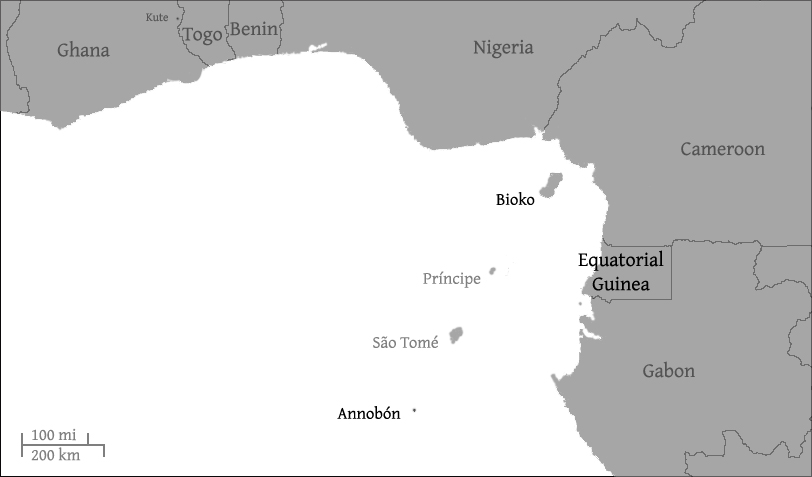
\includegraphics[width=.95\textwidth]{figures/yakpomod-img1.png}
	\label{map:1:1.1}
\end{figure}

\begin{figure}
	\caption*{Map 2 Towns with Pichi-speaking communities in Bioko (in bold)}
	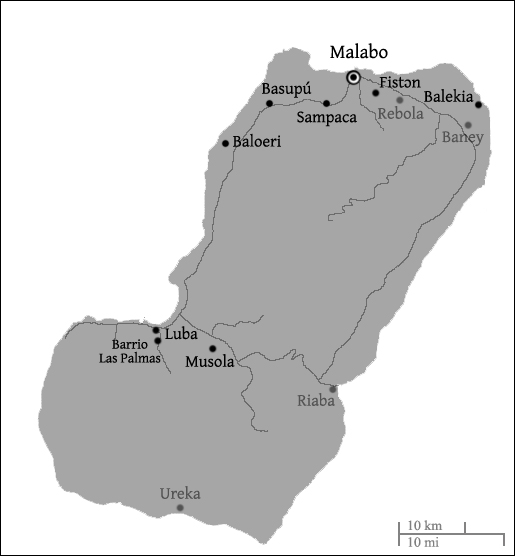
\includegraphics[width=.5\textwidth]{figures/yakpomod-img2.png}
	\label{map:1:1.2}
\end{figure}

The lingering colonialist perspective on Pichi and its sister languages in West Africa and across the Atlantic stands in stark contrast to the fact that these languages epitomise the achievements of African and African-descended peoples who, in resisting and adapting to the ignominious system of European slavery and colonialism, carved out in Africa and the Americas one of the largest, and today most vibrant cultural and linguistic zones of the world.

\section{Contact with Spanish}\label{sec:1.2}

\ili{Spanish} has left a deep imprint on the lexicon and grammar of Pichi. Codemixing is an integral part of the linguistic system of Pichi (\citealt{Yakpo2009complexity}, \citealt{Yakpo2018}). The pervasive influence of \ili{Spanish} on Pichi is for one part the consequence of language policy. Since colonial rule and the independence of Equatorial Guinea in 1968, Spanish has remained the sole medium of instruction at all levels of the educational system (\citealt[35–36]{Lipski1992}). There is a widespread competence in different registers of \ili{Spanish} by Pichi speakers in Malabo and Equatorial Guinea as a whole \citep{Lipski1985,García2016}. In Malabo, the acquisition of Spanish begins in early childhood, even for many working-class Equatoguineans with little or no school education. 

Another factor favouring codemixing is the positive attitude towards multilingualism in a highly polyglot society, against the background of a tenacious vitality of Pichi as a symbol of social identity. Presumably, Pichi-Spanish codemixing has for a long time served as a badge of identity for the population of Bioko in the course of a long history of immigration by speakers of other varieties of West African English-lexicon Creoles. Today, the language also plays an important role for the self-identification of those who grew up on the island in the face of an accelerated pace of internal migration by Equatoguineans from the mainland. \textit{Bɔ́n} \textit{na} \textit{yá,} \textit{gró} \textit{na} \textit{yá} ‘born here, grown up here’ is the mark which distinguishes Pichi-speaking islanders, irrespective of their ethnic background, from the late arrivals of mainland origin who speak little or no Pichi. 

Equally, the burgeoning oil economy of Equatorial Guinea has led to increased urbanisation, extending multi-ethnic social networks and the spread of Pichi as a native language. In such a socio-economic environment and amidst a high general competence in the official language Spanish, codemixing between Pichi and Spanish, rather than being exceptional, is consciously and confidently articulated in daily life (cf. chapter 11 for a detailed description of codemixing). Pichi is also in contact with other African languages spoken in the region, amongst them \ili{Fang} and \ili{Bube}, as well as \ili{Nigerian} and Cameroonian Pidgin (\citealt{Yakpo2013} discusses influences on Pichi from these languages).

\section{Variation}\label{sec:1.3}

The variation recorded in Pichi appears to be determined by a mixture of the factors age, language background, and social class. Phonological variation is particularly conspicuous. Some of the variation in Pichi may be captured by an albeit oversimplified division of speakers into two groups. Group 1 principally consists of the Fernandinos, the old commercial and social elite of Bioko \citep{Lynn1984} that inhabits the historical centre of Malabo and has used Pichi as a home language since the 19\textsuperscript{th} century. Group 1 also comprises people of diverse ethno-linguistic backgrounds who grew up in Malabo in the ambit of Fernandino culture. The lexicon, grammar, and phonology of Group 1 reflects an earlier chronolect of Pichi, which is also closer to (early) Krio. 

Group 2 is larger and culturally more diverse by incorporating “nuevos criollos” (Morgades Besari, p.c.) who have been accultured more recently into the Pichi-speaking urban culture of Malabo. It encompasses a large number of speakers with a \ili{Bube} cultural background who have shifted to Pichi as a primary language \citep{BolekiaBoleká2007}, and it includes large numbers of speakers with varying degrees of nativisation. Group 1 is shrinking at the expense of Group 2 through rapid urbanisation, immigration, and language shift. The terms “Mesopidgin” and “Acropidgin” employed by \citet{MorgadesBesari2011} capture some of the socio-linguistic differences between Group 1 and Group 2. The distinction between Group 1 and 2 is also reflected in apparent-time differences, where older speakers (principally those who came of age in the colonial era and the first decade of independence) tend to use the Group 1 lect, and the young majority population of Malabo and Bioko tends to use the Group 2 lect. 

In this work, I privilege the description of the language of Group 2 in the wish to represent how Pichi is spoken by the young and multi-ethnic majority in the homes and streets of Malabo today. I nevertheless account for variation by employing alternate forms where they exist (e.g. \textit{nɔ́bà{\textasciitilde}nɛ́a} ‘\textsc{neg.prf}’, \textit{tínap{\textasciitilde}tánap} ‘stand (up)’), and some of them may reflect differences between Groups 1 and 2. In the following, I present a few generalisations of the variation present in my corpus. 

For Group 2 speakers, there is no phonemic contrast between the alveolar fricative [s] and the postalveolar fricative [ʃ] (\hyperref[ex:0.1]{1}--\hyperref[ex:0.1.1]{2}), and this is systematically applied to all words where Group 1 speakers use [ʃ] (\hyperref[ex:0.2]{3}). Group 2 speakers also insert a palatal glide [j] between [s] and a following mid vowel where Group 1 uses [ʃ] alone (\hyperref[ex:0.3]{4}--\hyperref[ex:0.4]{5}):



% beginning of manual numbering of examples till (11)

% inserted ex:0.1.1 so manual numbering doesn't match with label numbering

\bigskip
\noindent\begin{tabularx}{\textwidth}{l ll lX}
% \lsptoprule
 &  & Group 1 &  Group 2 & \\
% \midrule
(1) \label{ex:0.1}
         & \itshape só & [só] & [só]  & ‘sew, like that’\\
(2) \label{ex:0.1.1}
         & \itshape só & [ʃó] & [só]  & ‘show’\\
(3) \label{ex:0.2}
         & \itshape fínis & [fínìʃ] & [fínìs] & ‘finish’\\
(4) \label{ex:0.3}
         & \itshape sɔ́p & [ʃɔ́p] & [sjɔ́p] & ‘shop’\\
(5) \label{ex:0.4}
         & \itshape nésɔn & [néʃɔ̀n] & [nésjɔ̀n] & ‘nation’\\
% \lspbottomrule
\end{tabularx}

\bigskip
Group 2 speakers tend to neutralise the phonemic distinction between close-mid and open-mid vowels (\hyperref[ex:0.5]{6}–\hyperref[ex:0.6]{7}):

\bigskip
\noindent\begin{tabularx}{\textwidth}{l ll lX}
 &  & Group 1 & Group 2 & \\
% \lsptoprule
(6) \label{ex:0.5}
         & \itshape fɔ & [fɔ̀] & [fò {\textasciitilde} fɔ̀] & ‘\textsc{prep}’\\
& \itshape mɔ́ & [mɔ́] & [mó {\textasciitilde} mɔ́] & ‘more’\\
(7) \label{ex:0.6}
         & \itshape mék & [mék] & [mék {\textasciitilde} mɛ́k] & ‘make, \textsc{sbjv}’\\
& \itshape lɛk & [lɛ̀k] & [lèk {\textasciitilde} lɛ̀k] & ‘like (preposition)’\\
% \lspbottomrule
\end{tabularx}

\bigskip
Group 2 speakers also tend to nasalise [i]-final words with an H.L tonal configuration (\hyperref[ex:0.7]{8}) and to prenasalise [j]-initial words as in (\hyperref[ex:0.8]{9}). This may lead to the formation of homophones like (\hyperref[ex:0.9]{10}) and (\hyperref[ex:0.10]{11}) for Group 2 speakers:

\bigskip
\noindent\begin{tabularx}{\textwidth}{l ll lX}
 &  & Group 1 & Group 2 & \\
% \lsptoprule
(8) \label{ex:0.7}
         & \itshape lɔ́ki & [lɔ́kì] & [lɔ́kìn] & ‘be lucky’\\
& \itshape tɔ́sti & [tɔ́stì] & [tɔ́stìn] & ‘be thirsty’\\
(9) \label{ex:0.8}
         & \itshape yandá & [jàndá] & [njàndá] & ‘yonder’\\
(10) \label{ex:0.9}
         & \itshape yús & [jús] & [njús] & ‘use’\\
(11) \label{ex:0.10}
         & \itshape nyús & [njús] & [njús] & ‘news’\\
% \lspbottomrule
\end{tabularx}



% end of manual numbering of examples
\addtocounter{equation}{11}

\bigskip
There is also some variation in the use and acceptance of certain grammatical structures. For example, Group 2 speakers seem to prefer the negative perfect marker \textit{nɛ́a} over \textit{nɔ́ba}. Equally, a serial verb construction\is{serial verb constructions} (SVC) featuring the verb \textit{sté} ‘be long time’ is not readily accepted as grammatical by many Group 1 speakers (cf. \sectref{sec:11.2.5}) and may therefore be a more recent development. Conversely, other types of SVCs are more common with Group 1 than with Group 2. Amongst them are SVCs involving the verb \textit{ték} ‘take’ (cf. \sectref{sec:11.2.3}) and motion-direction SVCs involving the verbs \textit{gó} ‘go’ and \textit{kán} ‘come’ (cf. \sectref{sec:11.2.1}). \textit{Ték}-serialisation is very common in modern \ili{Krio} and all other African English-lexifier creoles. Group 2 speakers instead tend to employ a combination of a verb and a prepositional phrase in these contexts. A final area characterised by variation is the extent of Pichi-Spanish language contact. For example, the names of weekdays and numerals are almost exclusively expressed in Spanish by Group 2 speakers. Group 1 speakers have access to both English- and Spanish-derived lexicon. They may employ \textit{lunes} ‘Monday’ in a codemixed sentence, but are equally likely to use \textit{mɔ́nde} ‘Monday’. Further, English-derived numbers above five are rarely used by Group 2 speakers (cf. \sectref{sec:13.3.1}). In contrast, Group 1 speakers master a wider range of the Pichi numeral system. However, even with this group, Pichi numbers above ten are seldom heard.

\section{Affiliation}\label{sec:1.4}
\largerpage
Pichi belongs to the grouping of languages referred to in the literature by various appelations, among them “English-based Afro-American” \citep{Alleyne1980}, “Atlantic Anglophone Creoles” \citep{Hancock1986,Hancock1987} “Atlantic English-based Creoles” (e.g. \citealt{MuyskenSmith1990}), “Atlantic English Creoles” (e.g. \citealt{Baker1999}). In this work and others, I employ the term “Afro-Caribbean English-lexifier Creoles” (abbreviated AECs) \citep{Faraclas2004} as a label that includes information about the speaker population (\mbox{“Afro-”}, i.e. people of African ancestry) and the two world regions where the languages are mainly spoken (“Afro-Caribbean”, i.e. Africa and the Caribbean). The use of “lexifier” underscores the dynamic character of the \ili{English} input to the lexicon, which varies in size and nature between the different languages. 


All Afro-Caribbean English-lexifier Creoles are transmitted and learned in various ways within the family and serve as means of communication and identification to linguistic communities. I therefore dispense with the term “pidgin” with its socio-structural connations and use “creole” alone. When referring to the linguistic grouping, “Creole” is written with an initial capital letter. The generic term is written “creole” in lower case. 

With well over 100 million speakers, the Afro-Caribbean English-lexifier Creoles and Pidgin-Creoles (henceforth AECs) spoken in Africa and the Americas together constitute one of the largest lectal continua of the Western hemisphere in speaker numbers and geographical extent \citep[22–23]{Yakpo2016estatuto}. Besides Pichi, the African sub-grouping of the AECs contains \ili{Krio} (Sierra Leone), \ili{Aku} (Gambia), Ghanaian Pidgin English, Nigerian Pidgin, and Cameroonian Pidgin \citep{HuberGörlach1996,Huber1999,BakerHuber2001}. There are also historical connections and cross-influences with varieties of Liberian English \citep{Singler1997}. Even if many details are still unclear, the evidence that there is a degree of common ancestry between the African and Caribbean AECs is compelling (e.g. \citealt{Hancock1986,Hancock1987,Smith1987,Smith2015}). There are also indications of a historical relation of the AECs with African American English(es) \citep{Dillard1973,Rickford1999,Winford2017}.

Within the African AECs, Pichi is most directly related to the \ili{Krio} language of Sierra Leone. A comparison of the two languages yields systematic lexical and structural correspondences. But it also reveals some differences. To begin with, both languages share a large percentage of non-basic vocabulary\is{basic vocabulary}, as shown in (\ref{ex:1:7}a), with the same tonal configurations. However, the Yoruba (b), Mende (c), and Temne (d) component of the Pichi lexicon appears to be much smaller than that of Krio and is limited to a few words in the corpus (data from \citealt{FyleJones1980}):

\eabox{\label{ex:1:7}
\begin{tabularx}{\textwidth}{rllX}
   & Pichi & Krio & Gloss\\
a. & \itshape a & \itshape a & ‘I’\\
& \itshape pɔ́sin & \itshape pɔ́sin & ‘person’\\
& \itshape (s)tík & \itshape (s)tík & ‘tree’\\
& \itshape yáy & \itshape yáy & ‘eye’\\
& \itshape yés & \itshape yés & ‘ear’\\
& \itshape bɔbí & \itshape bɔbí & ‘breast’\\
& \itshape bɛlɛ́ & \itshape bɛlɛ́ & ‘belly, foetus’\\
& \itshape watá, wɔtá & \itshape watá, wɔtá & ‘water’\\
& \itshape dɔtí & \itshape dɔtí & ‘be dirty’\\
& \itshape fɔdɔ́n & \itshape fɔdɔ́m & ‘fall’\\
& \itshape chɔ́p & \itshape chɔ́p, ít & ‘eat’\\
& \itshape hós & \itshape hós & ‘house’\\
& \itshape tití & \itshape tití & ‘girl’\\
& \itshape mákit & \itshape mákit, mákɛt & ‘market’\\
& \itshape wɔwɔ́ & \itshape wɔwɔ́ & ‘be messed up, ugly’\\
& \itshape bɔkú & \itshape bɔkú & ‘be much’\\
& \itshape yangá & \itshape nyangá & ‘be ostentatious’\\
& \itshape dúya & \itshape dúya & ‘please’\\
b. & \itshape ógi & \itshape ógi & ‘corn porridge’\\
& \itshape kúsɛ́ & \itshape kúshɛ́ & ‘expression of empathy’\\
& \itshape {}--- & \itshape órewá & ‘goodbye greeting’\\
c. & \itshape nyɔ́ní & \itshape nyɔ́ní & ‘red ant’\\
& \itshape blɔkɔ́s & \itshape blɔkɔ́s & ‘scrotum, penis’\\
& \itshape kandá & \itshape kandá & ‘skin, bark’\\
d. & \itshape yabaś & \itshape yabás & ‘onion’\\
& \itshape {}--- & \itshape kunkubé & ‘kind of boat’\\
\end{tabularx}
}
The two languages also share a number of lexical items common to numerous African and American English-lexicon Creoles. These were first compiled by (\citealt{Smith1987,Smith2001,Smith2015}) and termed “Ingredient X, Y, and Z”. In \REF{ex:1:8}, I list all the relevant words contained in the Pichi corpus. They comprise “Ingredient X” words of African origin (a), “Ingredient Y” words of Portuguese origin (b), “Ingredient Z” words of English origin (c), as well as a few function words of diverse origin (d):

\eabox{\label{ex:1:8}
\begin{tabularx}{.9\textwidth}{rll}
         & Ingredient X, Y, Z & Gloss\\
a. & \itshape sósó & ‘only’\\
& \itshape pɔtɔpɔ́tɔ́ & ‘mud(dy) substance’\\
& \itshape akará & ‘bean cake’\\
& \itshape fufú & ‘fufu’\\
b. & \itshape sabí & ‘know’\\
& \itshape pikín & ‘child’\\
c. & \itshape kéch & ‘catch’\\
& \itshape yɛ́r(i) & ‘hear’\\
& \itshape ɛf(ɛ) & ‘if’\\
& \itshape bwɛ́l & ‘boil’\\
& \itshape (s)pwɛ́l & ‘spoil, spend’\\
d. & \itshape na & ‘\textsc{foc}’\\
& \itshape una, unu & ‘\textsc{2pl}’\\
& \itshape mék & ‘imperative\is{imperatives}, \textsc{sbjv}’\\
& \itshape de & ‘\textsc{ipfv}’\\
& \itshape dé & ‘there’\\
& \itshape dé & \textsc{‘be.loc’}\\
\end{tabularx}
}
Some of the differences in vocabulary between the two languages owe to the same phonological characteristics that differentiate the members of Group 1 (Pichi) and Group 2 (\ili{Krio}) in the preceding section. Hence, most speakers of Pichi make no phonemic distinction between alveolar and postalveolar fricatives (\ref{ex:1:9}a); the phonemic distinction between close-mid and open-mid vowels is neutralised by most speakers (b). 

In addition, the distinction between velar and labial nasal consonants tends to collapse in word-final position (c); phonological processes create preferred CV sequences (d), voiced obstruents are normally devoiced in word-final position (e), while other words have different coda consonants (f). In general terms, present-day Pichi as spoken by the majority of its speakers exhibits a tendency towards the reduction of phonemic contrasts when compared to Krio.

\eabox{\label{ex:1:9}
\begin{tabularx}{\textwidth}{r ll ll ll}
 & \multicolumn{2}{l}{Pichi} & \multicolumn{2}{l}{Krio} & Gloss\\
a. & \itshape sút & [sút] & \itshape shút & [ʃút] & ‘shoot’\\
b. & \itshape fɔ & [fɔ̀{\textasciitilde}fò] & \itshape fɔ & [fɔ̀] & ‘\textsc{prep}’\\
c. & \itshape frɔn & [frɔ̀n {\textasciitilde} frɔ̀m] & \itshape frɔm & [frɔ̀m] & ‘from’\\
d. & \itshape smɔ́l & [sìmɔ́ {\textasciitilde} sùmɔ́] & \itshape smɔ́l & [smɔ́l] & ‘be small’\\
e. & \itshape bíg & [bík] & \itshape bíg & [bíg] & ‘be big’\\
f. & \itshape (s)trɔ́n & [(s)trɔ́n] & \itshape (s)trɔ́ng & [(s)trɔ́ŋ] & ‘be strong’\\
\end{tabularx}
}
Other differences in vocabulary, phonology, and grammar stem from the divergent socio-political development that Equatorial Guinea and Sierra Leone have gone through in the last hundred years. In Sierra Leone, British colonisation and the retention of political, economic, and linguistic ties with Britain after independence have reinforced the relationship between \ili{Krio} and \ili{English}. In Equatorial Guinea, the direct link with \ili{English} was severed in 1858 when Spanish assumed the role of the dominant language. Equally, the influence of \ili{Krio} on Pichi had petered out by the first decades of the 20\textsuperscript{th} century as Spanish colonialism gradually put a stranglehold on relations between Fernando Po and Sierra Leone. 

The role of the respective superstrates \ili{English} (for \ili{Krio}) and \ili{Spanish} (for Pichi) can be read from the impact of these two languages on institutional and administrative terminology (\ref{ex:1:10}a), the numeral system above ten (b), and other lexical items (c). The use of a larger number of English-derived lexical items in \ili{Krio} corresponds with a stronger presence of Spanish-derived lexicon in Pichi:

\eabox{\label{ex:1:10}
\begin{tabularx}{\textwidth}{rlll}
         & Pichi & Krio & Gloss\\
a. & \itshape profe(sor), tícha & \itshape tícha & ‘teacher’\\
& \itshape Camerún & \itshape Cameroon & ‘Cameroon’\\
& \itshape aeropuerto & \itshape ɛ́pɔt & ‘airport’\\
b. & \itshape diez & \itshape tɛ́n & ‘ten’\\
& \itshape doce & \itshape twɛ́lf & ‘twelve’\\
& \itshape las dos & \itshape tú oklɔ́k & ‘two o’clock’\\
c. & \itshape bikɔs, porque & \itshape bikɔs & ‘because’\\
& \itshape sube, gó ɔ́p & \itshape gó ɔ́p & ‘go up’\\
& \itshape sigue & \itshape kɔntínyu & ‘continue’\\
\end{tabularx}
}
There is a high degree of correspondence between the forms of Pichi and \ili{Krio} function words and the categories they express. For example, the forms and functions of the TMA\is{tense}\is{modality}\is{aspect} markers in \REF{ex:1:11} are largely coterminous: 

\eabox{\label{ex:1:11}
\begin{tabularx}{\textwidth}{llll}
Pichi & \ili{Krio} & Gloss\\
\itshape de & \itshape de & ‘\textsc{ipfv’}\\
\itshape go & \itshape go & ‘\textsc{pot}’\\
\itshape bin & \itshape bin & ‘\textsc{pst}’\\
\itshape dɔ́n & \itshape dɔ́n & ‘\textsc{prf}’\\
\itshape fɔ & \itshape fɔ & ‘\textsc{prep}’\\
\itshape kin & \itshape kin & ‘\textsc{hab}, \textsc{abl’}\\
\end{tabularx}
}
However, the distribution of the markers in \REF{ex:1:11} is not always identical in the two languages. For example, the \ili{Krio} data reveals more combinatorial possibilities of the habitual\is{habitual aspect} marker \textit{kin} ‘\textsc{hab}’ with other TMA markers (cf. \citealt{Dandeson2001}), while the Pichi imperfective marker \is{imperfective aspect} \textit{de} ‘\textsc{ipfv}’ seems to have a broader range of functions than the \ili{Krio} cognate form. Moreover, \ili{Krio} has at least two auxiliary constructions which are not attested in my data. The verb \textit{blánt} is only employed as a lexical verb with the meaning ‘reside’ in Pichi. In \ili{Krio}, the element \textit{blant} is a preverbal TMA element that expresses habitual aspect. Further evidence for grammaticalisation is that \textit{blant} is L-toned in this function. Consider the following example (Krio sentences are marked \textsc{Krio}):

\newpage 
\ea%12
    \label{ex:1:12}
\textsc{Krio}\il{Krio}\\
    \gll   Olú    \textbf{blant}  \textbf{gó}  London  fɔ  Krísmɛs.\\
\textsc{name}  \textsc{hab}    go  \textsc{place}  \textsc{prep}  Christmas\\

\glt ‘Olu always goes to London for Christmas.’  \citep[181]{YillahCorcoran2007}
\z

Further, \ili{Krio} employs the locative-existential copula \textit{dé} \textsc{‘be.loc’} together with the preposition \textit{pan} ‘on’ in an, albeit lectally restricted, auxiliary construction to express \isi{progressive aspect} \REF{ex:1:13}. The construction is rejected by Pichi speakers \REF{ex:1:14}:


\ea%13
    \label{ex:1:13}
\textsc{Krio}\il{Krio}\\
    \gll   \textit{Olú}   \textbf{dé}   \textbf{pan}    kám.\\
\textsc{name}  \textsc{be.loc}  on    come\\

\glt ‘Olu is coming (right now).’ \citep[179]{YillahCorcoran2007}
\z


\ea[*]{%14
    \label{ex:1:14}
    \gll   A    \textbf{dé}    \textbf{pan}   chɔ́p.\\
 \textsc{1sg.sbj}  \textsc{be.loc}  on    eat\\
\glt Intended: ‘I’m eating.’ [ye07je 025]
}\z

Conversely, there is no data to suggest the existence in \ili{Krio} of the Pichi egressive aspect construction involving the auxiliary verb \textit{kɔmɔ́t} ‘go/come out’ \REF{ex:1:15} or, obviously, the continuative aspect construction featuring the Spanish-derived verb \textit{sigue} ‘continue’ \REF{ex:1:16}. Equally, an adverbial SVC involving the V1 \textit{sté} ‘stay, be a long time’ appears to be unique to Pichi \REF{ex:1:17}: 


\ea%15
    \label{ex:1:15}
    \gll   Wì  \textbf{kɔmɔ́t}    \textbf{chɔ́p}  náw    só.\\
 \textsc{1pl}  come.out  eat    now    like that.\\
\glt ‘We just ate right now.’ [ge07fn 208]
\z


\ea%16
    \label{ex:1:16}
    \gll   A    \textbf{sigue}    \textbf{plé}    bɔ́l  sóté    ívin    tɛ́n.\\
\textsc{1sg.sbj}  continue    play    ball  until  evening  time\\

\glt ‘I continued playing ball until the evening.’ [be07fn 189]
\z


\ea%17
    \label{ex:1:17}
    \gll   A    \textbf{sté}  \textbf{chɔ́p}.\\
\textsc{1sg.sbj}  stay    eat\\

\glt ‘It’s been a long time since I ate.’ [au07ec 078]
\z

The literature on \ili{Krio} also indicates a wider range and a more pervasive use of SVCs than attested for Pichi. For instance, \ili{Krio} has a resultative SVC \is{resultative SVC}featuring dynamic verbs in the V2 position \REF{ex:1:18} and a \textsc{give}{}-type SVC in order to mark a recpient or beneficiary \REF{ex:1:19}. Both types of construction are not attested in Pichi:


\ea%18
    \label{ex:1:18}
\textsc{Krio}\il{Krio}\\
    \gll   Di  húman  \textbf{kúk}    rɛ́s    \textbf{sɛ́l}.                  \\
    \textsc{def}  woman  cook  rice    sell\\
\glt ‘The woman cooked rice and sold it.’ \citep[72]{Finney2004}
\z

\ea%19
    \label{ex:1:19}
\textsc{Krio}\il{Krio}\\
    \gll   I    \textbf{báy}    klós    \textbf{gí}    in    pikín.\\
\textsc{3sg.sbj}  buy    clothing  give    \textsc{3sg.poss}  child\\

\glt ‘He bought some clothes for his child.’ \citep[72]{Finney2004}
\z

In contrast, resultative state of affairs similar to \REF{ex:1:18} above may only feature stative property items as secondary verbs. Such constructions in Pichi are best seen to involve secondary predication \REF{ex:1:20}:


\ea%20
    \label{ex:1:20}
    \gll   Dɛn    dɔ́n    \textbf{bíl}   di  hós    \textbf{strɔ́n}.\\
\textsc{3pl}    \textsc{pfv}    build  \textsc{def}  road    be.strong\\

\glt ‘The house is solidly built.’ [ra07ve 069]
\z

At the same time, Pichi only employs a less integrated type of multiverb construction, namely clause chaining, in order to express a sentence like \REF{ex:1:19}, involving a dynamic V2. Note that unlike the \ili{Krio} sentences above, the Pichi example in \REF{ex:1:21} exhibits resumptive\is{resumptive pronouns} subject marking, i.e. the subject is repeated with the second verb in the series: 


\ea%21
    \label{ex:1:21}
    \gll   \textbf{Yu}  \textbf{ték}    di  mɔní  \textbf{yu}  \textbf{gí}  mí.\\
\textsc{2sg}  take    \textsc{def}  money  \textsc{2sg}  give  \textsc{1sg.indp}\\

\glt ‘You took the money (and) gave it to me.’ [ro05de 033]
\z

Numerous questions, however, remain open with regard to the extent of differences between the two languages. A considerable obstacle to comparative research is the lack of fresh data on Krio since the 1980s.

\section{Previous research on Pichi}\label{sec:1.5}

\citealt{Yakpo2009a} (in English) and \citeyear{Yakpo2010} (in Spanish) are the first in-depth descriptions of the phonology and grammar of Pichi. \citet{Zarco1938} is a language guide with a vocabulary list and a short grammar section. Trinidad Morgades Besari, former Vice-Chancellor of the National University of Equatorial Guinea and a well-known philologist of the country, has written about the use of \ili{Spanish} and Pichi in Equatorial Guinea \citep{MorgadesBesari2005,MorgadesBesari2011}. Morgades Besari’s unpublished work encompasses wordlists, a collection of stories and proverbs and proposals for an orthography of Pichi (see \citealt{Yakpo2011} for a discussion of the orthography). CEIBA Ediciones (Barcelona) has published a series of works dealing with the precolonial and colonial history and the political economy of Fernando Po, as well as the pivotal role of the Fernandinos in the making of present-day Bioko (e.g. \citealt{MartindelMolino1993}; \citealt{Cantús2006}).

\section{Standardisation and orthography}\label{sec:1.6}

No commonly accepted standard orthography is in use for Pichi. The transcription used in this work follows the Krio orthography employed in the seminal Krio-English Dictionary \citep{FyleJones1980} and subsequent revisions \citep{Coomber1992}, which, in turn, relies on the IPA-based Africa Alphabet \citep{InternationalAfricanInstitute1930} and the African Reference Alphabet \citep{UNESCO1981}. In the Krio\slash Pichi orthography, the grapheme <ɛ> renders the open-mid front vowel [ɛ], and <ɔ> renders the open-mid back vowel [ɔ]. Other vowel graphemes approximately also represent the corresponding IPA sounds. Pichi consonant phonemes and graphemes are presented in \tabref{tab:key:2.1}. In codemixed sentences, Spanish material is rendered using the standard Spanish orthography. 


Tone is marked on all Pichi words throughout this book. H-toned syllables bear an acute accent, e.g. \textit{wét} [wét] ‘wait’, and L-toned syllables remain unmarked, e.g. \textit{wet} [wèt] ‘with’. Tonal notation applies to the morpheme (i.e. the root), not the phonological word. In multimorphemic words, each morpheme therefore receives separate tone marks, e.g. \textit{ús=tɛ́n} \{\textit{\'us} ‘\textsc{q}’, \textit{tɛ́n} ‘time’\} ‘when’, \textit{fáyn-wán} \{\textit{fáyn} ‘nice’, \textit{-wán} ‘\textsc{adv}’\} ‘nicely’. Acute accents over Spanish words are orthographic, and hence not tone marks.


\section{Methods and data}\label{sec:1.7}

This grammatical description of Pichi is based on the analysis of a corpus of 46,060 words of dialogues, narratives, procedural texts, and elicitations. The data was collected during three stays of four weeks each in Malabo between 2003 and 2007 as part of the research for my PhD thesis \citep{Yakpo2009a}. Recordings were conducted in the quarters of Ela Nguema, Nyumbili, and the historical centre of Malabo. Recordings were done with a digital mini disc recorder and transcribed and analysed using the SIL Toolbox 1.5 programme. The analysis of tone was done from connected speech and words spoken in isolation using the Praat 5.0 software \citep{boersma2008}. Much of my approach is guided by linguistic typology and the descriptive apparatus developed in research on African languages. I try to describe as much variation as feasible. I largely avoid comparative or etymological observations with respect to English and African languages and try to look at Pichi “from the inside”. This grammar has also been published in Spanish \citep{Yakpo2010} in an abridged version for use in Equatorial Guinea by researchers and university students, teachers, and educationists. 


In Equatorial Guinea, I worked with altogether seventeen language consultants. All speakers have been using Pichi continuously since childhood onwards. Without exception, they are inhabitants of Malabo since birth or infancy. Most of them use Pichi more often than any other language, and most speakers view Pichi as the language they know best. Additionally, all speakers also know at least one of the following other languages in varying degrees of proficiency: \ili{Fang}, \ili{Bube}, \ili{Fa d’Ambô}, \ili{Kombe}, \ili{Lungwa Santome}, Nigerian Pidgin, \ili{Twi}, \ili{Spanish}, \ili{French}, \ili{English}, and \ili{German}. There is a bias in the data towards speakers with a Bube ethno-linguistic background, reflective of the circumstance that the majority of people who use Pichi as their primary language are from a Bube background. The numerical dominance by these “nuevos criollos” over the “old” Creole community of Fernandino descent (Morgades Besari, p.c.) represents a significant shift in the social dynamics of the language which is reflected in my choice of speakers. 



A few words are in order on aspects of my linguistic background and communicative approach during the research leading to this book. During my first stay in Malabo, I used Ghanaian Pidgin English and Spanish as working languages. During subsequent visits, when I felt confident enough to use Pichi without impeding fluid communication, I conducted my research exclusively in Pichi. My acquisition of Pichi and integration into social networks in Malabo was greatly facilitated by fluency in Ghanaian Pidgin English, competence in, and exposure to other Afro-Caribbean English-lexifier Creoles and West African languages, and a cultural and communicative \textit{savoir} \textit{faire} acquired during a childhood spent in Ghana. Fluency in French and Portuguese were also important resources in navigating the plurilingual landscape of Malabo and Bioko at various junctures during my research.


\tabref{tab:1:1.1} lists relevant information on language consultants. Speakers are sorted alphabetically along the “code” column. The symbol “N.N.” in the last row of the “speaker” column stands for incidental data collected from strangers in the streets, markets, and other public places in Malabo. Not included in the list is my own speaker code (ko). My participation in recorded conversations was kept to a minimum, but due to the nature of the method, it was more extensive during elicitations. Utterances of mine are, however, nowhere included in the analyses and interpretation of data. The symbols for gender are (F)emale and (M)ale. Age is provided in brackets of 10+, 20+, 30+, etc. The column “languages” specifies self-identified language knowledge. The symbol~(h) in the “languages” column indicates home languages used for interaction within the (extended) family. Languages are listed in alphabetical order but home languages come first. Basic information on social class can be deduced from the “activity” column. The column “residence” indicates the neighbourhood of Malabo in which the respective speakers are domiciled. Detailed information on the corpus is provided in \tabref{tab:1:1.2} further below.

%%please move \begin{table} just above \begin{tabular
%\begin{table}

\begin{longtable}{>{\footnotesize}l@{~}>{\footnotesize}l@{~} >{\footnotesize}l@{~}>{\footnotesize}l >{\footnotesize\raggedright}p{3cm} >{\footnotesize\raggedright}p{2cm} >{\footnotesize}l}
\caption{Language consultants}\label{tab:1:1.1}
\\
\lsptoprule

Code & Speaker & F/M & Age & Languages & Activity & Residence\\
\midrule\endhead
ab & Abuela & \textsc{F} & 80+ & Bube~(h), Pichi~(h), 

Spanish~(h) & Child rearing, farming & Town\\
au & Agustín & M & 30+ & Fang~(h), Spanish~(h), Pichi, French & Senior civil service & Ela Nguema\\
be & Beatriz & \textsc{F} & 20+ & Bube~(h), Pichi~(h), Spanish & Child rearing & Ela Nguema\\
bo & Aboki & \textsc{F} & 40+ & Pichi~(h), Spanish~(h), Bube & Trade & Town\\
ch & Charlie & M & 10+ & Pichi~(h), Spanish & School goer & Ela Nguema\\
dj & Djunais & M & 20+ & Pichi~(h), Spanish~(h), Bube & Cook & Ela Nguema\\
eb & Ebongolo & M & 20+ & Kombe ~(h), Pichi, Spanish &  & Ela Nguema\\
ed & Eduardo & M & 30+ & Fa d’Ambô~(h), Lungwa Santome~(h), Fang, English, Pichi, Spanish & Civil servant & Ela Nguema\\
f1 & Fita 1 & M & 20+ & Unknown & Mechanic & Nyumbili\\
f2 & Fita 2 & M & 20+ & Unknown & Mechanic & Nyumbili\\
fr & Francisca & \textsc{F} & 30+ & Pichi~(h), Spanish~(h), English, French & Civil servant & Ela Nguema\\
ge & Lage & \textsc{F} & 30+ & Pichi~(h), Spanish~(h), English & Restaurant owner & Ela Nguema\\
he & Hermina & \textsc{F} & 30+ & Kombe ~(h), Fang, Pichi, Spanish & Child rearing & Ela Nguema\\
hi & Hilda & \textsc{F} & 50+ & Pichi~(h), Spanish~(h), Bube, English & Trade & Town\\
ku & Tía Kuki & \textsc{F} & 50+ & Kombe ~(h), Fang, Pichi, Spanish & Trade & Ela Nguema\\
kw & Kwame & M & 40+ & Twi~(h), English, Pichi, Spanish & Security guard & Kolwatá\\
li & Lindo & M & 30+ & Kombe ~(h), Pichi~(h), Spanish & Worker & Ela Nguema\\
lo & Lourdes & \textsc{F} & 30+ & Pichi~(h), Spanish~(h), English & Manager & Town\\
ma & María & \textsc{F} & 30+ & Bube~(h), Pichi~(h), Spanish & Domestic worker & Nyumbili\\
mi & Miguel & M & 10+ & Pichi~(h), Spanish~(h), Bube & School goer & Town\\
ne & Nenuko & M & 30+ & Pichi~(h), Spanish~(h), Bube & Mechanic & Ela Nguema\\
pa & Pancho & M & 20+ & Pichi~(h), Spanish~(h), Bube & Hustler & Ela Nguema\\
ra & Maura & \textsc{F} & 20+ & Pichi~(h), Spanish~(h), Bube & Secretary & Los Angeles\\
ro & Mami Rose & \textsc{F} & 50+ & Bube~(h), Pichi~(h), Spanish & Domestic worker & Ela Nguema\\
sa & Don Samuel & M & 70+ & Kombe ~(h), Fang, Pichi, Spanish & Entre-preneur & Town\\
to & Tía Tokó & \textsc{F} & 50+ & Bube~(h), Pichi~(h), Spanish~(h), Nigerian Pidgin, English & Accountant & Town\\
tr & Doña Trinidad & \textsc{F} & 70+ & Pichi~(h), Spanish~(h), English, French & Academic & Town\\
ur & Ursus & M & 30+ & Pichi~(h), Bube, Spanish & Worker & Ela Nguema\\
ye & Boyé & M & 20+ & Pichi~(h), Spanish~(h), Bube & Worker & Ela Nguema\\
nn & N.N & M/\textsc{F} & Div. & Diverse & Diverse & Diverse\\
\lspbottomrule
\end{longtable}
%\end{table}

\tabref{tab:1:1.2} provides information on the corpus. The list is sorted alphabetically according to the “text code” column, which lists the name of the text (e.g. 03ab). Text names were given according to mnemonic principles. An “e” at the end of text code indicates that the text consists of elicited data (e.g. 05ae). The “type” column indicates the text genre, “contents” provides a short description of the text. The column entitled “word count” provides an indication of the relative length of texts. An asterisk (*) after the “text code” indicates that the corresponding text is contained (in part or in full length) in the text section of this book.

%%please move \begin{table} just above \begin{tabular
%\begin{table}

\begin{longtable}{l >{\raggedright}p{2.1cm} >{\raggedright}p{4.5cm} lr}
\caption{Corpus}\label{tab:1:1.2}\\
\lsptoprule

Text & Type & Contents & Speakers & Word\\
code & & & & count\\
\midrule
\endhead
03ab* & Narrative & Sickness & ab, fr & 1911\\
03ay & Narrative & Youth memories & ab & 2384\\
03cb & Conversation & Female-male relations & hi, bo & 2872\\
03cd* & Conversation & House-building; joking; home affairs & dj, fr, ko, ye & 1827\\
03do* & Procedure & Preparation of a dish & dj & 778\\
03ft & Narrative & Family history & fr & 2771\\
03wt* & Narrative; conversation & Supernatural encounter & dj, fr, ru & 813\\
03fp & Procedure & Car maintenance & f1, f2, kw & 274\\
03gm & Narrative & Language issues & to & 683\\
03hm & Narrative & Working in Gabon & ma & 3983\\
03ni & Conversation & Life in Nyumbili & ma, ko & 468\\
03sb & Narrative; procedure & Supernatural encounters & ed, kw & 3073\\
03sh & Narrative & Anecdotal story & ma & 291\\
03sp & Narrative & Student days in Cuba & ed, kw & 1324\\
05ae & Elicitation & Complementation; lexical aspect & dj, ye & 1930\\
05be & Elicitation & Spatial relations & dj & 1431\\
05ce & Elicitation; conversation & Basic vocabulary; metalinguistic discussion & dj, pa, ye & 2329\\
05de & Elicitation & Relativisation; adverbial relations; questions & ro & 620\\
05ee & Elicitation & Copula meanings & ro & 1101\\
05fe & Elicitation & Colours, numbers, time & ro & 256\\
05rr & Conversation; procedure & Cooking at home & ro, ye & 1278\\
05rt & Narrative & Marital affairs & ro, ye & 891\\
07ae & Elicitation & Grammatical relations & dj & 3213\\
07ce & Elicitation & Derivation & au & 739\\
07de & Elicitation & Double objects & ye & 205\\
07he & Elicitation & Questions; conversation & be, lo & 242\\
07je & Elicitation & Pragmatic routines & ye & 1072\\
07fn & Conversation & Field notes & Diverse & 1304\\
07ga* & Conversation & Anecdotal story; joking & la, ne, ye & 430\\
07me & Elicitation & Multiverb constructions & pa & 1077\\
07pe* & Elicitation (video) & Caused positions & li, dj & 783\\
07re & Elicitation (video) & Reciprocity & dj & 494\\
07se & Elicitation (video); conversation & Staged events; metalinguistic discussion & au, fr, ra & 2649\\
07ve & Elicitation & Derivation & ra & 571\\
\lspbottomrule
\end{longtable}
%\end{table}
The corpus presented in \tabref{tab:1:1.2} consists of altogether thirty-four texts of different genres totalling 46,060 words. Based on the figures of the “word count” column, narratives constitute approximately 37 per cent of the total corpus (the word count of texts with two genres has been divided by two). This genre encompasses life stories and family histories, illness and near-death accounts, supernatural encounters and other emotionally charged experiences, as well as travel and life abroad. Conversations amount to 25 per cent of the corpus. The topics range from house-building to gender relations, from jesting and joking to metalinguistic discussions during elicitation. In many of the conversations recorded, in particular those involving peer-to-peer communication, form is just as important as content. These conversations “for their own sake” are characterised by emphatic, expressive, and figurative language. 

Procedural texts form some 7 per cent of the corpus. They describe various types of routines, for example the preparation of dishes, car maintenance and repair, medical treatment and sorcery, habits and ways of doing things. Elicitation makes up about 33 per cent of the corpus. I employed oral (Spanish to Pichi and monolingual Pichi-based) elicitation to obtain data chiefly on grammatical relations, the classification of situations (i.e. dynamic vs. non-dynamic verbs vs. adjectives), complementation, relativisation, and derivation. I made use of visual, video-based elicitation to uncover the expression of spatial relations including caused positions, the expression of certain complex events (“staged events”), and reciprocity. The video clips of the Language and Cognition Group of the Max-Planck Institute for Psycholinguistics in Nijmegen provided the basis for these elicitiations. Most elicitations were conducted in groups of two or three speakers. This produced valuable data on variation and encouraged vivid metalinguistic discussions during the exercise. 

\section{Presentation of the data}\label{sec:1.8}
% \figref{fig:1:1.1} below shows how language data is presented in this work. Explanations are provided for the elements in the example:
% 
% \begin{figure}
% \caption{1 Presentation of data}
% \label{fig:1:1.1}
%  Relevant features in \textbf{bold}\\
% \begin{exe}
% \exi{\textsf{Example no.}} 
% \exi{(22)}
%  \gll A    kɛ́r=an      gó  na  comedor. \textsf{\upshape Pichi line}\\
% \textsc{1sg.sbj}  carry=\textsc{3sg.obj}    go  \textsc{loc}  dining-room \textsf{Interlinear gloss line}\\
% \glt ‘I carried him to the dining-room.’ \textsf{Free translation line}  [{ab}{03}{ab} {091}] \textsf{code}\\
% % \tikzmark{y1}{Speaker name} \hspace*{2cm} \tikzmark{y2}{year recorded}\hspace*{2cm}  \tikzmark{y3}{text name}\hspace*{2cm}  \tikzmark{y4}{sentence no. in text}
% \end{exe}
% % \connect{x1}{y1}
% % \connect{x2}{y2}
% % \connect{x3}{y3}
% % \connect{x4}{y4}
% \todo[inline]{braucht man vllt nicht. Erklärung der Codes wäre ausreichend IMHO}
% \end{figure}

In examples, the free translation is followed by a text code in squared brackets. Whenever an example features elicited data, the second letter of the text code is an “e”, e.g. [dj07ae 137] and [ra07ve 069]. Common parentheses in the free translation line contain supplementary and disambiguating translation material. Squared brackets provide contextual or other relevant meta-information. Punctuation in the Pichi examples follows intonation: A full stop indicates an utterance-final boundary tone, a comma continuative intonation. A slash denotes a speech interruption and hence an incomplete sentence. \ili{Spanish} words are rendered in the Spanish orthography. I do not provide category labels for Spanish grammatical morphemes where they occur, since this would have complicated interlinear glossing and given Spanish material undue prominence. 

A final note is in order on the notion of frequency employed throughout this work. When an exact percentage is not given, certain expressions may indicate the relative frequency or importance of a phenomenon. The expressions in the left column of \tabref{ex:1:23} correspond approximately to the percentages given in the right column \citep{MichaelisEtAl2013}.

\begin{table}
\caption{Frequency of phenomena}
\label{ex:1:23}
\begin{tabularx}{\textwidth}{lY}
\lsptoprule
Expression& Approximate percentage\\
\midrule 
Pervasive, the overwhelming majority, the vast majority & 90\%\\
The majority, very common, a high frequency & 70\%\\
About half, equally often, fairly common & 50\%\\
The minority, a low frequency & 30\%\\
Marginal, a small minority, a small number, seldom, rare & 10\%\\
\lspbottomrule
\end{tabularx}
\end{table}

  %add a percentage sign in front of the line to exclude this chapter from book
\chapter{Segmental phonology}

The phonological system of Pichi features a phoneme inventory of twenty-two consonants and seven vowels. There is a good deal of free and allophonic variation in the use of these phonemes. Phonological processes include nasalisation, the use of clitics and the appearance of a linking /r/ during cliticisation, as well as the reduction of consonant clusters by deletion and insertion. In general, however, Pichi speakers tend to fully articulate consonants and vowels. The majority of Pichi words consist of one or two syllables. There are no phonemic long vowels but words may feature clusters of up to three consonants. The segmental system of Pichi interacts in various ways with the suprasegmental system (cf. chapter 3).

\section{Consonants}\label{sec:2.1}

The maximal inventory of twenty-two consonant phonemes in Pichi is presented in IPA symbols in \tabref{tab:key:2.1}. Details on the status and distribution of these phonemes are discussed in sections \sectref{sec:2.2} and \sectref{sec:2.6.2.1}.

%%please move \begin{table} just above \begin{tabular
\begin{table}
\caption{Consonant and approximant phonemes}
\label{tab:key:2.1}
\fittable{
\small
\begin{tabular}{lllllllllllllllll}
\lsptoprule

& 
 \multicolumn{2}{p{15mm}}{Bilabial} &
 \multicolumn{2}{p{15mm}}{Labio-dental} & 
 \multicolumn{2}{p{15mm}}{(Post-)\newline alveolar} & 
 \multicolumn{2}{c}{Palatal} & 
 \multicolumn{2}{c}{Velar} & 
 \multicolumn{2}{p{10mm}}{Labio-velar} & 
 \multicolumn{2}{c}{Uvular} & 
 \multicolumn{2}{c}{Glottal}\\
\midrule 
Stop & p & b &  &  & t & d &  &  & k & g & kp & gb &  &  &  & \\
Affricate &  &  &  &  & tʃ & dʒ &  &  &  &  &  &  &  &  &  & \\
Fricative &  &  & f & v & s &  &  &  &  &  &  &  &  & ʁ &  & h\\
Nasal &  & m &  &  &  & n &  & ɲ &  & ŋ &  &  &  &  &  & \\
Liquid &  &  &  &  &  & l &  &  &  &  &  &  &  &  &  & \\
Approximant &  &  &  &  &  &  &  & j &  & w &  &  &  &  &  & \\
\lspbottomrule
\end{tabular}
}
\end{table}
The (near-)mininal pairs in \tabref{tab:key:2.2} establish the phonemic status of the segments contained in \tabref{tab:key:2.1}.

%%please move \begin{table} just above \begin{tabular
\begin{table}
\caption{Consonant phoneme minimal pairs}
\label{tab:key:2.2}

\begin{tabularx}{\textwidth}{Qlll@{\qquad\qquad} lll}
\lsptoprule
/p/  /b/ & \itshape plánt & [plánt] & ‘plant’ & \itshape blánt & [blánt] & ‘reside’\\
/t/  /d/ & \itshape tɛ́n & [tɛ́n] & ‘time’ & \itshape dɛ́n & [dɛ́n] & ‘\textsc{3pl.indp}’\\
/k/  /g/ & \itshape kɔ́n & [kɔ́n] & ‘corn’ & \itshape gɔ́n & [gɔ́n] & ‘gun’\\
/tʃ/  /dʒ/ & \itshape chɔ́ch & [tʃɔ́tʃ] & ‘church’ & \itshape jɔ́ch & [dʒɔ́tʃ] & ‘(to) judge’\\
/f/  /p/ & \itshape fát & [fát] & ‘fat’ & \itshape pát & [pát] & ‘part’\\
/v/  /b/ & \itshape greví & [grèví] & ‘gravy’ & \itshape bebí & [bèbí] & ‘baby’\\
/s/  /t/ & \itshape sɔn & [sɔ̀n] & ‘some’ & \itshape tɔ́n & [tɔ́n] & ‘town’\\
/r/  /l/ & \itshape rɔ́n & [rɔ́n] & ‘run’ & \itshape lɔ́n & [lɔ́n] & ‘be long’\\
/h/  ø & \itshape hól & [hól] & ‘hole’ & \itshape ól & [ól] & ‘be old’\\
/m/  /n/ & \itshape motó & [motó] & ‘car’ & \itshape nóto & [nótò] & ‘\textsc{neg}.\textsc{foc}’\\
/ŋ/  /n/ & \itshape tɔ́n & [tɔ́n] & ‘town’ & \itshape tɔ́ng & [tɔ́ŋ] & ‘tongue’\\
/ɲ/  /y/ & \itshape nyú & [ɲú] & ‘be new’ & \itshape yú & [jú] & ‘\textsc{2sg.indp}’\\
/j/  /w/ & \itshape yés & [jés] & ‘ear’ & \itshape wés & [wés] & ‘buttocks’\\
/kp/ /gb/ & \itshape kpu & [kpù] & ‘\textsc{ideo}’ & \itshape gbin & [gbìn] & ‘\textsc{ideo}’\\
\lspbottomrule
\end{tabularx}
\end{table}
\section{Consonant allophony and alternation}\label{sec:2.2}

/\textbf{b}/ and /\textbf{v}/:

The voiced labio-dental plosive /v/ is a phoneme in its own right in a small number of words, where it does not alternate with /b/, e.g. \textit{greví} [grèví] ‘gravy’ and \textit{gív=an} [gívàn] ‘give him/her/it’. In a second group of words, /v/ is in free variation with /b/, e.g. \textit{vájin} [bádʒìn{\textasciitilde}vádʒìn] ‘virgin’, \textit{ívin} [íbìn{\textasciitilde}ívìn] ‘evening’, \textit{óva} [óbà{\textasciitilde}óvà] ‘over, be excessive’, \textit{sɛven} [sɛ́bèn{\textasciitilde}sɛ́vèn] ‘seven’, and \textit{ríva} [ríbà{\textasciitilde}rívà] ‘river’. Free variation is also encountered in the \ili{Spanish}-derived lexicon of most speakers, as in \textit{abuela} [abwɛla{\textasciitilde}aßwela{\textasciitilde}avwɛla] ‘grandmother’. 


In a third group of words, we only find /b/, which therefore does not alternate with /v/. Hence, we find \textit{fíba} [fíbà] ‘resemble’, \textit{líba} [líbà] ‘liver’, \textit{súb} [súb] ‘shove’, \textit{híb} [híb] ‘throw’, \textit{bába} [bábà] ‘cut hair’, and \textit{dɛ́bul} [dɛ́bùl] ‘devil’. The orthographic representation chosen for words of the second group, in which we find free alternation between [b] and [v], is <v>. Alternating words are given with both variants in the Pichi-English vocabulary section.


/\textbf{tʃ}/ and /\textbf{dʒ}/:

The voiceless postalveolar affricate tends to be unstable with many speakers and optionally alternates with the voiceless palatal plosive [c] and sometimes with the voiceless postalveolar fricative [ʃ], particularly in word-final position. Hence we find \textit{tɔ́ch} [tɔ́tʃ\textasciitilde tɔ́c\textasciitilde tɔ́ʃ] ‘touch’. A small number of speakers, all of which belong to Group 1 (cf. \sectref{sec:1.3}) exhibit allophonic variation between /tʃ/ and /dʒ/ in some words, with the latter allophone appearing in word-final position before the clitic \textit{=an} ‘\textsc{3sg.obj}’, i.e. \textit{jɔ́ch=an} [dʒɔ́dʒàn] ‘judge him/her/it’. 


The vast majority of speakers, however, and Group 1 speakers in particular, use word-final /tʃ/ in every environment including ones which are not prone to devoicing, i.e. \textit{chénch=an} [tʃéntʃàn] ‘change him/her/it’. I have accounted for the fact that most speakers exhibit no such variation by opting for <ch> in the orthography even though word-final /tʃ/ may be an allophone of /dʒ/ for a minority of speakers in words like \textit{jɔ́ch} ‘judge’ (but not in others, e.g. \textit{kéch} ‘catch’).


/\textbf{s}/:

The voiced alveolar fricative [z] is attested as a free variant of the voiceless alveolar fricative between two vowels in word-medial position, e.g. \textit{ísi} [ízì{\textasciitilde}ísì] ‘be easy’ and \textit{lési} [lézì{\textasciitilde}lésì] ‘be lazy’. I take [z] to be a non-phonemic variant of /s/ in these words. 


Furthermore, most Group 1 speakers (cf. \sectref{sec:1.3}) apply an opposition between /s/ and /ʃ/ (rendered by the grapheme <sh>), which produces minimal pairs like \textit{só} [só] ‘sew’ and \textit{shó} [ʃó] ‘show’. For Group 2 speakers, this opposition is, however, neutralised in favour of /s/, and they employ the voiceless alveolar fricative [s] in any position in which Group 1 speakers may use the voiceless postalveolar fricative [ʃ]. Group 2 speakers therefore produce homonyms like \textit{só} [só] ‘sew’ and \textit{só} [só] ‘show’.



Additionally, Group 2 speakers usually insert a palatal glide /j/ between /s/ and either of the mid vowels /e/ and /ɔ/ where Group 1 speakers only employ /ʃ/{\fff}. This inter-group variation applies to the following words in the data: \textit{kwɛ́sɔn} [kwɛ́sjɔ̀n{\textasciitilde}kwɛ́sʃɔ̀n] ‘question’, \textit{nésɔn} [nésjɔ̀n{\textasciitilde}néʃɔ̀n] ‘nation(ality)’, \textit{séb} [sjéb{\textasciitilde}ʃéb] ‘share’, \textit{sék} [sjék{\textasciitilde}ʃék] ‘shake’, \textit{sém} [sjém{\textasciitilde}ʃém] ‘shame’, \textit{sɔ́t} [sjɔ́t{\textasciitilde}ʃɔ́t] ‘be short, shirt’, \textit{sén} [sjén{\textasciitilde}sén] ‘same’, and \textit{sɔ́p} [ʃɔ́p] ‘shop’. Although the insertion of /j/ is optional, it is very common with the words listed. The insertion of /j/ is, however, not generalised to two other words in the corpus featuring a sequence of the phonemes /sé/. Hence, we find \textit{sé} [sé] ‘quot’ and \textit{fɔséka} [fɔ̀sékà] ‘due to’. 



The orthography does not represent the segment /j/ in words to which insertion applies. The words that exhibit this alternation are listed in the preceding paragraph and are additionally identified in the Pichi-English vocabulary. 


/\textbf{n}/ and /\textbf{m}/: 

The realisation of the alveolar nasal /n/ and the bilabial nasal /m/ is conditioned by a number of factors, which are covered in \sectref{sec:2.5.2}. 

/\textbf{nj}/ and /\textbf{ɲ}/:

A prothetic /n/ is optional (and present in at least half of the occurrences recorded) in a specific group of words with an underlying word-initial /j/. The relevant words are \textit{yandá} [jàndá{\textasciitilde}njàndá] ‘yonder’, \textit{yún} [jún{\textasciitilde}njún] ‘be young’ and \textit{yús} [jús{\textasciitilde}njús] ‘use’. In this group of words, I therefore analyse the combination of these segments as a cluster consisting of the alveolar nasal /n/ and the palatal approximant /j/.\is{insertion of segments}


In a second, equally small group of words, I posit the phoneme /ɲ/, compare the minimal pair \textit{nyú} [ɲú] ‘be new’ vs. \textit{yú} [jú] \textsc{‘2sg.indp’}. The other words that do not alternate in my data and therefore appear to feature a word-initial /ɲ/ rather than the cluster /nj/ are \textit{nyangá} [ɲàŋgá] ‘put on airs’, \textit{nyankwé} [ɲànkwé] ‘(the) nyankwé (dance)’, \textit{nyɔ́ní} [ɲɔ́ní] ‘ant’, and \textit{nyús} [ɲús] ‘news’. The phoneme /ɲ/ is also found in a word-medial, syllable onset position in two words in the corpus, namely in the place name \textit{Panyá} [pàɲá] ‘Spain’ and in the ideophone \textit{ményéményé} [méɲéméɲé] ‘whine, nag in a childlike fashion’.



A third group of words with a word-initial /j/ does not usually exhibit nasal prothesis at all, e.g. \textit{yɛ́s} [jɛ́s] ‘yes’, \textit{yét} [jét] ‘yet’, \textit{yɛ́stadé} [jɛ́stàdé] ‘yesterday’, and \textit{yáy} [jáj] ‘eye’. In the orthography, I only render an initial /n/ with the second group of words, i.e. words that feature the phoneme /ɲ/. Words with an optional prothetic /n/ are listed above and given with their alternate forms in the Pichi-English vocabulary.


/\textbf{j}/:

This voiced palatal approximant is a phoneme in its own right in words like \textit{yú} [jú] \textsc{‘2sg.indp’}, \textit{yá} [já] ‘here’, \textit{yɛ́s} [jɛ́s] ‘yes’ and \textit{yét} [jét] ‘yet’. Besides that, some words with a word-initial /j/ optionally appear with a prothetic /n/ (cf. on /n/ below). The segment /j/ is also optionally inserted between /s/ and one of the mid-vowels /e/ and /ɔ/ in another group of words (cf. on /ʃ/ below). {\fff}


Further, /j/ is optionally inserted between either of the velar consonants /g/ and /k/ and the front vowels /a/ and /ɛ/. However, this process only applies to a few relevant words of English origin with which it occurs in the majority of instances. The corpus contains the following words to which this applies: \textit{gádin} [gádìn{\textasciitilde}gjádìn], \textit{gál} [gál{\textasciitilde}gjál] ‘girl’, \textit{gɛ́l} [gɛ́l{\textasciitilde}gjɛ́l] ‘girl’, \textit{káp} [káp{\textasciitilde}kjáp] ‘cap’, \textit{kápinta} [kápìntà{\textasciitilde}kjápìntà] ‘carpenter’, and \textit{kɛ́r} [kɛ́r{\textasciitilde}kjɛ́r] ‘carry’. In contrast, a /j/ is not normally inserted in other words of English origin like \textit{gɛ́t} [gɛ́t] ‘get’, \textit{kán} [kán{\textasciitilde}kám] ‘come’, and \textit{káyn} [kájn] ‘kind’, as well as a group of words of non-English origin with an L.H pitch pattern, amongst them \textit{garí} [gàrí] ‘garí’, \textit{kaká} [kàká] ‘defecate’, \textit{kasára} [kàsárà] ‘cassava’, and \textit{kandá} [kàndá] ‘skin’. 



The orthography does not render the epenthetic /j/ in words that feature it. All relevant words are listed above and are identified in the Pichi-English vocabulary section. 


/\textbf{r}/:

The symbol /r/ varies in pronounciation between that of a voiced uvular fricative [ʁ] and a velar fricative [ɣ]. Some speakers use an alveolar tap [ɾ] instead of these two segments, and I have also occasionally heard an uvular trill [ʀ]. We therefore find variants like the following: \textit{máred} [máʁèd{\textasciitilde}máɣèd{\textasciitilde}máɾèd] ‘marry’, \textit{dríng} [dʁíng{\textasciitilde}dɣíng{\textasciitilde}dɾíng] ‘drink’, \textit{kɛ́r} [kɛ́ʁ{\textasciitilde}kɛ́ɣ{\textasciitilde}kɛ́ɾ] ‘carry’, and \textit{rɛ́s} [ʁɛ́s{\textasciitilde}ɣɛ́s{\textasciitilde}ɾɛ́s] ‘rice’. The orthography represents this segment as <r> and as [r] for phonemic and phonetic transcriptions.

/\textbf{h}/:

This voiced glottal fricative is phonemic in a small group of words which is delineated by minimal pairs like \textit{hól} [hól] ‘hole, hold’ vs. \textit{ól} [ól] ‘be old’. The group contains words like \textit{hát} [hát] ‘hurt, heart’, \textit{hála} [hálà] ‘shout’, \textit{hós} [hós] ‘house’, and \textit{héd} [héd] ‘head’. The group also includes two words with a word-medial /h/, namely \textit{bihɛ́n} [bìhɛ́n] ‘behind’ and \textit{wahála} [wàhálà] ‘trouble’. 


With a second and larger group, /h/ may be inserted at the beginning of the vowel-initial word. Such a prothetic /h/, although optional, occurs more often than not with most words in this group. Hence we find variants like \textit{ánsa} [ánsà\textasciitilde hánsà] ‘respond’, \textit{áks} [áks\textasciitilde háks] ‘ask’, \textit{ópin} [ópìn\textasciitilde hópìn] ‘open’, and \textit{évi} [évì\textasciitilde ébì\textasciitilde hévì\textasciitilde hébì] ‘be heavy’. In some instances, it is however impossible to determine whether a word-initial /h/ is prothetic or part of the segmental structure of a word, because the data contains no recorded instance without an initial /h/. Some of the words to which this applies are \textit{húman} ‘woman’, \textit{hɛ́lp} ‘help’, \textit{hébul} ‘be able’, \textit{hía} ‘year’, \textit{hásis} ‘ashes’, and \textit{hós} ‘house’. I have chosen to render these words with an initial <h>.{\fff}



A third group of vowel-initial words is not attested with a prothetic /h/, e.g. \textit{óva} [óvà] ‘be excessive, over’; \textit{ónli} [ónlì] ‘only’, \textit{áfta} [áftà] ‘then’, and \textit{éch} [étʃ] ‘age’. In the orthography, the segment /h/ is only represented with words that always appear with a word- or syllable-initial /h/. 


/\textbf{gb}/ and /\textbf{kp}/:

These two voiced and voiceless labiovelar plosives are marginally phonemic and only occur in a handful of ideophones\is{ideophones}, e.g.\textit{ nák gbin} ‘hit \textsc{ideo}’ = ‘hit hard and unexpectedly’, \textit{sút kpu} ‘shoot \textsc{ideo}’ = ‘shoot followed by the sound of a dull impact on the body’.

\section{Vowels}\label{sec:2.3}

The following seven vowel phonemes are found in Pichi. Vowel length is not distinctive. Consonant allophony and alternation are discussed below:

%%please move \begin{table} just above \begin{tabular
\begin{table}
\caption{Vowel phonemes}
\label{tab:key:2.3}

% \begin{tabularx}{\textwidth}{lXXXXXX}
%  & \multicolumn{3}{c}{Front} & \multicolumn{2}{c}{Central} & Back\\
% \lsptoprule
% Close & i &  &  &  &  & u\\
% Close-mid &  & \biberror{[F065?]} &  &  &  & o\\
% Open-mid &  &  & ɛ &  &  & ɔ\\
% Open &  &  &  & a &  & \\
% \lspbottomrule
% \end{tabularx}
\begin{tikzpicture}
 \aeiouEO
\end{tikzpicture}

\end{table}
The following (near-)minimal pairs establish the phonemic status of the segments contained in \tabref{tab:key:2.3}:

%%please move \begin{table} just above \begin{tabular
\begin{table}
\caption{Vowel phoneme minimal pairs}
\label{tab:key:2.4}

\begin{tabularx}{.66\textwidth}{XXX}
\lsptoprule
\itshape mín & [mín] & ‘mean’\\
\itshape mún & [mún] & ‘moon’\\
\itshape mɛ́n & [mɛ́n] & ‘heal’\\
\itshape mán & [mán] & ‘man’\\
\itshape yés & [jés] & ‘ear’\\
\itshape yɛ́s & [jɛ́s] & ‘yes’\\
\itshape ɔ́l & [ɔ́l] & ‘all’\\
\itshape ól & [ól] & ‘be old’\\
\itshape kɔ́l & [kɔ́l] & ‘call’\\
\itshape kól & [kól] & ‘be cold’\\
\lspbottomrule
\end{tabularx}
\end{table}
\section{Vowel allophony and alternation}\label{sec:2.4}

Pichi shows some lexically determined vowel alternation. Hence we find alternate forms like \textit{kɛ́r\textasciitilde kɛ́ri\textasciitilde kári} ‘carry, take’, \textit{lɛ́k\textasciitilde láyk} ‘(to) like’, \textit{gɛ́l\textasciitilde gál} ‘girl’, \textit{unu\textasciitilde una} ‘\textsc{2pl}’, \textit{wɔ́nt\textasciitilde wánt} ‘want’. Other than that, there is some variation in the use of mid-vowels, with a tendency towards the reduction of phonemic contrasts. Furthermore, Pichi has vowel-vowel combinations, as well as sequences consisting of an approximant and a vowel. There are no phonemic long vowels in Pichi. The properties of sequences of non-identical vowels are covered in \sectref{sec:2.6.2.2}.

/\textbf{e}/ and /\textbf{ɛ}/: 

Minimal pairs such as \textit{yɛ́s} [jɛ́s] ‘yes’ vs. \textit{yés} [jés] ‘ear’ establish the phonemic status of the unrounded close-mid front vowel /e/ and the unrounded open-mid front vowel /ɛ/. However, many speakers collapse the phonemic contrast between /e/ and /ɛ/ by raising /ɛ/ towards /e/. The opposite direction is far less common. Hence, variants like the following ones are attested: \textit{lɛ́k} [lɛ́k{\textasciitilde}lék] ‘like’, \textit{chɛ́k} [tʃɛ́k{\textasciitilde}tʃék] ‘check’, \textit{kɛ́r} [kɛ́r{\textasciitilde}kér] ‘carry’, and \textit{nɛ́k} [nɛ́k{\textasciitilde}nék] ‘neck’. The use of either variant of a content word also often conditions the vowel quality of preceding or following function words (cf. \sectref{sec:2.5.3}).

/\textbf{o}/ and /\textbf{ɔ}/: 

The phonemic status of the rounded close-mid back vowel /o/ and the rounded open-mid back vowel /ɔ/ is evident in minimal pairs like \textit{kól} [kól] ‘be cold’ vs. \textit{kɔ́l} [kɔ́l] ‘call’ and \textit{fɔ} [\textit{\textup{fɔ̀}}] ‘\textsc{prep}’ vs. \textit{fó} [fó] ‘four’. Nonetheless, many speakers also neutralise this phonemic contrast by raising /ɔ/ towards /o/. With content words, this neutralisation is less common than the /e{\textasciitilde}ɛ/ alternation. However, it is almost generalised with Group 1 speakers (cf. \sectref{sec:1.3}) in words with grammatical functions, such as the associative preposition \textit{fɔ} [\textit{\textup{fɔ̀}}{\textasciitilde}fò] ‘\textsc{prep}’, the comparative adverb \textit{mɔ́} [mɔ́{\textasciitilde}mó] ‘more’, the negator \textit{nó} [nó{\textasciitilde}nɔ́] ‘\textsc{neg}’, the coordinator \textit{ɔ} [ɔ̀{\textasciitilde}ò] ‘or’, the TMA marker \textit{nɔ́ba} [nɔ́bà{\textasciitilde}nóbà] ‘\textsc{neg.prf}’. The negative focus marker \textit{cum} negative identity copula \textit{nóto} ‘\textsc{neg}.\textsc{foc}’ is however routinely pronounced [nótò].

\section{Phonological processes}\label{sec:2.5}

Phonological processes include lenition and fortition, nasalisation, vowel assimilation, deletion and insertion, as well as cliticisation.

\subsection{Lenition and fortition}\label{sec:2.5.1}

Lenition, the weakening of segments, may affect stops in intervocalic position as in \textit{bigín} [bìɣín] ‘begin’. Strengthening, or fortition, affects voiced obstruents, which are generally devoiced in word-final position. Devoicing therefore produces the following word-final variant of segments. The details regarding lenition and fortition outside of these specific contexts require further investigation:


\begin{exe}\ex
    \label{ex:key:24}
    \glll   Bi\textbf{g}.dé~[bì\textbf{g}dé]      →    E    bíg.~[è~bí\textbf{k}]\\
big.day   {}  \textsc{3sg.sbj}  be.big\\
‘Festivity’  {}  {‘It’s big.’}  \\
\glt
\end{exe}


\begin{exe}\ex
    \label{ex:key:25}
    \glll   Híb=an!~[hí\textbf{b}àn]      →    Híb!~[hí\textbf{p}]\\
throw=\textsc{3sg.obj}  {}  throw\\
{‘Throw it!’}  {}  ‘Throw!’  \\
\end{exe}

\begin{exe}\ex
    \label{ex:key:26}
    \glll   Bad-hát~[bàdhát]      →    E    bád.~[è  bá\textbf{t}]\\
bad.\textsc{cpd}{}-heart     {}       \textsc{3sg.sbj}  be.bad\\
{‘Be mean’}  {}  {‘It’s bad.’}  \\
\end{exe}

\subsection{Nasals and nasal place assimilation}\label{sec:2.5.2}

A number of processes involve nasals and nasalisation. These apply in diverse ways to different groups of words. We have seen that /n/ prothesis or prenasalisation is optional with a group of words featuring an initial /j/ (cf. \sectref{sec:2.2}). Secondly, the following group of verbs with a word-final /i/ and an H.L pitch configuration is optionally (and very frequently) subjected to word-final nasalisation (realised as /n/ or nasalisation of the final /i/): \textit{grídi} [grídì{\textasciitilde}grídìn] ‘be greedy’, \textit{hángri} [hángrì{\textasciitilde}hángrìn] ‘be hungry’, \textit{hɔ́nti} [hɔ́ntì{\textasciitilde}hɔ́ntìn] ‘hunt’, \textit{hɔ́ri} [hɔ́rì{\textasciitilde}hɔ́rìn] ‘hurry’, \textit{ísi} [ísì{\textasciitilde}ísìn] ‘be easy’, \textit{lési} [lésì{\textasciitilde}lésìn] ‘be lazy’, \textit{lɔ́ki} [lɔ́kì{\textasciitilde}lɔ́kìn] ‘be lucky’, \textit{sɔ́ri} [sɔ́rì{\textasciitilde}sɔ́rìn] ‘be sorry’, \textit{wɔ́ri} [wɔ́rì{\textasciitilde}wɔ́rìn] ‘worry’, and \textit{tɔ́sti} [tɔ́stì{\textasciitilde}tɔ́stìn] ‘be thirsty’. This group of words may be contrasted with a second group that also features a word-final /i/, but exclusively occurs with a word-final nasal. In this latter group, we find words such as \textit{físin} [físìn] ‘(to) fish’, \textit{ívin} [ívìn] ‘evening’, \textit{mɔ́nin} [mɔ́nìn] ‘morning’, and \textit{pikín} [pìkín] ‘child’.\is{insertion of segments}


A third group of words features a word-final /i/, but is not attested with a final /n/. This group includes words with an L.H pitch configuration, such as \textit{rɛdí} [rɛ̀dí] ‘be ready’, \textit{greví} [grèví] ‘gravy’, and \textit{dɔtí} [dɔ̀tí] ‘be dirty’. It also contains monosyllabic words like \textit{mí} [mí] ‘\textsc{1sg.indp}’, \textit{sí} [sí] ‘see’, and \textit{grí} [grí] ‘agree’. 



A fourth group involves function words that are subjected to nasal place assimilation. The relevant words are the personal pronouns \textit{=an} ‘\textsc{3sg.obj}’, \textit{dɛn} ‘\textsc{3pl}’, and \textit{dɛ́n} ‘\textsc{3pl.indp}’, the preposition \textit{frɔn} ‘from’, the locative noun{\fff} \textit{bɔtɔ́n} ‘under(side)’, the TMA marker and verb \textit{kán} ‘\textsc{pfv}, come’, the determiner \textit{sɔn} ‘some, a’, and the pronominal \textit{sén} ‘same’. In these words, the final nasal is conditioned by the place of articulation of the following segment:



\ea%27
    \label{ex:key:27}
    \gll   Dɛn    bɔkú.            [dɛ̀\textbf{m}  \textbf{b}ɔ̀\textbf{\textmd{kú}}]\\
\textsc{3pl}    be.much\\

\glt ‘They’re many.’
\z


\ea%28
    \label{ex:key:28}
    \gll   Dɛn    gó  dé.            [dɛ̀\textbf{ŋ}    \textbf{g}ó  dé]\\
\textsc{3pl}    go  there\\
\glt ‘They went there.’
\z


\ea%29
    \label{ex:key:29}
    \gll   Pút=an    dé!            [pútà\textbf{n}  \textbf{d}é]\\
put=\textsc{3sg.obj}  there\\

\glt ‘Put it there!’
\z

Anticipatory nasalisation of a vowel preceding the nasal consonant of these function words is also commonplace \REF{ex:key:30}. The word-final nasal of these words may be deleted altogether, in which case a nasal trace is left behind with the preceding vowel \REF{ex:key:31}:


\ea%30
    \label{ex:key:30}
    \gll   Dɛn    kán    gí    yú.      [d\textbf{ɛ̀ŋ}    k\textbf{ã́ŋ}    gí  jú]\\
\textsc{3pl}    \textsc{pfv}    give    \textsc{2sg.indp}\\

\glt ‘(Then) they gave (it) to you.’
\z


\ea%31
    \label{ex:key:31}
    \gll   Háw    dɛn  de  kɔ́l=an?        [háw  dɛ̀n  dè  kɔ́l\textbf{ã̀}]\\
how    \textsc{3pl}  \textsc{ipfv}  call=\textsc{3sg.obj}\\

\glt ‘How is it called?’
\z

Before a pause, hence when there is no assimilatory pressure from following segments, the word-final nasal in these function words may either be realised as [n] or [m], as in \REF{ex:key:32} and \REF{ex:key:33}, respectively. The analysis of a subcorpus revealed that two thirds of prepausal instances of the word-final nasal were realised as [n], with the remaining third being realised as [m]. Instances of prepausal \textit{kán} necessarily involve the content word ‘come’ rather than the homonymous preverbal aspect marker \textit{kán} ‘\textsc{pfv}’. The Pichi equivalent of the content word ‘come’ is more often pronounced as [kám] than [kán] \REF{ex:key:34}:


\ea%32
    \label{ex:key:32}
    \gll   A    sabí=an.            [à  sàbíà\textbf{n}]\\
\textsc{1sg.sbj}  know=\textsc{3sg.obj}\\

\glt ‘I know her.’
\z


\ea%33
    \label{ex:key:33}
    \gll   A    gɛ́t  sɔn    dɛn.        [à  gɛ́t  sɔ̀n  dɛ̀\textbf{m}]\\
\textsc{1sg.sbj}  get  some  \textsc{pl}\\

\glt ‘I have some of them.’
\z


\ea%34
    \label{ex:key:34}
    \gll   Kán!                  [ká\textbf{m}]\\
come\\

\glt Come!
\z

The orthographic choice of <n> for the word-final nasal with these grammatical words reflects these tendencies. Nevertheless, the content word ‘come’ is also written as \textit{kán} in order to preserve the orthographic unity of the etymologically related aspect marker and content word. 

\subsection{Vowel assimilation}\label{sec:2.5.3}

Pichi features a tongue root vowel harmony targeting mid-vowels. The distinction between the [+high] vowel /e/ and the [-high] vowel /ɛ/, and between [+high] /o/ and \mbox{[-high]} /ɔ/ is collapsed in stem vowels. Enclitics and adjoining function words harmonise with the stem. Hence we find \textit{dɛn de kéch dɛ́n} → [den de kéch dén] ‘they [\textsc{ipfv}] catch them’. Compare \REF{ex:key:35} and \REF{ex:key:36}. Note that in \REF{ex:key:35}, the speaker also collapses the phonemic contrast between /e/ and /ɛ/ in \textit{mék} /mék/ ‘make’ (cf. \sectref{sec:2.4}):


\ea%35
    \label{ex:key:35}
    \gll   Dɛ́n  dé  mék=an    só.          [dɛ̀n  dɛ̀ mɛ́kàn só]\\
\textsc{3pl}  \textsc{ipfv}  make=\textsc{3sg.obj}  like.that\\

\glt ‘They do it like that.’
\z


\ea%36
    \label{ex:key:36}
    \gll   Dɛ́n  de  kéch  dɛ́n    dé.        [dèn   dè kéch dén dé]\\
\textsc{3pl}  \textsc{ipfv}  catch  \textsc{3pl.indp}  there\\

\glt ‘They habitually catch them there.’
\z


\ea%37
    \label{ex:key:37}
    \gll   E    dɔ́n    drɔ́ngo.          [è d\textbf{ó}n dr\textbf{ó}ngò]\\
\textsc{3sg.sbj}  \textsc{pfv}    be.dead.drunk\\

\glt ‘He is dead drunk.’
\z

These harmonic processes are reflective of a general tendency of function words to be phonologically assimilated to adjoining words. 

\subsection{Insertion and deletion}\label{sec:2.5.4}

We have seen that the insertion of consonants affects various types of words (cf. \sectref{sec:2.5.2} and the entries /h/, /s/, /j/, and /n/ in \sectref{sec:2.6.2.1}). Deletion is less frequent. In general, vowels and consonants of content words tend to be fully articulated (except cf. \ref{ex:key:39}–\ref{ex:key:40}). Nevertheless, high-frequency (function) words tend to be phonologically reduced or fused with adjoining words to a greater degree than other words. One function word, the TMA marker \textit{nɛ́a} ‘\textsc{neg.prf}’, is not pronounced as the fuller variant [nɛ́và{\textasciitilde}nɛ́bà] in natural speech in the corpus. The virtually complete sound change of this TMA marker is reflected in the orthographic choice of \textit{nɛ́a} \REF{ex:key:38}. 


This contrasts with the pronunciation of the functionally equivalent word \textit{nɔ́ba} [nɔ́bà{\textasciitilde}nɔ́à] ‘\textsc{neg}.\textsc{prf}’ which occurs equally often in the reduced and full variants. Note that segment deletion may have repercussions for the use of tone (cf. \sectref{sec:3.2.2}): 



\ea%38
    \label{ex:key:38}
    \gll   Dɛn    nɛ́a    rích    dé.        [dɛ̀n    nɛ́à    rích    dé]\\
\textsc{3pl}    \textsc{neg}.\textsc{prf}  arrive  there\\

\glt ‘They haven’t arrived there yet.’\is{deletion of segments}
\z

Pichi speakers exhibit a systematic tendency to break up onset consonant clusters \is{consonant clusters}in which the first segment is the fricative /s/ and the second a liquid or nasal. Both insertion and deletion are employed to achieve this end. The biconsonantal clusters /sl/, /sn/, and /sm/ are very often broken up by insertion of the vowels /i/ or /u/. Thus we have \textit{slíp} [slíp{\textasciitilde}sìlíp] ‘lie down’, \textit{smɔ́l} [smɔ́l{\textasciitilde}sìmɔ́l{\textasciitilde}sùmɔ́l] ‘be small’, and \textit{snék} [snék{\textasciitilde}sìnék] ‘snake’. Biconsonantal sequences of /sk/ and /sp/ are not reduced – hence \textit{skín} [skín] ‘body’ and \textit{spún} [spún] ‘spoon’. 


Optional reduction can be observed with onset clusters involving a sequence of the fricative /s/, a stop, and a fricative or approximant, namely the biconsonantal cluster /st/ and the triconsonantal clusters /str/, /skr/, and /skw/. The possibility of reduction is, however, lexically restricted to specific words in the corpus. Therefore *[tímà] is, for example, rejected for \textit{stíma} [stímà] ‘ship’. The pronunciation of the initial /s/ is optional in the following words, with either variant being equally common: \textit{skrách} [skrátʃ{\textasciitilde}krátʃ] ‘scratch’,\textit{ skwís} [skwís{\textasciitilde}kwís] ‘squeeze’, \textit{stík} [stík{\textasciitilde}tík] ‘tree’, \textit{stón} [stón{\textasciitilde}tón] ‘stone’, \textit{strít} [strít{\textasciitilde}trít] ‘street’, and \textit{strɔ́n} [strɔ́n{\textasciitilde}trɔ́n] ‘be strong’. Next to the words listed above, four additional words occur with an initial /s/ only once in the corpus, namely \textit{tínap} [stínàp{\textasciitilde}tínàp] and its variant \textit{tánap} [stánàp{\textasciitilde}tánàp] ‘stand (up)’, \textit{pínch} [spíntʃ{\textasciitilde}píntʃ] ‘pinch’, and \textit{trímbul} [strímbùl{\textasciitilde}trímbùl] ‘tremble’. I therefore assume that these alternants are the result of spontaneous back-formation. Words to which optional /s/ deletion applies are given with their alternate forms in the Pichi-English vocabulary list\is{deletion of segments}.



The tendency to avoid clustering also frequently leads to the insertion of an epenthetic vowel into coda consonant clusters featuring liquid-stop sequences. Hence, with the three possible coda clusters /lp/, /lt/, and /lk/ (cf. \tabref{tab:key:2.8}), insertion produces free variants like \textit{hɛ́lp} [hɛ́lp{\textasciitilde}hɛ́lɛ̀p] ‘help’, \textit{bɛ́lt} [bɛ́lt{\textasciitilde}bɛ́lɛ̀t], and \textit{milk} [mílk{\textasciitilde}mílìk] ‘milk’. In addition, Pichi speakers manifest a marked tendency to avoid the clustering of consonants across word boundaries. This leads to the deletion of word-final consonants as in \REF{ex:key:39} and \REF{ex:key:40} below. 



\ea%39
    \label{ex:key:39}
    \gll   A    de  sí    bíg  bíg  fáya.      [à  dè  sí  \textbf{bí}  \textbf{bí}  fájà]\\
\textsc{1sg.sbj}  \textsc{ipfv}  see    big  \textsc{rep}  fire\\

\glt ‘I was seeing a huge fire.’\index{}
\z


\ea%40
    \label{ex:key:40}
    \gll   If  yu  hól    wán    motó  \op...\cp{}      [ìf  jù  \textbf{hó}  w\'{ã}   mòtó]\\
if  \textsc{2sg}  hold    one    car\\

\glt ‘If you temporarily have a car (...)’
\z

The deletion of word-final consonants and the reduction of word-initial clusters is indicative of a general tendency towards CV syllable structures where this is possible. Other processes in which insertion is relevant are covered in \sectref{sec:2.2}, \sectref{sec:2.6.3} and \sectref{sec:3.3}. The latter section also treats the insertion of a linking /r/.\is{insertion of segments}

\section{Phonotactics}\label{sec:2.6}

The distribution of some consonants and vowels has already been touched upon in \sectref{sec:2.2} and \sectref{sec:2.4}. The following sections provide details on the ordering principles of Pichi phonemes. Pichi also exhibits an instance of tone-conditioned suppletive allomorphy, a phenomenon relating to suprasegmental phonotactics covered after the basics of the tone system have been described (cf. \sectref{sec:3.2.5}).

\subsection{The word}\label{sec:2.6.1}

The vast majority of Pichi words are mono- and bisyllabic. In addition, most words carry a single H tone over their only, penultimate, or final syllable (cf. \sectref{sec:3.1.3}). The presence of a single H tone per word and knowledge of the possible tonal configurations therefore provides a means of metrically delineating the prosodic word in very much the same way as the position of stress does in intonation-only languages.

\subsection{The syllable}\label{sec:2.6.2}

The syllable template in Pichi is (C)(C)(C)(V)V(C)(C). A vowel constitutes the syllable nucleus. There are a few single-vowel roots, all of which are function words, e.g. \textit{a} ‘\textsc{1sg.sbj}’, \textit{e} ‘\textsc{3sg.sbj}’, or \textit{ó} ‘\textsc{sp}’. There are no phonemic long vowels in Pichi, adjacent vowels are invariably heterosyllabic. 


Pichi has many words with initial biconsonantal clusters. Some word-initial clusters consisting of three consonants also exist. But both bi- and triconsonantal word-initial onsets tend to be broken up by deletion and insertion (cf. \sectref{sec:2.5.4}). Word-final consonant clusters contain up to two segments and involve nasals, liquids and approximants as the penultimate segment, or the fricative /s/ as the final segment of the coda. In connected speech, a word-final consonant, whether as the final consonant of a clustered coda or the only consonant of a coda, is often deleted. 


\subsubsection{Distribution of consonants}\label{sec:2.6.2.1}
\tabref{tab:key:2.5} presents the distribution of the twenty-two Pichi consonants in syllables (syllable-initial in the onset and syllable-final in the coda) and words (initial, medial, and final). The following abbreviations apply: IO = word-initial onset; MO = word-medial onset; MC = word-medial coda; FC = word-final coda.

%%please move \begin{table} just above \begin{tabular
\begin{table}
\caption{Distribution of consonant phonemes}
\label{tab:key:2.5}

\begin{tabularx}{\textwidth}{rXXXXXXXXXXXXXXXXXXXXXX}
\lsptoprule
 & p & b & t & d & k & g & tʃ & dʒ & f & v & s & r & h & m & n & ɲ & ŋ & l & w & j & kp & gb\\
\midrule
\MakeUppercase{io} & + & + & + & + & + & + & + & + & + & + & + & + & + & + & + & + & {}- & + & + & + & + & +\\
\MakeUppercase{mo} & + & + & + & + & + & + & + & + & + & + & + & + & + & + & + & + & {}- & + & + & + & {}- & {}-\\
\MakeUppercase{mc} & + & {}- & {}- & {}- & + & {}- & {}- & {}- & + & {}- & + & + & {}- & + & + & {}- & + & + & + & + & {}- & {}-\\
\MakeUppercase{fc} & + & + & + & + & + & + & + & {}- & + & {}- & + & + & {}- & + & + & {}- & + & + & + & + & {}- & {}-\\
\lspbottomrule
\end{tabularx}
\end{table}

\tabref{tab:key:2.5} allows the conclusion that all twenty-two consonant phonemes save /ŋ/ occur as word-initial onsets. All consonants except /ŋ/, /kp/, and /gb/ occur as word-medial onsets as well. The latter two phonemes are only attested as word-initial onsets in ideophones. Eleven consonants appear in word-medial codas out of which two consonants appear as word-medial onsets in only two words each, namely /ɲ/ (\textit{Panyá} ‘Spain, Spanish’ and \textit{ményéményé} ‘whine, nag in a childlike fashion’) and /h/ (\textit{bihɛ́n} ‘behind’ and \textit{wahála} ‘trouble’). Sixteen consonants occur in word-final codas. Examples of the distribution of consonants follow in \tabref{tab:key:2.6}.

%%please move \begin{table} just above \begin{tabular
\begin{sidewaystable}
\caption{Examples of consonant distribution}
\label{tab:key:2.6}

\begin{tabularx}{\textwidth}{l lX lX lX lX}
 & \MakeUppercase{io} &  & MO &  & \MakeUppercase{mc} &  & \MakeUppercase{fc} & \\
\lsptoprule
/p/ & \itshape pépa & ‘paper’ & \itshape kapú & ‘fight’ & \itshape baptáys & ‘baptise’ & \itshape tép & ‘tape’\\
/b/ & \itshape bɛ́t & ‘bite’ & \itshape líba & ‘liver’ & \itshape {}--- & {}--- & \itshape híb & ‘throw’\\
/t/ & \itshape tɔ́ch & ‘touch’ & \itshape nóto & ‘\textsc{neg}.\textsc{foc}’ & \itshape {}--- & {}--- & \itshape pút & ‘put’\\
/d/ & \itshape dásɔl & ‘only’ & \itshape ɔ́da & ‘other’ & \itshape {}--- & {}--- & \itshape blɔ́d & ‘blood’\\
/k/ & \itshape kúk & ‘cook’ & \itshape bɔkú & ‘much’ & \itshape dɔ́kta & ‘doctor’ & \itshape lúk & ‘look’\\
/g/ & \itshape gɔ́d & ‘God’ & \itshape bigín & ‘begin’ & \itshape {}--- & {}--- & \itshape bɛ́g & ‘ask for’\\
/tʃ/ & \itshape chɔ́p & ‘eat’ & \itshape máchis & ‘matches’ & \itshape {}--- & {}--- & \itshape wách & ‘watch’\\
/dʒ/ & \itshape júmp & ‘jump’ & \itshape vájin & ‘virgin’ & \itshape {}--- & {}--- & \itshape {}--- & \textit{{}---}\\
/f/ & \itshape fút & ‘foot, leg’ & \itshape fufú & ‘fufu’ & \itshape áfta & ‘then’ & \itshape lɛ́f & ‘leave’\\
/v/ & \itshape visít & ‘visit’ & \itshape greví & ‘gravy’ & \itshape {}--- & {}--- & \itshape \textup{{}---} & \textit{{}---}\\
/s/ & \itshape sté & ‘stay’ & \itshape pɔ́sin & ‘person’ & \itshape lístin & ‘listen’ & \itshape nɛ́ks & ‘next’\\
/r/ & \itshape rɔ́b & ‘rub’ & \itshape torí & ‘story’ & \itshape malérya & ‘malaria’ & \itshape bɛ́r & ‘bury’\\
/h/ & \itshape héd & ‘head’ & \itshape bihɛ́n & ‘behind’ & \itshape {}--- & {}--- & \itshape {}--- & {}---\\
/m/ & \itshape mék & ‘make’ & \itshape mamá & ‘mother’ & \itshape hambɔ́g & ‘bother’ & \itshape ném & ‘name’\\
/n/ & \itshape nák & ‘hit’ & \itshape fínis & ‘finish’ & \itshape wínda & ‘window’ & \itshape bin & ‘\textsc{pst’}\\
/ɲ/ & \itshape nyɔ́ní & ‘ant’ & \itshape Panyá & ‘Spain’ & \itshape {}--- & {}--- & \itshape {}--- & {}---\\
/ŋ/ & \itshape {}--- & {}--- & \itshape {}--- & {}--- & \itshape bangá & ‘palmtree’ & \itshape líng & ‘lean’\\
/l/ & \itshape lét & ‘be late’ & \itshape pála & ‘parlour’ & \itshape sólya & ‘soldier’ & \itshape púl & ‘remove’\\
/w/ & \itshape wín & ‘defeat’ & \itshape áwa & ‘hour’ & \itshape páwda & ‘powder’ & \itshape háw & ‘how’\\
/j/ & \itshape yá & ‘here’ & \itshape fáya & ‘fire’ & \itshape dráyva & ‘driver’ & \itshape yáy & ‘eye’\\
/kp/ & \itshape kpu & ‘\textsc{ideo}’ & \itshape {}--- & \textit{{}---} & \itshape {}--- & {}--- & \itshape {}--- & \textit{{}---}\\
/gb/ & \itshape gbin & ‘\textsc{ideo}’ & \itshape {}--- & \textit{{}---} & \itshape {}--- & {}--- & \itshape {}--- & \textit{{}---}\\
\lspbottomrule
\end{tabularx}
\end{sidewaystable}
Only roots are taken into account in \tabref{tab:key:2.6}, not phonological words. In compounds, all consonants that may appear in word-final position in roots may additionally do so in word-medial coda position at the morpheme boundary. Compare the opaque compound \textit{big-dé} ‘big.\textsc{cpd}{}-day’ = ‘festivity’, the reduplicative compound \textit{tɔch-tɔ́ch} ‘touch repeatedly’, and the lexicalised reduplication and ideophone \textit{gbogbogbo} ‘in haste’.


More than one consonant may appear in syllable onsets and codas. \tabref{tab:key:2.7} lists the possible permutations of consonant clusters in syllable onsets, and \tabref{tab:key:2.8} lists consonant combinations in the coda. \tabref{tab:key:2.7} shows that up to three consonants may cluster in onsets. Clusters of three consonants may be broken up by deletion and insertion (cf. \sectref{sec:2.5.4}). The sequences /gj/, /kj/, and /sj/ may be said to arise through phonological processes alone (cf. also \sectref{sec:2.2}). The sequences /gj/ and /kj/ surface through optional /j/ epenthesis in words like \textit{gál} [gál{\textasciitilde}gjál] ‘girl’ and \textit{kɛ́r} [kɛ́r{\textasciitilde}kjɛ́r] ‘carry’, while the sequence /sj/ appears in variants like \textit{sɔ́p} [sɔ́p{\textasciitilde}sjɔ́p] ‘shop’ (cf. also \sectref{sec:2.2}).


%%please move \begin{table} just above \begin{tabular
\begin{table}
\caption{Onset consonant clusters}
\label{tab:key:2.7}

\begin{tabularx}{\textwidth}{lX lX}
\lsptoprule
Structure & Composition & Example & Translation\\
\midrule
CCV & Stop + fricative & \itshape pré & ‘pray’\\
&  & \itshape brók & ‘break’\\
&  & \itshape trén & ‘train’\\
&  & \itshape drím & ‘dream’\\
&  & \itshape krés & ‘be crazy’\\
&  & \itshape grí & ‘agree’\\
& Stop + liquid & \itshape plé & ‘play’\\
&  & \itshape bló & ‘relax’\\
&  & \itshape glás & ‘glass’\\
&  & \itshape klás & ‘class’\\
& Stop + approximant & \itshape pyɔ́ & ‘be pure’\\
&  & \itshape bwɛ́l & ‘boil’\\
&  & \itshape ɛskyús & ‘excuse (me)’\\
&  & \itshape tyúsde & ‘Tuesday’\\
&  & \textstyleTablePichiZchn{gál} \textstyleTableEnglishZchn{[gjál]} & ‘girl’\\
&  & \textstyleTablePichiZchn{kɛ́r} \textstyleTableEnglishZchn{[kjɛ́r]} & ‘carry, take’\\
&  & \itshape kwáta & ‘quarter’\\
& Fricative + stop & \itshape spɛ́tikul & ‘glasses’\\
&  & \itshape stón & ‘stone’\\
&  & \itshape skúl & ‘school’\\
& Fricative + nasal & \itshape smɔ́l & ‘small’\\
&  & \itshape snék & ‘snake’\\
& Fricative + liquid & \itshape sló & ‘be slow’\\
& Fricative + approximant & \itshape kɔnfyús & ‘confuse’\\
&  & \itshape fwífwífwí & ‘sound of wind blowing’\\
&  & \textstyleTablePichiZchn{séb} \textstyleTableEnglishZchn{[sjéb]} & ‘divide, share’\\
&  & \itshape swɛ́t & ‘(to) sweat’\\
& Fricative + fricative & \itshape fráy & ‘fry’\\
& Affricate + approximant & \itshape jwɛ́n & ‘join’\\
& Nasal + approximant & \itshape nyús & ‘news’\\
CCCV & Fricative + stop + fricative & \itshape strét & ‘be straight’\\
&  & \itshape skrách & ‘scratch’\\
& Fricative + stop + approximant & \itshape spwɛ́l & ‘spoil, spend’\\
&  & \itshape styú & ‘stew’\\
&  & \itshape skwís & ‘squeeze’\\
\lspbottomrule
\end{tabularx}
\end{table}
Coda clusters are limited to maximally two consonants. Coda clusters always involve nasals or continuants, and liquid-stop sequences may also be broken up by epenthetic vowels (e.g. \textit{hɛ́lp} [hɛ́lɛ̀p] ‘help’). Possible cluster permutations in the coda are listed in \tabref{tab:key:2.8}. {\fff}

%%please move \begin{table} just above \begin{tabular
\begin{table}
\caption{Coda consonant clusters}
\label{tab:key:2.8}

\begin{tabularx}{\textwidth}{lX lX}
\lsptoprule
Structure & Composition & Example & Translation\\
\midrule
VCC & Stop + fricative & \itshape ɛ́ks & ‘egg’\\
& Nasal + stop & \itshape lámp & ‘lamp’\\
&  & \itshape pént & ‘paint’\\
&  & \itshape kɔ́nk & ‘snail’\\
& Nasal + affricate & \itshape chénch & ‘change’\\
& Nasal + fricative & \itshape sɛ́ns & ‘brain’\\
& Liquid + stop & \itshape hɛ́lp & ‘help’\\
&  & \itshape bɛ́lt & ‘belt’\\
&  & \itshape mílk & ‘milk’\\
& Liquid + affricate & \itshape bɛ́lch & ‘belch’\\
& Approximant + stop & \itshape wáyp & ‘wipe’\\
&  & \itshape dráyv & ‘drive’\\
&  & \itshape táyt & ‘be tight’\\
&  & \itshape háyd & ‘hide’\\
&  & \itshape láyk & ‘like’\\
&  & \itshape stáwt & ‘be corpulent’\\
&  & \itshape práwd & ‘be boastful’\\
& Approximant + fricative & \itshape láyf & ‘life’\\
&  & \itshape náys & ‘be nice’\\
& Aproximant + nasal & \itshape fáyn & ‘be fine’\\
&  & \itshape ráwn & ‘surround’\\
& Approximant + liquid & \itshape stáyl & ‘manner’\is{consonant clusters}\\
\lspbottomrule
\end{tabularx}
\end{table}
\subsubsection{Distribution of vowels and approximants}\label{sec:2.6.2.2}

All Pichi vowels may occur in word-initial position. In general, however, vowels only appear in word-initial position in a small number of words. The majority of Pichi words, and content words in particular, either have a consonant, an approximant or a prothetic /h/, sometimes a prothetic /y/ or /w/, in the onset of their initial syllable. 


Most words that do have an initial vowel are function words: personal pronouns (e.g. \textit{a} ‘\textsc{1sg.sbj}’, \textit{e} ‘\textsc{3sg.sbj}’, \textit{una} ‘\textsc{2pl}’, and \textit{ín} ‘\textsc{3sg.indp}), question words (e.g. \textit{údat} ‘who’ and all words featuring the clitic question particle \textit{ús=} ‘\textsc{q}’), clause linkers (e.g. \textit{adɔnkɛ́} ‘even if’, \textit{ɛf} ‘if’, and \textit{áfta} ‘then’), locative nouns{\fff} (e.g. \textit{ínsay} ‘inside’ and \textit{ɔntɔ́p} ‘(on)top’), quantifiers (e.g. \textit{ɔ́da} ‘other’, \textit{ɛ́ni} ‘every’), and interjections (e.g. \textit{ékié} ‘good gracious’, \textit{áy} ‘expression of pain’). Some content words also feature a word-initial vowel (e.g. \textit{aráta} ‘rat’, \textit{éch} ‘age(-grade)’, \textit{ívin} ‘evening’, and \textit{ɛ́nta} ‘enter’). In contrast, vowels in word-final position are very common and we find them throughout all word classes (e.g. \textit{mí} ‘\textsc{1sg.sbj}’, \textit{butú} ‘stoop over’, \textit{sóté} ‘until’, \textit{nó} ‘know’, \textit{bɛlɛ́} ‘belly’, \textit{fɔ} ‘prep’, and \textit{sísta} ‘sister’). There are certain restrictions on sequences of vowels. Not only are there no phonemic strings of two identical vowels (i.e. long vowels) in Pichi; vowel-vowel sequences are heterosyllabic. In such cases of vowel hiatus, the immediately adjacent nuclei bear polar tones, e.g. \textit{bi.ó} [L.H] ‘behold’, \textit{klí.a} [H.L] ‘clear’ vs. \textit{*fɔ=an} [L.L] ‘for him/her’). This tonotactic restriction triggers a tone-conditioned suppletive allomorphy of two forms instantiating \textsc{3sg} object case, a typologically interesting phenomenon not attested in other Afro-Caribbean English-lexifier Creoles (cf. \sectref{sec:3.2.5}). There are also only certain types of admissable vowel combinations, provided in \tabref{tab:key:2.9}.


%%please move \begin{table} just above \begin{tabular
\begin{table}
\caption{Vowel sequences}
\label{tab:key:2.9}

\begin{tabularx}{\textwidth}{XXXXXX}
\lsptoprule
 & i & u & o & ɛ & a\\
 \midrule
i &  &  & ìó & íɛ̀ & íà\\
\lspbottomrule
\end{tabularx}
\end{table}
Sequences involving an approximant and a vowel are presented in \tabref{tab:key:2.10}. Pichi features both falling and rising sequences. In the former, the vowel comes first (e.g. /ɔj/), while in rising sequences, the vowel follows the approximant (e.g. [wi]). The logically possible sequences *[ji] and *[ɔw] are not attested in the corpus.

%%please move \begin{table} just above \begin{tabular
\begin{table}
\caption{Sequences involving an approximant and a vowel}
\label{tab:key:2.10}

\begin{tabularx}{\textwidth}{XXXXXXXXXX}
\lsptoprule
 & j & w & i & u & e & o & ɔ & ɛ & a\\
\midrule 
j &  &  & {}--- & ju & je & jo & jɔ & jɛ & ja\\
w &  &  & wi & wu & we & wo & wɔ & wɛ & wa\\
ɔ & ɔj & {}--- &  &  &  &  &  &  & \\
a & aj & aw &  &  &  &  &  &  & \\
\lspbottomrule
\end{tabularx}
\end{table}
A comparison of \tabref{tab:key:2.9} and \tabref{tab:key:2.10} shows that opening sequences are realised as vowel-vowel sequences, while closing sequences are realised as vowel-approximant strings. The circumstances surrounding cliticisation \is{cliticisation}speak to the validity of differentiating between vowel-vowel and vowel-approximant sequences. Due to a restriction imposed by tonal phonotactics, \textit{=an} may not encliticise to a vowel-terminal host if the final vowel of the host carries a low tone (cf. \sectref{sec:3.2.5}). Monosyllabic verbs featuring an approximant as the final segment may, however, take the object pronoun \textit{=an}. Compare the verb \textit{báy} ‘buy’ in \REF{ex:key:41}: 

\ea%41
    \label{ex:key:41}
    \gll   Yu  wánt  \textbf{báy}=an    na  puerto  \op...\cp\\
\textsc{2sg}  want  buy=\textsc{3sg.obj}  \textsc{loc}  port\\
\glt  ‘(If) you want to buy it at the port (...)’
\z

If the word-final approximant /j/ in \textit{báy} [báj] ‘buy’ were an [i], i.e. a vowel, and a tone-bearing segment in its own right, it should be low-toned in accordance with Pichi tonal phonotactics (since it is preceded by a high-toned vowel [á]). A low-toned final vowel would, in turn, block the encliticisation of \textit{=an} as it does with other verbs with a final low tone. This is, however, not the case, since the sequence [áj] is monomorphemic and bears a single high tone. There is thus no restriction on the encliticisation of \textit{=an}. The same principle applies to other verbs with a final approximant, e.g. \textit{aláw=an} ‘allow=\textsc{3sg.obj}’ = ‘allow her/him’.


The distribution of approximants in the syllable may be read from the tables given in \sectref{sec:2.6.2.1}. Some observations are in order here on variation in strings of approximants and vowels. The verb \textit{drɛ́b} ‘drive’ features the variants [drɛ́b{\textasciitilde}drájb]. However this free alternation is not encountered with other words to which it could potentially apply. Hence on the one hand, we find \textit{bɛ́t} [bɛ́t] and \textit{fɛ́t} [fɛ́t] ‘fight’. On the other hand, words like \textit{bráyt} [brájt] ‘be bright’, \textit{táyt} [tájt] ‘be tight’, and \textit{wáyp} [wájp] ‘wipe’ do not have less complex variants with a monosegmental [ɛ] instead of the bisegmental [aj]. 



The series [ɔj] is found in two groups of words. The first group consists of only two words in the corpus. A second group of words exhibits a free alternation between the strings [ɔj] and [wɛ] with a preference for the latter sequence. A third group of words invariably features [wɛ] and is not attested with the [ɔj] variant:

\eabox{\label{ex:key:42}
\begin{tabularx}{\textwidth}{llll}
Group 1 & \itshape bɔ́y & [bɔ́j] & ‘boy’\\
 & \itshape ɔ́yl & [ɔ́jl] & ‘oil’\\
Group 2 & \itshape spwɛ́l & [spwɛ́l{\textasciitilde}spɔ́jl] & ‘spoil, spend’\\
 & \itshape bwɛ́l & [bwɛ́l{\textasciitilde}bɔ́jl] & ‘boil’\\
 & \itshape jwɛ́n & [dʒwɛ́n{\textasciitilde}dʒɔ́jn] & ‘join’\\
Group 3 & \itshape swɛ́la & [swɛ́là] & ‘swallow’\\
 & \itshape kwɛ́nch & [kwɛ́ntʃ] & ‘die off’\\
 & \itshape kwɛ́sɔn & [kwɛ́sjɔ̀n] & ‘question’\\
 & \itshape wɛ́l & [wɛ́l] & ‘be well’\\
\end{tabularx}
}
Note that group 1 contrasts with group 2 in that [ɔj] in group 1 is either word-final (i.e. \textit{bɔ́y}) or word-initial and the nucleus of a syllable without an onset (i.e. \textit{ɔ́yl}). In turn, words in group 3 are either bisyllabic (i.e. \textit{kwɛ́sɔn} and \textit{swɛ́la}) and feature a consonant cluster{\fff} in the coda (i.e. \textit{kwɛ́nch}) or begin with the alternating feature (i.e. \textit{wɛ́l}). Hence the characteristic environment for the [wɛ́{\textasciitilde}ɔ́j] alternation is a monosyllabic word with a heavy syllable, a single consonant in the coda, and an onset featuring a stop (or a stop component like the affricate [dʒ]). 

\subsection{Cliticisation}\label{sec:2.6.3}

Pichi has at least two clitics which participate in forming phonological words. The proclitic question particle \textit{ús=} ‘\textsc{q}’ attaches to mostly generic nouns in order to form basic question words. The enclitic object pronoun \textit{=an} ‘\textsc{3sg.obj}’ attaches to verbs, prepositions, locative nouns, and in double-object constructions to other object pronouns (i.e. “the hosts”). 


Cliticisation in Pichi is characterised by segmental reduction, the loss of morphosyntactic independence, and inseparability from the host. Two elements can be considered full clitics by these criteria: The object pronoun \textit{=an} ‘\textsc{3sg.obj}’ and the question particle \textit{ús=} ‘\textsc{q}’. Other elements are clitic-like to a lesser degree: Dependent person pronouns may be said to be enclitic to the following element of the predicate, the pluraliser\is{pluraliser} \textit{dɛn} ‘\textsc{pl}’ to the preceding noun.



The question element \textit{ús=} ‘\textsc{q}’ is proclitic to generic nouns in question words\is{question words}. These question words form single prosodic words, and the proclitic is phonologically adapted to the host; hence \textit{ús=tín} [útín] ‘what’ and \textit{ús=káyn} [úkájn] ‘which’.



The object pronoun \textit{=an} ‘\textsc{3sg.obj}’ is enclitic to the preceding verb, preposition, or locative noun \is{locative nouns} with which it forms a single phonological word. The pronoun \textit{=an} ‘\textsc{3sg.obj}’ may also encliticise to a preceding H-toned object pronoun in double-object constructions (cf. \sectref{sec:9.3.4}). The pronoun undergoes a higher than usual degree of segmental reduction, hence we find the variants [=àn{\textasciitilde}ã̀{\textasciitilde}à]. Under certain conditions, the enclisis of \textit{=an} triggers a tone-conditioned suppletive allomorphy, a (tonal) phonotactic phenomenon described in \sectref{sec:3.2.5}.



\chapter{Suprasegmental phonology}

Pichi is a tone language. In previous work, I posited that Pichi has a mixed prosodic system in which individual words are either specified for pitch accent or tone (\citealt{Yakpo2009a,Yakpo2009b}), similar to systems claimed for other European-lexifier creoles of the Atlantic basin (e.g. \citealt{Rountree1972,Alleyne1980,Devonish1989,Devonish2002,Good2004,Castillo1998,CastilloFaraclas2006}). In subsequent work on Pichi and comparative work on the  prosodic systems of other Afro-European contact varieties (e.g. Bordal \citealt{SteienYakpo2017}), I found no evidence that the Pichi lexicon is stratified and that “tonal” and “pitch-accented” words differ with respect to their pitch-related properties or the tonal processes described in this chapter. I therefore treat the prosodic system of Pichi as a tonal system \textit{tout} \textit{court}. In the following, the term “tone class” designates the various fixed pitch patterns that Pichi words fall into. 


The pitch analyses in this chapter were done from connected speech and from words pronounced in isolation using the Praat 5.0 software. The analyses are presented in figures containing a pitch trace and a syllabic segmentation of the utterance. The transcription employed for rendering syllabic segments is orthographic. Nonetheless, phonetic tones are marked on each syllable in the figures for easier recognition.



The approximate pitch values of each syllable are given in Hertz (Hz) on the vertical axis. The horizontal axis provides the time elapsed (1.0 = 1 second). In  the examples in this chapter, the second line contains a phonetic tonal notation of the Pichi utterance above. When a tonal process is described, the relevant Pichi sentence is sometimes repeated after the arrow (→). The second line of the Pichi utterance following the arrow then provides phonetic tone, i.e. the actual pronunciation of the sentence after the tonal process under discussion has taken place. For clarity of presentation, text codes have been omitted with examples in this chapter.


\section{Characteristics of tone}\label{sec:3.1}

Pichi has two distinctive tonemes, namely a High (H) and a Low (L) tone. The language employs lexical and morphological tone, and there is an unevenly distributed number of tone classes. Boundary tones at the right edge of utterances fulfil the pragmatic and grammatical functions of intonation (cf. \sectref{sec:3.4}).


The tone-bearing unit in Pichi is the syllable. Vowels and sonorants serve as tone-bearing segments. Evidence comes from the interaction of lexical tones and boundary tones over utterance-final syllables. In utterance-final position, a boundary tone will associate with the final tone-bearing unit of the utterance. The sonorants /n/, /m/, /l/, and /r/ may bear phonetic tone in Pichi. Hence, an utterance-final /n/, for example, may carry a boundary tone. 



Consider the citation form of tɛ́n ‘time’ in \figref{fig:key:3.1}. Here the declarative L\% (L boundary tone), which follows the lexical H tone over /ɛ́/, is spread out over the vowel and the final /n/. Sonorants like /n/ do not, however, bear lexical tone by themselves. Rather, they always bear the tone of the left-adjacent, i.e. preceding, vowel. In contrast, with non-sonorant final segments, tone is only borne by the preceding vowel. The final obstruent in tɔ́k ‘talk’ in \figref{fig:key:3.2} cannot bear tone, so the utterance-final declarative L\% is borne by the vowel alone:

%\begin{minipage}{.45\textwidth}
	
%\parbox{.45\textwidth}{
\begin{figure}
	\caption{Citation form of tɛ́n}
	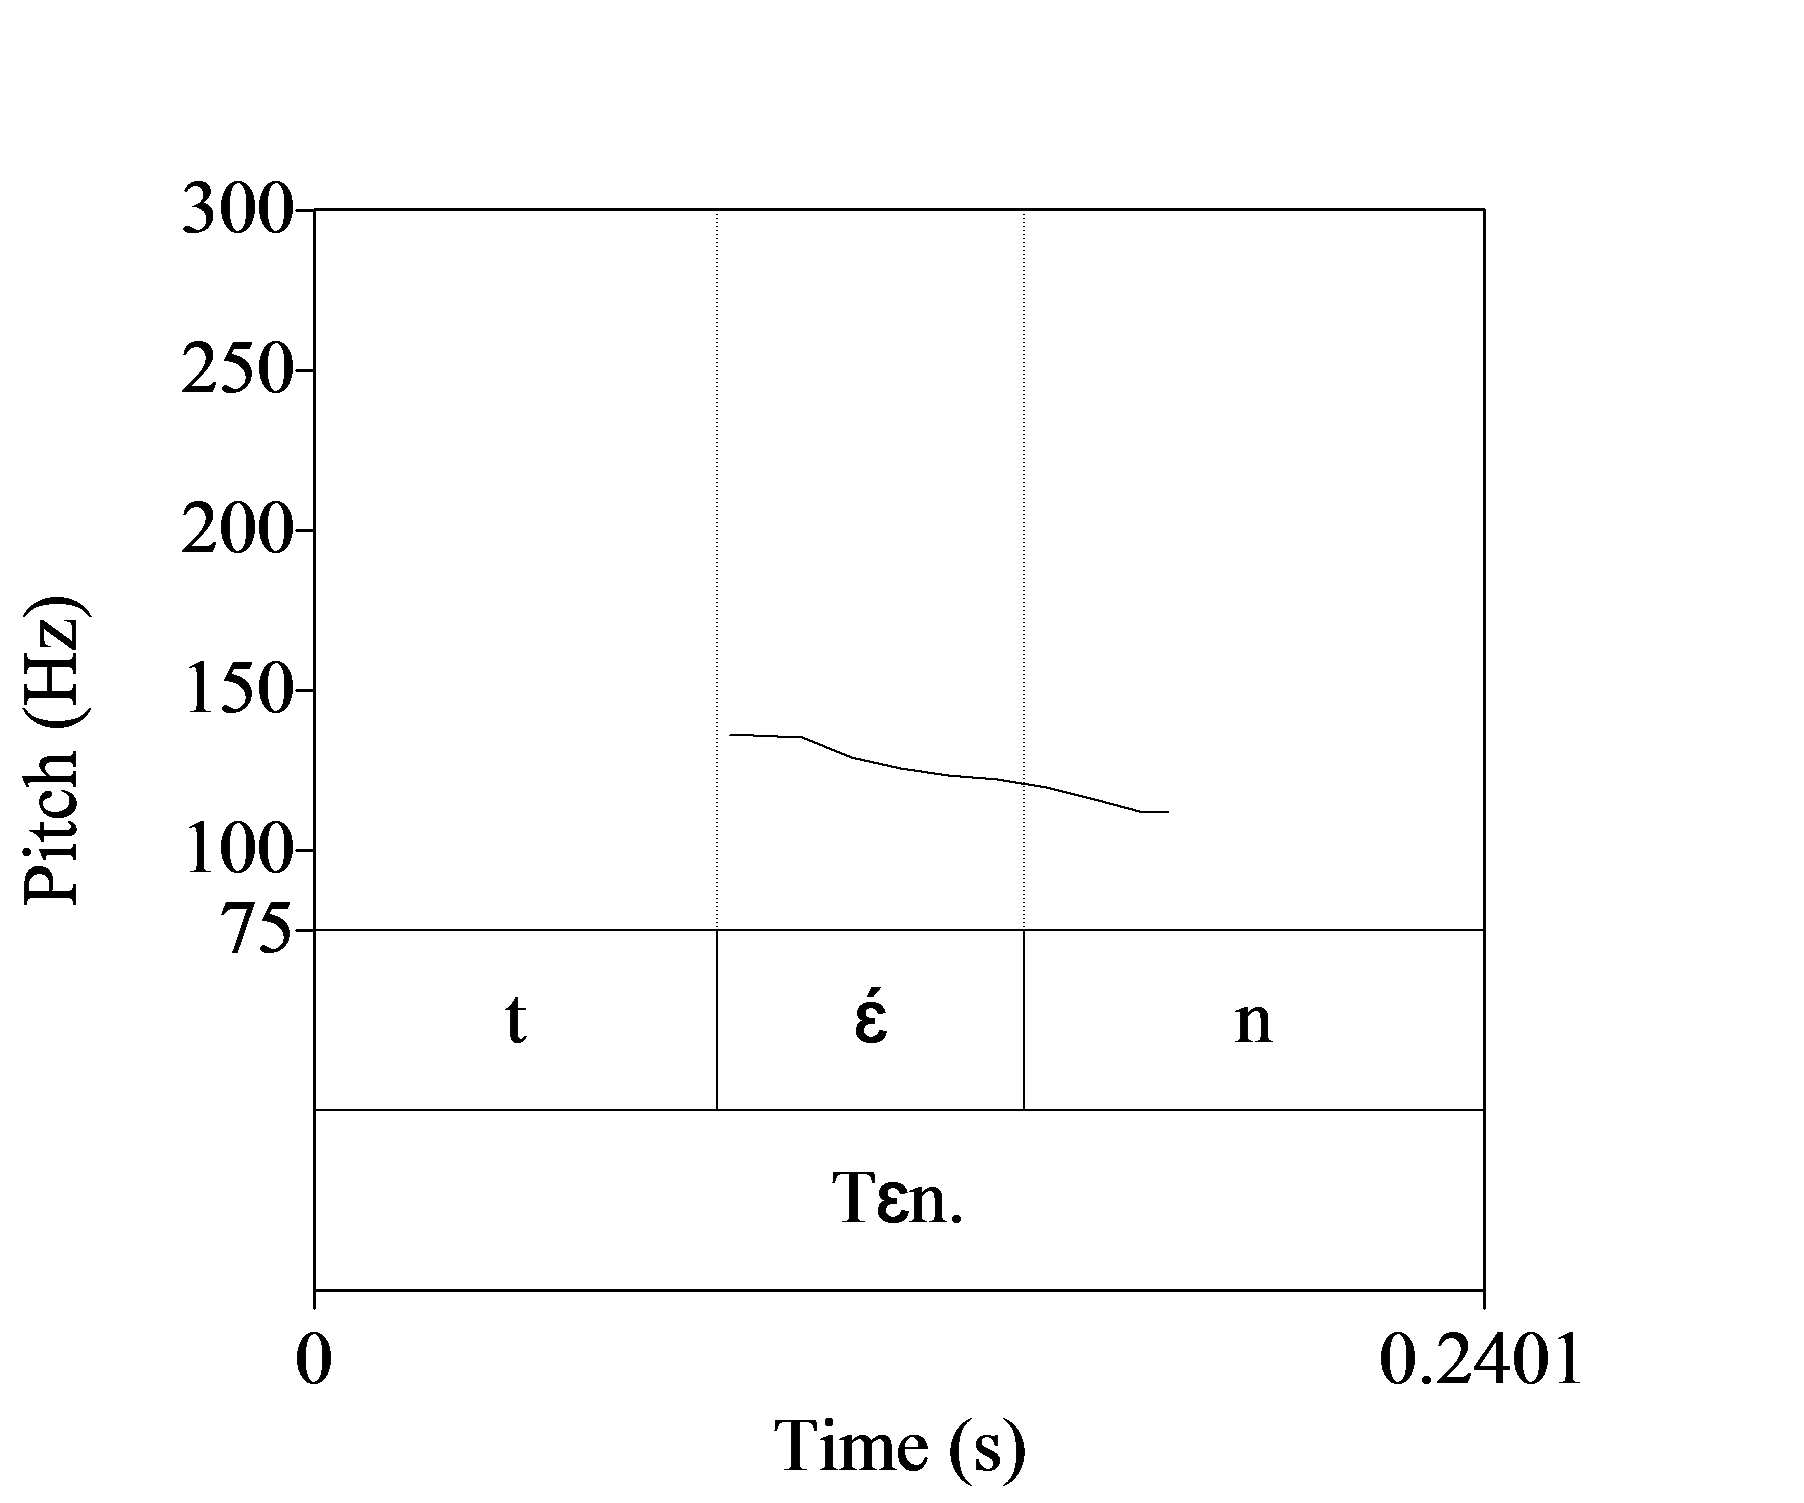
\includegraphics[width=.44\textwidth]{figures/yakpomod-img3.png}
	\label{fig:key:3.1}
\end{figure}
\ea\label{ex:key:43}
\gll Tɛ́n.\\
\textsc{hl\%}\\
\glt  ‘Time’
\z
%}
%\end{minipage}

%\begin{minipage}{.45\textwidth}
%\parbox{.45\textwidth}{
\begin{figure}
	\caption{Citation form of \textstyleTablePichiZchn{tɔ́k}}
	\label{fig:key:3.2}
	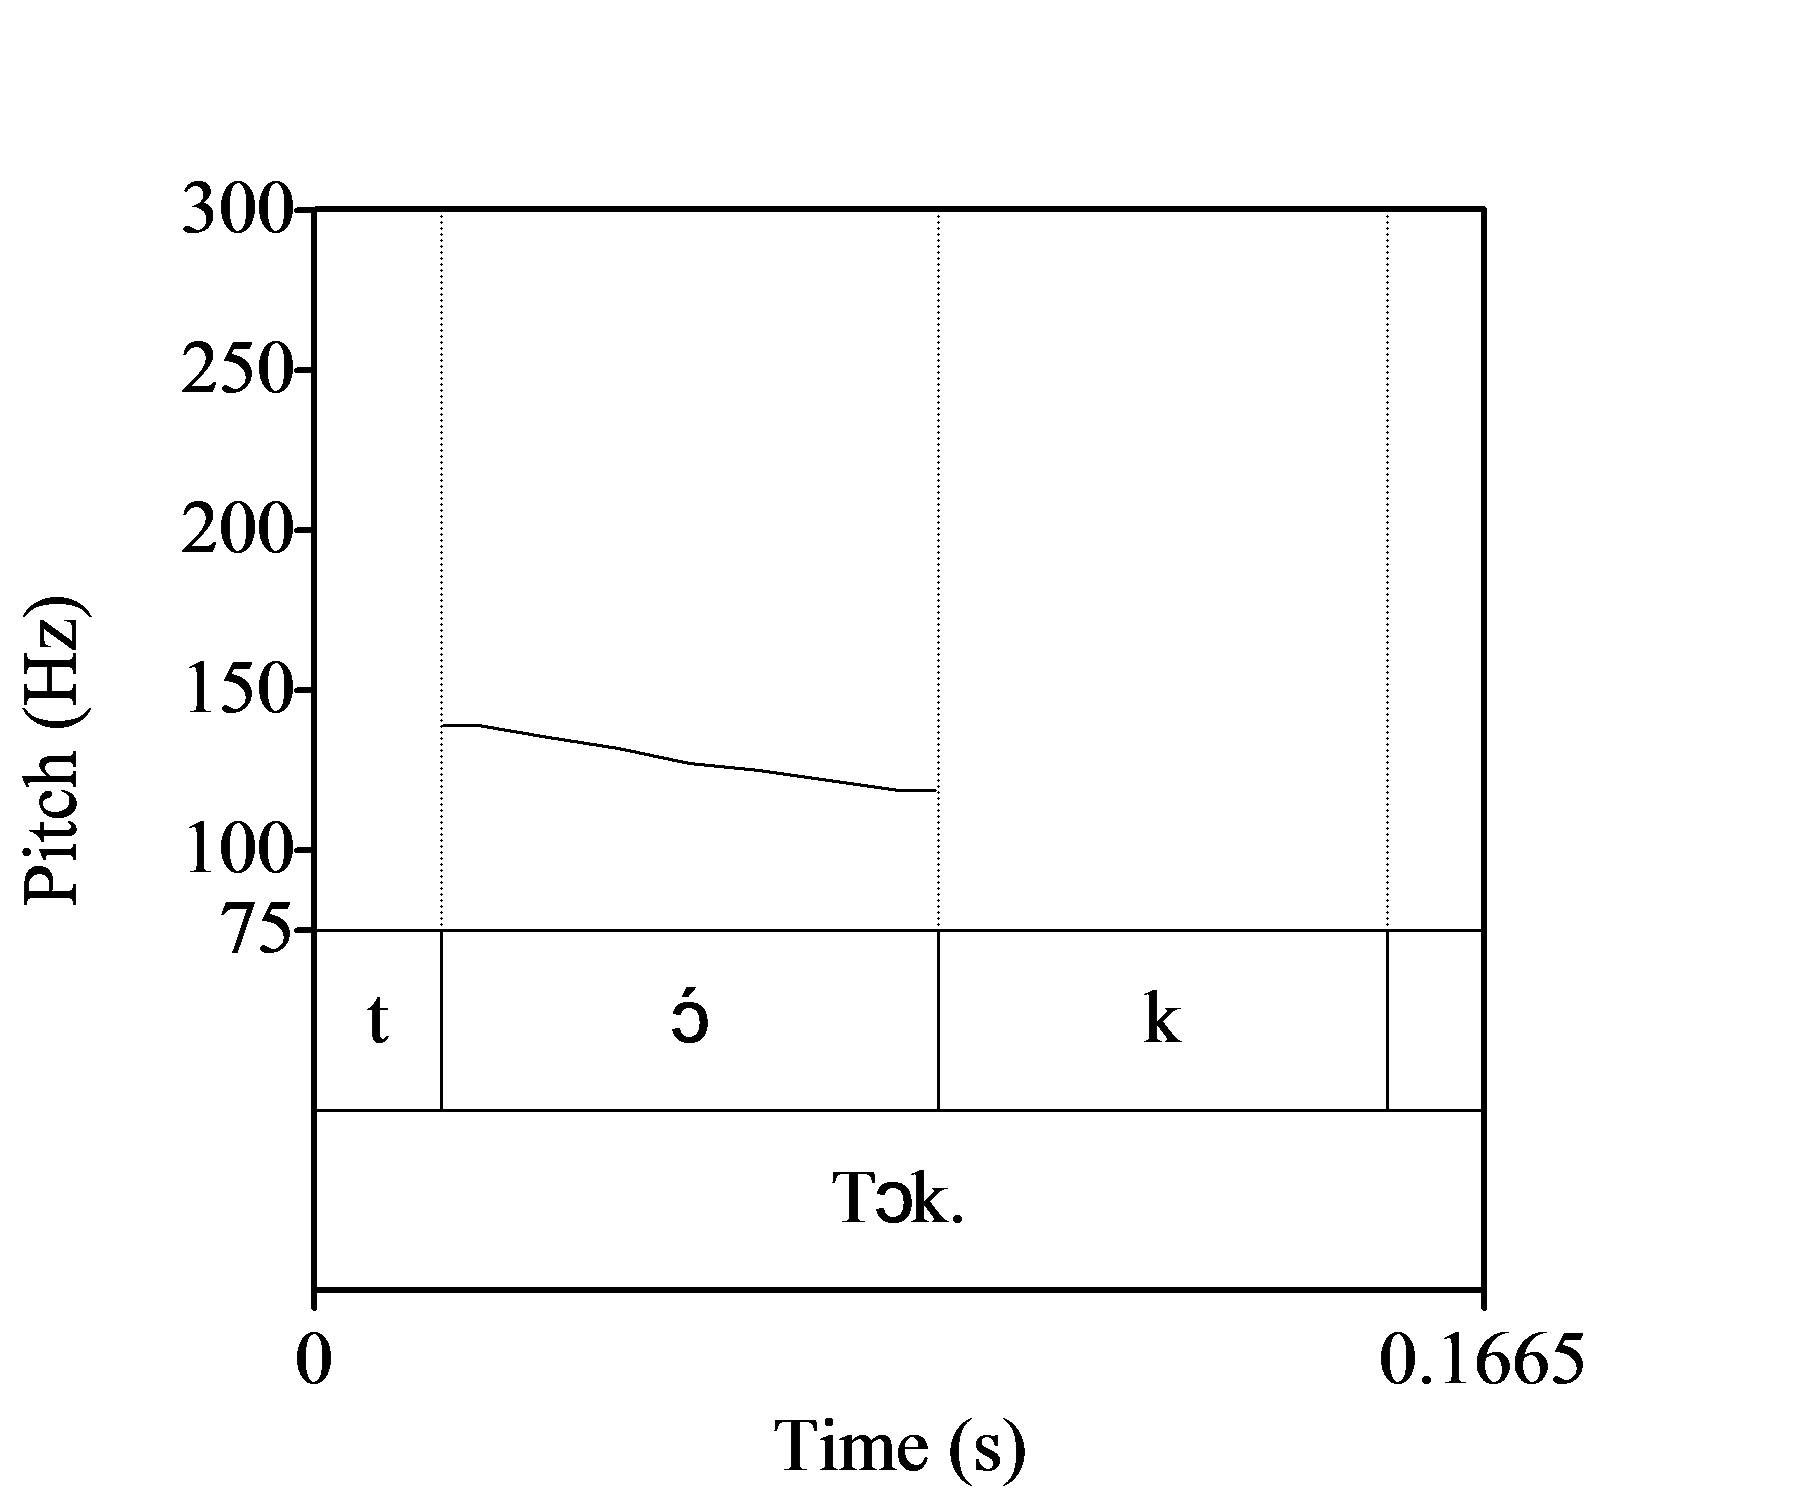
\includegraphics[width=.44\textwidth]{figures/yakpomod-img4.png}
\end{figure}
\ea\label{ex:key:44}
\gll Tɔ́k.\\
\textsc{hl\%}\\
\glt ‘Talk’
\z
%}
%\end{minipage}

When the utterance-final word is a light (vowel-final) monosyllable, the vowel may be lengthened, sometimes up to two beats. I assume that the lengthening of light monosyllables is caused by the metric preference of Pichi for footed tonal domains within the word boundary. Heavy monosyllables with a final non-tone-bearing segment like \textit{tɔ́k} ‘talk’ block the creation of footed domains in utterance-final position. But light syllables leave room for this option. The vowels of the light monosyllables in the following two figures have been lengthened in order to accommodate the HL contour consisting of the lexical H tone of the monosyllable and the declarative L\% boundary tone: 

\begin{figure}
\caption{Citation form of \textstyleTablePichiZchn{só}}
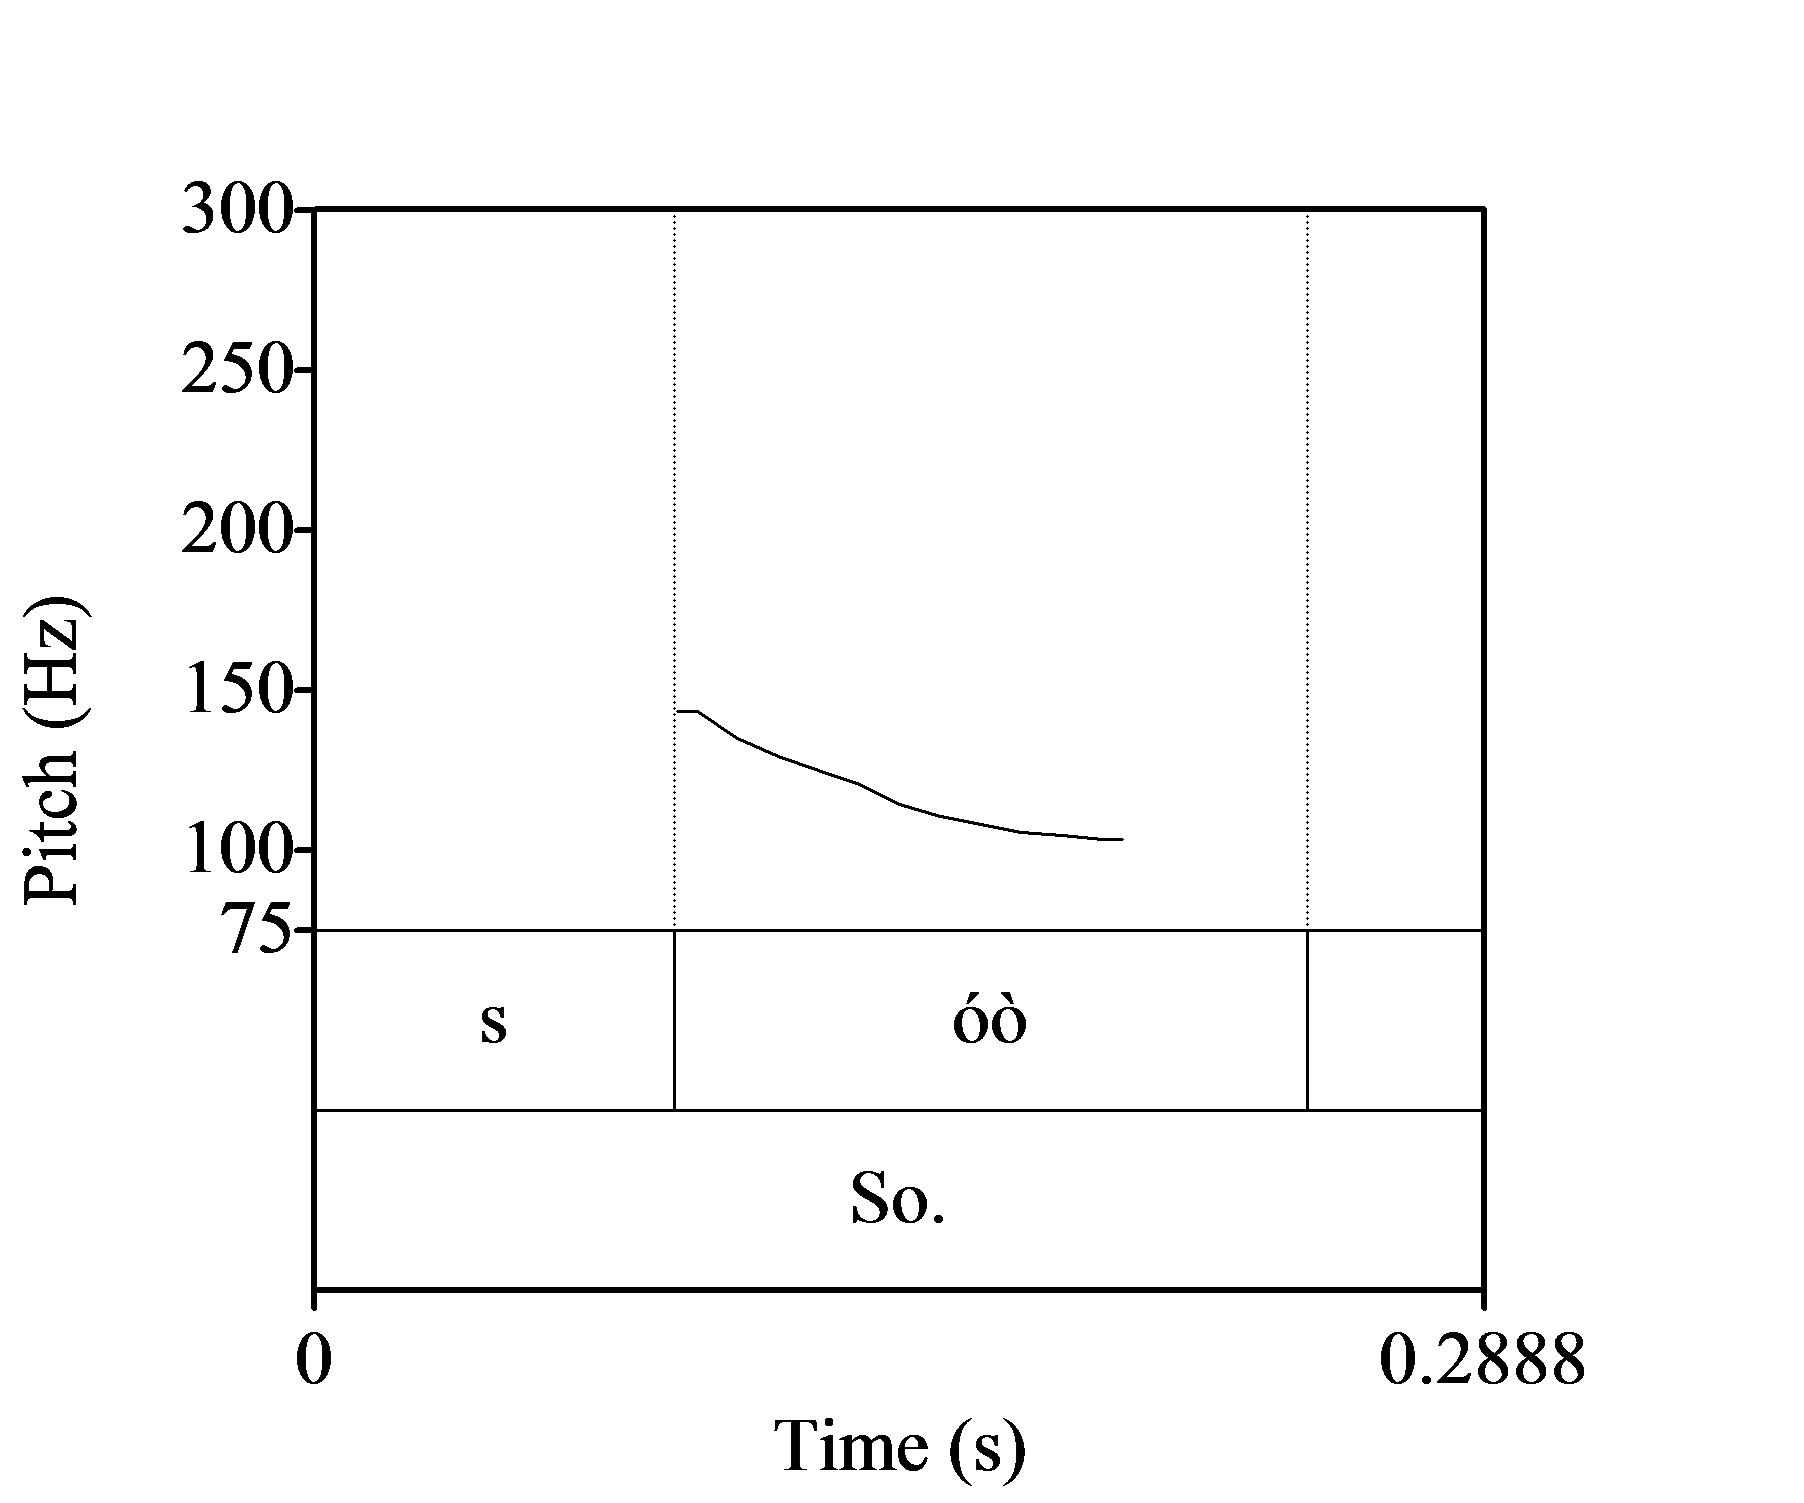
\includegraphics[height=.3\textheight]{figures/yakpomod-img5.png}
\label{fig:key:3.3}
\end{figure}

\begin{figure}
\caption{Citation form of \textstyleTablePichiZchn{dé}}
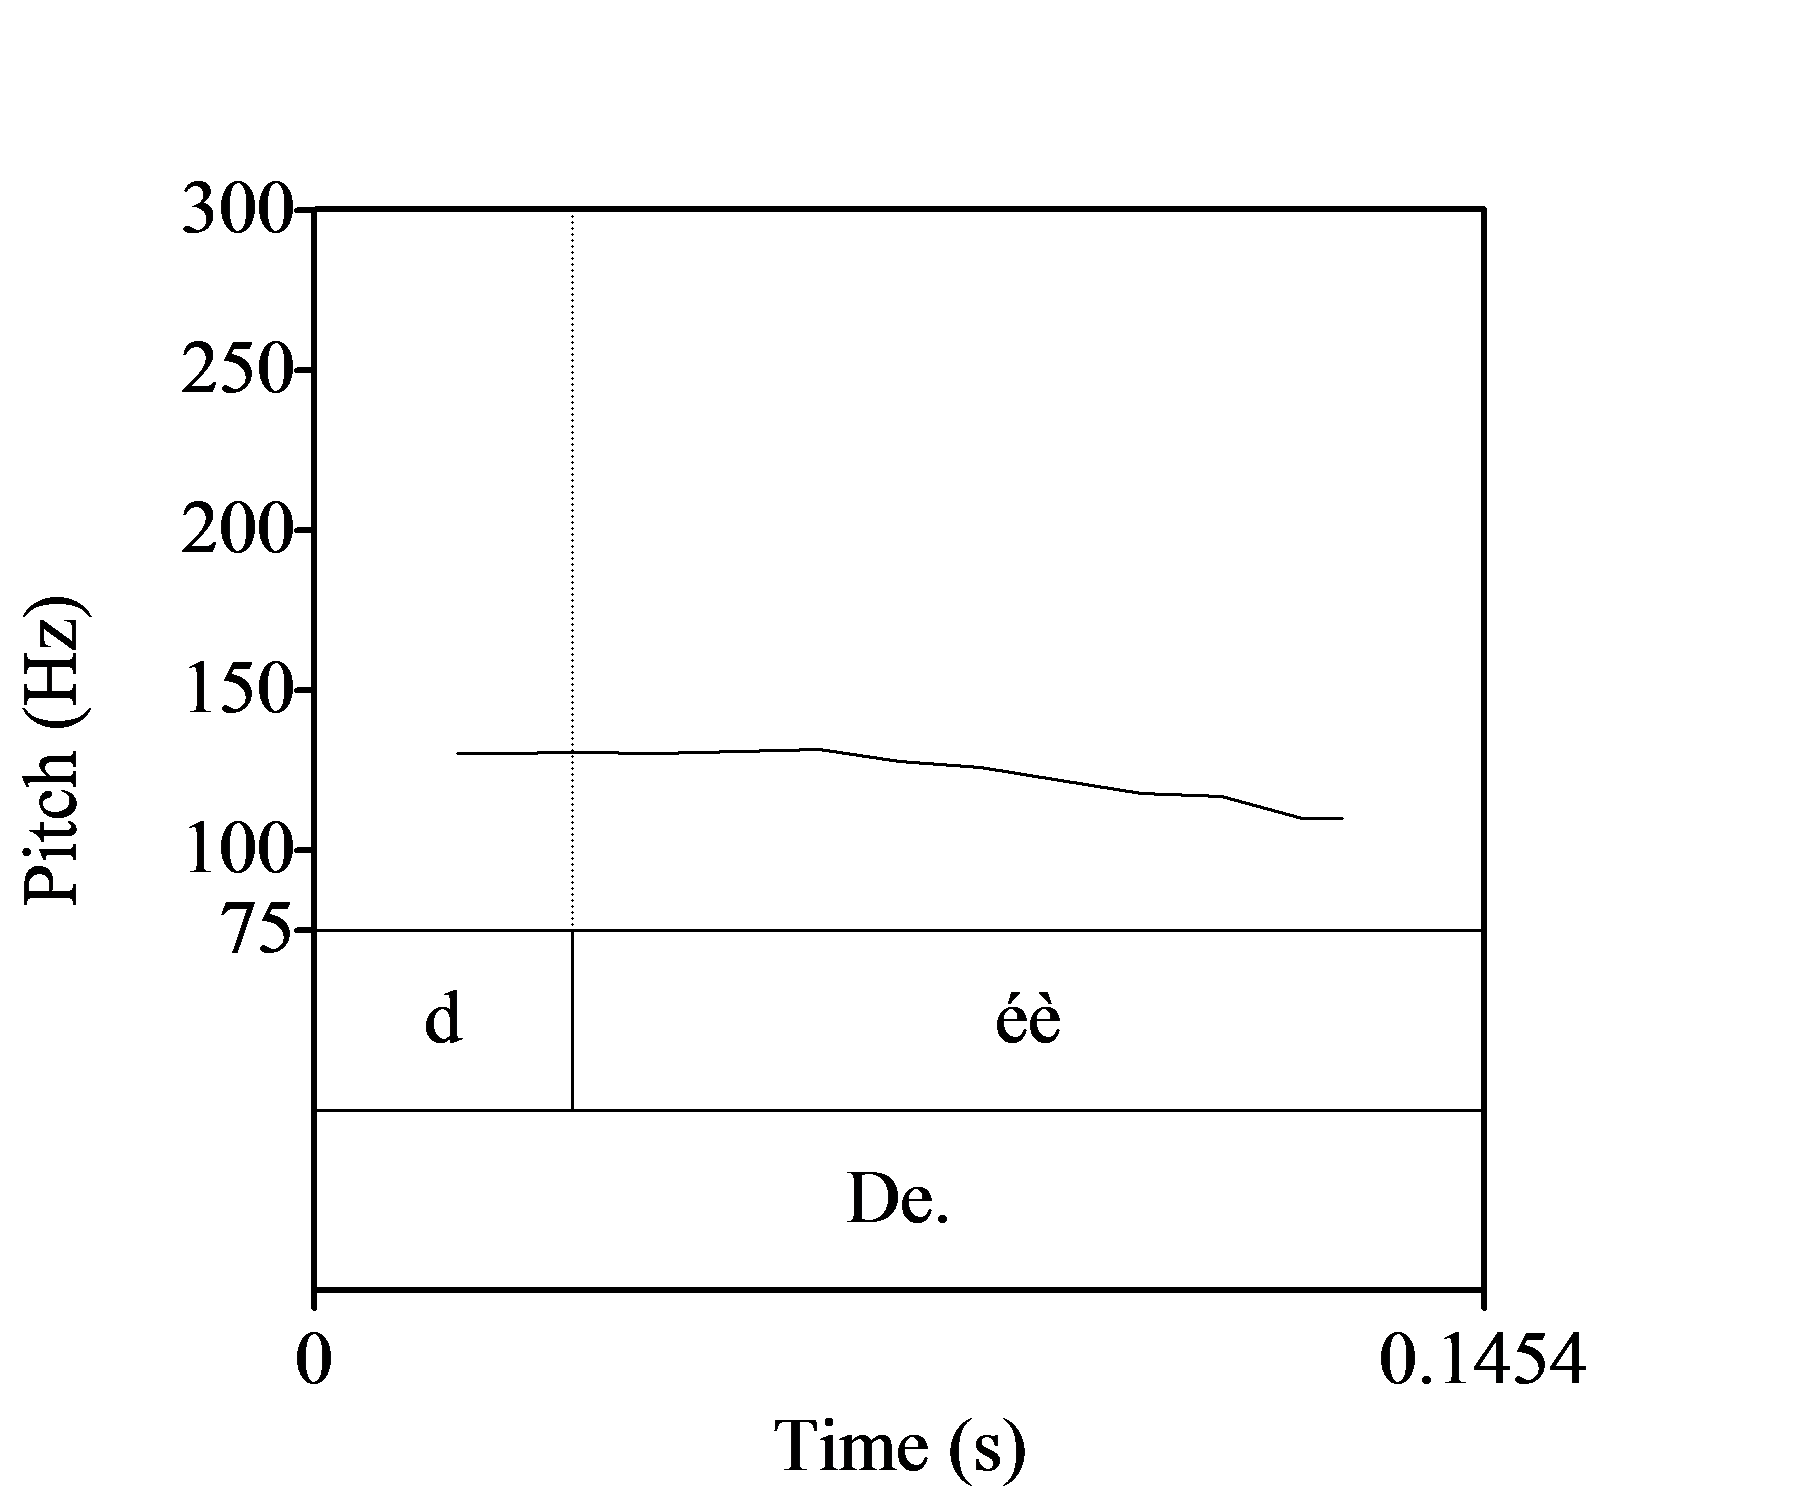
\includegraphics[height=.3\textheight]{figures/yakpomod-img6.png}
\label{fig:key:3.4} 
\end{figure} 

\ea\label{ex:key:45}
\gll      S\textstylePichiexamplebold{ó}.\\
\textsc{h}\textstylePichiexamplebold{\textsc{l\%}}\\
\glt ‘Like that.’
\z
\ea\label{ex:key:46}
\gll    D\textstylePichiexamplebold{é}.\\
\textsc{h}\textstylePichiexamplebold{\textsc{l\%}}\\
\glt ‘There.’
\z

\subsection{Distinctive tones}

Pichi contrasts two level tones, a high tone (H) and a low tone (L). H tone is the more active tone in tonal processes. H rather than L participates in tone spreading and is more active in pitch register expansion. Contour tones do not constitute tonemes in their own right. Instead, they result from the succession of a lexical tone and a polar floating tone over a single tone-bearing unit (cf. \sectref{sec:3.2.2}). 

\figref{fig:key:3.5} and \figref{fig:key:3.6} below present the pitch trace and segmentation of the two words \textit{hasis} /H.L/ ‘ashes’ and \textit{dɔtí} /L.H/ ‘be dirty’ said in isolation:

\begin{figure}
\caption{H.L pattern}
\label{fig:key:3.5}
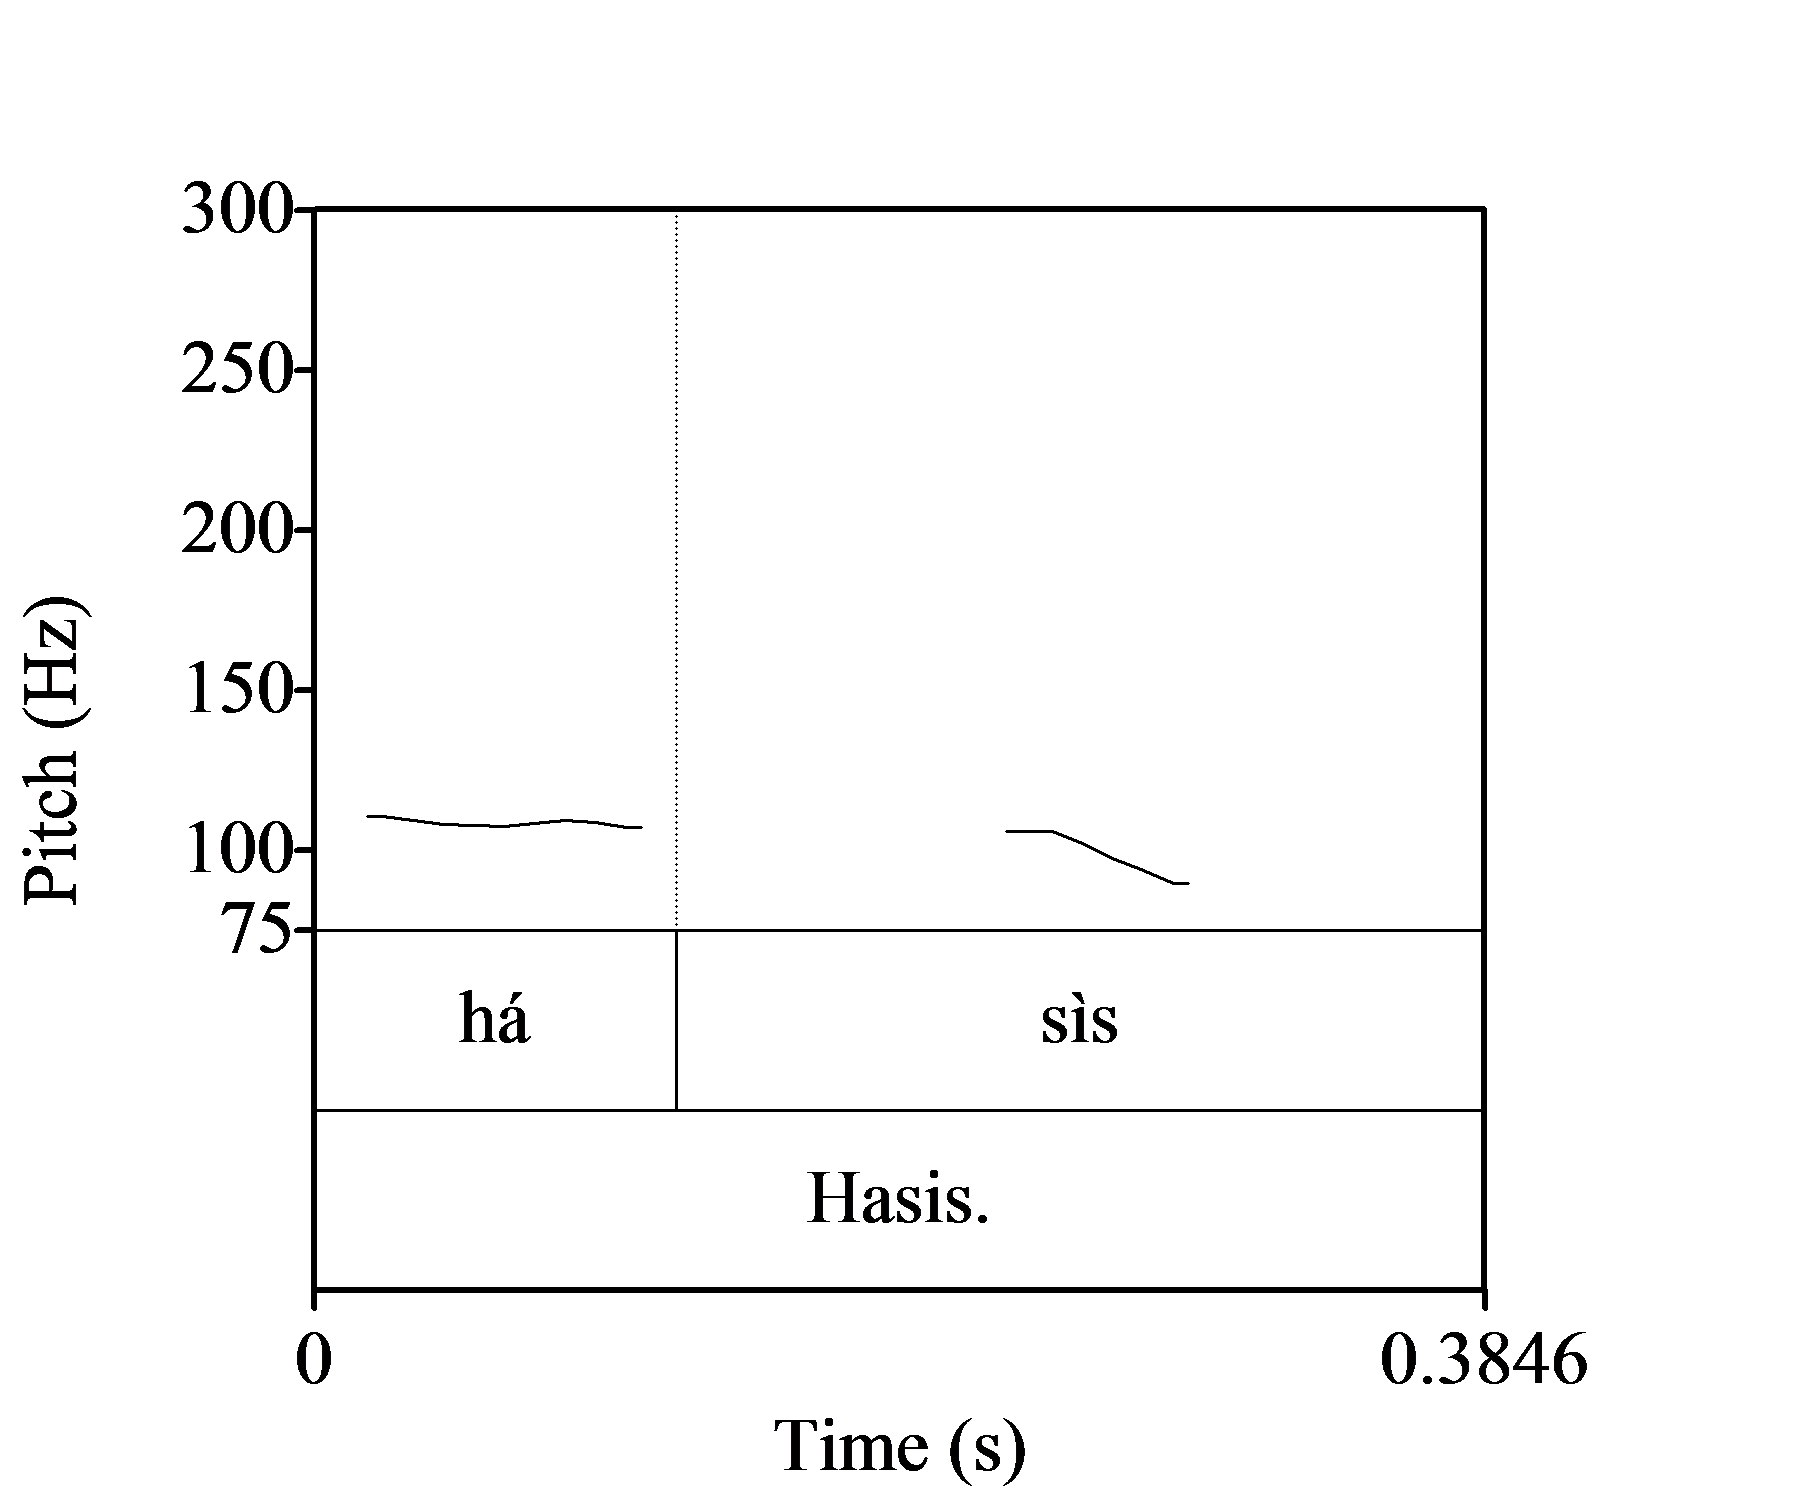
\includegraphics[height=.3\textheight]{figures/yakpomod-img7.png}
\end{figure}

\begin{figure}
\caption{L.H pattern}
\label{fig:key:3.6}  
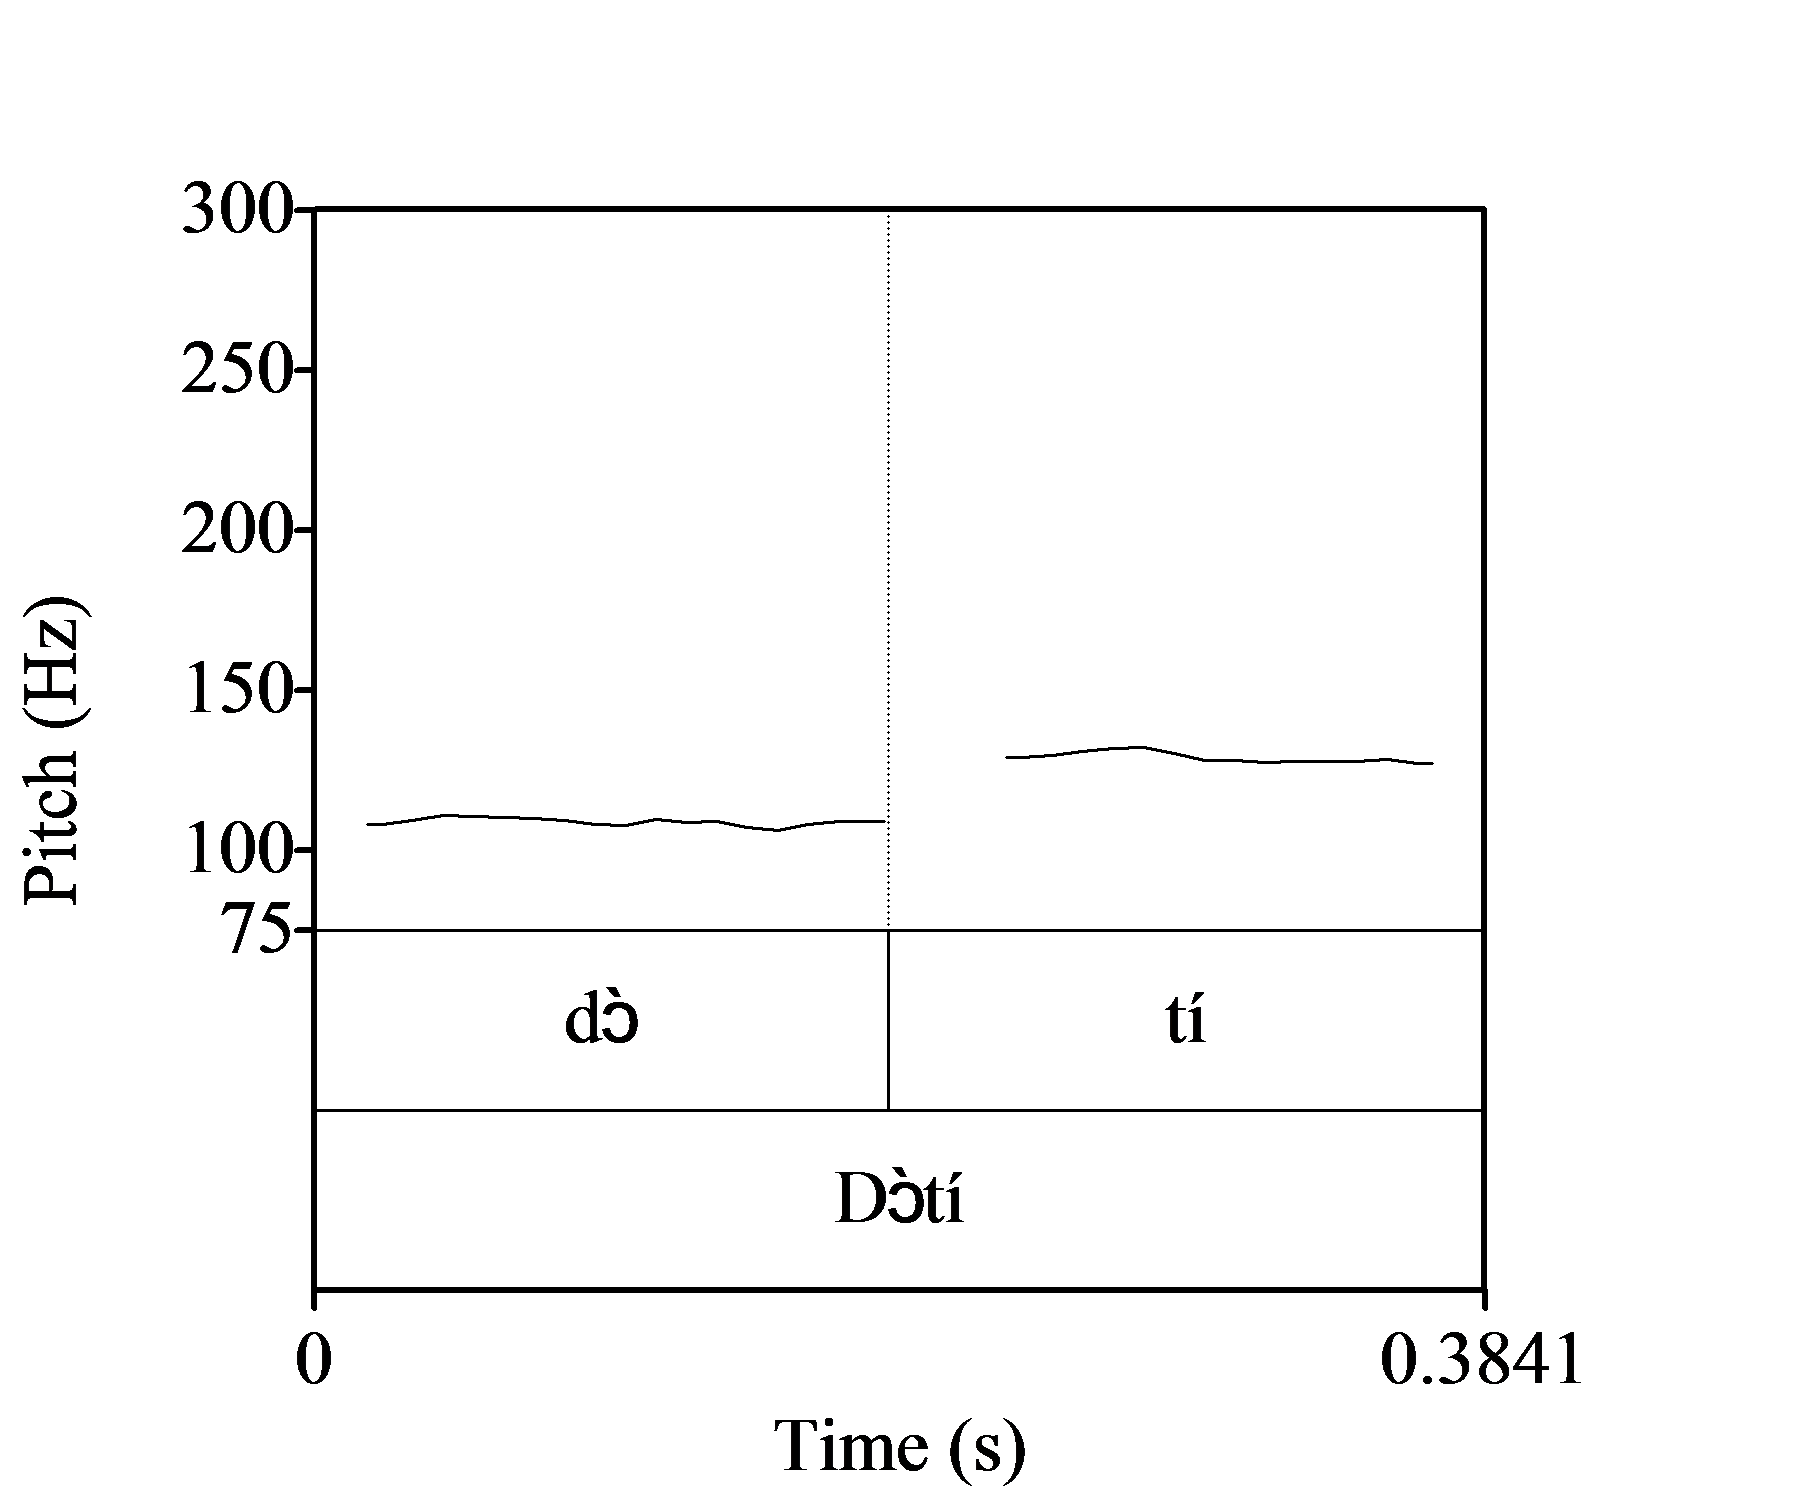
\includegraphics[height=.3\textheight]{figures/yakpomod-img8.png}
\end{figure}

The two words above represent the tone patterns of the two most frequent tone classes of Pichi (cf. \tabref{tab:key:3.1}). The mean pitch on the L-toned syllable of \textit{dɔtí} is 109.17~Hz, that of the H-toned syllable 129.27~Hz. Hence, the difference in pitch between the H- and L-level tones amounts to 20.1~Hz. With \textit{hásis}, the mean pitch of the H tone is 108.59~Hz, while the mean L tone stands at 99.72~Hz. The difference in mean pitch between H and L therefore stands at 8.87~Hz. This difference is just about half of that between L and H in \textit{dɔtí}:

%%please move \begin{table} just above \begin{tabular
\begin{table}
\caption{Pitch values}
\label{tab:key:3.1}

\begin{tabularx}{.5\textwidth}{Xrr}
\lsptoprule
Hertz & \itshape dɔtí & \itshape hásis\\
\midrule
Mean Hz of H    & 129.27 & 108.59\\
Mean Hz of L    & 109.17 & 99.72\\
Highest Hz of H & 132.20 & 110.33\\
Lowest Hz of H  & 127.26 & 107.35\\
Highest Hz of L & 110.78 & 105.83\\
Lowest Hz of L  & 107.47 & 93.50\\
\lspbottomrule
\end{tabularx}
\end{table}
The relatively small difference in mean pitch between the syllables of \textit{hásis} arises due to the fact that the H tone over the first syllable is carried over into the first half of the following L-toned syllable. In contrast, the L tone of the first syllable of \textit{dɔtí} shows no signs of rightward spreading. 


Words may bear a single or more H or L tones. Compare the pitch traces of the utterance-final tonal words nyɔ́ní ‘ant’ and Bata ‘Fang’ in the collocations lɛ́k nyɔ́ní ‘like ants’ and tɔ́k Bata ‘speak Fang’ below:


\begin{figure}
\caption{H.H pattern} 
\label{fig:key:3.7}
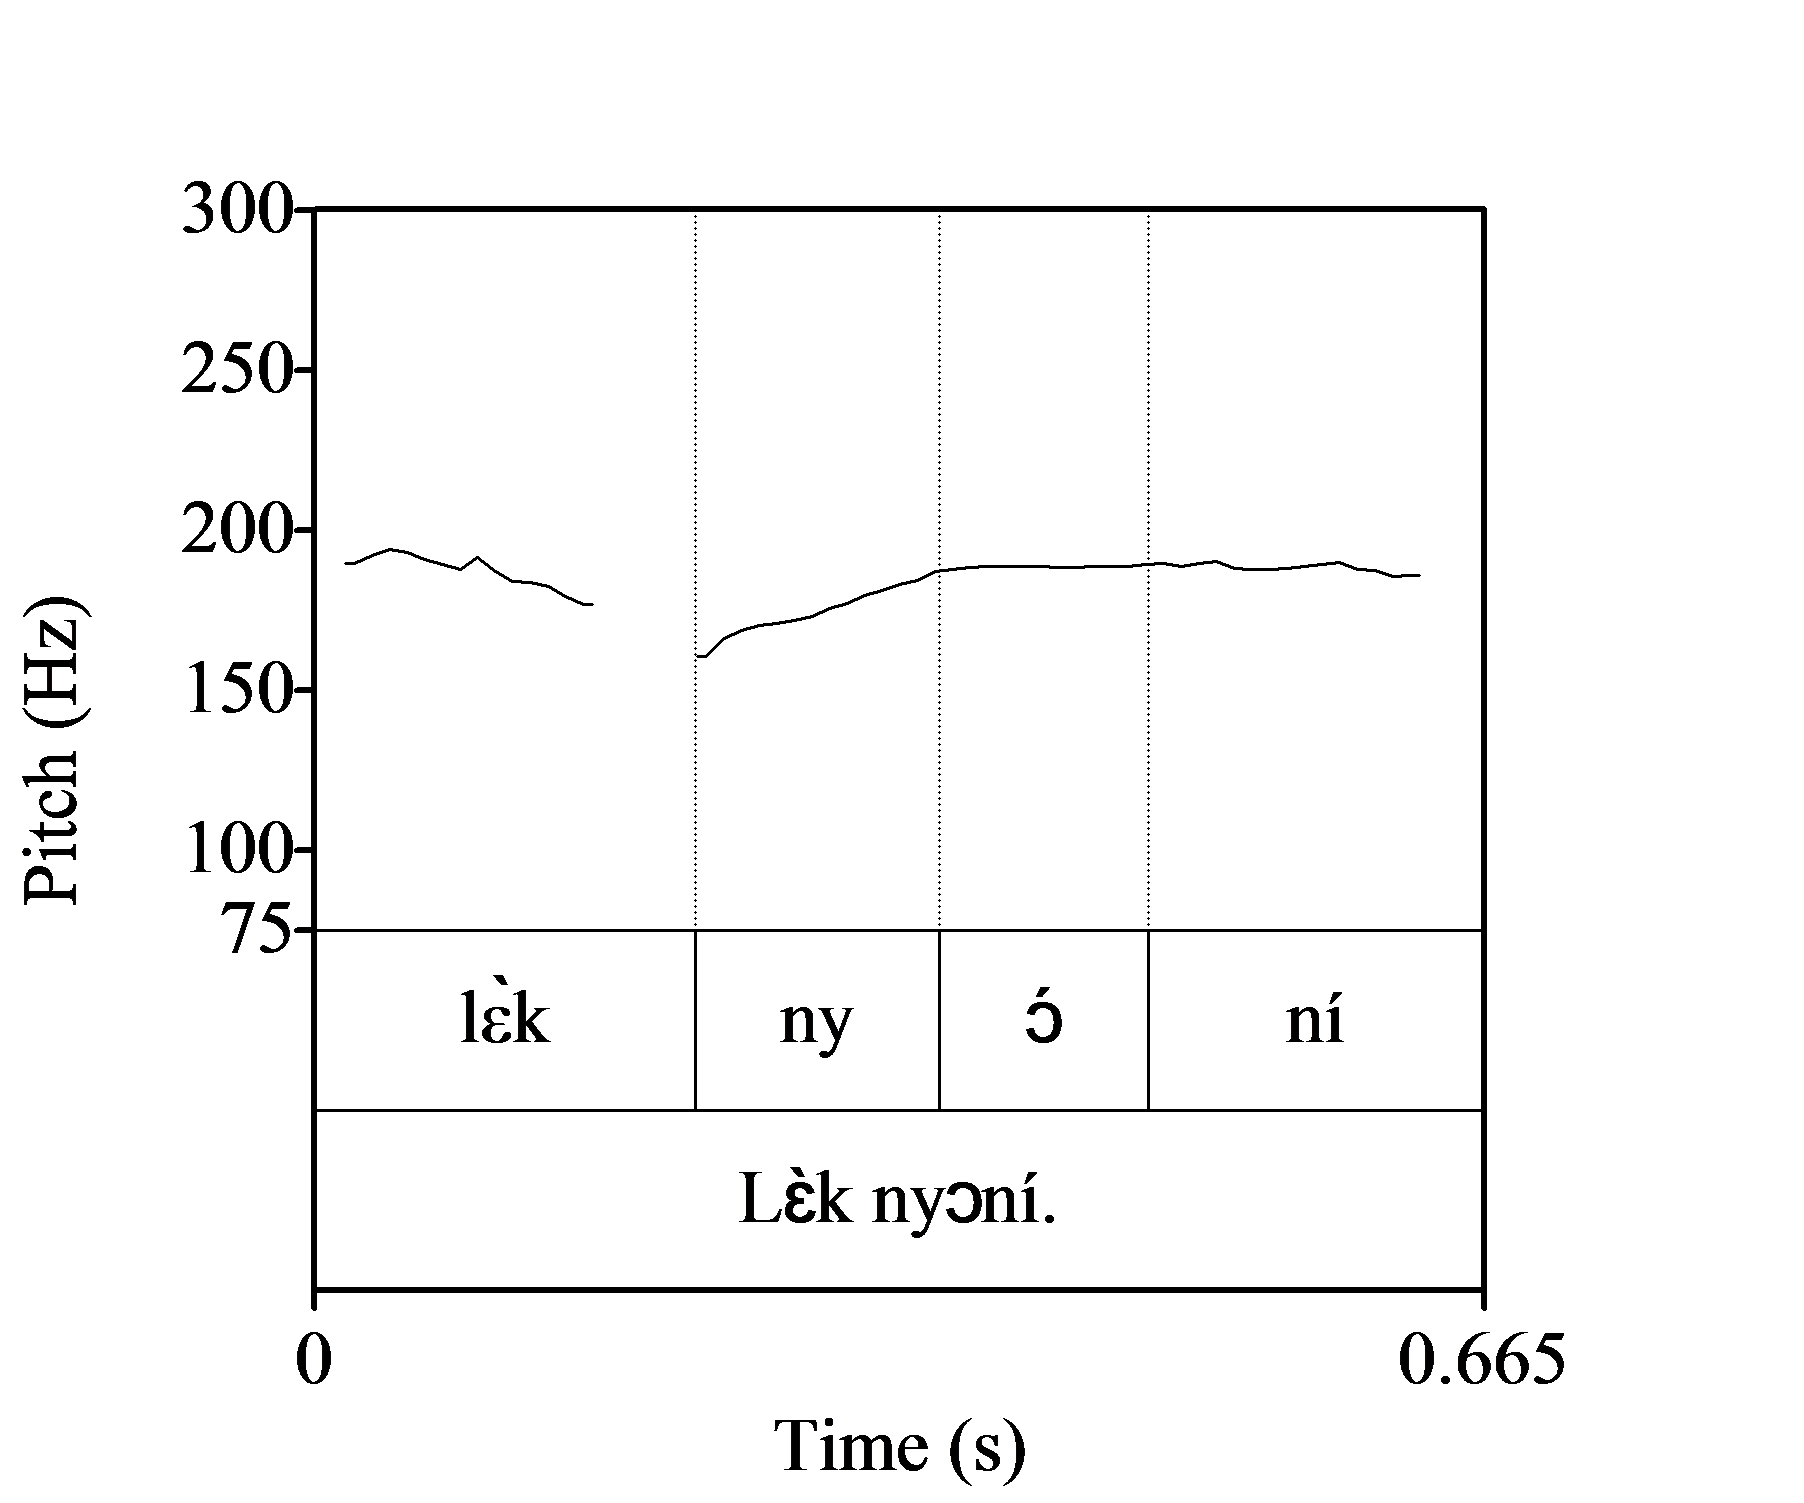
\includegraphics[height=.3\textheight]{figures/yakpomod-img9.png}
\end{figure}

\begin{figure}
\label{fig:key:3.8}
\caption{L.L pattern}
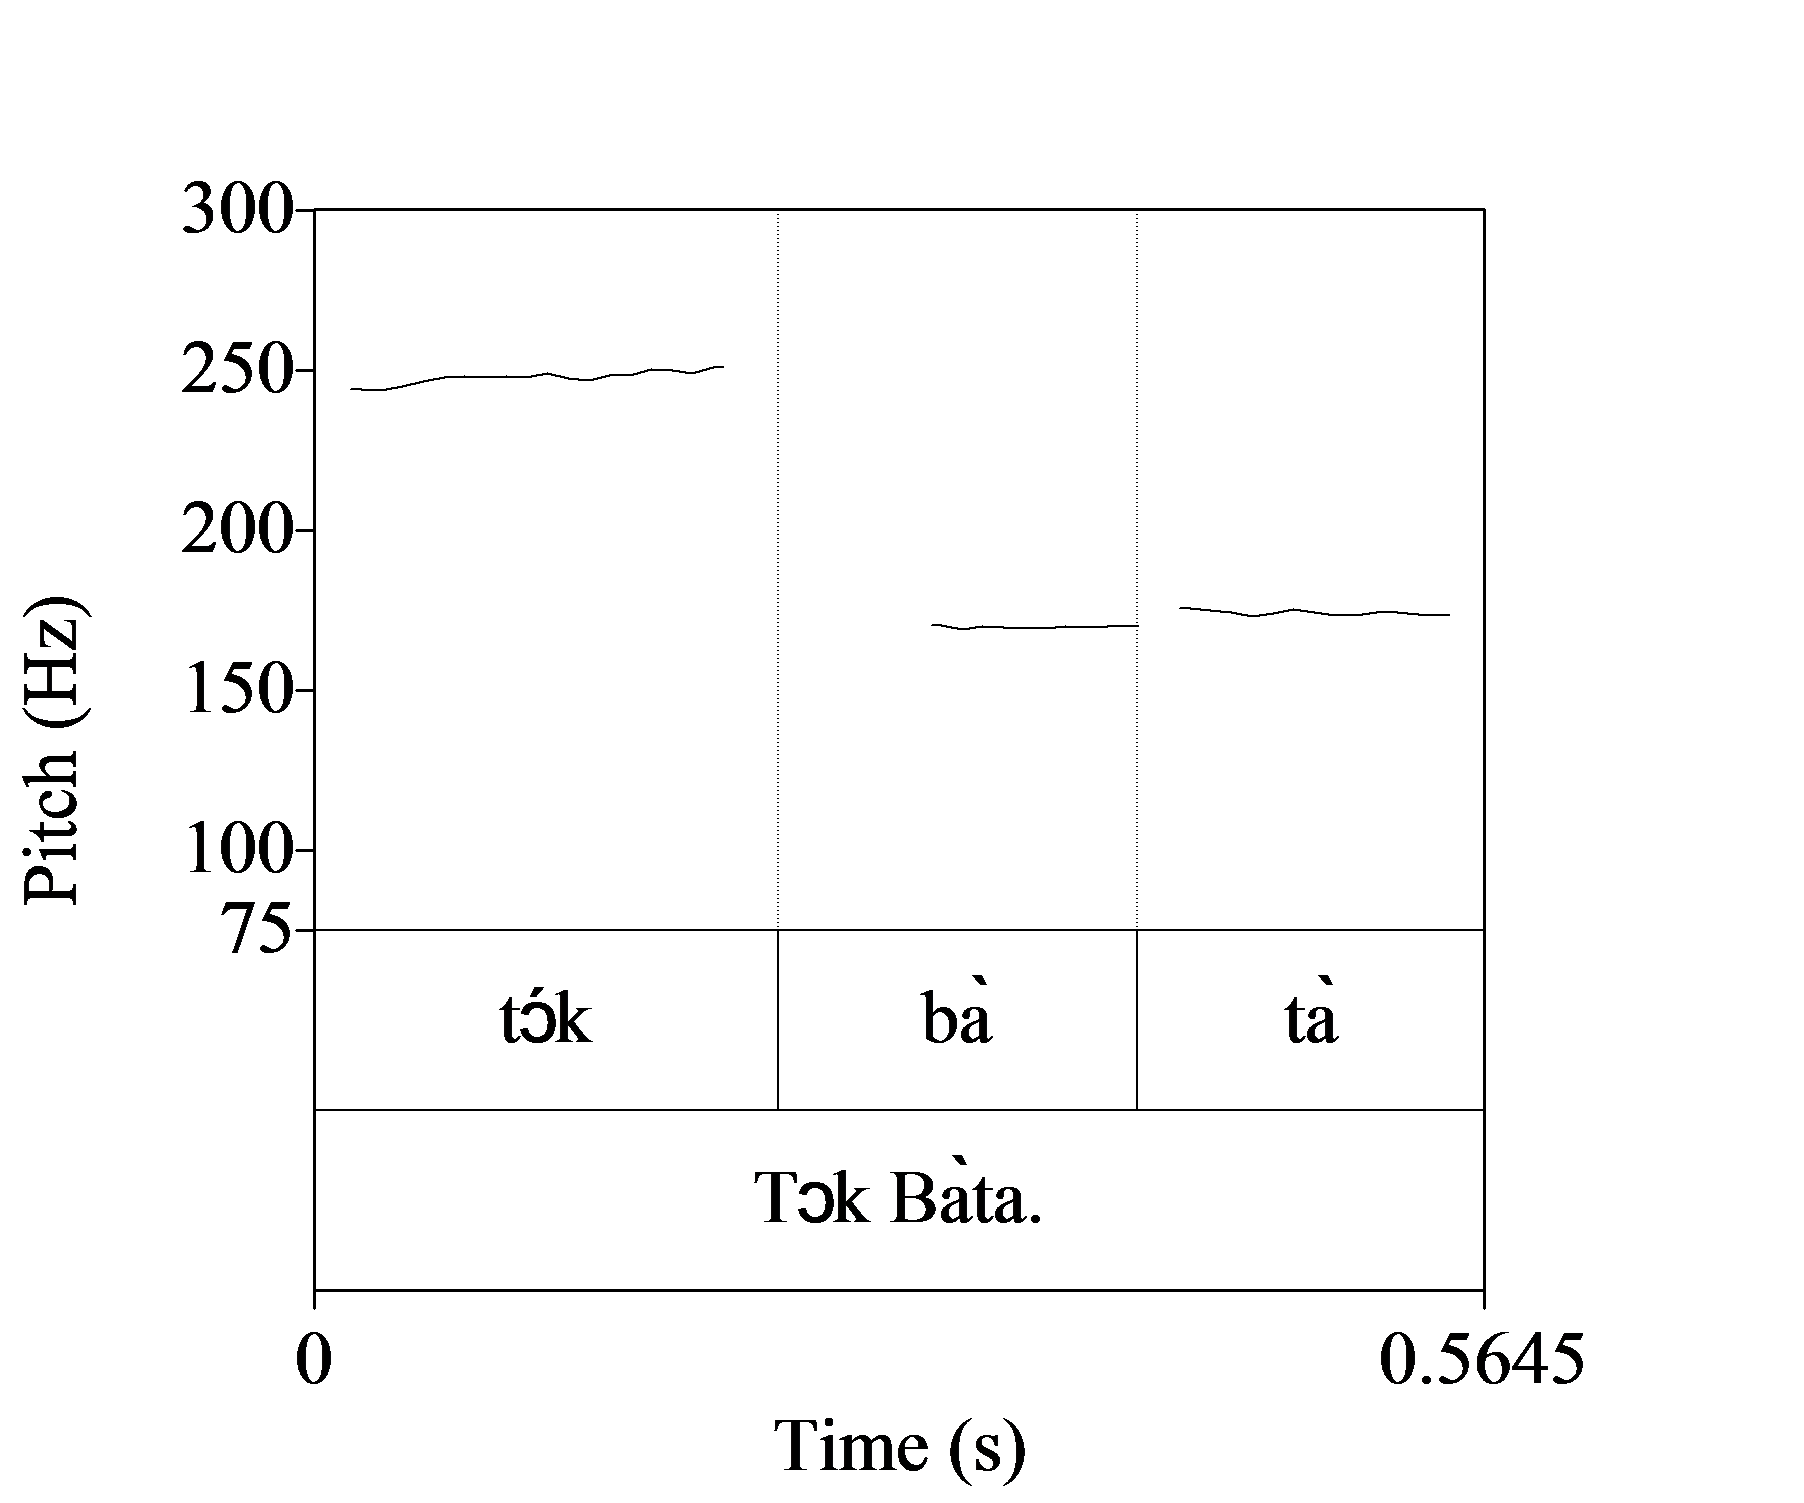
\includegraphics[height=.3\textheight]{figures/yakpomod-img10.png}
\end{figure}

Equatoguinean Spanish has been analysed as a tone language, in which the lexical stress characteristic of Spanish has been converted to lexical tone due to contact with the tone languages of Equatorial Guinea (\citealt{Lipski2015,SteienYakpo2017}). Words code-switched or borrowed from Equatoguinean Spanish are therefore specified for lexical tone just like Pichi words. 


The two tables below feature the utterance-final Spanish words \textit{abril} ‘April’ and \textit{nigeriano} ‘Nigerian’, the latter in the collocation \textit{na} \textit{nigeriano} ‘\textsc{foc} Nigerian’ \textit{=} ‘He is a Nigerian’. The pitch configurations over these two words conforms to those of Pichi words with a word-final (\figref{fig:key:3.9}) and a penultimate (\figref{fig:key:3.10}) H tone, respectively: 


\begin{figure}
\caption{Pitch over Spanish \textstyleTablePichiZchn{abril}}
\label{fig:key:3.9}
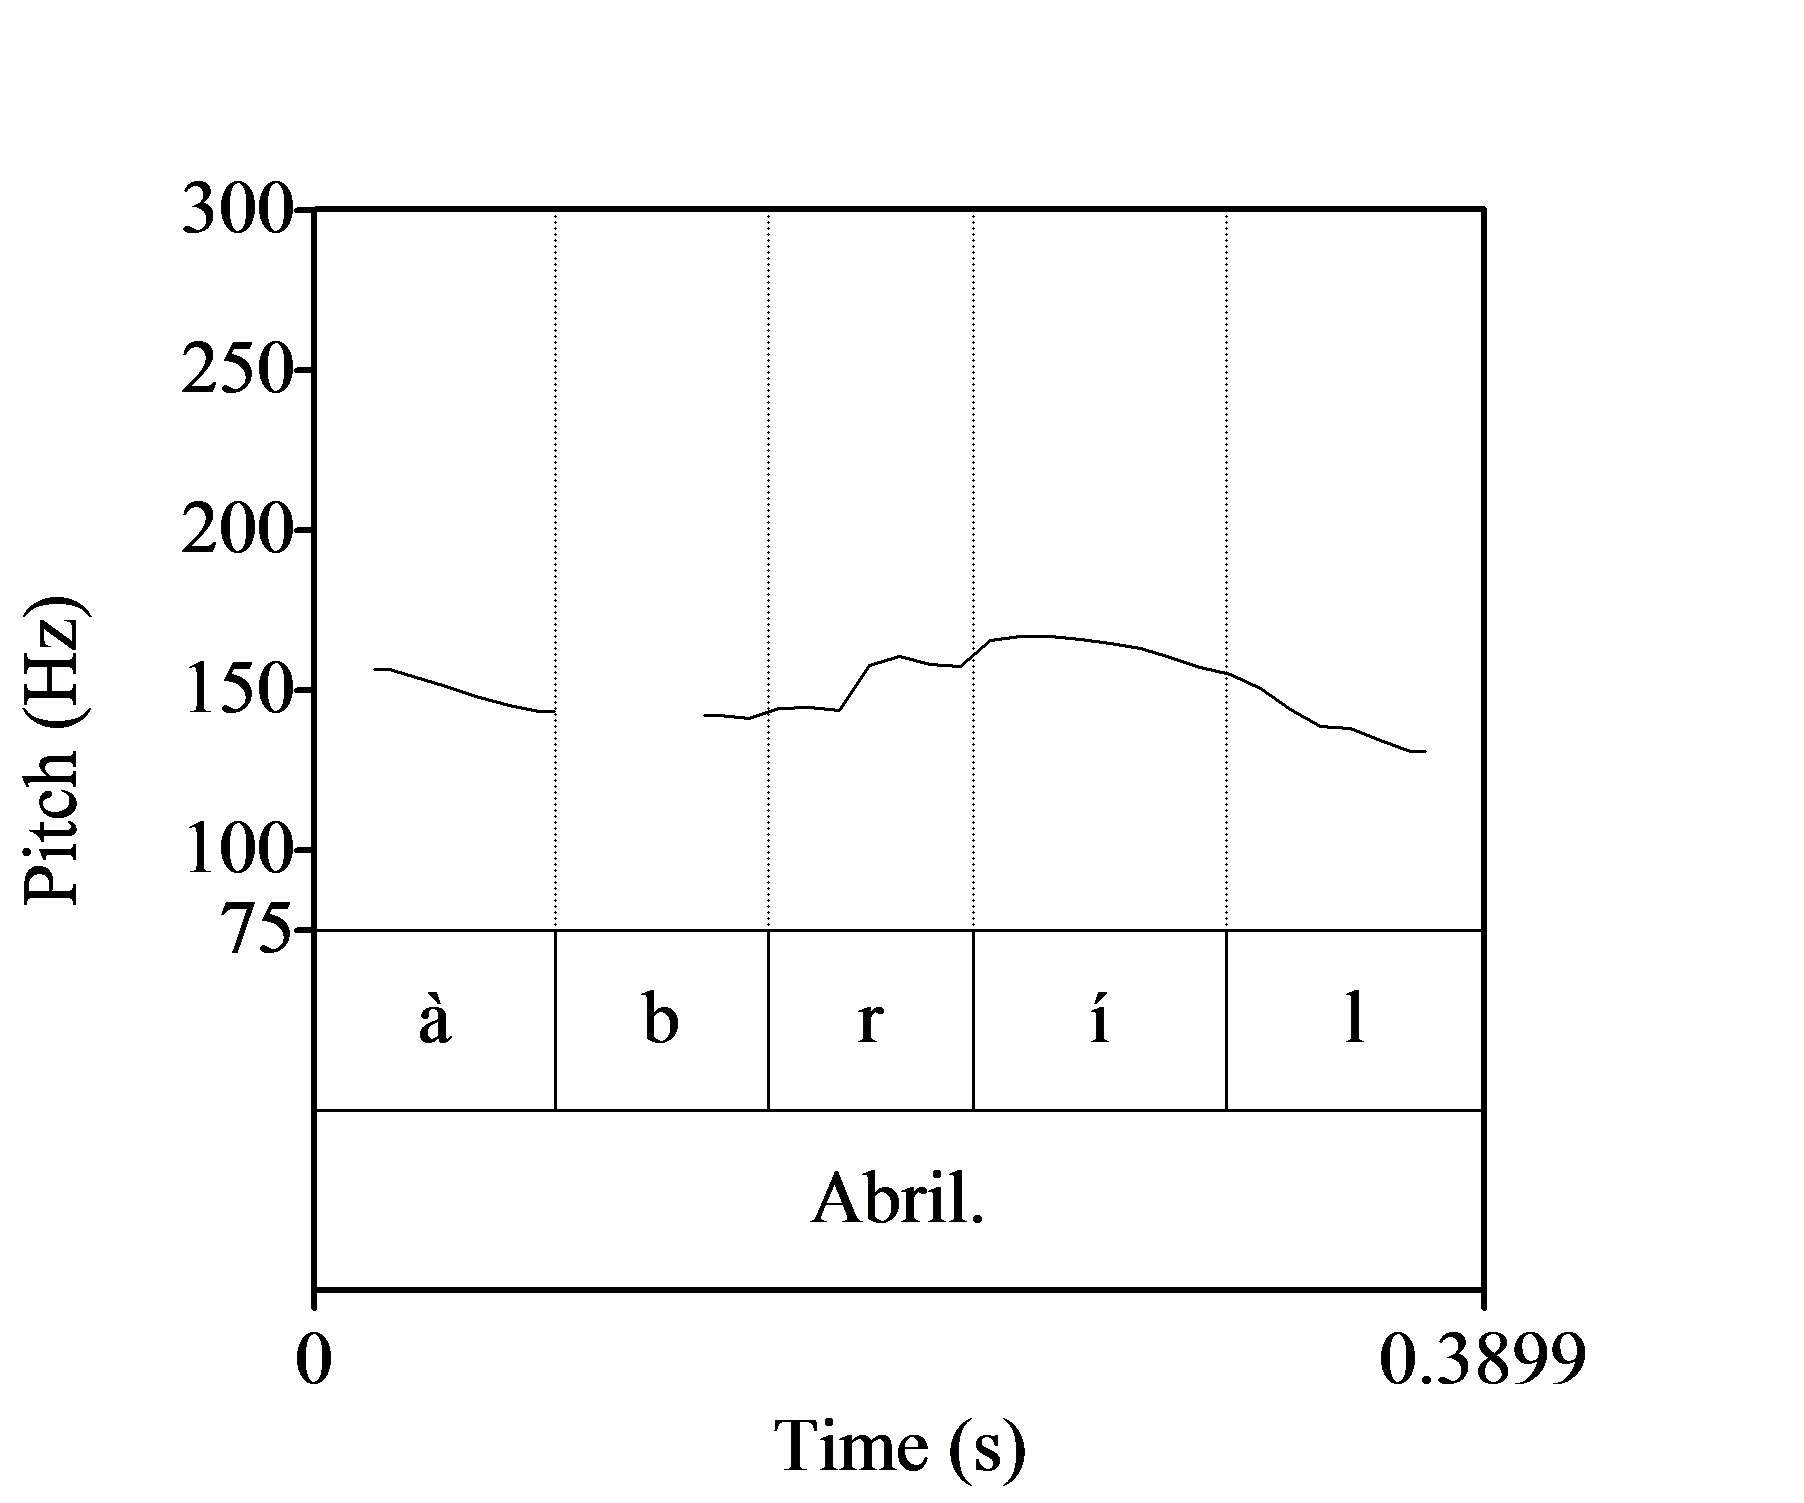
\includegraphics[height=.3\textheight]{figures/yakpomod-img11.png}
\end{figure}

\begin{figure}
\caption{Pitch over Spanish \textit{nigeriano}}
\label{fig:key:3.10} 
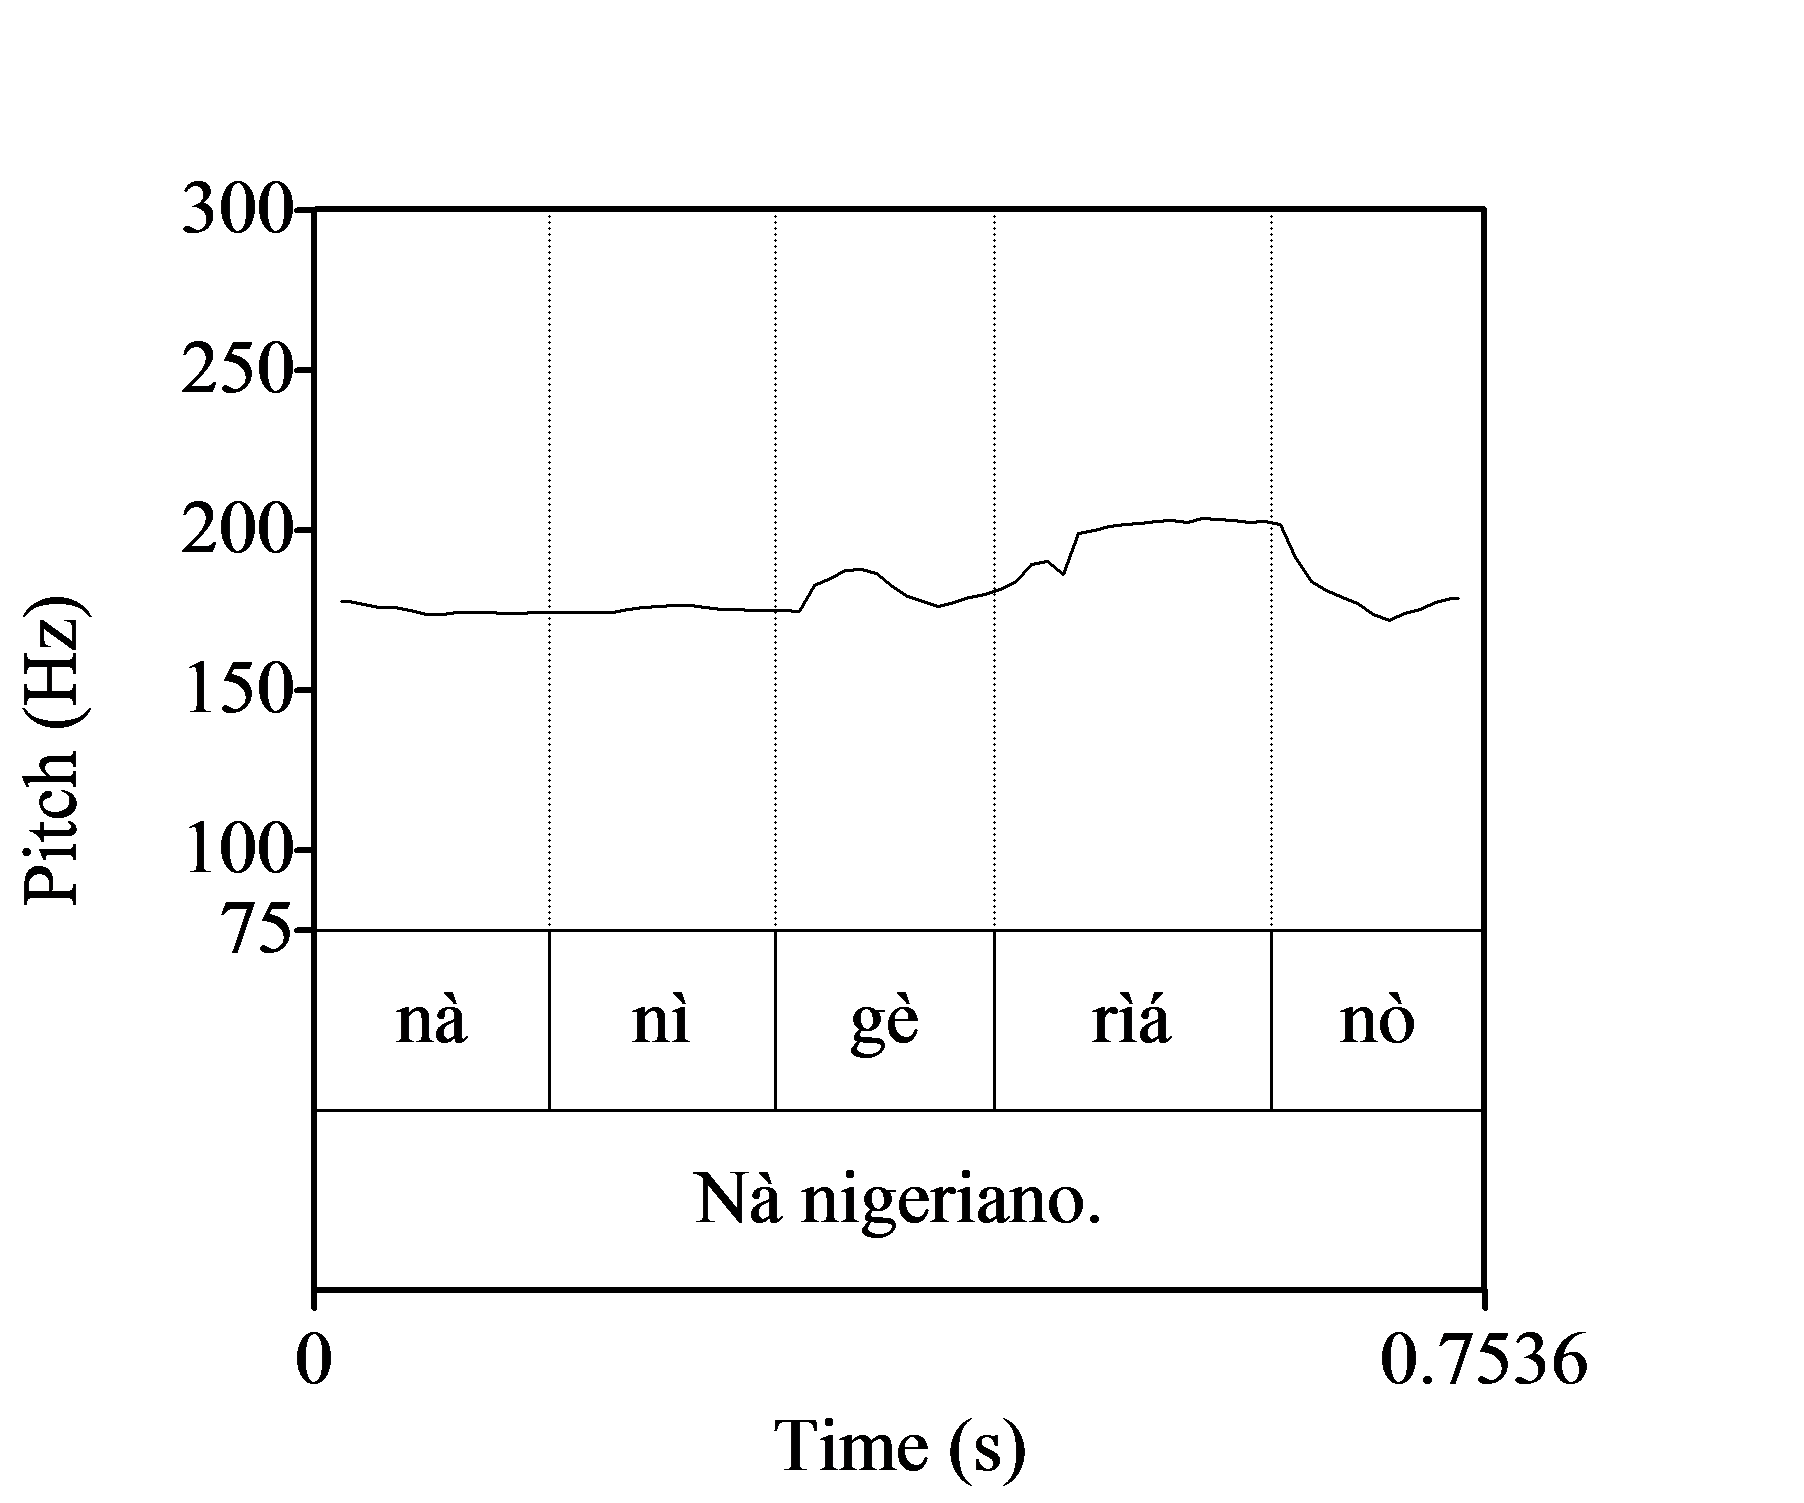
\includegraphics[height=.3\textheight]{figures/yakpomod-img12.png}
\end{figure}

\subsection{Lexical and morphological tone}

A small number of monosyllabic roots are distinguished from each other by pitch alone. The list in \REF{ex:key:47} contains most words in the corpus to which this applies. In conformity with a general pattern, (more) functional words are L-toned, while the corresponding content words are H-toned: 

\eabox{\label{ex:key:47}
\begin{tabularx}{\textwidth}{ll ll}
L tone &  & H tone & \\
\itshape bay & ‘by’ & \itshape báy & ‘buy’\\
\itshape bɔt & ‘but’ & \itshape bɔ́t & ‘hit with the head’\\
\itshape de & ‘\textsc{ipfv}’ & \itshape dé & ‘day; there’\\
\itshape di & ‘\textsc{def}’ & \itshape dí & ‘this’\\
\itshape lɛk & ‘like’ & \itshape lɛ́k & ‘(to) like’\\
\itshape so & ‘so’ & \itshape só & ‘like this; sew; show’\\
\itshape wet & ‘with’ & \itshape wét & ‘wait’\\
\end{tabularx}
}

However, there are also numerous homophones, which can neither be distinguished segmentally, nor by their pitch properties. The following list contains most homophones in the corpus: 

\eabox{\label{ex:key:48}
\begin{tabularx}{\textwidth}{ll ll}
\multicolumn{2}{l}{Homophones} &  & \\
\itshape dé & ‘day; there; \textsc{be.loc}’ & \itshape líf & ‘leaf; live’\\
\itshape an & ‘\textsc{3sg.obj}; and’ & \itshape lɔ́s & ‘loose; louse’\\
\itshape día & ‘deer; expensive’ & \itshape na & \textsc{‘foc;} \textsc{loc’}\\
\itshape bia & ‘beer; bear’ & \itshape nó & ‘know; \textsc{neg’}\\
\itshape bló & ‘blow; relax’ & \itshape nyús & ‘news; use’\\
\itshape fɔ́l & ‘fowl; to rain’ & \itshape pía & ‘avocado; pair’\\
\itshape fɔ́s & ‘first; force’ & \itshape ráyt & ‘right; write’\\
\itshape fíl & ‘feel; field’ & \itshape rɛ́s & ‘rest; rice’\\
\itshape hát & ‘heart; to hurt’ & \itshape rɔ́n & ‘run; be wrong’\\
\itshape hía & ‘hear; here; year; hair’ & \itshape só & ‘sew; show’\\
\itshape hól & ‘hole; hold; whole’ & \itshape sɔ́t & ‘shirt; short’\\
\itshape (h)ɔ́t & ‘extinguish; hot’ & \itshape tɔ́n & ‘town; turn’\\
\itshape klós & ‘clothing’ & \itshape tú & ‘too (much); two’\\
\itshape kɔ́s & ‘cost; (to) insult’ & \itshape wé & ‘way; \textsc{sub’}\\
\itshape lɛ́f & ‘leave; left’ & \itshape wích & ‘bewitch; which’\\
\end{tabularx}
}
Morphological tone is employed in the personal pronoun paradigm in order to distinguish morphologically different forms of the same lexeme from one another (e.g. mi \textsc{‘1sg.poss’} – mí \textsc{‘1sg.indp’}, dɛn ‘\textsc{3pl}’ – dɛ́n ‘\textsc{3pl.indp}’). Pichi also features a morphological tonal process (cf. \sectref{sec:3.2.4}). In addition, there are three items which have morphologically different forms, but presumably derive from a common etymon and are distinguished by pitch alone: de ‘ipfv’ – dé ‘be.\textsc{loc}’, di \textsc{‘def’} – dí ‘this’, go ‘pot’ – gó ‘go’). All low-toned monosyllabic roots are words with more or less grammatical functions, such as personal pronouns (e.g. a ‘\textsc{1sg.sbj}’), determiners (e.g. di ‘\textsc{def}’), TMA markers (e.g. bin ‘\textsc{pst}’, kin ‘\textsc{hab}’), clause linkers (e.g. ɛf ‘if’), or prepositions (e.g. pan ‘on’). Low-toned function words, except dependent personal pronouns, are listed in \REF{ex:key:49}:

\eabox{\label{ex:key:49}
\begin{tabularx}{\textwidth}{XXXXX}
\multicolumn{2}{l}{Low-toned function words} & \multicolumn{2}{c}{}\\
\itshape di & ‘\textsc{def}’ & \itshape lɛk(ɛ) & ‘like’\\
\itshape sɔn & ‘some, a’ & \itshape na & \textsc{‘loc;} \textsc{foc’}\\
\itshape bin & ‘\textsc{pst}’ & \itshape pan & ‘on’\\
\itshape de & ‘\textsc{ipfv}’ & \itshape to & ‘to’\\
\itshape go & ‘\textsc{pot}’ & \itshape wet & ‘with’\\
\itshape kin & ‘\textsc{hab}’ & \itshape an & ‘and’\\
\itshape mɔs & ‘\textsc{obl}’ & \itshape ɔ & ‘or’\\
\itshape bay & ‘by’ & \itshape ɛf(ɛ) & ‘if’\\
\itshape fɔ & ‘\textsc{prep}’ & \itshape bɔt & ‘but’\\
\itshape frɔn & ‘from’ & \itshape so & ‘so’\\
\end{tabularx}
}

There are, however, limits to this pattern of functional differenciation by tone. The monosyllabic roots \textit{dɔ́n} ‘down; done; \textsc{prf’}, \textit{kán} ‘come; \textsc{pfv’,} \textit{mék} ‘make; \textsc{sbjv}’, \textit{sé} ‘say; \textsc{quot’,} and \textit{wán} ‘one; a’ also have a more grammatical meaning besides their lexical one. Yet, their different functions are covered by segmentally and suprasegmentally identical forms. 


Pichi also exhibits one morphological tonal process. In compounds and morphological reduplication, the H tones over all non-final components are deleted and replaced by an L tone (cf. \sectref{sec:3.2.4}).


\subsection{Tone classes}\label{sec:3.1.3}

About 95 per cent of roots contained in my lexical data-base carry a single H tone over their only, penultimate, or final syllable. Other syllables in these words are L-toned. The remaining 5 per cent of roots feature diverse tone patterns with more than one H, or no H tone. Many (e.g. \textit{nyɔ́ní} ‘ant’ < Mende \textit{yɔ́ní} ‘red ant’) but not all (e.g. \textit{ápás} ‘after’ < English ‘half-past’) of these words originate from African languages or are monosyllabic function words with an L tone over their only syllable (cf. \REF{ex:key:49}, while words with a single H tone are mostly English-derived. This circumstance speaks to the fact that stress-to-tone conversion took place in the formation of the proto-language of Pichi, as in many other Afro-European creole and non-creole contact (e.g. \citealt{Berry1970,Criper1971,Criper-Friedman1990,Alleyne1980,GussenhovenUdofot2010,Steien2015}). 

\tabref{tab:key:3.2} below contains a listing of the tone classes of the simplex roots contained in the lexical data base of the corpus. (cf. \citealt{Faraclas1996,Good2004}, for pitch classes in Nigerian Pidgin and Saramaccan). A few examples are provided for each tone class. Not included in this table are ideophones\is{ideophones}, which feature a number of idiosyncratic tonal patterns and often involve lexicalised reduplication and triplication (cf. \sectref{sec:4.5.3} and \sectref{sec:12.1} for a detailed treatment).

Members of the monosyllabic L-toned tone class only contribute a total of nineteen roots and 2.5 per cent of the total in terms of individual entries and are hence listed as belonging to a minor tone class. The members of this class are, however, mostly function words that constitute the backbone of the grammatical system of Pichi: the personal pronouns \textit{a} ‘\textsc{1sg.sbj}’, \textit{e} ‘\textsc{3sg.sbj}’, \textit{=an} ‘\textsc{3sg.obj}’; the \textsc{TMA} markers \textit{de} ‘\textsc{ipfv}’, \textit{go} ‘\textsc{pot}’, \textit{bin} ‘\textsc{pst}’; the preposition \textit{fɔ} ‘\textsc{prep}’ and the homonymous forms \textit{na} ‘\textsc{loc}’ and \textit{na} ‘\textsc{foc}’ outrank any other root of the language in a frequency count. This makes this tone class perceptually as salient as the H and H.L tone classes. In contrast, the members of the other minor tone classes are each  composed of relatively few lexical words, which together make up 6 per cent of roots in the corpus. 


%%please move \begin{table} just above \begin{tabular
\begin{table}
\caption{Distribution of tone classes over types}
\label{tab:key:3.2}

\begin{tabularx}{\textwidth}{lXrr}
\lsptoprule

{{Tone classes}} & Examples & No. of items & \% of total\\
\midrule 
Major &  &  & \\
\midrule
  H & báy ‘buy’, áks ‘ask’, kɛ́r ‘carry; take’ & 413 & 54.1\\
  H.L & \textstyleTablePichiZchn{drɔ́ngo} ‘be dead drunk’, \textstyleTablePichiZchn{kɔ́mpin} ‘friend’ & 178 & 23.3\\
  L.H & \textstyleTablePichiZchn{bɔkú} ‘be much’, \textstyleTablePichiZchn{sabí} ‘know’, \textstyleTablePichiZchn{watá} ‘water’ & 107 & 14.0\\
\midrule 
{Subtotal} &  & {717} & {91.5}\\

\tablevspace
Minor &  &  & \\
\midrule 
  L & \textstyleTablePichiZchn{de} ‘\textsc{ipfv}’, \textstyleTablePichiZchn{go} ‘\textsc{pot}’, \textstyleTablePichiZchn{sɔn} ‘some, a’, \textstyleTablePichiZchn{fɔ} ‘\textsc{prep}’ & 19 & 2.5\\
  L.H.L & \textstyleTablePichiZchn{ɔspítul} ‘hospital’, \textstyleTablePichiZchn{wahála} ‘trouble’ & 14 & 1.8\\
  H.H & \textstyleTablePichiZchn{nyɔ́ní} ‘ant’, \textstyleTablePichiZchn{sóté} ‘until’, \textstyleTablePichiZchn{sósó} ‘only’, \textstyleTablePichiZchn{ápás} ‘after’ & 11 & 1.4\\
  L.L.H & \textstyleTablePichiZchn{ɔndastán} ‘understand’, \textstyleTablePichiZchn{prɔpatí} ‘property’ & 10 & 1.3\\
  H.L.L & kápinta ‘carpenter’, mɛ́rɛsin ‘medicine’ & 6 & 0.8\\
  L.H.H & \textstyleTablePichiZchn{okóbó} ‘impotent man’ & 3 & 0.4\\
  L.L & \textstyleTablePichiZchn{Bata} ‘\textsc{place’}, \textstyleTablePichiZchn{jɔmba} ‘affair’ & 2 & 0.3\\
\midrule 
{Subtotal} &  & {46} & {8.5}\\
\midrule 
Total &  & {763} & {100.0}\\
\lspbottomrule
\end{tabularx}
\end{table}

\tabref{tab:key:3.2} points to additional characteristics of the corpus. With 54.1 per cent, about half the roots are H-toned monosyllables. Another 25.2 per cent are polysyllabic roots with an H tone over the penultimate syllable (of which a mere 1.8 per cent have more than two syllables). Together, these two groups constitute an overwhelming majority of sec:79.3 per cent of all roots. An additional 15.3 per cent bear an H tone over the final syllable. Most roots in the corpus, namely 94.6 per cent, therefore carry an H tone over the only syllable, the penultimate syllable, or the final syllable.

It should also be mentioned that many of the Spanish items that find their way into code-mixed Pichi sentences bear a penultimate H tone in accordance with their original Spanish penultimate syllable stress. This holds in particular for the invariant \textsc{3sg} present insertion form of the Spanish verb (cf. \sectref{sec:13.2.2}). Spanish-origin items therefore align with the majority tone classes of Pichi.  


\section{Tonal processes}\label{sec:3.2}

Pitch changes conditioned by various factors may take place within a tonal domain. A tonal domain may be confined to the word, cut across a word boundary in specific phono-syntactic phrases, and involve a whole clause or sentence. The tonal processes attested in the data are described in \sectref{sec:3.2.1} to \sectref{sec:3.2.4}. A summary of these processes is given in \tabref{tab:key:3.3}:

%%please move \begin{table} just above \begin{tabular
\begin{table}
\caption{Tonal processes}
\label{tab:key:3.3}
\small
\begin{tabularx}{\textwidth}{lQQp{1.5cm}}
\lsptoprule
Process & Description & Conditioning factor & Tonal\newline  domain\\
\midrule 
Spreading & H spreads rightwards to L-toned syllable(s) & H spreads rightwards to L-toned syllables & (1) Word\\

\tablevspace
Floating & H is set afloat and docks onto a right-adjacent L-toned segment to form an HL contour tone & Vowel deletion and vowel merging & Adjacent function words\\

\tablevspace
Declination & H tones are progressively lowered across the utterance & (1) Downdrift\is{„downdrift}: an H is lowered by a preceding L
\newline 
(2)      Downstep\is{„downstep}: an H is lower in pitch than a left-adjacent H & Clause,\newline  sentence \\

\tablevspace
Deletion & The lexical tone is deleted and realised as L & (1) Derivation of compounds and reduplicants
\newline
(2)      Question boundary tone overrides lexical tone & (1) Phonological word
\newline 
(2)         Word\\
\lspbottomrule
\end{tabularx}
\end{table}

\subsection{Tone spreading}\label{sec:3.2.1}

H tones may spread to right-adjacent L-toned syllables within the word boundary. The H tone over the first syllable of \textit{prɔ́mis} ‘promise’ in \figref{fig:key:3.11} spreads to the second syllable: 

\begin{figure}
\caption{H tone spreading}
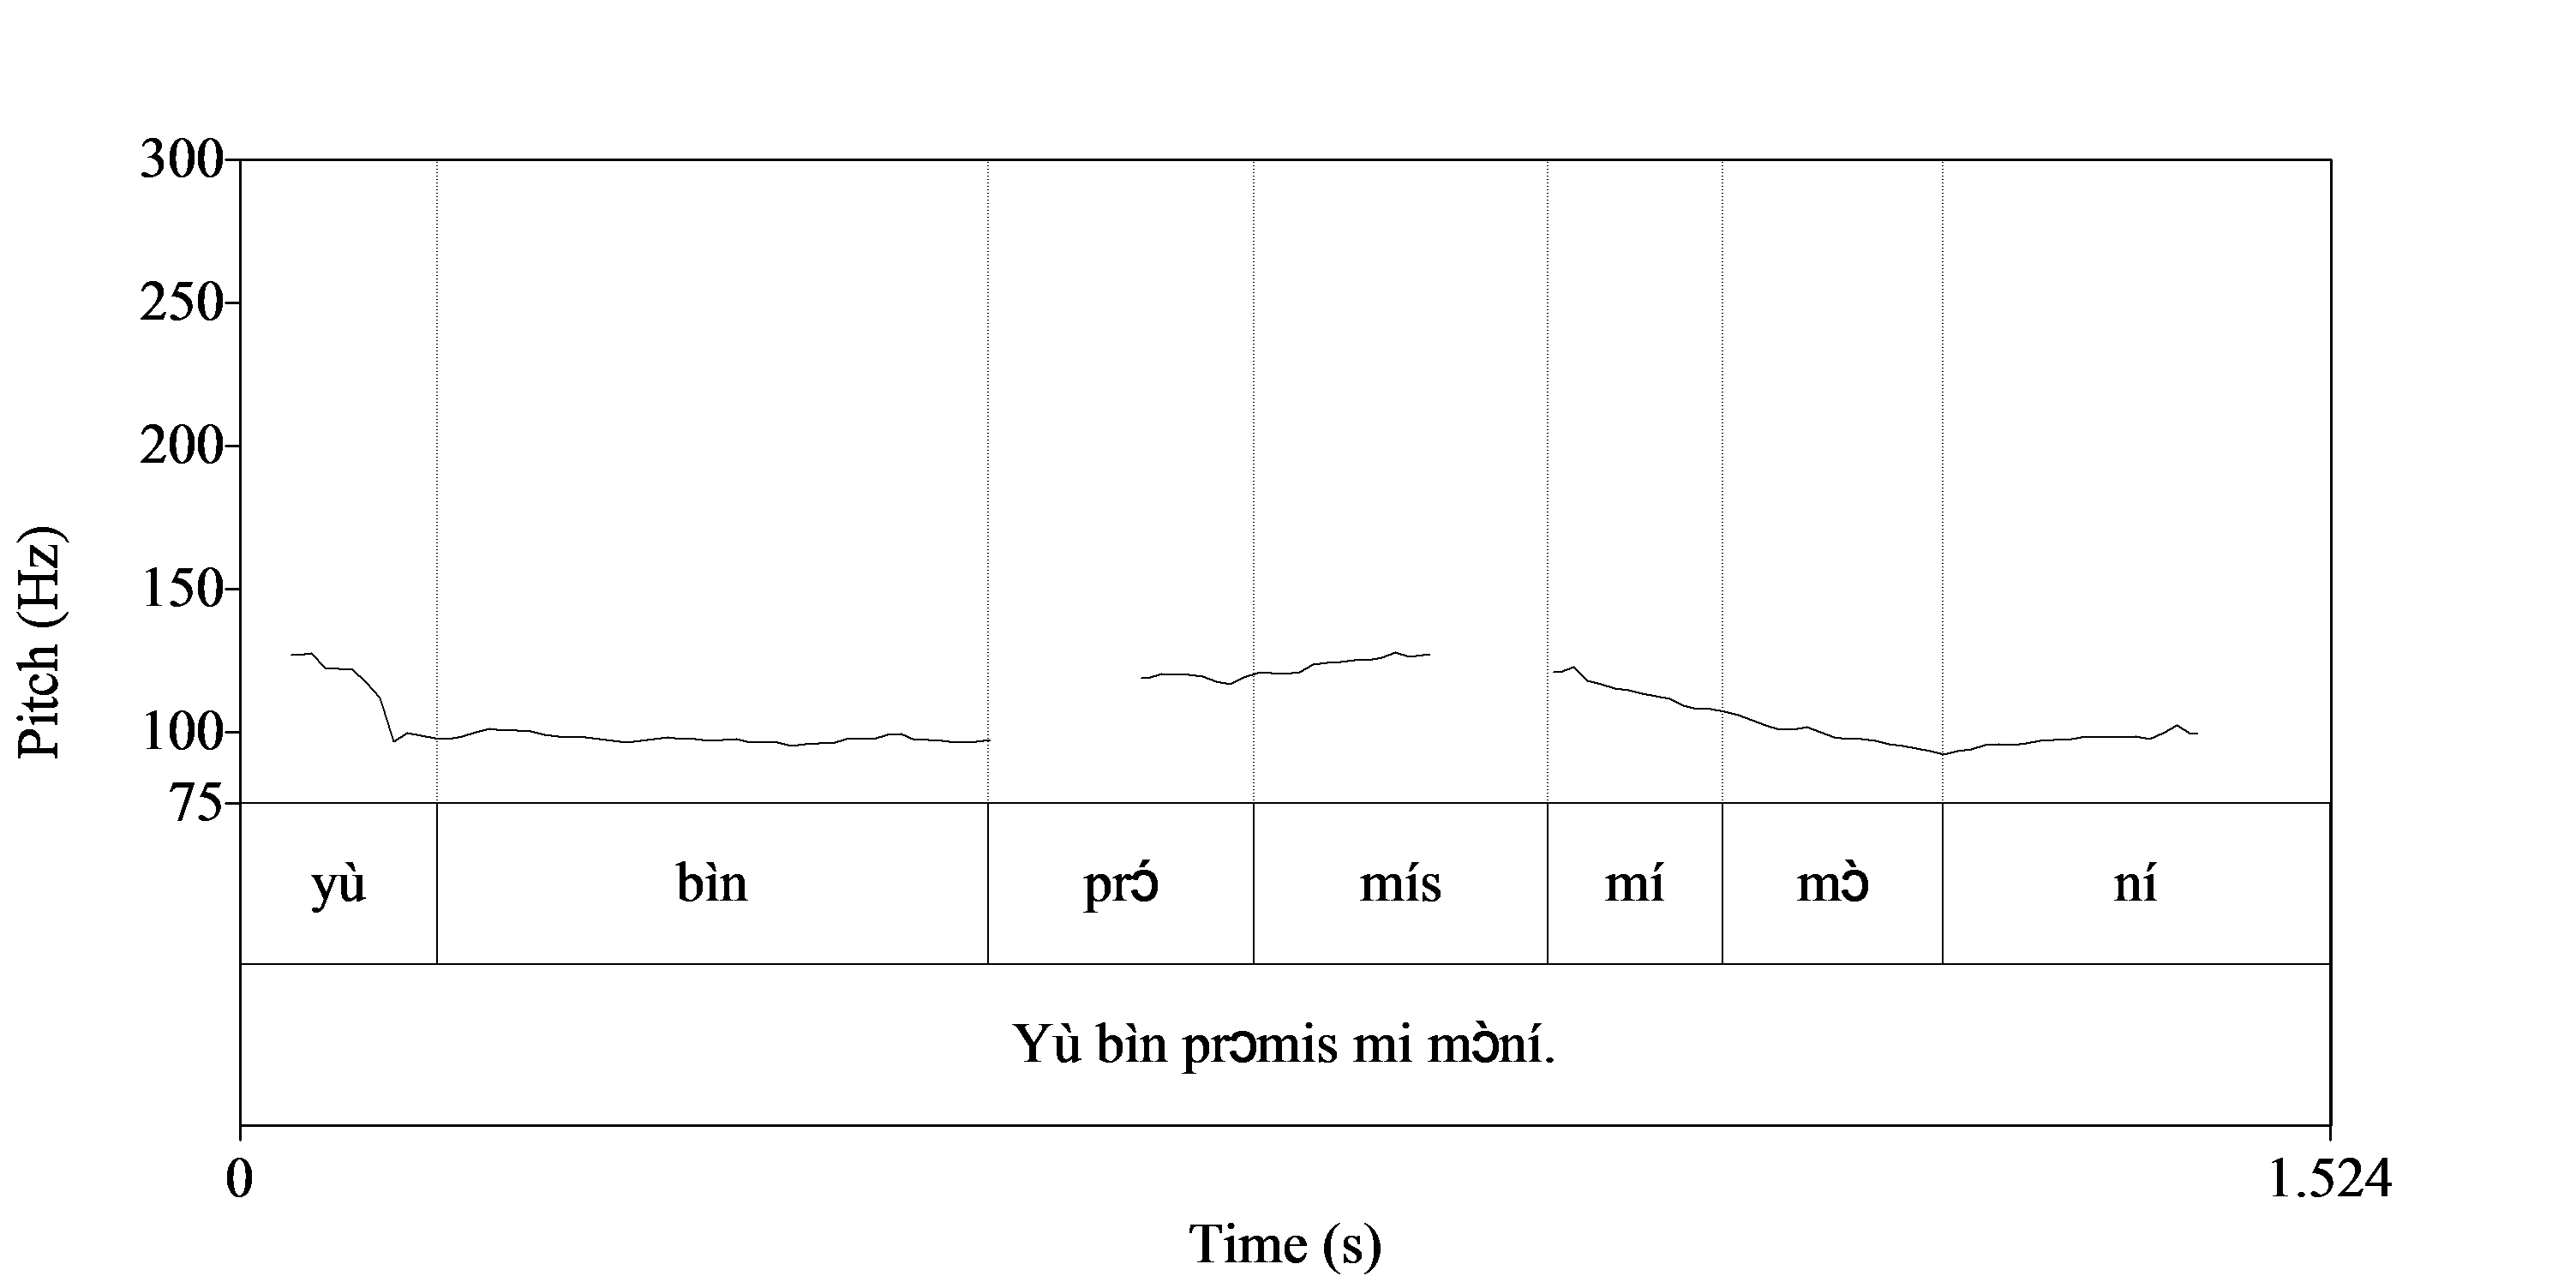
\includegraphics[height=.3\textheight]{figures/yakpomod-img13.png}
\label{fig:key:3.11}
\end{figure}
 


\ea%50
    \label{ex:key:50}
    \glll   Yu  bin  prɔ́mis  mí    mɔní.  →    Yu  bin  \textbf{prɔ́mis}  mí  mɔní.\\
\textsc{l}  \textsc{l}  \textsc{h.l}    \textsc{h}    \textsc{l.h}         {} \textsc{l}  \textsc{l}  \textbf{\textsc{h.h}}    \textsc{h}  \textsc{l.h}\\
\textsc{2sg}  \textsc{pst}  promise  \textsc{1sg.indp}  money\\
\glt ‘You promised me money.’
\z

An environment that is particularly conducive to rightward tone spreading is when the L-toned syllable of a bisyllabic word with an H.L. pattern is hemmed in by the preceding H tone and the H tone of a following object. In \figref{fig:key:3.12}, the L-toned syllable of \textit{fínis} ‘finish’ is raised in pitch approximately to the level of the following object \textit{skúl} ‘school’. The pitch trace in \figref{fig:key:3.13} exemplifies the same process with \textit{vɔ́mit} ‘vomit’ and the following object \textit{chɔ́p} ‘food’:

% TODO: put in a cuadrant

\begin{figure}
\caption{H tone spreading}
\label{fig:key:3.12}
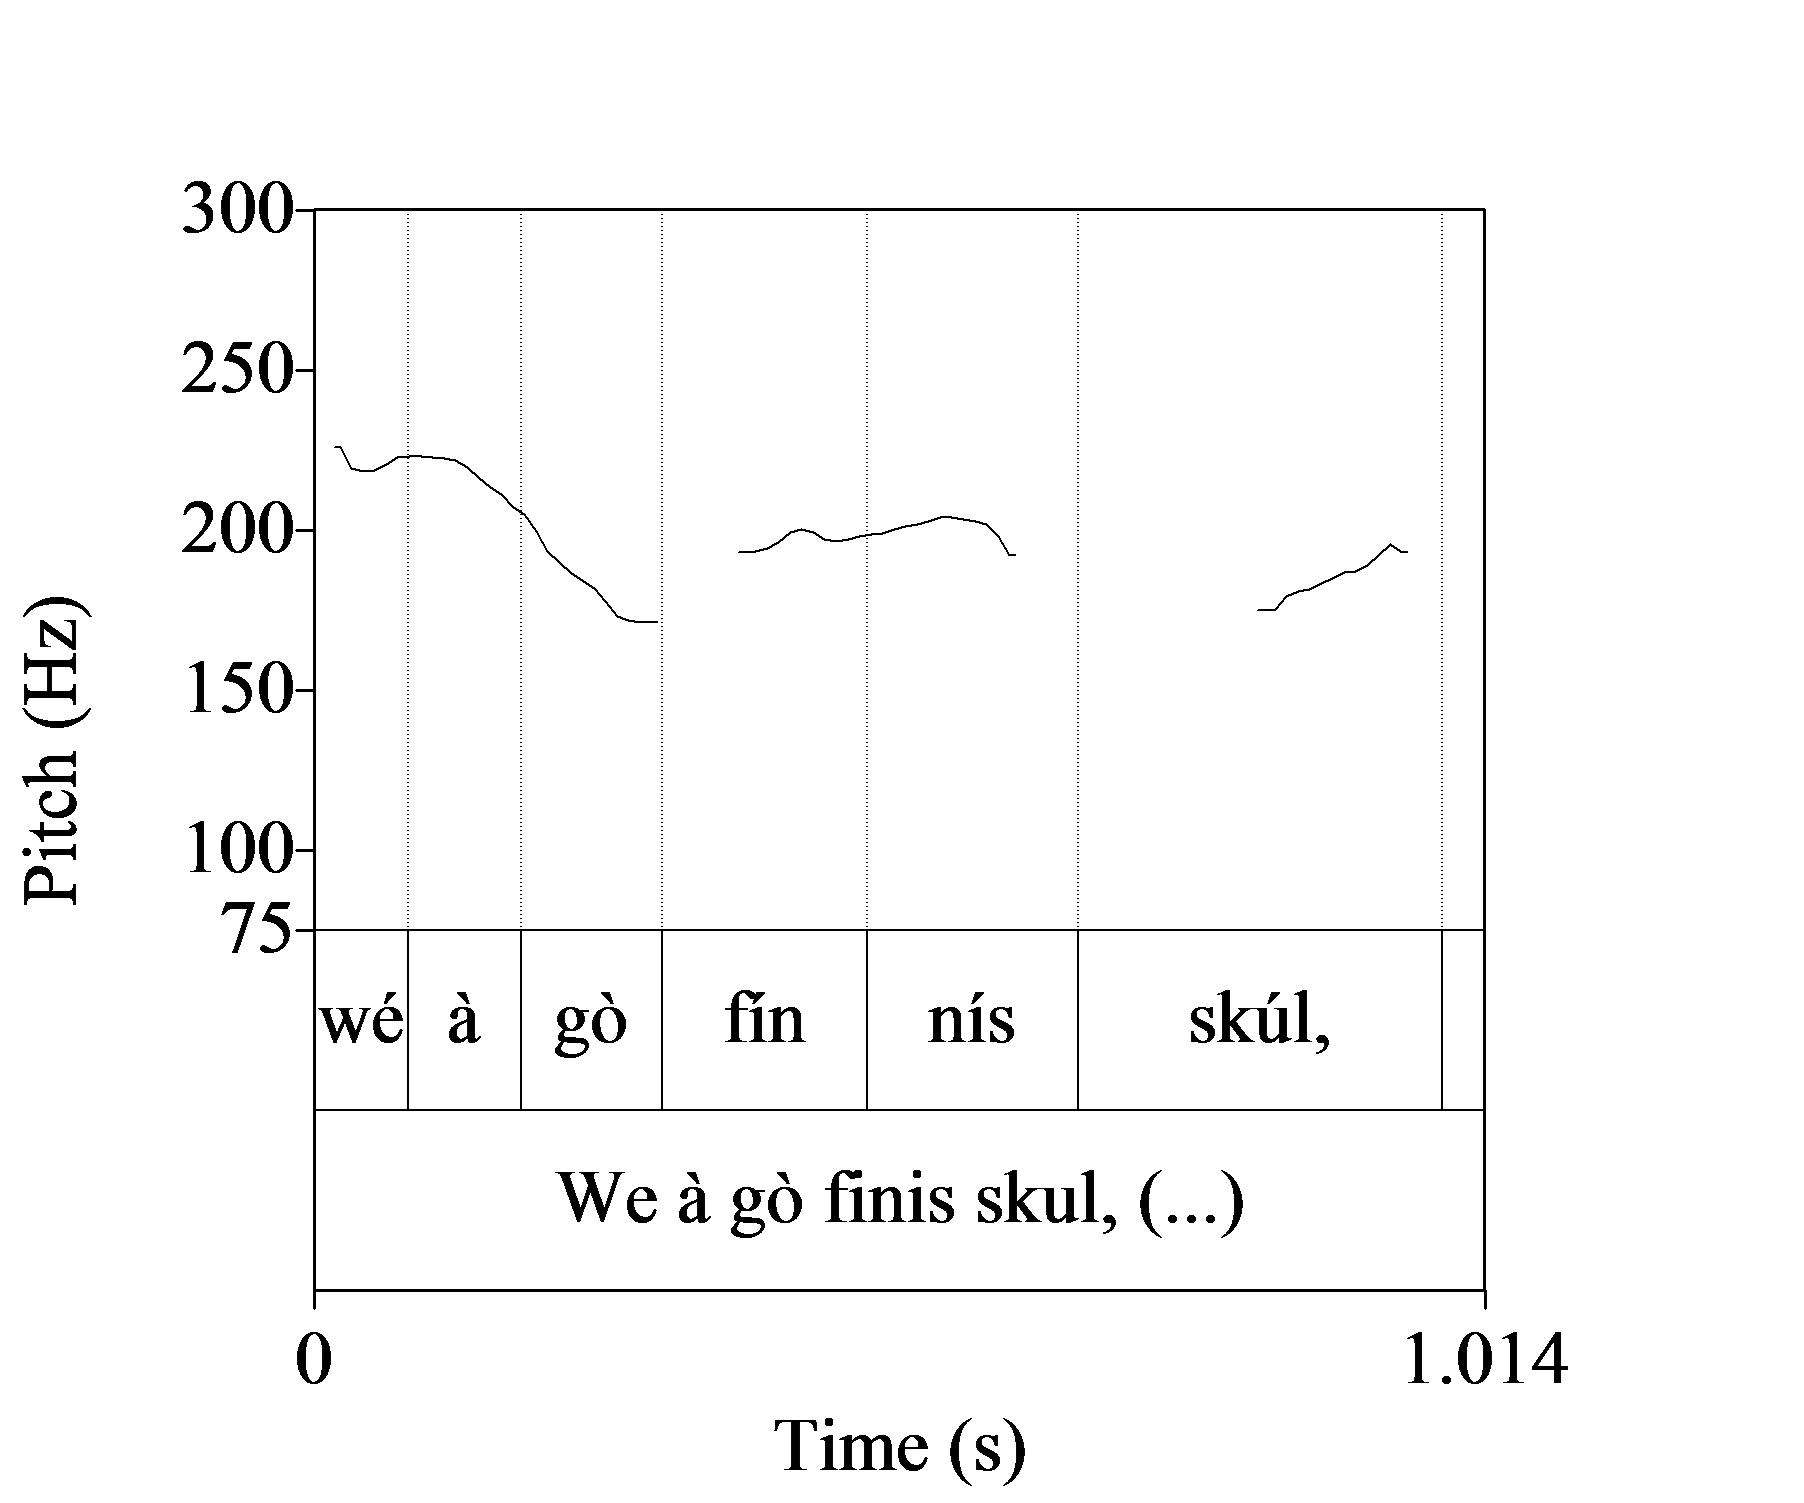
\includegraphics[height=.3\textheight]{figures/yakpomod-img14.png}
\end{figure}

\begin{figure}
\caption{H tone spreading}
\label{fig:key:3.13}
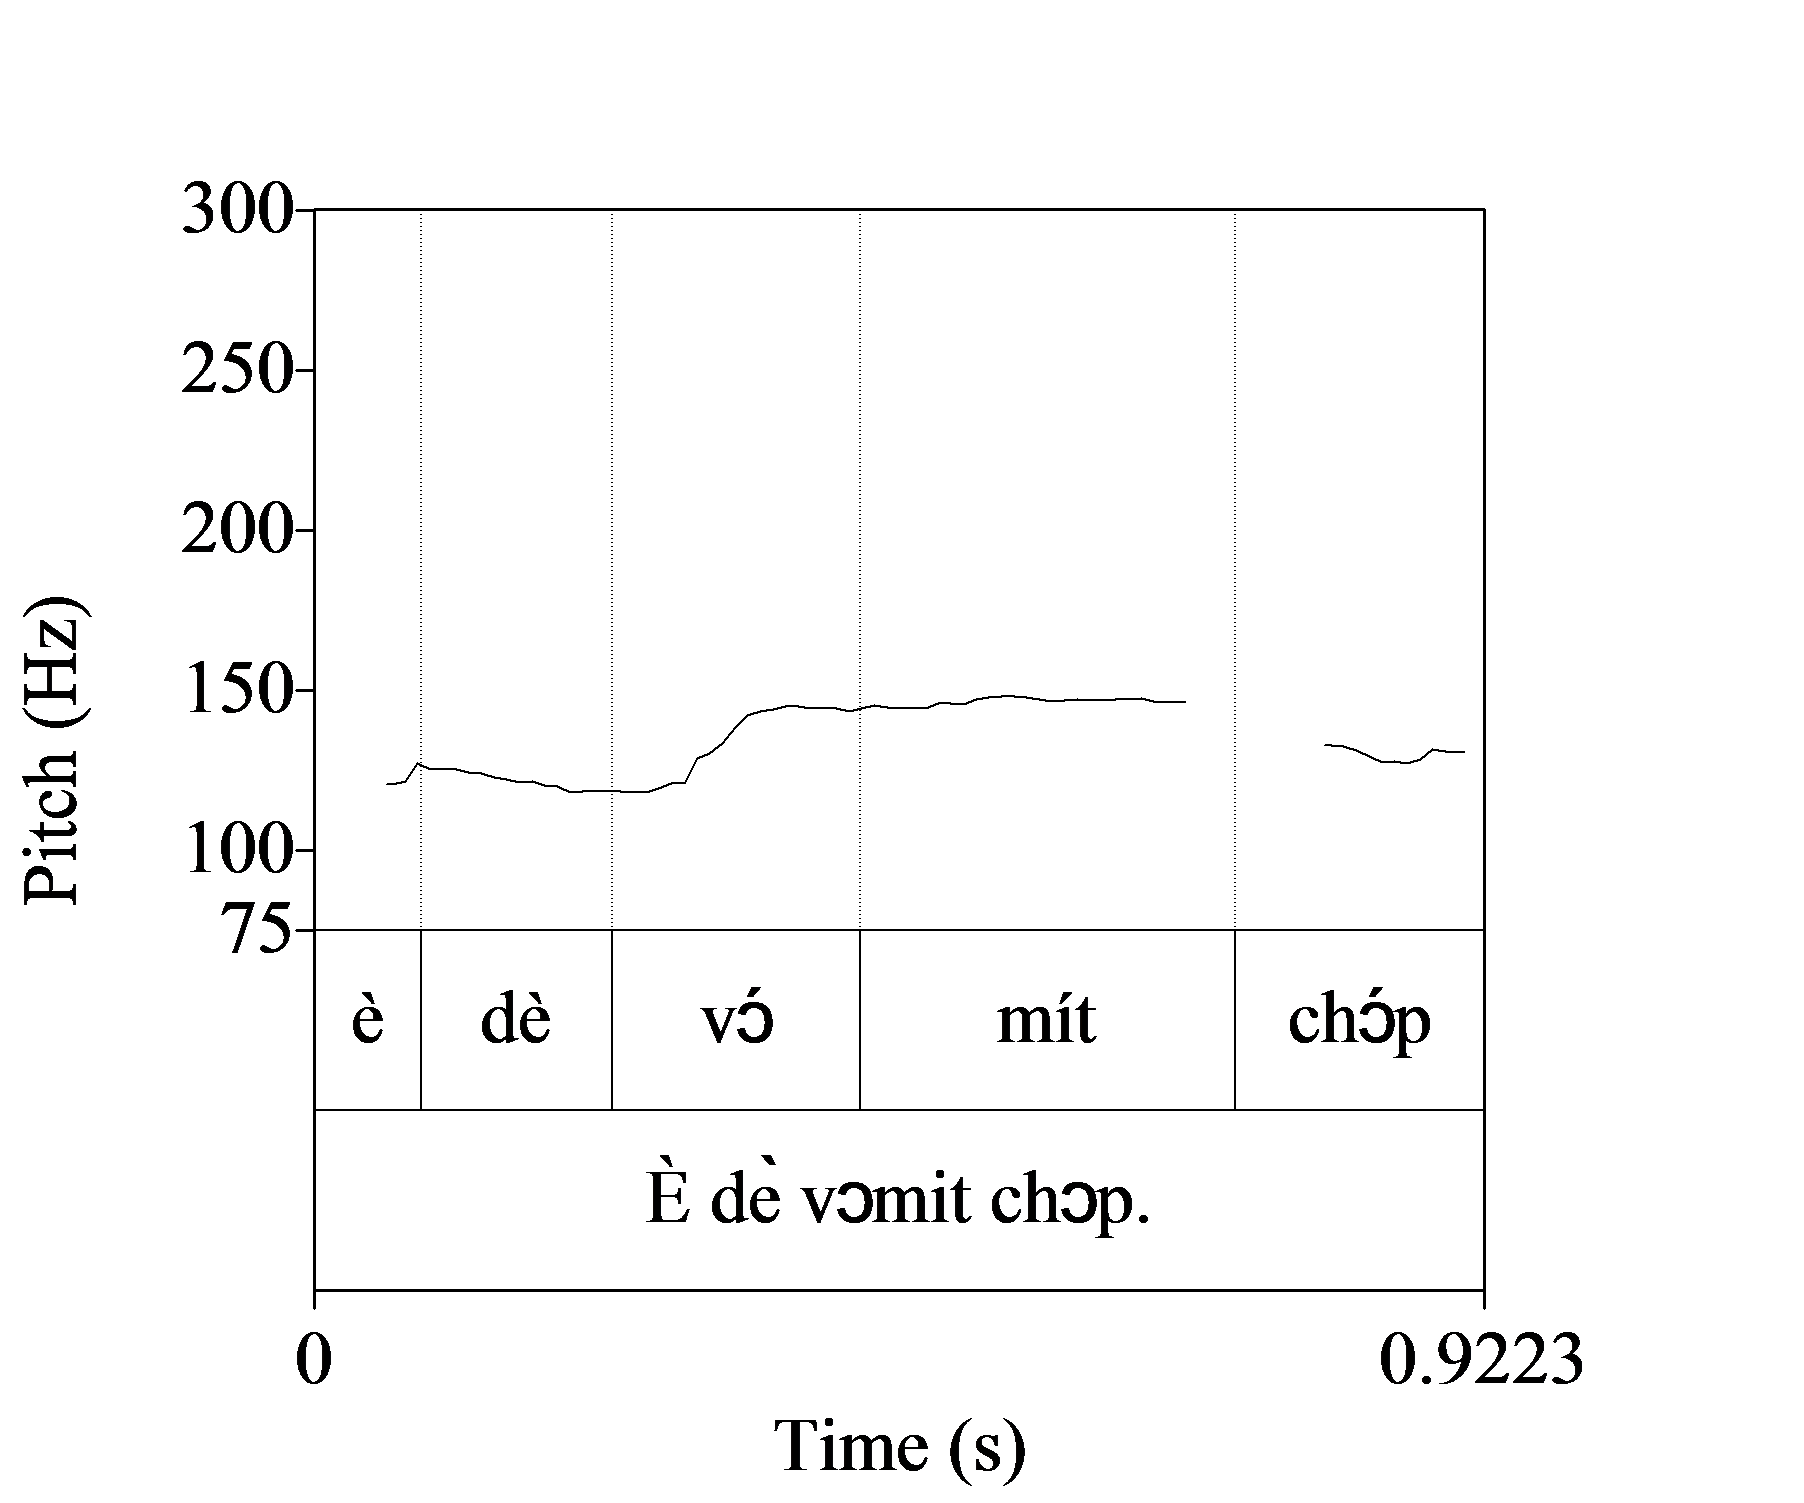
\includegraphics[height=.3\textheight]{figures/yakpomod-img15.png} 
\end{figure}

\ea\label{ex:key:51}
\glll Wé  a    go  fínis    skúl  (...)\\
\textsc{h}  \textsc{l}    \textsc{l}  \textsc{h.l}    \textsc{h}\\
\textsc{sub}  \textsc{1sg.sbj}  \textsc{pot}  finish  school\\
\glt  ‘When I finish school.’  →\\
\gll    Wé  a  go  \textstylePichiexamplebold{finís}  \textstylePichiexamplebold{skúl}  (...)\\
\textsc{h}  \textsc{l}  \textsc{l}  \textbf{\textsc{h.h}}    \textbf{\textsc{h}}\\
\z
\ea\label{ex:key:52}   
\glll E    de    vɔ́mit  chɔ́p.\\
\textsc{l}    \textsc{l}    \textsc{h.l}    \textsc{h}\\
\textsc{3sg.sbj}  \textsc{ipfv}    vomit  food\\
\glt  ‘He is vomiting (the) food.’  →\\
\gll E  de  \textstylePichiexamplebold{vɔmít}  \textstylePichiexamplebold{chɔ́p}.\\
\textsc{l}  \textsc{l}  \textbf{\textsc{h.h}  }  \textbf{\textsc{h}}\is{assimilation of segments“ r}\\
\z
A second phono-syntactic environment that favours rightward H tone spreading is a modifier-noun phrase. The L-toned syllable of a bisyllabic property item in prenominal position and with an H.L pattern may be raised to H if it is immediately followed by a noun with an initial (or only) H tone. An example for this process is provided in \REF{ex:key:58} further below. In the NP, the L-toned syllable of the modifier \textit{fúlis} ‘foolish’ is raised to an H tone because it is followed by the H-toned noun \textit{mán} ‘man’.

\subsection{Floating}\label{sec:3.2.2}

Pichi makes extensive use of floating boundary tones for the purpose of intonation. Aside from that, a lexical tone may be set afloat when two adjoining vowels merge or one of two adjoining vowels is deleted. Tone floating is particularly likely to occur in the contact zone between an H-toned high-frequency function word and a following L-toned vowel. In \figref{fig:key:3.14}, the final consonant /k/ of \textit{mék} ‘\textsc{sbjv}’ is deleted\index{}. This creates a vowel hiatus, which in turn leads to the deletion of the first, higher /e/ of \textit{mék} in favour of the second, lower vowel /à/. The rising–falling contour over \textit{mâ (mék=à)} is clearly visible. 


In \figref{fig:key:3.15}, the final segment of \textit{háw} ‘how’ is deleted and the lexical H tone is set afloat. The vowel merger between /a/ and the following low-toned dependent personal pronoun \textit{e} creates an HL contour tone: 

% TODO: put in quadrant

\begin{figure}
\caption{Vowel deletion sets tone afloat}
\label{fig:key:3.14}
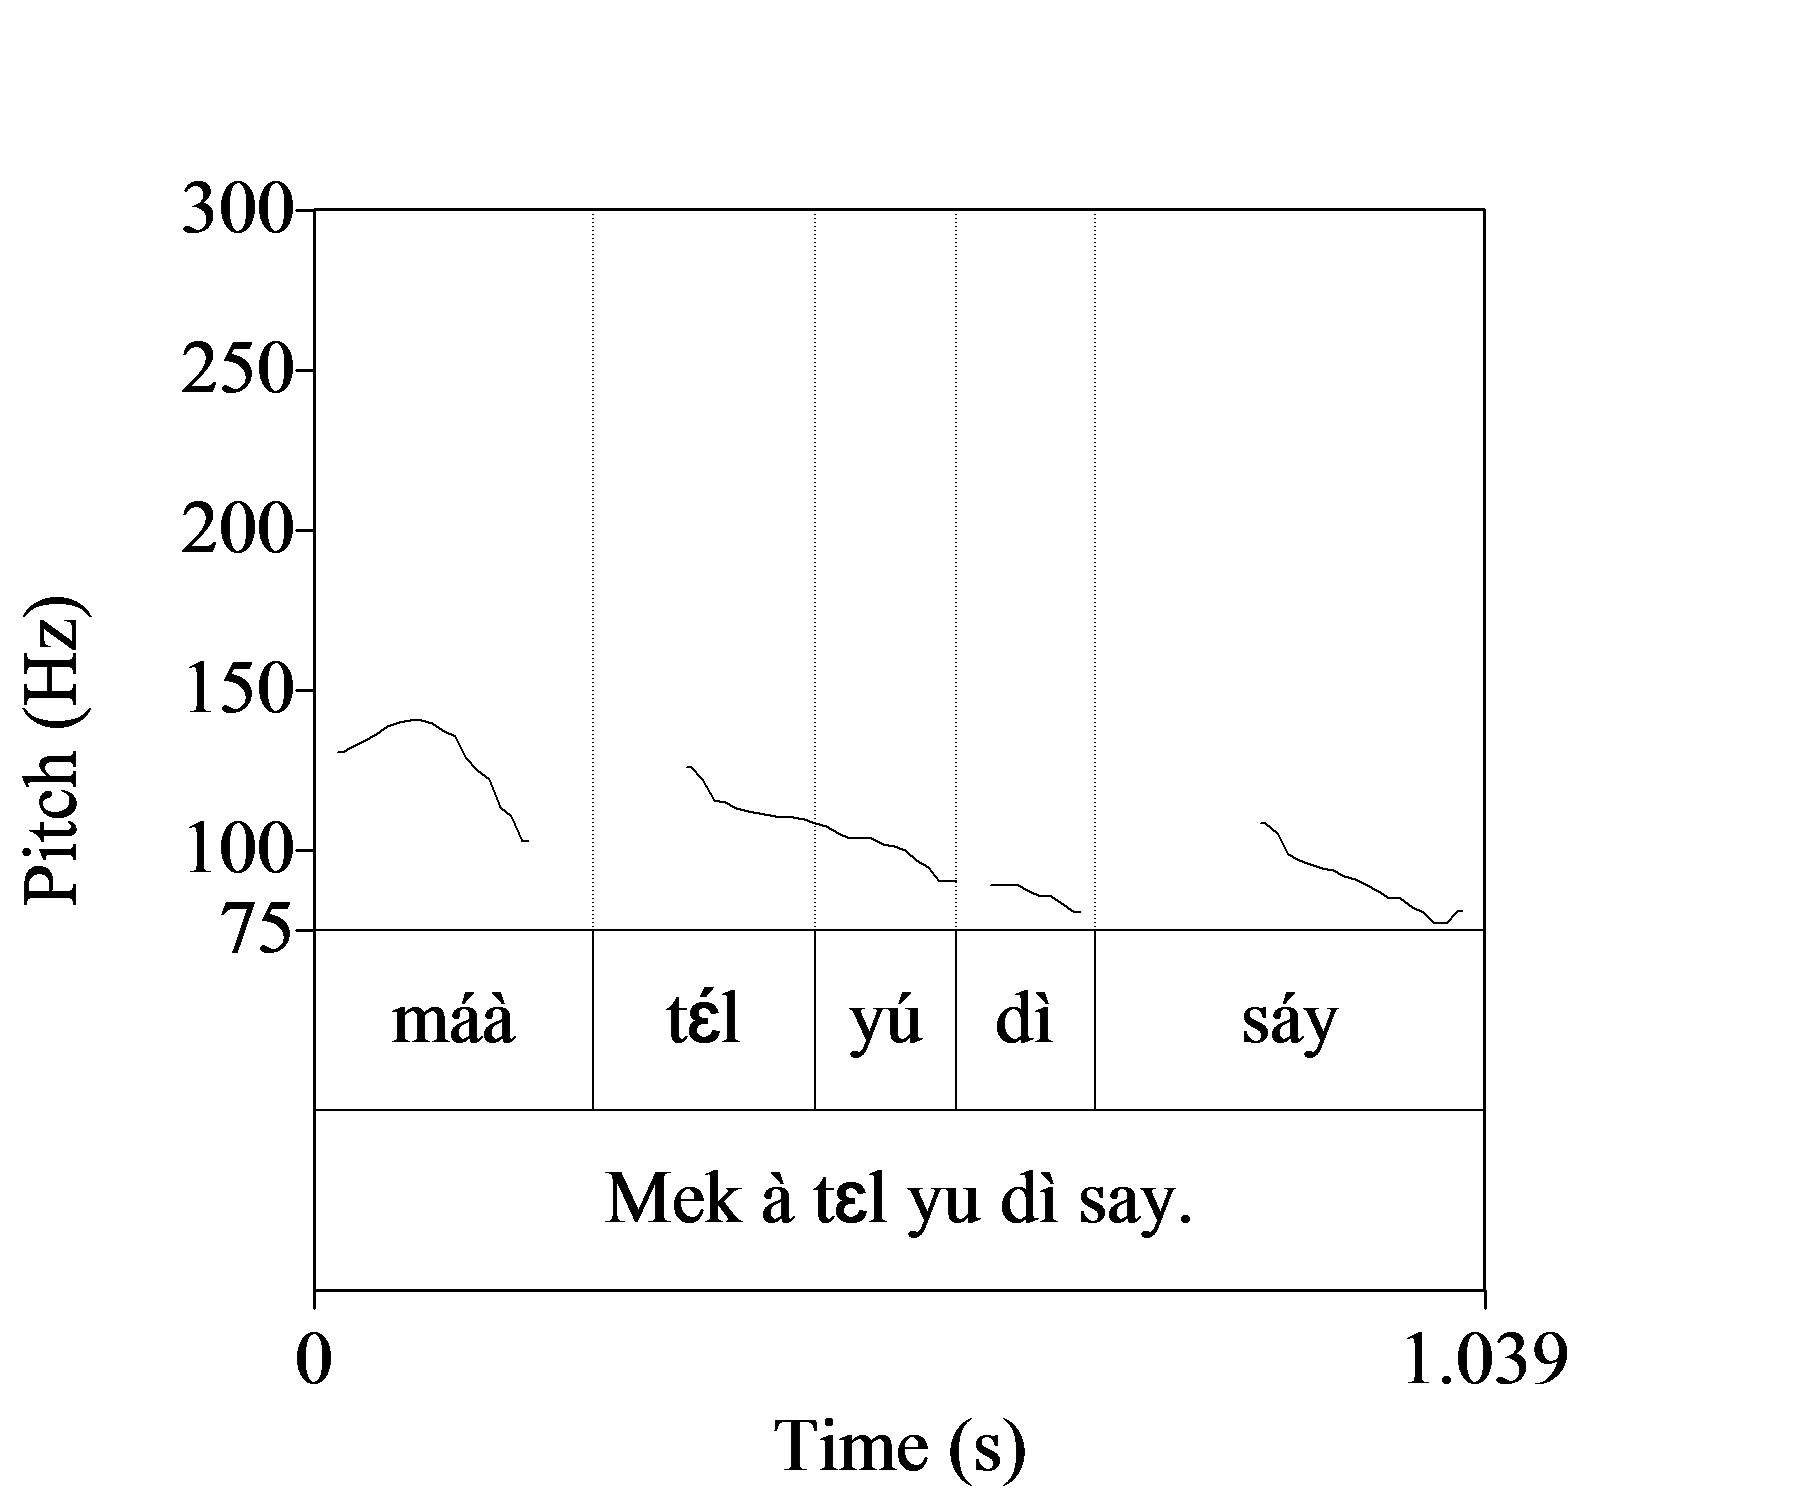
\includegraphics[height=.3\textheight]{figures/yakpomod-img16.png}
\end{figure}

\begin{figure}    
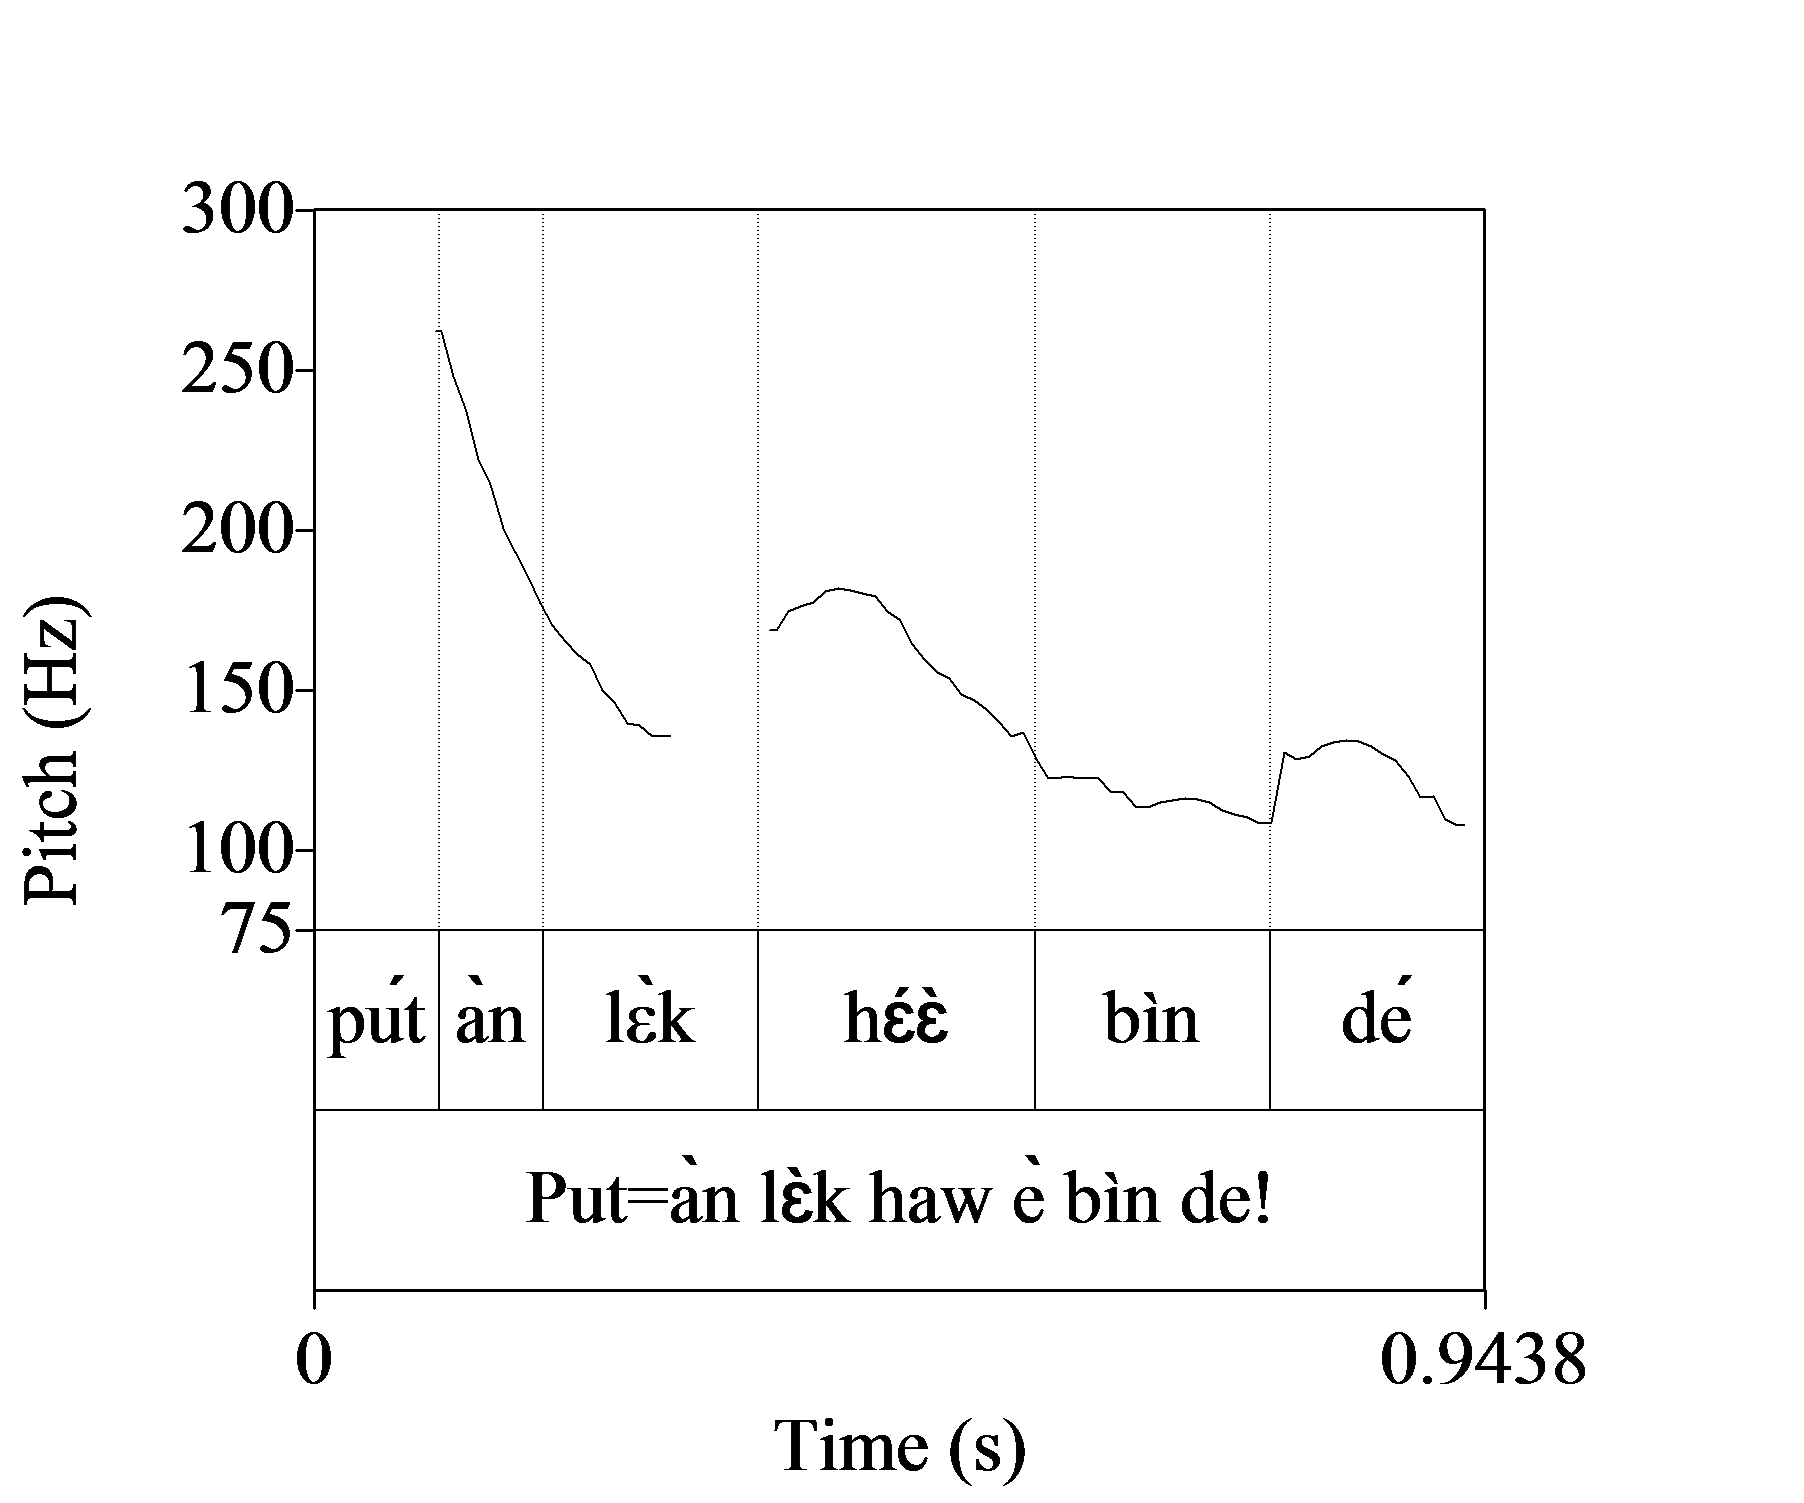
\includegraphics[height=.3\textheight]{figures/yakpomod-img17.png}
\caption{Vowel merger sets tone afloat}
\label{fig:key:3.15} 
\end{figure}

\ea\label{ex:key:53}
\glll Mék    a    tɛ́l  yú    di  sáy.\\
\textsc{h}    \textsc{l}    \textsc{h}  \textsc{h}    \textsc{l}  \textsc{h}\\
\textsc{sbjv}    \textsc{1sg.sbj}  tell  \textsc{2sg.indp}  \textsc{def}  side\\
\glt ‘Let me tell you the place.’    →\\
\gll Mâ    tɛ́l  yú  di  sáy.\\
\textbf{\textsc{hl}}    \textsc{h}  \textsc{h}  \textsc{l}  \textsc{h}\\
\z

\ea\label{ex:key:54}
\glll   Pút=an    lɛk  háw  e    bin  dé!\\
\textsc{h}  \textsc{l}    \textsc{l}  \textsc{h}  \textsc{l}    \textsc{l}  \textsc{h}\\
put=\textsc{3sg.obj}  like  how  \textsc{3sg.sbj}  \textsc{pst}  \textsc{be.loc}\\
\glt ‘Put it like it was!’    →\\
\gll Pút=an  lɛk  \textbf{hɛ}  bin  dé!\\
\textsc{h}  \textsc{l}  \textsc{l}  \textbf{\textsc{hl}}  \textsc{l}  \textsc{h}\\
\z
\subsection{Downdrift and downstep}\label{sec:3.2.3}

Downdrift and downstep contribute to a general downward cline of pitch in utterances. An utterance normally begins with a high pitch onset and declines progressively with every lexical tone. Downdrift (indicated by ↓H) causes an H to be lowered by a preceding L tone as in \figref{fig:key:3.16}. The overall effect of downdrift is visible by the roughly equivalent pitch over the initial L-toned personal pronoun \textit{a} ‘\textsc{1sg.sbj}’ and the final H-toned noun \textit{hós} ‘house’:

\begin{figure}
\caption{Downdrift}
\label{fig:key:3.16}
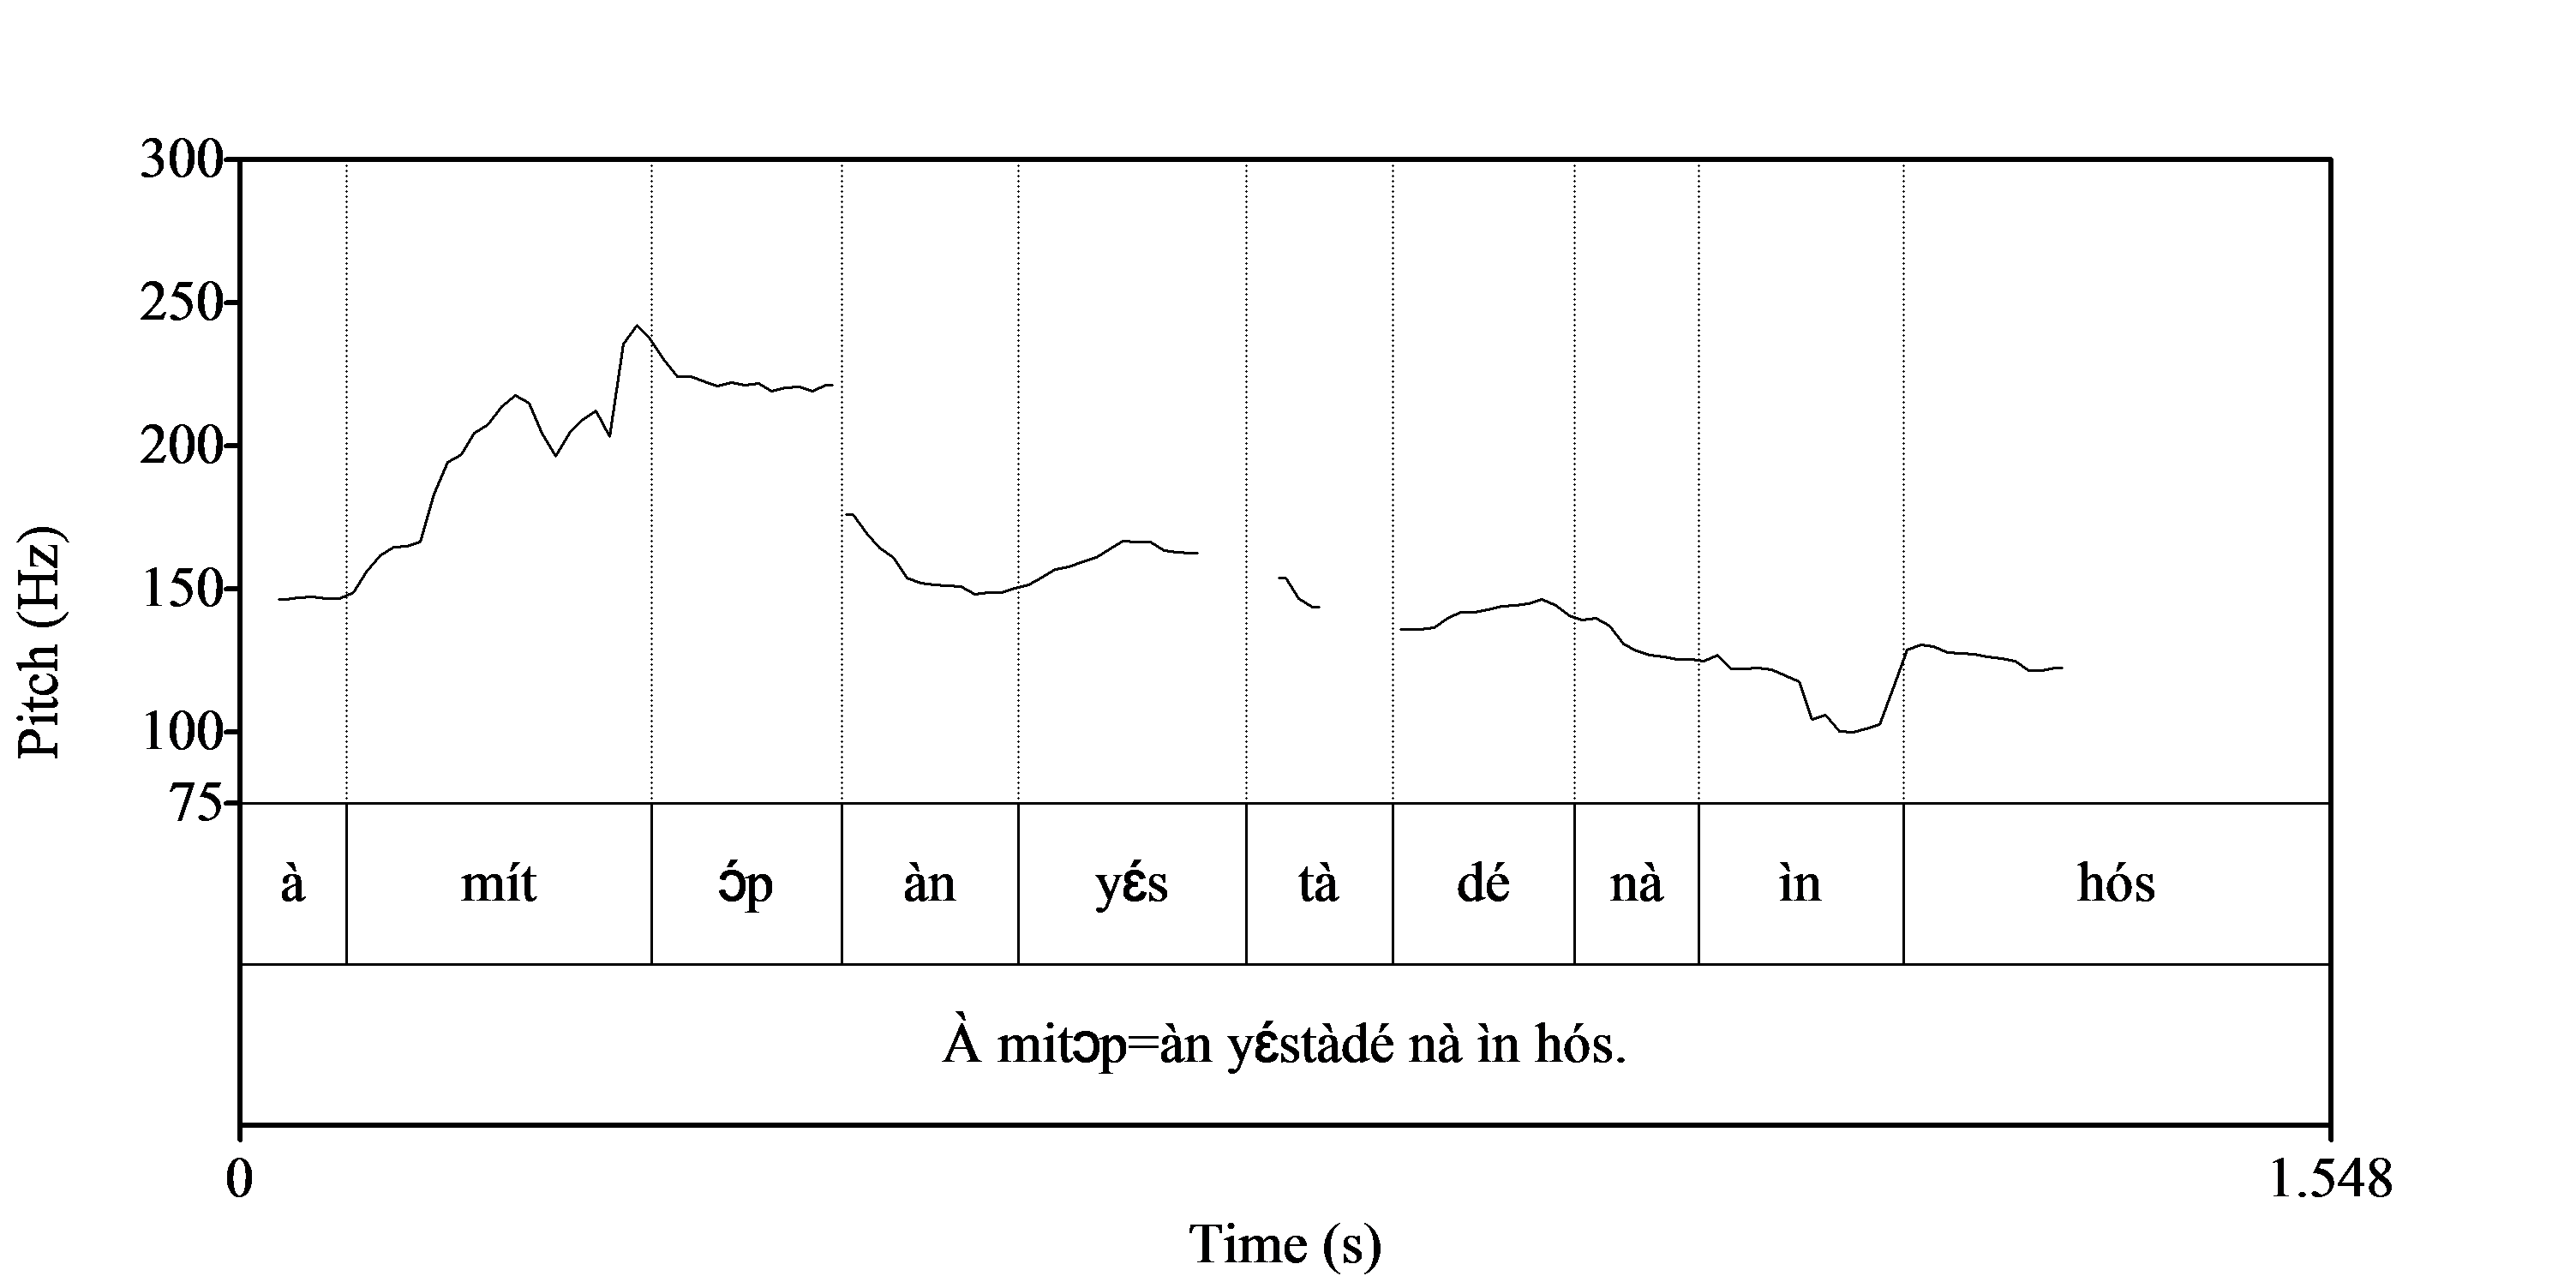
\includegraphics[height=.3\textheight]{figures/yakpomod-img18.png}
\end{figure}
 


\ea%55
    \label{ex:key:55}
    \glll   A    mítɔp=an  yɛ́stadé    na  in  hós.\\
\textsc{l}    \textstylePichiexamplebold{\textmd{\textsc{h}}}\textsc{.h=l}    \textsc{↓}\textbf{\textsc{h}}\textsc{.l.↓}\textbf{\textsc{h}}    \textsc{l}  \textsc{l}  \textsc{↓}\textbf{\textsc{h}}\is{downdrift} \\
\textsc{1sg.sbj}  meet=\textsc{3sg}  yesterday  \textsc{loc}  \textsc{3sg.poss}  house\\
\glt ‘I met him yesterday in his house.’    
\z


The second phenomenon involving declination is downstep\is{downstep} (indicated by –H). In a series of adjacent H tones, each tone may be lowered successively in relation to the preceding one. Downstep is exemplified below by the two successive homophones in \figref{fig:key:3.17} and the iteration in \figref{fig:key:3.18} below. We also find downdrift in both examples:

% TODO: put in quadrant
 
\begin{figure}
\caption{Downstep}
\label{fig:key:3.17}
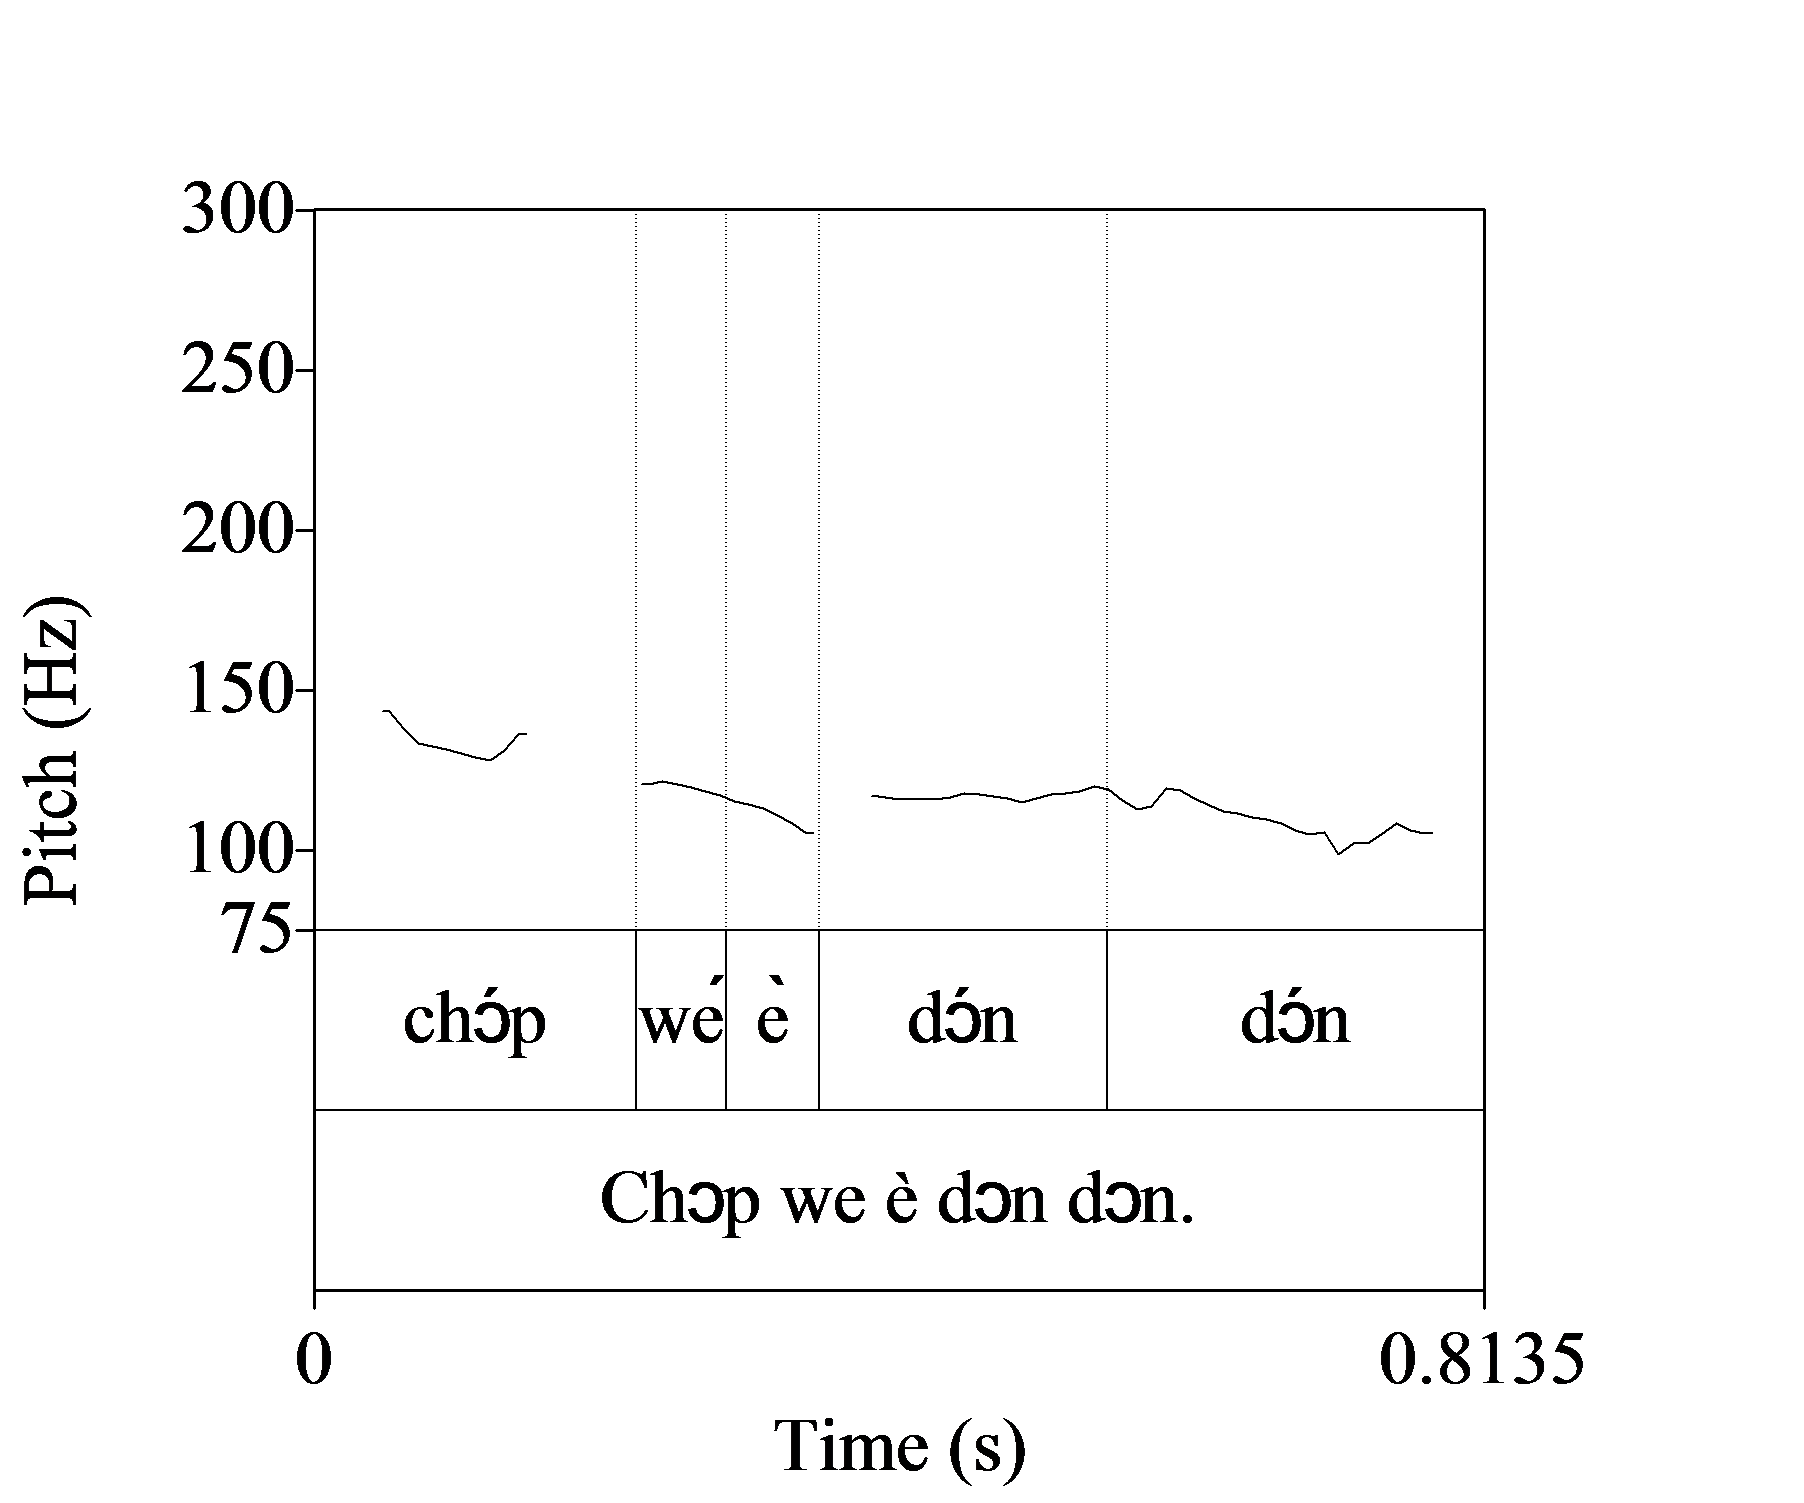
\includegraphics[height=.3\textheight]{figures/yakpomod-img19.png}
\end{figure}

\begin{figure}    
\caption{Downstep}
\label{fig:key:3.18}
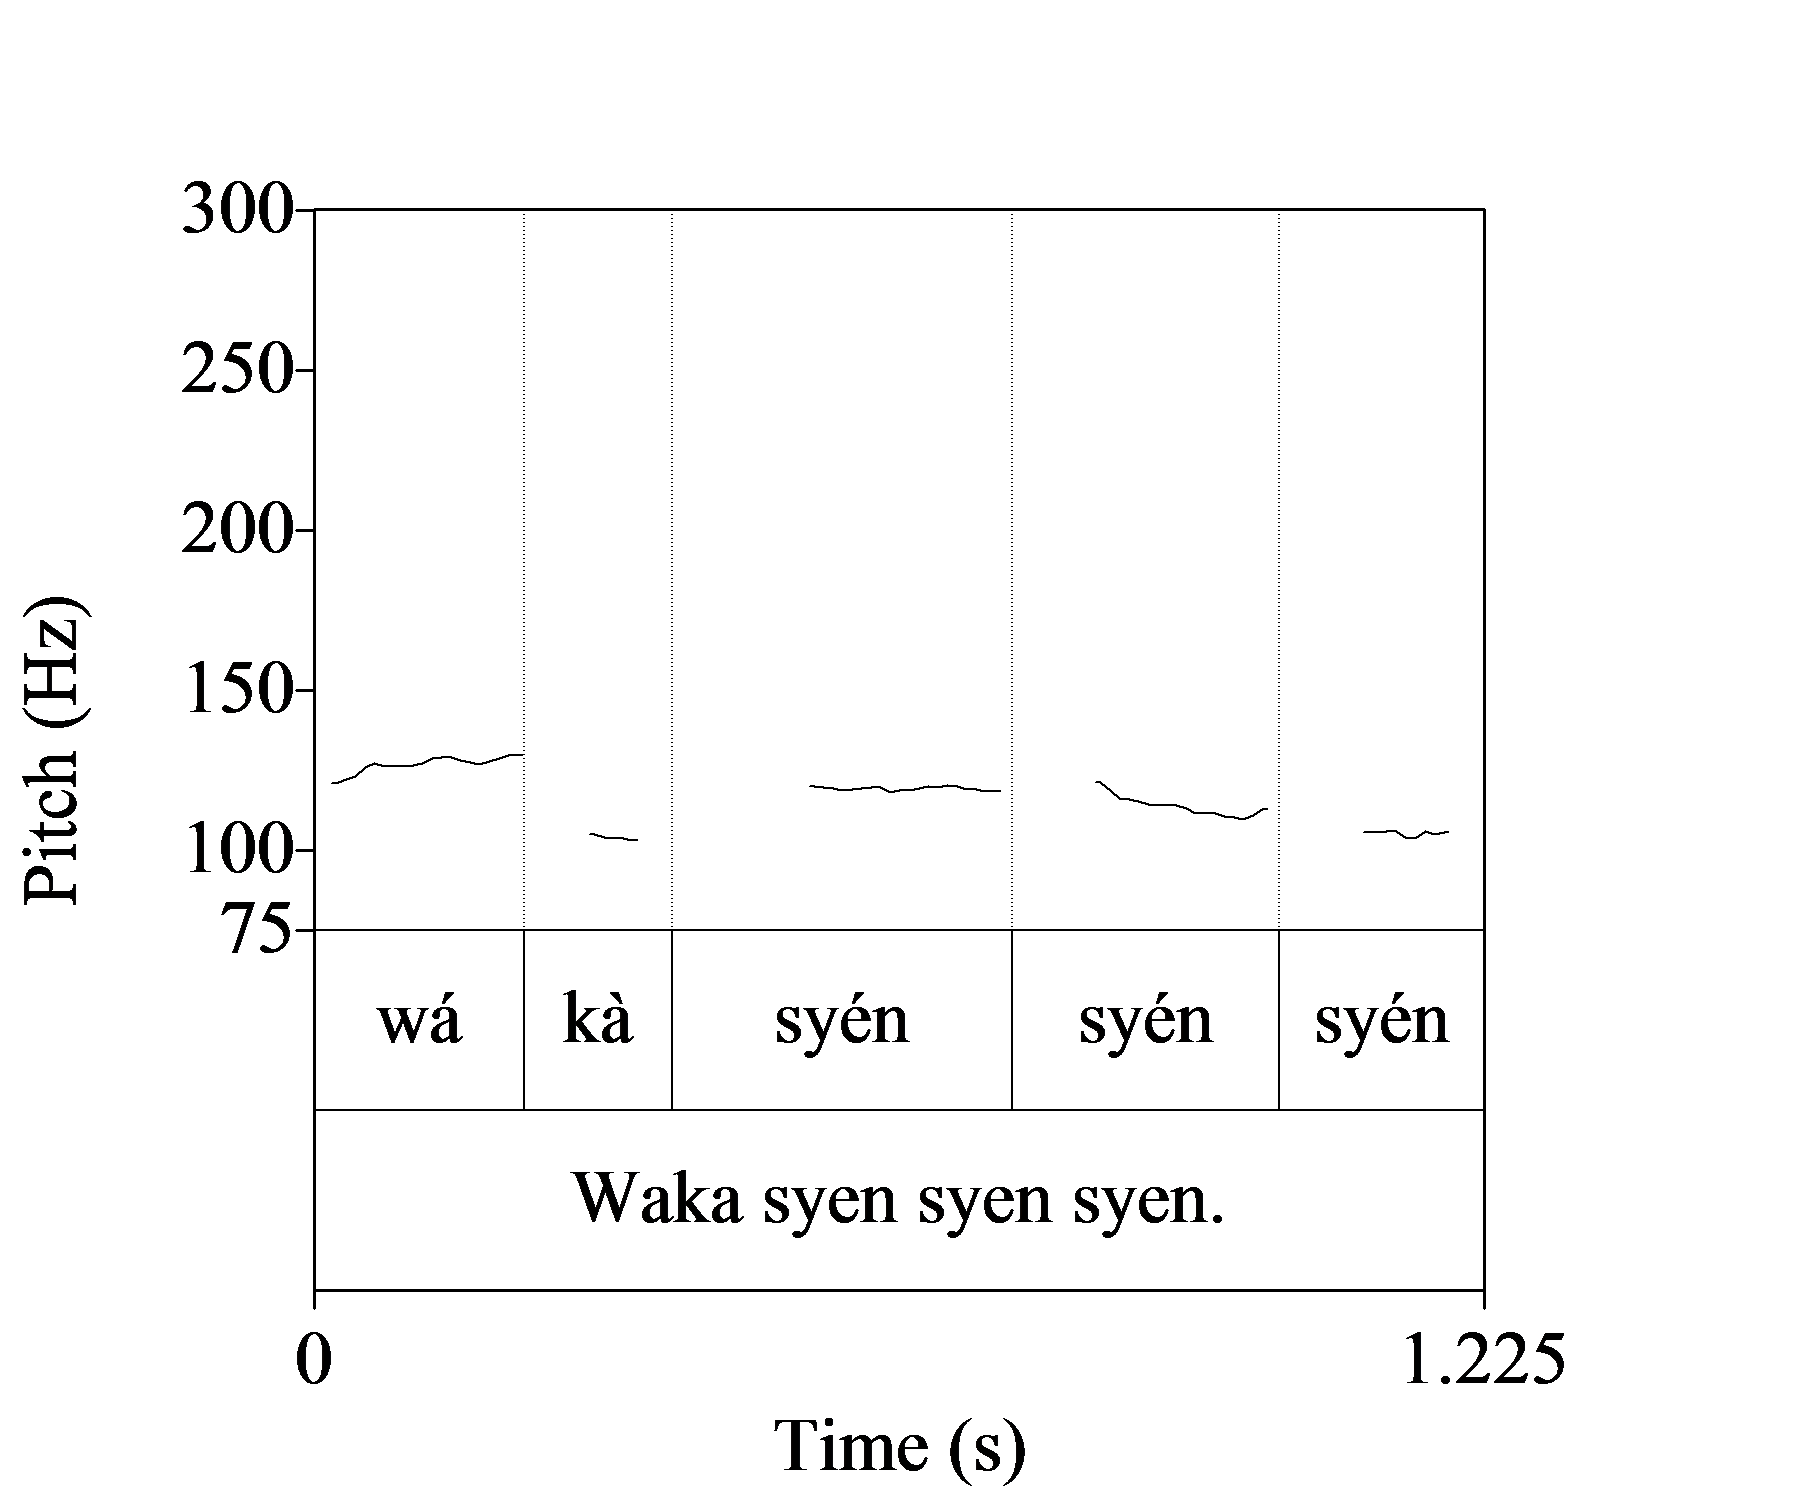
\includegraphics[height=.3\textheight]{figures/yakpomod-img20.png} 
\end{figure}

\ea\label{ex:key:56}
\glll Chɔ́p  wé  e    \textbf{dɔ́n}  \textbf{dɔ́n}.\\
\textsc{h}    \textbf{\textsc{{}-h}}  \textsc{l}    \textsc{↓}\textsc{h}  \textbf{\textsc{{}-h}} \\
food    \textsc{sub}  \textsc{3sg.sbj}  \textsc{prf}  done\\
\glt ‘Food that is done.’
\z

\ea\label{ex:key:57}
\glll   Wáka  sén    \textbf{sén}    \textbf{sén}.\\
\textsc{h.l}    \textsc{↓}\textsc{h}    \textbf{\textsc{{}-h}}    \textbf{\textsc{{}-h}}\\
walk  same  \textsc{rep}    \textsc{rep}\\
\glt ‘Walk exactly in one line.’
\z
\subsection{Deletion}\label{sec:3.2.4}

Tone deletion occurs in two contexts. In compounds (including reduplications), the lexical H tone over the first component is deleted (also see \citealt{Yakpo2012}). The syllable whose tone has been deleted becomes L-toned. The second component retains its original tone pattern. Tone deletion therefore forms an intrinsic part of a derivational process in Pichi (cf. \sectref{sec:4.3}). The second context in which tone deletion occurs is when a boundary tone overrides the utterance-final lexical tone of a word (cf. \sectref{sec:3.4.4} ).

\figref{fig:key:3.19} presents the pitch trace of an NP headed by the noun \textit{mán} ‘man’. The noun is modified prenominally by the verb \textit{fúlis} ‘(be) foolish’, which has an H.L tone pattern. The pitch of the utterance-final H tone over \textit{mán} stands at roughly the same level (albeit slightly downstepped and falling due to declarative intonation) as that of the preceding H tones over the first and second syllables of \textit{fúlis}. Note that the second, lexically L-toned syllable of \textit{fúlis} bears a phonetic H tone due to tonal plateauing (cf. \sectref{sec:3.2.1}):

\begin{figure}
\caption{Simplex noun}
\label{fig:key:3.19}
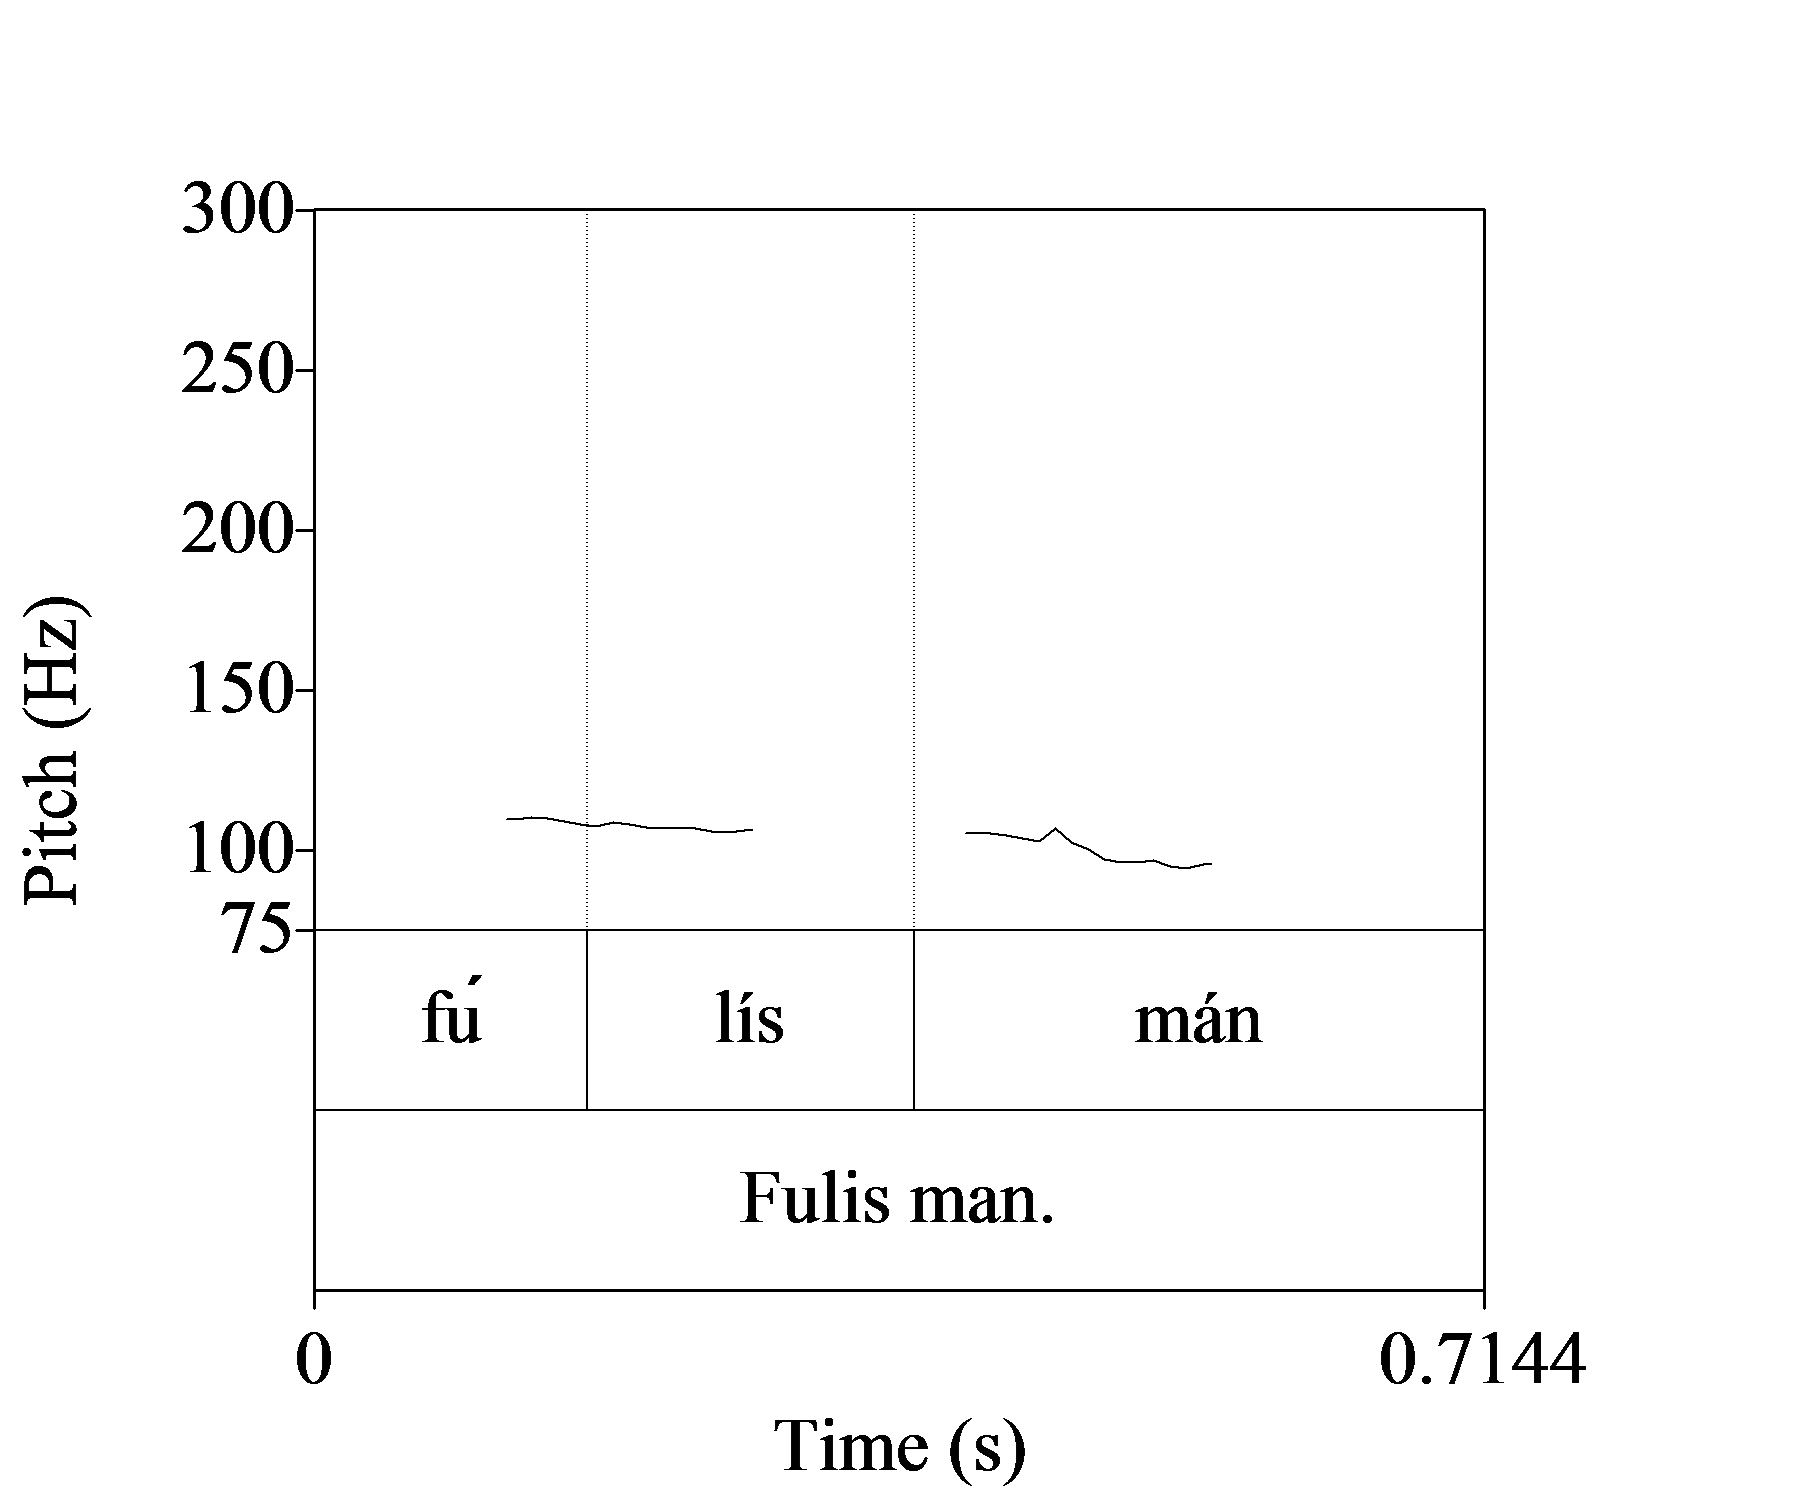
\includegraphics[height=.3\textheight]{figures/yakpomod-img21.png}
\end{figure}

\begin{figure}
\caption{Compound noun}
\label{fig:key:3.20}
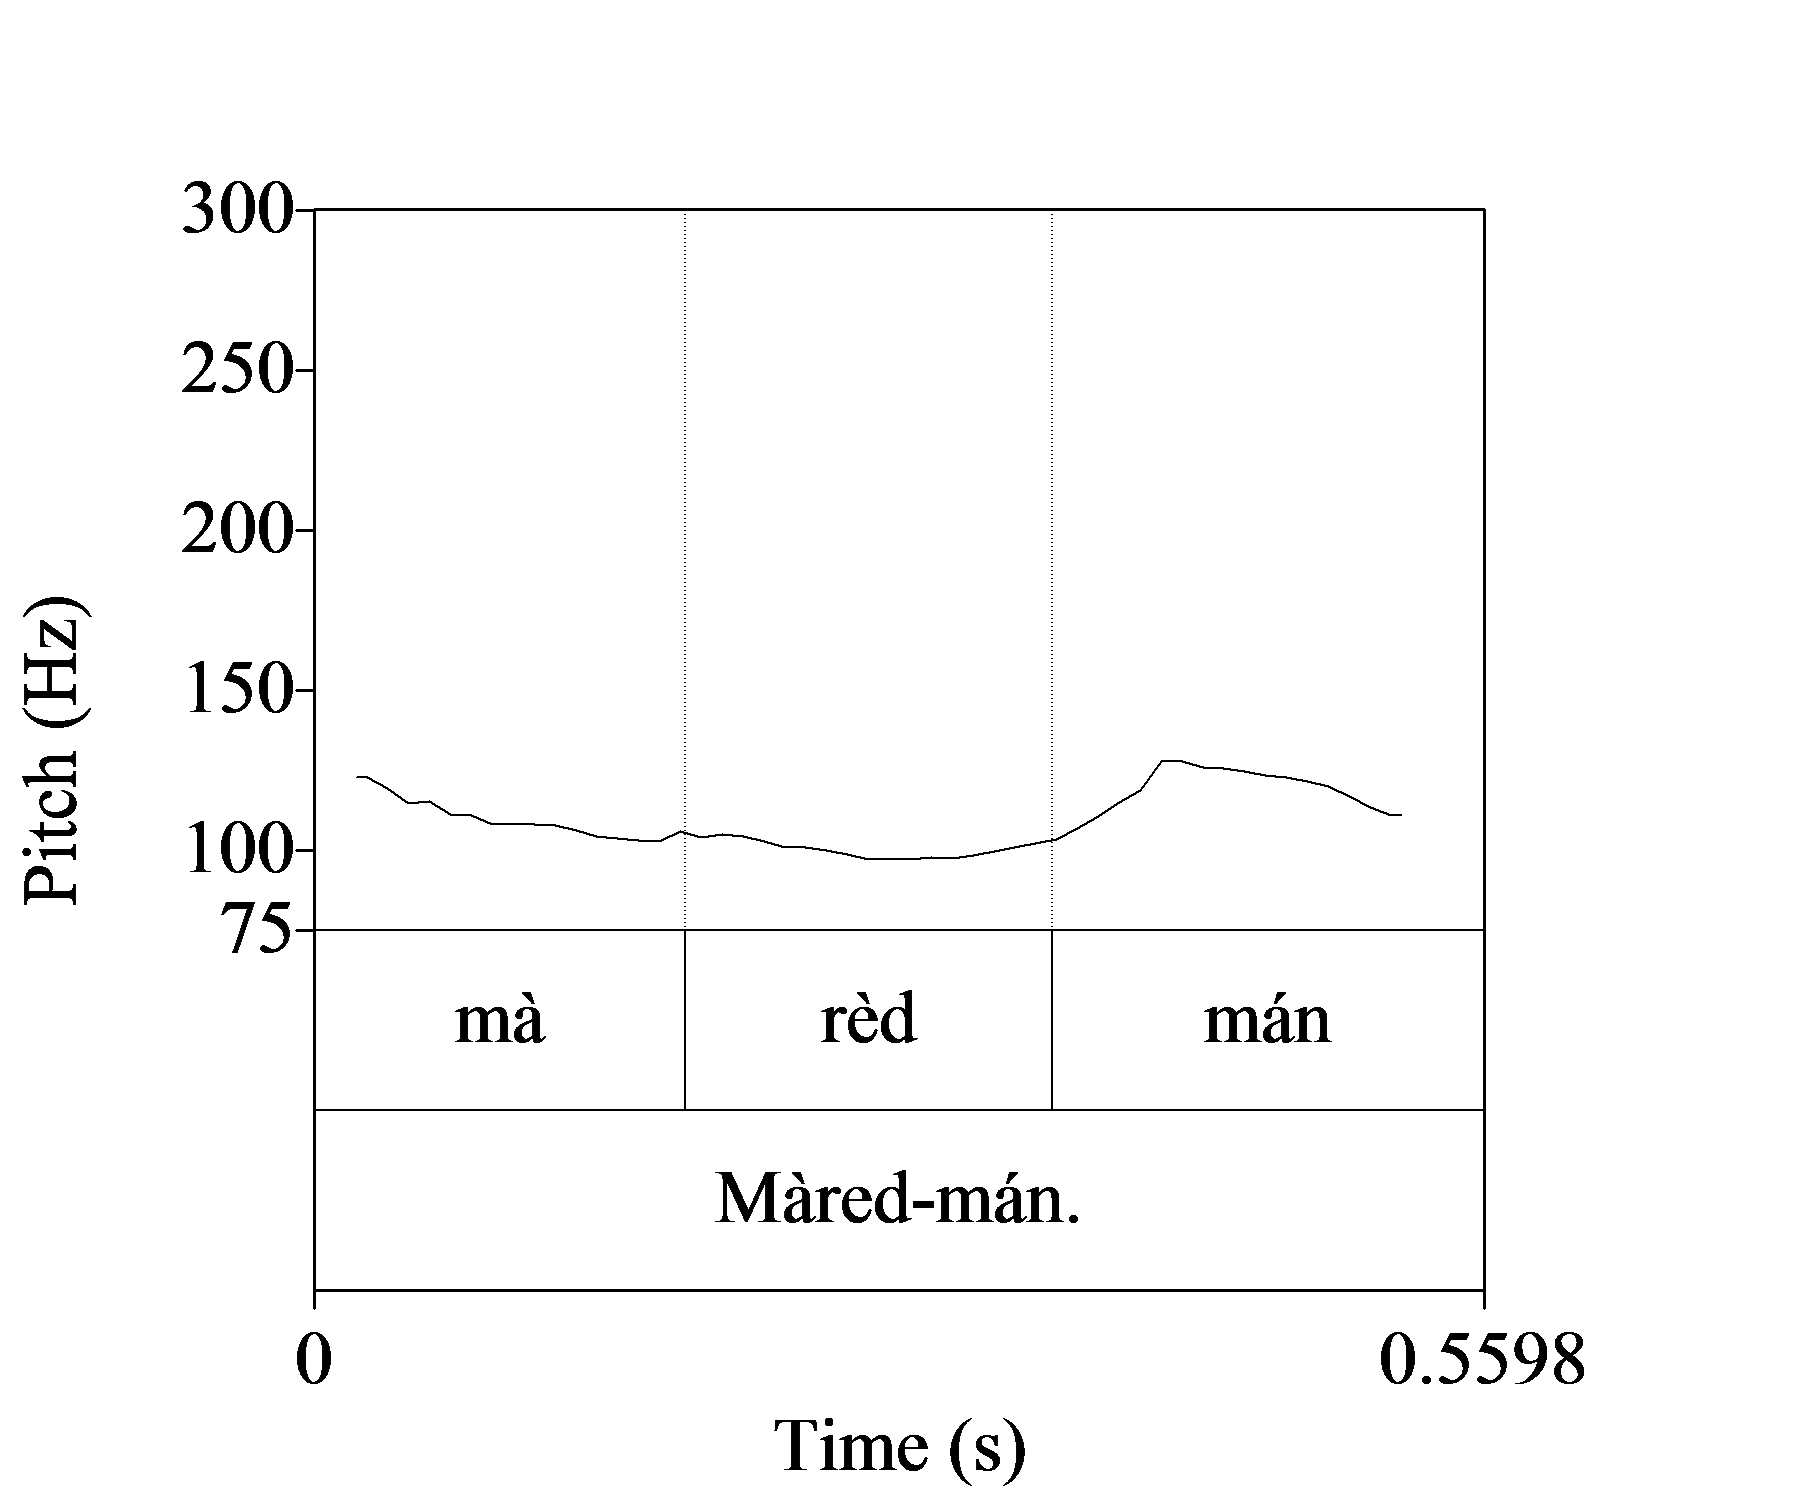
\includegraphics[height=.3\textheight]{figures/yakpomod-img22.png} 
\end{figure}

\ea\label{ex:key:58}
\glll   Fúlis  mán.\\
\textsc{h.h}    \textsc{h}\\
foolish  man\\
\glt   ‘Foolish man.’ 
\z
\ea\label{ex:key:59}
\glll    \textstylePichiexamplebold{Mared}{}-mán\\
\textbf{\textsc{l}}.\textsc{l-h}\\
marry.\textsc{cpd}{}-man.\\
\glt ‘Married man.’
\z
In contrast, the pitch trace in \figref{fig:key:3.20} above exemplifies tone deletion. The head noun \textit{mán} ‘man’ is also modified by a verb with an H.L pattern, namely \textit{máred} ‘marry; be married’. However, \textit{máred} and \textit{mán} form a single phonological word, the compound noun \textit{mared-mán} ‘married man’. The H tone over the first syllable of \textit{máred} has been deleted in the process and replaced by L (the downward cline over the first syllable is caused by a pitch reset at the beginning of the utterance). At the same time, \textit{mán}, the final component of the compound, retains its H tone (which falls slightly due to its utterance-final position).


Reduplicated verbs exhibit the same suprasegmental characteristics as compound nouns. The pitch trace of the reduplicated (and sentence-medial) monosyllabic \textit{rɔ́n} ‘run’ in \figref{fig:key:3.21} shows an L.H pitch configuration over the two identical components. This parallels the pitch trace over the compound \textit{wach-mán} ‘watchman’ above. Reduplication therefore involves the same derivational process as compounding: The lexical H-tone over the first component is deleted and replaced by an L tone: 


\begin{figure}
\caption{Monosyllabic reduplicated verb}
\label{fig:key:3.21}
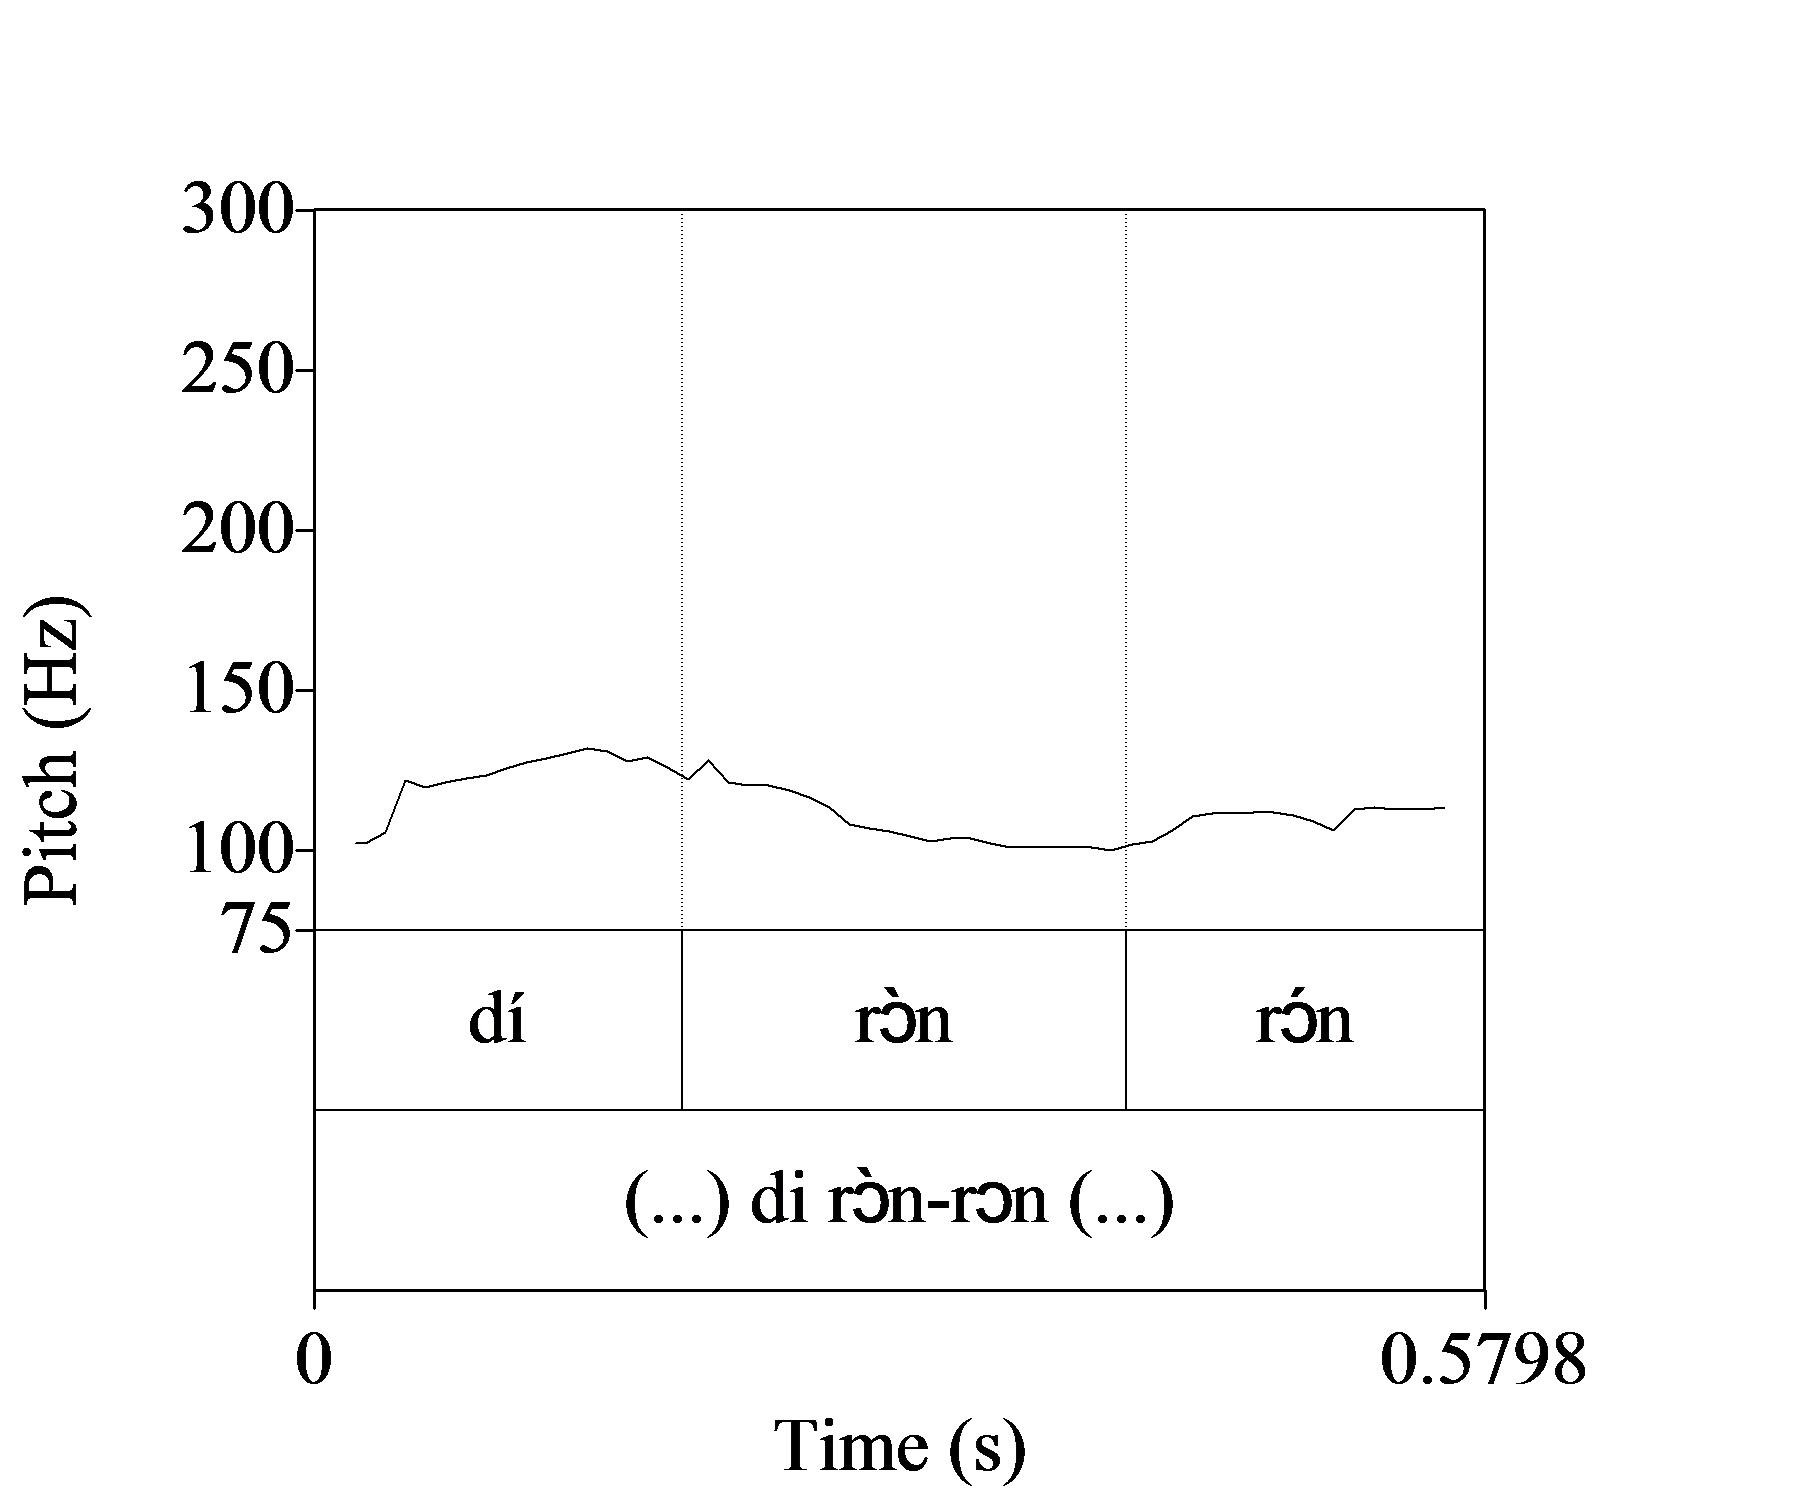
\includegraphics[height=.3\textheight]{figures/yakpomod-img23.png}
\end{figure}

\begin{figure}
\caption{Bisyllabic reduplicated verb}
\label{fig:key:3.22} 
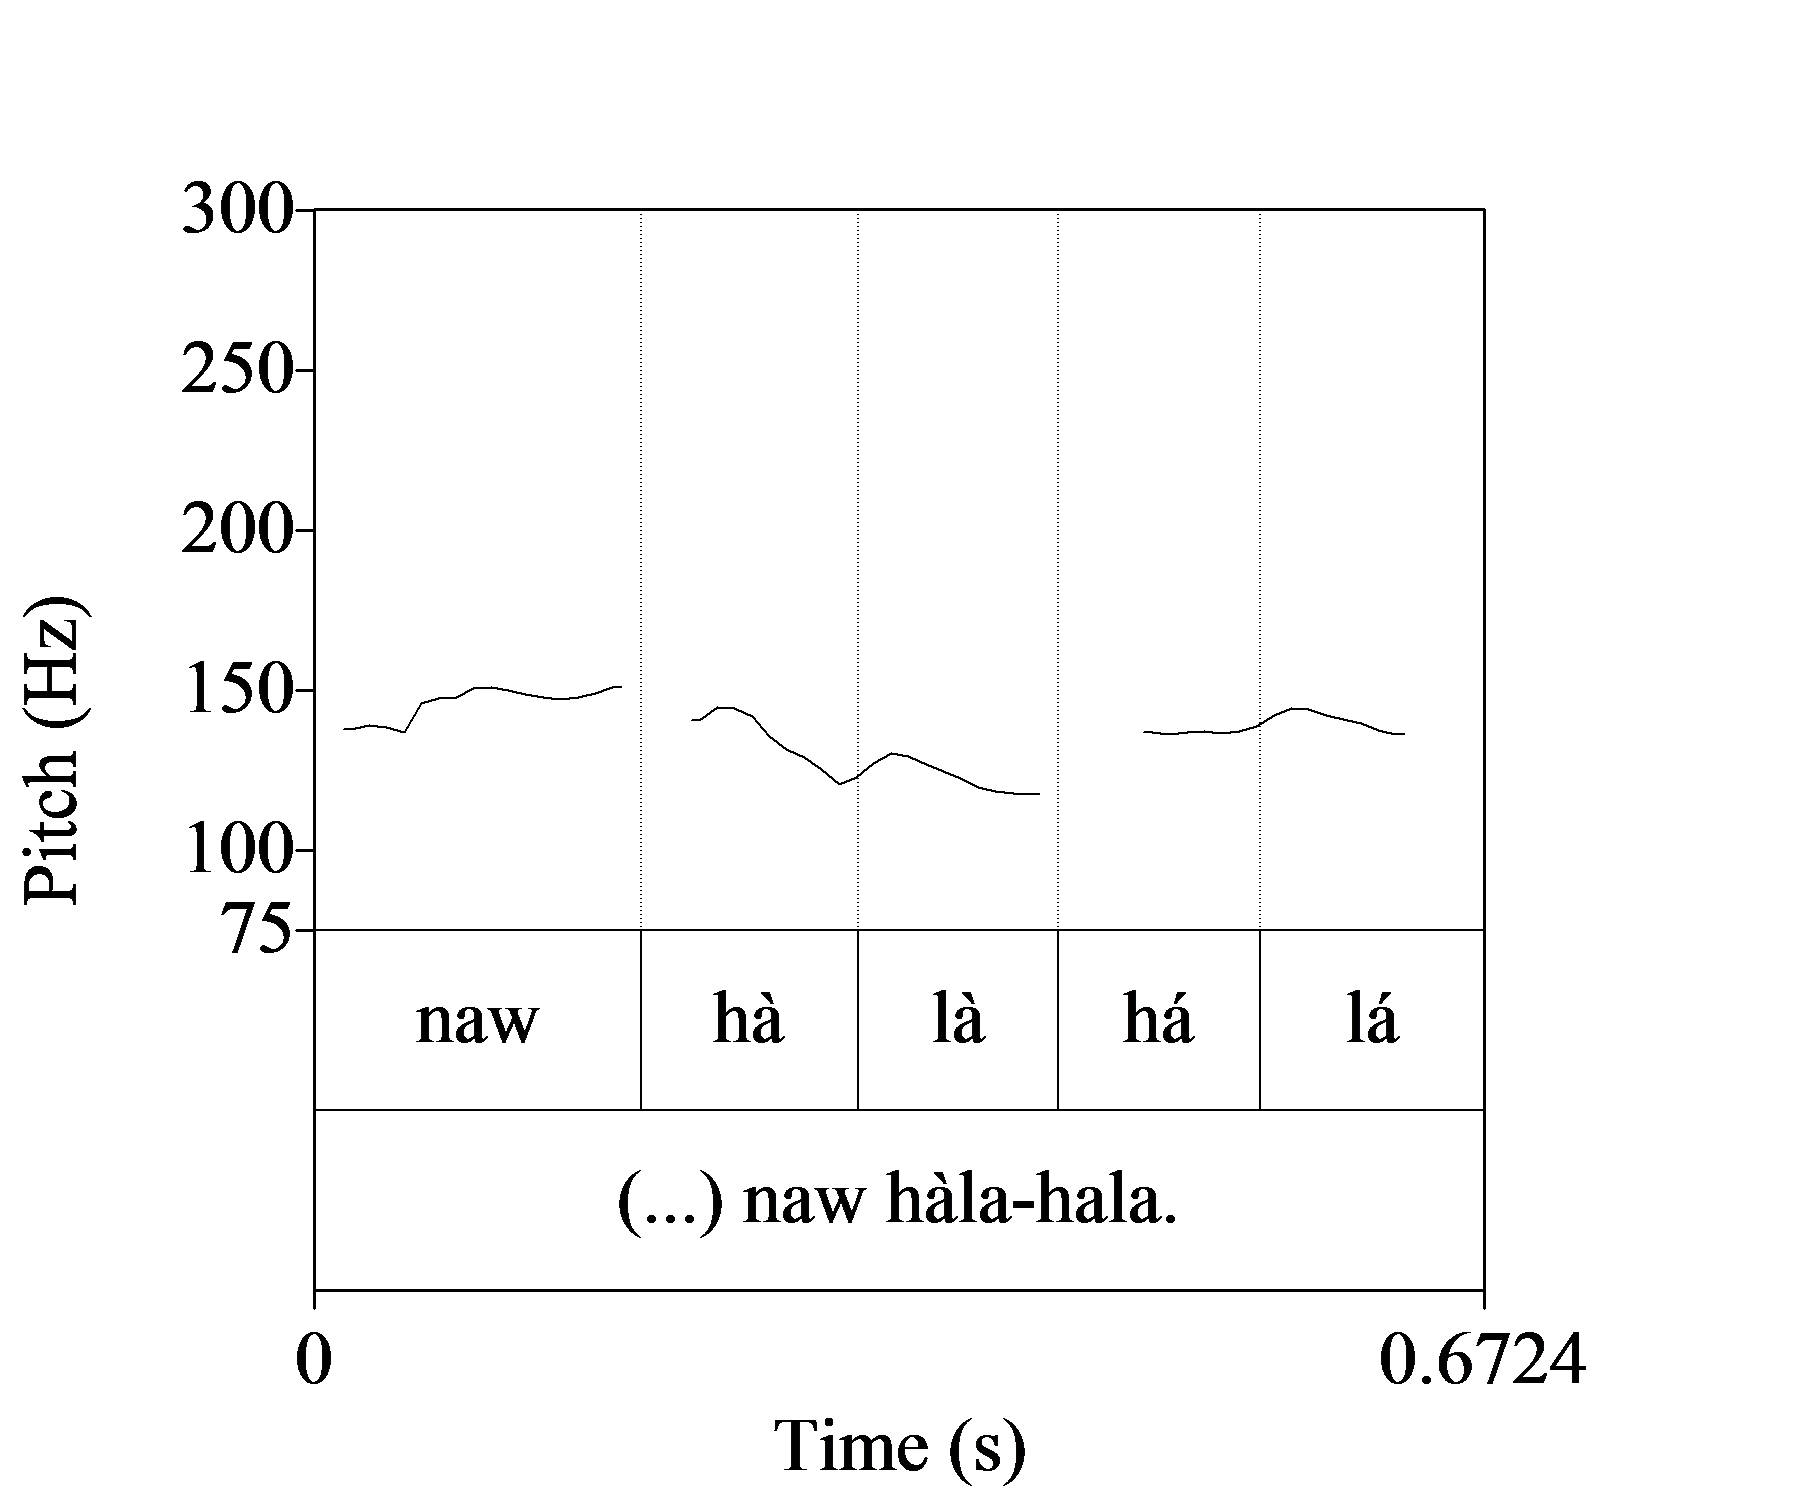
\includegraphics[height=.3\textheight]{figures/yakpomod-img24.png} 
\end{figure}
 
\ea%60
    \label{ex:key:60}
    \gll   Dí  \textstylePichiexamplebold{rɔn-}rɔ́n (…)\\
\textsc{h}  \textstylePichiexamplebold{\textsc{l}}\textsc{{}-h}\\
this  \textsc{red.cpd-}run\\
\glt ‘This running around (…)’
\z

\ea
	\label{ex:key:61}
\gll    Náw    \textstylePichiexamplebold{hala}{}-hála.\\
\textsc{h}    \textstylePichiexamplebold{\textsc{l}}\textstylePichiexamplenumberZchnZchn{.}\textstylePichiexamplenumberZchnZchn{\textsc{l}}\textsc{{}-h.h}\\
now    \textsc{red.cpd}{}-shout\\
\glt ‘Now, (it was) constant shouting.’\\
\z

\subsection{Pitch range expansion}\label{sec:3.2.5}

In Pichi, certain phonetic features may increase the prominence of a (series of) syllable(s). Segments may be lengthened or may be pronounced with increased volume, they may be pronounced with a breathy or creaky voice, and the speech rate may be slowed down or accelerated for stylistic effect. But there is no stress in Pichi in the sense of an automatic, metrically conditioned culmination of phonetic features as in intonation-only languages. Nor does Pichi make use of intonational melodies spanning the entire (or parts of the) utterance for the realisation of pragmatic functions, since these would override the lexical tone of individual words. Instead, pitch range expansion, and an extra-high tone in particular, are exploited to signal focus and emphasis. Focused or emphasised constituents may bear a higher than usual pitch, an extra-high tone on their H-toned syllable(s). The extra-high tone may spread rightwards onto following L-toned syllables until the word boundary is reached (cf. \sectref{sec:3.2.1}). 

\figref{fig:key:3.23} features the clefted verb \textit{drɔ́ngo} ‘be dead drunk’. In the pitch trace, the emphatic character of the predicate cleft construction \is{predicate cleft}is evident in two ways. The H-toned syllable of \textit{drɔ́ngo} bears an extra-high tone, and the segment /r/ is lengthened for emphasis. The utterance in \figref{fig:key:3.23} shades off into a chuckle from the fifth syllable onwards, which produces a wavering pitch trace:

\begin{figure}
\caption{Predicate cleft and extra-high tone for emphasis}
\label{fig:key:3.23}
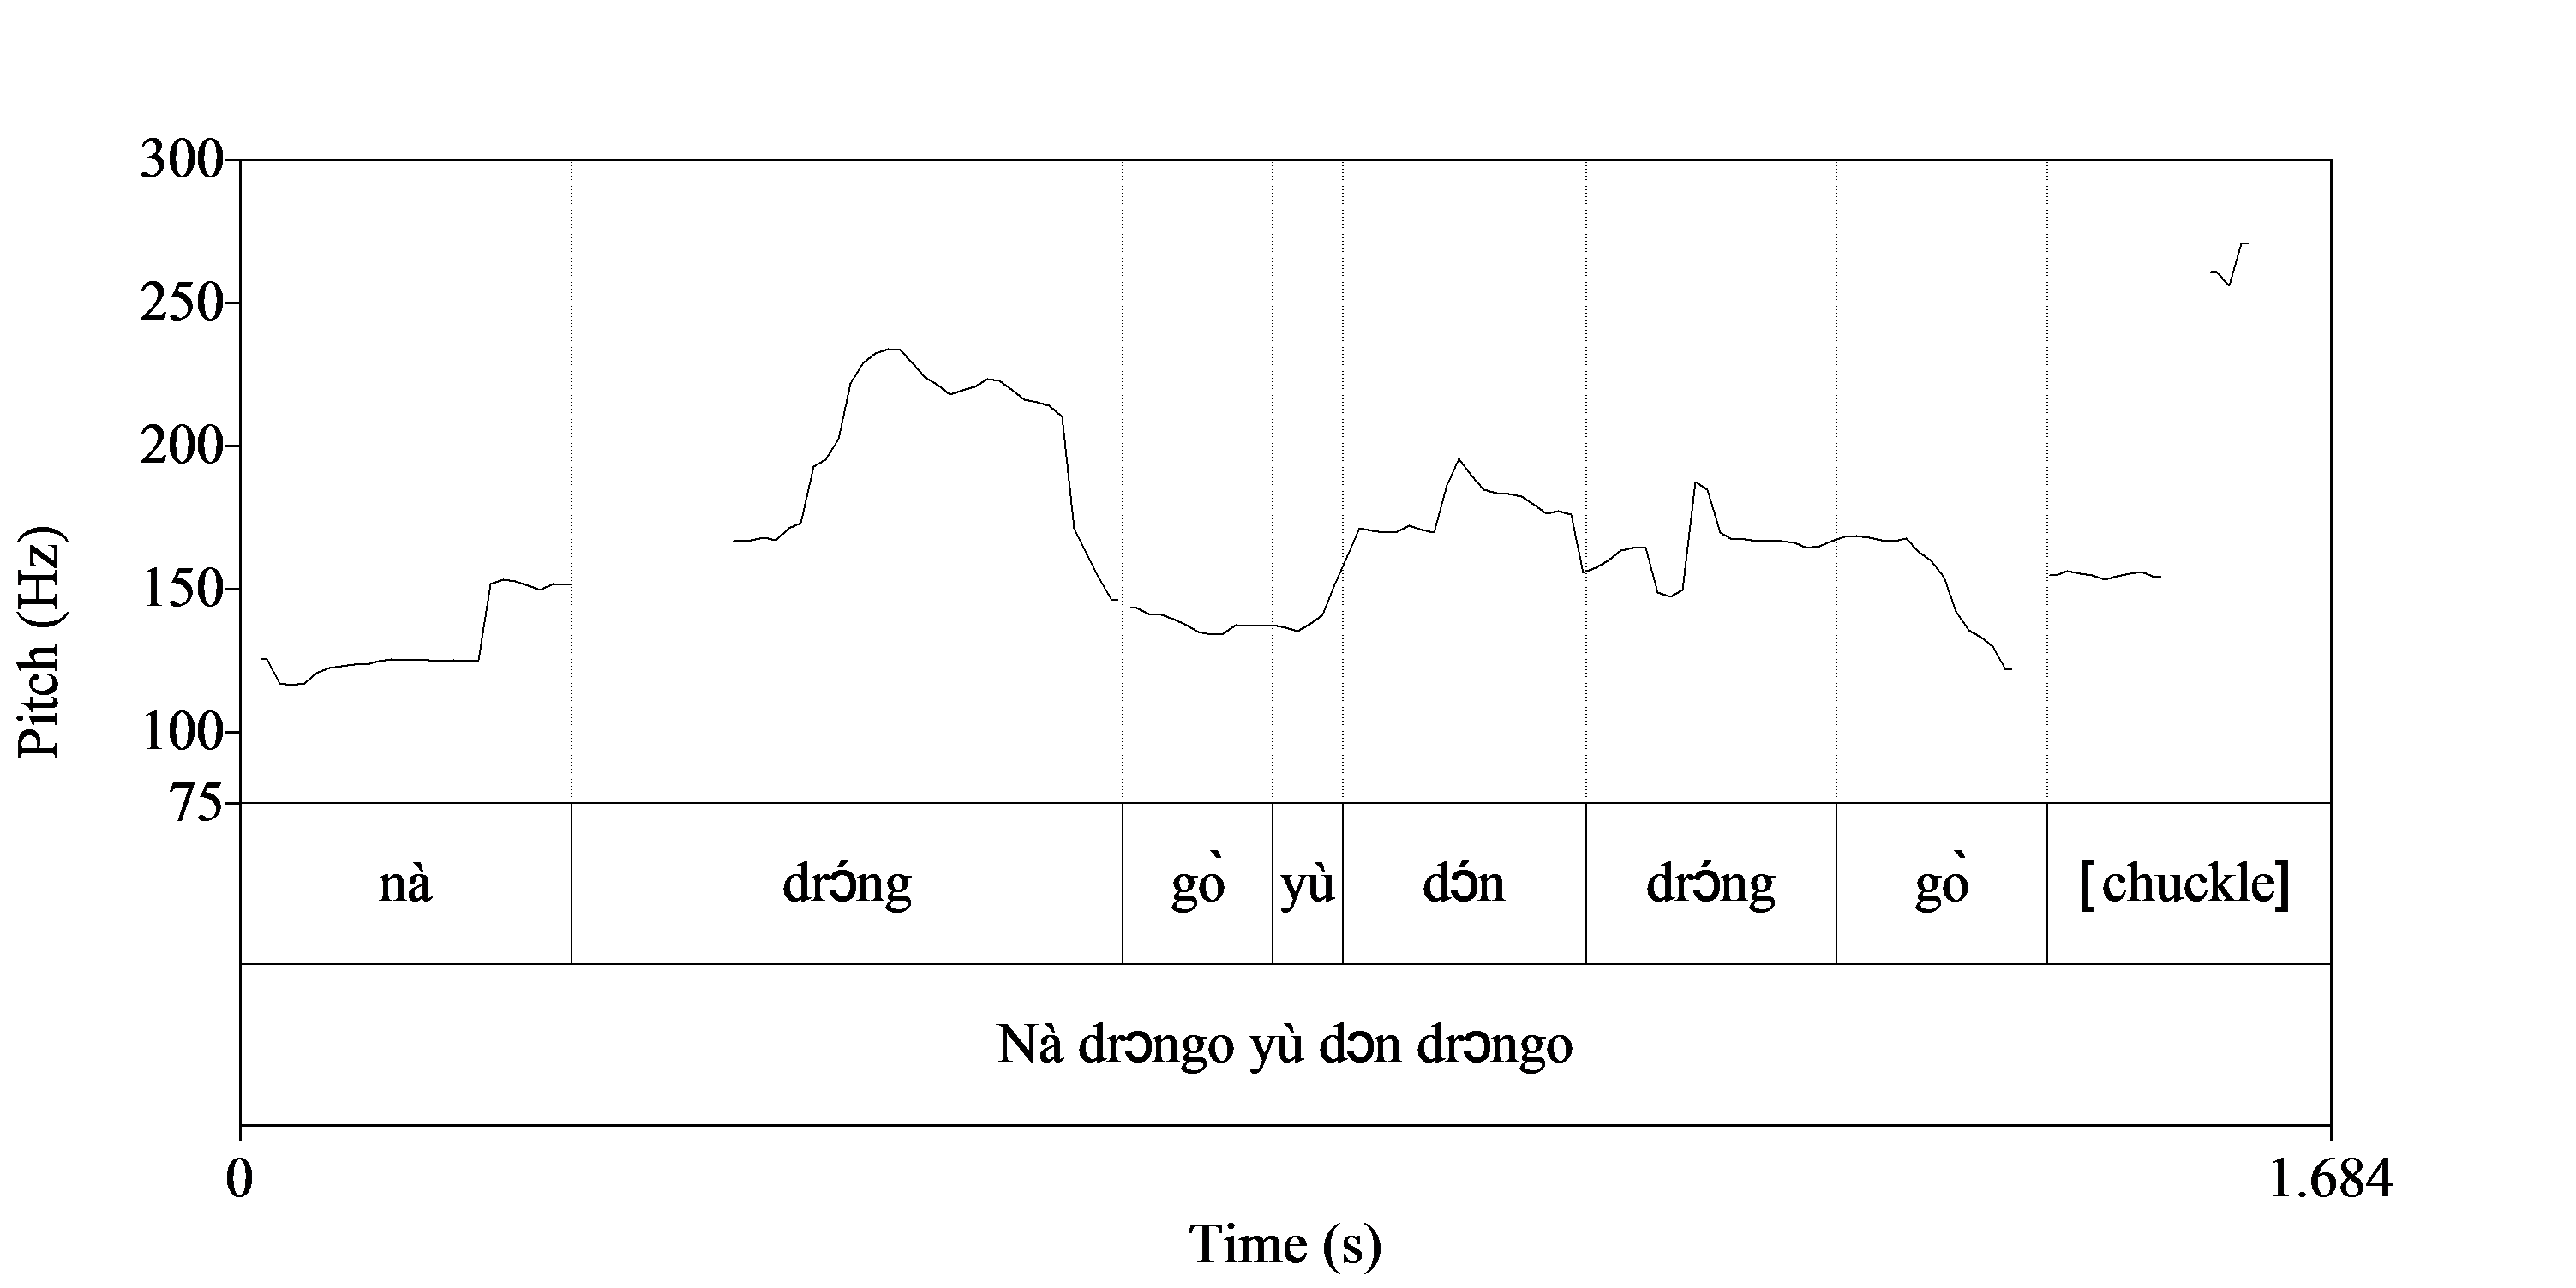
\includegraphics[height=.3\textheight]{figures/yakpomod-img25.png}
\end{figure}
 


\ea%62
    \label{ex:key:62}
    \glll   Na  [\textstylePichiexamplebold{drrrɔ́ngò}]    yu  dɔ́n  drɔ́ngo. \\
\textsc{l}  \textbf{\textsc{+h}}\textsc{.l}        \textsc{l}  \textsc{h}  \textsc{h.l}\\
\textsc{foc}  be.dead.drunk  \textsc{2sg}  \textsc{prf}  be.dead.drunk\\
\glt ‘You’re absolutely dead drunk.’     
\z

Elements that fulfil central functions in pragmatically marked contexts are particularly common with extra-high tone, e.g. question elements like \textit{háw} ‘how’, \textit{wétin} ‘what’, \textit{údat} ‘who’, \textit{ús=tín}  ‘what’, the negator \textit{nó}\is{negation}, modifications of degree via repetition\is{repetition} like \textit{bíg bíg} ‘very big’, and the degree adverb \textit{bád} ‘bad, extremely’. Both components of the repetition \textit{bíg bíg} ‘be very big’ in \figref{fig:key:3.24} below carry an extra-high tone. There is no sign of downstep\is{downstep} within the reduplicated sequence: 

\begin{figure}
\caption{Extra-high tone}
\label{fig:key:3.24}
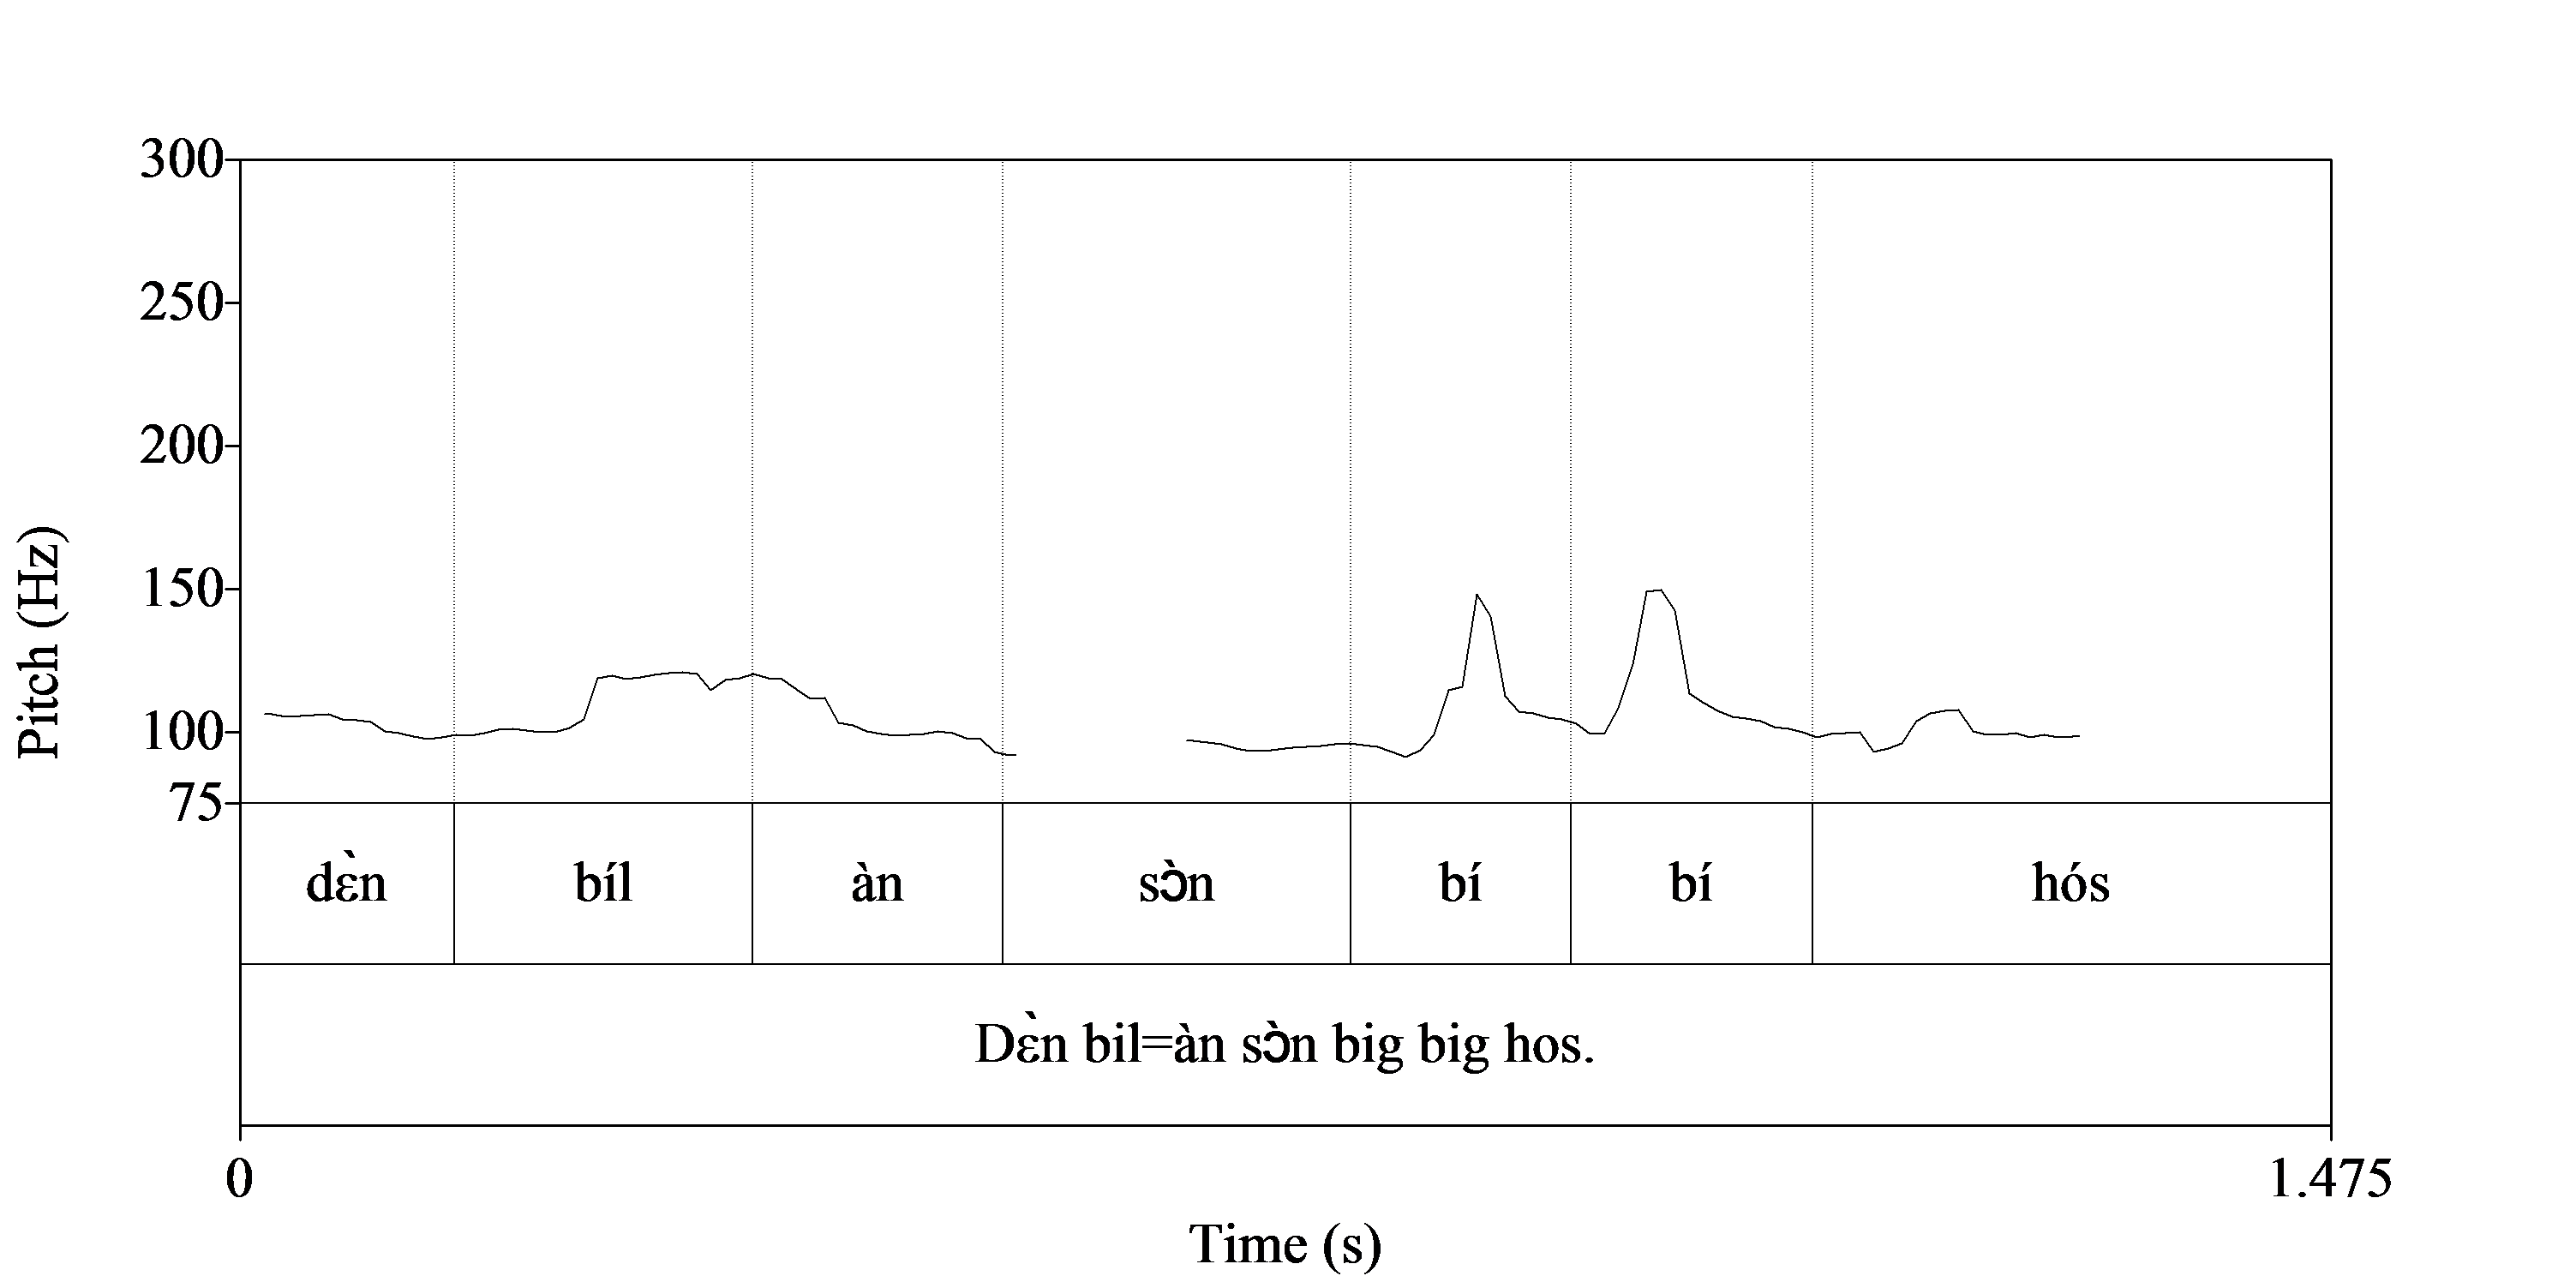
\includegraphics[height=.3\textheight]{figures/yakpomod-img26.png}
\end{figure}
 


\ea%63
    \label{ex:key:63}
    \glll   Dɛn    bíl=an    sɔn    \textstylePichiexamplebold{bíg}  \textstylePichiexamplebold{bíg}    hós.\\
\textsc{h}    \textsc{h=l}      \textsc{l}    \textbf{\textsc{+h}  \textbf{+h}}    \textsc{h}\\
\textsc{3pl}    build=\textsc{3sg.obj}  some  big  \textsc{rep}    house\\
\glt ‘They built him a huge house.’    
\z

Entire clauses or sentences may also be placed under focus \is{prosodic focus} by (a series of) extra-high tones, which thereby (cumulatively) fulfil(s) the same function as emphatic intonation covered in \sectref{sec:3.4.2} further below. There are two principal means of emphasising sentences, which are often used together. The last H tone of the utterance may be raised to an extra-high pitch as in \figref{fig:key:3.25}. Here the H tone of the utterance-final word \textit{mán} ‘man’ has been raised to an extra-high level. The sentence nonetheless bears declarative intonation. The word \textit{mán} still exhibits the utterance-final fall characteristic of declarative intonation (cf. \sectref{sec:3.4.1}) but at a significantly higher pitch level than in a non-emphatic context:

\begin{figure}
\caption{Utterance-final extra-high tone for emphasis\is{emphasis}}
\label{fig:key:3.25}
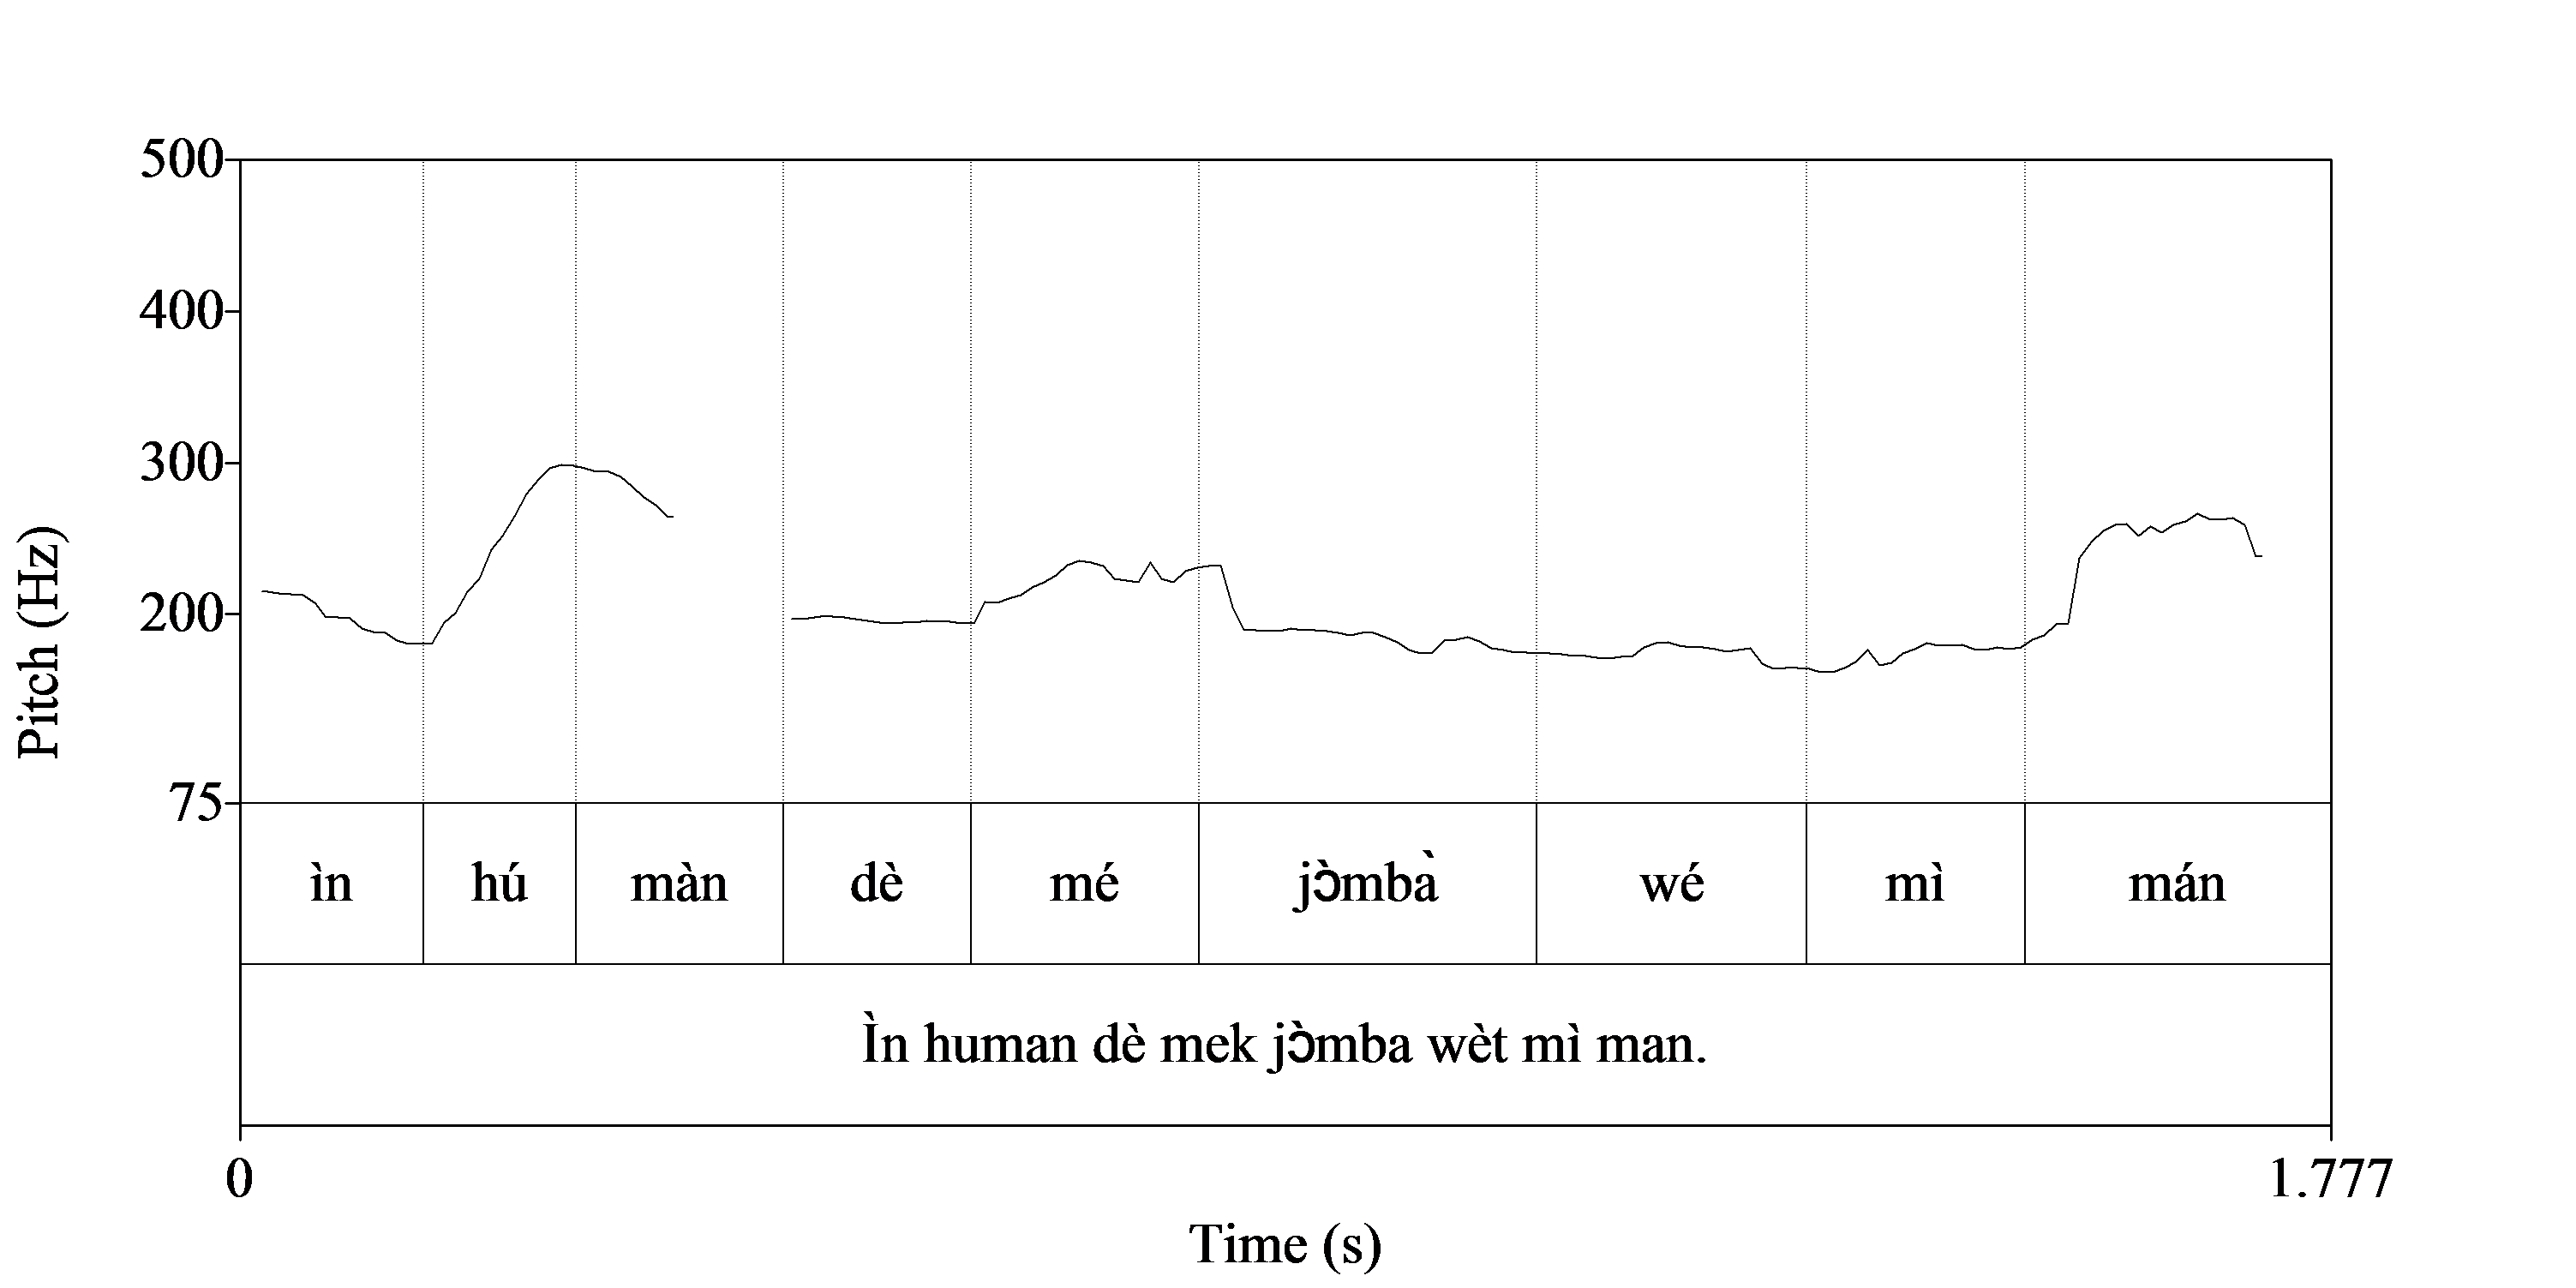
\includegraphics[height=.3\textheight]{figures/yakpomod-img27.png}
\end{figure}
 


\ea%64
    \label{ex:key:64}
    \glll   Yu  húman  de  mék    jɔmba  wet  mi    \textstylePichiexamplebold{mán}.\\
\textsc{l}  \textsc{h.l}    \textsc{l}  \textsc{h}    \textsc{l.l}    \textsc{l}  \textsc{l}    \textbf{\textsc{+h}}\textsc{l\%}\\
\textsc{2sg}  woman  \textsc{ipfv}  make  affair  with  \textsc{1sg.poss}  man.\\
\glt ‘Your wife is having an affair with my husband.’
\z

Secondly, the use of an utterance-final extra-high tone is often accompanied by “pitch range expansion” \citep[276]{Yip2002}. Alternatively, pitch range expansion may be accompanied by the use of the emphatic boundary tone instead of the utterance-final extra-high tone (cf. \sectref{sec:3.4.2}). During pitch range expansion, the pitch range between H and L tones is widened throughout the entire utterance by pronouncing H tones with a higher-than-usual pitch and, optionally, L tones with a lower-than-usual pitch. This creates a strongly undulating pitch contour over the entire utterance.

\figref{fig:key:3.26} graphically depicts the dramatic rises and falls that may characterise pitch range expansion. The female speaker begins with an L-toned \textit{na} at 190 Hz, rises to 490 Hz with H-toned \textit{só}, then falls to an all-time low with \textit{dɛn} at 145 Hz, until the pitch range gradually evens out towards the end of the utterance:

\begin{figure}
\caption{Pitch range expansion for emphasis\is{emphasis}}
\label{fig:key:3.26}
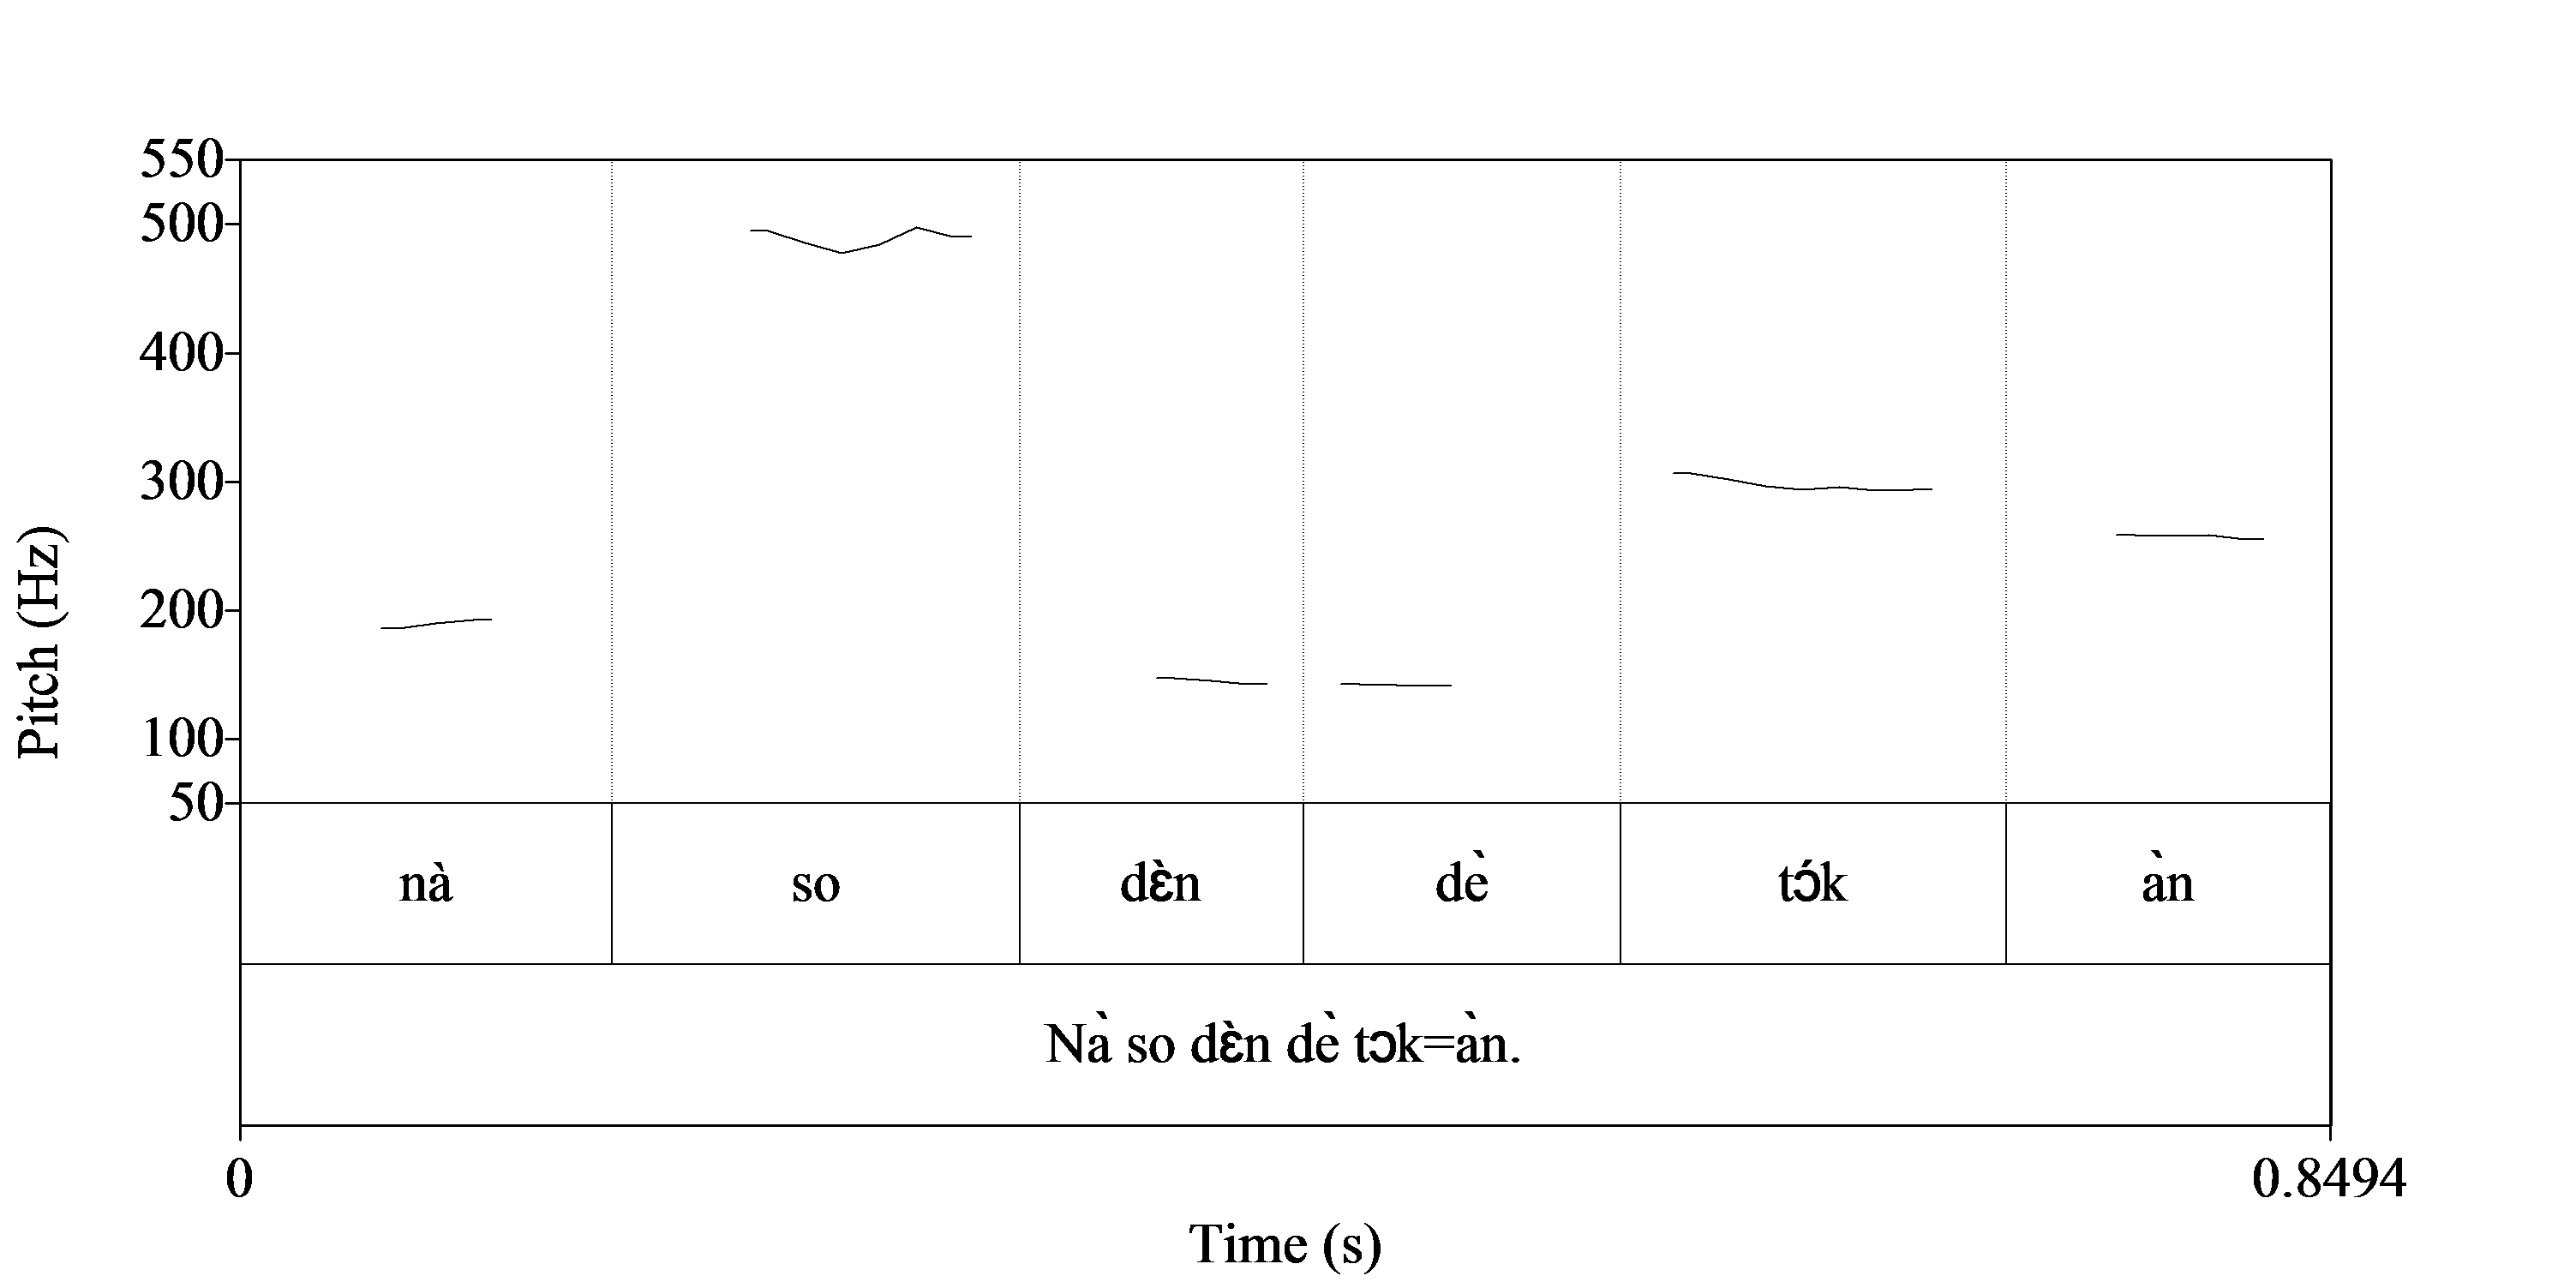
\includegraphics[height=.3\textheight]{figures/yakpomod-img28.png}
\end{figure}
 


\ea%65
    \label{ex:key:65}
    \glll   Na  \textstylePichiexamplebold{só}    \textbf{dɛn}  \textbf{de}  \textbf{tɔ́k}=an.    \\
\textsc{l}  \textbf{\textsc{+h}    \textbf{+l}  \textbf{+l}  \textbf{+h}}\textsc{=lh\%}      \\
\textsc{foc}  like.that  \textsc{3pl}  \textsc{ipfv}  talk=\textsc{3sg.obj}\\
\glt ‘That’s how they say it.’
\z

\section{Tone-conditioned suppletive allomorphy}\label{sec:3.3}

Pichi features a tone-conditioned suppletive allomorphy (TCSA) of the two pronominal variants \textit{=an} \textsc{‘3sg.obj’} and \textit{ín} ‘\textsc{3sg.indp’}, which may both instantiate (direct and indirect) object case (cf. \sectref{sec:5.4.1} for an overview of the inflection of personal pronouns). Suppletive allomorphy is conditioned by a tonotactic prohibition of immediately adjoining or “string-adjacent” \citep{Suzuki1998} identical tones (cf. also \sectref{sec:2.6.2.2}). Suppletive allomorphy therefore relies on the conditioning environment of vowel hiatus. Further, there are no phonemic long vowels in Pichi. String-adjacent vowels within the same lexical word are always heterosyllabic, and in addition, invariably carry polar tones (cf. \sectref{sec:2.6.2.2}). TCSA can therefore only be triggered when the enclisis of \textit{=an} \textsc{‘3sg.obj’} creates a phonological word. A head with an L-toned vowel-final syllable may therefore not take the vowel-initial L-toned clitic object pronoun \textit{=an}. Instead, the independent (emphatic) personal pronoun \textit{ín} \textsc{‘3sg.indp’} is recruited as a suppletive allomorph. Allomorph distribution according to the phonological class of the host is summarised in \tabref{tab:key:3.4}:

%%please move \begin{table} just above \begin{tabular
\begin{table}
\caption{Distribution of suppletive object pronouns}
\label{tab:key:3.4}

\begin{tabularx}{.8\textwidth}{XXl}
\lsptoprule
{Host class} & {Allomorph} & {Example}\\
\midrule
C/{\longrule}\# & =an & [márè\textbf{d}=àn]\\
\'{V}/{\longrule}\# & =an & [tròw\textbf{é}=àn]\\
\`{V}/{\longrule}\# & ín & [fíb\textbf{à} ín]\\
\lspbottomrule
\end{tabularx}
\end{table}

There is no tonotactic restriction on the enclisis of \textit{=an} with consonant-final hosts like \textit{máred} ‘marry’, since the condition of tonal string-adjacency is not met: 


\ea%66
    \label{ex:key:66}
    \gll   E    go  máre\textbf{d}=\textbf{an}.\\
\textsc{3sg.sbj}  \textsc{pot}  marry=\textsc{3sg.obj}\\

\glt ‘S/he’ll marry him/her.’ 
\z

There are no restrictions on the enclisis of \textit{=an} with vowel-final hosts with a word-final H-tone like \textit{trowé} ‘throw, pour away’, since the vowel sequence across the morpheme boundary bears a polar [H.L] tone:


\ea%67
    \label{ex:key:67}
    \gll   A    fít  ték    di  wɔtá  a    trow\textbf{é}=\textbf{an}.\\
\textsc{1sg.sbj}  can  take    \textsc{def}  water  \textsc{1sg.sbj}  throw=\textsc{3sg.obj}\\

\glt ‘I can take the water (and) pour it away.’ 
\z

If the word-final vowel of the host is L-toned, as with \textit{fíba} ‘resemble’, the pitch configuration after enclisis of \textit{=an} across the clitic boundary would be [L.L]. This is an illicit pitch configuration over string-adjacent vowels in Pichi phonological words and triggers the use of suppletive \textit{ín} ‘\textsc{3sg.indp’.} Compare the following two examples:


\ea%68
    \label{ex:key:68}
    \gll   \textit{*}Yu    fíb\textbf{a}=\textbf{an}    bɔkú.\\
\textsc{2sg}  resemble=\textsc{3sg.obj}  a.lot\\

\glt  ‘You resemble him a lot.’ 
\z


\ea%69
    \label{ex:key:69}
    \gll   Yu  \textbf{fíba}      \textbf{ín}    bɔ́ku.\\
\textsc{2sg}  resemble    \textsc{3sg.indp}  a.lot\\

\glt ‘You resemble him/her a lot.’ 
\z

The class of words that features the allomorph \textit{ín} as an object pronoun also includes verbs of Spanish origin. Spanish verbs are always inserted into Pichi clauses in the Spanish \textsc{3sg} present tense form, irrespective of their tense-aspect (cf. \sectref{sec:13.2.2}). Examples follow with the verbs \textit{fírma} ‘sign’ (< Span. \textit{firmar}) from the Spanish 1\textsuperscript{st} conjugation class, and \textit{sube} ‘go/bring up’ (< Span. \textit{subir}) from the 3\textsuperscript{rd} conjugation class:


\ea%70
    \label{ex:key:70}
    \gll   Dɛn    nó    \textbf{fírma}  \textbf{ín}    yét.    \\
\textsc{3pl}    \textsc{neg}    sign    \textsc{3sg.indp}  yet\\


\glt ‘They haven't signed it yet.’\\

\z

\ea%71
    \label{ex:key:71}
    \gll   Dán    mán    go  \textbf{súbe}  \textbf{ín}.\\
that    man    \textsc{pot}  bring.up  \textsc{3sg.indp}\\

\glt ‘That man will bring it [the suitcase] up.’
\z

Pichi has a second mechanism next to tone-conditioned suppletive allomorphy to ensure that the requirement of a string-adjacent polar [H.L] tone is not breached. A buffer consonant /r/ can be inserted at the clitic boundary. Epenthesis forestalls the cross-morphemic vowel hiatus and makes the use of the allomorph \textit{ín} unnecessary:


\ea%72
    \label{ex:key:72}
    \gll   Yu  fíba[\textbf{r}]=\textbf{an}    bɔkú.\\
\textsc{2sg}  resemble=\textsc{3sg.obj}  a.lot\\

\glt ‘You resemble him a lot.’ 
\z

Once the epenthetic segment is present, there is no phonotactic difference with a word in which the final consonant forms an integral part of the root like \textit{máred} ‘marry’ in \REF{ex:key:66}. Another example featuring epenthesis follows, involving the general associative preposition \textit{fɔ} ‘\textsc{prep}’. In \REF{ex:key:73}, we find /r/ epenthesis, in \REF{ex:key:74}, suppletive allomorphy:


\ea%73
    \label{ex:key:73}
    \gll   E    tót=an    fɔ[\textbf{r}]=\textbf{an}.\\
\textsc{3sg.sbj}  carry=\textsc{3sg.obj}  \textsc{prep=3sg.obj}\\

\glt ‘He carried it for her.’
\z


\ea%74
    \label{ex:key:74}
    \gll   Dán    tín    dé    \textbf{fɔ}  \textbf{ín}.\\
that    thing  \textsc{be.loc}  \textsc{prep}  \textsc{3sg.indp}\\

\glt ‘That thing is hers.’
\z

Three aspects are noteworthy with respect to /r/ epenthesis in Pichi. Firstly, /r/ insertion is exceedingly rare in natural discourse. In the Pichi corpus, there are less than a dozen instances of /r/ epenthesis in natural discourse, involving a mere handful of lexemes, among them \textit{kɔ́ba[r]=an} ‘cover it’, \textit{klía[r]=an} ‘clear it’, \textit{fía[r]=an} ‘fear him/her’, \textit{fíba[r]=an} ‘resemble him/her, \textit{drɔ́ngo[r]=an} ‘get him/her drunk’, and \textit{fɔ[r]=an} ‘for him/her’. By contrast, the corpus contains hundreds of syntagmas involving the suppletive allomorph \textit{ín.} I could therefore only uncover the distribution of the epenthetic /r/ and its role in TCSA by means of elicitation. Secondly, elicitation revealed that the availability of /r/ epenthesis is subject to considerable idiolectal variation. For some speakers, the use of epenthesis with many verbs is not acceptable, i.e. *\textit{fála[r]=an} ‘follow him/her’, for others it is. All speakers, however, accepted TCSA with all verbs and prepositions, whether belonging to the native Pichi or the non-native Spanish lexical layer. 


The third aspect of interest is that /r/ epenthesis is ungrammatical with Spanish derived verbs, cf. \REF{ex:key:75}. Epenthesis is limited to the native layer of the Pichi vocabulary, thus excluding inserted Spanish verbs from the application of /r/ epenthesis, and limiting them to TCSA alone, hence the ungrammaticality of the following example.



\ea[*]{%75
    \label{ex:key:75}
    \gll   Yu  gɛ́t    fɔ  fírma[r]=an.\\
 \textsc{2sg}  get    \textsc{prep}  sign=\textsc{3sg.obj}\\
\glt ‘You have to sign it.’
}\z

Pichi words with a word-final L-toned /ì/, e.g. \textit{wɔ́ri} ‘worry’, merit some attention in the context of epenthesis. Such words exhibit the conditioning feature but neither trigger /r/ epenthesis nor TCSA, compare the ungrammatical sentences \REF{ex:key:76} and \REF{ex:key:77}. Other verbs in this group are \textit{sɔ́ri} ‘feel sorry’, \textit{grídi} ‘be greedy’, \textit{hángri} ‘be hungry’, \textit{lési} ‘be lazy’, and \textit{tɔ́sti} ‘be thirsty’. 


\ea[*]{%76
    \label{ex:key:76}
    \gll   Dɛn  wɔ́ri[\textbf{r}]=\textbf{an}    bɔkú. \\
 \textsc{3pl}    worry=\textsc{3sg.obj}    much\\
\glt ‘They worried him a lot.’
}\z


\ea[*]{%77
    \label{ex:key:77}
    \gll   Dɛn  wɔ́ri    \textbf{ín}    bɔkú.  \\
\textsc{3pl}    worry  \textsc{3sg.indp}  much\\
\glt ‘They worried him a lot.’ 
}\z

Instead, a word-final nasal /n/ appears at the clitic boundary, thus avoiding the LL vowel hiatus that should trigger suppletive allomorphy, as in \REF{ex:key:78}:


\ea%78
    \label{ex:key:78}
    \gll   Di  tín    sɔ́rin=an         bɔkú.   \\
\textsc{def}  thing  make.sorry=\textsc{3sg.obj}  much\\

\glt ‘This made her feel very sorry.’
\z

Outside of the clitic environment, the wordfinal /ì/ in these words may, but need not be pronounced as a nasalised vowel, as shown in the phonetic transcription in \REF{ex:key:79}:


\ea%79
    \label{ex:key:79}
    \gll   A    sɔ́ri  [\textbf{sɔ́rĩ\`{} }]  sé    e    kíl  di  dɔ́g.\\
\textsc{1sg.sbj}  feel.sorry  \textsc{quot}    \textsc{3sg.sbj}  kill  \textsc{def}  dog\\

\glt ‘I felt sorry that she killed the dog.’
\z

The word-final /n/ in examples like \REF{ex:key:79} is therefore not epenthetic. It is morphologically affiliated to the verbal root and is realised in the clitic environment. The word-final /n/ in verbs like \textit{sɔ́ri} (group 1) has been constructed by analogy with words like \textit{físin} ‘(to) fish’, \textit{hɔ́ntin} ‘(to) hunt’, \textit{mɔ́nin} ‘morning’, \textit{ívin} ‘evening’, and \textit{plantí} ‘plantain’ (group 2). The construction of a word-final /n/ in group 1 words probably occurred in response to the ban on string-adjacent identical tones in the context of cliticisation.

\section{Intonation}\label{sec:3.4}

The functions of intonation are realised by sentence-final particles and utterance-final boundary tones. Pichi boundary tones are floating tones, which are inserted at the right edge of an utterance. These boundary tones serve pragmatic functions by differentiating sentence types, such as declaratives from questions. They also fulfil grammatical functions by linking clauses.


Four boundary tones and contours, represented by <\%> \citep{Pierrehumbert1980}, were identified in the corpus. Their functions with declaratives and questions are summarised in \tabref{tab:key:3.5} (cf. Hirst \& Di \citealt{Cristo1998}:18–20):


%%please move \begin{table} just above \begin{tabular
\begin{table}
\caption{Utterance type and boundary tones}
\label{tab:key:3.5}

\begin{tabularx}{.8\textwidth}{XXl}
\lsptoprule

{Boundary tone} & {Declaratives} & {Questions}\\
\midrule
L\% & Non-emphatic & Content\\
LH\% (additive) & Emphatic & {}---\\
& List & {}---\\
${\emptyset}$\% (no tone) & Continuative & {}---\\
& Emphatic & {}---\\
LH\% (substitutive) & {}--- & Yes–no\\
\lspbottomrule
\end{tabularx}
\end{table}

A boundary (contour) tone (henceforth only “boundary tone”) associates with the last syllable of an utterance. A boundary tone (BT) may either form a contour by itself (e.g. question intonation) or arise if the lexical tone (LT) of the utterance-final syllable is polar to the following BT. Otherwise, a BT produces a fall or a level tone over the utterance-final syllable.

\tabref{tab:key:3.6} below shows how LTs and BTs interact. The leftmost column contains the word-final LT over the last syllable of the utterance. The top row contains the relevant BT. The boxes in the table contain the (contour) tones over the utterance-final syllable that result from the interaction of LT and BT. These tones represent the phonetic output, the way the tone is actually pronounced. Some of these output tones are level tones, others are contour tones of varying complexity:

%%please move \begin{table} just above \begin{tabular
\begin{table}
\caption{Interaction of lexical tones and boundary tones}
\label{tab:key:3.6}
\small
\begin{tabularx}{\textwidth}{lp{2cm}lXXX}
\lsptoprule

LT/BT & Example & Declarative

L\% & Emphatic LH\% & Cont./Emph.

${\emptyset}$\% & Question

LH\% \\
\midrule
\MakeUppercase{l} & \textit{dɛn} \textsc{‘3pl’} \newline \textit{Píchi} ‘Pichi’ 
\newline 
\MakeUppercase{l}    \MakeUppercase{h.l} & L (fall) & \MakeUppercase{LH} & L (level) & \MakeUppercase{lh}\\

\tablevspace
\MakeUppercase{h} & \textit{gó} ‘go’ \newline \textit{pikín}\textstyleTableEnglishZchn{ ‘child’}
\newline 
 \MakeUppercase{h}    \MakeUppercase{l.h} & HL & \MakeUppercase{hlh} & H & \MakeUppercase{lh}\\


\tablevspace
\MakeUppercase{h} & \textit{bɔbí} \textstyleTableEnglishZchn{‘breast’}
\newline 
\MakeUppercase{l.h} & H & \MakeUppercase{hlh} & H & \MakeUppercase{lh}\\
\lspbottomrule
\end{tabularx}
\end{table}

LTs are not overridden by BTs save in one instance. In yes–no questions\is{yes-no questions}, the utterance-final LT is deleted and replaced by the question boundary contour tone. This is why the rightmost column in \tabref{tab:key:3.6} features the same LH\% boundary tone in the utterance-final position with all tone classes. 

\subsection{Declarative intonation}\label{sec:3.4.1}

Non-emphatic declaratives feature an L\%, which is also found on the right edge of the citation form of words. The declarative L\% causes an utterance-final fall to the bottom of the pitch register. Compare the word-final L-toned syllable of \textit{kɔ́ntri} ‘country’ in \figref{fig:key:3.27}: 

\begin{figure}
\caption{Declarative L\% over H.L word}
\label{fig:key:3.27}
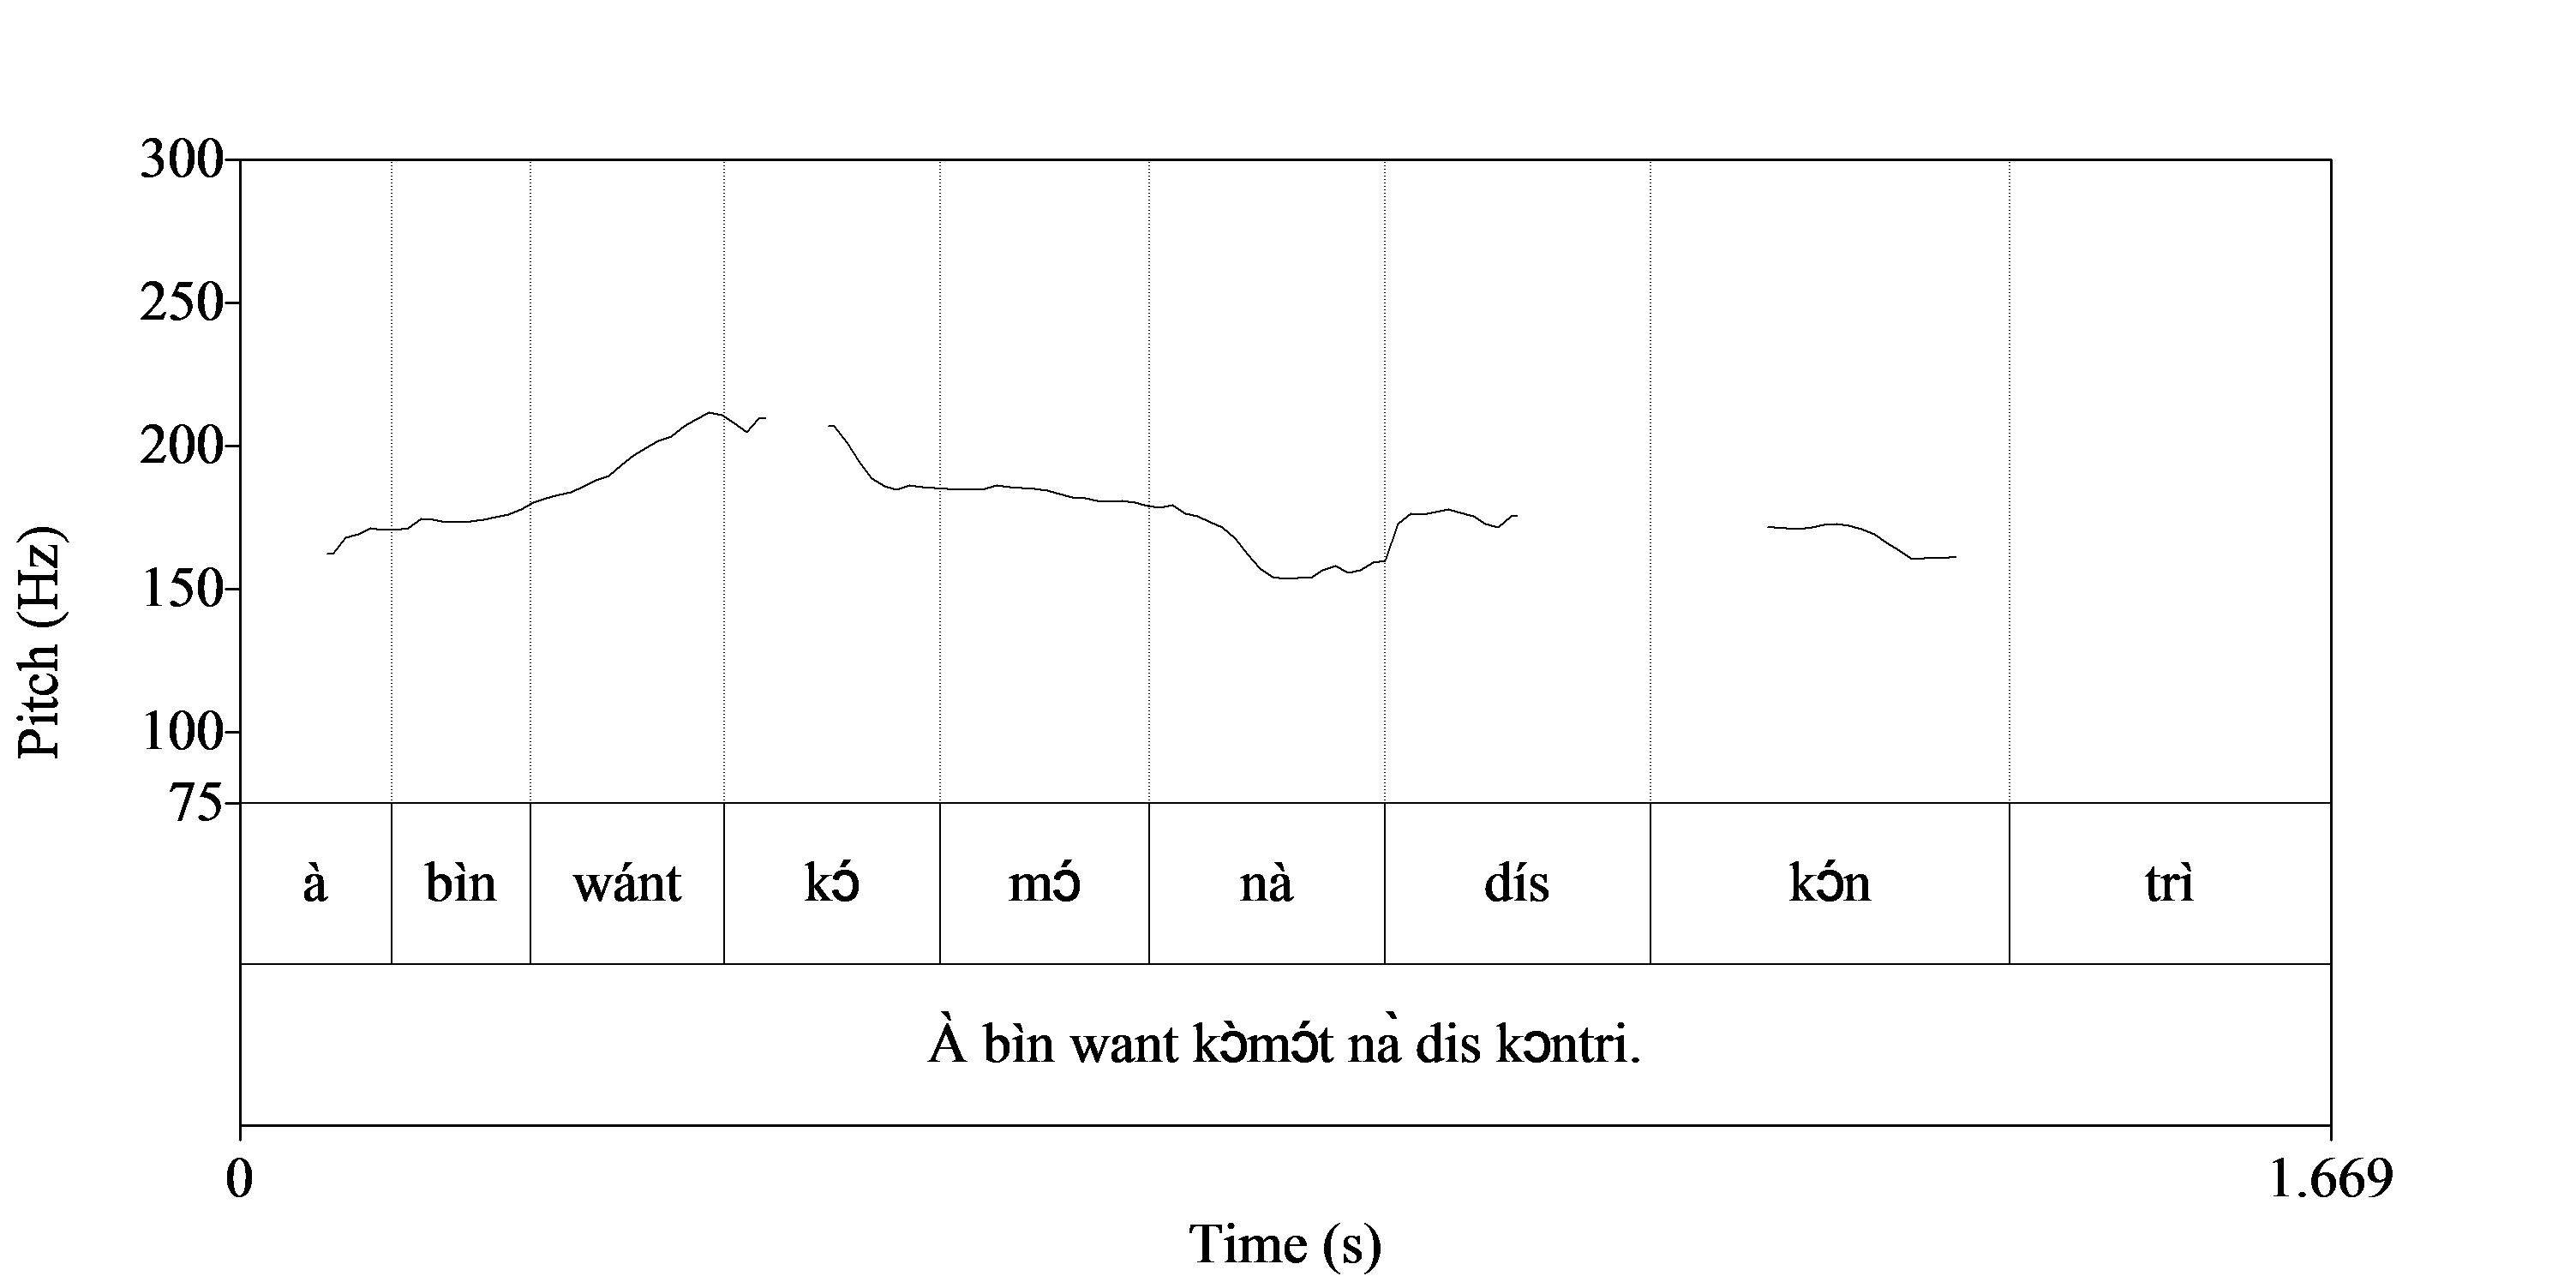
\includegraphics[height=.3\textheight]{figures/yakpomod-img29.png}
\end{figure}

%%[Warning: Draw object ignored]
 
\ea%80
    \label{ex:key:80}
    \glll   A    bin  wánt  kɔmɔ́t  na  dís  kɔ́ntri.\\
\textsc{l}    \textsc{l}  \textsc{h}    \textsc{l.h}    \textsc{l}  \textsc{h}  \textsc{h.l}\textbf{\textsc{l\%}}\\
\textsc{1sg.sbj}  \textsc{pst}  want  go.out  \textsc{loc}  this  country\\
\glt ‘I wanted to leave this country.’→  
\z

In contrast, polysyllabic vowel-final words with a final lexical H tone do not usually feature an utterance-final fall in non-emphatic declaratives. They retain their word-final H tone. Compare \textit{bɔbí} ‘breast’ in \figref{fig:key:3.28}: 

\begin{figure}
\caption{Unpronounced declarative L\% over L.H word}
\label{fig:key:3.28}
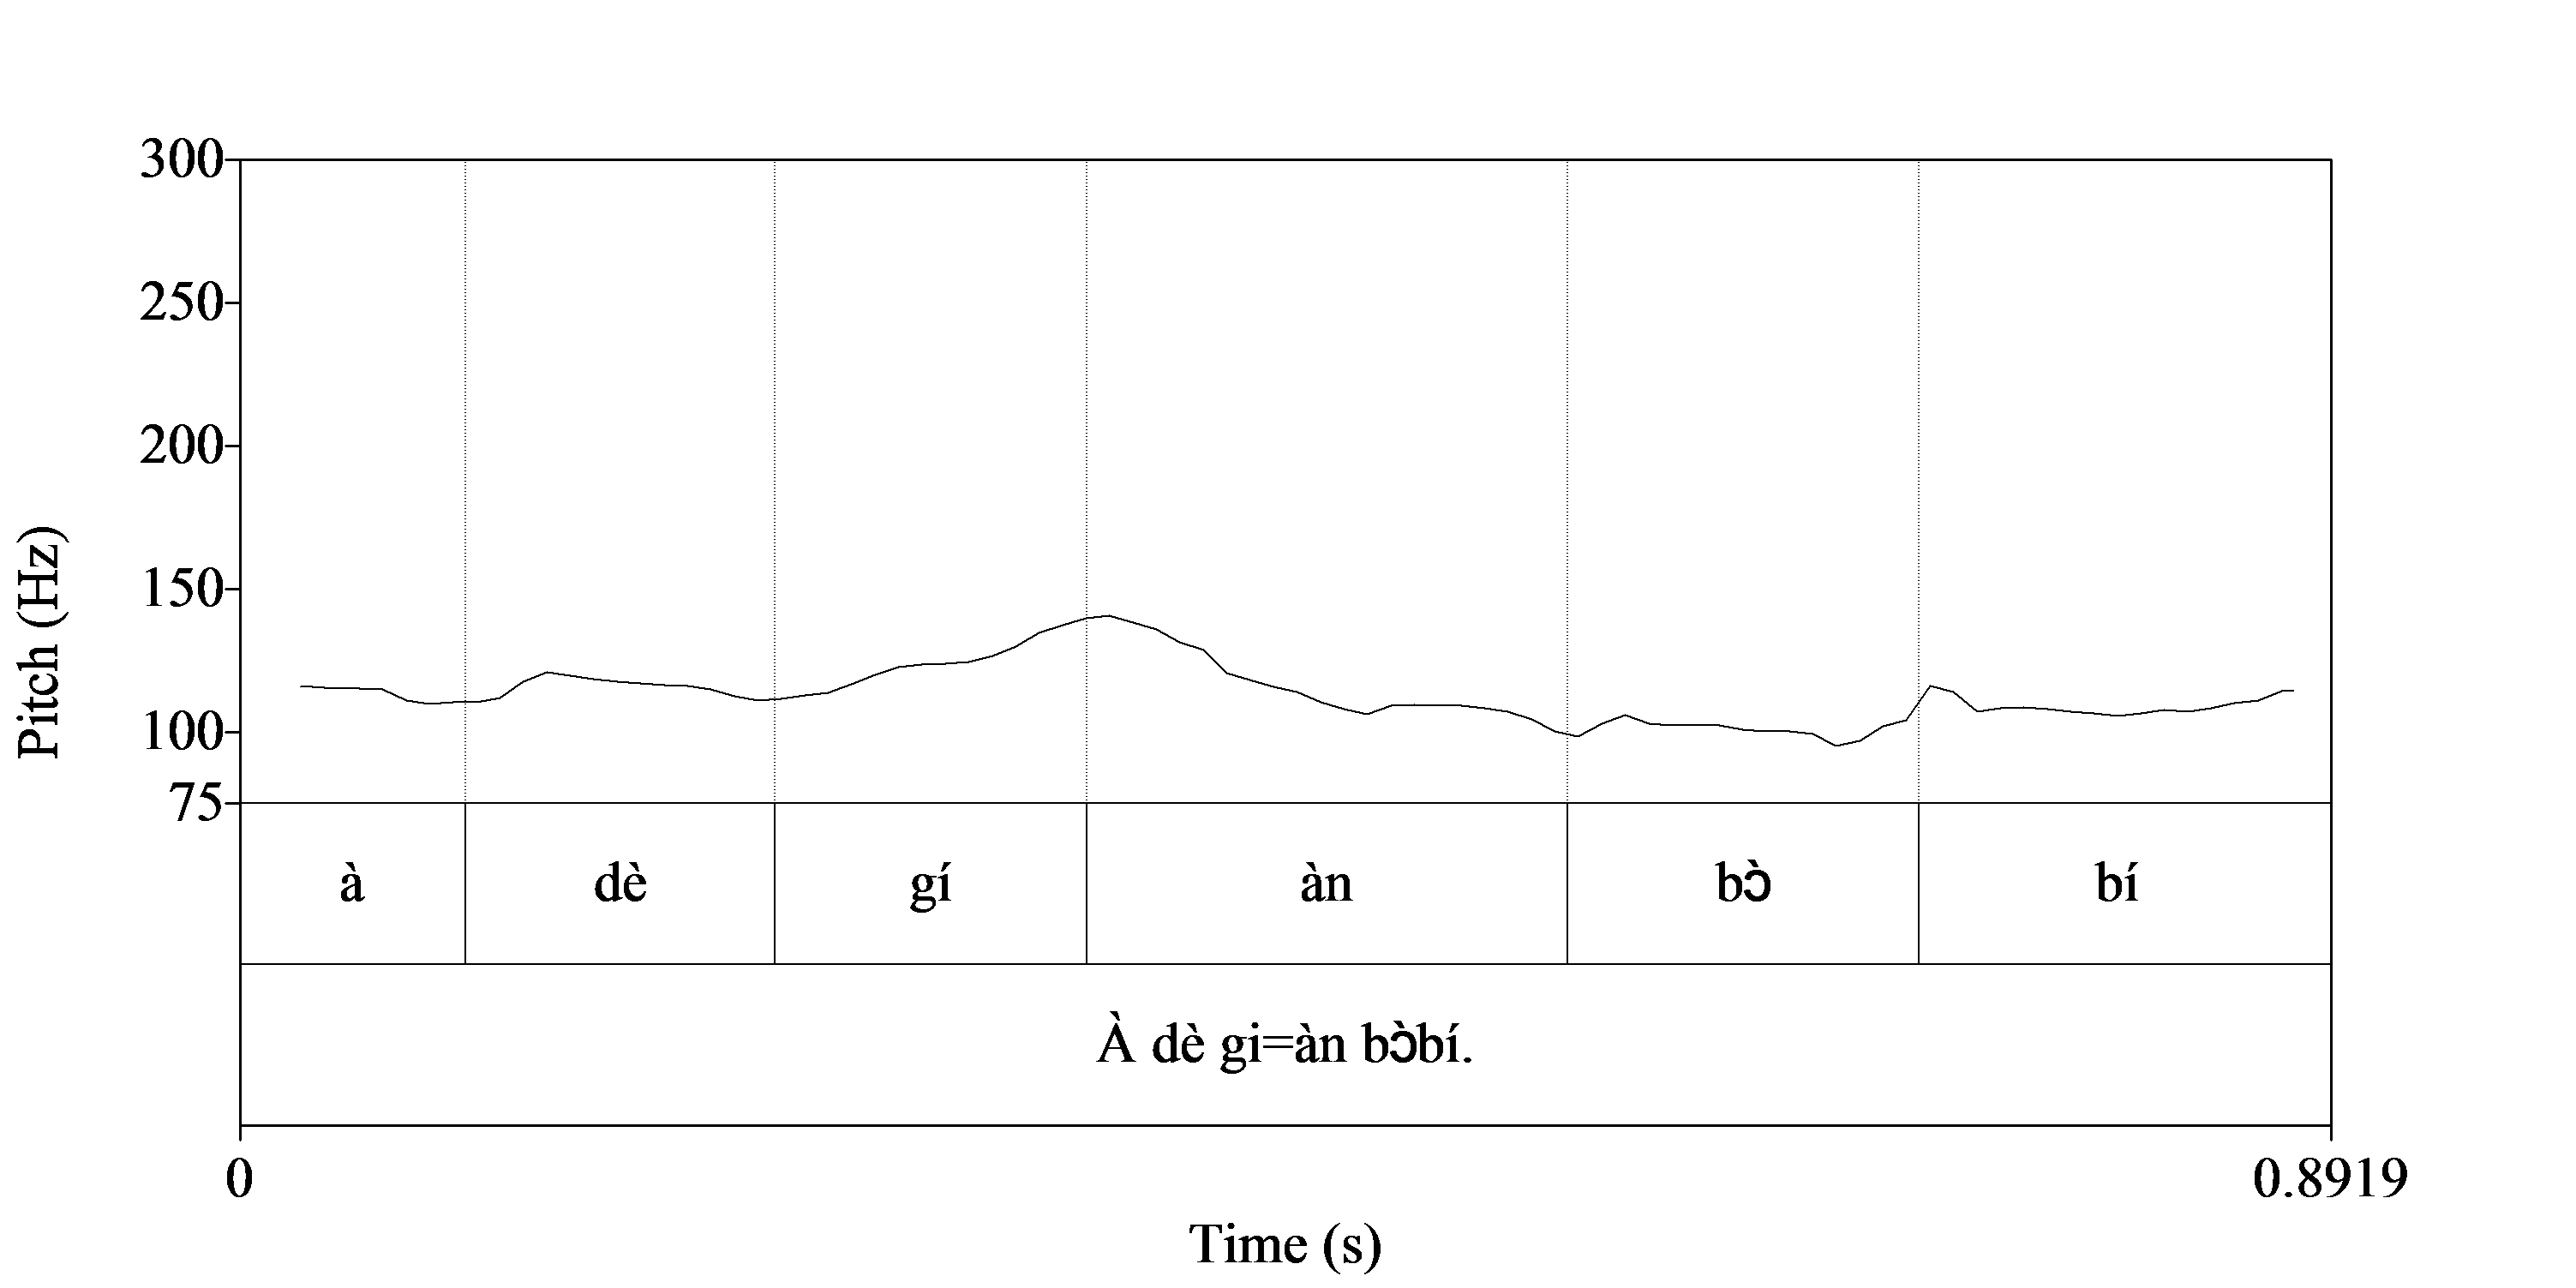
\includegraphics[height=.3\textheight]{figures/yakpomod-img30.png}
\end{figure}
 


\ea%81
    \label{ex:key:81}
    \gll   \MakeUppercase{A}   de    gí=an    bɔbí.\\
\textsc{l}    \textsc{l}    \textsc{h=l}      \textsc{l.}\textbf{\textsc{h}}\\


\textsc{1sg.sbj}  \textsc{ipfv}    give  =\textsc{3sg.obj}  breast\\

\glt ‘I’m breast-feeding her.’  

\z

Content questions\is{content questions} feature the same boundary tone as declaratives. Compare the utterance-final fall over the monosyllable in \figref{fig:key:3.29}:

\begin{figure}
\caption{L\% with content question}
\label{fig:key:3.29}
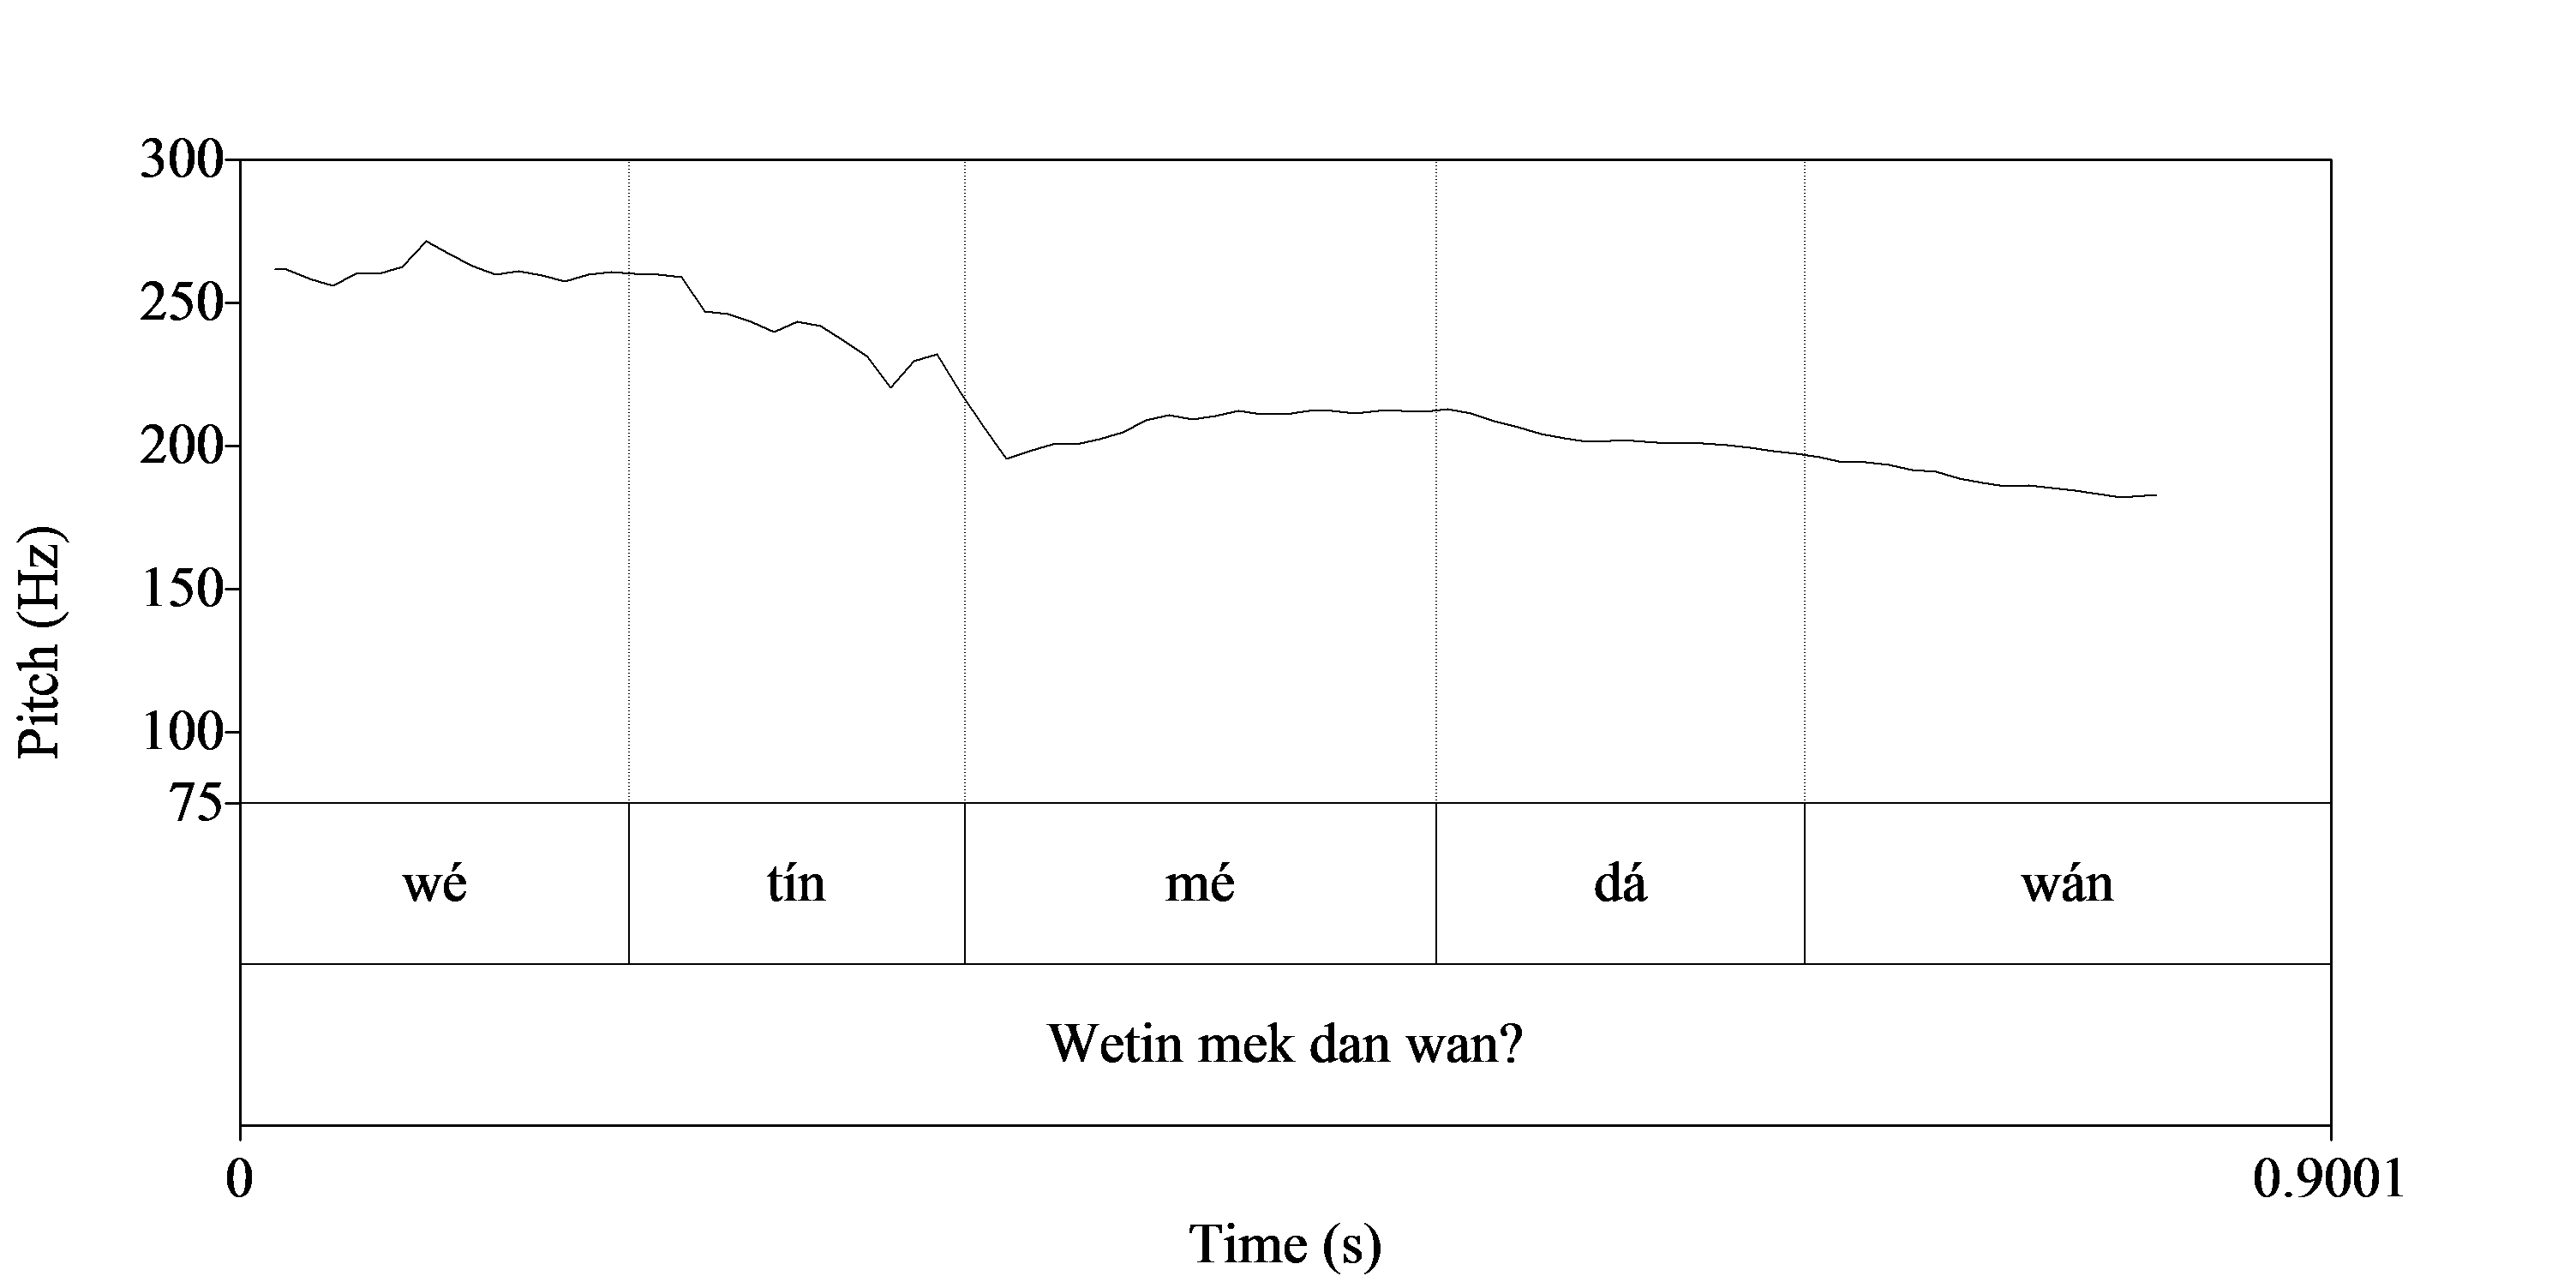
\includegraphics[height=.3\textheight]{figures/yakpomod-img31.png}
\end{figure}

  
 


\ea%82
    \label{ex:key:82}
    \gll   Wétin  mék    dán    \textbf{wán}?  \\
\textsc{h.l}    \textsc{h}    \textsc{h}    \textbf{\textsc{hl\%}}      \\
what  make  that    one\\
\glt ‘What causes this?’\is{declarative intonation}
\z

\subsection{Emphatic intonation}\label{sec:3.4.2}

Emphatic intonation expresses meanings like extra-emphasis, insistence, impatience or reproach. There are two ways of signalling emphasis\is{emphasis} at the sentence level in Pichi\is{emphatic stress}. One way involves the use of the emphatic LH\% boundary tone. A second way involves the use of pitch range expansion (cf. \sectref{sec:3.2.5}).


The emphatic LH\% is an additive contour tone. It succeeds the  lexical tone of the utterance-final syllable, which may therefore count up to three beats in length. Additionally, the last lexical H before the LH\% boundary contour tone is often pronounced with an extra-high tone due to emphasis. This peculiar combination of an extra-high lexical tone and a contour boundary tone creates a highly perceptible utterance-final tonal melody. 



Phonemically, an utterance-final L to which the emphatic LH\% boundary tone associates bears an LHH sequence of tones. Phonetically, the utterance-final syllable is realised as an LH contour. \figref{fig:key:3.30} depicts the utterance-final rise over the L-toned monosyllable \textit{=an} ‘\textsc{3sg.obj’}. 


\begin{figure}
\caption{Emphatic LH\% over L-final word}
\label{fig:key:3.30}
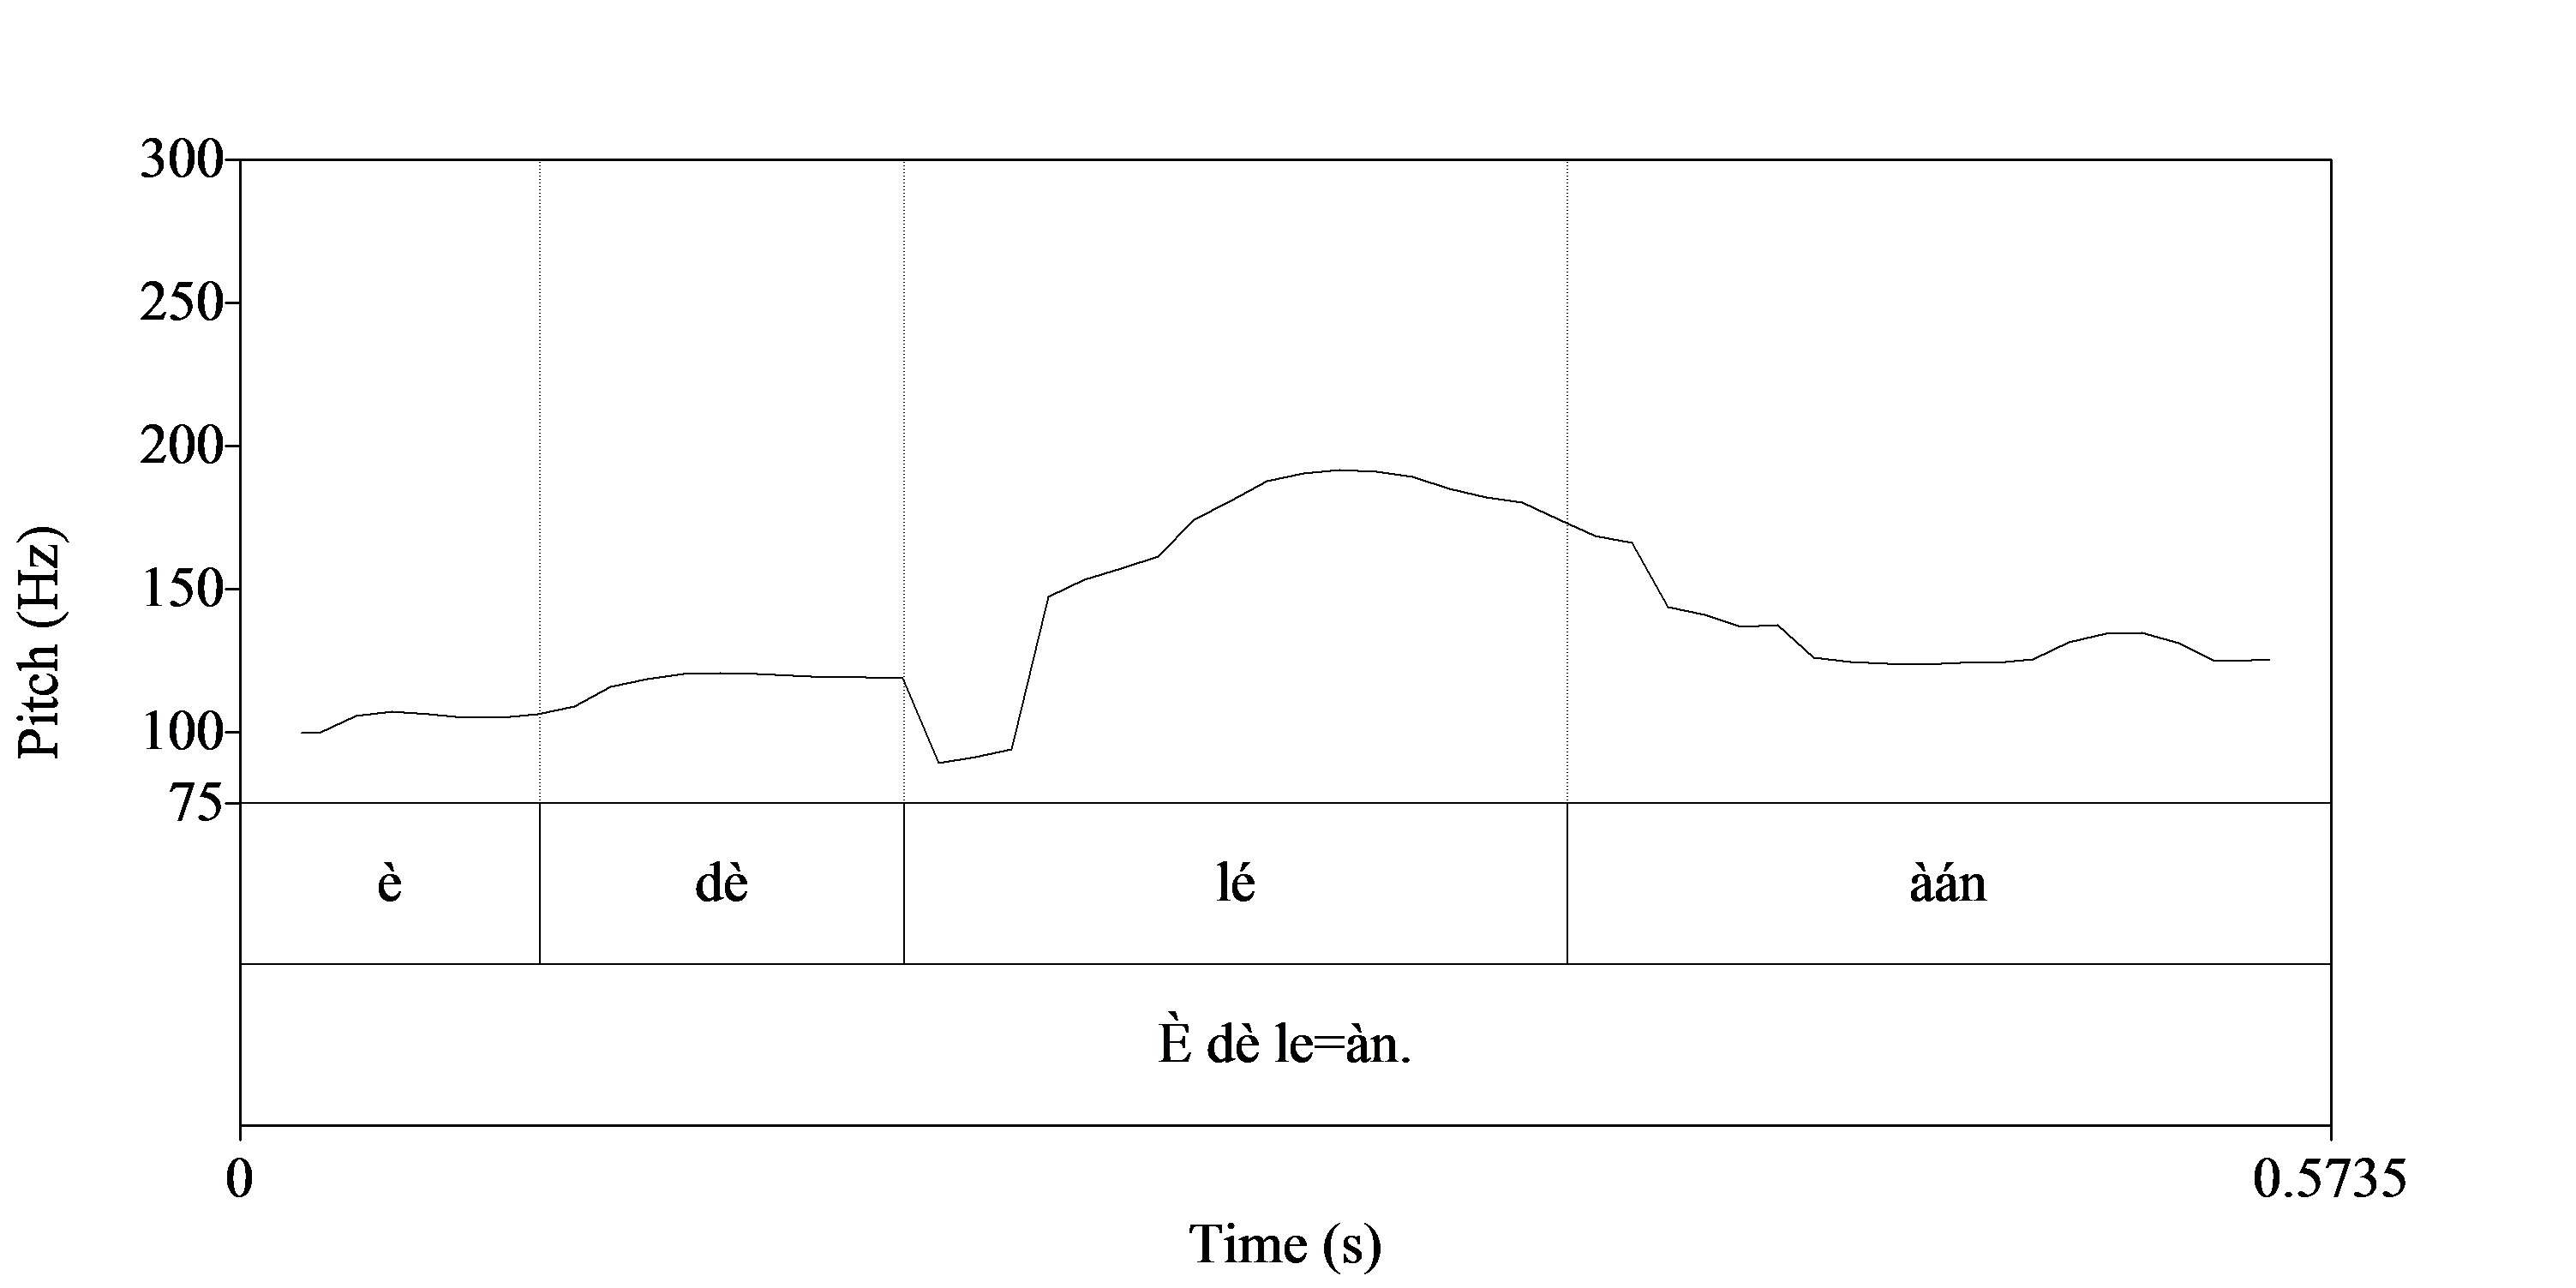
\includegraphics[height=.3\textheight]{figures/yakpomod-img32.png}
\end{figure}

  
 


\ea%83
    \label{ex:key:83}
    \gll   E    de  lé=an.\\
\textsc{l}    \textsc{l}  \textsc{h=}\textbf{\textsc{lh\%}}\\
\textsc{3sg.sbj}  \textsc{ipfv}    lay=\textsc{3sg.obj}\\
\glt ‘She is laying it (on the table).’
\z

When the emphatic boundary tone links with an utterance-final H-toned syllable the resulting contour features an initial rise, an intermediate fall, and a final rise. The utterance-final, extensively lengthened syllable thus bears an HLH contour. Compare the utterance-final H-toned monosyllables \textit{ín} ‘\textsc{3sg.indp}’ and \textit{gó} ‘go’ in the following two tables: 

% TODO: put in quadrant

\begin{figure}
\caption{Emphatic LH\% over H-final word}
\label{fig:key:3.31}
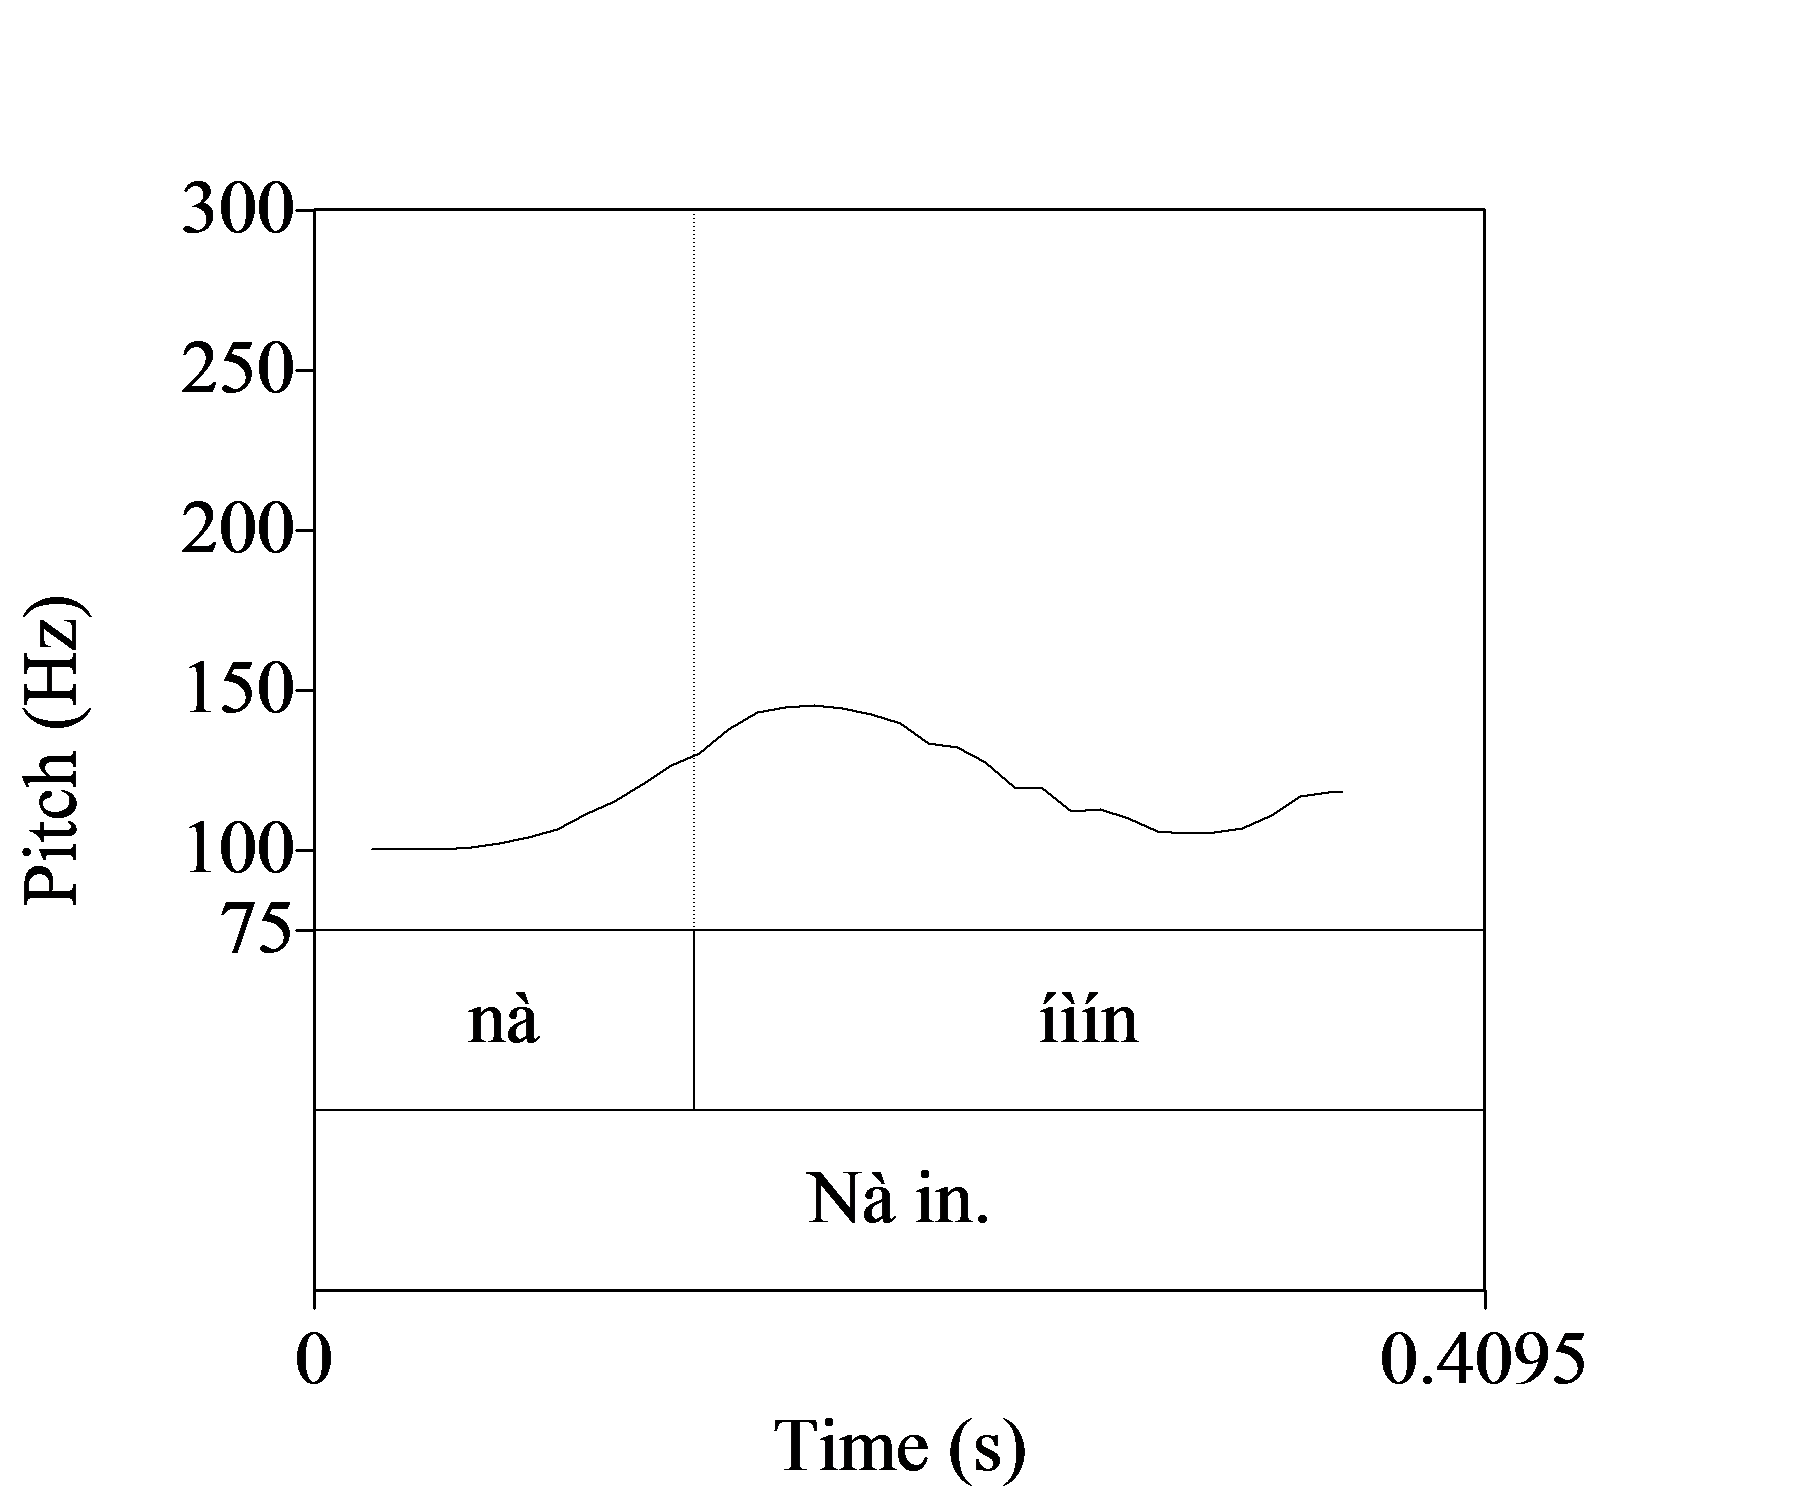
\includegraphics[height=.3\textheight]{figures/yakpomod-img33.png}
\end{figure}

\begin{figure}
\caption{Emphatic LH\% over H-final word}
\label{fig:key:3.32}
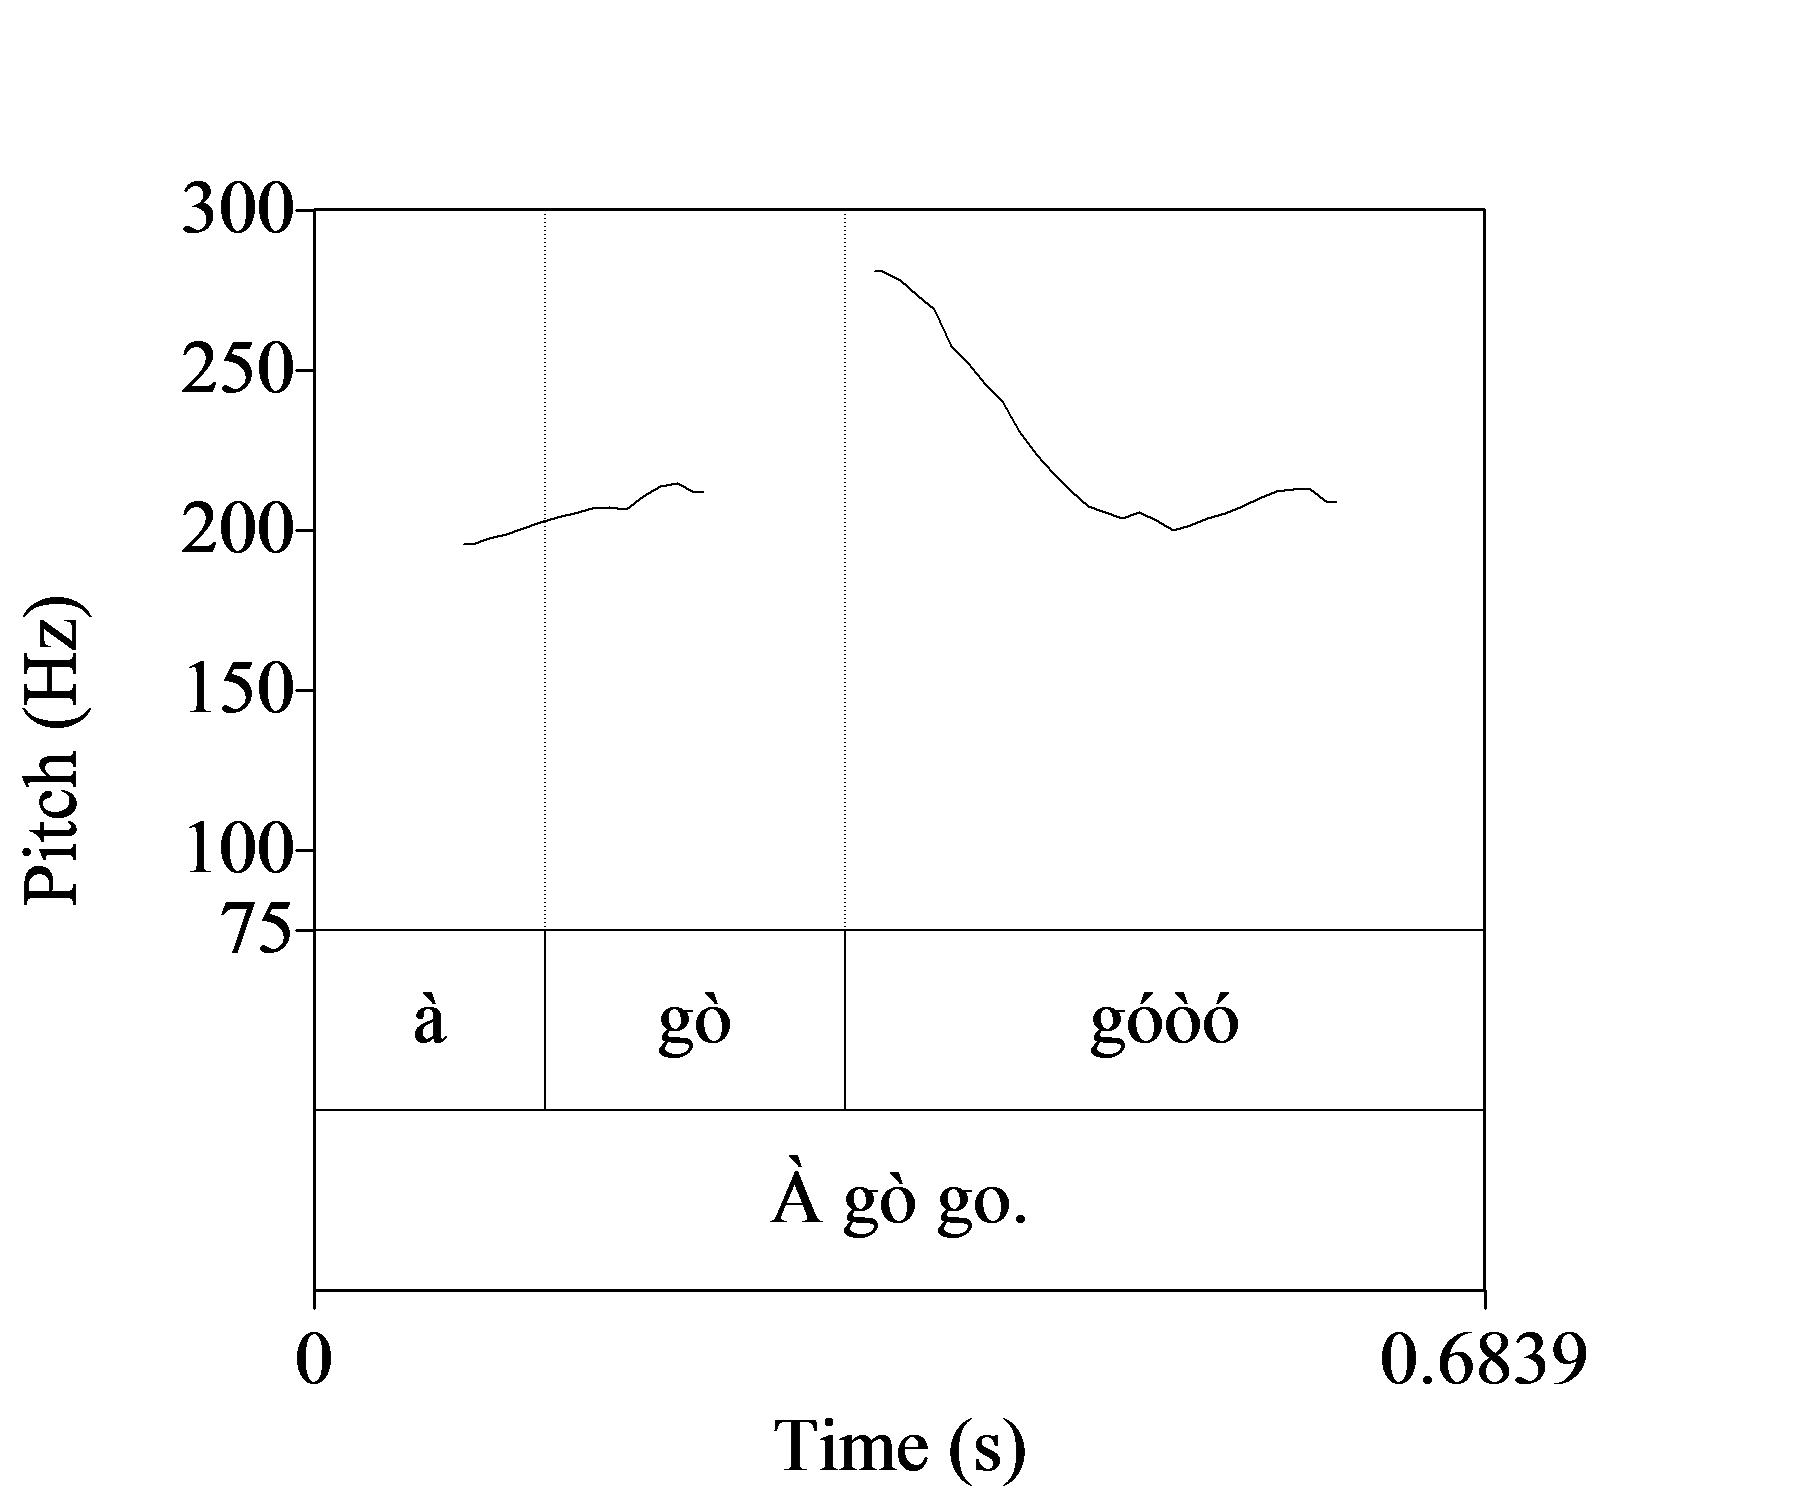
\includegraphics[height=.3\textheight]{figures/yakpomod-img34.png}
\end{figure}  

\ea\label{ex:key:84}
\glll Na  \textstylePichiexamplebold{ín}.''\\
\textsc{l}  \textbf{\textsc{h}}\textstylePichiexamplebold{\textsc{lh\%}}\\
\textsc{foc}  \textsc{3sg.indp}\\
\glt   ‘That’s it [you should know that].’
\z
\ea\label{ex:key:85}
\glll    A    go  \textbf{gó}.  \\
\textsc{l}    \textsc{l}  \textbf{\textsc{h}}\textstylePichiexamplebold{\textsc{lh\%}}\\
\textsc{1sg.sbj}  \textsc{pot}  go\\
\glt   ‘I’ll go [you don’t need to remind me to].’ 
\z

An utterance-final, H-toned syllable of a polysyllabic word also bears this contour. Compare \textit{bɔbí} ‘breast’ and \textit{chukchúk} ‘thorn’ in the following tables. The two words were pronounced with emphatic intonation during vocabulary elicitation because the speaker expected me to be familiar with them: 

\begin{figure}
\caption{H\% over vowel-final L.H word}
\label{fig:key:3.33}
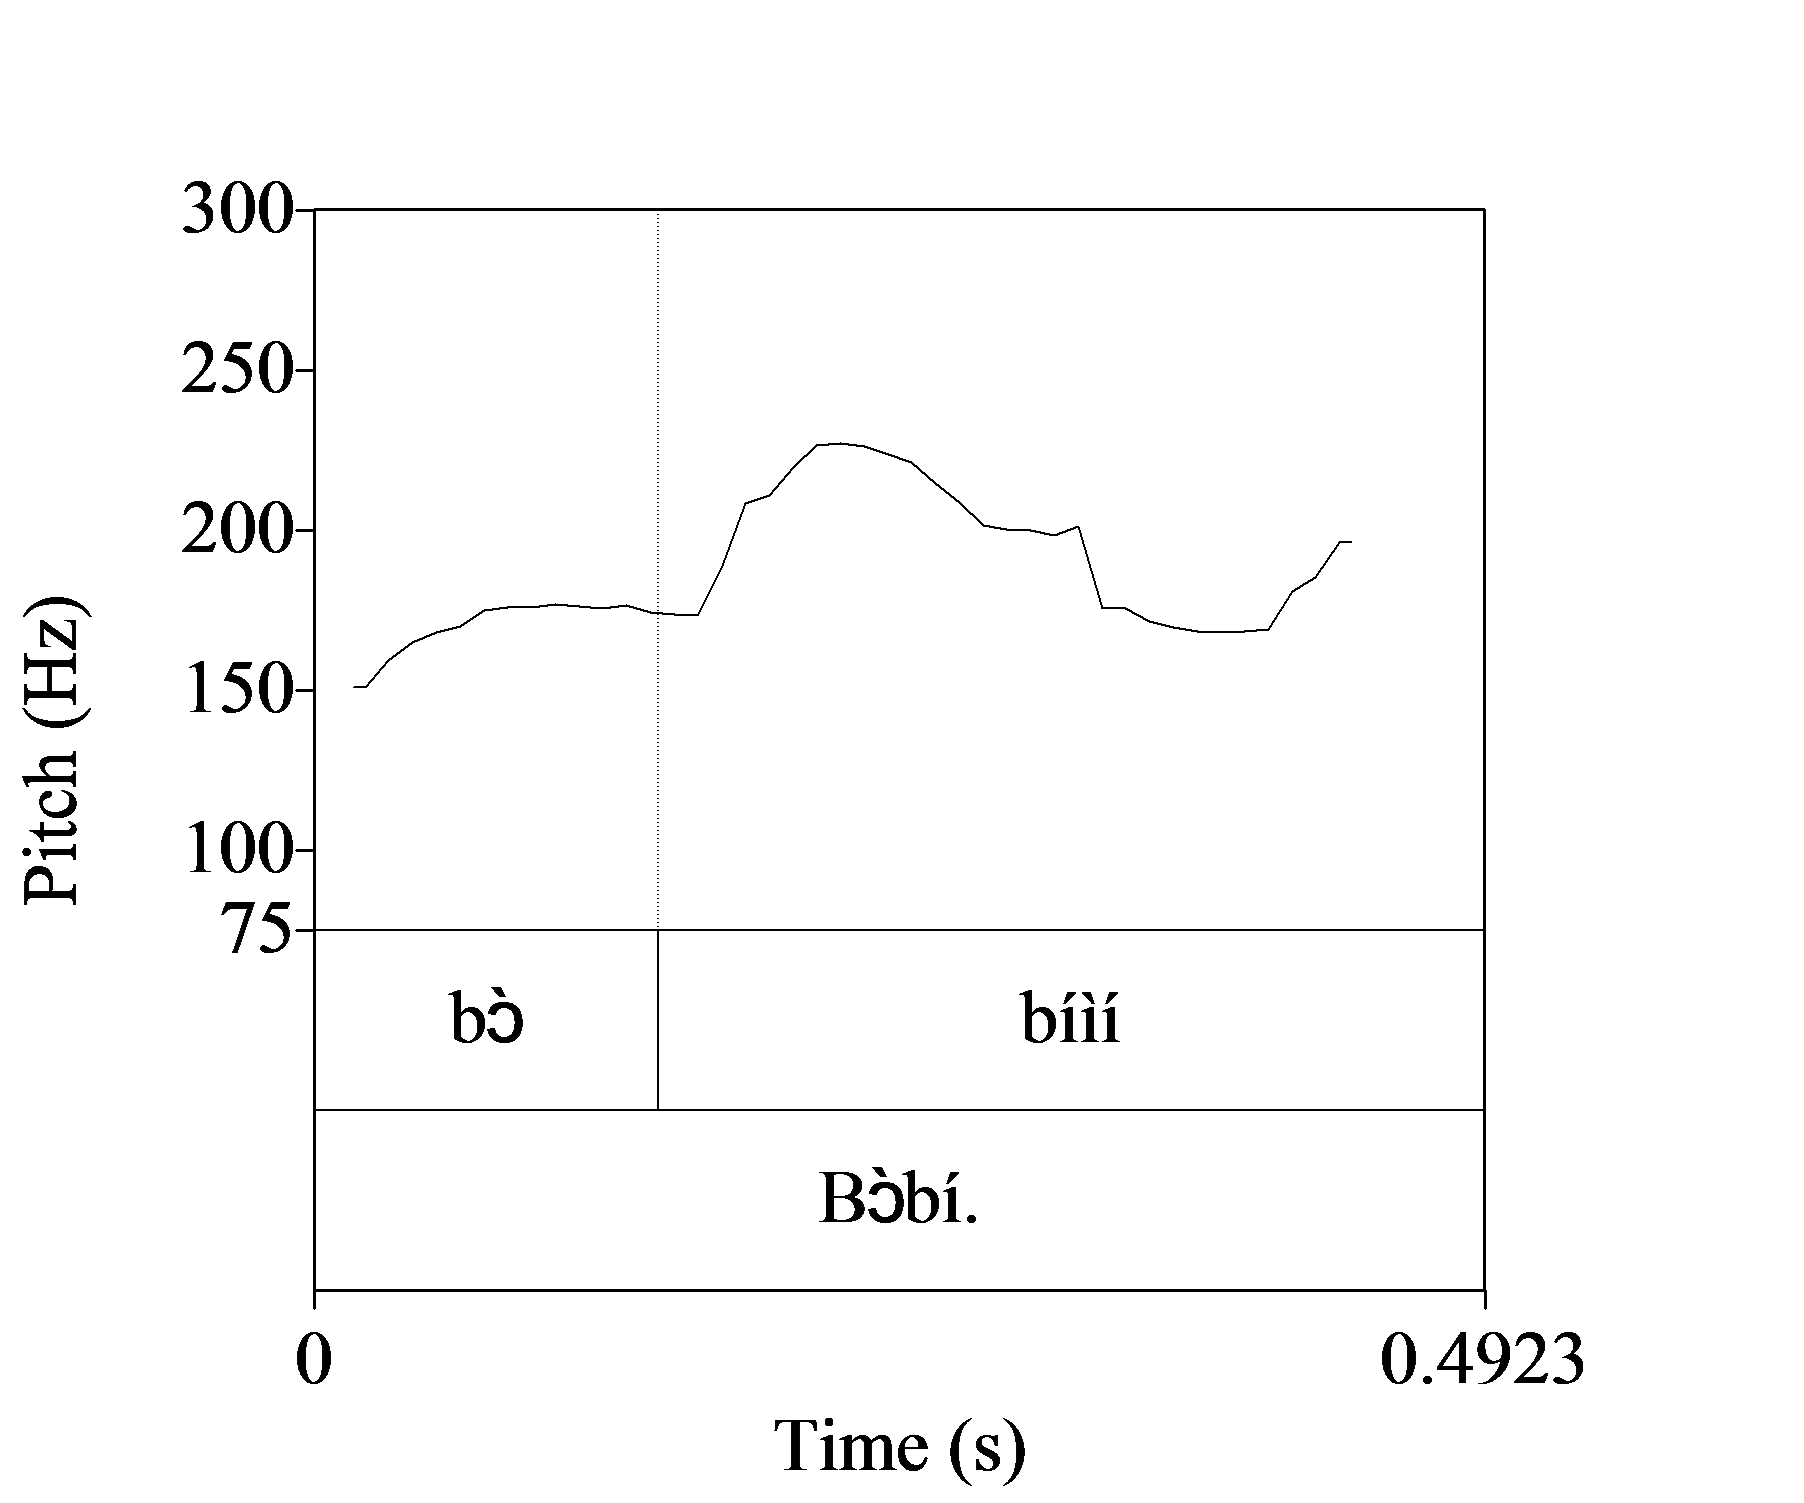
\includegraphics[height=.3\textheight]{figures/yakpomod-img35.png}
\end{figure}


\begin{figure}
\caption{H\% over obstruent-final L.H word}
\label{fig:key:3.34}
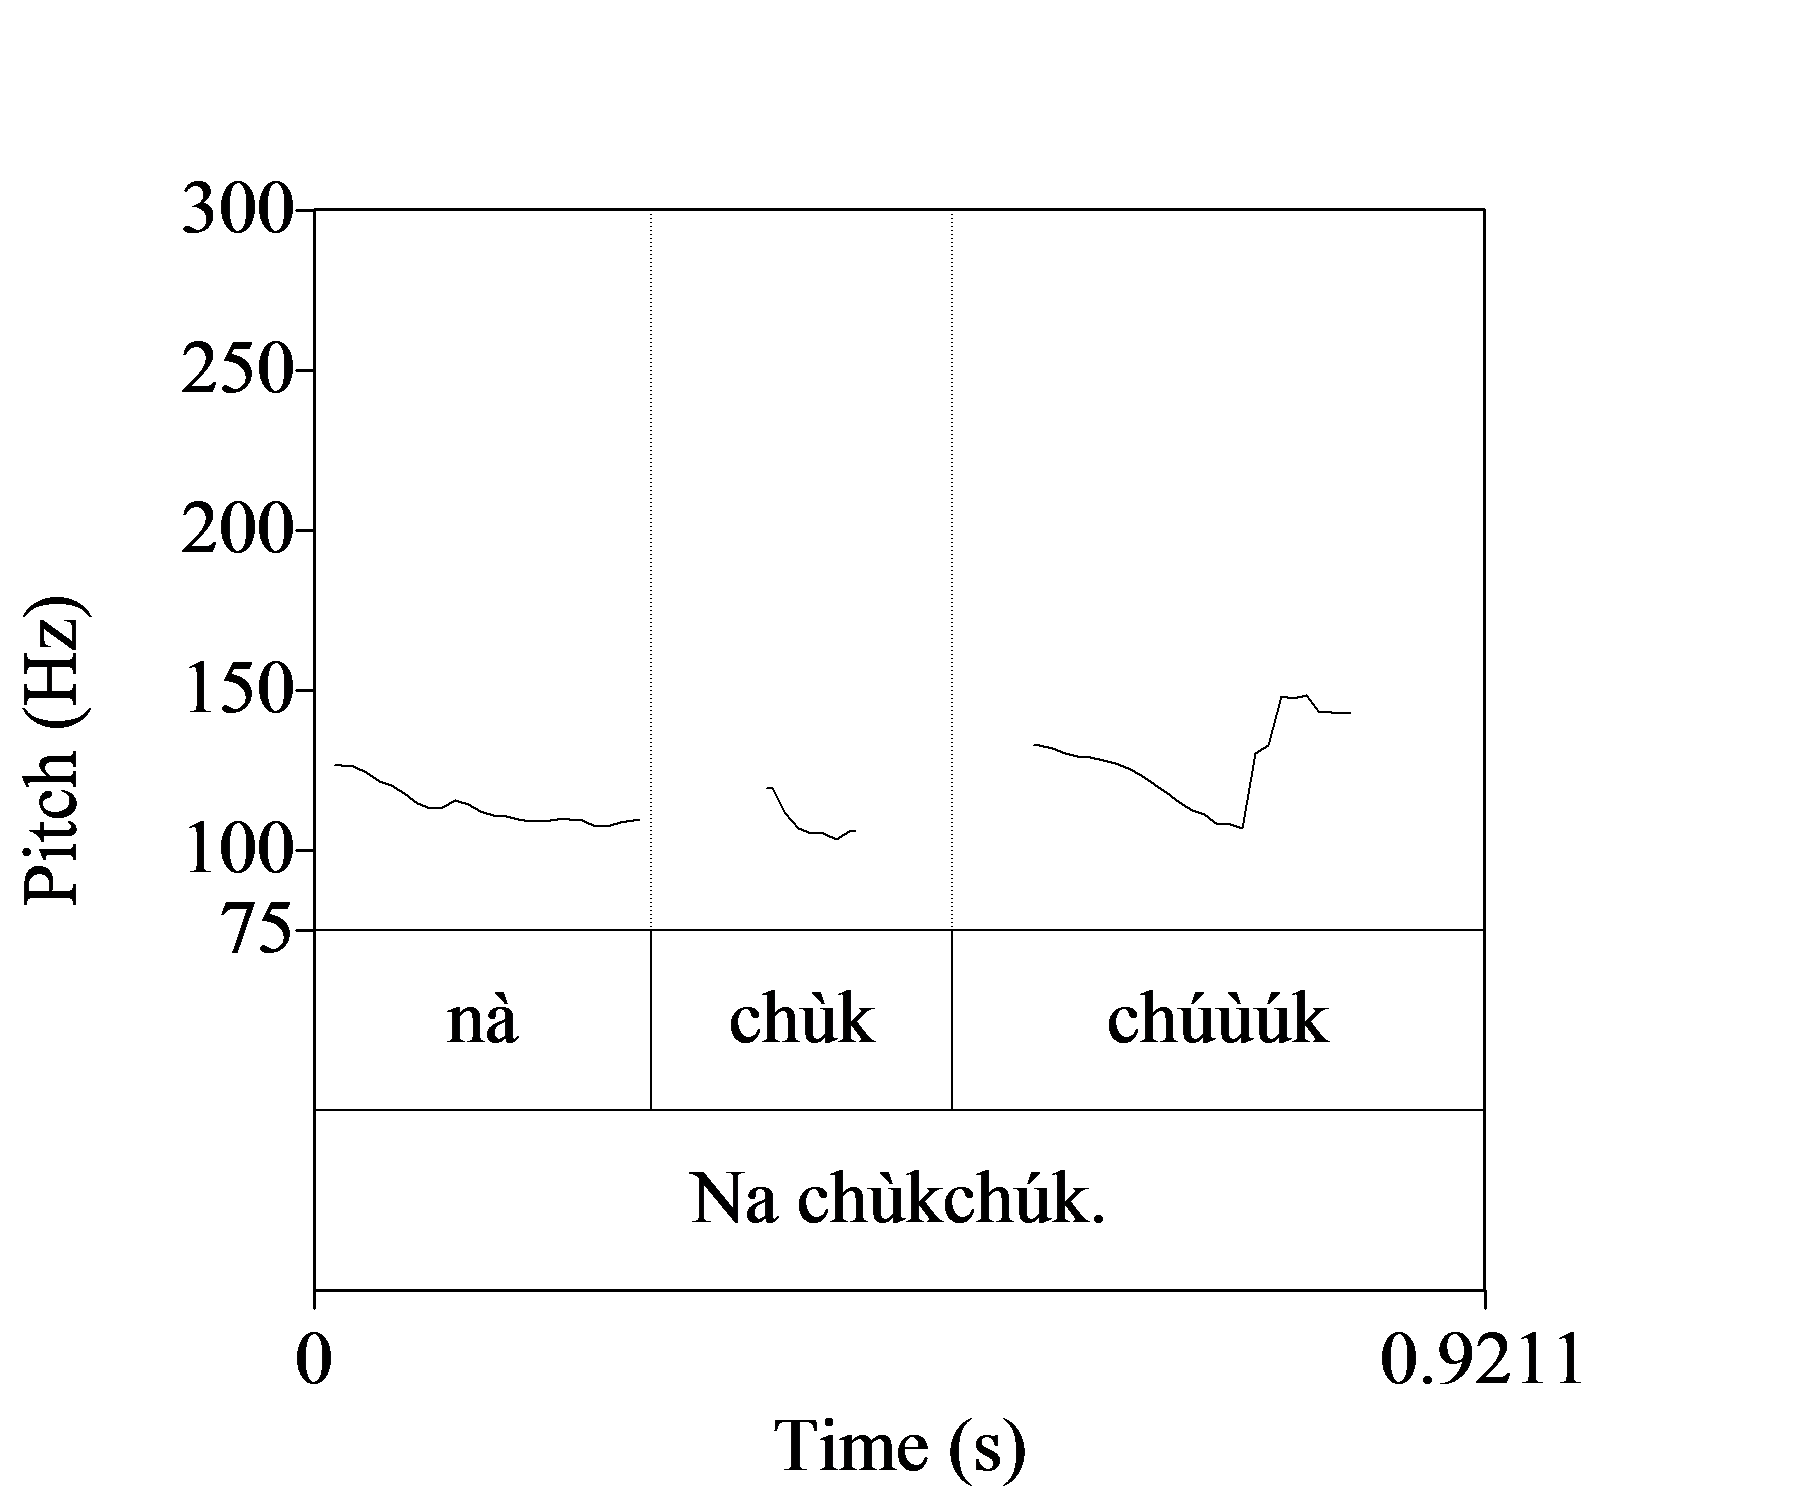
\includegraphics[height=.3\textheight]{figures/yakpomod-img36.png}
\end{figure}

\ea%86
    \label{ex:key:86}
    \glll   Bɔbí.\\
\textsc{l.}\textbf{\textsc{h}}\textstylePichiexamplebold{\textsc{lh\%}}\\
breast\\
\glt ‘Breast [that’s self-evident!].’ 
\z

\ea
\label{ex:key:87}
\glll \textstylePichiexamplenumberZchnZchn{Na  chukchúk}\\
\textsc{l}  \textsc{l.}\textbf{\textsc{hlh\%}}\\
\textsc{foc}  thorn\\
\glt ‘It’s a thorn [that’s self-evident].’\is{emphatic intonation}
\z
The LH\% boundary contour tone is a loan\is{loan intonation} from (Equatoguinean and, ultimately, Iberian) Spanish together with the meanings associated with it. The LH\% contour boundary tone is also employed for list intonation \is{list intonation}(cf. \sectref{sec:3.4.3}). The following table presents the pitch trace of an utterance in Equatoguinean Spanish.


Compare the contour over the utterance-final L-toned syllable with that borne by the utterance-final L-toned syllable in \figref{fig:key:3.30} further below. Also compare the emphatic contour over the phonologically independent \textit{sí} ‘yes’ with that of the high-toned \textit{ín} ‘\textsc{3sg.indp}’ in \figref{fig:key:3.31}:


\begin{figure}
\caption{Emphatic intonation in peninsular Spanish}
\label{fig:key:3.35}
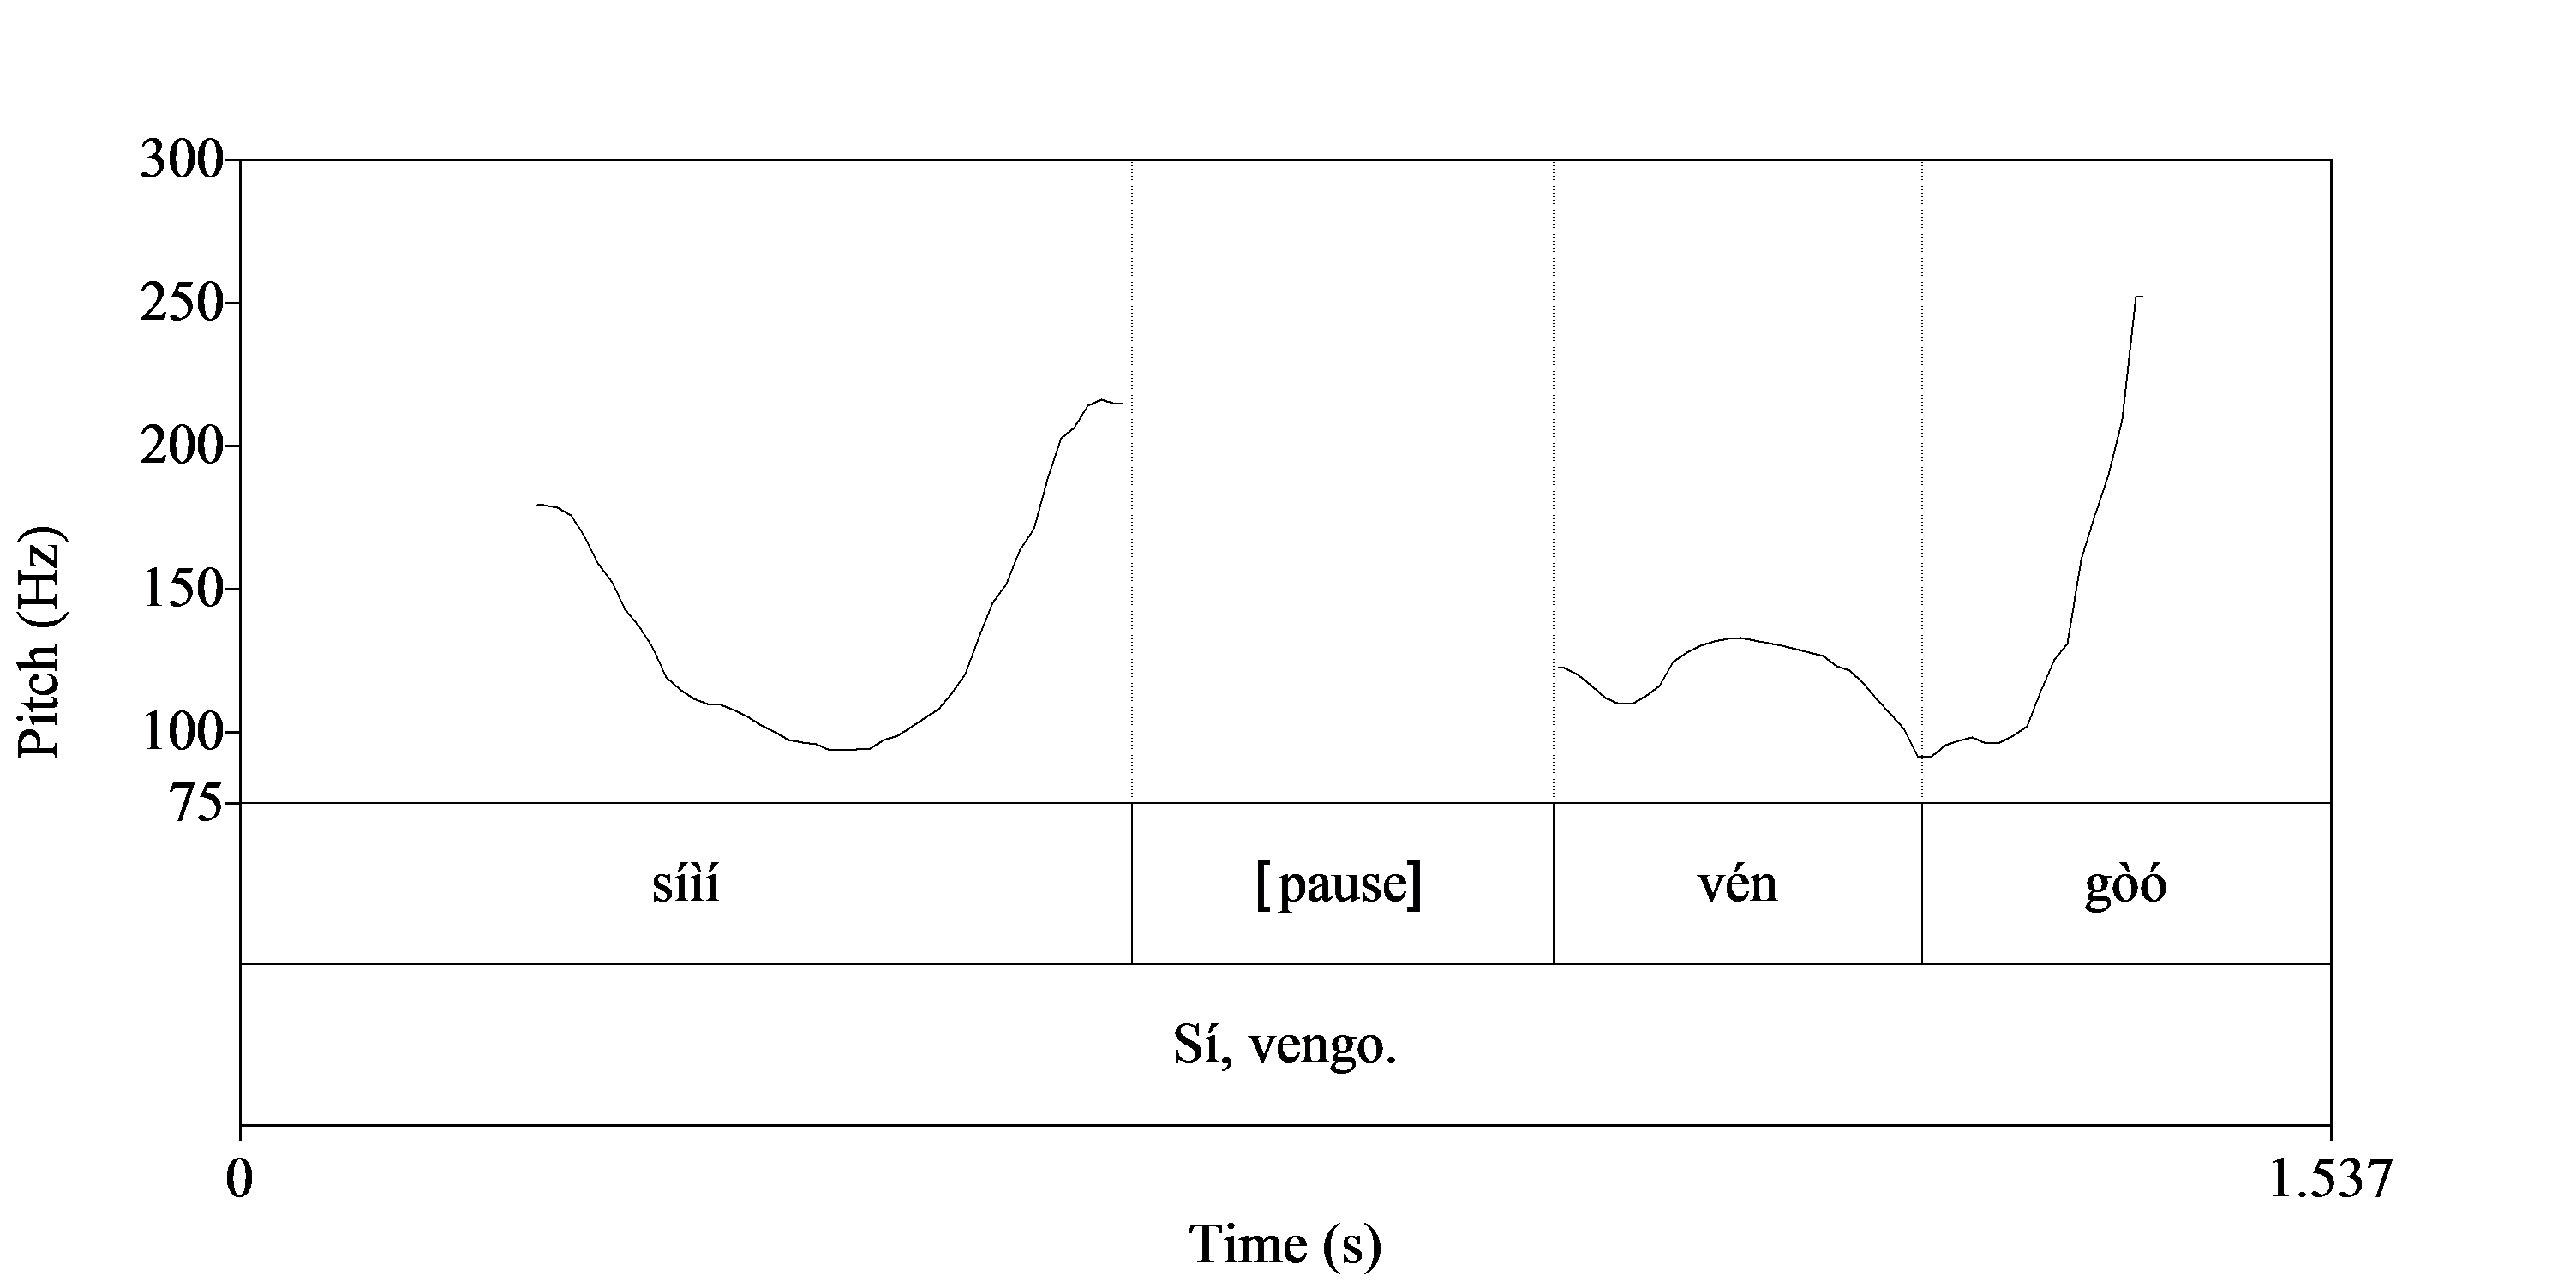
\includegraphics[height=.3\textheight]{figures/yakpomod-img37.png}
\end{figure}
 


\ea%88
    \label{ex:key:88}
    \glll   Sí    vengo.\\
\textsc{h}\textstylePichiexamplebold{\textsc{lh\%}}  \textsc{h.}\textstylePichiexamplebold{\textsc{lh\%}}\\
yes    I.come\\
\glt ‘Yes [you should know that!], I’ll come.’
\z

\subsection{List intonation}\label{sec:3.4.3}

The additive LH\% boundary tone employed for emphatic intonation is also used for list intonation. As in emphatic declaratives, LH\% associates with the final syllable and creates an LH contour over an utterance-final L-toned syllable and an HLH contour over an utterance-final H-toned syllable. The same intonation contour is once more found in Equatoguinean (and Iberian) Spanish with a similar range of meanings.


The following three pitch traces form part of a list. Take note of the LH contour over the L-toned dependent pronoun \textit{dɛn} ‘\textsc{3pl}’ before the short pause, as well as the LH contour borne by the L-toned final syllable of \textit{manicura} ‘manicure’ in \figref{fig:key:3.36} and \textit{chía} ‘chair’ in \figref{fig:key:3.36}. Compare this with the declarative L\% over \textit{dé} ‘there’, the closing sentence of the list in \figref{fig:key:3.38}: 


\begin{figure}
\caption{List intonation}
\label{fig:key:3.36}
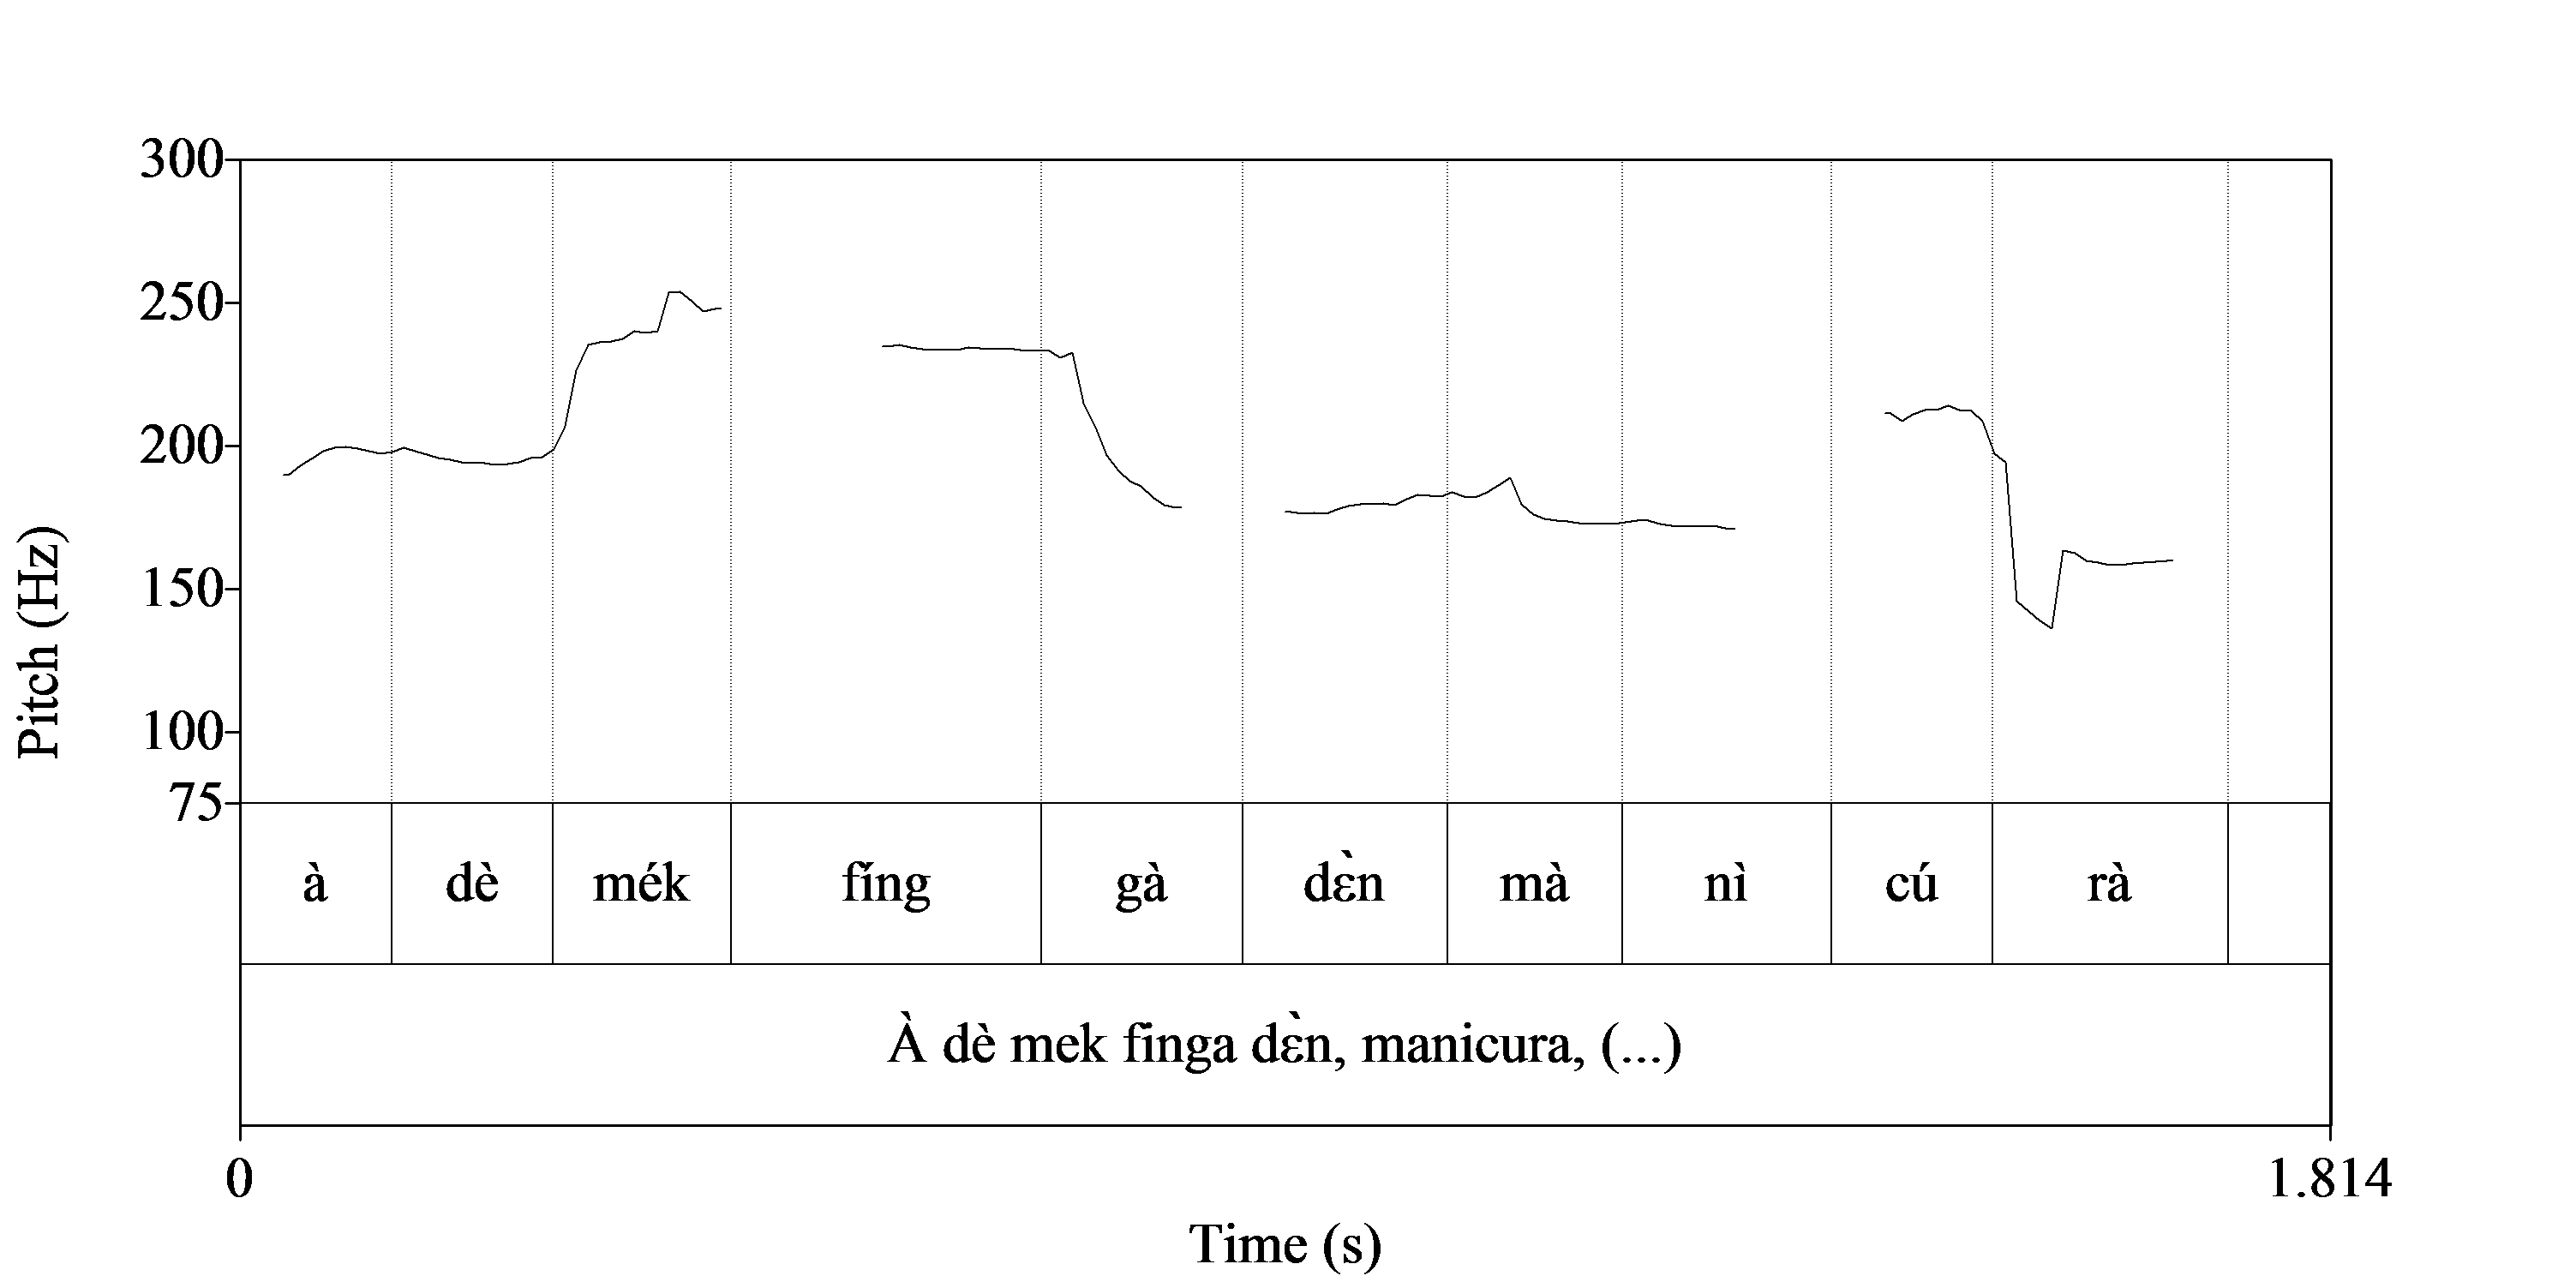
\includegraphics[height=.3\textheight]{figures/yakpomod-img38.png}
\end{figure}

  
 


\ea%89
    \label{ex:key:89}
    \glll   A    de  mék    fínga  \textstylePichiexamplebold{dɛn},    manicu\textbf{ra},  (...)\\
\textsc{l}    \textsc{l}  \textsc{h}    \textsc{h.l}    \textbf{\textsc{lh\%}}    \textsc{l.l.}\textbf{\textsc{h.lh\%}}\\
\textsc{1sg.sbj}  \textsc{ipfv}  make  finger  \textsc{pl}    manicure\\
\glt ‘I was making fingers, manicure (...)’
\z

\begin{figure}
\caption{List intonation}
\label{fig:key:3.37}
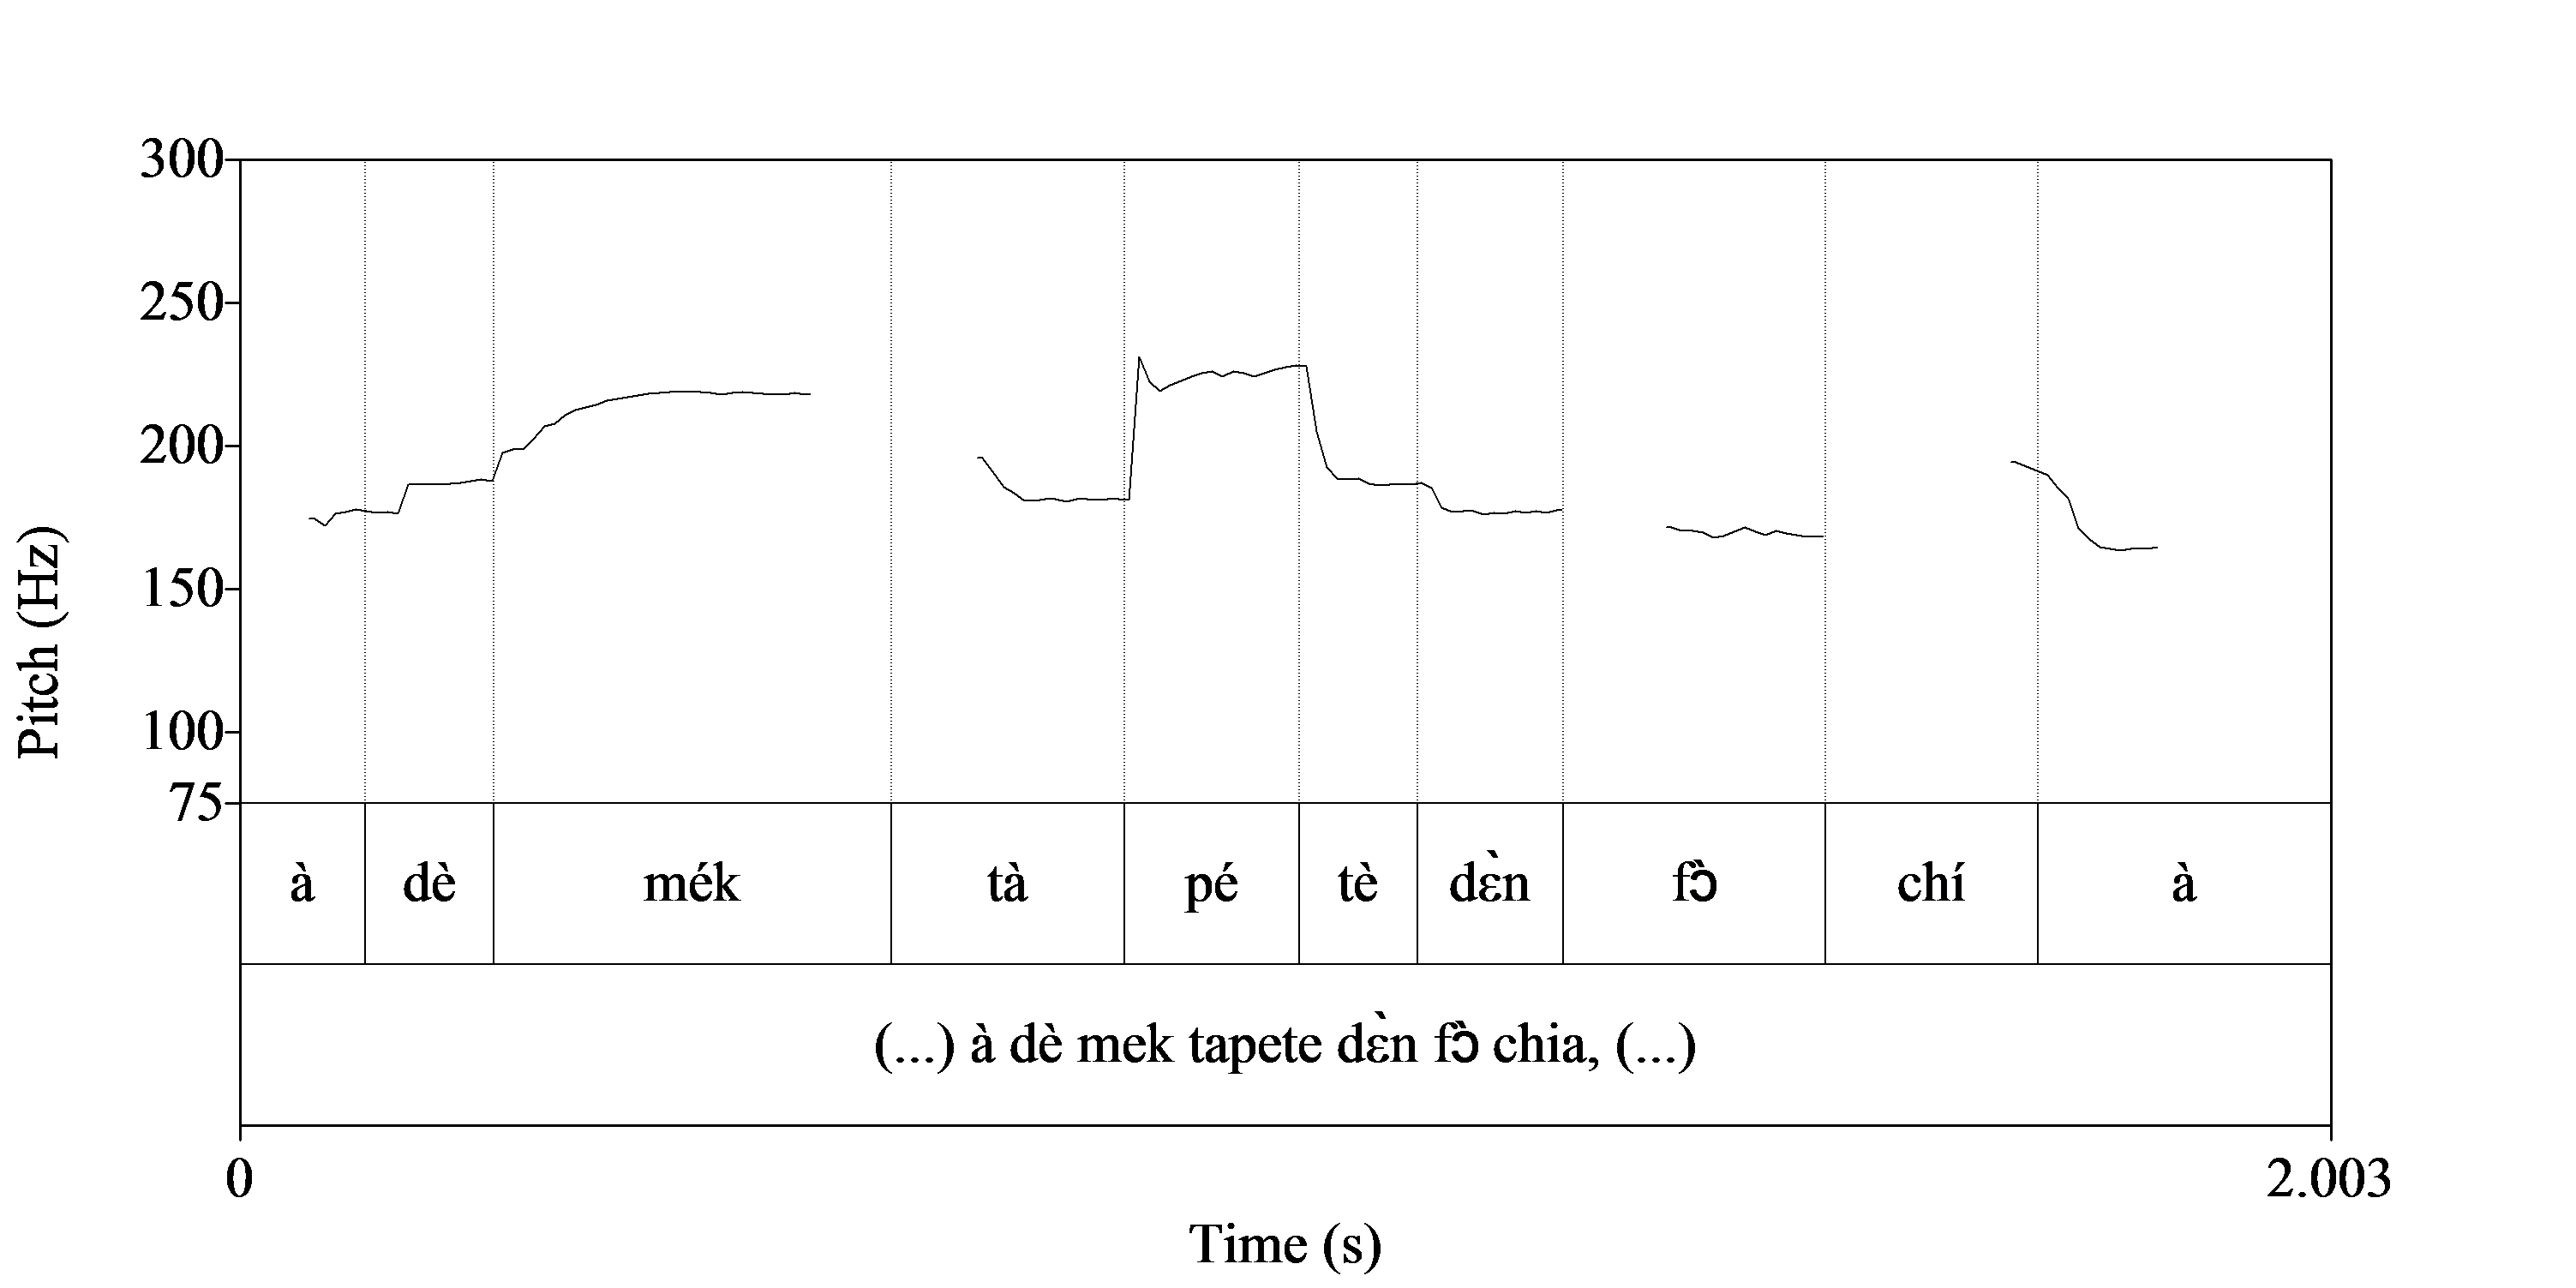
\includegraphics[height=.3\textheight]{figures/yakpomod-img39.png}
\end{figure}
 


\ea%90
    \label{ex:key:90}
    \glll   (...)  a    de  mék    tapete  dɛn  fɔ  chía, (…)\\
{}  \textsc{l}    \textsc{l}  \textsc{h}    \textsc{l.h.l}    \textsc{l}  \textsc{l}  \textsc{h.}\textbf{\textsc{lh\%}}\\
{}  \textsc{1sg.sbj}  \textsc{ipfv}  make  cloth  \textsc{pl}  \textsc{prep}  chair\\
\glt ‘(...)  I was making chair-drapings, (...)’
\z

\begin{figure}
\caption{Declarative L\% over final item in list\is{declarative intonation}}
\label{fig:key:3.38}
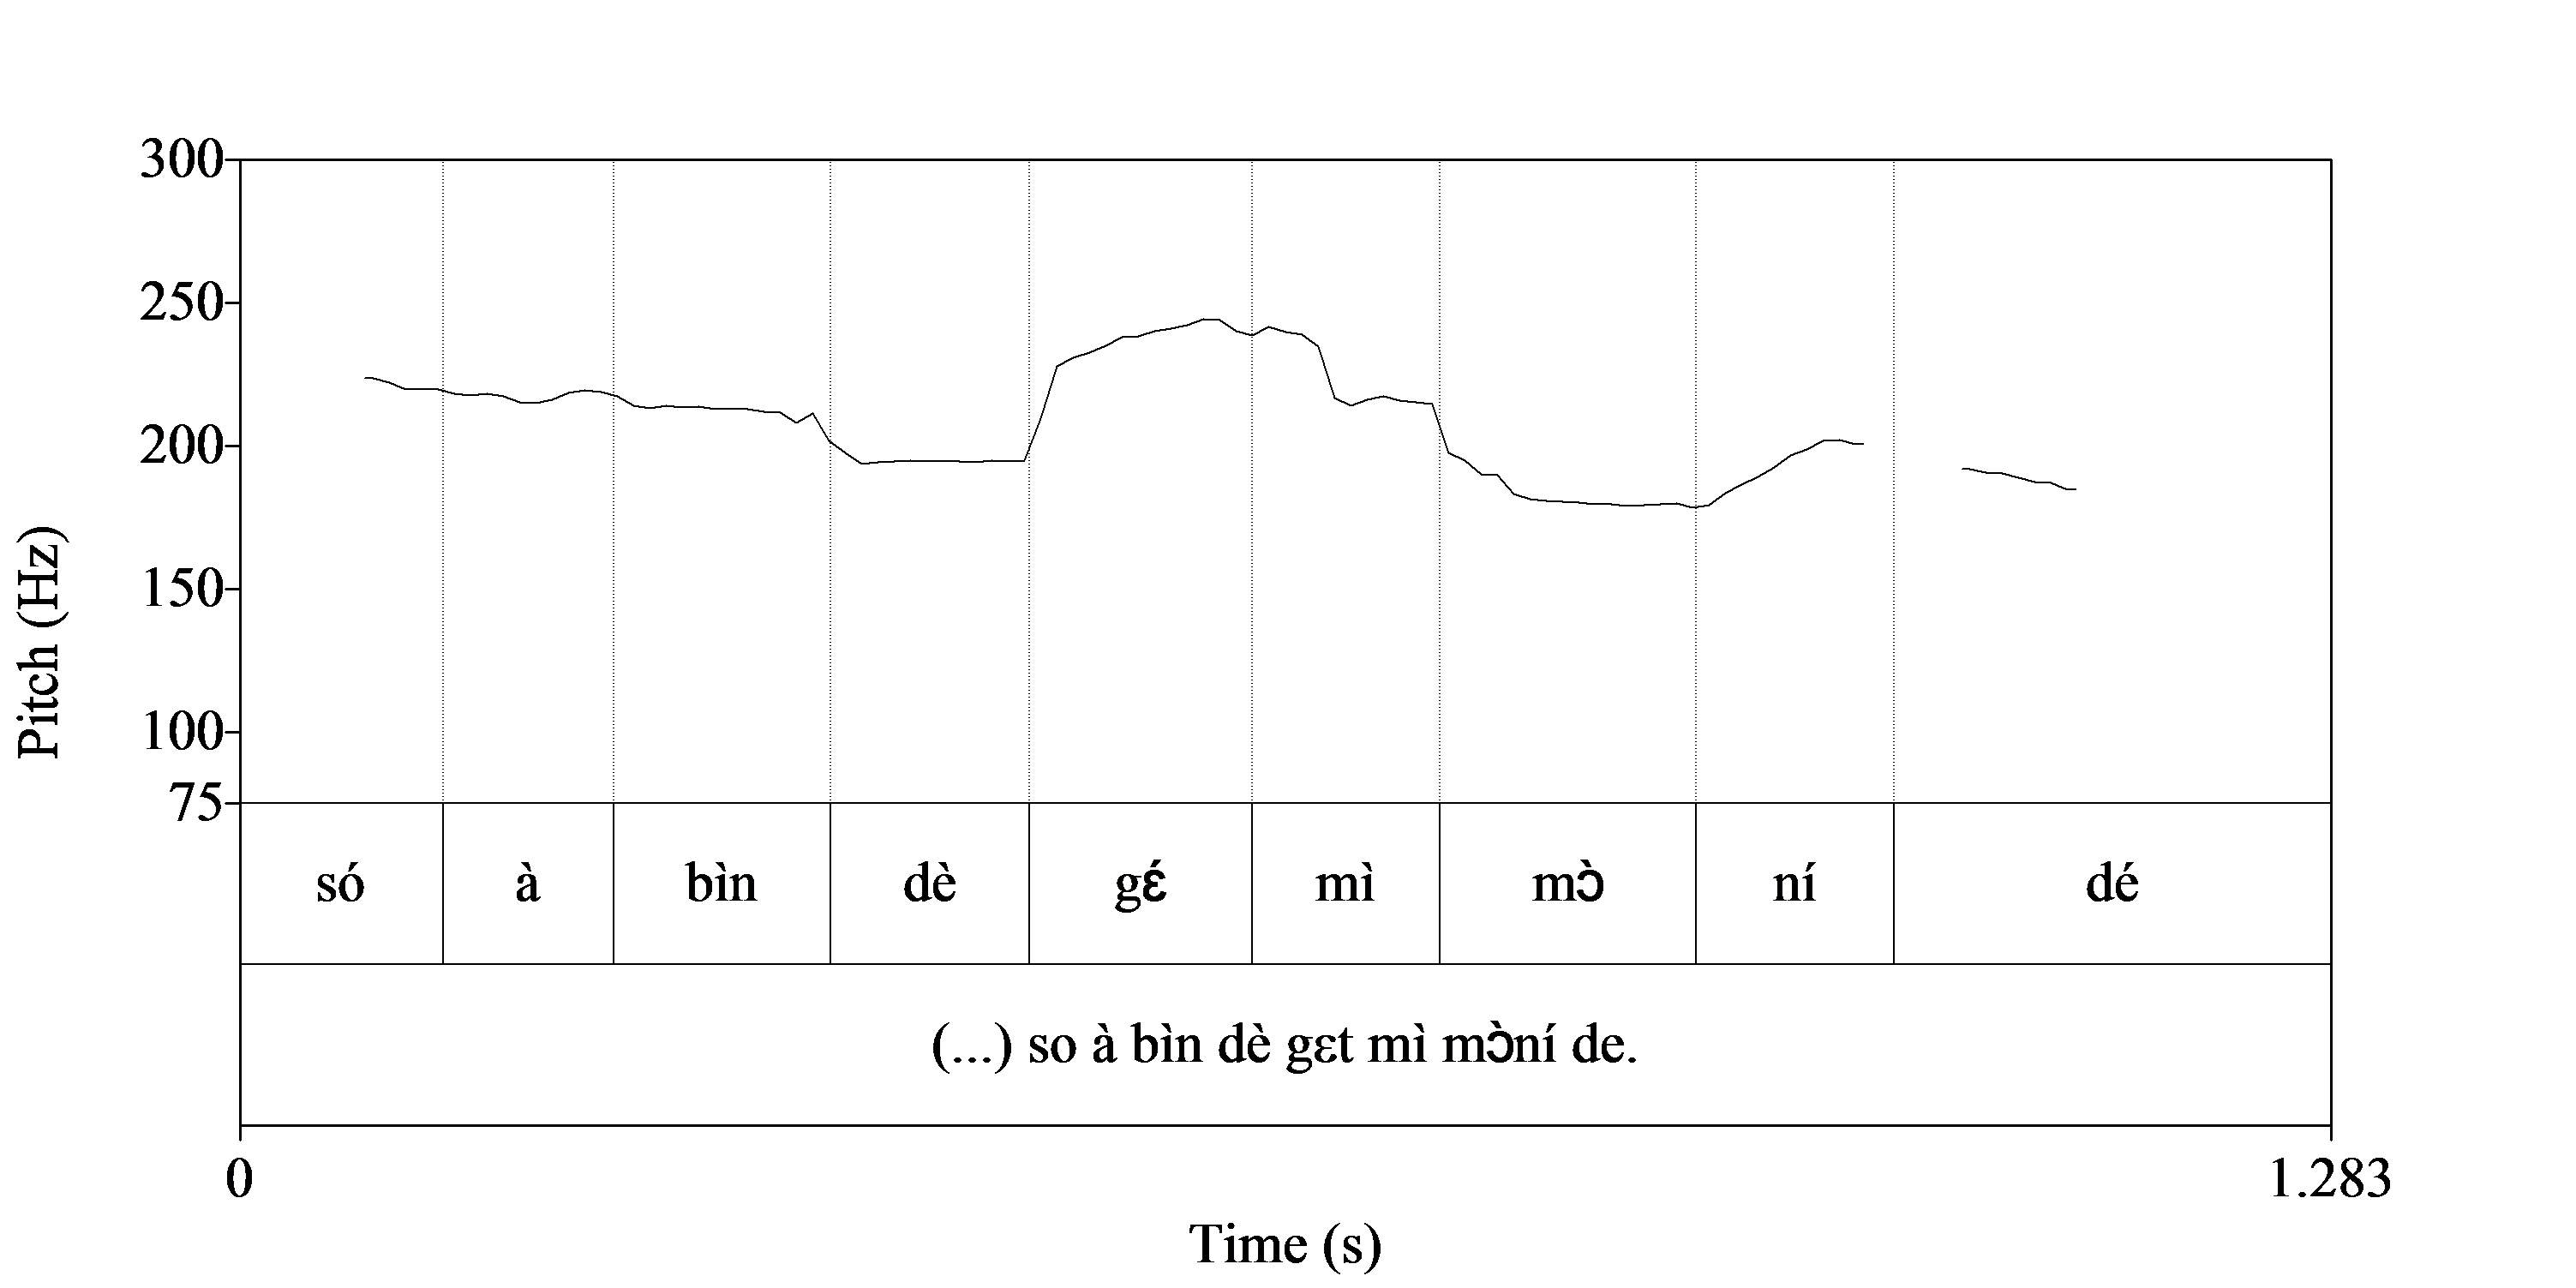
\includegraphics[height=.3\textheight]{figures/yakpomod-img40.png}
\end{figure}

  
 


\ea%91
    \label{ex:key:91}
    \glll   (...)  só  a    bin  dé  gɛ́t  mí    mɔní  dé.\\
  \textsc{h}  \textsc{l}    \textsc{l}  \textsc{l}  \textsc{h}  \textsc{l}    \textsc{l.h}    \textsc{h}\textbf{\textsc{l\%}}\\
  so  \textsc{1sg.sbj}  \textsc{pst}  \textsc{ipfv}  get  \textsc{1sg.poss}  money  there\\
\glt ‘(...) so I was getting my money there.’\is{list intonation}
\z


\subsection{Continuative intonation}\label{sec:3.4.4}

The absence of a boundary tone, usually before a prosodic break (a brief but audible pause), signals continuative intonation. With continuative intonation, the lexical tone of the relevant syllable simply maintains its pitch and is therefore pronounced with the same pitch as it would in utterance-medial position. Continuative intonation functions as a floor-holding device, a juncture marker on the right edge of utterances in order to prepare the ground for following material. Continuative intonation therefore plays an important role in signalling topic and focus next to the particles employed for this purpose (cf. \sectref{sec:7.4}). 


In \figref{fig:key:3.39}, the topical \textsc{NP} \textit{mi láyf} ‘my life’ is set off from the rest of the utterance by a pause. The monosyllable \textit{láyf} ‘life’ bears continuative intonation. Compare this to the utterance-final monosyllable \textit{bád} ‘bad’, which features declarative intonation, signalled by L\%\is{declarative intonation}. The symbol [p] indicates a pause. The pitch trace of the pronoun \textit{è} ‘\textsc{3sg.sbj}’ is slighty distorted due to creaky voice: 


\begin{figure}
\caption{Continuative intonation with topicalisation}
\label{fig:key:3.39}
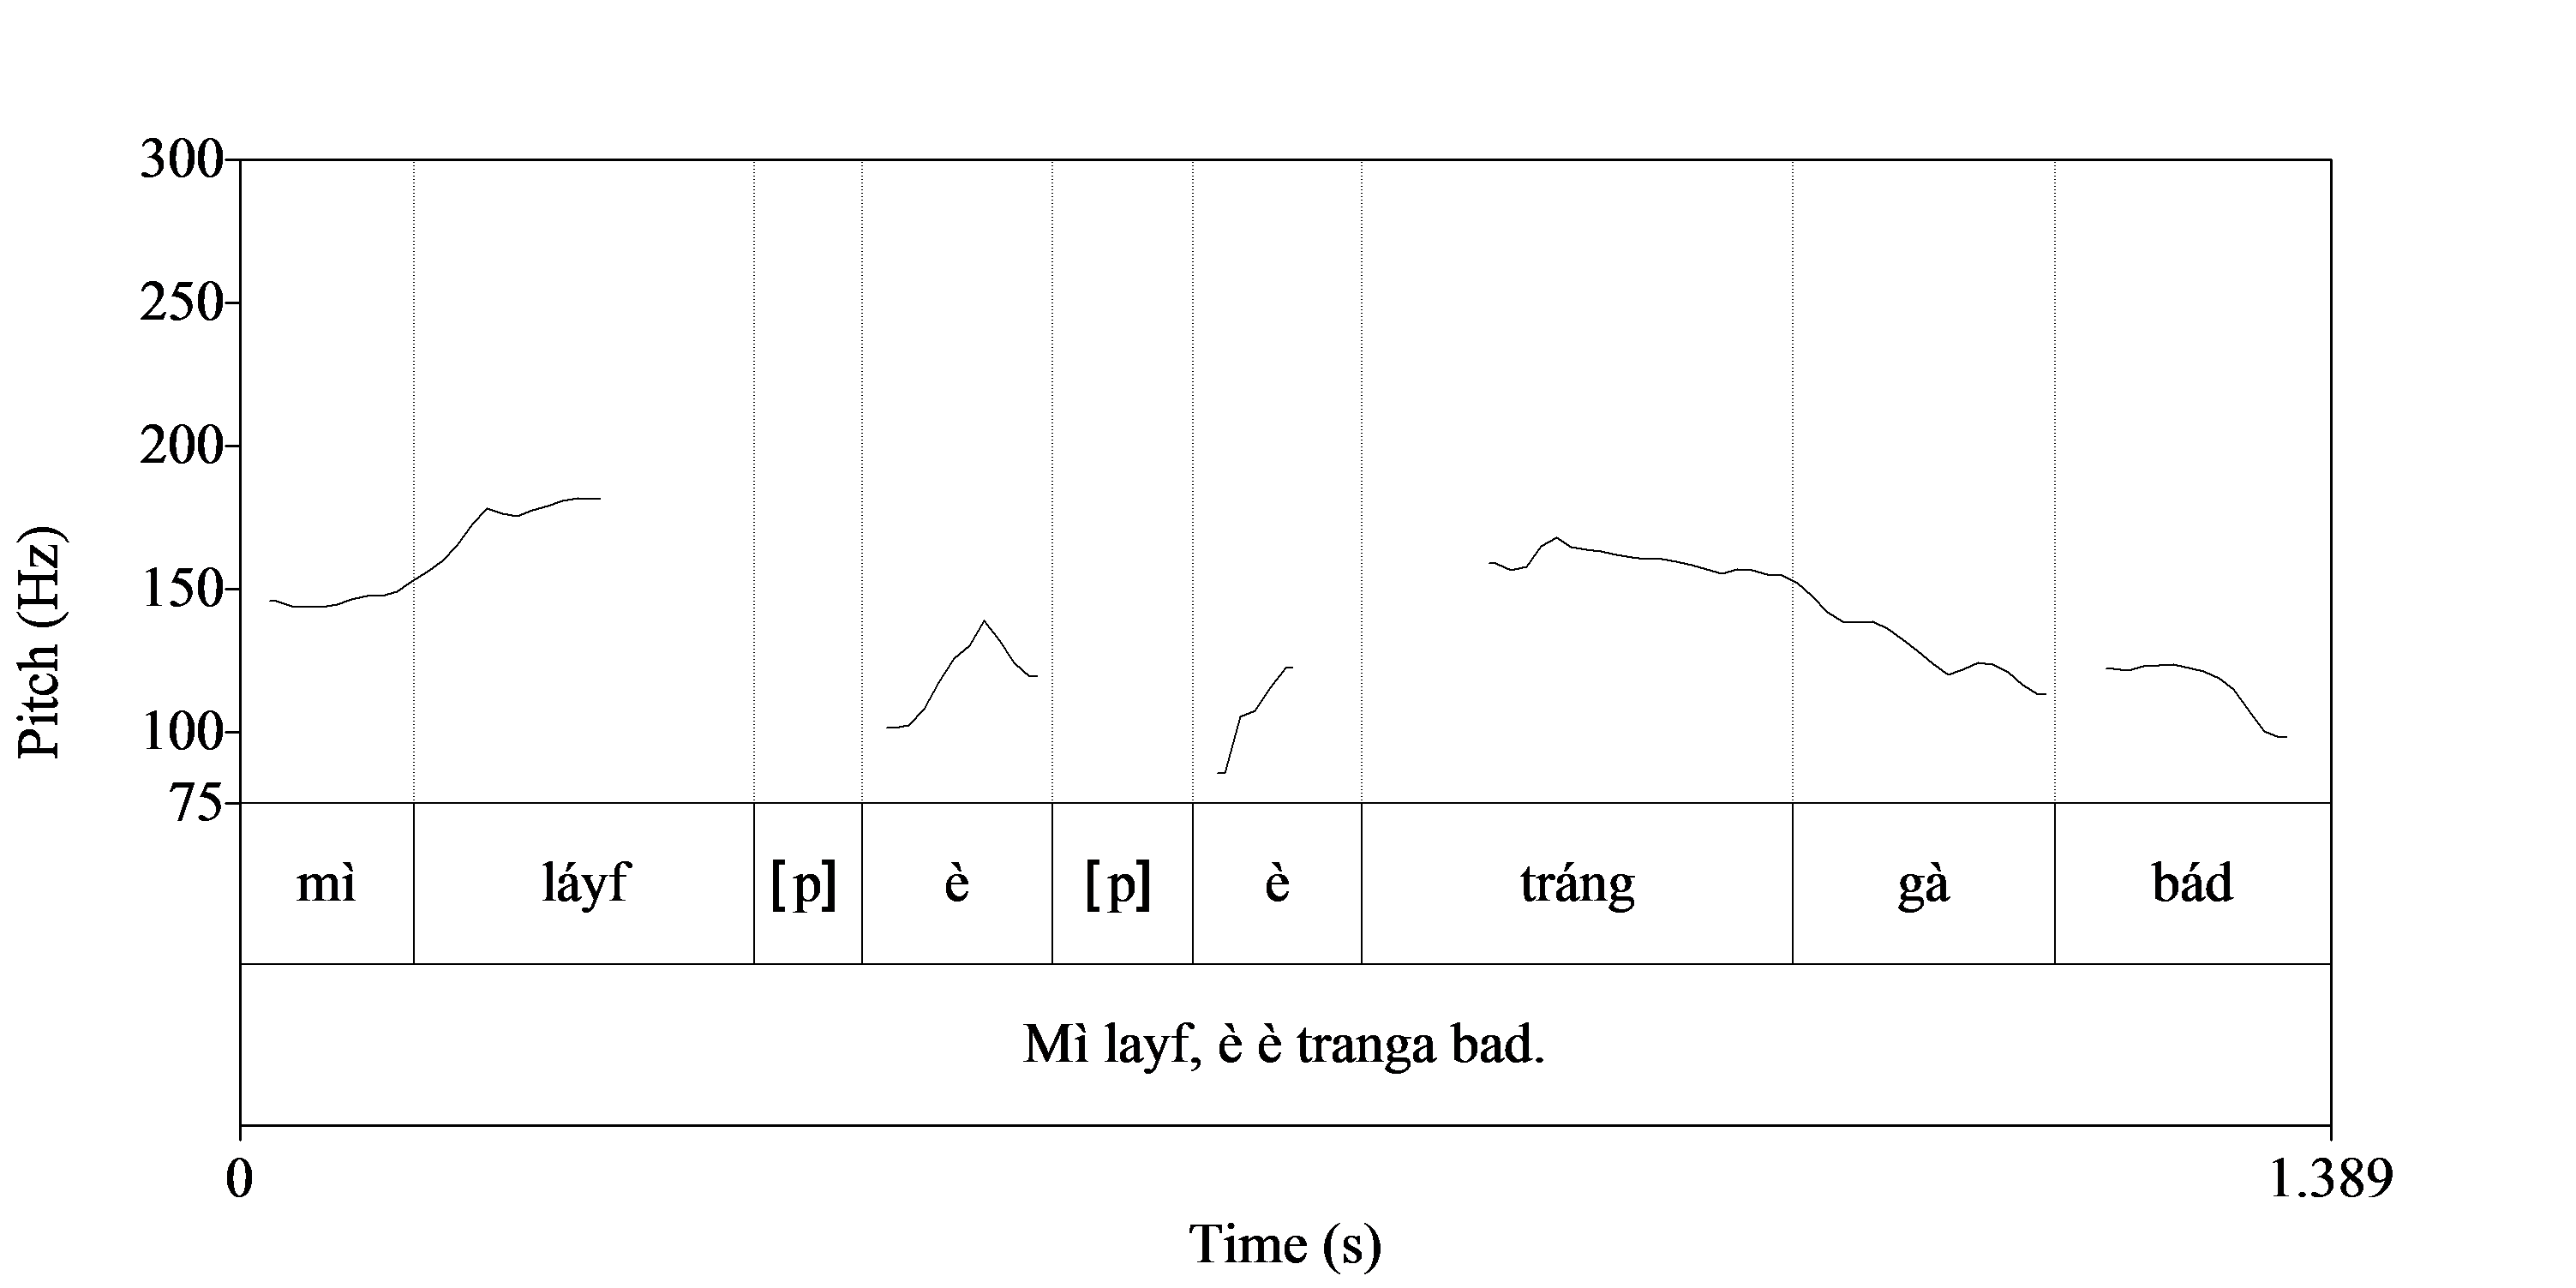
\includegraphics[height=.3\textheight]{figures/yakpomod-img41.png}
\end{figure}

  
 
\ea\label{ex:key:92}
\glll Mi \textstylePichiexamplebold{láyf},  e,    e    tránga \textbf{bád}.\\
\textsc{l}    \textsc{h}\textbf{\textsc{${\emptyset}$}}\textbf{\textsc{\%}  }  \textsc{l}    \textsc{l}    \textsc{h.l}      \textsc{h}\textbf{\textsc{l\%}}\\
\textsc{1sg.poss}  life    \textsc{3sg.sbj}  \textsc{3sg.sbj}  be.strong  extremely\\
\glt ‘My life, it, it was really tough.’    
\z

Continuative intonation is also employed as a juncture marker between linked clauses. Here, it may occur alone as a prosodic clause linker between juxtaposed clauses, or in conjunction with an overt clause linker. \figref{fig:key:3.40} and \figref{fig:key:3.41} are two clauses linked in a sequential, temporal relation. The adverbial time clause is introduced by \textit{di} \textit{dé} \textit{wé} ‘(the day) when’ in \figref{fig:key:3.40}. In the example, continuative intonation is found over the rightmost L-toned monosyllable \textit{=an} ‘\textsc{3sg.obj}’. The absence of the utterance-final L\% of declarative intonation halts the fall of the lexical L tone to the bottom of the pitch register:

\begin{figure}
\caption{Continuative intonation with clause linkage} 
\label{fig:key:3.40}
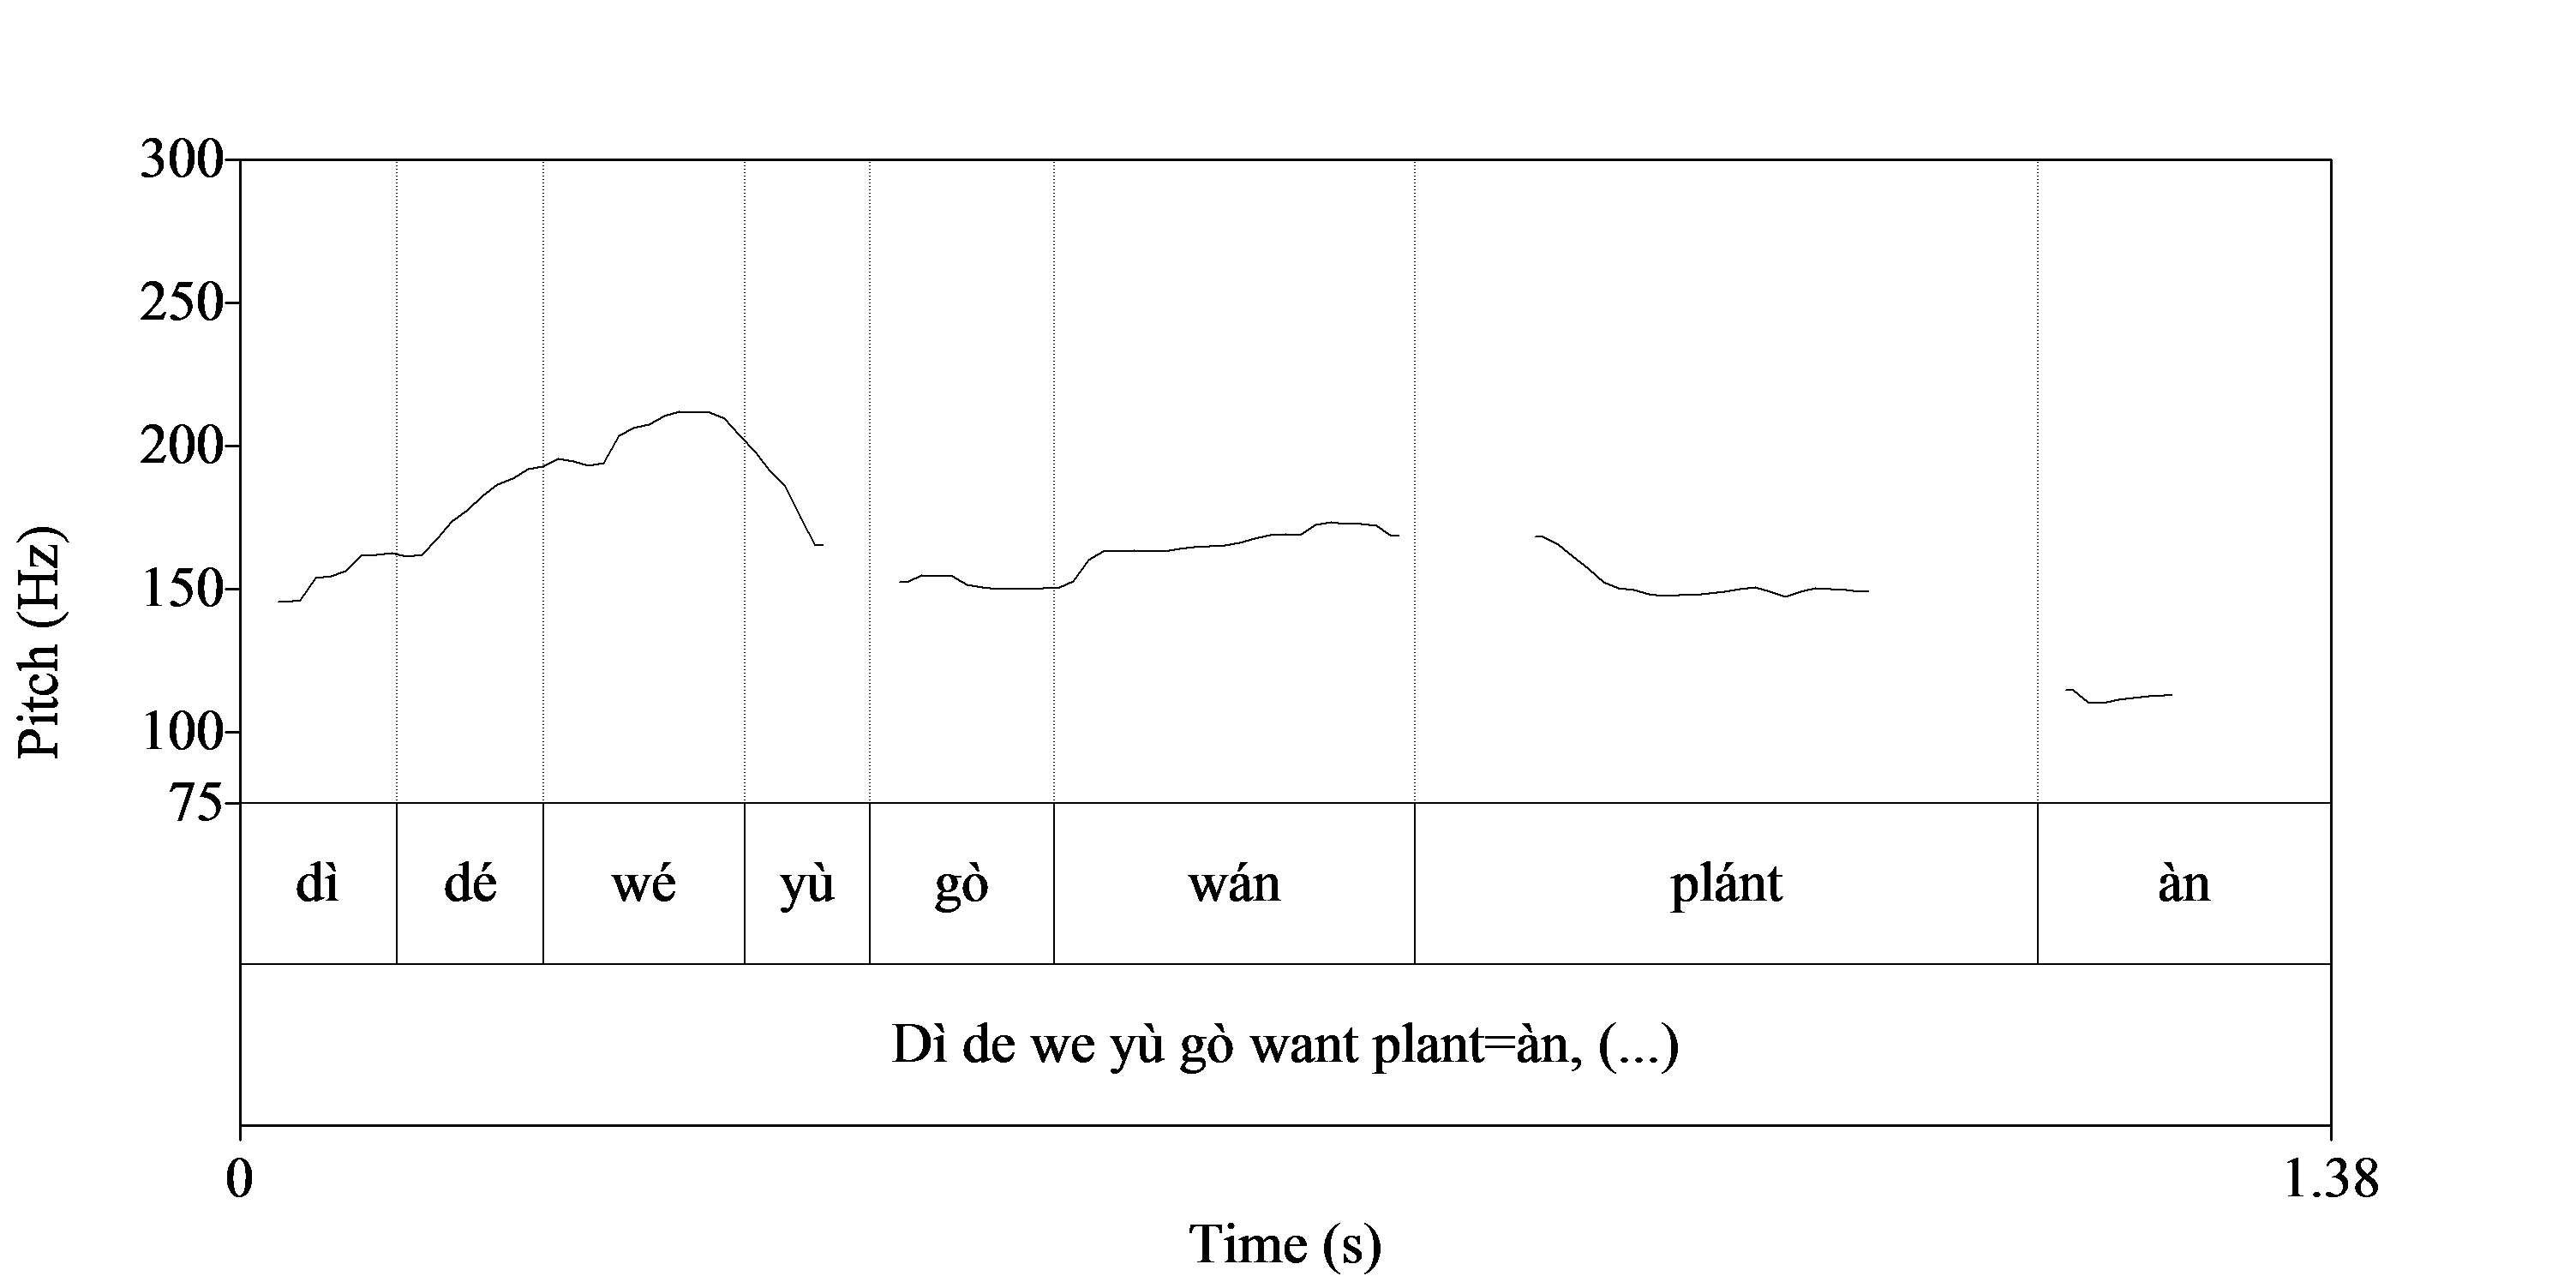
\includegraphics[height=.3\textheight]{figures/yakpomod-img42.png}
\end{figure}

\ea%93
    \label{ex:key:93}
    \glll   Di  dé  wé  yu  go  wánt  plánt=an,  (...)\\
\textsc{l}  \textsc{h}  \textsc{h}  \textsc{l}  \textsc{l}  \textsc{h}    \textsc{h=l}\textbf{\textsc{${\emptyset}$}}\textbf{\textsc{\%}}\\
\textsc{def}  day  \textsc{sub}  \textsc{2sg}  \textsc{pot}  want  plant=\textsc{3sg.obj}\\
\glt ‘The day you would want to go plant it (...)’      
\z

The second clause in sequence features a lexical H over the utterance-final syllable. Here, continuative intonation produces no effect other than the maintenance of the lexical H tone. Compare \textit{dɔtalɔ́} ‘daughter-in-law’ and \textit{sɔnilɔ́} ‘son-in-law’ in \figref{fig:key:3.41}: 

\begin{figure}
\caption{Continuative intonation over non-final clause}
\label{fig:key:3.41}
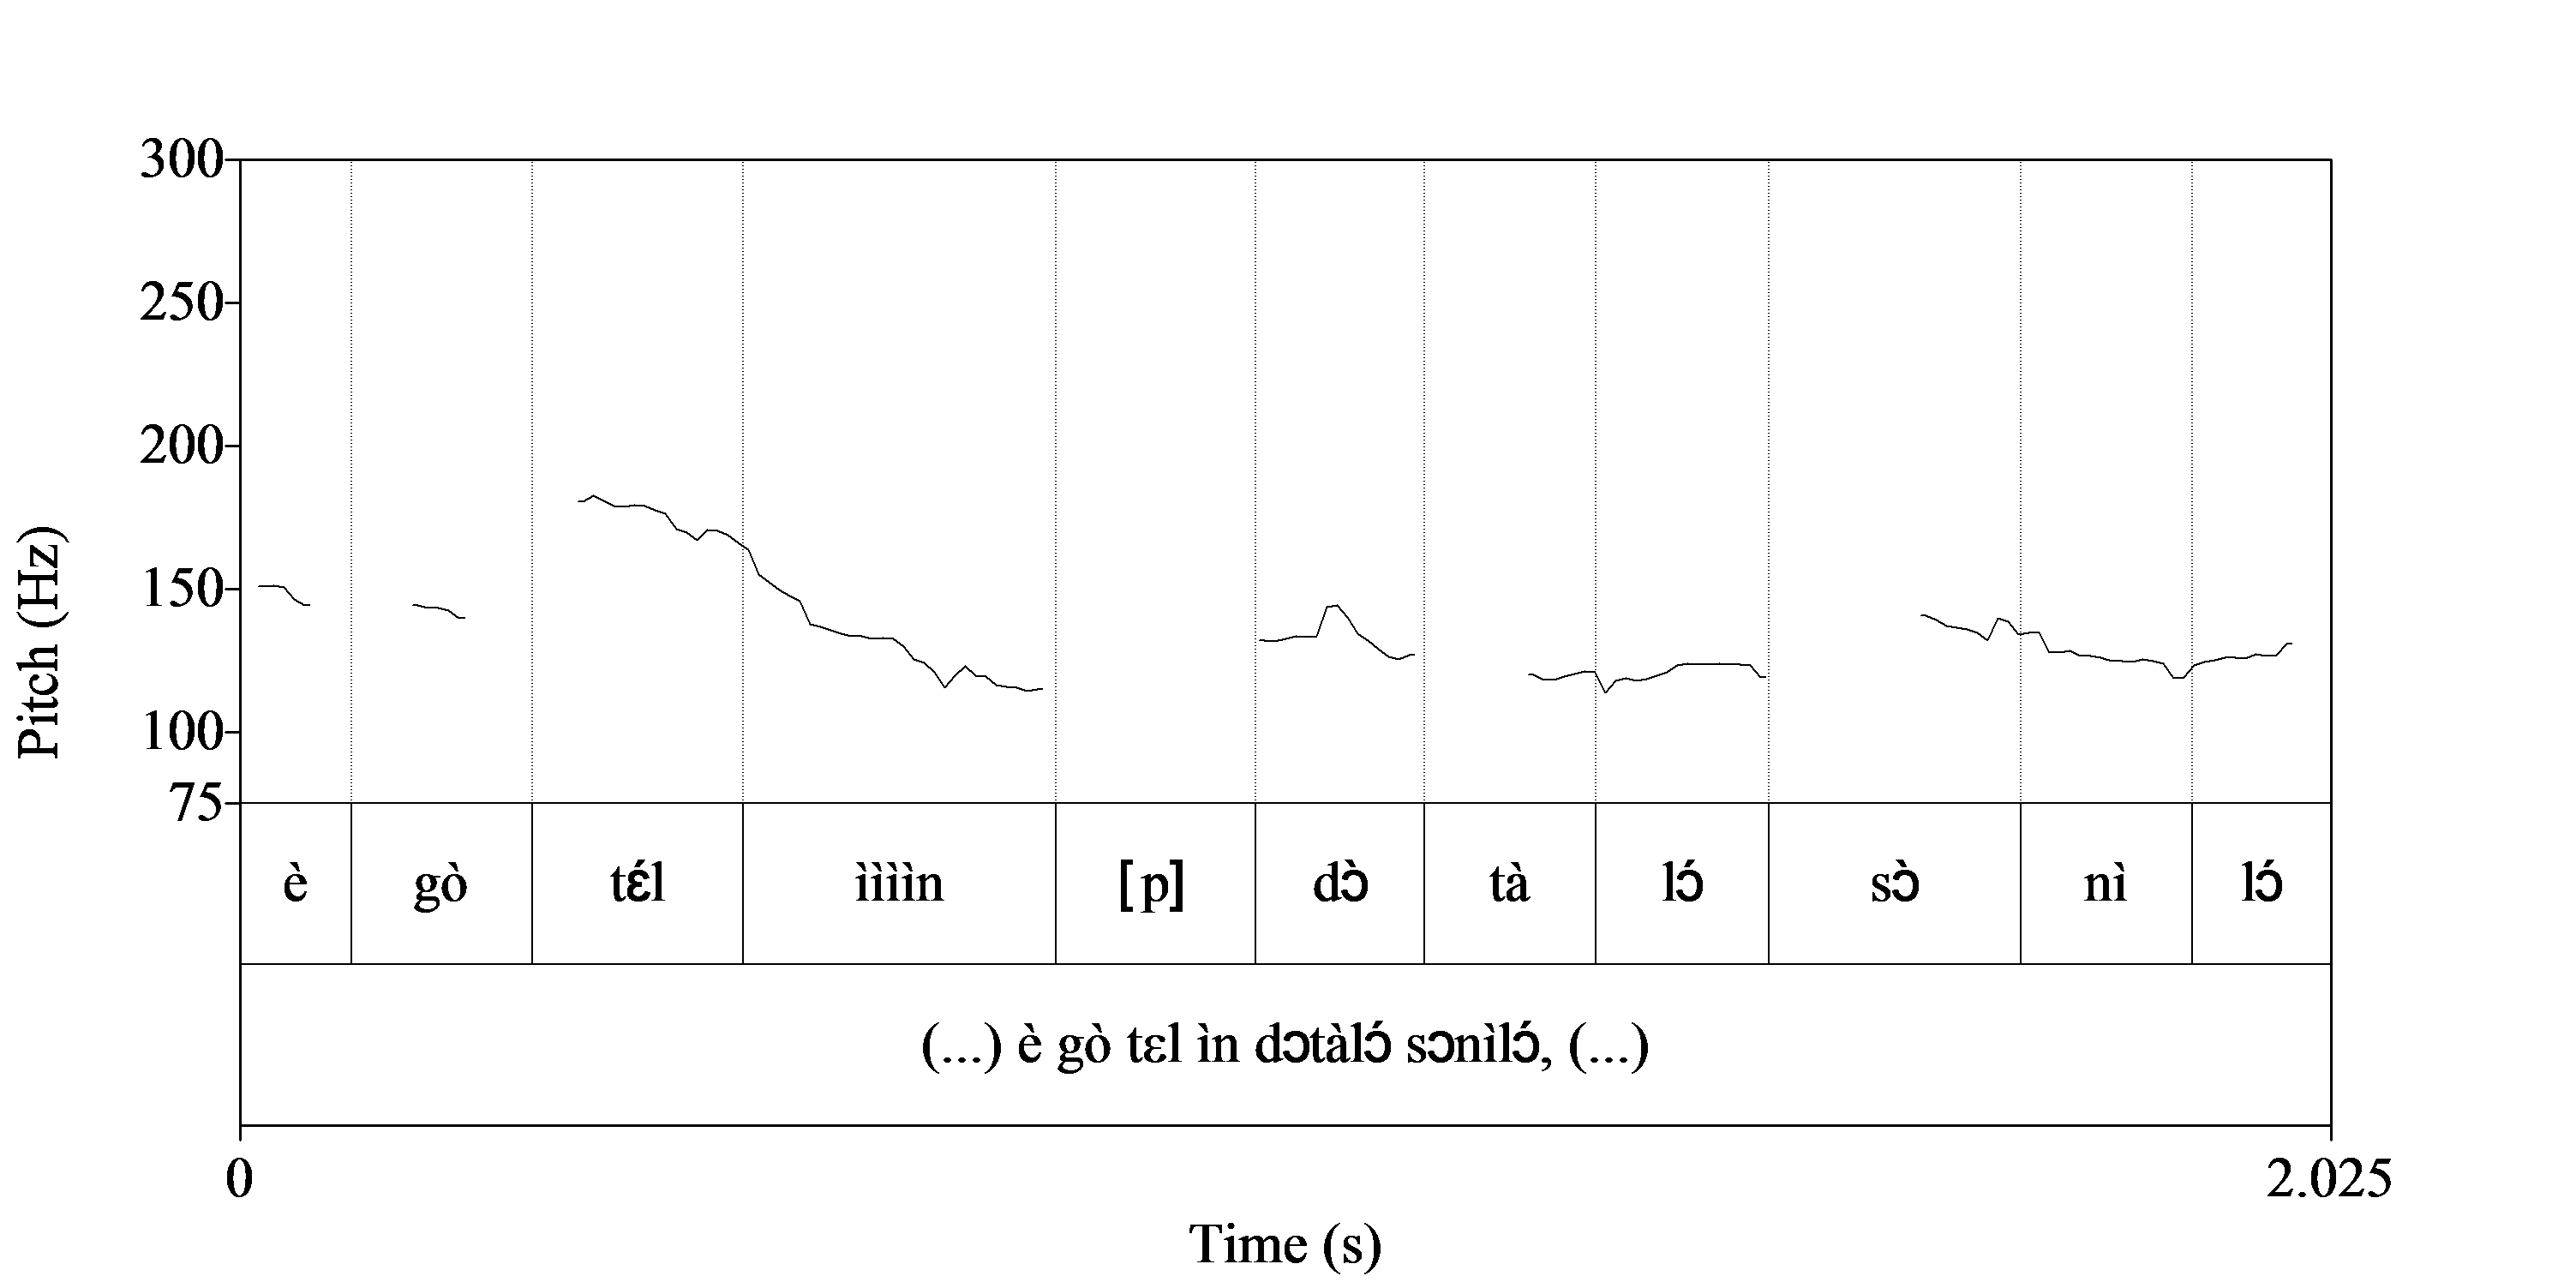
\includegraphics[height=.3\textheight]{figures/yakpomod-img43.png}
\end{figure}

\ea%94
    \label{ex:key:94}
    \glll   E    go  tɛ́l  in    dɔtalɔ́,      sɔnilɔ́,  (...)\\
\textsc{l}    \textsc{l}  \textsc{h}  \textsc{l}    \textsc{l.l.h}\textbf{\textsc{${\emptyset}$}}\textbf{\textsc{\%}}      \textsc{l.l.h}\textbf{\textsc{${\emptyset}$}}\textbf{\textsc{\%}}\\
\textsc{3sg.sbj}  \textsc{pot}  tell  \textsc{3sg.poss}  daughter-in-law  son-in-law\\
\glt ‘She would tell her daughter-in-law, son-in-law, (...)’  
\z


Continuative intonation is also used as a stylistic device in ‘unfinished’\textstyleannotationreference{} utterances, such as the one in \figref{fig:key:3.42}. The final syllable retains its H tone or may even rise slightly towards the end. This emphatic variant of declarative\is{declarative intonation:emphatic} intonation is employed for dramatic effect. Compare the utterance-final, H-toned monosyllable \textit{dé} ‘there’: 

\begin{figure}
\caption{Continuative intonation for stylistic effect}
\label{fig:key:3.42}
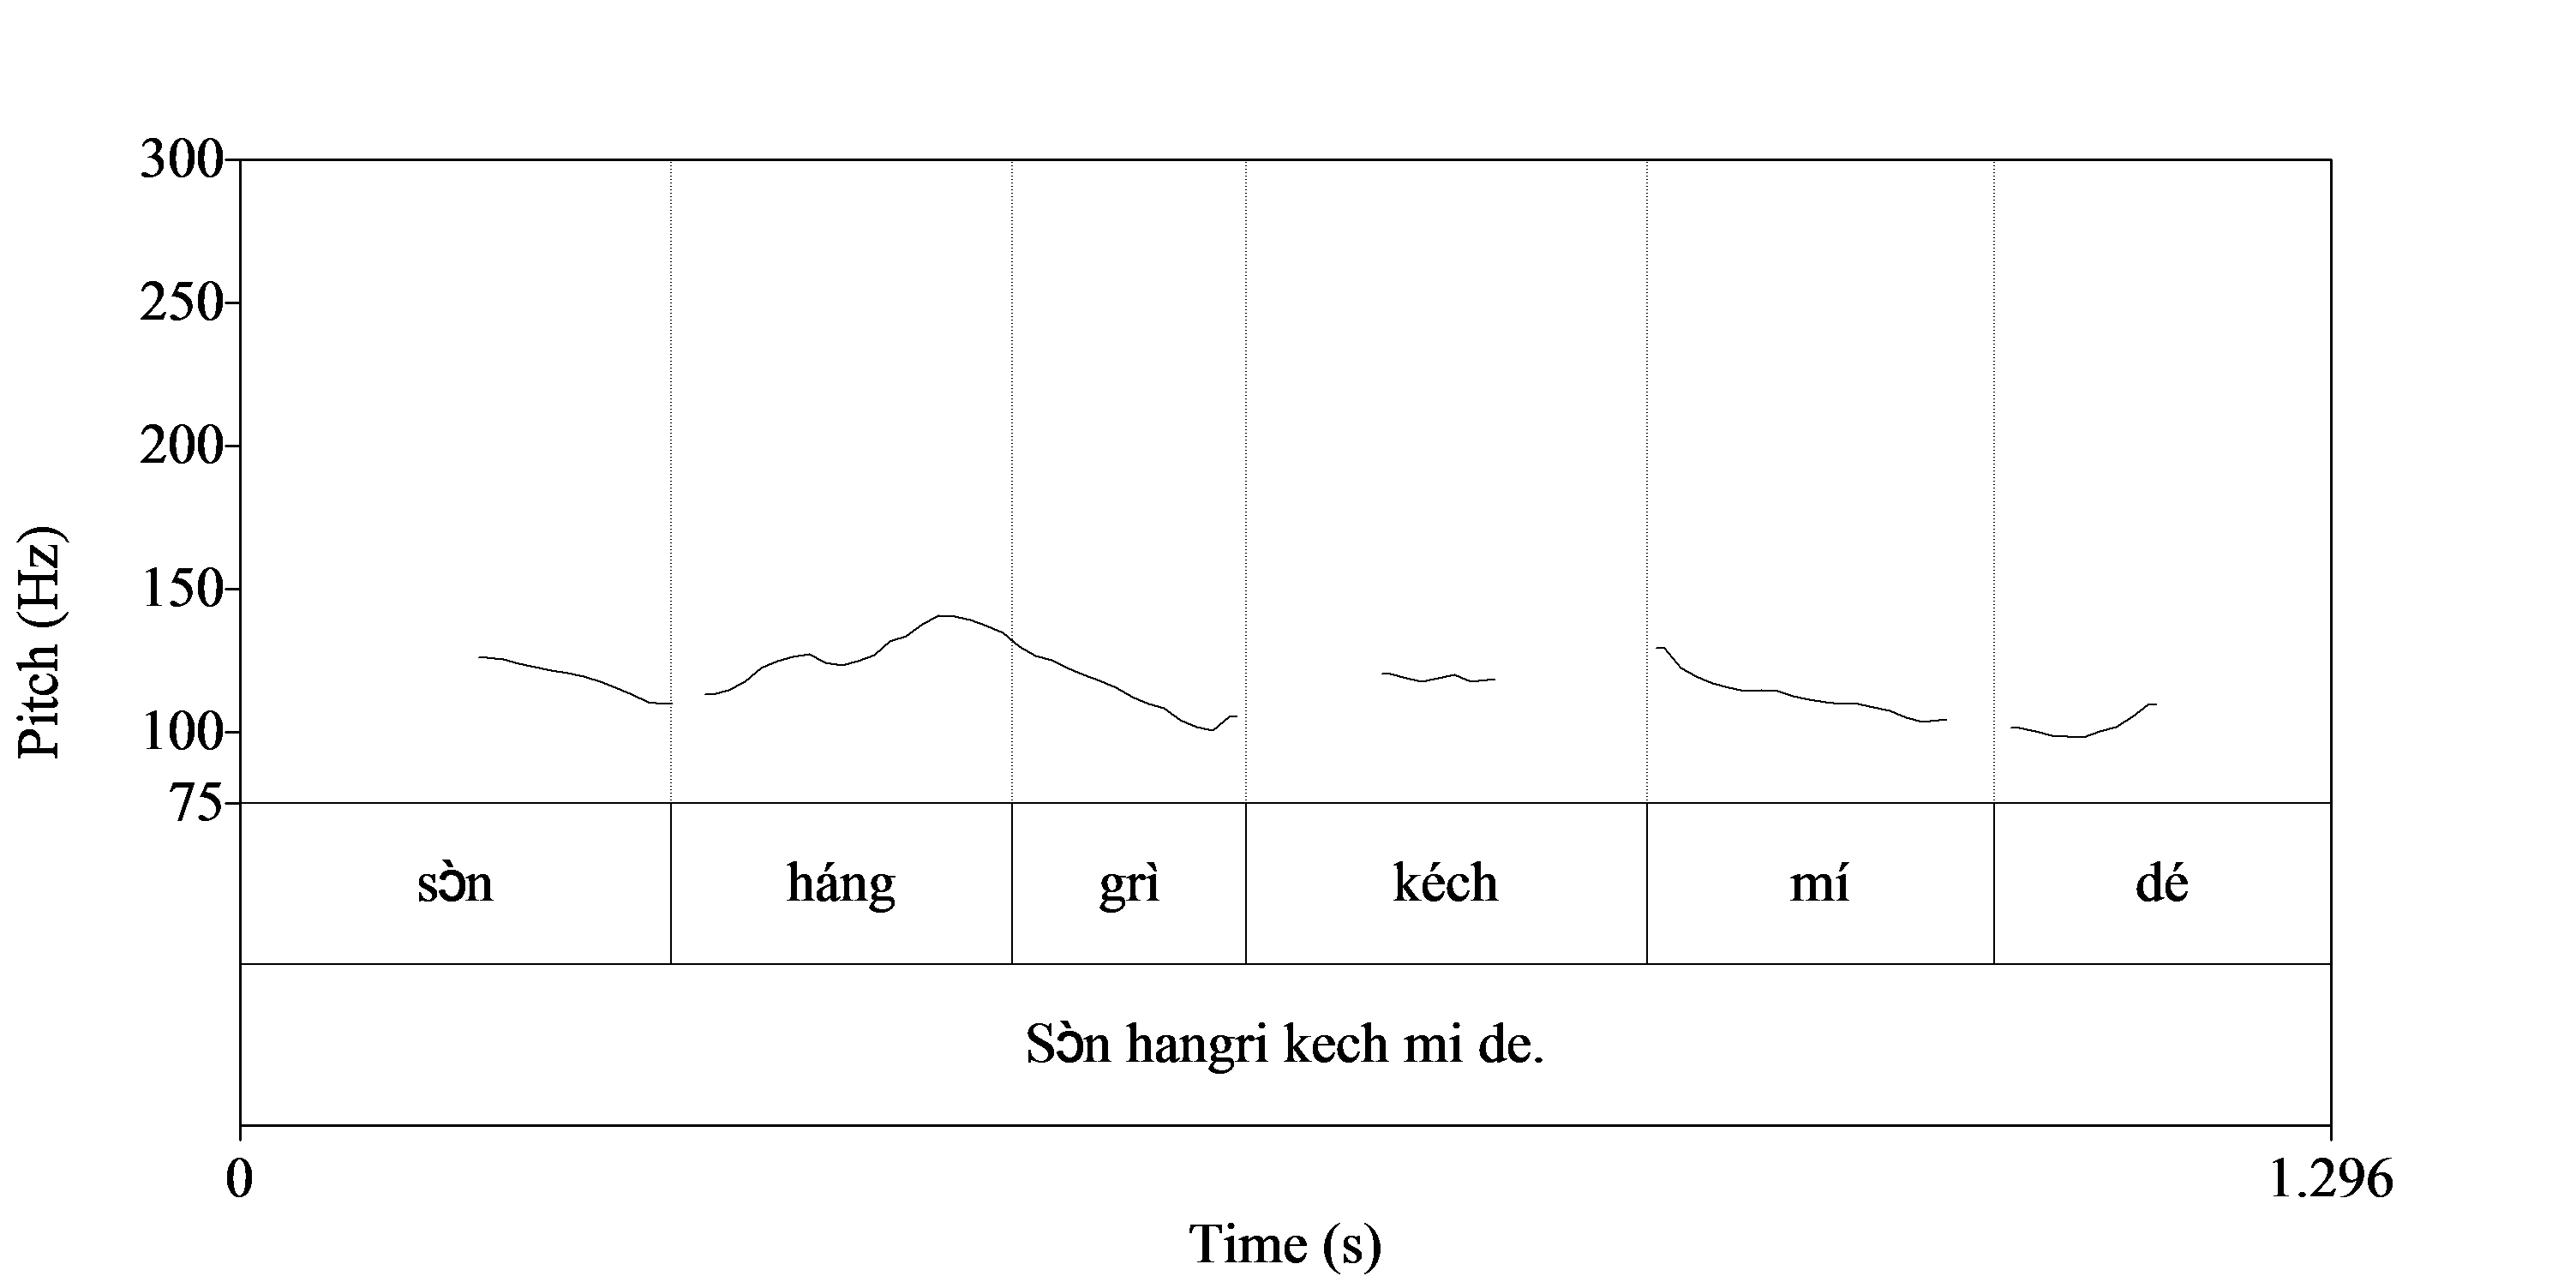
\includegraphics[height=.3\textheight]{figures/yakpomod-img44.png}
\end{figure}

  
 


\ea%95
    \label{ex:key:95}
    \glll   Sɔn    hángri    kéch  mí    \textbf{dé}.\\
L    \textsc{h.l}      \textsc{h}    \textsc{h}    \textsc{h}\textbf{\textsc{${\emptyset}$}}\textbf{\textsc{\%}}\\
some  be.hungry  catch  \textsc{1sg.indp}  there\\
\glt ‘I became really hungry there [you wouldn’t believe how much].’\is{continuative intonation}
\z

\subsection{Question intonation}\label{sec:3.4.5}

Yes–no questions are formed with an LH\% contour boundary tone. Contrary to emphatic intonation, question intonation is substitutive: The lexical tone over the utterance-final syllable is replaced by the question LH\%. In this way, the utterance-final syllable of a yes–no question invariably bears an LH contour, irrespective of its original tone. Compare the pitch contour over the L-toned second syllable of \textit{Píchi} ‘Pichi’ in \figref{fig:key:3.43}: 

\begin{figure}
\caption{Non-emphatic yes–no question}
\label{fig:key:3.43}
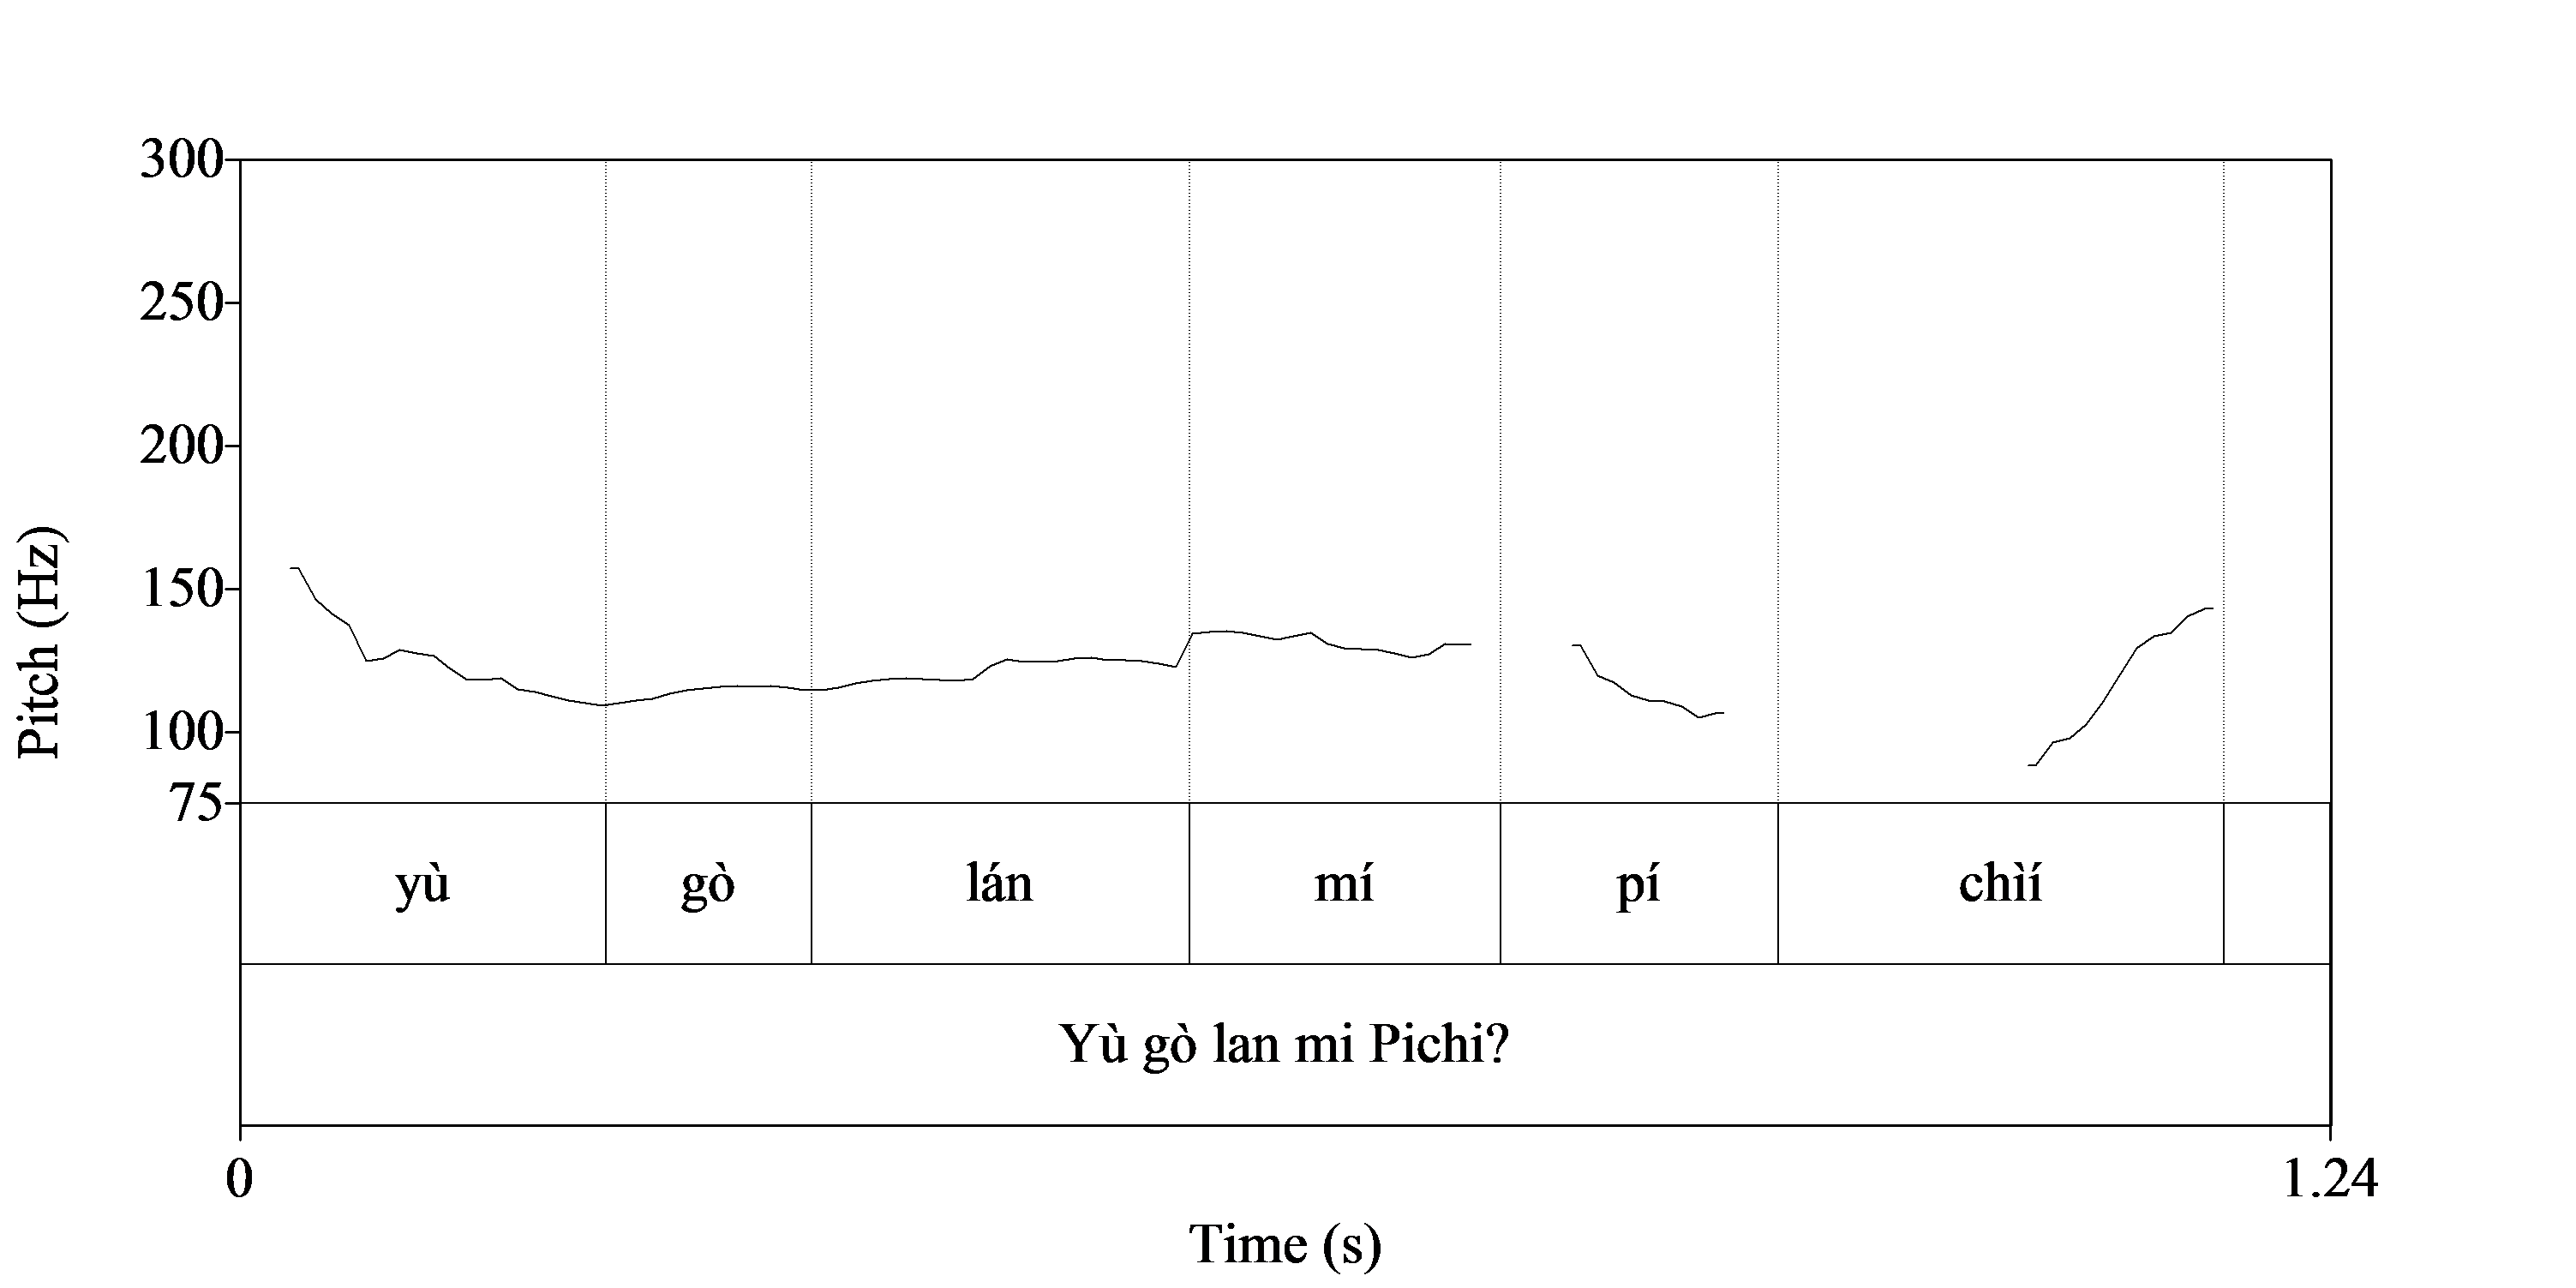
\includegraphics[height=.3\textheight]{figures/yakpomod-img45.png}
\end{figure}

  
 


\ea%96
    \label{ex:key:96}
    \glll   Yu    go    lán    mí    Píchi?\\
\textsc{l}    \textsc{l}    \textsc{h}    \textsc{h}    \textsc{h.}\textbf{\textsc{lh\%}}\\
\textsc{2sg}    \textsc{pot}    teach  \textsc{1sg.indp}  Pichi\\
\glt ‘Will you teach me Pichi?’  
\z

The H tone of the LH\% contour may vary in pitch. While non-emphatic questions exhibit a gentle final rise and may therefore be similar in pitch to continuative intonation\is{continuative intonation}, more emphatic questions yield steeper rises. The more dramatic the rise, the more the question may additionally convey emphatic nuances like counter-expectation or insistence. I assume that in instances where the rise is particularly steep, the H tone component of the LH\% boundary contour tone is raised to extra-high, thus rendering L+H\%. Such an extra-steep rise is particularly common in rhetorical questions, optionally over the L-toned utterance-final question tag \textit{nɔ́} as in the following example:\is{alternative questions} 

\begin{figure}
\caption{Emphatic yes–no question}
\label{fig:key:3.44}
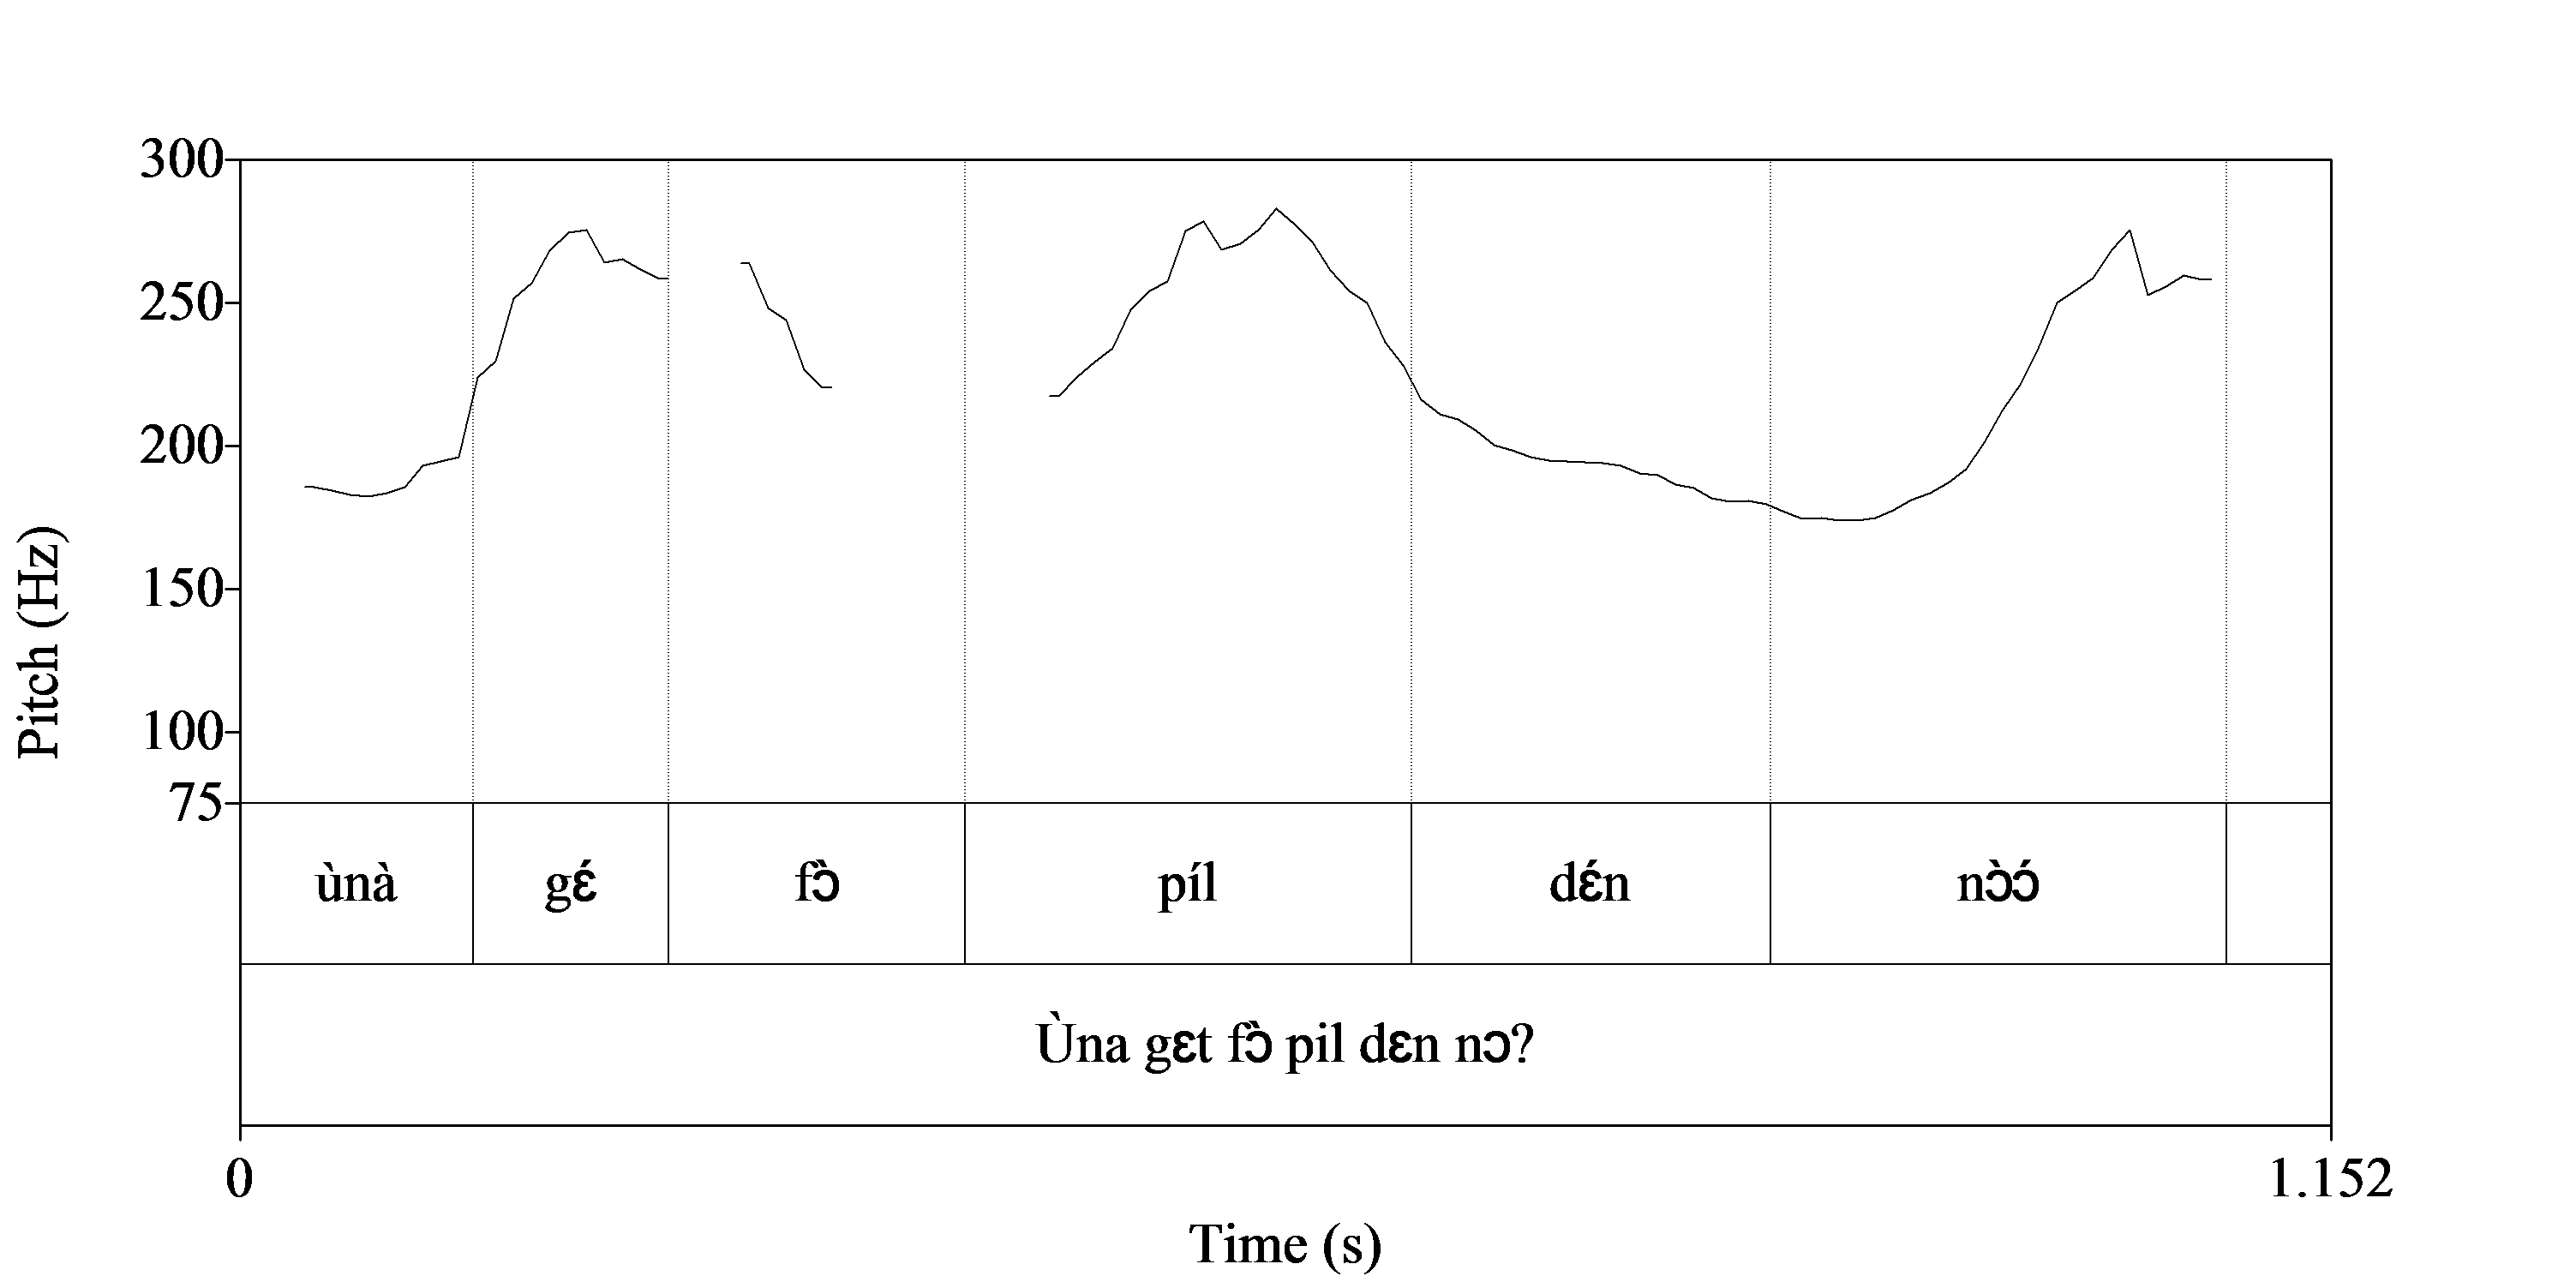
\includegraphics[height=.3\textheight]{figures/yakpomod-img46.png}
\end{figure}

  
 


\ea%97
    \label{ex:key:97}
    \glll   Una    gɛ́fɔ    píl    dɛ́n    nɔ́?\\
\textsc{l.l}    \textsc{h.l}    \textsc{h}    \textsc{l}    \textbf{\textsc{l+h\%}}\\
\textsc{2pl}    have.to  peel    \textsc{3pl.indp}  right\\
\glt ‘You [\textsc{pl}] have to peel them, right [you should know that]?’
\z



The utterance-final syllable in the question above exhibits a particularly steep rise. At the same time, emphasis\is{emphasis} is additionally expressed through pitch range expansion. The contrast between H and L tones is widened across the entire utterance as can be seen by the deep troughs in the pitch trace.\is{question intonation}


\chapter{Morphology}

Pichi nouns and verbs constitute two major word classes. Adjectives, prepositions, and adverbs constitute minor word classes with a few members each. Pichi word formation strategies are predominantly analytic. Besides that, the use of one (adverb-deriving) affix and morphological tone play a role in Pichi derivation and inflection.

\section{Word classes}\label{sec:4.1}

Pichi word classes are differentiated by their syntactic functions (e.g. a noun may head an \textsc{NP}), distribution within the sentence (e.g. a preposition may not be preceded by an article), the morphosyntactic categories that may be specified for them (e.g. verbs may be specified for tense\is{tense}, \isi{aspect}, and \isi{modality}), their derivational potential (e.g. personal pronouns and prepositions are not normally reduplicated, and adverbs do not function as nouns), as well as semantic criteria (dynamic states-of-affairs and property concepts are generally expressed as verbs). 


The major underived word classes, with the most members and the potential to occur in the largest range of environments, are nouns and verbs. The noun-verb distinction in Pichi is quite strong: although verbs may function as nouns in specific (e.g. in emphatic) contexts, the reverse is not usually the case. The verb-adjective distinction is weak. There are only a handful of adjectives, which are indistinguishable from verbs in most environments. The minor word classes consist of adjectives, prepositions, adverbs, as well as various sentence elements that contribute to the meaning of the sentence. 


\subsection{Nominals}

Nouns appear as one of up to three core participant\is{core participants}s of a verb, i.e. as subjects or up to two objects\is{objects}. Nouns also occur as objects of prepositions, and they may function as adverbials. They may be modified by other elements of the noun phrase (e.g. \textit{di} ‘\textsc{def}’, \textit{dá(n)} ‘that’, \textit{sɔn} ‘some, a’ or \textit{dɛn} ‘\textsc{pl’)}, including other nouns in associative constructions and compounds. \is{associative constructions}The vast majority of nouns bears a single H tone and belongs to one of the major tone classes (cf. \tabref{tab:key:3.2}). Underived nouns typically denote time-stable object concepts. Nouns also belong to an open class which may be extended by compounding, conversion, and borrowing\is{borrowing} from \ili{Spanish}.


Personal pronouns, pronominals, and compound question word{\fff}s are subsets of nominals that exhibit a more restricted distribution. Personal pronouns are found in the same syntactic positions as noun phrases but do not cooccur with preposed modifiers. The latter usually also holds true for the pronominals \textit{nátin} ‘nothing’, \textit{sɛ́f} ‘self’, and \textit{yón} ‘own’. The pronominals \textit{káyn} ‘kind’ and \textit{wán} ‘one’ have a wider distribution but are also characterised by specific syntactic preferences. Locative nouns{\fff} form a further subclass of nominals characterised by distributional specificities. Locative nouns are not often preceded by modifiers or determiners, and their distribution overlaps with that of prepositions. 


\subsection{Verbs and adjectives}\label{sec:4.1.2}

Verbs occupy the centre of the predicate. The predicate is best seen to include a number of functional elements that form a tightly-knit unit with the verb in order to constitute clauses: TMA markers, preverbal adverbs\is{preverbal adverbs}, the negator, dependent personal pronouns, as well as the clitic \textsc{3sg} object pronoun. Verbs are usually preceded by a subject noun, pronoun, or both. Verbs may optionally be followed by objects\is{objects}. They are typically mono- or bisyllabic and usually belong to one of the three major tone classes. 


There are numerous subclasses of verbs which can be defined along formal and semantic lines: Aspectual and modal verbs, transfer and communication verbs, stative, inchoative-stative, and dynamic verbs, labile verbs{\fff}, and copula verbs. Other than reduplication, Pichi only has marginally productive means of verb derivation through compounding{\fff}. There are numerous other strategies for the creation of new verbal meanings, e.g. light verb constructions, involving \textit{gɛ́t} ‘get, have’, \textit{mék} ‘make’, or \textit{gí} ‘give’, as well as systematic borrowing{\fff} from Spanish.



There is just a handful of adjectives in Pichi. A small set of property items alternates between uses as inchoative-stative verbs and as adjectives (cf. \tabref{tab:key:7.11} in \sectref{sec:7.6.5}). {\fff}The overwhelming majority of property concepts are lexicalised as inchoative-stative verbs in Pichi. The following “semantic types” \citep[3]{dixon_adjective_2004} are expressed through inchoative-stative verbs: Dimension (e.g. \textit{bíg} ‘be big’, \textit{smɔ́l} ‘be small’, and \textit{lɔ́n} ‘be long’), age (e.g. \textit{ól} ‘be old’ and \textit{yún} ‘be young’), value (e.g. \textit{bád} ‘be bad’, \textit{fáyn} ‘be good’, and \textit{trú} ‘be true’), and colour (e.g. \textit{blák} ‘be black’, \textit{wáyt} ‘be white’, \textit{rɛ́d} ‘be red’, and \textit{yɛ́lo} ‘be yellow’). Most physical properties are also lexicalised as inchoative-stative verbs (e.g. \textit{hád} ‘be hard’, \textit{sáf} ‘be soft’, \textit{sók} ‘be wet’, \textit{évi} ‘be heavy’, \textit{hɔ́t} ‘be hot’, \textit{swít} ‘be tasty’). 



Human propensities are divided between inchoative-stative (e.g. \textit{gudhát} ‘be good-hearted’, \textit{wíkɛd} ‘be wicked’, \textit{badhát} ‘be mean’, \textit{klɛ́va} ‘be clever’) and dynamic verbs (e.g. \textit{gládin} ‘be glad’, \textit{jɛ́lɔs} ‘be envious’) according to whether they denote intrinsic or transient properties. Resultatives{\fff} are exclusively expressed through the stative readings of labile change-of-state verbs (e.g. \textit{brók} ‘break, be broken’, \textit{chɛ́r} ‘tear, be torn’, \textit{lɔ́s} ‘lose, be lost’ and \textit{wɛ́r} ‘be dressed’). Semantic types like position or location are expressed through other means, such as copula clauses featuring the locative-existential copula \textit{dé} (cf. e.g. \ref{ex:key:793}–\ref{ex:key:794}) in combination with adverbials, or through locative verbs like {\fff}\textit{lé} ‘lie’ and \textit{tínap} ‘stand (up)’ (cf. \sectref{sec:8.1.3}).


\subsection{Other word classes}\label{sec:4.1.3}

Most prepositions must be followed by an object, although some may be stranded\is{stranding}, that is, they may occur in the clause-final position. Prepositional phrases are found in the clause-initial or -final position. A majority of prepositions is monosyllabic, a few are bisyllabic. Pichi exhibits a division of labour between prepositions, locative nouns, locative adverbs, and locative verbs in order to express spatial relations. The language has a small number of underived adverbs, amongst them a group of four preverbal adverbs\is{preverbal adverbs}.


Each of the following groups of modifiers may also be said to constitute minor word classes unto themselves, because they occupy distinct syntactic positions in the noun phrase or predicate: the article, demonstratives, quantifiers, prenominal attributive modifiers, numerals, the pluraliser\is{pluraliser}, emphasis markers, topicalisers, TMA markers, aspectual and modal verbs, the general negator, interjections, and ideophones\is{ideophones}. Certain elements modify sentences in their entirety with respect to pragmatic status (e.g. question words, tags, focus particles, interjections) or link sentences with each other (e.g. clause linkers and conjunctions). These sentential elements may also each be considered a separate word class due to their functions and syntactic behaviour.\is{word classes} 


\section{Inflection}\label{sec:4.2}

Most grammatical functions are realised analytically by independent words without the morphological modification of heads or dependents. Participant-marking is taken care of by prepositions and locative nouns, serial verb constructions, and word order, and nominal modification by juxtaposition of adjectives and other modifiers\is{word orderes}. Number-marking is achieved by post-nominal modification. 

The verbal category of number is signalled by personal pronouns and reduplication. Complementisers, preverbal TMA markers, serial verb constructions, and adverbs participate in expressing the grammatical categories of tense{\fff}, modality, and aspect. Comparison is expressed by adverbs of degree, ideophones, verbs, phrasal expressions, suprasegmental modification, serial verb constructions, and prepositions. There are, however, exceedingly rare cases of number marking on \textit{gɛ́l/gál} ‘girl’ and \textit{bɔ́y} ‘boy’ by an apparently marginal plural affix \{-s\}, hence \textit{gɛ́l-s}, \textit{bɔ́y-s}. 


A description of the only inflectional morphological processes follows. The expression of the grammatical relations of subject, object, and possessive case may be seen to involve the use of (tonal) suprafixation, summed up in \tabref{tab:key:4.1} (cf. \sectref{sec:5.4.1} for the full pronominal paradigm and examples).


%%please move \begin{table} just above \begin{tabular
\begin{table}
\caption{Suprafixation with personal pronouns}
\label{tab:key:4.1}

\begin{tabularx}{.75\textwidth}{Xl}
\lsptoprule

Category expressed & Suprafix\\
\midrule
Object case \& independent pronouns & H tone\\
Subject \& possessive case & L tone\\
\lspbottomrule
\end{tabularx}
\end{table}

Tone-conditioned suppletive allomorphy also fulfils inflectional functions in Pichi, even if it involves outright substitution rather than morphological modification (cf. \sectref{sec:3.3}). It has been suggested that the cognate form of the Pichi imperfective marker \textit{de} ‘\textsc{ipfv}’ be analysed as an inflectional verbal prefix in Jamaican Creole \citep[30]{Farquharson2007}. In Pichi too, the use of resumptive imperfective marking with the preverbal aspectual adverbs \textit{jís/jɔ́s} ‘just’ and \textit{stíl} ‘still’ suggests a tighter-than-usual syntagmatic relation between the imperfective aspect marker and the verb it modifies:


\ea%98
    \label{ex:key:98}
    \gll   Náw    dɛn  \textbf{de}  \textbf{jís}  \textbf{de}  kán.\\
now    \textsc{3pl}  \textsc{ipfv}  just  \textsc{ipfv}  come\\

\glt ‘Now, they’re just coming.’ [ye07je 179] \is{preverbal adverbs}
\z

\section{Derivation}\label{sec:4.3}

Pichi makes use of morphological processes for the purpose of derivation. One is a tonal process which derives compounds, including reduplications. The other is adverb-deriving suffixation. Compounding and reduplication are two highly productive derivational processes in Pichi. 

\subsection{Affixation}
\tabref{tab:key:4.2} summarises the derivational processes found in Pichi. This section covers formal aspects of compounding and reduplication, which both receive a more detailed functional treatment in \sectref{sec:4.4} and \sectref{sec:4.5.1}, respectively. Adverb-deriving suffixation is covered in this section in both its formal and functional aspects.

%%please move \begin{table} just above \begin{tabular
\begin{table}
\caption	{Derivational processes}
\label{tab:key:4.2}
{\small\begin{tabularx}{\textwidth}{QQ lQ l}
\lsptoprule
Category expressed & Word class applied to & (Supr-)affix & Process & Productivity\\
\midrule
Verbal plurality & Dynamic verbs & L tone + \textsc{red} & Tone deletion + iteration & High\\

\tablevspace
Nominal and verbal compound & Nouns, pronouns verbs, adverbs, phrases & L tone & Tone deletion & Fair\\

\tablevspace
Manner adverb & Verbs, adjectives & {}-\textstyleTablePichiZchn{wán} \textsc{‘adv’} & Suffixation & Low\\
\lspbottomrule
\end{tabularx}}
\end{table}

Compounding and reduplication both make use of the same tonal derivation. Reduplication is therefore best seen as a form of (self-)compounding in Pichi. In the process, the H tone over the initial component(s) is deleted and replaced by an L tone. The final component retains its original tone configuration. The resulting compound word then features a single H tone like most Pichi words. Pichi compounds are therefore right-headed; the L-toned initial component(s) function as modifier(s) to the final component, which is the head. 


Nouns, verbs, adjectives, and adverbs participate in compounds. The resulting structures may function as nouns or verbs. Personal pronouns may also participate as modifiers in compound personal pronouns (cf. \sectref{sec:5.4.2}). Compounding is fairly productive (cf. \sectref{sec:4.4} for details). Compare the compound in \REF{ex:key:99} featuring the modifier noun \textit{kɔ́ntri} ‘country, home town’ and the modified noun \textit{chɔ́p} ‘food’. While \textit{kɔ́ntri} loses the H tone over its first syllable, the head noun \textit{chɔ́p} retains its original H tone:



\ea%99
    \label{ex:key:99}
    \gll   Na  in    \textbf{kɔntri}{}-\textbf{chɔ́p}.\\
\textsc{foc}  \textsc{3sg.poss}  country.\textsc{cpd}{}-food\\

\glt ‘That’s his local food.’ [au07ec 007]
\z

Compounding through tone deletion also characterises the reduplication of dynamic verbs in order to derive verbal number \REF{ex:key:100}. This kind of derivation is fully productive for all dynamic verbs. Equally, it can be observed with a small number of lexicalised reduplications involving other word classes (cf. \sectref{sec:4.5.3}):


\ea%100
    \label{ex:key:100}
    \gll Kán  tót    bɛlɛ́,    bigín  de  \textbf{hala}-\textbf{hála}  náw,  \textbf{hala}-\textbf{hála}.\\
\textsc{pfv}  carry  belly  begin  \textsc{ipfv}  \textsc{red.cpd-}shout  now    \textsc{red.cpd-}shout\\

\glt ‘(Then she) became pregnant, (and) began lamenting and lamenting.’ [ab03ay 118]\is{derivation:tonal}
\z

Adverbs are derived from verbs and adjectives by means of the suffix -\textit{wán} \textsc{‘adv’}, etymologically related to the numeral \textit{wán} ‘one’. Amongst its numerous other uses (cf. \sectref{sec:5.3.1}), the cardinal numeral \textit{wán} ‘one’ serves as a pronominal substitute for nouns in \textsc{NPs} featuring attributively used property items (i.e. \textit{di blák wán} ‘the black one’; \textit{di bíg wán} ‘the big one’). When such \textsc{NPs} appear in an adverbial slot in the clause, the resulting structure functions as a manner adverb. 


The semantic link between the function of -\textit{wán} \textsc{‘adv’} as an adverbialising suffix and the meaning of \textit{wán} in other contexts is opaque. This warrants the analysis of -\textit{wán} ‘\textsc{adv’} as a suffix rather than seeing it as the second component of a compound word. \is{derivation:affixation}The derivation of adverbs is a derivational process distinct from compounding and does not involve the tone deletion that accompanies the latter kind of word formation. In the following examples, the property items \textit{fáyn} ‘(be) fine’ \REF{ex:key:101} and \textit{smɔ́l} ‘(be) small’ \REF{ex:key:102} and the affix \textit{-wán} retain their lexically assigned H tone. The resulting adverbs are bisyllabic, bimorphemic words with an H\textsc{{}-}H (downstepped H) tone configuration:\is{cardinal numerals}



\ea%101
    \label{ex:key:101}
    \gll E    mék=an    \textbf{fáyn-wán}.\\
\textsc{3sg.sbj}  make=\textsc{3sg.obj}  fine\textsc{{}-adv}\\

\glt ‘She made it nicely.’ [ra07ve 017]
\z


\ea%102
    \label{ex:key:102}
    \gll E    fáyn    fɔ  dríng  \textbf{smɔ́l-wán}.\\
\textsc{3sg.sbj}  fine    \textsc{prep}  drink  small\textsc{{}-adv}\\

\glt ‘It’s good to drink moderately.’ [ma03hm 071]
\z

The derivation of manner adverbials through the suffixation of -\textit{wán} is not particularly productive. In the corpus, it is unanimously accepted with a limited number of monosyllabic property items denoting physical properties, such as \textit{smɔ́l} ‘be small’, \textit{kól} ‘be cold’, \textit{hɔ́t} ‘be hot’, \textit{fáyn} ‘be fine’. In contrast, the formation of adverbials with many other property items was rejected by informants, amongst them \textit{dɔtí} ‘be dirty’, \textit{bád} ‘be bad’, \textit{bɛlfúl} ‘be satiated’, \textit{nékɛd} ‘be naked’, \textit{táya} ‘be tired’, \textit{lét} ‘be late’, \textit{frɛ́s} ‘be fresh’, \textit{rɛ́p} ‘be ripe’, and \textit{sáful} ‘be slow, diligent’. 


The generic noun \textit{tɛ́n} occurs in a small number of more or less lexicalised expressions functioning as sentence and time adverbs. All of the expressions contained in the corpus are listed in \REF{ex:key:103}. Like derived adverbs featuring the suffix -\textit{wán} ‘\textsc{adv}’, these bisyllabic expressions are not compounds, since there is no tonal derivation. 



\is{cardinal numerals}The meanings of these expressions are semantically distinct from the meanings of their components in varying degrees. The degree of semantic opaqueness of each collocation is reflected in the orthographic choice of writing them as single or separate words. A good indicator of the  degree of semantic unity of the collocations in \REF{ex:key:103} is their behaviour during repetition\is{repetition} for emphasis (cf. \ref{ex:key:152} further below). Even in the lexicalised expressions (e.g. \textit{bádtɛn} ‘unfortunately) each morpheme nevertheless retains its original pitch, as shown by tone marking. This renders complex words with a sequence of two H tones (the second H undergoes downstep).

\eabox{\label{ex:key:103}
\begin{tabularx}{.9\textwidth}{lll}
Construction & Components & Gloss\\
\itshape lɔ́n tɛ́n & long time & ‘long time ago’\\
\itshape (di) fɔ́s tɛ́n & (the) first time & ‘(the) first time, formerly’\\
\itshape wán tɛ́n & one time & ‘once’\\
\itshape wán.tɛn & one.time & ‘at once, suddenly’\\
\itshape bád.tɛn & bad.time & ‘unfortunately’\\
\itshape smɔ́l.tɛn & small.time & ‘shortly, nearly’ \\
\itshape sɔn tɛ́n dɛn & some time \textsc{pl} & ‘sometimes’\\
\itshape sɔn.tɛ́n & some.time & ‘perhaps’\\
\end{tabularx}
}
The largely unpredictable meanings of the adverbs in \REF{ex:key:103} are reason enough to consider them as lexicalised phrasal expressions, rather than analysing \textit{tɛ́n} as a productive adverbialising suffix. 

\subsection{Conversion}

Some word classes\is{word classes} are characterised by multifunctionality. They may undergo conversion and appear in a syntactic position reserved for another class without morphological derivation. \tabref{tab:key:4.3} provides an overview of productive conversion. Some processes are unidirectional, others bidirectional. Arrows indicate the direction of conversion\textstyleannotationreference{.} The productivity of conversion varies with word class and is often subject to lexical idiosyncracies. 

%%please move \begin{table} just above \begin{tabular
\begin{table}
\caption{Conversion}
\label{tab:key:4.3}

{\small\begin{tabularx}{\textwidth}{llcl}
\lsptoprule

Type of conversion & Word class & Direction & Word class\\
\midrule
Change in & Verb & \phantom{←  }→ & Noun\\
word class & Predicate adjective & \phantom{←  }→ & \textit{\textup{Verb}}\\
& \textit{\textup{Verb (property concept)}} & ←  → & Attributive adjective\\
& Noun & \phantom{←  }→ & \textit{\textup{Adverbial}}\\

\tablevspace
No change in & Inchoative-stative verb & ←  → & Dynamic verb\\
word class & Noun & ←  → & Modifier noun\\
\lspbottomrule
\end{tabularx}}
\end{table}

Verbs may be employed in the syntactic position of nouns. This process of conversion is very productive. The meanings of such nominalised verbs vary in accordance with their lexical aspect. A dynamic verb used as a noun denotes the nominalised activity, while an (inchoative-)stative verb used in such a way denotes the corresponding nominalised state. 


In \REF{ex:key:104}, the dynamic verb \textit{hála} ‘shout’ is used as a dynamic noun or “action nominal”, (\citealt{ComrieThompson1985}). In \REF{ex:key:105}, the inchoative-stative verb \textit{gúd} ‘be good’ is employed as a stative noun or “state nominal” (\citealt{ComrieThompson1985}). The use of nominalised verbs as cognate objects \is{cognate objects}is common for emphasis (cf. \sectref{sec:9.3.3}). Cognate objects\is{objects} behave no differently from other nominalised verbs:



\ea%104
    \label{ex:key:104}
    \gll E    sé    frɔn    \textbf{dán}    \textbf{hála}    dí  pikín  nó  slíp    mɔ́.\\
\textsc{3sg.sbj}  \textsc{quot}    from  that    shout  this  child  \textsc{neg}  sleep  again\\

\glt ‘She said from that shout(ing) onwards this child didn’t sleep anymore.’ [ab03ab 075]
\z


\ea%105
    \label{ex:key:105}
    \gll \'{A}fta    ínsay  \textbf{dán}    \textbf{gúd}    wé  a    trata  yú    na  dé
mi    mán    go  chɛ́k  sé    mi    rabia  dɔ́n  fínis.\\
then  inside  that    good  \textsc{sub}  \textsc{1sg.sbj}  treat  \textsc{2sg.indp}  \textsc{foc}  there
\textsc{1sg.poss}  man    \textsc{pot}  think  \textsc{quot}    \textsc{1sg.poss}  anger  \textsc{prf}  finish\\
\glt ‘Then through that goodness that I treated you with, that’s where my 
husband would think that my anger has finished.’ [ro05rr 003]
\z

A verb can also appear in the nominal position together with its object, although this is rarely heard in natural speech: 


\ea%106
    \label{ex:key:106}
    \gll Na  \textbf{di}  \textbf{wás}    \textbf{klós},  na  di  tín    mék    yu  táya.\\
\textsc{foc}  \textsc{def}  wash  clothing  \textsc{foc}  \textsc{def}  thing  make  \textsc{2sg}  be.tired\\

\glt ‘It’s the washing of clothing, that’s why you’re tired.’ [dj05be 039]
\z

In contrast, very few nouns are attested in the syntactic position of verbs. The noun \textit{bɛlɛ́} ‘belly’ \REF{ex:key:107} may be used as a verb with the meaning ‘impregnate’ \REF{ex:key:108}. Other noun-verb pairs in the corpus that may be employed in a similar way are \textit{kaká} ‘defecate, faeces’, \textit{pipí} ‘urinate, urine’, \textit{rút} ‘root, uproot’, \textit{latrín} ‘toilet, go to toilet’. These rare cases are not listed in \tabref{tab:key:4.3} because they are lexicalised, and there is hence no productive noun-verb conversion. 


\ea%107
    \label{ex:key:107}
    \gll Tidé    pikín,  yu  go  gɛ́t  \textbf{bɛlɛ́}    yu  púl=an
yu  go  dáy  wet    \textbf{bɛlɛ́}.\\
today  child  \textsc{2sg}  \textsc{pot}  get  belly  \textsc{2sg}  remove=\textsc{3sg.obj}
\textsc{2sg}  \textsc{pot}  die  with    belly\\

\glt ‘(As for) children of today, you could get pregnant and remove it 
and you could die due to pregnancy.’ [ab03ay 105]
\z


\ea%108
    \label{ex:key:108}
    \gll A    fía  sé    dɛn  go  \textbf{bɛlɛ́}      mi    pikín  fɔ  mí.\\
  \textsc{1sg.sbj}  fear  \textsc{quot}    \textsc{3pl}  \textsc{pot}  impregnate  \textsc{1sg.poss}  child  \textsc{prep}  \textsc{1sg.indp}\\
\glt ‘I feared that they could impregnate me my child.’ [dj05be 055]\is{derivation:conversion}
\z

Other word class\is{word classes}es are also characterised by multifunctionality. Members of the small adjective class of Pichi may be used as inchoative-stative verbs without a change in form (cf. \sectref{sec:7.6.5}). Property items, whether adjectives or verbs, may be employed as attributive adjectives (i.e. prenominal modifiers, cf. \sectref{sec:5.2.1}), and nouns may modify other nouns in associative constructions without an overt process of derivation (cf. \sectref{sec:4.4.2}). Further, labile verbs\is{labile verbs} may be used in their respective lexical aspect classes without any formal change (cf. \sectref{sec:9.2.3}). Such multifunctionality with respect to lexical aspect class is very productive. It is lexically restricted to the class of labile verbs, which constitutes a large verb class in Pichi. Aside from that, members of the small class of adverbs are not usually employed as nouns or verbs.\is{conversion} 

\section{Compounding}\label{sec:4.4}

Pichi makes extensive use of compounding in order to derive nouns, verbs, and personal pronouns. Compound words are formed by combining two, sometimes more lexical items. Most types of compounding are covered in \sectref{sec:4.4}. Reduplication, which also involves compounding, is covered separately in section \sectref{sec:4.5.1}. Aspects of the morphophonology of compounding are covered in \sectref{sec:3.2.4}.\is{derivation}

\subsection{General characteristics}

Compounding forms part of a continuum of possessive constructions or relations of modification between constituents (cf. also \sectref{sec:5.2.3}). I only refer to those possessive constructions as “compounds” which form single phonological words via the tonal derivation described in \sectref{sec:3.2.4}. I nevertheless use the term “compounding” as a generic term to designate the formative processes that derive compounds associative constructions and \textit{fɔ}{}-constructions. Compounds relate in interesting ways to associative constructions and \textit{fɔ}{}-prepositional phrase constructions. The two latter types of possessive constructions are formed by syntactic concatenation alone. In the following, I refer to the individual lexical items occurring in these three types of possessive constructions as “components”. \tabref{tab:key:4.4} provides an overview of relevant characteristics of the three types of compounding: 

%%please move \begin{table} just above \begin{tabular
\begin{table}
\caption{Characteristics of compounding}
\label{tab:key:4.4}
\fittable{
\begin{tabular}{llll}
\lsptoprule
Features & Compounds & Associative constructions & \textit{Fɔ}{}-construction\\
\midrule
Morphosyntax & Tonal derivation & Syntactic concatenation & Syntactic concatenation\\
Productivity & Medium & Medium & High \\
Lexicalisation & High & Medium & Low\\
\lspbottomrule
\end{tabular}
}
\end{table}

Phonological and semantic factors determine the choice between compounding and the use of associative constructions for word formation. Speakers may opt to use a compound when the relevant concepts are commonly associated with each other, and the entire structure is conventionalised or lexicalised. In contemporary Pichi, there is no formal difference between compounds that may have been carried over from English (e.g. \textit{pan-kék} ‘pancake’, \textit{ren-sísin} ‘rain(y) season’) and language-internal formations (e.g. \textit{kɔntri-chɔ́p} ‘local food’). The meanings of both groups may be more compositional or more idiosyncratic, and both undergo the same tonal derivation characteristic of compounding:

\eabox{\label{ex:key:109}
\begin{tabularx}{.9\textwidth}{XXX} 
         Compound & Components & Gloss\\
\itshape kɔntri-chɔ́p & country-food & ‘local food’\\
\itshape kichin-písis & kitchen-cloth & ‘kitchen rag’\\
\itshape waka-stík & walk-stick & ‘walking stick’\\
\itshape ren-sísin & rain-season & ‘rainy season’\\
\itshape pan-kék & \textit{\textup{pan-cake}} & ‘pancake’\\ 
\end{tabularx}
}

Some semantically opaque compounds also exist, in which one component has no independent meaning (\ref{ex:key:110}a) or where one component is obsolete (b). It is noteworthy that the initial components of the first two compounds below exhibit a regular sound-meaning relation with the verbs \textit{spót} ‘be stylish’ and \textit{lúk} ‘look’, respectively, although there is no nominalising suffix \textit{*-in} in Pichi. However, there is one verb-noun pair in the corpus, in which the noun (\textit{bɛ́rin} ‘burial’) is the action nominal to a verb (\textit{bɛ́r} ‘bury’). The compound in (c) is therefore transparent and fully segmentable. Opaque and exocentric compounds are written without a hyphen in this work and their components are separated by a dot where relevant: 

\eabox{\label{ex:key:110}
\begin{tabularx}{.9\textwidth}{lXXX}
   & Compound & Components & Gloss\\
a. & \itshape spotin.bɔ́y & \textstyleTablePichiZchn{*spotin}.boy & ‘stylish guy’\\
   & \itshape lukin.glás & \textstyleTablePichiZchn{*lukin}.glass & ‘mirror’\\
   & \itshape kobo.fút & \textstyleTablePichiZchn{*kobo}.foot & ‘bowlegs’\\
\tablevspace   
b. & \itshape faya-wúd & \itshape \textup{fire}{}-?wúd & ‘firewood’\\
\tablevspace   
c. & \itshape bɛrin-grɔ́n & burial-ground & ‘burial ground’\\
\end{tabularx}
}

Other collocations are also partially opaque but exhibit the prosodic characteristics of either associative constructions or compounds. These are  structures that have inherited varying degrees of semantic opacity and lexicalisation from English, cf. (\ref{ex:key:111}–\ref{ex:key:113}). In the compounds in \REF{ex:key:111}, both components before and after the dot retain their original pitch configurations. In collocations involving the generic noun \textit{dé} ‘day’ as a modified noun, the “modifier” has no meaning of its own:

\eabox{\label{ex:key:111}
\begin{tabularx}{.9\textwidth}{XXX}
Compound & Components & Gloss\\
\itshape hɔ́li.dé & *\textstyleTablePichiZchn{hɔ́li}.\textstyleTableEnglishZchn{day} & ‘holiday’\\
\itshape yɛ́sta.dé & *\textit{yɛ́sta}.day & ‘yesterday’\\
\itshape sáti.dé & *\textstyleTablePichiZchn{sáti}.\textstyleTableEnglishZchn{day} & ‘Saturday’\\
\end{tabularx}
}
The structure of two sets of kinship terms is also of interest. The root \textit{gran-} ‘grand-’ is segmentable and has a discernible meaning. However, the root is never found independently of the word it modifies. It only appears in compounds (\ref{ex:key:112}a), which can, in turn, be preceded by the prenominal modifier \textit{grét} ‘great’ (b):

\eabox{\label{ex:key:112}
\begin{tabularx}{.9\textwidth}{lXXX}
         & Compound & Components & Gloss\\
a. & \itshape gran-mɔ́da & grand-mother & ‘grandmother’\\
& \itshape gran-má,~gran-mamá & grand-ma/-mother & ‘grandma/grandmother’\\
& \itshape gran-pá, gran-papá & grand-pa/-father & ‘grandpa/grandfather’\\
& \itshape gran-pikín & grand-child & ‘grandchild’\\
b. & \itshape grét gran-pikín & great grand-child & ‘great grandchild’\\
\end{tabularx}
}

The second set of kinship-denoting compounds contains the segmentable root \textit{lɔ́} ‘law’ as the final component. The composite meanings of these compounds are idiosyncratic. Additionally, some of the structures are fully segmentable, with the first component constituting an independent word (\ref{ex:key:113}a). Further, we find variants of group (a) compounds with slightly altered initial components (b). With these, the etymology is clear, but the altered initial component never occurs on its own. A final group contains an opaque initial element, which is a fossilised English morpheme that does not exist (any longer) in contemporary Pichi (c): 

\eabox{\label{ex:key:113}
\begin{tabularx}{.9\textwidth}{lXXX}
         & Compound & Components & Gloss\\
a. & \itshape mɔda-lɔ́ & mother-law & ‘mother-in-law’\\
& \itshape fada-lɔ́ & father-law & ‘father-in-law’\\
& \itshape brɔda-lɔ́ & brother-law & ‘brother-in-law’\\
& \itshape sista-lɔ́ & sister-law & ‘sister-in-law’\\
b. & \itshape mɔdɛ-lɔ́ & \textstyleTablePichiZchn{*mɔdɛ}.law & ‘mother-in-law’\\
& \itshape sistɛ-lɔ́ & \textstyleTablePichiZchn{*sistɛ}.law & ‘sister-in-law’\is{kinship terminology}\\
c. & \itshape dɔta.lɔ́ & \textstyleTablePichiZchn{*dɔta}.law & ‘daughter-in-law’\\
& \itshape sɔni.lɔ́ & \textstyleTablePichiZchn{*sɔni}.law & ‘son-in-law’\\
\end{tabularx}
}
In Spanish compounds and neologisms involving Spanish components (e.g. \textit{busca-blanco} ‘female sex worker specialised to white men’), the initial component(s) is/are always low-toned, while the final component bears H tone on the penultimate or only syllable \REF{ex:key:114}. This also holds for reduplicative compounds involving Spanish-derived dynamic verbs. The H tone is therefore found on the syllable that is stressed in standard Spanish. However, when these Spanish-derived compounds are employed in Pichi clauses, the H tone over the final component may not be shifted to other components of the compound for focus or emphasis (as the placement of stress may be in Spanish). This speaks for an analyisis of these collocations as Pichi-style compounds featuring the tonal derivation that other compounds have:

\eabox{\label{ex:key:114}
\begin{tabularx}{.9\textwidth}{lXlX}
Compound & Transcription & Components & Translation\\
\itshape vídeo-club & [vìdjò klúb] & video-club & {‘video\newline rental shop’}\\
\itshape busca-blanco & [bùskà-blánkò] & search-white.male & {‘female sex\newline worker spe-\newline cialised to \newline white men’}\\
\itshape tres mil & [trɛ̀s míl] & three thousand & {‘three thou-\newline sand’}\\
\itshape cuarenta y siete & {[kwàrɛ̀nta ì\newline sjétè]} & forty and seven & ‘forty-seven’\\
\itshape cruza-cruza & [krùsà-krúsà] & cross-cross & ‘cross repeatedly’\\
\end{tabularx}
}
Although in many cases conventionalisation is a good indicator for the use of compounding, phonology may override semantics. Compounds are shunned in favour of associative constructions where the first component belongs to the L.H tone class featuring a word-final H tone. We have seen that this tone class remains unaffected by other tonal and intonational processes as well (cf. e.g. \sectref{sec:3.4.1}). Hence the concepts in \REF{ex:key:115}, although conventionalised, are expressed as associative constructions, syntactic phrases consisting of prosodically independent components:

\eabox{\label{ex:key:115}
\begin{tabularx}{.9\textwidth}{lllX}
Ass. construction & Components & Gloss\\
\itshape bangá súp & palm-nut soup & ‘palm-nut soup’\\
\itshape dɔtí pán & dirt pan & ‘dustbin’\\
\itshape plantí fufú & plantain fufu & ‘fufu made from plantain’\\
\end{tabularx}
}
The tonal derivation characteristic of compounding also distinguishes lexicalised compound verbs (\ref{ex:key:116}a) from verb-object phrases (b) (cf. also \sectref{sec:4.4.3}):

\eabox{\label{ex:key:116}
\begin{tabularx}{.9\textwidth}{lllX}
         & Construction & Components & Gloss\\
a. & \itshape e opin.yáy & \textsc{3sg.obj} open.eye & ‘s/he is enlightened, cultivated’\\
b. & \itshape e ópin yáy & \textsc{3sg.sbj} open eye & ‘s/he opened (her) eye(s)’\\
\end{tabularx}
}

\subsection{Compound nouns}\label{sec:4.4.2}

Compound nouns function as nouns in a clause. Their final component is always a noun, while their initial component(s) may be a noun, verb, or an adverb. Compound nouns are the most common type of compound in the corpus. They instantiate a relation of modification, with the first component serving as the modifier and the second as the modified element. 


In a large number of collocations in the corpus, the modified noun is one of the generic nouns\is{generic nouns} listed in \REF{ex:key:117}, which serve other important functions in the language as well (cf. \citealt[252]{Faraclas1996}):


\eabox{\label{ex:key:117}
\begin{tabularx}{.9\textwidth}{llX}
Type & Generic noun & Gloss\\
 Human & \itshape mán & ‘man, person’\\
  & \itshape húman & ‘woman’\\
  & \itshape bɔ́y & ‘boy’\\
  & \itshape gɛ́l & ‘girl’\\
  & \itshape pikín & ‘child, member of group’\\
  & \itshape pɔ́sin & ‘person’\\
  & \itshape pípul & ‘people’\\
 Place & \itshape sáy & ‘side, place’\\
  & \itshape pát & ‘part, place’\\
  & \itshape plés & ‘place’\\
 Manner & \itshape stáyl & ‘style’\\
  & \itshape fásin & ‘manner’\\
 Time & \itshape tɛ́n & ‘time’\\
  & \itshape áwa & ‘hour, time’\\
 Entity & \itshape tín & ‘thing’\\
  & \itshape wán & ‘one’\\
  & \itshape káyn & ‘kind’\\
\end{tabularx}
}
The tendencies of nominal compounding are summarised in \tabref{tab:key:4.5}. The column “modifier/modified” in \tabref{tab:key:4.5} lists the types of modification relations attested in the data. I have added the third relevant possessive construction, the “\textit{fɔ}{}-construction” for comparison. The columns headed by “compound”, “associative construction”, and “\textit{fɔ}{}-construction” contain a cross (x) if the structure is employed to express the corresponding relation in the leftmost column. A blank space indicates that the structure is not employed for this purpose. 

%%please move \begin{table} just above \begin{tabular
\begin{table}
\caption{Tendencies of nominal compounding}
\label{tab:key:4.5}
\fittable{
\begin{tabular}{lccc}
\lsptoprule
Modifier/modified & Compound & \textsc{Ass}ociative construction & \textit{Fɔ}{}-construction\\
\midrule 
Group/member of &  & x & x\\
\tablevspace
Gender of/creature &  & x & \\
\tablevspace
Measure/entity &  & x & \\
\tablevspace
Kind of/entity & x & x & x\\
\tablevspace 
Activity/agent & x &  & \\
\lspbottomrule
\end{tabular}
}
\end{table}
Compounds, associative constructions, and \textit{fɔ}{}-prepositional constructions form part of a continuum of “possessive” constructions. In this continuum, associative constructions may express the widest range of modification relations, including most relations that may also be expressed as compounds and \textit{fɔ}{}-prepositional constructions (cf. also \sectref{sec:5.2.3}). \tabref{tab:key:4.5} shows that compound nouns are only used to express “kind of/entity” relations – the “activity/agent” relation being a subtype of the “kind of/entity” relation in which the first component is a dynamic verb and the second a human-denoting noun.


In turn, associative constructions represent the conventional means of expressing a measurement relation (referred to as “measure\slash entity” in \tabref{tab:key:4.5}), a “group\slash member of” relation featuring the modified noun \textit{pikín} ‘child’, and a “gender of\slash creature” relation featuring the gender nouns \textit{mamá} ‘mother’ and \textit{papá} ‘father’, \textit{mán} ‘man’ and \textit{húman} ‘woman’, or \textit{bɔ́y} ‘boy’ and \textit{gál} ‘girl’ in the modifier position. 



Secondly, associative constructions are the default option for expressing “kind of\slash entity” relations when these are not expressed as compounds. One criterion that determines the use of an associative construction as a default option is the nature of the modifier noun. Modifier nouns with an L.H pitch configuration and/or with more than two syllables are less likely to undergo the tone deletion that derives compound nouns. A second, subsidiary criterion is the lack of conventionalisation or lexicalisation of the collocation. In all other cases, “kind of\slash entity” relations, including “activity\slash agent” relations are usually expressed through compounds. Nevertheless, allowance must be made for numerous lexicalised exceptions to these tendencies.



In “kind of/entity” compounds, the first component modifies the second as to certain qualities. These compounds encompass bicomponental food items and dishes (\ref{ex:key:118}a) and body parts (b), as well as other concepts commonly associated with each other (c). Note that \textit{kaka-rás} ‘arse’ in (b) is a lexicalised compound and an exception to the tendency for collocations featuring an L.H modifier noun to be realised as associative constructions (the other most common exception being \textit{bɛlɛ́} ‘belly’ when used in the modifier position of a compound, cf. \ref{ex:key:124}). Compounds are also employed to form highly conventionalised quantifier compounds which express ordinal numerals{\fff} (d) as well as dual and \textit{ɔ́l} ‘all’ extensions of the pronominal system (e).



In sum, the use of “kind of/entity” compounds therefore reflects the degree of conventionalisation of the linkage between the participating nouns and in that a certain degree of inalienability\is{inalienability}:


\eabox{\label{ex:key:118}
\begin{tabularx}{.9\textwidth}{lXXX}
         & Compound & Components & Gloss\\
a. & \itshape pɛpɛ-súp & pepper-soup & ‘pepper soup’\\
& \itshape bwɛl-plantí & boil-plantain & ‘boiled plantain’\\
& \itshape bit-fufú & beat-fufu & ‘pounded fufu’\\
b. & \itshape finga-nél & finger-nail & ‘finger nail’\\
& \itshape kaka-rás & faeces-arse & ‘arse’\\
c. & \itshape hɔt-watá & hot-water & ‘hot water’\\
& \itshape kol-watá & cold-water & ‘cool water’\\
d. & \itshape nɔmba-tú & number-two & ‘second’\\
& \itshape nɔmba-trí & number-three & ‘third’\\
& \itshape las-nɛ́t & last-night & ‘last night’\\
& \itshape las-mán & last-man & ‘last person’\\
e. & \itshape wi-ɔl-tú & \textsc{1pl}{}-all-two & ‘the two of us’\\
& \itshape dɛn-ɔ́l & \textsc{3pl}{}-all & ‘they all’\\
\end{tabularx}
}
Certain “kind of/entity” relations follow in \REF{ex:key:119} that are expressed through associative constructions rather than compounds. Group (a) features collocations, in which the modifier noun belongs to the L.H tone class. Here we also find some highly conventionalised collocations (b). The words in (c) contain associative constructions that involve trisyllabic modifier nouns from different tone classes. Other concepts are not sufficiently conventionalised or lexicalised to appear in compounds even if they present no formal obstacles (d). Also note the “kind of/entity” relations listed in \REF{ex:key:119}: 

\eabox{\label{ex:key:119}
\begin{tabularx}{.9\textwidth}{l llX}
         & Compound & Components & Gloss\\
a. & \itshape granát pamáyn & groundnut oil & ‘groundnut oil’\\
& \itshape Lubá topé & \textsc{place} palmwine & ‘Palmwine from Luba’\\
b. & \itshape dɔtí pán & dirt pan & ‘dustbin’\\
& \itshape plantí fufú & plantain fufu & ‘fufu made from plantain’\\
c. & \itshape kápinta wók & carpenter work & ‘work of a carpenter’\\
& \itshape wahála húman & trouble woman & ‘female trouble maker’\\
& \itshape aráta hól & rat hole & ‘rat hole’\\
& \itshape dominó stón & domino stone & ‘domino stone’\\
d. & \itshape Ghána mɔní & \textsc{place} money & ‘Ghanaian money’\\
& \itshape Píchi wɔ́d & Pichi word & ‘Pichi word’\\
& \itshape skúl plába & school problem & ‘problems related to school’\\
\end{tabularx}
}
Other “kind of/entity” relations are also expressed through associative constructions, although they do not present any phonotactic or semantic obstacles either. For example, the generic noun \textit{tɛ́n} ‘time’ is only recorded as a modified noun in the associative constructions listed in \REF{ex:key:120}, even though these structures are lexicalised and occur very frequently. Note, however, that other, lexicalised collocations involving \textit{tɛ́n} are not expressed as compounds either (cf. \ref{ex:key:103} above):

\eabox{\label{ex:key:120}
\begin{tabularx}{.9\textwidth}{XXX}
          Compound & Components & Gloss\\
\itshape mɔ́nin tɛ́n & morning time & ‘morning’\\
\itshape sán tɛ́n & sun time & ‘(after)noon’\\
\itshape ívin tɛ́n & evening time & ‘evening’\\
\end{tabularx}
}
Compounds involving \textit{sáy} ‘side, place’ are equally scarce. This noun is only attested as a modified noun in three compounds in the corpus, all of which have partially idiosyncratic meanings (\ref{ex:key:121}a). Other equally conventionalised collocations involving \textit{sáy} are expressed through associative constructions (b) or via \textit{fɔ}{}-prepositional constructions (c):

\eabox{\label{ex:key:121}
\begin{tabularx}{.9\textwidth}{lllX}
         & Compound & Components & Gloss\\
a. & \itshape wok-sáy & work-side & ‘work-place’\\
& \itshape rɔn-sáy & wrong-side & ‘inside out, upside-down, reverse’\\
& \itshape gud-sáy & good-side & ‘the right way round’\\
b. & \itshape ɔ́p sáy & up side & ‘(at the) upper part, up (there)’\\
& \itshape bihɛ́n sáy & behind side & ‘(at the) rear’\\
& \itshape dɔ́n sáy & down side & ‘(at the) lower part, down (there)’\\
c. & \itshape sáy fɔ chɔ́p & place \textsc{prep} eat & ‘eating place, restaurant’\\
& \itshape sáy fɔ wás & place \textsc{prep} wash & ‘place for washing, washhouse’\\
\end{tabularx}
}
“Group/member of” structures feature the human-denoting noun \textit{pikín} ‘child’ in the modified position. The conventional way of expressing this relation is through the associative construction. The modified noun \textit{pikín} may acquire quite an idiosyncratic meaning in the collocations listed under (\ref{ex:key:122}b). In these associative constructions, \textit{pikín} ‘child’ denotes a typical member of the group specified by the modifier noun rather than a kind of child (cf. \citealt[91–97]{ClaudiHünnemeyer1991}). For example, the construction \textit{Guinea pikín} is best translated as ‘person of Equatoguinean stock, typically Equatoguinean person’: 

\eabox{\label{ex:key:122}
\begin{tabularx}{.9\textwidth}{lllX}
         & Compound & Components & Gloss\\
a. & \itshape tidé pikín & today child & ‘child(ren) of today’\\
& \itshape gɔ́d pikín & God child & ‘child of God’\\
b. & \itshape Guinea pikín & \textsc{place} child & ‘person of Equatoguinean stock’\\
& \itshape gál pikín & girl child & ‘girl’ (but cf. also \ref{ex:key:123} below)\\
\end{tabularx}
}
“Gender of/creature” structures in which the modifier noun specifies the gender of a modified noun are also expressed as associative constructions. Compare the following collocations involving nouns with diverse pitch configurations: 

\eabox{\label{ex:key:123}
\begin{tabularx}{.9\textwidth}{llX}
          Compound & Components & Gloss\\
 \itshape bɔ́y pikín & boy child & ‘male child, son’\\
 \itshape gál pikín & girl child & ‘female child, daughter’\\
 \itshape húman fɔ́l & woman fowl & ‘hen’\\
 \itshape mán dɔ́g & man dog & ‘male dog’\\
 \itshape mamá Krió & mother Krio & ‘(elderly) Fernandino woman’\\
\end{tabularx}
}
The human-denoting nouns \textit{mán} ‘man, person’, \textit{húman} ‘woman’, \textit{pípul} ‘people’, and \textit{pɔ́sin} ‘person’ usually appear as modified nouns in compounds only \REF{ex:key:124}. The list also contains two compounds featuring \textit{bɛlɛ́} ‘belly’ as a modifier noun. \textit{Bɛlɛ́} and \textit{kaká} ‘faeces’ are the only attested nouns with an L.H pattern that are subjected to the tonal derivation characteristic of compounding. In the two compounds, the H tone over \textit{bɛlɛ́} has been deleted: 

\eabox{\label{ex:key:124}
\begin{tabularx}{.9\textwidth}{lllX}
         & Compound & Components & Gloss\\
a. & \itshape kɔntri-mán & country-man & ‘person from the same place of origin’\\
& \itshape layf-mán & life-man & ‘bon vivant’\\
& \itshape bɛlɛ-mán & belly-man & ‘pot-bellied man’\\
b. & \itshape bɛlɛ-húman & belly-woman & ‘pregnant woman’\\
& \itshape makit-húman & market-woman & ‘market-woman’\\
c. & \itshape yun-gɛ́l & young-girl & ‘(female) youngster’\\
& \itshape yun-bɔ́y & young-boy & ‘(male) youngster’\\
d. & \itshape jɛntri-pípul & riches-people & ‘rich people’\\
& \itshape ya-pípul & here-people & ‘people of this place’\\
& \itshape Ghana-pípul & \textsc{place}{}-people & ‘Ghanaians’\\
\end{tabularx}
}
The noun \textit{mán} ‘man’ is encountered in “activity/agent” compounds in which the first component is a dynamic verb with \textit{mán} instantiating the agent or “doer”. Such compounds are a subtype of the “kind of/entity” type of compound and serve to form agentive nouns as in the examples provided in \REF{ex:key:125}:

\eabox{\label{ex:key:125}
\begin{tabularx}{.9\textwidth}{lll}
          Compound & Components & Gloss\\
 \itshape fisin-mán & fish-man & ‘fisher’\\
 \itshape hɔnti-mán & hunt-man & ‘hunter’\\
 \itshape tif-mán & steal-man & ‘thief’\\
 \itshape chak-mán & get.drunk-man & ‘drunkard’\\
\end{tabularx}
}
Certain compounds involving \textit{mán} ‘man’ are neutral in their gender reference (\ref{ex:key:126}a) and equivalent to the far less common \textit{pɔ́sin} ‘person’ (b) in “activity/agent” compounds. However, \textit{mán} is also employed with the meaning ‘person’ in other contexts (e.g. \textit{na mán} ‘\textsc{foc} man’ = ‘that’s a human being’). Hence the gender-neutral use of \textit{mán} is not necessarily an indication of the generalisation of its function. In fact, \textit{húman} ‘woman’ always occurs as the “doer” when a female reference is desired (c) (cf. also \textit{mákit-húman} ‘market woman’ in \ref{ex:key:124} above). The generic noun \textit{mán} ‘man’ therefore falls short of functioning as an agentive suffix, in spite of its general, gender-neutral meaning in some contexts: 

\eabox{\label{ex:key:126}
\begin{tabularx}{.9\textwidth}{lllX}
         & Compound & Components & Gloss\\
a. & \itshape day-mán & die-man & ‘dead person, corpse’\\
b. & \itshape day-pɔ́sin & die-person & ‘dead person, corpse’\\
c. & \itshape day-húman & die-woman & ‘dead woman’\is{associative constructions}\is{compounds:nouns}\\
\end{tabularx}
}
\subsection{Compound verbs}\label{sec:4.4.3}

Three types of compounds may function as verbs in a clause: verb-verb reduplications, adverb-verb degree compounds, and verb-noun property compounds. The latter two are treated in this section; reduplication is extensively covered in section \sectref{sec:4.5.1}.


A verb may appear as the head of a compound featuring the multifunctional word \textit{óva} ‘over, be excessive, too much’ as the first component. The resulting compound verb expresses an excessive degree of the situation denoted by the verb. It is therefore normally formed with verbs denoting properties, such as \textit{dráy} ‘be dry, lean’ \REF{ex:key:127}, or verbs whose meaning contains an implicit gradation, such as \textit{dríng} ‘drink (alcohol)’ \REF{ex:key:128}. 



Such compounding is therefore an integral part of the Pichi system of comparison and emphasis\is{emphasis} (cf. \sectref{sec:6.9.1}). Other degree compounds found in the data are \textit{ova-stáwt} ‘be too corpulent’, \textit{ova-hɔ́t} ‘overheat, be too hot’, \textit{ova-klín} ‘clean excessively, be excessively clean’, and \textit{ova-fáyn} ‘be excessively beautiful’:



\ea%127
    \label{ex:key:127}
    \gll Dí  gɛ́l  pikín  \textbf{ova}-\textbf{dráy}    ó.\\
this  girl  child  over.\textsc{cpd}{}-be.dry  \textsc{sp}\\

\glt ‘This girl is really too lean.’ [dj07ae 207]
\z


\ea%128
    \label{ex:key:128}
    \gll \MakeUppercase{A}   \textbf{ova-dríng}.\\
\textsc{1sg.sbj}  over.\textsc{cpd}{}-drink\\

\glt ‘I drank too much.’ [au07ec 051]
\z

Many speakers do not accept degree compounds formed with verbs that are not property items. The alternative to the ungrammatical example \REF{ex:key:129} is provided in \REF{ex:key:130}: 

\ea[*]{%129
    \label{ex:key:129}
    \gll \MakeUppercase{A}   dɔ́n  \textbf{ova-blánt}   na  Panyá.\\
  \textsc{1sg.sbj}  \textsc{prf}  over\textsc{.cpd}{}-reside  \textsc{loc}  Spain\\
\glt Intended: ‘I have lived in Spain for too long.’ [au07ec 052]
}\z


\ea%130
    \label{ex:key:130}
    \gll \MakeUppercase{A}   dɔ́n  \textbf{tú}  \textbf{mɔ́ch}  \textbf{sté}    na  Panyá.\\
\textsc{1sg.sbj}  \textsc{prf}  too  much  stay    \textsc{loc}  Spain\\

\glt ‘I have stayed in Spain for too long.’ [au07ec 053]
\z

Equally, degree compounding is not accepted with a degree verb like \textit{bɔkú} ‘be much’ \REF{ex:key:131}. Instead, \textit{óva} may be employed as a degree verb on its own \REF{ex:key:132}:


\ea[*]{%131
    \label{ex:key:131}
    \gll Di  chɔ́p  \textbf{ova-bɔkú}.\\
  \textsc{def}  food    over\textsc{.cpd}{}-much\\
\glt Intended: ‘The food is too much.’ [au07ec 041]
}\z


\ea%132
    \label{ex:key:132}
    \gll Di  chɔ́p  \textbf{óva}.\\
\textsc{def}  food    be.over\\

\glt ‘The food is too much.’ [au07ec 042]\is{comparative degree}
\z

Property compounds are lexicalised compounds consisting of a property item and noun. Many of these compounds denote human propensities and emotions and involve a body part\index{} as the second component. The resulting structures are idiosyncratic and unpredictable in their meanings. Most property compounds are therefore exocentric. Consider \textit{bad-hát} ‘bad.\textsc{cpd}{}-heart’ = ‘be mean’ in \REF{ex:key:133}:


\ea%133
    \label{ex:key:133}
    \gll Dɛn  nó  lɛ́k  pɔ́sin,  dɛn  tú  \textbf{bad}-\textbf{hát}.\\
\textsc{3pl}  \textsc{neg}  like  person  \textsc{3pl}  too  bad.\textsc{cpd}{}-heart\\

\glt ‘They don’t like people, they’re too mean.’ [ma03hm 012]\is{derivation:verbs}
\z

Other compounds of this type are \textit{trɔn-yés} ‘strong.\textsc{cpd}{}-ear’ = ‘be disobedient’, \textit{trɔn-héd} ‘strong.\textsc{cpd}{}-head’ = ‘be stubborn’, \textit{gud-hát} ‘good.\textsc{cpd}{}-heart’ = ‘be good hearted’, \textit{brok-hát} ‘break.\textsc{cpd}{}-heart’ = ‘be broken-hearted’, and \textit{opin-yáy} ‘open.\textsc{cpd}{}-eye’ = ‘be enlightened, cultivated’ (cf. \ref{ex:key:116} above).


 There are also some semantically transparent endocentric compounds in the corpus involving dynamic verbs  that nevertheless denote properties. Compare the nominalised compound verb \textit{chɔp-mɔní} ‘eat.\textsc{cpd}{}-money’ = ‘expensive’ in \REF{ex:key:134}:\is{degree modification}



\ea%134
    \label{ex:key:134}
    \gll Dán    sáy,    na  \textbf{chɔp-mɔní}.\\
that    side    \textsc{foc}  eat.\textsc{cpd}{}-money\\

\glt ‘That place, it’s expensive.’ [ro07fn 203]
\z

\section{Iteration}\label{sec:4.5}

This section describes structures that involve the full iteration of a word. There are two distinct types of iteration in Pichi. Reduplication\is{reduplication} involves a morphological operation in addition to iteration, namely the tonal derivation also used in compounding (cf. \sectref{sec:3.2.4}). Repetition\is{repetition} involves iteration alone, and is therefore limited to syntactic concatenation. Reduplication is only employed with dynamic verbs and expresses various meanings associated with verbal number. Repetition is attested with a wider range of word class\is{word classes}es than reduplication and produces distributive, emphatic, and intensifying meanings \citep{Yakpo2012}. 


A limited number of Pichi words consist of identical components that cannot be separated and used on their own. Such unsegmentable, lexicalised iterations are found in various word classes, including ideophones. In spite of the formal differences between them, reduplication and repetition are characterised by a functional overlap. Both types of iteration are associated with quantification. \tabref{tab:key:4.6} summarises relevant features of the two types of iteration in Pichi.


%%please move \begin{table} just above \begin{tabular
\begin{table}
\caption{Types of iteration}
\label{tab:key:4.6}
\small
\begin{tabularx}{\textwidth}{lQp{3.5cm}}
\lsptoprule

Features & Reduplication\is{reduplication} & Repetition\is{repetition}\\
\midrule
Morphosyntactic process & Iteration + tonal derivation & Iteration\\
\tablevspace
Word classes & Dynamic verbs & Any lexical word class\\
\tablevspace
Phonological domain & Lexical word & {(Phonological) word,\newline phrase}\\
\tablevspace
Meanings & Verbal number: Iterative aspect \& dispersive readings & Intensity and emphasis; lexicalisation\\
\tablevspace
Number of iterations & Duplication & Duplication, triplication and more\\
\lspbottomrule
\end{tabularx}
\end{table}
\subsection{Reduplication}\label{sec:4.5.1}

As a productive derivational process, reduplication is only attested with dynamic verbs. However, the pattern is also found in a few lexicalised iterations involving nouns (cf. \sectref{sec:4.5.3}). Reduplication involves a complex morphological process consisting of the two distinct and simultaneous processes of iteration and tonal derivation. In the process, the verb is reduplicated, and the high tone over the first, reduplicated component is deleted and replaced by an L tone.


Therefore, this kind of reduplication is formally no different from compounding, except that the first component is a copy of the root; hence it involves “self-compounding” \citep[6]{Downing2001} (cf. \sectref{sec:3.2.4} for a detailed treatment of the pitch-related aspects of reduplication). The application of the morphological process of tone deletion to the first component of the reduplicated verb suggests that Pichi reduplications, like compounds, are right-headed (cf. \citealt[117]{Odden1996}).



Reduplication modifies the meaning of the verb root. The reduplicated verb may therefore appear in any syntactic position that a non-reduplicated verb may be found in. In \REF{ex:key:135}, a reduplicated \textit{wáka} ‘walk’ appears as a V2 in an SVC. Sentence \REF{ex:key:136} features a reduplicated \textit{rɔ́n} ‘run’ as a nominalised verb preceded by the demonstrative \textit{dí} ‘this’: 

\ea%135
    \label{ex:key:135}
    \gll Yɛ́stadé    wi  kán  gó  \textbf{waka-wáka}  mɔ́.\\
yesterday  \textsc{1pl}  \textsc{pfv}  go  \textsc{red}.\textsc{cpd}{}-walk  more\\
\glt ‘Yesterday we went walking around again.’ [ye 07fn 044]\\

\z

\ea%136
    \label{ex:key:136}
    \gll Pero    dí  \textbf{rɔn-rɔ́n}    nó  de  gí  nó  nátín  dé.\\
but    this  \textsc{red.cpd}{}-run  \textsc{neg}  \textsc{ipfv}  give  \textsc{neg}  nothing  there\\

\glt ‘But this running about aimlessly does not lead anywhere there.’ [dj07re 016]
\z

In the same vein, reduplication may be applied to a complement verb irrespective of its reduced finiteness:


\ea%137
    \label{ex:key:137}
    \gll Kán  tót    bɛlɛ́,    bigín  de  \textbf{hala-hála},    náw    \textbf{hala-hála}.\\
\textsc{pfv}  carry  belly  begin  \textsc{ipfv}  \textsc{red.cpd-}shout    now    \textsc{red.cpd-}shout\\

\glt ‘(Then she) became pregnant, (and) began lamenting and lamenting.’ [ab03ay 118]
\z

Reduplication expresses verbal number. The range of meanings associated with verbal reduplication spans the semantically close notions of iterative aspect, dispersive, distributive, low intensity, and casualness. A befitting cover term for these functions therefore is “temporal and/or spatial disaggregation”. Reduplication also often co-occurs with several nominal participants. Pichi reduplication is “event-internal” \citep[238]{Cusic1981}; it denotes the reiteration of a single event on a single occasion, consisting of repeated internal phases. Therefore reduplication does not express habitual aspect and is only found with dynamic verbs (cf. \sectref{sec:6.3.6} for details on the expression of iterative aspect). 


The iterative notion expressed by reduplication harmonises with the meanings expressed by imperfective aspect. There is a much stronger tendency for reduplicated predicates to co-occur with the imperfective aspect marker \textit{de} ‘\textsc{ipfv}’ than with any other TMA marker. The presence of the imperfective marker and the reduplicated verb \textit{rɔ́b} ‘rub’ in \REF{ex:key:138}. Since the unmarked reduplicated verb acquires a factative reading (hence past and perfective) by default, the presence of \textit{de} ‘\textsc{ipfv’} provides an imperfective sense to the clause:



\ea%138
    \label{ex:key:138}
    \gll Na  ús=káyn  tín    mék    yu  \textbf{de}   \textbf{rɔb-rɔ́b}    yu  sɛ́f  nía  mí
bifó    mi    fámbul?\\
\textsc{foc}  \textsc{q}=kind  thing  make  \textsc{2sg}  \textsc{ipfv}  \textsc{red}.\textsc{cpd-}rub  \textsc{2sg}  self  near  \textsc{1sg.indp}
before  \textsc{1sg.poss}  family\\

\glt ‘Why are you constantly rubbing yourself up to me [getting all cosy with me] in front of my family?’ [ge07fn 129]
\z

Further, iterative reduplication is also attested with the potential mood marker \textit{go} ‘\textsc{pot’}, as in the following example, and the habitual marker \textit{kin} (cf. \ref{ex:key:142}):


\ea%139
    \label{ex:key:139}
    \gll \MakeUppercase{A}   nó  wánt  nó  nátín  wé  \textbf{go}  \textbf{tayt-táyt}      mi    skín.\\
\textsc{1sg.sbj}  \textsc{neg}  want  \textsc{neg}  nothing  \textsc{sub}  \textsc{pot}  \textsc{red.cpd-}tighten  \textsc{1sg.poss}  body\\

\glt ‘I don’t want anything [clothes] that would be too tight for me (in various places).’ [ra07fn 045]
\z

Further, the interaction of verbal and nominal plurality often characterises the use of iterative aspect. The presence of plural referents generally induces a sense of iterative-distributive action of the situation denoted by the verb. For example, the light verb construction in \REF{ex:key:140} features the reduplicated nominalised verb \textit{jwɛ́n} ‘join’. The presence of the plural subject \textit{mí wet Rubi} ‘me and Rubi’, which is picked up by the resumptive pronoun{\fff} \textit{wi} ‘\textsc{1pl}’, induces a cumulative meaning of the reduplicated and deverbal noun \textit{jwɛ́n} ‘join’:


\ea%140
    \label{ex:key:140}
    \gll Mí    wet    Rubi    wi  \textbf{mék}    \textbf{jwɛn-jwɛ́n},  wi  báy  pía,
wi  báy  sadín,  wi  báy  tomates,    wi  desayuna.\\
\textsc{1sg.indp}  with    \textsc{name}  \textsc{1pl}  make  \textsc{red}.\textsc{cpd}{}-join  \textsc{1pl}  buy  avocado
\textsc{1pl}  buy  sardine  \textsc{1pl}  buy  tomatoes  \textsc{1pl}  breakfast\\
\glt ‘Me and Rubi, we joined up, we bought avocados, we bought sardines, we 
bought tomatoes, we had breakfast.’ [ye03cd 152]
\z

In turn, the presence of the plural object \textit{nɔ́mba dɛn} ‘numbers’ in the following sentence renders an iterative and distributive reading of the reduplicated verb \textit{chénch} ‘change’. 


\ea%141
    \label{ex:key:141}
    \gll Wétin  yu  de \textbf{  chench-chénch}  \textbf{nɔ́mba}  \textbf{dɛn}  só?\\
what  \textsc{2sg}  \textsc{ipfv}  {\textsc{red.cpd-}change}  number  \textsc{pl}  like.that\\

\glt ‘Why do you constantly change (telephone) numbers like that?’ [ye03cd 131]
\z

The iterative-distributive sense of the reduplicated verb is particularly evident in a reciprocal{\fff} construction like \REF{ex:key:142}. We have seen that a single form, the pronominal \textit{sɛ́f} ‘self, \textsc{emp}’ is employed as both the reflexive{\fff} and reciprocal anaphor. Hence there is room for ambiguity between the reflexive and reciprocal senses when a clause features a plural subject. One disambiguating feature amongst others is the presence of a reduplicated verb. There is no formal feature contained in \REF{ex:key:142} that would categorically force a reciprocal interpretation on the clause. But the use of reduplication, the presence of plural referents, and the meaning of the verb \textit{cháp} ‘chop’ and its instrument{\fff} object \textit{kɔ́tlas} ‘cutlass’ collude to induce a reciprocal rather than a reflexive meaning of the clause: 


\ea%142
    \label{ex:key:142}
    \gll Dɛn  kin  de  \textbf{chap-cháp}  dɛn  sɛ́f  \textbf{kɔ́tlas}  ó.\\
\textsc{3pl}  \textsc{hab}  \textsc{ipfv}  \textsc{red.cpd-}chop  \textsc{3pl}  self  cutlass  \textsc{sp}\\

\glt ‘(Mind you) they have the habit of chopping each other up with cutlasses
[referring to political violence in northern Nigeria].’ [ye07fn 239]
\z

Conversely, where there are no plural subjects or objects, the iterative meaning of the reduplicated verb shades off into the nuances of low intensity or casualness of the action denoted by the verb. Once again, it is the cumulative meaning of the various elements of the clause that tilts the balance towards this particular reading. 


In \REF{ex:key:143}, the intransitive use of the reduplicated verb \textit{tɔ́n} ‘turn’, in concert with the singular subject \textit{e} ‘\textsc{3sg.sbj}’, favours the related readings of low intensity or casualness. Further examples for these nuances are the reduplication of \textit{rɔ́b} ‘rub’ in \REF{ex:key:138} above, and of \textit{táyt} ‘tighten’ in \REF{ex:key:145} below. All these examples may also be seen to involve a nuance of lack of control by the subject:



\ea%143
    \label{ex:key:143}
    \gll E    sé    e    wánt  kán    \textbf{tɔn-tɔ́n} fɔ  Guinea.\\
\textsc{3sg.sbj}  \textsc{quot}    \textsc{3sg.sbj}  want  come  \textsc{red.cpd-}turn  \textsc{prep}  Equatorial.Guinea\\

\glt ‘He said he wanted to come move around a little in Equatorial Guinea.’ [ed03sb 190]
\z

The distribution of verbal reduplication in my corpus also suggests that it principally occurs in contexts of low transitivity, even if reduplication does not categorically function as a detransitivising device. Hence, preceding examples featuring reduplication for one part involve verbs characterised by a low transitivity, such as locomotion verbs (\textit{wáka} ‘wáka’, \textit{rɔ́n} ‘run’) and other verbs denoting body movement (\textit{tɔ́n} ‘turn, move around’, \textit{rɔ́b} ‘rub (oneself)’, as well as verbs of sound emission (\textit{hála} ‘shout’, \textit{kráy} ‘cry’) in intransitive clauses. 


Further, where reduplicated verbs (irrespective of their semantic class) do appear in transitive clauses, these clauses involve less prototypical transitivity, such as reflexive\is{reflexivity} and reciprocal\is{reciprocity} constructions, lexicalised verb-noun collocations (\textit{chénch} \textit{nɔ́mba} ‘change one’s telephone number’) or verbs followed by quantifier phrases like \textit{ɔ́l sáy} ‘all place’ = ‘everywhere’. The latter type of phrase is functionally equivalent to an adverbial indefinite and is therefore not a prototypical undergoer object either: 



\ea%144
    \label{ex:key:144}
    \gll Dɛn  de  \textbf{lɔk-lɔ́k}    ɔ́l  sáy.\\
\textsc{3pl}  \textsc{ipfv}  \textsc{red.cpd-}lock  all  side\\

\glt ‘They’re constantly closing every place.’ [pa07fn 467]
\z

Additionally, where reduplicated verbs with a higher transitivity occur, they are far more frequent in intransitive clauses. In the following sentence, the reduplicated Spanish-origin verb \textit{pica} ‘snip, cut up’ appears without a patient\is{patient} object: 


\ea%145
    \label{ex:key:145}
    \gll \MakeUppercase{A}   bigín  de \textbf{  pica-píca},    wi  fráy  patata,  wi  fráy  plantí.\\
\textsc{1sg.sbj}  begin  \textsc{ipfv}  \textsc{red.cpd-}cut.up  \textsc{1pl}  fry  potato  \textsc{1pl}  fry  plantain\\

\glt ‘I began to  (casually) snip (the trimmings), we fried potatoes, we fried plantain.’ [ye03cd.172]
\z

\subsection{Repetition}

Repetition in Pichi is a syntactic operation during which an item is duplicated or triplicated (more repetitions are not attested in the data). Although a pause or boundary tone is not normally inserted between the repeated elements, repetition does not involve the tonal process that characterises compounding and reduplication. Hence every repeated constituent retains its lexically determined tone pattern. Repetition involves syntactic concatenation. Normally, there is no pause or boundary tone between the repeated elements. Hence, the morphological operation characteristic of compounding and reduplication is not employed with this kind of iteration. Repetition is attested with a wider range of word class\is{word classes}es than reduplication. My data features repetition of nouns, verbs, attributively used property items, adverbs, and ideophones\is{ideophones}. 


Repetition produces a range of emphatic, intensifying nuances. The core meaning of repetition is augmentative, hence an iconic “more of the same”. However, the expression of plural number does not lie within the functional range of repetition. In the following three examples, we witness the use of intensifying repetition for emphasis with the temporal adverb \textit{náw} ‘now’ \REF{ex:key:146}, the locative noun \textit{dɔ́n} ‘down’ \REF{ex:key:147}, the common noun \textit{fámbul} ‘family’, and the attributively used property item \textit{bɔkú} ‘(be) much’ \REF{ex:key:148}: 



\ea%146
    \label{ex:key:146}
    \gll \MakeUppercase{A}   de  kɔmɔ́t    na  tɔ́n    \textbf{náw}    \textbf{náw}.\\
\textsc{1sg.sbj}  \textsc{ipfv}  come.out  \textsc{loc}  town  now    \textsc{rep}\\

\glt ‘I coming from town right now.’ [ro05ee 076]
\z


\ea%147
    \label{ex:key:147}
    \gll Bɔt  ín    sidɔ́n  \textbf{dɔ́n}    \textbf{dɔ́n}    \textbf{dɔ́n}    yandá.\\
but  \textsc{3sg.indp}  stay    down  \textsc{rep}    \textsc{rep}    yonder\\

\glt ‘But he stays far down over there.’ [ma03ni 026]
\z

\ea%148
    \label{ex:key:148}
    \gll Fɔ  mi    \textbf{fámbul}  \textbf{fámbul}  \textbf{fámbul}  a    nó  sabí  
\textbf{bɔkú}  \textbf{bɔkú}  pɔ́sin  dɛn.\\
\textsc{prep}  \textsc{1sg.poss}  family  \textsc{rep}    \textsc{rep}    \textsc{1sg.sbj}  \textsc{neg}  know
much  \textsc{rep}    person  \textsc{pl}\\

\glt ‘Within my immediate family I don’t know that many people.’ [fr03wt 031]
\z

The repetition of numerals renders a distributive sense. Clauses in which numerals are used with a distributive sense very often also feature plural nominal participants. In this example, the repetition \textit{tú tú} ‘two \textsc{rep}’ functions as a depictive adjunct and is oriented towards the plural object pronoun \textit{dɛ́n} ‘\textsc{3pl.indp}’:


\ea%149
    \label{ex:key:149}
    \gll Yu  fít  kɛ́r    dɛ́n    \textbf{tú}  \textbf{tú}.\\
\textsc{2sg} \textstylePichiexamplenumberZchnZchn{  can} \textstylePichiexamplenumberZchnZchn{carry} \textsc{3pl.indp} \textstylePichiexamplenumberZchnZchn{two} \textstylePichiexamplenumberZchnZchn{\textsc{rep}}\\
\glt ‘You can carry them in pairs.’ [\textstylePichiexamplenumberZchnZchn{bo07fn 231]}
\z

Numerals of \ili{Spanish} origin may be repeated for distributive meaning in the same way as Pichi numerals. Sentence \REF{ex:key:150} features the threefold repetition of the Spanish numeral \textit{quinientos} ‘five hundred’. It is worthy of note that repeating the numeral more than twice merely extends the distributive sense to additional participants rather than providing an additional emphatic nuance as with the repetition of members of other word class\is{word classes}es:


\ea%150
    \label{ex:key:150}
    \gll \textbf{Quinientos}  \textbf{quinientos}  \textbf{quinientos}.\\
five.hundred  \textsc{rep}      \textsc{rep}\\

\glt ‘Five hundred each.’ [hi03cb 058]
\z

The preceding examples have shown that various syntactic categories may be subjected to repetition. Nevertheless, the by far most commonly repeated categories are property items functioning as prenominal attributive modifiers like \textit{bɔkú} in \REF{ex:key:148} above, distributive numerals used as depictive modifiers like \textit{tú} ‘two’ in \REF{ex:key:149} above, and time expressions like \textit{náw} ‘now’ in \REF{ex:key:146} above. This distribution points towards the fact that repetition is strongly associated with gradable, quantity- and quality-denoting lexical items, as well as with distribution. 


The quantificational essence of repetition also transpires when it is applied to time expressions. The corpus contains numerous instances of repeated time expressions with an emphatic, quantificational meaning. The repetition of a temporal adverb like \textit{náw} ‘now’ \REF{ex:key:146} above or a temporal noun like \textit{mɔ́nin} ‘morning’ in the following sentence renders an intensive meaning ‘early in the morning, at dawn’: 



\ea%151
    \label{ex:key:151}
    \gll \'{A}fta    a    de  mít=an    nía    di  klós    dɛn
di  \textbf{mɔ́nin}  \textbf{mɔ́nin}  tɛ́n.\\
then  \textsc{1sg.sbj}  \textsc{ipfv}  meet=\textsc{3sg.obj}  near    \textsc{def}  clothing  \textsc{pl}
\textsc{def}  morning  \textsc{rep}    time\\

\glt ‘Then I ran into her by the clothes at dawn.’ [ru03wt 037]
\z

Other time expressions that allow some form of gradation are also frequently repeated in this way. For example the property item \textit{lɔ́n} ‘(be) long’ in the collocation \textit{lɔ́n tɛ́n} ‘long time ago’ is very often repeated in order to indicate a larger degree of time-depth: 


\ea%152
    \label{ex:key:152}
    \gll E    bin  dɔ́n  pás  lɔ́n    tɛ́n,    nóto  \textbf{lɔ́n}    \textbf{lɔ́n}  tɛ́n.\\
\textsc{3sg.sbj}  \textsc{ipfv}  \textsc{prf}  pass  long    time    \textsc{neg}.\textsc{foc}  long    \textsc{rep}  time\\

\glt ‘It happened long ago, not very long ago.’ [ma03sh 001]
\z

The repetition of time expressions involving the generic noun{\fff} \textit{tɛ́n} ‘time’ depends in form on the degree of semantic independence of the components of the collocation. When the collocation is endocentric, only the modifier element is reduplicated. In the following sentence, only \textit{wán} ‘one’ is therefore repeated rather than the entire expression \textit{wán tɛ́n} ‘once’. The same holds for \textit{lɔ́n tɛ́n} ‘long ago’ in the preceding example:


\ea%153
    \label{ex:key:153}
    \gll Na  \textbf{wán}    \textbf{wán}    tɛ́n    dásɔl.\\
\textsc{foc}  one    \textsc{rep}    time    only\\

\glt ‘It’s just once in a while.’ [fr03ft 053]
\z

In contrast, once the two words \textit{wán} and \textit{tɛ́n} are employed as part of the lexicalised expression \textit{wántɛn} ‘at once’, the entire collocation is repeated:


\ea%154
    \label{ex:key:154}
    \gll Na  wán    mán    wé  de  abraza  tú  húman  \textbf{wántɛn}  \textbf{wántɛn}  só.\\
\textsc{foc}  one    man    \textsc{sub}  \textsc{ipfv}  embrace  two  woman  at.once  \textsc{rep}    like.that\\

\glt ‘That’s a man embracing two women at once.’ [dj07re 038]
\z

Further, the repetition of periods of the day other than \textit{mɔ́nin (tɛ́n)} ‘morning (time)’ is not encountered in the data. Expressions like \textit{ívin tɛ́n} ‘evening’ or \textit{sán tɛ́n} ‘noon’ do not appear to lend themselves to some concept of quantification or gradation. This is possibly so because the corresponding period is of no cultural relevance, while ‘at dawn’ in \REF{ex:key:151} above is, since this is when people usually get up. Hence, for example, there is no instance of ?\textit{sán sán tɛ́n} with the intended reading ‘exactly at noon’. 


We are therefore once more dealing with a degree of lexical specialisation here. Such lexicalisation is also attested with other common repetitions. For example, the two dimension concepts \textit{bíg} ‘(be) big’ and \textit{smɔ́l} ‘(be) small’ are two of the most commonly encountered repeated property items in the corpus. Compare the following two examples: 



\ea%155
    \label{ex:key:155}
    \gll A    de  sí  \textbf{bíg}  \textbf{bíg}  fáya.\\
\textsc{1sg.sbj}  \textsc{ipfv}  see  big  \textsc{rep}  fire\\

\glt ‘I was seeing a huge fire.’ [ab03ay 067]
\z


\ea%156
    \label{ex:key:156}
    \gll E    de  sɛ́l  e    de  pút  \textbf{smɔ́l}  \textbf{smɔ́l}  wán  fɔ  kɔ́na.\\
\textsc{3sg.sbj}  \textsc{ipfv}  sell  \textsc{3sg.sbj}  \textsc{ipfv}  put  small  \textsc{rep}    one  \textsc{prep}  corner\\

\glt ‘She’s selling (and) she’s putting tiny ones [amounts] to the side.’ [hi03cb 220]
\z

In the rarer cases where verbs that function as predicates rather than prenominal modifiers are repeated, these are usually not property items. Property items are most commonly repeated when they precede a head noun as attributive modifiers; there is not a single instance of a repeated property item functioning as a predicate, e.g. ?\textit{e bíg bíg} ‘it is very big’. 


The meanings of repeated verbs are closely tied to their semantic structure. Hence, a verb like \textit{kɔ́t} ‘cut’ may imply a series of cyclic repetitions, particularly in the context of cooking as in \REF{ex:key:157}. The resulting meaning of the repetition is very close to that of iterative reduplication in an example like \REF{ex:key:145} above. Note that this verb is repeated together with its clitic object pronoun \textit{=an} ‘\textsc{3sg.obj’}: 



\ea%157
    \label{ex:key:157}
    \gll Di  dé  yu  bwɛ́l  jakató      yu  \textbf{kɔ́t}=an    \textbf{kɔ́t}=an
\textbf{kɔ́t}\textbf{\textmd{=an}}  yu  báy  wán    sardina\\
\textsc{def}  day  \textsc{2sg}  boil    bitter.tomato    \textsc{2sg}  cut=\textsc{3sg.obj}  \textsc{rep}
\textsc{rep}    \textsc{2sg}  buy  one    sardine.\\

\glt ‘The day you boil bitter tomato, you cut it up into small bits (and) you buy a sardine.’ [ro05rt 063]

\z

A similar case can be made for the repetition of the locomotion verb \textit{júmp} ‘jump’. This verb also naturally lends itself to a cyclical movement. In \REF{ex:key:158}, reduplication and the simultaneous use of repetition of the reduplicated sequence build up to an emphatic iterative sense with a cyclical meaning: 


\ea%158
    \label{ex:key:158}
    \gll Sɔntɛ́n  e    bin  de  \textbf{jump-júmp}    \textbf{jump-júmp},
pero  e    strét    náw.\\
perhaps  \textsc{3sg.sbj}  \textsc{pst}  \textsc{ipfv}  \textsc{red.cpd}{}-jump    \textsc{rep}
but    \textsc{3sg.sbj}  be.straight  now\\

\glt ‘Let’s assume she was constantly jumping around but she’s upright now.’ [ye07je 111]
\z

Two words in the corpus allow partial iteration. With the two inchoative-stative verbs and property items \textit{wɔwɔ́} ‘(be) ugly, messed up’ and \textit{lílí} ‘(be) little, tiny’, one syllable rather than the entire word may be iterated. Both words share the characteristic that they already constitute lexicalised iterations or at least appear so by their their segmental structure. Sentence \REF{ex:key:159} exemplifies the partial iteration of \textit{lílí} ‘(be) little’. A simplex word *\textit{lí} does not exist in Pichi. Since there is no sign of tone deletion over the first component of the iteration, I analyse \textit{lílí-lí} as an instance of partial repetition rather than reduplication: 


\ea%159
    \label{ex:key:159}
    \gll Pero    como  di  harina  tú  \textbf{lílí-lí},  kɔ́n    tú  smɔ́l  náw,
a    mezcla  ín    ɔ́l.\\
but    since  \textsc{def}  flour  too  little-\textsc{rep}  corn    too  be.small  now  
\textsc{1sg.sbj}  mix    \textsc{3sg.indp}  all\\

\glt ‘But since the flour is too little, the corn is too little now, I mixed all of it [in making the porridge].’ [dj03do 044]
\z


Now compare the fully \REF{ex:key:160} and partially iterated \REF{ex:key:161} alternatives for \textit{wɔwɔ́} ‘(be) ugly, messed up’. In both examples, the property item \textit{wɔwɔ́} is employed as a prenominal modifier. Note that a monosyllabic root \textit{*wɔ} does not exist in Pichi:


\ea%160
    \label{ex:key:160}
    \gll Na  Afrika  e    gɛ́t  \textbf{wɔwɔ́}  \textbf{wɔwɔ́}  tín    dɛn 
wé  a    nó  sabí.\\
\textsc{loc}  \textsc{place}  \textsc{3sg.sbj}  get  ugly    \textsc{rep}    thing  \textsc{pl}  
\textsc{sub}  \textsc{1sg.sbj}  \textsc{neg}  know\\

\glt ‘In Africa there are really messy things [happening] that I don’t know [how to explain].’ [ed03sb 187]

\z


\ea%161
    \label{ex:key:161}
    \gll Aa,  guineano  tú  dé    sɔn    ?\textbf{wɔ-wɔwɔ́}  stáyl.\\
\textsc{intj}  Guinean    too  \textsc{be.loc}  some  ?\textsc{red.cpd}{}-ugly  style\\

\glt ‘Guineans behave in a too messed up way.’ [ed03sp 055]
\z

The tonal characteristics of the partial iteration of \textit{wɔwɔ́} in \REF{ex:key:161} above are of interest. In the example, the original lexical H tone over the first syllable of the \textit{wɔ-wɔwɔ́} before the ligature has been replaced by an L tone. The presence of tone deletion points to the operation of partial reduplication rather than repetition. This contrasts with the iteration of other, attributively used property items in a similar way. In \REF{ex:key:155} and \REF{ex:key:156} above, \textit{bíg} and \textit{smɔ́l} undergo repetition, not reduplication. Although this example stands alone, it may be indicative of an area of transition between reduplication and repetition not only in meaning but also in form. 


There is often no sharp distinction in meaning between the repetition of single words and the iteration of larger chunks of a sentence. This is particularly so if the repeated elements are not separated from each other by a pause or declarative intonation (hence an utterance-final fall) as in the sentence below\is{declarative intonation}. The iteration of the NP \textit{in estómago} ‘her stomach’ in \REF{ex:key:162} conveys a repetitive and emphatic meaning in very much the same way as the verb-object phrase \textit{kɔ́t=an} ‘cut=\textsc{3sg.obj}’ in \REF{ex:key:157}: 



\ea%162
    \label{ex:key:162}
    \gll Nɔ́,  \textbf{in}    \textbf{estómago}  {\textbf{in}  \textbf{estómago}}  {\textbf{in}  \textbf{estómago}}.\\
\textsc{intj}  \textsc{3sg.poss}  stomach    \textsc{rep}        \textsc{rep}\\

\glt ‘[She would repeatedly say] No, (it’s) her stomach, her stomach, her stomach [rather than a pregnancy].’ [ab03ay 122]\is{repetition}
\z

\subsection{Lexicalised iteration}\label{sec:4.5.3}

A limited number of Pichi words consist of identical components that cannot be separated and used on their own. Such unsegmentable, lexicalised iterations are found in various word classes. An example follows featuring the ideophonic noun \textit{wuruwúrú} ‘confusion’. The (lexicalised) iteration of ideophones is covered in section \sectref{sec:12.1}. 


\ea%163
    \label{ex:key:163}
    \gll Dɛn  de  mék    \textbf{wuruwúrú}.\\
\textsc{3pl}  \textsc{ipfv}  make  confusion\\

\glt ‘They’re causing confusion.’ [be07fn 147]
\z

The pitch structure of lexicalised iteration is characterised by diversity. Some words feature a pitch configuration suggestive of reduplication, others feature a configuration that points towards repetition. The former group comprises cases of lexicalised iterations (\ref{ex:key:164}a) with no attested simplex form but whose etymology can be established. It also encompasses words with identical components, of which the origin of the simplex form is difficult or impossible to establish – these words are probably reflexes of English or Portuguese lexicalised iterations (b). The group also contains words which have a deducible, but idiosyncratic semantic relation with a simplex form (c). With all these words, we find an L tone over the first component of the word, while the second component bears an H tone. Hence this is the pitch configuration that we have already seen with iterative, verbal reduplication in section \sectref{sec:4.5.1}. The only difference is that \REF{ex:key:164} also includes nouns:

\eabox{\label{ex:key:164}
\begin{tabularx}{.9\textwidth}{llX}
          a. & \itshape bya.byá & ‘beard’\\
  & \itshape san.sán & ‘sand, soil’\\
  & \itshape was.wás & ‘wasp’\\
  & \itshape wɔ.wɔ́ & ‘be ugly, messed up’\\
 b. & \itshape ka.ká & ‘defecate, faeces’\\
  & \itshape ma.má & ‘mother’\\
  & \itshape pi.pí & ‘urinate, urine’\\
  & \itshape pa.pá & ‘father’\\
 c. & \itshape chuk.chúk & ‘thorn’ (< \textstyleTablePichiZchn{chúk} ‘pierce, sting’)\\
  & \itshape hayd.háyd & ‘secretely’ (< \textstyleTablePichiZchn{háyd} ‘hide’)\\
\end{tabularx}
}

\chapter{The nominal system}

Nouns are modified grammatically and pragmatically by means of pre- and postnominal elements. Common nouns are not inflected for number, case or gender in Pichi. In the personal pronoun paradigm, number and case are, however, morphologically marked. Generally, a noun phrase (henceforth NP) headed by a common noun has the structure given in \figref{fig:key:5.1}, which provides a (constructed) complex NP for exemplification.

\begin{figure}
\caption{Structure of the noun phrase} 
\label{fig:key:5.1}
\fittable{
\small 
\begin{tabular}{llllllllllllll}
\textsc{qnt} & \textsc{def/dem} & \textsc{pron} & \textsc{card} & \textsc{ord} & \textsc{mod} & \textsc{n} & \textsc{pl} & \textsc{adv} & \textsc{poss} & \textsc{qnt} & \textsc{foc} & \textsc{top} & \textsc{relc}\\
\textit{ɔ́l} & \textit{dí} & \textit{mi} & \textit{tú} & \textit{lás} & \textit{fáyn} & \textit{torí} & \textit{dɛn} & \textit{yá} & \textit{fɔ} \textit{tidé} & \textit{(ɔ́l)} & sɛ́f & \textit{náw} & \textit{wé}\\
all & this & my & two & last & \multicolumn{1}{c}{ nice} & \multicolumn{1}{c}{story} & \textsc{pl} & here & of today & (all) & self & now & that\\
\hhline{------~-------}
\multicolumn{6}{c}{ Prenominal} & Head & \multicolumn{7}{c}{ Postnominal}\\
\multicolumn{14}{c}{ ‘As for all these my two last nice stories here of today that (...)’}\\
\end{tabular}
}
\end{figure}
The possibilities for modifying nouns with determiners (\textsc{def} and \textsc{dem}) and quantifiers (\textsc{qnt}) depend on their lexical class. Pichi nouns fall into three lexical classes: count nouns (e.g.\textit{ hós} ‘house’) including collective nouns (e.g. \textit{pípul} ‘people’), mass nouns (e.g. \textit{watá} ‘water’), and proper nouns (e.g. place names, such as \textit{Panyá} ‘Spain’, as well as personal names like \textit{Tokobé).} 


The slot \textsc{def/dem} indicates that the definite article \textit{di} (\textsc{def}) and the proximal and distal demonstratives \textit{dí} and \textit{dán} (\textsc{dem}) do not cooccur. Possessive pronouns (\textsc{pron}) precede the head and may co-occur with demonstratives but not with the definite article. NP constituents in other slots featuring a single function label in \figref{fig:key:5.1} may coocur. \is{noun phrase structure}



There are two quantifier slots. The quantifiers \textit{ɔ́l} ‘all’ and \textit{dásɔl} ‘only’ (\textsc{qnt}) can be floated and may occur either in a pre- or post-head position (hence the postnominal \textit{ɔ́l} in brackets). The possessor in compounds, associative constructions, and dislocated possessive constructions is best seen to fill the modifier (\textsc{mod}) slot. Several modifiers can therefore co-occur (e.g. \textit{bíg blák kichin-písis} ‘big black kitchen rag’). The possessor in a \textit{fɔ}-prepositional construction follows the head, but its exact position in the postnominal slot may depend on pragmatic factors, e.g. either before or after \textit{sɛ́f} or \textit{náw} depending on the scope of \textsc{foc} or \textsc{top}. Relative clauses (\textsc{relc}) invariably follow the head noun. 


\section{Determination}\label{sec:5.1}

This section covers the distribution and functions of the definite article, indefinite determiners, demonstratives, and number marking. Quantifiers are treated separately in section \sectref{sec:5.3}.

\subsection{Definiteness and specificity}

Definiteness and specificity of nouns are marked by the prenominal definite article \textit{di} ‘\textsc{def}’ and the indefinite determiners \textit{wán} ‘one, a’ and \textit{sɔn} ‘some, a’. In addition, bare nouns without a preceding determiner are marked for definiteness and specificity by default. Some relevant characteristics of definiteness marking are presented in \tabref{tab:key:5.1}. The use of bare nouns is covered in more detail in \sectref{sec:5.1.4}.


%%please move \begin{table} just above \begin{tabular
\begin{table}
\caption{Characteristics of definiteness marking}
\label{tab:key:5.1}
\resizebox{\linewidth}{!}{
\begin{tabular}{lllll}
\lsptoprule
 & \textstyleTablePichiZchn{di} ‘\textsc{def}’ & \textstyleTablePichiZchn{wán} ‘one, a’ & \textstyleTablePichiZchn{sɔn} ‘some, a’ & Bare noun\\
\midrule
Definiteness & \textsc{def} & \textsc{indf} & \textsc{indf} & \textsc{indf}\\
Specificity & \textsc{spec} & \textsc{spec} & \textsc{spec/non-spec} & \textsc{non-spec}\\
Number & \textsc{sg/pl} & \textsc{sg} & \textsc{sg/pl} & \textsc{sg/pl}\\
Pronominal use & No & Yes & Yes & n.a\\
Used within negative scope? & Yes & Yes & No & Yes\\
\lspbottomrule
\end{tabular}
}
\end{table}
The definite article \textit{di} signals definiteness of a noun phrase. It is neutral as to number and can be used with count, mass, and proper nouns alike. \textit{Di} may precede NPs headed by full nouns (cf. \ref{ex:key:169} below), the numeral \textit{wán} ‘one’ in its function as a pronominal \REF{ex:key:165}, or any element functioning as a noun, such as the deverbal noun \textit{dú} in \REF{ex:key:166}\textsc{:} 


\ea%165
    \label{ex:key:165}
    \gll Di  láyf  fɔ́s  tɛ́n    e    bin  swít    pás    \textbf{di}  \textbf{wán}    tidé.\\
\textsc{def}  life  first  time    \textsc{3sg.sbj}  \textsc{pst}  be.sweet  pass    \textsc{def}  one    today\\

\glt ‘Life in the past was more enjoyable than that of today.’ [\textstylePichiexamplenumberZchnZchn{ab03ay 104]}
\z


\ea%166
    \label{ex:key:166}
    \gll Mék    e    bít    yú,    mék    e    dú  yú    \textbf{di}  \textbf{dú} e    wánt,  mék    e    hála,  \op...\cp\\
\textsc{sbjv}    \textsc{3sg.sbj}  beat    \textsc{2sg.indp}  \textsc{sbjv}    \textsc{3sg.sbj}  do  \textsc{2sg.indp}  \textsc{def}  do
\textsc{3sg.sbj}  want  \textsc{sbjv}    \textsc{3sg.sbj}  shout\\

\glt ‘Let him beat you, let him do to you what he wants to, let him shout (...)’ [\textstylePichiglossZchn{bo03cb 135]}
\z

Proper nouns, such as the place name \textit{Camerún} ‘Cameroon’ and personal names, do not usually co-occur with the article \REF{ex:key:167}, but may appear with it if required \REF{ex:key:168}: 


\ea%167
    \label{ex:key:167}
    \gll Porque  a    bin  pás  na  \textbf{Camerún}    fɔ́s.\\
because  \textsc{1sg.sbj}  \textsc{pst}  pass  \textsc{loc}  \textsc{place}    first\\

\glt ‘Because I passed through Cameroon first.’ [fr03ft 98]
\z


\ea%168
    \label{ex:key:168}
    \gll Na  \textbf{di}  \textbf{sén}    \textbf{Jorge}  wé    a    sabí    nɔ́?\\
\textsc{foc}\textstylePichiexamplenumberZchnZchn{} \textsc{def} \textstylePichiexamplenumberZchnZchn{  same} \textsc{name}\textstylePichiexamplenumberZchnZchn{} \textsc{sub}    \textsc{1sg.sbj} \textstylePichiexamplenumberZchnZchn{  know}  \textsc{intj}\\

\glt ‘It is the same Jorge that I know, right?’ [nn07fn 227]
\z

The definite article \textit{di} is employed in contexts in which a noun is specific, identifiable, and familiar to discourse participants either through its presence in the immediate physical surrounding (e.g. \textit{maíz} ‘maize’) \REF{ex:key:169}, or through situational inference (e.g. \textit{mɔ́nin mɔ́nin tɛ́n} ‘early in the morning’) \REF{ex:key:170}:


\ea%169
    \label{ex:key:169}
    \gll Yu  ték    \textbf{di}  \textbf{maíz}  yu  hól=an.\\
\textsc{2sg}  take    \textsc{def}  maize  \textsc{2sg}  hold=\textsc{3sg.obj}\\

\glt ‘You take the maize and hold it.’ [fr03do 003]
\z


\ea%170
    \label{ex:key:170}
    \gll \'{A}fta    a    de  mít=an    nía    di  klós    dɛn \textbf{di}  \textbf{mɔ́nin}  \textbf{mɔ́nin}  tɛ́n.\\
then  \textsc{1sg.sbj}  \textsc{ipfv}  meet=\textsc{3sg.obj}  near    \textsc{def}  clothing  \textsc{pl} 
 \textsc{def}  morning  \textsc{rep}    time\\

\glt ‘Then I met her near the clothes early in the morning.’ [ru03wt 037]
\z

The associative use of the article is exemplified in \REF{ex:key:171}. The referent \textit{leche} ‘milk’ has been established earlier on in discourse. The Spanish noun \textit{animal} ‘animal’ is therefore definite by association with the antecedent \textit{leche}:


\ea%171
    \label{ex:key:171}
    \gll Es  que,    e    fáyn    wé  yu  nó  sabí    sé 
\textbf{e}    kɔmɔ́t    fɔ  \textbf{di} \textbf{animal}.\\
it.is  that    \textsc{3sg.sbj}  be.fine  \textsc{sub}  \textsc{2sg}  \textsc{neg}  know  \textsc{quot} 
\textsc{3sg.sbj}  come.out  \textsc{prep}  \textsc{def}  animal\\

\glt ‘It’s that it is fine when you don’t know that it [the milk] has just come out of the animal.\textstylePichiglossZchn{’} [ed03sp 105]
\z

The anaphoric use of the article can be seen in the following examples. The referent \textit{mán} ‘man’ is introduced in \REF{ex:key:172a} by the speaker abbreviated as (hi) (cf. \tabref{tab:1:1.1} in \sectref{sec:1.7}) and taken up as a definite NP by speaker (bo) in (b). Note the presence of the Nigerian Pidgin form \textit{haws} ‘house’ instead of Pichi \textit{hós} in (b):\is{anaphora}


\ea%172
    \label{ex:key:172}
    \ea{
        \label{ex:key:172a}
    \gll Dɛn  kin  fíɛ  \textbf{dɛn}  \textbf{mán} dán  káyn  stáyl.\\
  \textsc{3pl}  \textsc{hab}  fear  \textsc{3pl}  man    that  kind    style\\

\glt   ‘They (usually) fear their husbands and the like.’ [hi03cb 131]
}

\ex{
    \label{ex:key:172b}
\gll    Yu  de  fíɛ  \textbf{di}  \textbf{mán} mék    e    nó  bít  yú    ɔ  mék   e    nó  drɛ́b    yú    fɔ  haws  ó.\\
  \textsc{2sg}  \textsc{ipfv}  fear  \textsc{def}  man    \textsc{sbjv}    \textsc{3sg.sbj}  \textsc{neg}  beat  \textsc{2sg.indp}  or  \textsc{sbjv} \textsc{3sg.sbj}  \textsc{neg}  drive  \textsc{2sg.indp}  \textsc{prep}  house  \textsc{sp}\\
  
\glt   ‘You fear your man lest he should beat you or drive you out of the house.’ [hi03cb 132]
}
\z
\z




Cataphoric use of the article – where the identity of the definite noun is established in following discourse – can be seen in the relative construction in \REF{ex:key:173}: 


\ea%173
    \label{ex:key:173}
    \gll Yu  nó  fít,  porque  yu  mamá  nó  go  hébul    pé  \textbf{ɔ́l}
\textbf{di}  \textbf{wók}    \textbf{wé}  dán  mán    dɔ́n  dú  fɔ  yú\\
\textsc{2sg}  \textsc{neg}  can  because  \textsc{2sg}  mother  \textsc{neg}  \textsc{pot}  be.capable  pay  all
\textsc{def}  work  \textsc{sub}  that  man    \textsc{prf}  do  \textsc{prep}  \textsc{2sg.indp}\\

\glt ‘You can’t because your mother wouldn’t be able to pay all that work 
that the man has done for you.’ [ab03ay 021]\is{article}
\z

Singular count nouns are marked for indefiniteness with the cardinal numeral\is{cardinal numerals} \textit{wán} ‘one’ \REF{ex:key:174}, or with the quantifier \textit{sɔn} ‘some, a’ (cf. \ref{ex:key:175} below). The numeral \textit{wán} is not a fully grammaticalised indefinite article. In many contexts, \textit{wán} retains its lexical meaning of ‘one’. \textit{Wán} also has pronominal functions and can itself be preceded by the demonstratives \textit{dí} and \textit{dán} and the definite article \textit{di} (e.g. \ref{ex:key:165}).


\ea%174
    \label{ex:key:174}
    \gll A    gɛ́t  \textbf{wán}  \textbf{bíg}  \textbf{sísta}  wé  na  mulata.\\
\textsc{1sg.sbj}  get  one  big  sister  \textsc{sub}  \textsc{foc}  African-European.\textsc{f}\\

\glt ‘I have a/one big sister who is African-European.’ [fr03ft 022]
\z

When used with count nouns, \textit{wán} usually signals a higher degree of specificity than \textit{sɔn}. However, there is no categorical distinction between specific and non-specific deixis in Pichi. This can be seen in the following two sentences. Here the noun \textit{fébɔ} ‘favour’ appears with \textit{sɔn} ‘some, a’ in \REF{ex:key:175} and \textit{wán} ‘one, a’ in a specific and emphatic setting in \REF{ex:key:176}: 


\ea%175
    \label{ex:key:175}
    \gll A    wánt  mék    yu  dú  mí    \textbf{sɔn} \textbf{    fébɔ},
mék    yu  wás    mi    sɔn    klós    dɛn.\\
\textsc{1sg.sbj}  want  \textsc{sbjv}    \textsc{2sg}  do  \textsc{1sg.indp}  some  favour
\textsc{sbjv}    \textsc{2sg}  wash  \textsc{1sg.indp}  some  clothing  \textsc{pl}\\

\glt ‘I want you to do me a favour (and) wash some clothes for me.’ [\textstylePichiexamplenumberZchnZchn{ru03wt 030]}
\z


\ea%176
    \label{ex:key:176}
    \gll Na  sé,    na  layk  sé    di  mán  de  mék    yú    \textbf{wán} \textbf{   fébɔ}.\\
\textsc{foc}  \textsc{quot}    \textsc{foc}  like  \textsc{quot}    \textsc{def}  man  \textsc{ipfv}  make  \textsc{2sg.indp}  one    favour\\

\glt ‘It is that, it is as if the man is doing you a favour.’ [hi03cb 180]
\z

Given that Pichi does not mark number on nouns morphologically, \textit{wán}, rather than \textit{sɔn}, is used to express that singular number is a significant feature of the referent as in \textit{wán motó} ‘one car’ \REF{ex:key:177}\is{cardinal numerals}. Here an interpretation of \textit{wán} as a numeral would appear awkward, since the speaker does not have more than one car in mind:


\ea%177
    \label{ex:key:177}
    \gll Yu  sabí    sé    \textbf{wán}    \textbf{motó}  fɔ  wán  mún    na  cincuenta  dólar,
ɛf  yu  hól    wán    motó  fɔ  wán  mún.\\
\textsc{2sg}  know  \textsc{quot}    one    car    \textsc{prep}  one  month  \textsc{foc}  fifty      dollar
if  \textsc{2sg}  hold    one    car    \textsc{prep}  one  month  \\


\glt ‘You know that a car for one month is fifty dollars, if you keep a car for only one month.’
[ed03sp 076]
\z

\textit{Wán} rather than \textit{sɔn} is also common in emphatic contexts. The data does not contain a single sentence in which a noun is preceded by \textit{sɔn} in an equative clause of the type in \REF{ex:key:178}, in which the identified entity is highly specific. The numeral \textit{wán} may also signal additional emphasis\is{emphasis} when it precedes a noun under cleft focus\is{cleft constructions} in a presentative construction, as in \REF{ex:key:179} (cf. also \sectref{sec:7.4.4}): 


\ea%178
    \label{ex:key:178}
    \gll \textbf{Na}  \textbf{wán}    \textbf{ɔnkúl}  \textbf{directo},  fɔ  mi    mamá  in    papá
in    fámbul  pát.\\
\textsc{foc}  one    uncle  direct  \textsc{prep}  \textsc{1sg.poss}  mother  \textsc{3sg.poss}  father
\textsc{3sg.poss}  family  part\\

\glt ‘(He) is a direct uncle on my mother’s father’s family’s side.’ [fr03ft 051]
\z


\ea%179
    \label{ex:key:179}
    \gll E    dé    complicado,  \textbf{na}  \textbf{wán}    \textbf{tín}    \textbf{dat}.\\
\textsc{3sg.sbj}  \textsc{be.loc}  complicated  \textsc{foc}  one    thing  that\\

\glt ‘It’s complicated, it’s one (kind of a) thing.’ [ye07de 017]
\z

Contrary to what one would expect of a cardinal numeral that signals singular number, \textit{wán} can also modify a noun containing a numeral above one \REF{ex:key:180}. Such usage of \textit{wán} is often found in conjunction with Spanish numerals and head nouns and is likely to be a case of structural borrowing\is{borrowing} from Spanish. In Spanish, the plural indefinite article (\textit{unos}/\textit{unas}) fulfills an identical function (cf. also \sectref{sec:13.3.1}): \is{article}


\ea%180
    \label{ex:key:180}
    \gll \'{A}fta    wi  kán  mít    layk    \textbf{wán}    \textbf{seis}    \textbf{años}  después.\\
then  \textsc{1pl}  real  meet  like    one    six    year.\textsc{pl}  afterwards\\

\glt ‘Then we met again some six years later.’ [fr03ft 191]
\z

With plural count nouns, indefiniteness is signalled through the presence of \textit{sɔn} alone \REF{ex:key:181} or the absence of a definiteness expression altogether (cf. \sectref{sec:5.1.4}). Mass nouns may only be modified by \textit{sɔn} for indefiniteness, or they occur devoid of any determiner \REF{ex:key:182}: 


\ea%181
    \label{ex:key:181}
    \gll Wi  gɛ́t  \textbf{sɔn}    \textbf{fámbul}  dé,    na  dán  yu,  na  yu  prima.\\
\textsc{1pl}  get  some  family  there  \textsc{foc}  that  \textsc{2sg}  \textsc{foc}  \textsc{2sg}  cousin.\textsc{f}\\

\glt ‘We have a family member there, it’s your, it’s your female cousin.’ [ge07ga 048]
\z


\ea%182
    \label{ex:key:182}
    \gll \textbf{Blɔ́d}  de  kɔmɔ́t    na  in    nós,    e    de  kɔmɔ́t
na  in    mɔ́t.\\
blood  \textsc{ipfv}  come.out  \textsc{loc}  \textsc{3sg.poss}  nose  \textsc{3sg.sbj}  \textsc{ipfv}  come.out
\textsc{loc}  \textsc{3sg.poss}  mouth\\

\glt ‘Blood was coming out of her nose, it was coming out of her mouth.’\textstylePichiexamplenumberZchnZchn{ [ab03ay 125]}
\z

Furthermore, \textit{wán}, but not \textit{sɔn}, may occur with NPs that are within the scope of negation, even if only with an emphatic meaning \REF{ex:key:183}. In the absence of emphasis, NPs do not usually appear with a marker of indefiniteness in negative clauses \REF{ex:key:184} (cf. \sectref{sec:7.2.2} for details): 


\ea%183
    \label{ex:key:183}
    \gll Sóté    a    \textbf{nó}  tɔ́k  \textbf{nó}  \textbf{wán}    \textbf{wɔ́d}.\\
until  \textsc{1sg.sbj}  \textsc{neg}  talk  \textsc{neg}  one    word\\

\glt ‘Until I didn’t say a single word (anymore).’ [ab03ay 088]
\z


\ea%184
    \label{ex:key:184}
    \gll Yu  sabí    sé    yu  \textbf{nó}  gɛ́t  \textbf{pikín}?\\
\textsc{2sg}  know  \textsc{quot}    \textsc{2sg}  \textsc{neg}  get  child\\

\glt ‘Do you (really) know that you don’t have a child?’ [fr03wt 181]
\z

Both \textit{wán} and \textit{sɔn} can function as pronominals and refer anaphorically to a preceding indefinite NP. While \textit{wán} is limited to anaphoric reference of a singular count noun, \textit{sɔn} may be used to refer to preceding singular or plural count and mass nouns. 


In both \REF{ex:key:185} and \REF{ex:key:186}, \textit{wán} and \textit{sɔn} refer to a preceding NP \textit{televisión} ‘TV set’. When referring to a plural noun, \textit{sɔn} may optionally be followed by the pluraliser \textit{dɛn} ‘\textsc{pl}’ \REF{ex:key:187}: \is{anaphora}



\ea%185
    \label{ex:key:185}
    \gll Yɛ́s,    a    gɛ́t  \textbf{wán}.\\
yes    \textsc{1sg.sbj}  get  one\\

\glt ‘Yes, I have one [a TV set].’ [dj05ae 078]
\z


\ea%186
    \label{ex:key:186}
    \gll Na  só    mi    yón     sɛ́f,  a    jɔ́s  báy  \textbf{sɔn}.\\
\textsc{foc}  \textstylePichiexamplenumberZchnZchn{like.that}  \textsc{1sg.poss}  \textstylePichiexamplenumberZchnZchn{own} \textsc{emp} \textsc{1sg.sbj} \textstylePichiexamplenumberZchnZchn{just} \textstylePichiexamplenumberZchnZchn{buy} \textstylePichiexamplenumberZchnZchn{some}\\

\glt ‘That’s how it is with me as well, I just bought one [a TV set].’ [ma0305hm 072]
\z


\ea%187
    \label{ex:key:187}
    \gll A    gɛ́t  \textbf{sɔn}    \textbf{dɛn}.\\
\textsc{1sg.sbj}  get  some  \textsc{pl}\\

\glt ‘I have some (\textsc{pl}).’ [ro05fe 002]
\z

\textit{Sɔn} and \textit{wán} may also be used with a partitive\is{partitive} reading when followed by a definite possessed noun. Once more the nominal referent preceded by \textit{sɔn} tends to receive a less specific reading than the one featuring \textit{wán}. The same meaning may alternatively be expressed if \textit{sɔn} or \textit{wán} are followed by a definite \textit{fɔ}-prepositional phrase (cf. e.g. \ref{ex:key:247}):


\ea%188
    \label{ex:key:188}
    \gll \textbf{Sɔn}   in    sísta    \op...\cp\\
some  \textsc{3sg.poss}  sister\\

\glt ‘A sister of hers (...)’ [ab03ay 058]
\z


\ea%189
    \label{ex:key:189}
    \gll A    sé,    \textbf{wán}    mi    kɔ́mpin  nɔ́,  \op...\cp\\
\textsc{1sg.sbj}  \textsc{quot}    one    \textsc{1sg.poss}  friend  \textsc{intj}  \\

\glt ‘I say one of my friends, right, (...)’ [ye07ga 001]
\z

Finally, only the quantifier and indefinite, non-specific determiner \textsc{sɔn} appears in NPs which function as nominal and adverbial indefinite pronouns and involve generic noun{\fff}s like \textit{tín} ‘thing’, \textit{pɔ́sin} ‘person’, \textit{tɛ́n} ‘time’, \textit{sáy} ‘side’, \textit{plés} ‘place’, \textit{áwa} ‘hour, time’, and \textit{stáyl} ‘style’. Compare the following two examples (cf. \sectref{sec:5.4.3} for a complete listing):{\fff}


\ea%190
    \label{ex:key:190}
    \gll \textbf{Sɔn} \textbf{   áwa}    a    nó  kin  hébul    mɔ́,    mi
sísta    dɛn  kin  sɛ́n    mi    mɔní.\\
some  hour  \textsc{1sg.sbj}  \textsc{neg}  \textsc{hab}  be.capable  more  \textsc{1sg.poss}
sister  \textsc{pl}  \textsc{hab}  send  \textsc{1sg.indp}  money\\

\glt ‘Sometimes I wouldn’t cope any more, (so) my sisters would send me money.’ [ed03sp 087]
\z


\ea%191
    \label{ex:key:191}
    \gll Wán    dé  \textbf{sɔn} \textbf{   pɔ́sin}  bin  kán    sé,    e    de
tɔ́k  sé    yu  dɔ́n  gí  wán    golpe  \textbf{sɔn} \textbf{    sáy}.\\
one    day  some  person  \textsc{pst}  come  \textsc{quot}    \textsc{3sg.sbj}  \textsc{ipfv}
talk  \textsc{quot}    \textsc{2sg}  \textsc{prf}  give  one    blow  some  side.\\

\glt ‘One day somebody came that, he was saying that you had given a blow
somewhere [you had fathered a child somewhere].’ [fr03wt 185]\is{definiteness}
\z

\subsection{Demonstratives}

Pichi has a two-term demonstrative system that serves to express the notions of proximity and distance with the speaker as the deictic centre. The demonstratives \textit{dí/dís} ‘this’ and \textit{dá/dán/dat} ‘that’ and sometimes \textit{dɛn} ‘those’ express the spatial, temporal, and discourse functions of proximal and distal reference respectively. \tabref{tab:key:5.2} gives an overview of the forms and functions of Pichi demonstratives.

%%please move \begin{table} just above \begin{tabular
\begin{table}
\caption{Demonstratives}
\label{tab:key:5.2}

%\fittable{
\begin{tabular}{lllll}
\lsptoprule
Deixis type & Attributive & Pronominal & Presentative & Deictic adverbial\\
\midrule
Proximal & \itshape dí/dís & \itshape dí/dís wán; dís & \itshape dís & \itshape yá\\
Distal & \itshape dá/dán & \itshape dá/dán wán; dat & \itshape dat & \itshape dé\\
& \itshape dɛn & \itshape — & \itshape {}--- & not attested\\
\lspbottomrule
\end{tabular}
%}
\end{table}

It is unclear whether \textit{dí} and \textit{dá} are distinct realisations or phonological variants with a deleted final consonant of the forms \textit{dís} and \textit{dán/dát}. The differentiation between \textit{dán} and \textit{dat} suggests that the “short” and the “long” forms may be distinct developments from their respective English etymons (< ‘this/that’). Likewise, the use of either form as attributive demonstratives could not be correlated to any (socio-)linguistic conditioning factor. 


In contrast, it is very likely that \textit{di} ‘\textsc{def}’ is a reflex of English \textit{the}, while \textit{dí} ‘this’ is a reflex of the English proximal demonstrative \textit{this}. The evidence is prosodic. Pichi \textit{di} ‘\textsc{def}’ was lexicalised as L-toned because English \textit{the} is usually unstressed, while \textit{dí} ‘this’ received a lexical H because \textit{this} is usually stressed in English. 



Demonstratives may be used attributively as prenominal modifiers. The forms \textit{dí} and \textit{dís} are equivalent in function, although \textit{dí} is more common as a proximal demonstrative \REF{ex:key:192}:



\ea%192
    \label{ex:key:192}
    \gll Djunais  tɔ́k  sé,    nɔ́  Rubi    \textbf{dí}  \textbf{gɛ́l}  lɛ́k  yú.\\
\textsc{name}  talk  \textsc{quot}    \textsc{intj}  \textsc{name}  this  girl  like  \textsc{2sg.indp}\\

\glt ‘Djunais said, really Rubi, this girl likes you.’ [ru03wt 021]
\z

The two forms \textit{dá} and \textit{dán} serve as distal attributive demonstratives \REF{ex:key:193}. The form \textit{dán} is used in the majority of cases, irrespective of the word-initial onset of the following noun. NPs featuring an attributively used demonstrative are pluralised in the usual way by means of the postposed pluraliser\is{pluraliser} \textit{dɛn} \REF{ex:key:193}:


\ea%193
    \label{ex:key:193}
    \gll Ɔ́l  \textbf{dán}  pikín  \textbf{dɛn}  na  dán  mán    in    yón.\\
all  that  child  \textsc{pl}  \textsc{foc}  that  man    \textsc{3sg.poss}  own\\

\glt ‘All those children are that man’s.’ [hi03cb 190]
\z

\textit{Dí} and \textit{dís} \REF{ex:key:194}, as well as \textit{dá} and \textit{dán} (cf. e.g. \ref{ex:key:202}) may combine with the numeral and pronominal \textit{wán} ‘one’, in order to form singular \REF{ex:key:194} and plural \REF{ex:key:195} demonstrative pronominals:


\ea%194
    \label{ex:key:194}
    \gll A    tínk    sé    \textbf{dí}  \textbf{wán}  na  wán  problema  fɔ  Afrika,  ɛ́n.\\
\textsc{1sg.sbj}  think  \textsc{quot}    this  one  \textsc{foc}  one  problem    \textsc{prep}  \textsc{place}  \textsc{sp}\\

\glt ‘I think that this is a problem in Africa.’ [fr03ft 105]
\z


\ea%195
    \label{ex:key:195}
    \gll Na  dé    \textbf{dís}  \textbf{wán}    \textbf{dɛn}  mamá  dɛn  de  mék    ɛ́ni    tín.\\
\textsc{foc}  there  this  one    \textsc{3pl}  mother  \textsc{3pl}  \textsc{ipfv}  make  every  thing\\

\glt ‘It is then that these ones’ mothers do every thing.’\textstylePichiglossZchn{ [ab03ay 047}]
\z

The forms \textit{dís} and \textit{dat} may be employed as independent pronominals on their own, although this use is marginal compared to that involving the pronominal \textit{wán}:


\ea%196
    \label{ex:key:196}
    \gll \textbf{Dís}  nóto  Manolete.\\
this  \textsc{neg}.\textsc{foc}  \textsc{name}\\
\glt ‘This is not Manolete (oil).’ [ab03ab 029]\\
\z

\ea%197
    \label{ex:key:197}
    \gll \textbf{Dát} nó  go  dú  ó!\\
that  \textsc{neg}  \textsc{pot}  do  \textsc{sp}\\

\glt ‘That really won’t do.’ [nn07fn 216]
\z

\textit{Dís} and \textit{dát}, but never \textit{dí} and \textit{dá/dán}, also occur in sentence-final position in a presentative construction of the type presented in \REF{ex:key:198} and \REF{ex:key:199}, where the demonstratives are anaphoric to an antecedent focused NP (cf. \sectref{sec:7.4.4})\textsc{:} \is{anaphora}


\ea%198
    \label{ex:key:198}
    \gll Sé    \textbf{na} ín    \textbf{dís},  \textbf{na} yu  húman  \textbf{dís},  yu  wánt
ɔ  yu  nó  wánt,  \textbf{na} in    \textbf{dís}. \\
\textsc{quot}    \textsc{foc}  \textsc{3sg.indp}  this  \textsc{foc}  \textsc{2sg}  woman  this  \textsc{2sg}  want
or  \textsc{2sg}  \textsc{neg}  want  \textsc{foc}  \textsc{3sg.poss}  this \\

\glt ‘(She said) this is her, this is your wife, you like it or not, 
this is her.’ [ed03sp 009]
\z


\ea%199
    \label{ex:key:199}
    \gll \textbf{Na} in    vida    \textbf{dát}.\\
\textsc{foc}\textstylePichiexamplenumberZchnZchn{} \textsc{3sg.poss} \textstylePichiexamplenumberZchnZchn{  life}    \textstylePichiexamplenumberZchnZchn{that}\\

\glt ‘That’s his (kind of) life.’ [he07fn 228\textstylePichiexamplenumberZchnZchn{]}
\z

Demonstrative adjectives do not co-occur with the definite article. They may, however, precede proper nouns \REF{ex:key:200} and possessive pronouns \REF{ex:key:201}:\is{article}


\ea%200
    \label{ex:key:200}
    \gll Lúk=an,    di  dé  wé  \textbf{dís} \textbf{ Paquita}  in    papá
bin  kán    ték=an,    e    pé  avioneta.\\
look=\textsc{3sg.obj}  \textsc{def}  day  \textsc{sub}  this  \textsc{name}  \textsc{3sg.poss}  father 
\textsc{pst}  come  take=\textsc{3sg.obj}  \textsc{3sg.sbj}  pay  small.aircraft\\

\glt ‘Look at this, the day that Paquita’s father came to take her, 
he hired a small aircraft.’ [ab03ay 140]
\z


\ea%201
    \label{ex:key:201}
    \gll Cuñado,      mí    gɛ́fɔ    fɛ́n    \textbf{dán}  \textbf{mi}
prima  ó,  Cristina.\\
brother-in-law  \textsc{1sg.indp}  have.to  look.for  that  \textsc{1sg.poss} 
cousin.\textsc{f}  \textsc{sp}  \textsc{name}\\

\glt ‘Brother(-in-law), I [\textsc{emp}] really have to look for that my 
(female) cousin, Cristina.’ [ge07ga 046]
\z

Demonstratives are often reinforced through the deictic locative adverbs\is{locative adverbials} \textit{yá} ‘here’, \textit{dé} ‘there’, and sometimes \textit{yandá} ‘yonder, over there’ \REF{ex:key:202}:


\ea%202
    \label{ex:key:202}
    \gll Ɛhɛ́,    wán  glás    watá  aparte,  yu  pút=an    ínsay,  \textbf{dán}  \textbf{wán}
\textbf{dé,}    yu  fít  ték    medio  fɔ  dán    sén    glas  \op...\cp\\
\textsc{intj}    one  glass  water  separate  \textsc{2sg}  put=\textsc{3sg.obj}  inside  that  one
there  \textsc{2sg}  can  take    half    \textsc{prep}  that    same  glass  \\

\glt ‘Exactly, one glass of water separately, you put it inside, as for that one, you can 
take half in that very glass (...)’ [\textstylePichiexamplenumberZchnZchn{dj03do 054]}
\z

The idiom \textit{dís-tín} ‘this-thing’ may substitute for an inanimate noun. Example \REF{ex:key:203} shows that this expression has been lexicalised to an extent which allows the occurrence of the demonstrative \textit{dán} ‘that’ with its full referential meaning: 


\ea%203
    \label{ex:key:203}
    \gll A    ték    tú  peso  a    báy  \textbf{dán}    \textbf{dís-tín}  \op...\cp\\
\textsc{1sg.sbj}  take    two  peso  \textsc{1sg.sbj}  buy  that    this-thing\\

\glt ‘I took two pesos (and) I bought this whatsit (...)’ [ed03sp 083]
\z

The \textsc{3pl} dependent personal pronoun and pluraliser \textit{dɛn} occasionally occurs in the determiner position at the very left of the NP. In this position, \textit{dɛn} simultaneously functions as a plural definite article and a demonstrative with a largely discourse deictic function. Prenominal \textit{dɛn} usually also has emphatic force. This use of \textit{dɛn} however is marginal in the corpus. Note the additional presence of \textit{dɛn} as a pluraliser\is{pluraliser} after the noun \textit{fronteras} ‘borders’ \REF{ex:key:204}: \is{article}  

\ea%204
\label{ex:key:204}
\gll Wet    ɔ́l  \textbf{dɛn}    \textbf{fronteras}  \textbf{dɛn}  wé  dɛn  de  chénch.\\
with    all  those  borders    \textsc{pl}  \textsc{sub}  \textsc{3pl}  \textsc{ipfv}  change\\

\glt ‘With all those borders that are changing.’ [fr03ft 102]
\z

In their function as markers of spatial deixis, the proximal and distal demonstratives serve to locate referents in physical space with the speaker as the deictic centre \REF{ex:key:205}:


\ea%205
    \label{ex:key:205}
    \gll Wi  de  gó  dɔ́n,    wi  de  gó  lɛ́f=an    di  sáy
\textbf{dán}    \textbf{motó}\textstylePichiexamplespaceZchn{} \textbf{dé}.\\
\textsc{1pl}  \textsc{ipfv}  go  down  \textsc{1pl}  \textsc{ipfv}  go  leave=\textsc{3sg.obj}  \textsc{def}  side
that    car    \textsc{be.loc}\\

\glt ‘We’re going down, we are going to leave it where that car is.’ [ma03ni 043]
\z

The demonstrative pronouns also serve to express discourse-pragmatic deixis. I reiterate example \REF{ex:key:202} above in \REF{ex:key:206} below in context. In the excerpt, speaker (dj) explains how to cook corn porridge. The interjection \textit{ɛhɛ́} ‘exactly’ confirms the interruptive question posed in \REF{ex:key:206a}. The topical \textit{dán wán dé} in (b) is therefore anaphoric to the process explained just beforehand in the same sentence. 


The anaphoric function of the distal demonstrative pronoun is frequently made use of in order to refer to preceding NPs, phrases, and entire sentences. \textit{Dán sén glás} ‘that very glass’ represents in \REF{ex:key:202} an additional means of referent tracking via the use of the focus and emphasis\is{emphasis} marker \textit{sén} ‘same, very’: \is{anaphora}



\ea%206
    \label{ex:key:206}
    \ea{
    \label{ex:key:206a}
    \gll Wán    glás    watá?\\
  one    glass  water\\

\glt   ‘One glass of water?’ [fr03do 053]
}
\ex{
\gll Ɛhɛ́,    wán    glas    watá  aparte,  yu  pút=an    ínsay,  \textbf{dán}  \textbf{wán}
  \textbf{dé}    yu  fít  ték    medio  fɔ  dán  sén    glas  \op...\cp\\
  exactly  one    glass  water  separate  \textsc{2sg}  put=\textsc{3sg.obj}  inside  that  one
  there  \textsc{2sg}  can  take    half    \textsc{prep}  that  same  glass  \\

\glt 
  ‘Exactly, one glass of water separately, you put it inside, that one [that method],
   you can take half in that very glass (...)’ [dj03do 054]\is{demonstratives}
}
\z
\z

\subsection{Number}

Pichi marks plural number via the postposed pluraliser\is{pluraliser} \textit{dɛn} which is identical to the \textsc{3pl} dependent pronoun. The pluraliser is clitic-like in one respect: It may not be separated from the noun it refers to by any constituent. Typically, the pluraliser occurs with count nouns \REF{ex:key:207}, but it may also follow collective nouns like \textit{pípul} ‘people’ \REF{ex:key:208}: \is{cliticisation}


\ea%207
    \label{ex:key:207}
    \gll Yu  nó  fít  jɔ́s  trowé    di  \textbf{tín}  \textbf{dɛn}  na  strít    só.\\
\textsc{2sg}  \textsc{neg}  can  just  throw.away  \textsc{def}  thing  \textsc{pl}  \textsc{loc}  street  like.that\\

\glt ‘You can’t just throw the things into the street like that.’ [hi03cb 031]
\z


\ea%208
    \label{ex:key:208}
    \gll Fɔ  \textbf{pípul}  \textbf{dɛn},    \textbf{pípul}  \textbf{dɛn}  kin  dé    na  ród,    plɛ́nte.\\
\textsc{prep}  people  \textsc{pl}    people  \textsc{pl}  \textsc{hab}  \textsc{be.loc}  \textsc{loc}  road    plenty\\

\glt ‘Because of people, people are usually on the road, a lot.’ [ma03ni 011]
\z

The pluraliser is also encountered with mass nouns denoting liquids such as \textit{watá} ‘water’ \REF{ex:key:209} or \textit{leche} ‘milk’ in \REF{ex:key:210}:


\ea%209
    \label{ex:key:209}
    \gll Fít  sifta    ín    sóté    tú  tɛ́n    mék    mék  
dán  smɔ́l  smɔ́l  \textbf{watá}  \textbf{dɛn}  nó  lɛ́f.\\
can  sieve  \textsc{3sg.indp}  until  two  time    make  \textsc{sbjv}
that  small  \textsc{rep}    water  \textsc{pl}  \textsc{neg}  leave\\

\glt ‘(You) can sieve it up to two times in order not to make that 
little bit of water remain.’ [dj03do 008]
\z


\ea%210
    \label{ex:key:210}
    \gll A    bin  de  vɔ́mit  dán  \textbf{leche}  \textbf{dɛn}  fɔ́s  fɔ́s  tɛ́n    dɛn.\\
\textsc{1sg.sbj}  \textsc{pst}  \textsc{ipfv}  vomit  that  milk    \textsc{pl}  first \textsc{rep}  time    \textsc{pl}\\
\glt ‘I was throwing up that milk during the first few times.’\textstylePichiglossZchn{ [ed03sp 104]}
\z

NPs featuring a cardinal numeral \is{cardinal numerals}can also optionally be marked for plural number \REF{ex:key:211}, although in the majority of instances, speakers prefer not to use the pluraliser together with a numeral \REF{ex:key:212}: 


\ea%211
    \label{ex:key:211}
    \gll E    gɛ́t  \textbf{tú}  \textbf{pikín}  \textbf{dɛn}  na  Panyá  sɛ́f.\\
\textsc{3sg.sbj}  get  two  child  \textsc{pl}  \textsc{loc}  Spain  \textsc{emp}\\

\glt ‘She even has two children in Spain.’ [fr03ft 140]
\z


\ea%212
    \label{ex:key:212}
    \gll E    bríng  \textbf{trí}    \textbf{kasára},  e    lé  dɛ́n    pantáp  di  tébul.\\
\textsc{3sg.sbj}  bring  three  cassava  \textsc{3sg.sbj}  lie  \textsc{3pl.indp}  on    \textsc{def}  table\\

\glt ‘He brought three cassavas and put them on the table.’ [li07pe 067]
\z

Furthermore, the pluraliser may co-occur with quantifiers that indicate plurality of the referent such as \textit{ɔ́l} ‘all’ \REF{ex:key:213}, and \textit{bɔkú} ‘many, much’ \REF{ex:key:214}, although the absence of plural marking is equally common \REF{ex:key:215}: 


\ea%213
    \label{ex:key:213}
    \gll Yu  wánt  báy  cuaderno,    bolí  \textbf{ɔ́l}  \textbf{dán}  \textbf{tín}    \textbf{dɛn}
na  wet    dólar.\\
\textsc{2sg}  want  buy  exercise.book    pen  all  that  thing  \textsc{pl}
\textsc{foc}  with    dollar\\

\glt ‘You want to buy an exercise book, pen and all those things, it’s with dollars.’ [ed03sp 096] 
\z


\ea%214
    \label{ex:key:214}
    \gll \textbf{Bɔkú}  \textbf{ motó} \textbf{  dɛn} dé    yá    só,    \op...\cp\\
much  car    \textsc{pl}  \textsc{be.loc}  here    like.that\\

\glt ‘(Since) there were many cars around, (...)’ [ye03cd 178]
\z


\ea%215
    \label{ex:key:215}
    \gll Mí,    lɛk  háw  yu  de  sí  mí,    a    dɔ́n  
sí  \textbf{plɛ́nte}  \textbf{tín}.\\
\textsc{1sg.indp}  like  how  \textsc{2sg}  \textsc{ipfv}  see  \textsc{1sg.indp}  \textsc{1sg.sbj}  \textsc{prf}  
see  plenty  thing \\

\glt ‘As for me, as you see me (now), I’ve seen many things (in life).’ [ab03ab 023]
\z

The pluraliser is also consistently made use of with inserted Spanish nouns marked with the Spanish plural morpheme \{-s\} \REF{ex:key:216}. The same is true of the few instances in the corpus, in which the nouns \textit{bɔ́y} ‘boy’ and \textit{gál} ‘girl’ are marked for plural with the marginal Pichi plural morpheme \{-s\} as in \REF{ex:key:217}:


\ea%216
    \label{ex:key:216}
    \gll \'{A}fta    dɛ́n    na  mi    \textbf{sobrinos}    \textbf{dɛn}.\\
then  \textsc{3pl.indp}  \textsc{foc}  \textsc{1sg.poss}  nephew.\textsc{pl}  \textsc{pl}\\

\glt ‘So, they are my nephews.’ [fr03ft 060]
\z


\ea%217
    \label{ex:key:217}
    \gll Ɔ́l  Ghána  \textbf{bɔ́y-s}  \textbf{dɛn},    wé  dɛn  dé  \op...\cp\\
all  Ghana  boy-\textsc{pl}  \textsc{pl}    \textsc{sub}  \textsc{3pl}  \textsc{be.loc}\\

\glt ‘All the Ghanaian guys that were around (...)’ [ed03sp 076]
\z

Personal names may be pluralised in order to form an associative plural \REF{ex:key:218}. The resulting meaning is ‘X and those associated with her/him habitually or at the time of reference’:


\ea%218
    \label{ex:key:218}
    \gll \MakeUppercase{A}   dɔ́n    explica  \textbf{Boyé}  \textbf{dɛn},    sé    na  só
mi    de  mɛ́mba,    ɔ́l  tín.\\
\textsc{1sg.sbj}  \textsc{prf}    explain  \textsc{name}  \textsc{pl}    \textsc{quot}  \textsc{foc}  like.that  
\textsc{1sg.indp}  \textsc{ipfv}  remember  all  thing\\

\glt ‘I have explained to Boyé and the others that this is how I remember everything.’ [ru03wt 045]
\z

Plural number need not be marked on the head noun of a relative clause\is{relative clauses} and may instead be expressed via the coreferential subject pronoun in the relative clause:


\ea%219
    \label{ex:key:219}
    \gll \textbf{Di}  \textbf{húman}  wé  \textbf{dɛn}  fáyn    mɔ́    na  {América Latina}
húman  dɛn.\\
\textsc{def}  woman  \textsc{sub}  \textsc{3pl}  fine    more  \textsc{loc}  \textsc{place}
woman  \textsc{pl}\\

\glt ‘The women who are the most beautiful are Latin American women.’ [ed03sp 025]
\z

Syntactic factors may also constrain plural marking. One of the instances in which plurality is not overtly expressed and left to inferral is in dislocated possessive constructions.


I repeat sentence \REF{ex:key:195} in \REF{ex:key:220} below. As is generally the case in dislocated possessive constructions, a personal pronoun coreferential with the possessor (\textit{dɛn} ‘\textsc{3pl}’) links the plural possessor (\textit{dís wán dɛn} ‘these ones’) and the possessed noun (\textit{mamá} ‘mother’). I interpret the linker \textit{dɛn} in these cases as the \textsc{3pl} pronoun rather than the pluraliser, since singular possessors require the use of the corresponding singular possessive pronoun \textit{in} ‘\textsc{3sg.poss}’ in the same position. Hence the pluraliser remains unexpressed in the construction in order to avoid doubling of the two homophonous forms:



\ea%220
    \label{ex:key:220}
    \gll Na  dé    dís  wán    dɛn    mamá  \textbf{dɛn}  de  mék    ɛ́ni    tín.\\
\textsc{foc}  there  this  one    \textsc{3pl}    mother  \textsc{3pl}  \textsc{ipfv}  make  every  thing\\

\glt ‘It is then that these ones’ mothers do every thing.’\textstylePichiglossZchn{ [ab03ay 047}]
\z

In \REF{ex:key:221}, we encounter a similar overlap of \textsc{pl} and \textsc{3pl}. Here, \textit{dɛn} may be interpreted as the pluraliser postposed to the NP or instead, as a resumptive pronoun\is{resumptive pronouns} and the subject of the following verb. In contexts such as these, where a predicate immediately follows a plural-referring \textsc{NP}, the distinction between the pluraliser and a \textsc{3pl} resumptive pronoun is not possible, since doubling of the form is normally avoided. The distributional characteristics of \textit{dɛn} in these contexts indicate the significant functional overlap of \textsc{NP} and verbal number marking in Pichi:


\ea%221
    \label{ex:key:221}
    \gll Estudiante  fɔ  Guinea  \textbf{dɛn}    de  sɔ́fa    plɛ́nte.\\
student    \textsc{prep}  \textsc{place}  \textsc{3pl/pl}  \textsc{ipfv}  suffer  plenty\\

\glt ‘Guinean students were suffering a lot.’ [ed03sp 086]
\z

Finally, I point out that Pichi has at least two nouns with suppletive plural forms which are occasionally employed instead of the regular plural involving \textit{dɛn} ‘\textsc{pl’}. The relevant singular-plural pairs are \textit{gál-gáls} ‘girl-girls’ and \textit{bɔ́y-bɔ́ys} ‘boy-boys’. However, these forms are not suppletive in the true sense, since they feature the segmentable but only marginally productive plural morpheme \{-s\}, which is only attested with these two nouns. As example \REF{ex:key:217} above shows, these forms may also be followed by the pluraliser \textit{dɛn}.\is{number!nouns} 

\subsection{Genericity}\label{sec:5.1.4}

Generic reference of an NP can be established through the use of bare nouns with or without plural marking, as well as the use of the definite article \textit{di} ‘\textsc{def’}. A noun phrase may consist of only a bare noun. The demarcation between count and mass nouns is blurred when they are used as “non-individuated” \citep{Mufwene1986} nouns in this way, since the number distinction is now irrelevant for both entity types. 


Generalisations may be made about a whole class of referents by using the bare form of the corresponding count noun in generic statements like the following ones: 



\ea%222
    \label{ex:key:222}
    \gll Na  \textbf{mán}  in    suerte.\\
\textsc{foc}  man    \textsc{3sg.poss}  luck\\

\glt ‘That’s the fortune of men.’ [\textstylePichiexamplenumberZchnZchn{fr03ft 194]}
\z


\ea%223
    \label{ex:key:223}
    \gll \textbf{Dɔ́g}    kin  bɛ́t.\\
dog    \textsc{hab}  bite\\

\glt ‘Dogs bite.’ [dj07ae 371]
\z

In contrast, the use of the bare form is the normal way of referring to indefinite and non-specific mass nouns like \textit{chɔ́p} ‘food’ and \textit{pamáyn} ‘oil’, while definite (and specific by default) mass nouns are preceded by the definite article \textit{di} ‘\textsc{def’} like count nouns:\is{article}

\ea%224
 \label{ex:key:224}
 \gll  \textbf{Chɔ́p}  dé    na  hós,    \textbf{pamáyn}   dé     \op...\cp\\
food    \textsc{be.loc}  \textsc{loc}  house  oil    \textsc{be.loc}\\

\glt ‘There’s food in the house, there’s oil (...)’ [ro05rt 050]
\z


\ea%225
    \label{ex:key:225}
    \gll Yu  fɔ  trowé  di  \textbf{watá}  yá    só.\\
\textsc{2sg}  \textsc{prep}  pour  \textsc{def}  water  here    like.that\\

\glt ‘You have to pour (out) the water here.’ [dj03do 039]
\z

In Pichi, weather mass nouns like \textit{brís} ‘wind’, \textit{tináda} ‘thunderstorm’, and \textit{rén} ‘rain’ also have non-specific NP marking and reference when they occur in weather condition clauses like the following one:


\ea%226
    \label{ex:key:226}
    \gll \textbf{Brís}  de  bló.\\
air  \textsc{ipfv}  blow\\

\glt ‘The wind is blowing.’ [dj07ae 242]
\z

However, with count nouns, generic reference can also be established by employing a plural noun without a determiner \REF{ex:key:227}:\is{number!nouns}


\ea%227
    \label{ex:key:227}
    \gll \textbf{Mán}  \textbf{dɛn}  nó  de  bísin  fɔ  mék    fám    mɔ́.\\
man    \textsc{pl}  \textsc{neg}  \textsc{ipfv}  be.busy  \textsc{prep}  make  farm  more\\

\glt ‘People are no more into farming.’ [ed03sp 053]
\z

Further, the reference of the definite article \textit{di} ‘\textsc{def’} may also be construed as generic if it co-occurs with generic TMA marking. In this example, imperfective marking expresses a habitual\is{habitual aspect}, generic sense, and the nouns \textit{gabonés} and \textit{guineano} designate the whole class of referents rather than specific ones: \is{article}


\ea%228
    \label{ex:key:228}
    \gll Pero    \textbf{di}  \textbf{gabonés}    wé  de  tɔ́k  Bata    wet    \textbf{di}  \textbf{guineano} 
wé  de  tɔ́k   Bata,  di  sonido  nó  dé    di  sén.\\
but    \textsc{def}  Gabonese  \textsc{sub}  \textsc{ipfv}  talk  Fang  with    \textsc{def}  Guinean    
\textsc{sub}  \textsc{ipfv}  talk Fang    \textsc{def}  sound  \textsc{neg}  \textsc{be.loc}  \textsc{def}  same\\

\glt ‘But the Gabonese who talks Fang and the Guinean who talks Fang, the sound is not the same.’ [ma03hm 048]
\z

Example \REF{ex:key:229} illustrates how generic meaning arises through the interplay of NP marking (the bare NP \textit{tidé pikín} ‘children of today’), impersonal use of \textsc{2sg}, and the habitual\is{habitual aspect} reading of the potential modality marker \textit{go}: 


\ea%229
    \label{ex:key:229}
    \gll \textbf{Tidé}  \textbf{pikín}  \textbf{yu}  \textbf{go}  gɛ́t  bɛlɛ́,    \textbf{yu}  púl=an
\textbf{yu}  \textbf{go}  dáy  wet    bɛlɛ́.\\
today  child  \textsc{2sg}  \textsc{pot}  get  belly  \textsc{2sg}  remove=\textsc{3sg.obj}
\textsc{2sg}  \textsc{pot}  die  with    belly\\

\glt ‘As for children of today, they get pregnant, they abort it and die because of the pregnancy.’ [ab03ay 105]
\z

Bare nouns are also encountered in many idiomatic verb-object collocations involving count nouns such as \textit{mék fám} ‘to farm’, \textit{gɛ́t bɛlɛ́} ‘to be pregnant’, or \textit{fála húman} ‘to womanise’. Such noun phrases are also characterised by genericity by virtue of their non-specific reference. They equally reflect a general tendency to omit indefiniteness and number marking with non-specific objects{\fff} \REF{ex:key:230}: {\fff}


\ea%230
    \label{ex:key:230}
    \gll \MakeUppercase{A}   ralla    ín    \textbf{wet}    \textbf{rallador}.\\
\textsc{1sg.sbj}  grate  \textsc{3sg.indp}  with    grater\\

\glt ‘I grated it with a grater.’ [dj03do 004]
\z

\section{Noun phrase modification}\label{sec:5.2}

Nouns are modified by pre- and post-nominal modifiers and possessive constructions. Postnominal modification via focus and topic markers is treated separately in sections \sectref{sec:7.4.2} and \sectref{sec:7.5}, respectively. Nouns may also be modified through relative clause\is{relative clauses}s (cf. \sectref{sec:10.6}) and noun complement clauses (cf. \sectref{sec:10.5.8}).

\subsection{Prenominal modification}\label{sec:5.2.1}

Head nouns of noun phrases may be modified prenominally by other nouns and by verbs in compounds, by nouns in associative constructions, as well as by quantifiers and property items that have been converted to attributive adjectives. In \REF{ex:key:231}, the nouns \textit{mán} ‘man’ and \textit{húman} ‘woman’ are modified by the preposed property item \textit{bíg} ‘(be) big’. 


\ea%231
    \label{ex:key:231}
    \gll Bɔt  wé  di  mán  na  \textbf{bíg}  mán,  di  húman  sɛ́f  na  \textbf{bíg}  húman,
porque  ɔ́l  tɛ́n  na  húman  dé    bɔtɔ́n  mán.\\
but  \textsc{sub}  \textsc{def}  man  \textsc{foc}  big  man    \textsc{def}  woman  \textsc{emp}  \textsc{foc}  big  woman
because  all  time  \textsc{foc}  woman  \textsc{be.loc}  under  man\\
\glt ‘But when the man is a big man, the woman, too is a big woman, because 
it is always the woman who is below the man. [\textstylePichiexamplenumberZchnZchn{hi03cb 152]}
\z

An ordinal numeral\is{ordinal numerals} or similar quantifier such as \textit{ɔ́da} ‘other’ immediately follows the article and precedes other modifiers \REF{ex:key:232}:


\ea%232
    \label{ex:key:232}
    \gll Yu  pút  \textbf{ɔ́da}    \textbf{nyú}    wán    ínsay,  dán    wán    sé
mék    e    nó  smɛ́l.\\
\textsc{2sg}  put  other  new    one    inside  that    one    \textsc{quot}
\textsc{sbjv}    \textsc{3sg.sbj}  \textsc{neg}  smell\\

\glt 
\textstylePichiexamplenumberZchnZchn{‘(Then) you put another one inside, that in order for it} 
\textstylePichiexamplenumberZchnZchn{not to smell.’ [dj03do 048]}
\z

Speakers show clear preferences in their use of verbs for prenominal modification in NPs. Firstly, only numerals and other quantifying expressions (e.g. \textit{nɛ́ks} ‘next’, \textit{plɛ́nte} ‘(be) plenty’) as well as other property items usually function as attributive modifiers. 


Secondly, the following more “basic” semantic types of property items have the strongest likelihood of occurring as prenominal modifiers to head nouns: dimension (e.g. \textit{bíg} ‘(be) big’ in \REF{ex:key:231} and \textit{smɔ́l} ‘(be) small), age (e.g. \textit{ól} ‘(be) old’, cf. \ref{ex:key:232}), value (e.g. \textit{bád} ‘(be) bad’, \textit{bɛ́ta} ‘(be) very good’, \textit{fáyn} ‘(be) fine, beautiful’, \textit{trú} ‘(be) true’, and \textit{(s)trɔ́n} ‘be strong, profound (cf. \ref{ex:key:233}), colour (e.g. \textit{blák} ‘(be) black’, \textit{wáyt} ‘(be) white’, and \textit{rɛ́d} ‘(be) red’):



\ea%233
    \label{ex:key:233}
    \gll E    gɛ́t  wán  \textbf{trɔ́n}    stáyl  fɔ  tɔ́k=an.\\
\textsc{3sg.sbj}  get  one  strong  style  \textsc{prep}  talk=\textsc{3sg.obj}\\

\glt ‘There’s a profound way of saying it.’ [ye07je 020]
\z


\ea%234
    \label{ex:key:234}
    \gll Dán  \textbf{wáyt}  tín    wé  e    dé    na  in    yáy.\\
that  white  thing  \textsc{sub}  \textsc{3sg.sbj}  \textsc{be.loc}  \textsc{loc}  \textsc{3sg.poss}  eye\\

\glt ‘That white thing that’s in his eye.’ [dj03cd 103]
\z

Physical properties (e.g. \textit{swít} ‘(be) tasty’, \textit{évi} ‘(be) heavy’, \textit{hád} ‘(be) hard’, \textit{sáf} ‘(be) soft’) are far less likely to appear in the prenominal position. So are human propensities, be they lexicalised as dynamic (e.g. \textit{krés} ‘(be) crazy’, \textit{jɛ́lɔs} ‘(be) envious’) or inchoative-stative verbs (e.g. \textit{wíkɛd} ‘(be) wicked’). Further, the corpus contains no instance of a prenominal, modifying use of labile{\fff} change-of-state verbs like \textit{brók} ‘(be) broken, break,’ \textit{lɔ́s} ‘(be) lost, lose,’ \textit{lɔ́k} ‘close, (be) closed’, and locative verbs{\fff} like \textit{sidɔ́n} ‘sit, seat’. 


Instead, members of the semantic classes listed above preferably occur in other kinds of modifying structures, such as relative constructions \REF{ex:key:235} and compounds \REF{ex:key:236}\is{compounding}: 



\ea%235
    \label{ex:key:235}
    \gll Na  wán    \textbf{mán} wé  e    \textbf{lɔ́s}.\\
\textsc{foc}  one    man    \textsc{sub}  \textsc{3sg.sbj}  lose.\\

\glt ‘He’s a lost man [a hopeless case].’ [be07fn 217]
\z


\ea%236
    \label{ex:key:236}
    \gll Wán    dé  {wán  dé}  dís  húman  go  tɔ́n  \textbf{kres-húman}.\\
one    day  \textsc{rep}      this  woman  \textsc{pot}  turn  crazy.\textsc{cpd}{}-woman\\

\glt ‘Someday this woman will turn into a crazy woman.’ [ro05ee 039]
\z

The few members of the Pichi adjective class (e.g. \textit{fáyn} ‘be fine) may appear in the prenominal modifier position like other property items. However, only adjectives may function as complements\is{complements} to the locative-existential copula \textit{dé} in predicate adjective constructions (cf. \sectref{sec:7.6.5}).

\subsection{Postnominal modification}

Nouns may be modified by postposed elements of two types: focus particles (cf. \sectref{sec:7.4.2}), the topic marker\is{topic marker} \textit{náw} ‘now’, and optionally, by quantifiers like \textit{wán} ‘alone’ (cf. \ref{ex:key:257}–\ref{ex:key:258}), \textit{ɔ́l} ‘all’ (cf. \ref{ex:key:260}), and \textit{dásɔl} ‘only’ (cf. \ref{ex:key:270}). 

\subsection{Possessive constructions}\label{sec:5.2.3}

Pichi employs four types of possessive constructions\is{possessive constructions} through which possessive relations and relations of modification are established between nouns: compounding, the associative construction, the “dislocated possessive construction” \citep[160]{Kouwenberg1994} and a prepositional phrase construction involving the associative preposition \textit{fɔ}. Compounding shares much of its functional space with the associative construction and both constructions are covered extensively in section \sectref{sec:4.4}.

%%please move \begin{table} just above \begin{tabular
\tabref{tab:key:5.3} shows that the order of the participating NPs and forms of linkage are relevant for the way in which possessive relations and relations of modification are established. For ease of exposition, these relations are summarily referred to as “possessive” constructions and the participating NPs as “possessor” and “possessed”, respectively:

%%please move \begin{table} just above \begin{tabular
\begin{table}
\caption{Possessive constructions}
\label{tab:key:5.3}

\begin{tabularx}{\textwidth}{lXlX}
\lsptoprule
Construction & NP 1 & Type of linkage & NP 2\\
\midrule
Compound\is{compounding} & Possessor & Tonal derivation & Possessed\\
Associative & Possessor & Juxtaposition & Possessed\\
Dislocated possessive & Possessor & \textstyleTablePichiZchn{in} ‘\textsc{3sg}.\textsc{poss’}, \textstyleTablePichiZchn{dɛn} ‘\textsc{3pl’} & Possessed\\
\textstyleTablePichiZchn{fɔ-}prepositional & Possessed & \textstyleTablePichiZchn{fɔ} ‘\textsc{prep’} & Possessor\\
\lspbottomrule
\end{tabularx}
\end{table}
In the associative construction, two nouns are juxtaposed, whereby the “possessor” (the modifier noun) modifies the “possessed” noun (the modified noun). Firstly, this construction is always employed when the possessor is instantiated in a possessive pronoun. Secondly, associative constructions express various relations of modification, either exclusively or in complementarity with compounds (cf. \sectref{sec:4.4}). One relation of modification that is always expressed as an associative construction if the possessor is not a multi-constituent NP is a “measure/entity” relation \REF{ex:key:237}. In such constructions, the modifier noun is the measure (\textit{glás} ‘glass’) and the modified noun the entity measured (\textit{watá} ‘water’): \is{associative constructions}


\ea%237
    \label{ex:key:237}
    \gll Wán    \textbf{glás}    \textbf{watá}.\\
one    glass  water\\

\glt ‘One glass of water’ [dj03do 053]
\z

Unlike the associative construction, which typically instantiates a relation of modification between two noun phrases, the dislocated possessive construction typically serves to express a possessive relation. The possessor is therefore usually animate and human – the data contains no instance of a dislocated possessive construction involving an inanimate possessor. 


In the dislocated possessive construction, a possessive pronoun\is{resumptive pronouns} that is co-referential with the possessor intervenes as a linker between the possessor and the possessed noun. With a singular possessor, the \textsc{3sg} possessive pronoun \textit{in} is therefore chosen, and with a plural possessor the \textsc{3pl} possessive pronoun \textit{dɛn}: \is{number!nouns}



\ea%238
    \label{ex:key:238}
    \gll Pero    chico  na  yu  pikín  \textbf{in}    láyf.\\
but    boy    \textsc{foc}  \textsc{2sg}  child  \textsc{3sg.poss}  life\\

\glt ‘But boy, it is your child’s life.’ [hi03cb 133]
\z


\ea%239
    \label{ex:key:239}
    \gll \op...\cp{}  wáyt  pípul  \textbf{dɛn}  wáyf.\\
{} white  people  \textsc{pl}  wife\\

\glt ‘(...) white people’s wives.’ [ed03sp 042]
\z

The dislocated possessive construction requires coreferentiality of the possessive pronoun and the possessor. Hence \REF{ex:key:240}, which involves a \textsc{2sg} person possessor, is ungrammatical:


\ea[*]{%240
    \label{ex:key:240}
    \gll Na  \textbf{yú}    \textbf{in}    hós.\\
  \textsc{foc}  \textsc{2sg.indp}  \textsc{3sg.poss}  house\\
\glt Intended: ‘It’s your house.’ [ne07fn 231]
}
\z

Recursive possessive relations can be expressed by the juxtaposition of possessive constructions, as in \REF{ex:key:241}: 


\ea%241
    \label{ex:key:241}
    \gll Na  dé    a    kán  sabí    \textbf{mi}    mamá  \textbf{in}    papá
\textbf{in}    fámbul. \\
\textsc{foc}  there  \textsc{1sg.sbj}  \textsc{pfv}  know  \textsc{1sg.poss}  mother  \textsc{3sg.poss}  father
\textsc{3sg.poss}  family\\

\glt ‘It is there that I got to know my mother’s father’s family.’ [fr03ft 044]
\z

In the \textit{fɔ}-prepositional construction, the possessed noun is followed by a prepositional phrase that contains a full noun functioning as a possessor \REF{ex:key:242} or modifier \REF{ex:key:243}: 


\ea%242
    \label{ex:key:242}
    \gll \'{A}fta    Miguel  Ángel  wé  na  di  lás  pikín  \textbf{fɔ} mi    antí.\\
then  \textsc{name}  \textsc{name}  \textsc{sub}  \textsc{foc}  \textsc{def}  last  child  \textsc{prep}  \textsc{1sg.poss}  aunt\\

\glt ‘Then (there is) Miguel Ángel who is the last child of my aunt.’ [\textstylePichiexamplenumberZchnZchn{fr03ft 143]}
\z


\ea%243
    \label{ex:key:243}
    \gll \'{A}fta    dɛn  de  gɛ́t  fisionomía  \textbf{fɔ}  Afrika  dɛn.\\
then  \textsc{3pl}  \textsc{ipfv}  get  physiognomy  \textsc{prep}  \textsc{place}  \textsc{pl}\\

\glt ‘Then, they have African physiognomies.’ [\textstylePichiexamplenumberZchnZchn{ed03sp 031]}
\z

Unlike the dislocated possessive construction, the “possessor” in the \textit{fɔ}-construction may be inanimate. This construction therefore typically expresses a relation of modification between a modified (“possessed”) and a modifier (“possessor”) entity. The construction may express various semantic roles including source\index{} \REF{ex:key:244} and material\index{} \REF{ex:key:245} (cf. \sectref{sec:9.1.3} for a complete description of the semantic roles covered by \textit{fɔ} ‘\textsc{prep’}):


\ea%244
    \label{ex:key:244}
    \gll Yu  nó  go  gɛ́t  hambɔ́g  \textbf{fɔ}  \textbf{pípul}  dɛn.\\
\textsc{2sg}  \textsc{neg}  \textsc{pot}  get  irritation  \textsc{prep}  people  \textsc{pl}\\

\glt ‘You won’t get any irritation from people.’ [ma03ni 009]
\z


\ea%245
    \label{ex:key:245}
    \gll Dán  casa    verde,  dán  casa    \textbf{fɔ}  \textbf{madera}  \op...\cp\\
that  house  green  that  house  \textsc{prep}  wood\\

\glt ‘That green house, that wooden house (...)’ [hi03cb 037]
\z

The \textit{fɔ}-construction is also used to express part-whole relations in the idiomatic expression \textit{pát fɔ} ‘part of’ \REF{ex:key:246} or in a partitive\is{partitive} construction involving the determiner \textit{sɔn} ‘some’ \REF{ex:key:247}: 


\ea%246
    \label{ex:key:246}
    \gll Gɔ́bna    de  gí  yu  \textbf{pát}  \textbf{fɔ}  \textbf{di}  \textbf{mɔní}.\\
government  \textsc{ipfv}  give  \textsc{2sg}  part  \textsc{prep}  \textsc{def}  money\\

\glt ‘Government gives you part of the money.’ [hi03cb 064]
\z


\ea%247
    \label{ex:key:247}
    \gll \textbf{Sɔn}    \textbf{fɔ}  \textbf{di}  \textbf{watá}  dé    yét.\\
some  \textsc{prep}  \textsc{def}  water  \textsc{be.loc}  yet\\

\glt ‘Some of the water still remains.’ [ab07fn 224]
\z

The \textit{fɔ}-construction is also employed to express a possessive relation in the same way as the dislocated possessive construction. There appears to be a stronger likelihood for the use of \textit{fɔ}-prepositional constructions instead of dislocated possessive constructions when the possessed NP is complex and features more than one constituent. This is the case in the following example, in which the possessed noun \textit{pikín} ‘child’ is additionally modified by the quantifier \textit{lás} ‘last’: 


\ea%248
    \label{ex:key:248}
    \gll \'{A}fta    Miguel  Ángel  wé  na  di  \textbf{lás}  \textbf{pikín}  \textbf{fɔ}  \textbf{mi}    \textbf{antí}.\\
then  \textsc{name}  \textsc{name}  \textsc{sub}  \textsc{foc}  \textsc{def}  last  child  \textsc{prep}  \textsc{1sg.poss}  aunt\\

\glt ‘Then, there is Miguel Ángel who is the last child of my aunt.’ \textstylePichiexamplenumberZchnZchn{[fr03ft 143]}
\z

Another factor that contributes to the use of the \textit{fɔ}-construction is animacy. The resumptive pronoun\is{resumptive pronouns} in the dislocated possessive construction is typically coreferential with an animate, usually human possessor. Therefore, an inanimate possessor is best expressed through the \textit{fɔ}-construction: \is{animacy}


\ea%249
    \label{ex:key:249}
    \gll Na  wán  prensa  internacional    \textbf{wán}    \textbf{ministro}  \textbf{fɔ}  \textbf{Gabón}
kán  tɔ́k  sé    dán    isla    na  Gabón.\\
\textsc{loc}  one  press  international    one    minister    \textsc{prep}  \textsc{place}
\textsc{pfv}  talk  \textsc{quot}    that    island  \textsc{foc}  \textsc{place}\\

\glt ‘In an international press [newspaper] a secretary of state of Gabon said that that island is [belongs to] Gabon.’ [fr03ft 111]\is{possessive constructions}
\z

\section{Quantification}\label{sec:5.3}

Quantification is expressed through numerals, as well as a variety of relative, absolute, and negative quantifying expressions.

\subsection{Numerals}\label{sec:5.3.1}

Pichi has a decimal numeral system. Cardinal numerals up to ten are listed in \tabref{tab:key:5.4}.

%%please move \begin{table} just above \begin{tabular
\begin{table}
\caption{Cardinal numerals}
\label{tab:key:5.4}
\begin{tabularx}{.8\textwidth}{lXX}
\lsptoprule
 Numeral & Cardinal & Ordinal\\
 \midrule 
 1 & \textit{wán} & \textit{fɔ́s}\\
 2 & \textit{tú} & \textit{sɛkɔ́n, sɛ́kɔn; nɔmba-tú}\\
 3 & \textit{trí} & \textit{nɔmba-trí}\\
 4 & \textit{fó} & \textit{nɔmba-fó}\\
 5 & \textit{fáyf} & \textit{nɔmba-fáyf}\\
 6 & \textit{síks} & \textit{nɔmba-síks}\\
 7 & \textit{sɛ́ven} & \textit{nɔmba-sɛ́ven}\\
 8 & \textit{ét} & \textit{nɔmba-ét}\\
 9 & \textit{náyn} & \textit{nɔmba-náyn}\\
 10 & \textit{tɛ́n} & \textit{nɔmba-tɛ́n}\\
\lspbottomrule
\end{tabularx}
\end{table}

In the corpus, no numeral higher than seven was used in natural speech and no speaker except one could list numerals higher than ‘ten’ without fault. The \ili{Spanish} numeral system is employed by all speakers and has largely replaced Pichi cardinal numerals above three (cf. \sectref{sec:13.3.1} for additional details). Cardinal numerals occur in the prenominal modifier position \REF{ex:key:250} and may be used independently as pronominals \REF{ex:key:251}. The repetition of cardinal numerals renders a distributive sense \REF{ex:key:252}: 


\ea%250
    \label{ex:key:250}
    \gll So  a    dɔ́n  gɛ́t  \textbf{trí}    \textbf{nacionalidad}    na  dís  wɔ́l.\\
so  \textsc{1sg.sbj}  \textsc{prf}  get  three  nationality    \textsc{loc}  this  world\\

\glt ‘So I have three nationalities in this world.’ [fr03ft 102]
\z


\ea%251
    \label{ex:key:251}
    \gll Ɛf  yu  de  ték  \textbf{trí},    treinta  mil.\\
if  \textsc{2sg}  \textsc{ipfv}  take  three  thirty  thousand\\

\glt ‘If you take three, (it is) thirty thousand.’ [f103fp 016]
\z


\ea%252
    \label{ex:key:252}
    \gll Yu  fít  kɛ́r    dɛ́n    \textbf{tú}  \textbf{tú}.\\
\textsc{2sg} \textstylePichiexamplenumberZchnZchn{  can} \textstylePichiexamplenumberZchnZchn{ carry} \textsc{3pl.indp} \textstylePichiexamplenumberZchnZchn{  two} \textstylePichiexamplenumberZchnZchn{\textsc{rep}}\\
\glt ‘You can carry them two by two.’ [\textstylePichiexamplenumberZchnZchn{bo07fn 231]}\is{cardinal numerals}
\z

Pichi has the three lexical ordinal numerals \textit{fɔ́s} ‘first’ \REF{ex:key:253}, \textit{sɛkɔ́n/sɛ́kɔn} ‘second’ \REF{ex:key:254}, and \textit{lás} ‘last’ \REF{ex:key:255}. The first two occur as attributive prenominal modifiers like other property items, while \textit{lás} ‘last’ preferably occurs in quantifier compounds {\fff}: 


\ea%253
    \label{ex:key:253}
    \gll Na  di  \textbf{fɔ́s}  tín  \op...\cp\\
\textsc{foc}  \textsc{def}  first  thing\\

\glt ‘It’s the first thing (...)’ [ab0310ay 010]
\z


\ea%254
    \label{ex:key:254}
    \gll E    gó  blánt  wet    di  \textbf{sɛkɔ́n}  papá.\\
\textsc{3sg}.\textsc{sbj}  go  reside  with    \textsc{def}  second  father\\

\glt ‘She went to stay with the second father [stepfather].’ [hi07fn 225]
\z


\ea%255
    \label{ex:key:255}
    \gll Mí    na  di  \textbf{las-mán}\textbf{\textmd{.}}\\
\textstylePichiexamplenumberZchnZchn{\textsc{1sg.indp}}  \textsc{foc}  \textsc{def}  \textstylePichiexamplenumberZchnZchn{last.}\textstylePichiexamplenumberZchnZchn{\textsc{cpd}}\textstylePichiexamplenumberZchnZchn{{}-man}\\

\glt ‘I’m the last person (here).’ [\textstylePichiexamplenumberZchnZchn{nn07fn 234]}
\z

Ordinal numerals except ‘first’ may also be formed productively through the use of quantifier compounds involving the modifier noun \textit{nɔ́mba} ‘number’ and a cardinal numeral as the head. Most people also use this construction to express ‘second’ \REF{ex:key:256}:


\ea%256
    \label{ex:key:256}
    \gll Di  \textbf{nɔmba}-\textbf{tú}    pikín,  e    kán  tɛ́l  mí    di  sén    tín.\\
\textsc{def}  number.\textsc{cpd}{}-two  child  \textsc{3sg.sbj}  \textsc{pfv}  tell  \textsc{1sg.indp}  \textsc{def}  same  thing\\

\glt ‘(As for) the second child, she told me the same thing.’ [ed03sb 027]\is{ordinal numerals}
\z

The numeral \textit{wán} has a number of functions that are derived from its cardinality sense. We have seen that it functions as an indefinite deteminer and a pronominal or nominal substitute (cf. \ref{ex:key:194}–\ref{ex:key:195}). The adverbialising suffix \textit{-wán} ‘adv’ is also etymologically related to the cardinal numeral \textit{wán} (cf. also \sectref{sec:5.2.1} and \sectref{sec:5.4.4}). The numeral \textit{wán} also expresses adverbial meanings such as ‘alone, single-handedly’ with an emphatic{\fff} nuance, as in \REF{ex:key:257}. When used in this way, \textit{wán} may modify a head noun post-nominally like a postnominal modifier, such as the focus particle \textit{sɛ́f} ‘self, emp’. However, \textit{wán} does not modify full nouns by itself. It rather appears after an independent (emphatic) personal pronoun that is coreferential with the full noun in question \REF{ex:key:258} (cf. also \ref{ex:key:289}–\ref{ex:key:290}):


\ea%257
    \label{ex:key:257}
    \gll Dɛn    tɛ́l=an    sé    “nóto  \textbf{ín}    \textbf{wán}”.\\
\textsc{3pl}    tell=\textsc{3sg.obj}  \textsc{quot}    \textsc{neg}.\textsc{foc}  \textsc{3sg.indp}  one\\

\glt ‘They told her “it’s not only her”.’ [ed03sb 067]
\z


\ea%258
    \label{ex:key:258}
    \gll Mi    \textbf{brɔ́da}  \textbf{ín}    \textbf{wán}    mɛ́n    di  pikín. \\
\textsc{1sg.poss}  brother  \textsc{3sg.indp}  one    raise  \textsc{def}  child\\

\glt ‘My brother raised the [his] child single-handedly.’ [he07fn 444]
\z

\subsection{Other quantifying expressions}

Non-numeral words express relational, absolute and negative quantification (cf. \tabref{tab:key:5.5}). Some of these words modify nouns in a way similar to determiners. One of them is the indefinite determiner \textit{sɔn} ‘some, a’. Some are only employed attributively with nouns (e.g. \textit{hól} ‘whole’). Yet others are only used as pronominals (e.g. \textit{nátin} ‘nothing’).

%%please move \begin{table} just above \begin{tabular
\begin{table}
\caption{Non-numeral quantifiers}
\label{tab:key:5.5}

\begin{tabularx}{\textwidth}{XXll}
\lsptoprule

Type & \multicolumn{2}{c}{Quantifier} & Pronominal use\\
\midrule
Relational & \itshape ɔ́l & ‘all’ & Yes\\
& \itshape ɛ́ni & ‘every’ & No\\
& \itshape ɔ́da & ‘other, next’ & No\\
& \itshape nɛ́ks & ‘next’ & No\\
& \itshape hól & ‘whole’ & No\\
& \itshape háf & ‘half’ & Yes\\
& \itshape ónli & ‘only’ & No\\
& \itshape dásɔl & ‘only’ & No\\
& \itshape sósó & ‘only, abundant(ly)’ & No\\
& \itshape grén & ‘only, exactly’ & No\\

\tablevspace
Absolute & \itshape sɔn & ‘some, a’ & Yes\\
& \itshape bɔkú & ‘much, many’ & Yes\\
& \itshape plɛ́nte & ‘plenty’ & Yes\\
& \itshape smɔ́l & ‘a bit, few’ & Yes\\
& \itshape mɔ́ch & ‘much’ & No\\

\tablevspace
Negative & \itshape nó & ‘no’ & No\\
& \itshape nátin & ‘nothing’ & Yes\\
\lspbottomrule
\end{tabularx}
\end{table}
The quantifier \textit{ɔ́l} ‘all’ occurs with count and mass nouns alike. \textit{ɔ́l} is encountered in a pre- \REF{ex:key:259}, and postnominal position \REF{ex:key:260}, yet without any effect on its quantificational properties:


\ea%259
    \label{ex:key:259}
    \gll \op...\cp{}  yu  de  bák      \textbf{ɔ́l}  \textbf{di}  \textbf{mɔní}  \op...\cp\\
 {} \textsc{2sg}  \textsc{ipfv}  give.back  all  \textsc{def}  money\\

\glt ‘(...) you return all the money (...)’ [hi03cb 184]
\z


\ea%260
    \label{ex:key:260}
    \gll \textbf{Di} \textbf{  pikín} \textbf{  ɔ́l}  sé    na  mi    yón   bikɔs
a    dɔ́n  pé  mɔní.\\
\textsc{def}  child  all  \textsc{quot}  \textsc{foc}  \textsc{1sg.poss}  own  because
\textsc{1sg.sbj}  \textsc{pfv}  pay  money\\

\glt ‘(...) all the children are mine, because I have paid money [the dowry].’ [hi03cb 196]
\z

When \textit{ɔ́l} appears immediately before the noun, it is most often found to modify generic noun{\fff}s like \textit{tín} ‘thing’, \textit{tɛ́n} ‘time’, \textit{pɔ́sin} ‘person’, \textit{mán} ‘human being’, \textit{plés} ‘place’, \textit{sáy} ‘side, place’, and \textit{stáyl} ‘manner’, as in the two following sentences (cf. \sectref{sec:5.4.3}. for a complete listing):


\ea%261
    \label{ex:key:261}
    \gll \textbf{Ɔ́l} \textbf{  mán}  kin  lúk=an,    yu  go  sí  wi  nó  go
mít    nó  bɔ́di    na  hós.\\
all  man    \textsc{hab}  look=\textsc{3sg.obj}  \textsc{2sg}  \textsc{pot}  see  \textsc{1pl}  \textsc{neg}  \textsc{pot}
meet  \textsc{neg}  body  \textsc{loc}  house\\

\glt ‘Everybody watches it, you’ll see, we won’t run into anybody 
in the house.’ [ma03ni 038]
\z


\ea%262
    \label{ex:key:262}
    \gll Porque  na  mí    mí    de  prepara  \textbf{ɔ́l  } \textbf{tín}.\\
because  \textsc{foc}  \textsc{1sg.indp}  \textsc{1sg.indp}  \textsc{ipfv}  cook  all  thing\\

\glt ‘Because it was me, I was cooking everything.’ [dj03do 025]
\z

Rather than seeing syntagmas like \textit{ɔ́l mán} ‘everybody’ and \textit{ɔ́l tín} ‘everything’ above as belonging to a word class\is{word classes} termed “indefinite pronouns”, they are best seen as ordinary NPs involving a quantifer and a generic noun, which may function as equivalents of nominal and adverbial indefinite pronouns in other languages. This analysis is supported by the fact that the generic nouns involved retain their full distributional potential as ordinary nouns; there are no signs of specialisation or grammaticalisation (cf. \citealt[182–183]{Haspelmath1994}).


The occurrence of plural marking in the quantifier phrase in \REF{ex:key:263} also illustrates that a distinction between the meanings of ‘everybody’ and ‘all persons/people’ is irrelevant in Pichi, since genericity can be expressed through bare “singular” nouns and plural-marked nouns alike (cf. \sectref{sec:5.1.4}):



\ea%263
    \label{ex:key:263}
    \gll Mí    sɛ́f,  \textbf{ɔ́l}  \textbf{pɔ́sin}  dɛn  kin  áks  mí    sé    yu  dɔ́n  bɔ́n?\\
\textsc{1sg.indp}  \textsc{emp}  all  person  \textsc{pl}  \textsc{hab}  ask  \textsc{1sg.indp}  \textsc{quot}  \textsc{2sg}  \textsc{pfv}  give.birth\\

\glt ‘As for me, all people ask me, “do you have a child?”’ [fr03ft 152]
\z

\textit{Ɔ́l} ‘all’ may quantify over temporal \REF{ex:key:264} and locative \REF{ex:key:265} expressions. This function may also be fulfilled by the attributive quantifier \textit{hól} ‘whole’ \REF{ex:key:266}. In general, the use of \textit{hól} is, however, rare: 


\ea%264
    \label{ex:key:264}
    \gll “\textbf{Ɔ́l}  \textbf{tidé}    e    bin  de  kɔ́l  mí”,    e    kɔ́l  mí
wán    tɛ́n    dásɔl.\\
\phantom{“}all  today  \textsc{3sg.sbj}  \textsc{pst}  \textsc{ipfv}  call  \textsc{1sg.indp}  \textsc{3sg.sbj}  call  \textsc{1sg.indp}
one    time    only\\

\glt ‘“All of today he was calling me [so he says]”, he [actually] called me only 
once.’ [fr03cd 022]
\z


\ea%265
    \label{ex:key:265}
    \gll \textbf{Ɔ́l} \textbf{  hía}    pák  polvo.\\
all  here    pack  dust\\

\glt ‘All this place is full of dust.’ [ge07fn 127]
\z


\ea%266
    \label{ex:key:266}
    \gll \op...\cp{}  adɔnkɛ́  e    nó  sí  yú    wán    \textbf{hól}    \textbf{dé},  \op...\cp{}\\
 {} even.if  \textsc{3sg.sbj}  \textsc{neg}  see  \textsc{2sg.indp}  one    whole  day  \\

\glt ‘(...) even if she didn’t see you for a whole day, (...)’
\z

The quantifiers \textit{ónli} ‘only’ and \textit{sósó} ‘only, abundant’ have a distribution similar to \textit{hól} above and may appear as prenominal, attributive modifiers to the noun. However, contrary to \textit{hól}, both \textit{ónli} and \textit{sósó} may additionally function as quantifying adverbs. Compare the attributive (a) and adverbial (b) uses of \textit{ónli} \REF{ex:key:267} and \textit{sósó} \REF{ex:key:268} in the following two sentence pairs\textstyleannotationreference{:} 


\ea%267
    \label{ex:key:267}
    \ea{\label{ex:key:267a}
    \gll Di  \textbf{ónli} \textbf{   lángwech}  wé  dɛn  de  tɔ́k  fáyn    fáyn,  \op...\cp{}\\
  \textsc{def}  only    language    \textsc{sub}  \textsc{3pl}  \textsc{ipfv}  talk  fine    \textsc{rep}\\

\glt   ‘The only language that they speak really well (...)’ [au07se 265]
}
    \ex{\label{ex:key:267b}
    \gll \textbf{\'{O}nli}    dɛn  wánt  hía    Panyá.\\
  only    \textsc{3pl}  want  hear    Spanish\\
\glt   ‘They only want to hear Spanish.’ [au07se 211]
}
\z
\z


\ea%268
    \label{ex:key:268}
    \ea{\label{ex:key:268a}
    \gll A    bin  bríng  wán  bláy  só,    \textbf{sósó    } \textbf{jakató}.\\
  \textsc{1sg.sbj}  \textsc{pst}  bring  one  bag  like.this  only    bitter.tomato\\

\glt   ‘I brought a bag like this, full of bitter tomatoes.’ [ro05rt 068]
}
\ex{\label{ex:key:268b}
\gll Aa  \textbf{ sósó }    yandá.\\
  \textsc{intj}  only    yonder\\

\glt   ‘Ah, all the way over there.’ [ge07ga 050] 
}
\z
\z

In contrast, the relational quantifier \textit{dásɔl} ‘only’ behaves like the universal relational quantifier \textit{ɔ́l} ‘all’. Hence, \textit{dásɔl} may appear to the very left of the reference noun \REF{ex:key:269} or occur after the reference noun \REF{ex:key:270}. Aside from that, \textit{dásɔl} is used as a sentence adverb and clause linker (cf. \sectref{sec:10.7.9}):

\ea%269
    \label{ex:key:269}
    \gll \textbf{Dásɔl} \textbf{ wán}     \textbf{smɔ́l},  wán    glas,    yu  fúlɔp=an.\\
only    one    small  one    glass    \textsc{2sg}  fill=\textsc{3sg.obj}\\

\glt ‘Only one small, one glass, you fill it up.’ [dj03do 052]
\z


\ea%270
    \label{ex:key:270}
    \gll Pero    di  fíba    bin  kɛ́r    wán  dé  \textbf{dásɔl}.\\
but    \textsc{def}  fever  \textsc{pst}  carry  one  day  only\\

\glt ‘But the fever lasted only one day.’ [ru03wt 062]
\z

The quantifier \textit{ɛ́ni} ‘every’ quantifies over sets. It therefore has a distributive meaning and can only occur with singular count nouns \REF{ex:key:271}:


\ea%271
    \label{ex:key:271}
    \gll \textbf{Ɛ́ni}    \textbf{dé}  dɛn  de  chɔ́p  rɛ́s,  \textbf{ɛ́ni}    \textbf{dé}.\\
every  day  \textsc{3pl}  \textsc{ipfv}  eat    rice  every  day\\

\glt ‘Every day they eat rice, every day.’ [ed03sp 117]
\z

The quantifier \textit{grén} ‘only, exactly’ (< \textit{grén} ‘grain’) only occurs in fixed collocations as a measure word with a preceding cardinal numeral, and followed by a count noun. Like \textit{ɛ́ni} ‘every’, \textit{grén} therefore quantifies over sets. The resulting quantifier compound{\fff} functions as an attributive quantifier to the following noun \textit{pikín}:


\ea%272
    \label{ex:key:272}
    \gll Na  yu  \textbf{wan-grén} pikín.\\
\textsc{foc}  \textsc{2sg}  one.\textsc{cpd}{}-grain  child\\

\glt ‘That’s your one and only [single] child.’ [ge07fn 015]
\z

The relative or partitive{\fff} quantifiers \textit{sɔn} ‘some’, \textit{bɔkú} ‘much’, \textit{plɛ́nte} ‘plenty’, and \textit{smɔ́l} ‘few, a bit’ may quantify over count and mass nouns alike. NPs featuring one of these forms may be compared to an implicit standard of comparison, like \textit{smɔ́l} ‘few, a bit’ in \REF{ex:key:273} and \textit{sɔn} ‘some’ in \REF{ex:key:274}: 


\ea%273
    \label{ex:key:273}
    \gll \MakeUppercase{A}   kin  wánt  kɔ́f    dɛn  de  trowé  \textbf{smɔ́l} \textbf{ mélk},
leche  tibia      na  mi    trót.\\
\textsc{1sg.sbj}  \textsc{hab}  want  cough  \textsc{3pl}  \textsc{ipfv}  pour  small  milk
milk    lukewarm  \textsc{loc}  \textsc{1sg.poss}  throat\\
\glt ‘I would have to cough (and) they would throw away a little bit of milk,
lukewarm milk inside my throat.’ [ab03ay 087]
\z


\ea%274
    \label{ex:key:274}
    \gll \textbf{Sɔn} \textbf{   fés}  dɛn  dé    wé  a    sabí    nɔ́.\\
some  face  \textsc{pl}  \textsc{be.loc}  \textsc{sub}  \textsc{1sg.sbj}  know  \textsc{intj}\\

\glt ‘There are some faces that I know, right.’ [fr03ft 033]
\z

When the standard of comparison is explicit, the quantifier participates in a partitive\is{partitive} construction. Compare \textit{bɔkú} ‘much, many’ in \REF{ex:key:275} which precedes the standard \textit{mi kɔntri-mán dɛn} ‘my countrymen’:


\ea%275
    \label{ex:key:275}
    \gll Bikɔs  a    gɛ́t  \textbf{bɔkú}  \textbf{mi}    \textbf{kɔntri}-\textbf{mán}    dɛn  
wé  dɛn  húman  kin  dé    fɔ  Annobón.\\
because  \textsc{1sg.sbj}  get  much  \textsc{1sg.poss}  country.\textsc{cpd}{}-man  \textsc{pl}
\textsc{sub}  \textsc{3pl}  woman  \textsc{hab}  \textsc{be.loc}  \textsc{prep}  \textsc{place}\\
\glt ‘Because I have many of my countrymen whose wives are (usually) 
in Annobón.’ [ed03sb 157]
\z

The negative quantifier \textit{nó} ‘\textsc{neg}, no’ is preposed to its referent. This includes the inherently negative indefinite pronoun \textit{nátin} ‘nothing’. Additionally, negative quantifier phrases generally appear with support from verb negation. The resulting clause always yields a single negation reading (cf. \sectref{sec:7.2.3} for more details). Compare the following sentence: 


\ea%276
    \label{ex:key:276}
    \gll \textbf{Nó}  nátín  \textbf{nó}  dé    pantáp=an.\\
\textsc{neg}  nothing  \textsc{neg}  \textsc{be.loc}  on=\textsc{3sg.obj}\\

\glt ‘Nothing is on it [the table].’ [li07pe 011]
\z

Some of the quantifiers covered can function as pronominals, as exemplified with \textit{ɔ́l} ‘all’ in \REF{ex:key:277} (cf. \tabref{tab:key:5.5} for a complete overview). However, a quantifier phrase featuring a generic noun (e.g. \textit{ɔ́l tín} ‘all thing’ = ‘everything’) is usually preferred: 


\ea%277
    \label{ex:key:277}
    \gll \textbf{Ɔ́l}  \textbf{di}  \textbf{tín}    wé  yú    an  dán    mán    bin  gɛ́t,
ɔ́l  de  lɛ́f    fɔ  dán    mán.\\
all  \textsc{def}  thing  \textsc{sub}  \textsc{2sg.indp}  and  that    man    \textsc{pst}  get
all  \textsc{ipfv}  remain  \textsc{prep}   that  man \\

\glt ‘All the things that you and that man had, all remains for that man.’ [hi03cb 191]
\z


\section{Pronouns}\label{sec:5.4}

Pronouns may occur in the syntactic positions of common nouns. At the same time, they fulfil specific grammatical functions and are characterised by distributional preferences and restrictions. 

\subsection{Personal pronouns}\label{sec:5.4.1}

Four features are distinguished in the use of personal pronouns: person, number, syntactic (in)dependence, and case (cf. \tabref{tab:key:5.6} below). The majority of “dependent pronouns” (with the exception of \textit{mi} ‘\textsc{1sg.poss}’ and \textit{in} ‘\textsc{3sg.poss}’) employed for subject case are also used for the expression of possessive case. Where the “possessive” column has no entry, the corresponding “subject” form is used. None of the forms in the “subject” and “possessive”\is{possessive pronouns} columns are simultaneously employed as object pronouns. 


In addition, there is an overlap in forms for the expression of object case. The “object \& emphatic” columns are employed as object pronouns and emphatic pronouns at the same time.  However, the \textsc{3sg} pronouns \textit{=an} and \textit{ín} are suppletive allomorphs. The choice of either of the two forms is phonologically conditioned (cf. \sectref{sec:3.2.5}). One of these forms, i.e. the clitic \textit{=an} ‘\textsc{3sg.obj’,} is the only dependent object pronoun of Pichi\is{dependent object pronoun}. \is{cliticisation}



The \textsc{2pl} pronoun \textit{una/unu} is normally invariable throughout the entire paradigm. Both forms are employed with any difference in meaning, but \textit{una} is used in the vast majority of cases. Independent personal pronouns may undergo tonal derivation in order to participate in compound pronouns which express universal and dual number (cf. \tabref{tab:key:5.7}).\is{number!pronouns}


%%please move \begin{table} just above \begin{tabular
\begin{table}
\caption{Personal pronouns}
\label{tab:key:5.6}

\begin{tabularx}{\textwidth}{Xllll}
\lsptoprule

Person \& Number & \multicolumn{3}{c}{ Dependent pronouns} & Independent pronouns\\
& Subject & \multicolumn{1}{c}{ Possessive} & \multicolumn{1}{c}{ Object} & Object \& emphatic\\
\midrule
\textsc{1sg} & \itshape a & \itshape mi &  & \itshape mí\\
\textsc{2sg} & \itshape yu &  &  & \itshape yú\\
\textsc{3sg} & \itshape e & \itshape in & \itshape =an & \itshape ín\\
\textsc{1pl} & \itshape wi &  &  & \itshape wí\\
\textsc{2pl} & \itshape una, unu &  &  & \itshape una, unu\\
\textsc{3pl} & \itshape dɛn &  &  & \itshape dɛ́n\\
\lspbottomrule
\end{tabularx}
\end{table}

Dependent subject pronouns always occur in finite clauses together with verbs. They may only be separated from the verb by TMA markers, the negator, and preverbal adverbs. Only independent\is{independent pronouns} personal pronouns \is{emphatic pronouns}may be focused \REF{ex:key:278}, topicalised, modified by postposed elements, and conjoined by the coordinators \textit{an} ‘and’ or \textit{ɔ} ‘or’ \REF{ex:key:279}:

\ea%278
    \label{ex:key:278}
    \gll \textbf{Mí}    gɛ́t  tú  brɔ́da.\\
\textsc{1sg.indp}  get  two  brother\\

\glt ‘I [\textsc{emp}] have two brothers.’ [ro07fn 501]
\z

\ea%279
    \label{ex:key:279}
    \gll Bɔt  di  gɛ́l  nó  kán  grí    mék    e    gí  in    bɔ́y  frɛ́n
ɔ  di  pikín  \textbf{ɔ} \textbf{ ín}    sénwe,  e    kán  rɔ́n.\\
but  \textsc{def}  girl  \textsc{neg}  \textsc{pfv}  agree  \textsc{sbjv}    \textsc{3sg.sbj}  give  \textsc{3sg.poss}  boy  friend
or  \textsc{def}  child  or  \textsc{3sg.indp}  self    \textsc{3sg.sbj}  \textsc{pfv}  run\\

\glt ‘But the girl didn’t agree to surrender her boyfriend or the child or herself (and) she ran (away).’ [ed03sb 032]
\z

A focused or topicalised independent pronoun may be followed by a resumptive dependent pronoun \REF{ex:key:280}. This alternative is not very common in the data:

\ea%280
    \label{ex:key:280}
    \gll \textbf{Mí}    \textbf{a}    nó  gɛ́t.\\
\textsc{1sg.indp}  \textsc{1sg.sbj}  \textsc{neg}  get\\

\glt ‘\textsc{As} for me, I don’t have (one).’ [ma03ni 041]
\z

Likewise, only independent personal pronouns occur under focus in cleft constructions {\fff}involving the focus markers \textit{na} ‘\textsc{foc}’ \REF{ex:key:281}, and \textit{nóto} ‘\textsc{neg.foc}’. The example also shows the use of independent pronouns (i.e. \textit{dɛ́n} ‘\textsc{3pl.indp}’) as regular object pronouns (save the clitic \textit{=an} for \textsc{3sg.obj}):


\ea%281
\label{ex:key:281}
\gll E    wás    dí  klós    dɛn,    e    dráy    dɛ́n, nɔ́  \textbf{na}  \textbf{mí}    dráy    dɛ́n.\\
\textsc{3sg.sbj}  wash  this  clothing  \textsc{pl}    \textsc{3sg.sbj}  dry    \textsc{3pl.indp} \textsc{intj}  \textsc{foc}  \textsc{1sg.indp}  dry    \textsc{3pl.indp}\\

\glt ‘She washed the clothes, she dried them, no, it is me (who) dried them.’
[ru03wt 034]
\z

The independent form is also selected when a personal pronoun heads a relative clause\is{relative clauses} \REF{ex:key:282} or is employed as a vocative\is{vocatives} \REF{ex:key:283}:


\ea%282
    \label{ex:key:282}
    \gll Lɛk  náw    só,    \textbf{mí} \textbf{\textmd{[}}\textbf{wé} a    nó  máred,
ɛf  a    bɔ́n      pikín]?\\
like  now    like.that  \textsc{1sg.indp}  \textsc{sub}  \textsc{1sg.sbj}  \textsc{neg}  marry
if  \textsc{1sg.sbj}  give.birth  child \\

\glt ‘Like right now, me who is not married, if I had a child?’ [ab03ab 193]
\z


\ea%283
    \label{ex:key:283}
    \gll \textbf{Yú},    kán    yá!\\
\textsc{2sg.indp}  come  here\\

\glt ‘(Hey) you, come here!’ [ch07fn 232]
\z

%%please move \begin{table} just above \begin{tabular
\tabref{tab:key:5.6} above shows that suppletion and grammatical tone are employed for case and number marking. The following two sentences exemplify the use of tone for pronominal inflection. Sentence \REF{ex:key:284} is a double-object construction. The object and emphatic pronoun \textit{mí} is high-toned. Hence \textit{mí} must be interpreted as the maleficiary\is{maleficiary} object of the verb \textit{tíf} ‘steal’, while \textit{ordenador} ‘computer’ functions as the patient\is{patient} object:


\ea%284
    \label{ex:key:284}
    \gll Dɛn  tíf    \textbf{mí}    ordenador.\\
\textsc{3pl}  steal  \textsc{1sg.indp}  computer\\

\glt ‘They stole a computer from me.’ [ge07fn 169]
\z

Conversely, \REF{ex:key:285} is a single object construction. The low-toned ponoun \textit{mi} is a possessive pronoun to the noun \textit{ordenador} ‘computer’ which functions as a patient NP to the verb \textit{tíf} ‘steal’:


\ea%285
    \label{ex:key:285}
    \gll Dɛn  tíf    \textbf{mi}    ordenador.\\
\textsc{3pl}  steal  \textsc{1sg.poss}  computer\\

\glt ‘They stole my computer.’ [ge07fn 170]
\z

The form \textit{=an} ‘\textsc{3sg.obj}’ is exclusively employed to express object case. It functions as a pronominal object to verbs, prepositions, and locative nouns\is{locative nouns}. It is a clitic that forms a single phonological word with the immediately preceding verb, preposition or locative noun\is{cliticisation}. The pronoun \textit{=an} is sometimes employed indiscriminately for singular or plural reference. In such cases, it may be considered to function as a kind of transitivity or verbal agreement marker. In \REF{ex:key:286}, \textit{=an} is coreferential with the plural-referring pronominal \textit{ɔ́l}: 


\ea%286
    \label{ex:key:286}
    \gll Mí    sénwe  a    mɛ́n=\textbf{an}      \textbf{ɔ́l}.\\
\textsc{1sg.indp}  \textsc{emp}    \textsc{1sg.sbj}  care.for=\textsc{3sg.obj}  all\\

\glt ‘I \textsc{[emp]} myself brought them [the children] all up.’ [ma03ni 030]
\z

Dependent possessive pronouns\is{possessive pronouns} appear before the noun and may in turn be preceded by a demonstrative\is{demonstratives} \REF{ex:key:287}:


\ea%287
    \label{ex:key:287}
    \gll Pero    \textbf{dís}  \textbf{ una} baf-rúm.\\
but    this  \textsc{2pl}    bath.\textsc{cpd}{}-room\\

\glt ‘But this your [\textsc{pl}] bathroom [look how dirty it is].’ [ge07fn 184]
\z

Independent possessive pronouns\is{independent possessive pronouns} are formed by placing a possessive pronoun to the left of the pronominal\is{possessive pronominal} \textit{yón} ‘own’ \REF{ex:key:288}:


\ea%288
    \label{ex:key:288}
    \gll E    sé    a    gó  mɛ́n    pikín  dásɔl  ɛf  a
dɔ́n  sí  \textbf{yu} \textbf{ yón}.\\
\textsc{3sg.sbj}  \textsc{quot}  \textsc{1sg.sbj}  go  care.for  child  only    if  \textsc{1sg.sbj}
\textsc{prf}  see  \textsc{2sg}  own\\

\glt \textstylePichiexamplenumberZchnZchn{‘She said I will only care for a child when I have seen yours.’ [fr03ft 159]}\is{case}
\z

\subsection{Modification of personal pronouns}\label{sec:5.4.2}

Subject and object pronouns can be modified by postposed quantifiers\is{quantifiers} including numerals, focus markers and the topic marker,\is{topic marker} as well as nouns. Aside from that, the pronominal system may be extended through the formation of compound pronouns.


In \REF{ex:key:289}, the pronoun \textit{yú} ‘\textsc{2sg.indp}’ is modified by \textit{wán} ‘one, alone’. \textit{Wán} is semantically compatible with plural referents \REF{ex:key:290}. In \REF{ex:key:291}, the pronoun \textit{ín} ‘\textsc{3sg.indp}’ is modified by \textit{dásɔl} ‘only’. Note the obligatory use of independent (emphatic) pronouns \is{emphatic pronouns}with these quantifiers: 



\ea%289
    \label{ex:key:289}
    \gll Ɛf  yu  bin  dé    \textbf{yú} \textbf{   wán}   yu  nó  bin  fɔ    tɔ́k  só.\\
if  \textsc{2sg}  \textsc{pst}  \textsc{be.loc}  \textsc{2sg.indp}  one    \textsc{2sg}  \textsc{neg}  \textsc{pst}  \textsc{cond}    talk  like.that\\

\glt ‘If you had been alone, you wouldn’t have talked like that.’ [nn07fn 390]
\z


\ea%290
    \label{ex:key:290}
    \gll Na  \textbf{dɛ́n}    \textbf{wán}    de  disfruta  ó.\\
\textsc{foc}  \textsc{3pl}    one    \textsc{ipfv}  enjoy  \textsc{sp}\\

\glt ‘It is them alone who are enjoying [it].’ [ed07fn 280]
\z


\ea%291
    \label{ex:key:291}
    \gll Na  \textbf{ín} \textbf{   dásɔl}  dán  húman  dɔ́n  de  wók    fɔ.\\
\textsc{foc}  \textsc{3sg.indp}  only    that  woman  \textsc{prf}  \textsc{ipfv}  work  \textsc{prep}\\

\glt ‘It is only that that that woman is working for.’ [hi03cb 219]
\z

Sentence \REF{ex:key:292} provides an example of modification by a noun. The country name \textit{Camerún} ‘Cameroon’ modifies the personal pronoun \textit{una} ‘\textsc{2pl}’ by apposition. The modifier noun does not take the pluraliser\is{pluraliser} \textit{dɛn} ‘\textsc{pl}’:


\ea%292
    \label{ex:key:292}
    \gll A    sé    bikɔs  \textbf{una}  \textbf{Camerún}  una  gɛ́t  \op...\cp{}\\
\textsc{1sg.sbj}  \textsc{quot}    because  \textsc{2pl}  \textsc{place}    \textsc{2pl}  get\\

\glt ‘I said because you Cameroonians, you have (...)’ [ab03ay 151]\is{independent pronouns}
\z

Compound pronouns feature a personal pronoun and the quantifiers\is{quantifiers} \textit{tú} ‘two’ and/or \textit{ɔ́l} ‘all’. They are formed by the same means as other compounds: The lexical H tone of the initial component(s) is erased and replaced by an L tone while the final component retains its lexically assigned H tone. Evidence that compounding is indeed at work in the formation of compound pronouns comes from (\ref{ex:key:289}–\ref{ex:key:291}) above. The presence of the postposed quantifiers \textit{wán} ‘alone’ and \textit{dásɔl} ‘only’ in these examples requires the use of H-toned emphatic personal pronouns. In contrast, the \textsc{3pl} form of the personal pronoun in \REF{ex:key:293} below is L-toned, although the quantifier \textit{ɔ́l} ‘all’ is in the same syntactic position as \textit{wán} and \textit{dásɔl} in (\ref{ex:key:289}–\ref{ex:key:291}) above.\is{number!pronouns} 


The collocation \textit{dɛn-ɔ́l} ‘\textsc{pl}-all’ may be employed in order to signal inclusivity of all referents. The use of a resumptive simplex dependent pronoun as in \REF{ex:key:293} is optional but very common: 



\ea%293
    \label{ex:key:293}
    \gll \textbf{Dɛn-ɔ́l}      \textbf{dɛn}  de  salút  dɛn  sɛ́f.\\
\textsc{3pl.indp.cpd-}all  \textsc{3pl}  \textsc{ipfv}  greet  \textsc{3pl}  self\\

\glt ‘They are all greeting each other.’ [dj07re 009]
\z

A compound pronoun may also feature the numeral \textit{tú} ‘two’ as the second component and thereby express dual number \REF{ex:key:294}. Such dual compound pronouns are most frequently formed by additionally incorporating the quantifie\is{quantifiers}r \textit{ɔ́l} ‘all’ into the compound \REF{ex:key:295}. The data contains no trial compound pronouns formed with the numeral \textit{trí} ‘three’:


\ea%294
    \label{ex:key:294}
    \gll Dɛn  go  reúne,  \textbf{dɛn-tú}      \textbf{dɛn}  go  kɔ́l  di  bɔ́y  \op...\cp{}\\
\textsc{3pl}  \textsc{pot}  meet  \textsc{3pl.indp.cpd-}two  \textsc{3pl}  \textsc{pot}  call  \textsc{def}  boy\\

\glt ‘They would meet, the two of them would call the boy (...)’  [ab03ay 042]
\z


\ea%295
    \label{ex:key:295}
    \gll Yu  sí,  \textbf{dɛn}{}-\textbf{ɔl}{}-\textbf{tú}     júmp  fɔ  bɔ́t    di  bɔ́l.\\
\textsc{2sg}  see  \textsc{3pl.indp.cpd-}all.\textsc{cpd}{}-two  jump  \textsc{prep}  head  \textsc{def}  ball\\

\glt ‘You see, they both jumped to head the ball.’ [au07se 058]
\z

Compound personal pronouns are employed in a regular and conventionalised way in order to express dual number with any of the three plural personal pronouns. Note the deletion of the H tones and replacement by L tones over all components of the dual object \textit{wi-ɔl-tú} ‘the two of us’ save the last one (i.e. \textit{tú} ‘two’, which bears its original lexical H tone) in \REF{ex:key:296}:


\ea%296
    \label{ex:key:296}
    \gll Lɛk  sé    dɛn  de    hía    \textbf{wi-ɔl-tú}    \textbf{wi}  de  tɔ́k  yét.\\
like  \textsc{quot}  \textsc{3pl}  \textsc{ipfv}  hear    \textsc{1pl.indp.cpd-}all.\textsc{cpd}{}-two  \textsc{1pl}  \textsc{ipfv}  talk  yet\\

\glt ‘Like if they heard both of us still talking.’ [au07se 217]
\z

Examples \REF{ex:key:294} and \REF{ex:key:296} also show that dual pronouns are anaphorically referred to (i.e. through the resumptive pronoun\is{resumptive pronouns}s \textit{dɛn} ‘\textsc{3pl}’ and \textit{wi} ‘\textsc{1pl}’, respectively) by making use of the corresponding plural pronoun. \is{anaphora}


The extension of the Pichi pronominal system by compounding is summarised in \tabref{tab:key:5.7}. Compound object, subject, and emphatic pronouns are identical. For possessive and resumptive pronouns, the regular plural pronouns are employed. Optional elements are in parentheses:


%%please move \begin{table} just above \begin{tabular
\begin{table}
\caption{Compound personal pronouns}
\label{tab:key:5.7}


\begin{tabularx}{\textwidth}{XXX}
\lsptoprule

Person \& number & Subject/object/

emphatic & Possessive/

resumptive\\
\midrule
1 dual & \itshape wi-(ɔl)-tú & \itshape wi\\
2 dual & \itshape una-(ɔl)-tú & \itshape una\\
3 dual & \itshape dɛn-(ɔl)-tú & \itshape dɛn\\
1 universal & \itshape wi-ɔ́l & \itshape wi\\
2 universal & \itshape una-ɔ́l & \itshape una\\
3 universal & \itshape dɛn-ɔ́l & \itshape dɛn\index{}\\
\lspbottomrule
\end{tabularx}
\end{table}
\subsection{Indefinite pronouns} \label{sec:5.4.3}

In Pichi, the functional equivalents of indefinite pronouns are phrases involving generic nouns preceded by the quantifier{\fff} and indefinite determiner \textit{sɔn} ‘some, a’ as well as the quantifier{\fff}s \textit{ɔ́l} ‘all’, \textit{ɛ́ni} ‘every’, and \textit{nó} ‘\textsc{neg}’. \tabref{tab:key:5.8} provides an overview of ‘some’ and ‘every’ indefinites involving the generic nouns \textit{pɔ́sin} ‘person’, \textit{mán} ‘man, person’, \textit{tín} ‘thing’, \textit{sáy} ‘side, place’, \textit{(káyn) stáyl} ‘(kind of) style’, \textit{tɛ́n} ‘time’, and \textit{áwa} ‘hour, time’. Some examples for their use are provided in (\ref{ex:key:190}–\ref{ex:key:191}) above as well as (\ref{ex:key:261}–\ref{ex:key:263}) above. 


An extensive treatment of ‘no’ and ‘any’ forms, hence negative phrases with the functions of negative indefinites, is provided in \sectref{sec:7.2.3}.\is{generic noun}


%%please move \begin{table} just above \begin{tabular
\begin{table}
\caption{Indefinite pronouns}
\label{tab:key:5.8}

\begin{tabularx}{\textwidth}{lXlXl}
\lsptoprule
 & ‘Some’ &  & ‘Every’ & \\
 \midrule 
person & \itshape sɔn pɔ́sin & ‘somebody’ & \itshape ɔ́l pɔ́sin, & ‘everybody’\\
& \itshape sɔn mán &  & \itshape ɔ́l mán & \\

\tablevspace
thing & \itshape sɔn tín & ‘something’ & \itshape ɔ́l tín, & ‘everything’\\
&  &  & \itshape ɛ́ni tín & \\

\tablevspace
place & \itshape sɔn sáy & ‘somewhere’ & \itshape ɔ́l sáy, & ‘everywhere’\\
&  &  & \itshape ɛ́ni sáy & \\
\tablevspace
manner & \itshape sɔn (káyn)\newline stáyl & ‘somehow’ & \itshape ɔ́l (káyn) stáyl,\newline ɛ́ni (káyn)\newline stáyl & ‘(in) every way’\\
\tablevspace
time & \itshape sɔn tɛ́n dɛn & ‘sometimes’ & \itshape ɔ́l tɛ́n & ‘always’\\
& \itshape sɔn áwa (dɛn) &  & \itshape ɔ́l áwa & \\
&  &  & \itshape ɛ́ni tɛ́n & ‘every time’\\
\tablevspace
kind & \itshape sɔn káyn & ‘some kind of’ & \itshape ɔ́l káyn & ‘every kind of’\\
&  &  & \itshape ɛ́ni káyn & \\
\lspbottomrule
\end{tabularx}
\end{table}

A few characteristics of the NPs in \tabref{tab:key:5.8} are worthy of note. Firstly, Pichi makes no difference between “some” indefinites used in affirmative and realis modality declarative sentences and “free-choice” indefinites (\citealt[48–52]{Haspelmath1997}) of the “any” type.


Secondly there are a few idiosyncracies in the formation of indefinites: while \textit{sɔn pɔ́sin} ‘somebody’ is more common than \textit{sɔn mán}, \textit{ɔ́l mán} ‘everybody’ is favoured over \textit{ɔ́l pɔ́sin}; “manner” is equally often expressed as \textit{sɔn stáyl} as it is involving the modifier substitute \textit{káyn} ‘kind’. Finally, note that ‘sometimes’ is expressed as \textit{sɔn tɛ́n dɛn}, hence a plural NP while \textit{sɔn.tɛ́n} is a lexicalised collocation functioning as an adverb with the meaning ‘perhaps’. Also note that \textit{tɛ́n} ‘time’ is a count noun, hence quantification with \textit{ɛ́ni} ‘every’ renders the distributive meaning ‘every time’. 


\subsection{Pronominals}\label{sec:5.4.4}

The pronominals \textit{sɛ́f} ‘self’, \textit{yón} ‘own’, {\fff}and \textit{nátin} ‘nothing’ occur in the syntactic positions of nouns. At the same time, they are characterised by a preference for specific environments or show distributional restrictions. The anaphoric pronominals \textit{sɛ́f} ‘self’ and \textit{yón} ‘own’ are employed to form independent reflexive{\fff} and possessive pronouns and do not co-occur with determiners either. Instead, they are usually preceded by possessive pronouns. The negative indefinite pronoun \textit{nátin} ‘nothing’ only occurs in negative clauses. 


There is a transition from these more specialised pronominals characterised by restrictions to pronominals like \textit{káyn} ‘kind’ and \textit{wán} ‘one’, which favour specific environments, to generic nouns like \textit{mán} ‘man, person’, \textit{sáy} ‘place’, \textit{stáyl} ‘manner’, and \textit{tɛ́n} ‘time’, which behave like other common nouns but fulfil important functions in the grammatical system of Pichi. For example, \textit{káyn} ‘kind’ and \textit{wán} ‘one’ may co-occur with a determiner or a prenominal modifier. \textit{Káyn} appears as a head noun in question words and as a generic noun{\fff} in the modifier or modified position of certain conventionalised collocations (e.g. \textit{na wán káyn tín} ‘\textsc{foc} one kind thing’ = ‘that’s really something’). 



\textit{Wán} also functions as a generic\is{generic nouns} substitute for any other common noun, and in this function, it may be preceded by prenominal modifiers or determiners (e.g. \textit{di ɔ́da wán} ‘\textsc{def} other one’ = ‘the other one’).\is{pronouns} 


\section{Coordination}\label{sec:5.5}

The most commonly employed form for signalling coordination between two noun phrases is the comitative preposition \textit{wet} ‘with’ \REF{ex:key:297}. The form \textit{an} ‘and’ is also used to coordinate noun phrases \REF{ex:key:298} next to being employed as a sentential coordinator (cf. \sectref{sec:10.3}). However, most speakers have a clear preference for \textit{wet} rather than \textit{an}: 


\ea%297
    \label{ex:key:297}
    \gll Lydia  \textbf{wet}    Junior,  na  dɛ́n    a    sabí.\\
\textsc{name}  with    \textsc{name}  \textsc{foc}  \textsc{3pl.indp}  \textsc{1sg.sbj}  know\\

\glt ‘Lydia and Junior, it’s them I know.’ [fr03ft 134]
\z


\ea%298
    \label{ex:key:298}
    \gll Ɔ́l  di  tín    wé  yú    \textbf{an}  dán  mán    bin  gɛ́t \op...\cp{}\\
all  \textsc{def}  thing  \textsc{sub}  \textsc{2sg.indp}  and  that  man    \textsc{pst}  get\\

\glt ‘All the things that you and that man had (...)’ [hi03cb 191]
\z

The disjunctive coordinator is \textit{ɔ} ‘or’, which alternates in pronunciation between [ɔ̀] and [ò]. This variation in form is likely to be reinforced by the existence of the equivalent Spanish coordinator \textit{o} ‘or’:


\ea%299
    \label{ex:key:299}
    \gll \op...\cp{}  wé  a    tínk    sé    na  judías  blancas  \textbf{ɔ}  rɛ́s.\\
 {}  \textsc{sub}  \textsc{1sg.sbj}  think  \textsc{quot}    \textsc{foc}  bean.\textsc{pl}  white.\textsc{pl}  or  rice.\\

\glt ‘(...) of which I think that it is white beans or rice.’ [ed03sp 122]\is{coordination!noun phrases}
\z


\chapter{The verbal system}

Pichi verbs fall into three lexical aspect classes. The verbal system of Pichi is characterised by the use of preverbal particles, which modify the verb for tense, aspect, and modality. These three grammatical categories are interlocked in various ways, which transpire best when larger stretches of discourse are analysed. The system also includes numerous aspectual and modal auxiliary constructions. Verbs, and those denoting properties in particular, may be modified for degree in comparative constructions.

\section{Lexical aspect}\label{sec:6.1}

Pichi verbs fall into three lexical aspect\is{lexical aspect} classes: stative, inchoative-stative, and dynamic. Most subclasses of inchoative-stative verbs may receive a stative or a dynamic interpretation in the right context, but the inverse is not the case, hence my use of the term “lexical” aspect. In this chapter and others, I employ “situation” as a cover term for events denoted by dynamic verbs as well as states denoted by (inchoative-)stative verbs and predicate adjectives. When a situation is construed as stative, it has no inherent boundaries, e.g. \textit{e dé} ‘\textsc{3sg.sbj} \textsc{be.loc}’ = ‘s/he/it exists’. 


When a situation is construed as inchoative-stative, it encompasses the entry-into-state (inchoative), as well as the ensuing state (stative), e.g. \textit{e chák} ‘\textsc{3sg.sbj} get.drunk’ = ‘he got drunk’. Since inchoative-stative verbs may also be read with a stative meaning, the preceding clause may also be translated as ‘he is drunk’. Situations denoted by dynamic verbs are conceived of as being bounded; they have an inherent beginning and end (\textit{wi chɔ́p} ‘\textsc{1pl} eat’ = ‘we ate’) \citep{Sasse1991}.



I expressly avoid the terms telic (with an inherent endpoint) and atelic (without an inherent endpoint) (\citealt[44–51]{Comrie1976}) in the description of lexical aspect. The telic-atelic distinction blurs the boundaries between lexical aspect (as part of the meaning of the verb), grammatical aspect (expressed e.g. in the perfective-imperfective opposition), and clausal aspect (expressed e.g. by clausal transitivity and temporal adverbs), and is therefore of limited usefulness in this regard. 



The inherent temporal structure of Pichi verbs co-determines the meanings that arise when aspect markers co-occur with a verb (cf. \sectref{sec:9.2.3} for further valency-related effects of lexical aspect). Therefore, I apply two distributional criteria for delineating the three lexical aspect classes: firstly, co-occurrence with the imperfective marker \textit{de} ‘\textsc{ipfv’} and secondly, co-occurrence with the aspectual/phasal verb \textit{bigín} ‘begin’ in an ingressive aspect \is{ingressive aspect}auxiliary construction \citep[8]{Sasse1991}. The latter criterion is particularly useful, because the imperfective marker \textit{de} ‘\textsc{ipfv’} optionally intervenes between \textit{bigín} and the following verb.



The corpus contains only a handful of verbs that can be classified as stative with sufficient certainty. These are listed in \tabref{tab:key:6.1} together with the semantic classes they belong to.


%%please move \begin{table} just above \begin{tabular
\begin{table}
\caption{Stative verbs}
\label{tab:key:6.1}

\begin{tabularx}{.8\textwidth}{XXX}
\lsptoprule
Semantic class & Verbs & \\
\midrule
Modal & \itshape fít & ‘can’\\
& \itshape hébul & ‘be capable’\\
& \itshape lɛ́k & ‘like’\\
& \itshape mín & ‘mean (to)’\\
& \itshape níd & ‘need’\\
& \itshape wánt & ‘want’\\

\tablevspace
Existence & \itshape bí & \textsc{‘be’}\\
& \itshape dé & \textsc{‘be.loc’}\\
& \itshape blánt & ‘reside’\\
& \itshape fíba & ‘resemble, seem’\\

\tablevspace
Cognition & \itshape tínk & ‘think’\\
\lspbottomrule
\end{tabularx}
\end{table}
Stative verbs do not co-ocur with the imperfective marker \textit{de} ‘\textsc{ipfv’}. Secondly, they do not normally appear with the aspectual/phasal verb \textit{bigín} ‘begin (to)’. For most speakers, a clause like the following one is therefore ungrammatical: 


\ea[*]{%300
    \label{ex:key:300}
    \gll A    \textbf{bigín}   (de)     \textbf{hébul}    dú=an.\\
  \textsc{1sg.sbj}  begin  \textsc{ipfv}    be.capable  do=\textsc{3sg.obj}\\
\glt Intended: ‘I began to be capable of doing it.’ [to07fn 226]
}
\z

The two modal verbs \textit{lɛ́k} ‘like’ and \textit{wánt} ‘want’ are ambivalent in their lexical aspect. I suggest that \textit{wánt} is ambivalent between a dynamic and a stative sense, while \textit{lɛ́k} vacillates between a stative and an inchoative-stative sense. Most of the time, these two verbs do not co-ocur with de ‘\textsc{ipfv}’ in imperfective situations. They sometimes do, however, and they are also attested in phasal constructions involving \textit{bigín} ‘begin’: 


\ea%301
    \label{ex:key:301}
    \gll Na  ín    a    bigín  \textbf{de}  \textbf{lɛ́k}=an.\\
\textsc{foc}  \textsc{3sg.indp}  \textsc{1sg.sbj}  begin  \textsc{ipfv}  like\textsc{=3sg.obj}\\

\glt ‘That’s when I began liking her.’ [he07fn 228]
\z

The class of inchoative-stative verbs includes three semantic classes that belong to the large group of labile verbs\is{labile verbs} (cf. \sectref{sec:9.2.3} for details): change-of-state verbs, locative verbs,\is{locative verbs} and property items. It also includes two verbs of possession\is{possession verbs}, two verbs of cognition, a verb of perception, and a verb denoting existence in time and space. The class of inchoative-stative verbs is therefore much larger than that of stative verbs, which only has a few members. 

In this, I concur with analyses that posit a similar distribution of lexical aspect classes in other Afro-Caribbean English-lexifier Creoles (e.g. \citealt{Winford1993,Migge2000}). \tabref{tab:key:6.2} below lists the relevant (groups of) verbs.

%%please move \begin{table} just above \begin{tabular
\begin{table}
\caption{Inchoative-stative verbs}
\label{tab:key:6.2}

\begin{tabularx}{.8\textwidth}{Xll}
\lsptoprule
Semantic class & Verbs & \\
\midrule
Change of state; & \multicolumn{2}{l}{Labile verbs}\\
Property items; & \\
Locative verbs & \\

\tablevspace
Possession & \itshape gɛ́t & ‘get, have’\\
& \itshape hól & ‘seize, keep’\\

\tablevspace
Cognition & \itshape sabí & ‘(get to) know’\\
& \itshape nó & ‘(get to) know’\\

\tablevspace
Perception & \itshape sí & ‘see, catch sight of’\\

\tablevspace
Existence & \itshape kɔmɔ́t & ‘come from, hail from’\\
\lspbottomrule
\end{tabularx}
\end{table}

All inchoative-stative verbs may potentially be interpreted as stative or inchoative in the absence of disambiguating information. This is for example the case when these verbs remain unmarked in basic intransitive clauses (cf. \sectref{sec:6.3.1}). However, such ambivalence between an ongoing state (stative) and an entry-into-state (inchoative) reading occurs with differing likelihood with the relevant semantic classes. 


Within the group of labile verbs, property items are far more likely to be interpreted as stative than inchoative when left unmarked in an intransitive clause. In contrast, most change-of-state verbs and locative verbs may receive a stative and an inchoative interpretation with equal likelihood (cf. \sectref{sec:9.2.3}). This also holds for inchoative-stative cognition, possession, and perception verbs. 



Inchoative-stative verbs are compatible with the imperfective marker\is{imperfective aspect} \textit{de} ‘\textsc{ipfv’} \REF{ex:key:302} The use of \textit{de} ‘\textsc{ipfv’} with these verbs renders an inchoative meaning, which is in the present tense\is{present tense} in relation to event time (cf. \sectref{sec:6.3.4} for details). Likewise, inchoative-stative verbs may combine with the verb \textit{bigín} ‘begin’. The resulting ingressive aspect\is{ingressive aspect} construction highlights the inchoative, entry-into-state meaning component of the verb \REF{ex:key:303}:



\ea%302
    \label{ex:key:302}
    \gll Dís  bɔ́y,    ɛ́ni    dé  e    \textbf{de}  \textbf{fáyn}  mɔ́-ɛn-mɔ́.\\
this  boy    every  day  \textsc{3sg.sbj}  \textsc{ipfv}  be.fine  more-and-more\\

\glt ‘This boy is getting more and more handsome every day.’ [ro05ee 046]
\z


\ea%303
    \label{ex:key:303}
    \gll Wi  bigín  \textbf{de}  \textbf{nó}    wi  sɛ́f.\\
\textsc{1pl}  begin  \textsc{ipfv}  know  \textsc{1pl}  self\\

\glt ‘We began to get to know each other.’ [ye07fn 019]
\z

The inchoative-stative posture verbs \textit{sidɔ́n} ‘sit (down)’, \textit{slíp} ‘lie down, sleep’ and \textit{tínap} ‘stand (up)’ may co-ocur with the imperfective marker without necessarily acquiring the usual inchoative sense. These verbs appear to vacillate in their lexical aspect between an inchoative-stative and a dynamic sense. Consider the use of \textit{slíp} ‘lie, sleep’ as an inchoative-stative verb in \REF{ex:key:304} and as a dynamic verb in \REF{ex:key:305}:


\ea%304
    \label{ex:key:304}
    \gll Yu  de  respira,  yu  sɛ́ns    de  lɔ́s,  e    dé
lɛk    sé    yu  \textbf{slíp}.\\
\textsc{2sg}  \textsc{ipfv}  breathe  \textsc{2sg}  mind  \textsc{ipfv}  lose  \textsc{3sg.sbj}  \textsc{be.loc}
like    \textsc{quot}    \textsc{2sg}  sleep\\

\glt ‘You’re breathing, your mind is slipping away, it is as if you’re sleeping.’ [ed03sb 120]
\z


\ea%305
    \label{ex:key:305}
    \gll Di  dɔ́g  \textbf{de}  \textbf{slíp}  bɔtɔ́n  di  tébul.\\
\textsc{def}  dog  \textsc{ipfv}  slíp  under  \textsc{def}  table\\

\glt ‘The dog is sleeping/lying under the table.’ [ro05ee 072]
\z

The verb \textit{tínap} ‘stand (up)’ may also be used as a dynamic verb. However, it is then also usually employed with the different meaning of ‘begin to stand (of a toddler)’. Compare the following two uses of this posture verb: 


\ea%306
    \label{ex:key:306}
    \gll E    \textbf{tínap}  bihɛ́n  di  hós.\\
\textsc{3sg.sbj}  stand.up  behind  \textsc{def}  house\\

\glt ‘He’s standing behind the house.’ [ye0502e2 181]
\z


\ea%307
    \label{ex:key:307}
    \gll E    \textbf{de} \textbf{tínap},  smɔ́l  pikín  wé  e    de  tráy
fɔ    tínap  yet.\\
\textsc{3sg.sbj}  \textsc{ipfv}  stand.up  small  child  \textsc{sub}  \textsc{3sg.sbj}  \textsc{ipfv}  try
\textsc{prep}    stand.up  yet\\

\glt ‘He is beginning to stand, a small child that’s still trying to stand.’ [\is{posture verbs}dj0502e2 219]
\z

A semantic specialisation of the inchoative vs. the dynamic meanings of the verb is also present with the verb \textit{kɔmɔ́t}. When unmarked, it is left to context to disambiguate the meanings ‘come from’ (dynamic) and ‘hail from’ (inchoative-stative) from each other. This is illustrated in \REF{ex:key:308} and \REF{ex:key:309}, respectively:


\ea%308
    \label{ex:key:308}
    \gll Wi  \textbf{kɔmɔ́t}  dé,    wi  kán  gó  fɔ,  fɔ  Akebeville.\\
\textsc{1pl}  go.out  there  \textsc{1pl}  \textsc{pfv}  go  \textsc{prep}  \textsc{prep}  \textsc{place}\\

\glt ‘(When) we left there, we went to, to Akebeville.’ [ma03hm 039]
\z


\ea%309
    \label{ex:key:309}
    \gll \'{U}s=sáy  yu  \textbf{kɔmɔ́t}?\\
\textsc{q}=side  \textsc{2sg}  come.from\\

\glt ‘Where do you come from?' or ‘Where did you exit [e.g. the market]?’ [dj050e3 167]
\z

A comparison of \REF{ex:key:309} and \REF{ex:key:310} shows that ambiguity does not arise once \textit{kɔmɔ́t} is marked for imperfective aspect:


\ea%310
    \label{ex:key:310}
    \gll Yu  \textbf{de} \textbf{kɔmɔ́t}    ús=sáy?\\
\textsc{2sg}  \textsc{ipfv}  come.out  \textsc{q}=side\\

\glt ‘Where are you coming from?’ [dj05ce 170]
\z


\ea%311
    \label{ex:key:311}
    \gll Mí    gɛ́t  dán  problema  wet    bɔ́y  dɛn  wé  dɛn  \textbf{kɔmɔ́t}
Bata    nɔ́,  sé    ‘no  Pichi  es  un  dialecto.’\\
\textsc{1sg.indp}  get  that  problem    with    boy  \textsc{pl}  \textsc{sub}  \textsc{3pl}  come.out
Bata    \textsc{intj}  \textsc{quot}    no  Pichi  it.is  a  dialect\\

\glt ‘I have that problem with guys who are from Bata, right, [they] say 
“no, Pichi is a dialect [not a language].”’ [au07se 219]
\z

The data contains a large number of dynamic verbs from a wide range of semantic classes. Dynamic verbs may appear freely with the imperfective marker \textit{de} ‘\textsc{ipfv’} \REF{ex:key:312} and in ingressive\is{ingressive aspect} auxiliary constructions featuring the aspectual/phasal verb \textit{bigín} ‘begin’ \REF{ex:key:313}. The use of the imperfective marker\is{imperfective aspect} renders a progressive or habitual aspect\is{habitual aspect} reading with dynamic verbs. Note that labile\is{labile verbs} inchoative-stative verbs may also be used as dynamic verbs in transitive clauses (cf. \sectref{sec:9.2.3} for further details):\is{imperfective aspect}


\ea%312
    \label{ex:key:312}
    \gll Dɛn  \textbf{de}  \textbf{sláp}  dɛn  sɛ́f.\\
\textsc{3pl}  \textsc{ipfv}  slap  \textsc{3pl}  self\\

\glt ‘They’re slapping each other.’ [dj07re 020]
\z


\ea%313
    \label{ex:key:313}
    \gll \MakeUppercase{A}   \textbf{bigín}  \textbf{gó}  skúl.\\
\textsc{1sg.sbj}  begin  go  school\\

\glt ‘I began going to school.’ [fr03ft 018]\is{lexical aspect}
\z

\section{The TMA system}\label{sec:6.2}

Pichi has a core and a non-core system of tense\is{tense}-mood\is{mood}-aspect\is{aspect} (TMA) marking. The core system is constituted by TMA particles which express central TMA notions. These particles (henceforth TMA markers) may be combined with each other, share phonological characteristics, such as monosyllabicity, and form a unit with the verb between which only a small group of preverbal adverbs\is{preverbal adverbs} may intervene. In the non-core system, auxiliary verbs express aspectual and modal notions as minor verbs in serial verb constructions. Besides TMA markers and auxiliary verbs, Pichi also makes use of complementisers in order to express modality. 


The markers of the core TMA system and their linear order relative to each other and the verb root are provided in \figref{fig:key:6.1}. The figure shows that all TMA markers are found to the left of the root. The modal complementiser \textit{mék} ‘\textsc{sbjv}’ is the only TMA marker found to the left of the dependent subject pronoun in a position occupied by clause linkers. It should also be borne in mind that factative TMA is achieved via the bare, unmarked verb, hence involves no overt marker: 


\begin{figure}
\caption{Ordering of TMA markers\is{predicate structure}}
\label{fig:key:6.1}
{\footnotesize\begin{tabularx}{\textwidth}{XXXX QQQ Xr}
% \lsptoprule

Mood & Pronoun & Negation & Tense & Mood & Aspect & Aspect & Stem & Root\\
\midrule
{\itshape mék}

\textstyleTableEnglishZchn{\textsc{sbjv}} &  \textit{yu}

\textsc{2sg} & {\itshape nó}

\textsc{neg} & {\itshape bin}

\textsc{pst} & {\itshape go}

\textsc{pot}

{\itshape fɔ}

\textsc{obl/cond}

{\itshape mɔs}

\textsc{obl} & {\itshape dɔ́n}

\textsc{prf}

{\itshape nɛ́a}

\textsc{neg}.\textsc{prf}

{\itshape kin}

\textsc{hab/abl} & {\itshape \textit{de}}

\textsc{ipfv}

{\itshape kán}

\textsc{pfv} & \textsc{red}{}- & verb\\
% \lspbottomrule
\end{tabularx}}
\end{figure}

The markers that express the two basic aspect categories of imperfective (i.e. \textit{de} ‘\textsc{ipfv}’) and narrative perfective (i.e. \textit{kán} ‘\textsc{pfv}’) are closest to the verb root. The marker \textit{kin} ‘\textsc{hab,} \textsc{abl}’ has the same position when used in its habitual\is{habitual aspect} function as with its (marginal) function as a modality marker of ability. The same holds for \textit{fɔ} when it instantiates conditional or obligative mood. When it occurs with the abilitive function it is glossed as ‘\textsc{abl’}. There are co-occurrence restrictions for the expression of composite TMA categories (cf. \figref{fig:key:6.2}). 

%%please move \begin{table} just above \begin{tabular

\tabref{tab:key:6.3} presents the focal functions of TMA categories that are expressed when markers occur on their own. Factative TMA is included under all relevant categories in recognition of the multiple functions the unmarked verb plays in the TMA system. Factative TMA is indicated by a dash ({}---) in the column headed by “Marker”.

%%please move \begin{table} just above \begin{tabular
\begin{table}
\caption{Functions of TMA markers}
\label{tab:key:6.3}

\begin{tabularx}{\textwidth}{llX}
\lsptoprule

Category & Marker & Function\\
\midrule
Tense\is{tense} & \textit{{}---} {{(factative TMA)}} & Past \\
& \textit{bin} ‘\textstyleTableEnglishZchn{\textsc{pst’}} & Past \\

\tablevspace
Mood & \textit{{}---} {{(factative TMA)}} & Realis\\
& \textit{go} ‘\textstyleTableEnglishZchn{\textsc{pot’}} & Potential \\
& \textit{mék} \textstyleTableEnglishZchn{\textsc{‘sbjv’}} & Subjunctive; complementiser \\
& \textit{fɔ} ‘\textstyleTableEnglishZchn{\textsc{prep,} \textsc{cond’}} & Obligative, complementiser; conditional\\
& \textit{mɔs} ‘\textstyleTableEnglishZchn{\textsc{obl’}} & Obligative \\

\tablevspace
Aspect & {}--- {{(factative TMA)}} & Perfective\\
& \textit{kán} \textstyleTableEnglishZchn{\textsc{‘pfv’}} & Narrative perfective \\
& \textit{de} \textstyleTableEnglishZchn{\textsc{‘ipfv’}} & Imperfective \is{imperfective aspect}\\
& \textit{dɔ́n} \textstyleTableEnglishZchn{\textsc{‘prf’}} & Perfect\\
& \textit{kin} \textstyleTableEnglishZchn{\textsc{‘hab’}} & Habitual \\

\tablevspace
& Reduplication \textsc{‘red’} & Iterative\\
\lspbottomrule
\end{tabularx}
\end{table}

Combinations of the TMA markers listed above may render composite TMA categories. All attested combinations are listed in \figref{fig:key:6.2} below. TMA markers follow the linear order established in \figref{fig:key:6.1} where possible. Crossreferences to examples featuring uses of composite categories are provided in the first column.

\begin{sidewaysfigure}
\caption{Composite TMA categories}

\label{fig:key:6.2}
\begin{tabularx}{\textwidth}{lllllllllll}
\lsptoprule
Ex. & \textsc{sbjv} & \textsc{pst} & \textsc{pot} & \textsc{cond} & \textsc{prf} & \textsc{hab} & \textsc{ipfv} & \textsc{pfv} & \textsc{red} & Function\\
\midrule
    \REF{ex:key:427}

         & \textit{mék} &  &  &  &  &  & \textit{de} &  &  & Subjunctive imperfective\\
    \REF{ex:key:1529}

         &  & \textit{bin} &  & \textit{fɔ} &  &  &  &  &  & Counterfactual\\
    \REF{ex:key:396}

         &  & \textit{bin} &  & \textit{fɔ} & \textit{dɔ́n} &  &  &  &  & Counterfactual perfect\\
    \REF{ex:key:663}

        (a) &  & \textit{bin} &  &  &  &  &  & \textit{kán} &  & Past perfective\\
    \REF{ex:key:401}

         &  & \textit{bin} &  &  & \textit{dɔ́n} &  &  &  &  & Past perfect\\
    \REF{ex:key:456}

        (e) &  & \textit{bin} &  &  &  &  & \textit{de} &  &  & Past imperfective\\
    \REF{ex:key:402}

         &  & \textit{bin} &  &  & \textit{dɔ́n} &  & \textit{de} &  &  & Past perfect imperfective\\
    \REF{ex:key:742}

         &  &  &  &  & \textit{dɔ́n} &  & \textit{de} &  &  & Perfect imperfective\\
    \REF{ex:key:397}

         &  &  & \textit{go} &  & \textit{dɔ́n} &  &  &  &  & Potential/future perfect\\
 {{\REF{ex:key:391}}} &  &  & \textit{go} &  &  &  & \textit{de} &  &  & Potential/future imperfective\\
    \REF{ex:key:139}

         &  &  & \textit{go} &  &  &  &  &  & \textsc{red} & Iterative potential/future\\
    \REF{ex:key:138}

         &  &  &  &  &  &  & \textit{de} &  & \textsc{red} & Iterative imperfective\\
    \REF{ex:key:142}

         &  &  &  &  &  & \textit{kin} & \textit{de} &  & \textsc{red} & Iterative habitual\\
    \REF{ex:key:343}

         &  &  &  &  &  & \textit{kin} & \textit{de} &  &  & Habitual \\
\lspbottomrule
\end{tabularx}
\end{sidewaysfigure}

In the corpus, the maximal number of TMA markers encountered in one clause is three (e.g. \ref{ex:key:402}). The markers \textit{bin} ‘\textsc{pst}’, \textit{go} ‘\textsc{pot}’, and \textit{kin} ‘\textsc{hab’} are mutually exclusive. The imperfective marker \textit{de} has the widest distribution and co-occurs with all markers except \textit{fɔ} ‘\textsc{cond’}. In contrast, the narrative perfective marker \textit{kán} has a far more restricted distribution. It only co-occurs with \textit{bin} ‘\textsc{pst’}, and it does so only in two instances in the corpus. Iterative aspect, expressed by reduplication, is most compatible with the imperfective senses expressed by \textit{de} ‘\textsc{ipfv’} and \textit{kin} ‘\textsc{hab’}, but it is also compatible with the tense/mood markers \textit{bin} ‘\textsc{pst’} and \textit{gó} ‘\textsc{pot’}. The imperfective aspect harmonises with the habitual aspect. When \textit{de} ‘\textsc{ipfv}’ and \textit{kin} ‘\textsc{hab}’ co-occur, there is no additional composite sense. The co-occurrence of subjunctive \textit{mék} ‘\textsc{sbjv’} and imperfective \textit{de} ‘\textsc{ipfv’} is very rare in the corpus. 


The markers \textit{nɛ́a} ‘\textsc{neg.prf}’ and \textit{mɔs} ‘\textsc{obl}’ are not attested with any other marker and hence not included. Also unattested is the co-occurrence of \textit{fɔ} ‘\textsc{cond}’ with the potential mood marker \textit{go} ‘\textsc{pot}’. 


\section{Aspect}\label{sec:6.3}

Sections \sectref{sec:6.3.1} to \sectref{sec:6.4.4} cover aspect marking by means of TMA markers and auxiliary verbs. 

\subsection{The unmarked verb}\label{sec:6.3.1}

Pichi employs factative TMA marking, a phenomenon well known from other languages in the region (cf. \citealt{Welmers1973}: 348). When the unmarked verb occurs in an intransitive main clause and the clause contains no additional information that may have an effect on the interpretation of TMA, it acquires default interpretations of tense\is{tense}, aspect\is{aspect}, and modality\is{modality} in accordance with its lexical aspect. The effect of factative TMA marking (or absence of marking) is summarised in \tabref{tab:key:6.4}. Bearing in mind that tense is relational, a factative marked (inchoative-)stative verb is interpreted as “present tense\is{present tense}” with respect to event time not speech time (cf. \sectref{sec:6.5.1}). 


As \tabref{tab:key:6.4} shows, inchoative-stative verbs may receive an imperfective\is{imperfective aspect} interpretation if focus is on the end-state, i.e. the stative meaning component of the verb. Alternatively, these verbs may receive a perfective interpretation, if focus is on the entry-into-state, i.e. the inchoative meaning component of the verb. The modality reading “realis” indicates that factative TMA in an intransitive clause does not normally render meanings associated with the irrealis\is{irrealis modality}\is{irrealis modality} domain, i.e. future tense or subjunctive and potential mood. 


%%please move \begin{table} just above \begin{tabular
\begin{table}
\caption{Default readings of factative TMA according to lexical aspect class}
\label{tab:key:6.4}

\begin{tabularx}{\textwidth}{Qp{1.3cm}p{1.9cm}lp{2.3cm}}
\lsptoprule
Lexical aspect & Tense & Aspect & Modality & Example\\
\midrule
Stative & Present & Imperfective\is{imperfective aspect} & Realis\is{realis modality} & \textit{A hébul}\newline ‘I am capable’\\
\tablevspace
Inchoative-stative & Present,\newline past & Imperfective,\newline perfective & Realis & \textit{A chák}\newline {‘I am drunk,}\newline {I got drunk’}\\
\tablevspace
Dynamic & Past & Perfective\is{perfective aspect} & Realis & \textit{A gó}\newline ‘I went’\\
\lspbottomrule
\end{tabularx}
\end{table}

The unmarked verb also occurs in contexts that are removed from the immediate function of signalling aspect relations. Hence, the unmarked verb occurs in contexts of reduced finiteness (cf. \sectref{sec:10.5.3})\is{finiteness}. It occurs in the \textsc{if-}clauses of conditionals (cf. \sectref{sec:10.7.11}) and with non-initial verbs in clause chaining\is{clause chaining} (cf. \sectref{sec:11.4}). Equally, verbs in subjunctive clauses usually appear devoid of TMA marking (cf. e.g. \sectref{sec:10.5.5}). The unmarked verb also occurs in singular imperatives (cf. \sectref{sec:6.7.3.3})\is{imperatives}.


Perfective aspect via factative TMA marking with dynamic verbs yields an interpretation of the situation as bounded and terminated, hence past by default. Compare \textit{pás} ‘pass’ and \textit{gó} ‘go’ in \REF{ex:key:314}: 



\ea%314
    \label{ex:key:314}
    \gll A    \textbf{pás}    di  domɔ́t  bihɛ́n  sáy  a    \textbf{gó}  fɛ́n    sigá.\\
\textsc{1sg.sbj}  pass    \textsc{def}  door  behind  side  \textsc{1sg.sbj}  go  look.for  cigarette\\

\glt ‘I passed through the entrance at the back, I went to look for a cigarette.’ [ro05rt 016]
\z

Since stative verbs have no inherent boundaries, the unmarked stative verb receives an imperfective, i.e. present tense or present state reading \REF{ex:key:315}. Tense is relational in Pichi, so a stative verb like \textit{wánt} ‘want’ is in the present tense in relation to “event time” (\citealt{ChungTimberlake1985}), which is past tense in this example:


\ea%315
    \label{ex:key:315}
    \gll Ɛ́ni    sáy  wé  pɔ́sin  \textbf{wánt}  sidɔ́n,  dɛn  de  sidɔ́n.\\
every  side  \textsc{sub}  person  want  stay    \textsc{3pl}  \textsc{ipfv}  stay\\

\glt ‘Anywhere that a person wanted to stay, they stayed.’ [ma03hm 042]
\z

Given the right context, all factative-marked inchoative-stative verbs may be interpreted as stative or inchoative (hence denoting entry-into-state). While \textit{sabí} ‘(get to) know’ in \REF{ex:key:316} may be interpreted as either stative or inchoative in the absence of disambiguating cues, an inchoative reading is forced upon the factative marked verb \textit{évi} ‘be heavy’ in \REF{ex:key:317}. This is due to the presence of a relational element, namely the temporal clause linker \textit{bifó} ‘before’, which induces an implicit comparison with the prior empty state of the bag:


\ea%316
    \label{ex:key:316}
    \gll \MakeUppercase{A}   \textbf{sabí}    sɔn    kápinta    dɛn.\\
\textsc{1sg.sbj}  know  some  carpenter  \textsc{pl}\\

\glt ‘I know some carpenters.’ or ‘I got to know some carpenters.’ [ro05fe 001]
\z


\ea%317
    \label{ex:key:317}
    \gll \textbf{Bifó}    wi  rích    fɔ  carretera  di  bolsa  \textbf{évi}.\\
before  \textsc{1pl}  arrive  \textsc{prep}  road      \textsc{def}  bag    be.heavy\\

\glt ‘Before we reached the road the bag had become heavy.’ [ed03sb 198]
\z

However, when labile\is{labile verbs} inchoative-stative verbs occur in transitive clauses they automatically acquire a dynamic reading, in which case they receive a perfective, bounded and past tense interpretation like any other dynamic verb. Compare the meaning of the labile change of state verb \textit{brók} `break, be broken’ in this example: 


\ea%318
    \label{ex:key:318}
    \gll Dán  húman  e    \textbf{brók}  \textbf{di}   \textbf{plét}\\
that  woman  \textsc{3sg.sbj}  break  \textsc{def}   plate\\

\glt ‘That woman (she) broke the plate.’ [au07se 006]
\z

In addition, even in intransitive clauses, adverbials, and preceding tense-aspect marking in the same sentence, paragraph or text will usually disambiguate an inchoative from a stative interpretation. In \REF{ex:key:319}, for example, factative marking with the dynamic verb \textit{ték} ‘take’ leads to an entry-into-state interpretation of the following factative marked inchoative-stative verb \textit{sidɔ́n} ‘sit (down)’:


\ea%319
    \label{ex:key:319}
    \gll \MakeUppercase{A}   \textbf{ték}    di  trí    chía    dɛn,    dán    butaca    ɔ́p  sáy,
mí    \textbf{sidɔ́n}  dé,    e    \textbf{sidɔ́n}  dís  pát.\\
\textsc{1sg.sbj}  take    \textsc{def}  three  chair  \textsc{pl}    that    elbow.chair  up  side
\textsc{1sg.indp}  sit.down  there  \textsc{3sg.sbj}  sit.down  this  part\\

\glt ‘I took the three chairs, that elbow chair up there, I \textsc{[emp]} sat down 
there, he sat down on this side.’ [ro05rt 006]
\z

Beyond the expression of aspect taxis, the factative perfective aspect expresses conditional modality in the \textsc{if-}clause of conditionals with dynamic \REF{ex:key:320} and stative verbs alike \REF{ex:key:321}: \is{conditional clauses}


\ea%320
    \label{ex:key:320}
    \gll E    go  \textbf{dé}   fáyn    ɛf  e    \textbf{kán}.\\
\textsc{3sg.sbj}  \textsc{pot}  \textsc{be.loc}  fine    if  \textsc{3sg.sbj}  come\\

\glt ‘It will be nice, if he comes.’ [dj05ae 205]
\z


\ea%321
    \label{ex:key:321}
    \gll If  yu  \textbf{wánt},  a    fít  sɛ́l  yu  mi    hós.\\
if  \textsc{2sg}  want  \textsc{1sg.sbj}  can  sell  \textsc{2sg}  \textsc{1sg.poss}  house\\

\glt ‘If you want, I can sell you my house.’ [dj07ae 342]
\z

Beyond that, factative marking is encountered in procedural texts in contexts that suggest a habitual reading. In \REF{ex:key:322a}, speaker (ge) asks speaker (dj) to explain how \textit{ógi} ‘corn porridge’ is prepared. In the response in \REF{ex:key:322b}, the dynamic verb \textit{pút} ‘put’ acquires a habitual\is{habitual aspect} sense but remains bare.


\ea%322
    \label{ex:key:322a}
    \ea{
    \gll \'{A}fta    háw    fɔ  mék    di  ógi?\\
  then  how    \textsc{prep}  make  \textsc{def}  corn.porridge\\

\glt   ‘Then how do you make the corn porridge?’ [ge03do 050]
	}
	\ex{ \label{ex:key:322b}
\gll
Yu  fít  ték    náw,  wán,  wán  smɔ́l  kɔ́p  nɔ́,  \textbf{yu}  \textbf{pút}=an
  na  fáya,  ínsay  di  pɔ́t.\\
  \textsc{2sg}  can  take    now    one    one  small  cup  \textsc{intj}  \textsc{2sg} put=\textsc{3sg.obj}
  \textsc{loc}  fire    inside  \textsc{def}  pot\\

\glt 
  ‘Now you can take, a, a small cup, right, you put it on the fire, inside 
the pot.’ [dj03do 051]
}
\z
\z

\subsection{Perfective and imperfective aspect}\label{sec:6.3.2}

The Pichi system of aspect marking represents a typologically widespread type in which the expression of perfective and imperfective aspect is not fully symmetrical (\citealt[69–102]{Dahl1985}). The system features a general imperfective aspect marker \textit{de}. Its function is to suppress the inherent boundaries of a situation (\citealt{Breu1985,Sasse1991a,Sasse1991}). Although Pichi has other markers that encode imperfective notions (e.g. \textit{kin} ‘\textsc{hab}’), the marker \textit{de} ‘\textsc{ipfv}’ alone may cover their functions, as well as those of others generally associated with the imperfective domain (e.g. future tense). 


At the same time, the expression of perfective aspect is less uniform. On the one hand, perfective aspect is covered by factative TMA for dynamic verbs. Factative marking activates the inherent boundaries of dynamic verbs and thereby expresses perfective aspect by default. However, factative marked (inchoative-)stative verbs do not receive the corresponding perfective reading of entry-into-state by default. Instead, factative marking with stative verbs yields an imperfective reading, namely present or ongoing state, while inchoative-stative verbs are not automatically interpreted with an entry-into-state meaning either. 



The narrative perfective marker \textit{kán} ‘\textsc{pfv}’, rather than factative TMA\is{factative TMA}, is therefore a better candidate for the expression of perfective meanings. As shown in section \sectref{sec:6.3.3}, the use of \textit{kán} ‘\textsc{pfv’} yields typically perfective meanings with all lexical aspect classes. The difference between the marking of dynamic verbs with perfective aspect by factative TMA and by narrative perfective aspect emerges most clearly in their uses in narrative discourse (cf. section \sectref{sec:6.8}).



Elements like the perfect marker \textit{dɔ́n} and its negative counterpart \textit{nɛ́a}, as well as ingressive, egressive and completive{\fff} aspect auxiliaries also express various perfective readings. \tabref{tab:key:6.5} provides an overview of the formal means of core perfective and imperfective marking and their readings in the three lexical aspect classes. The default tense{\fff} interpretation of each aspect reading is provided in parentheses (\textsc{prs} = present tense{\fff}, \textsc{pst} = past tense{\fff}): 


%%please move \begin{table} just above \begin{tabular
\begin{table}
\caption{Perfective and imperfective readings according to lexical aspect class}
\label{tab:key:6.5}

\begin{tabularx}{\textwidth}{llQQ}
\lsptoprule
 & Stative verbs & {{Inchoative-stative verbs}} & {{Dynamic verbs}}\\
\midrule 
Factative & Stative (\textsc{prs}) & Stative (\textsc{prs}), inchoative (\textsc{pst}) & Bounded (\textsc{pst})\\
\tablevspace
\textit{kán} ‘\textsc{pfv’}\is{perfective aspect} & Inchoative (\textsc{pst}) & Inchoative (\textsc{pst}) & Bounded (\textsc{pst})\\
\tablevspace
\textit{de} ‘\textsc{ipfv’}\is{imperfective aspect} & {}--- & Inchoative (\textsc{prs}) & Progressive (\textsc{prs}), continuative (\textsc{prs}),\is{continuative aspect} habitual (\textsc{prs})\is{habitual aspect}, future\is{future tense}, hypothetical, non-finiteness\is{infinitive} \\
\lspbottomrule
\end{tabularx}
\end{table}
\subsection{Narrative perfective}\label{sec:6.3.3}

The marker \textit{kán} ‘\textsc{pfv}’ expresses narrative perfective aspect\is{narrative perfective aspect} (cf. \citealt{Jaggar2006}). It encodes perfective aspect and consequently, past tense by default. \textit{Kán} ‘\textsc{pfv}’ occurs in salient [+high] foreground sequences of narrative discourse, while factative perfective marking is employed for less salient [-high] foreground sequences (cf. \sectref{sec:6.8.1}). The narrative perfective marker therefore shares its functional space with factative TMA, and hence falls short of functioning as a general perfective marker. Although \textit{kán} ‘\textsc{pfv}’ is homophonous with its lexical source verb \textit{kán} ‘come’, there is no restriction on its co-occurrence with directional verbs, such as \textit{gó} ‘go’ \REF{ex:key:323} or \textit{kán} ‘come’ \REF{ex:key:324}:


\ea%323
    \label{ex:key:323}
    \gll Dán    mán    e    bin  \textbf{kán}  \textbf{gó}  na  jél  lɔ́n    tɛ́n.\\
that    man    \textsc{3sg.sbj}  \textsc{pst}  \textsc{pfv}  go  \textsc{loc}  jail  long    time\\

\glt ‘That man went to jail a long time ago.’ [ma03sh 015]
\z


\ea%324
    \label{ex:key:324}
    \gll E    gí  di  papá  di  pikín,  kɔmɔ́t,  e    \textbf{kán}
\textbf{kán}   na  Malábo.\\
\textsc{3sg.sbj}  give  \textsc{def}  father  \textsc{def}  child  go.out  \textsc{3sg.sbj}  \textsc{pfv}
come  \textsc{loc}  \textsc{place}\\

\glt ‘She gave her child to the father, left, (and then) she came to Malabo.’ [ed03sb 036]
\z


The marker \textit{kán} ‘\textsc{pfv}’ is largely specialised to use in the foregrounded main line of narrative discourse. Here, it usually marks consecutive and bounded events denoted by dynamic verbs. In this function, the narrative perfective overlaps with perfective marking via factative TMA\is{factative TMA}. But contrary to the latter, narrative perfective marking is employed in foregrounded sequences containing particularly salient, important information. \textit{Kán} is preferred to factative perfective marking when new events unfold. In that, \textit{kán} serves to highlight and focus the event denoted by the verb it refers to. 


The three sentences below are an excerpt from a personal narrative. The speaker relates how she went to stay with her paternal uncle during a critical illness. This new information is provided in clauses \REF{ex:key:325a} and (b), and the relevant verbs (\textit{gó} ‘go’ and \textit{dé} \textsc{‘be.loc’)} are marked by narrative perfective. In (c), the speaker reverts to factative TMA because the sentence now contains given information. Note that the same stative verb \textit{dé} \textsc{‘be.loc’,} which occurs with narrative perfective marking in the foregrounded sentence (b), appears with factative TMA in the backgrounded sentence in (c): 



\ea%325
    \label{ex:key:325}
    \ea{\label{ex:key:325a}
    \gll  A    \textbf{kán} \textbf{gó}  na  mi    ɔnkúl  in    papá  in    lét  brɔ́da.\\
  \textsc{1sg.sbj}  \textsc{pfv}  go  \textsc{loc}  \textsc{1sg.poss}  uncle  \textsc{3sg.poss}  father  \textsc{3sg.poss}  late  brother\\

\glt   ‘I went to my uncle’s father’s late brother.’ [ab03ay 098]
}
\ex{\label{ex:key:325b}
\gll
Mi    lét  papá  in    brɔ́da,  a    \textbf{kán} \textbf{dé}    na  in    hós.\\
  \textsc{1sg.poss}  late  father  \textsc{3sg.poss}  brother  \textsc{1sg.sbj}  \textsc{pfv}  \textsc{be.loc}  \textsc{loc}  \textsc{3sg.poss}  house\\

\glt   ‘My late father’s brother, I came to be in his house.’ [ab03ay 099]
}
\ex{
\gll 
Na  dé    a    \textbf{dé}    wán  hía    a    nó  \textbf{fít}  dú  nó  nátin.\\
  \textsc{foc}  there  \textsc{1sg.sbj}  \textsc{be.loc}  one  year    \textsc{1sg.sbj}  \textsc{neg}  can  do  \textsc{neg}  nothing\\

\glt   ‘It’s there that I was (for) one year, I couldn’t do anything at all.’ [ab03ay 100]

}
\z
\z

The narrative perfective marker \textit{kán}, even though specialised to narrative discourse, is a typical perfective marker (cf. \tabref{tab:key:6.5}). Irrespective of the lexical class of the verb, \textit{kán} always activates the potential boundaries of a situation. With dynamic verbs, the situation is bounded and seen as a whole, hence past tense\is{past tense} by default (cf. \ref{ex:key:325} above). The consistent meaning associated with the narrative perfective marker \textit{kán} ‘\textsc{pfv’} therefore contrasts with diametrically opposed meanings that arise through factative TMA marking with stative and dynamic verbs respectively.


The use of \textit{kán} with stative (cf. \textit{dé} ‘\textsc{be.loc}’ in \ref{ex:key:325b} above) and inchoative-stative verbs (cf. \ref{ex:key:326} below) activates the initial boundary of the situation and focuses the ensuing state. Hence, it yields an inchoative (entry-into-state) meaning with a past tense interpretation in relation to event time. The different meanings that arise when a stative verb like \textit{lɛ́k} ‘like, love’ is marked for perfective aspect and for factative aspect respectively, is shown by comparison of \REF{ex:key:327} and \REF{ex:key:335} further below. 



\ea%326
    \label{ex:key:326}
    \gll Pero    ɛf  di  tín    \textbf{kán} \textbf{bɔkú}  mɔ́    pás  di  watá,
e    go  lɛ́f    wán    pasta.\\
but    if  \textsc{def}  thing  \textsc{pfv}  much  more  pass  \textsc{def}  water
\textsc{3sg.sbj}  \textsc{pot}  leave  one    paste\\

\glt ‘But if the thing has become more than the water, a paste will remain.’ [dj03do 059]
\z


\ea%327
    \label{ex:key:327}
    \gll E    \textbf{kán}  \textbf{lɛ́k}  ɔ́da    húman.\\
\textsc{3sg.sbj}  \textsc{pfv}  like  other  woman\\

\glt ‘(Then) he fell in love with another woman.’ [ma03ni 022]
\z

Like factative TMA, the narrative perfective is sometimes employed, albeit rarely, in contexts other than aspect taxis. In \REF{ex:key:328}, \textit{kán} appears in the \textsc{if-}clause of a past conditional (cf. also \ref{ex:key:320}). Maybe this usage reflects a tendency for \textit{kán} to extend its function even further to that of a generalised perfective marker: \is{conditional clauses}


\ea%328
    \label{ex:key:328}
    \gll Ɛf  yu  \textbf{bin}  \textbf{kán} bigín  lás  semana,  yu  bin  fɔ    dɔ́n  fínis    tidé.\\
if  \textsc{2sg}  \textsc{pst}  \textsc{pfv}  begin  last  week  \textsc{2sg}  \textsc{pst}  \textsc{cond}    \textsc{prf}  finish  today\\

\glt ‘If you had begun last week, you would have finished by today.’ [dj05ae 057]\is{perfective aspect}
\z

\subsection{Imperfective}\label{sec:6.3.4}

The general imperfective marker \textit{de} ‘\textsc{ipfv}’ encodes various aspectual readings associated with the imperfective domain (cf. \tabref{tab:key:6.5}). Imperfective marking may express progressive aspect with dynamic verbs and present tense{\fff} by default. Compare \textit{smɛ́l} ‘smell’ and \textit{kúk} ‘cook’ in \REF{ex:key:329}: 


\ea%329
    \label{ex:key:329}
    \gll A    \textbf{de}  \textbf{smɛ́l}  di  sɛ́nt    fɔ  lɛk  háw    e    \textbf{de}  \textbf{kúk}    plantí.\\
\textsc{1sg.sbj}  \textsc{ipfv}  smell  \textsc{def}  scent  \textsc{prep}  like  how    \textsc{3sg.sbj}  \textsc{ipfv}  cook  plantain\\

\glt ‘I smell the scent of him cooking plantain.’ [dj05ae 025]
\z

Context may force a habitual interpretation on imperfective marked dynamic verbs. In \REF{ex:key:330}, the habitual reading of \textit{chɔ́p} ‘eat’ is signalled through the presence of the time adverbial \textit{ɛ́ni dé} ‘every day’:


\ea%330
    \label{ex:key:330}
    \gll \textbf{Ɛ́ni}    \textbf{dé}  dɛn  de  chɔ́p  rɛ́s,  \textbf{ɛ́ni}    \textbf{dé}.\\
every  day  \textsc{3pl}  \textsc{ipfv}  eat    rice  every  day\\

\glt ‘Every day they eat rice, every day.’ [ed03sp 117]
\z

Certain human propensities and body states that may potentially be conceived as stative are expressed as dynamic verbs in Pichi. These include property items such \textit{krés} ‘be crazy’ and \textit{sík} ‘be sick’ (cf. \sectref{sec:5.2.1} and \sectref{sec:7.6.5} for more details). These verbs also take imperfective marking when progressive, continuous, or habitual aspect is to be expressed: 


\ea%331
    \label{ex:key:331}
    \gll Yu  \textbf{de} \textbf{krés}.\\
\textsc{2sg}  \textsc{ipfv}  be.crazy\\
\glt ‘You are crazy.’ [ro05ee 038]
\z


\ea%332
    \label{ex:key:332}
    \gll E    \textbf{de} \textbf{sík}  malérya.\\
\textsc{3sg.sbj}  \textsc{ipfv}  sick  malaria\\

\glt ‘He is sick with malaria.’ [dj05be 091]
\z

The imperfective marker does not normally co-occur with stative verbs. Yet \textit{de} ‘\textsc{ipfv}’ is sometimes found with non-dynamic verbs. In \REF{ex:key:333} and \REF{ex:key:334} the inchoative-stative verb \textit{gɛ́t} ‘get, have’ and the stative verb \textit{lɛ́k} ‘like’ take the imperfective marker without acquiring an inchoative sense. This usage appears limited to modal verbs and verbs of possession like the following two:


\ea%333
    \label{ex:key:333}
    \gll \'{A}fta    dɛn  \textbf{de}  \textbf{gɛ́t}  fisionomía    fɔ,  fɔ  \'{A}frika  dɛn.\\
then  \textsc{3pl}  \textsc{ipfv}  get  physiognomy    \textsc{prep}  \textsc{prep}  Africa  \textsc{pl}\\

\glt ‘Then they have the physiognomy of, of Africans.’ [ed03sp 031]
\z


\ea%334
    \label{ex:key:334}
    \gll A    nó,  a    nó  \textbf{de}  \textbf{lɛ́k}=an    mɔ́,    nó.\\
\textsc{1sg.sbj}  \textsc{neg}  \textsc{1sg.sbj}  \textsc{neg}  \textsc{ipfv}  like=\textsc{3sg.obj}  more  \textsc{neg}\\

\glt ‘I don’t, I don’t love him any longer, no.’ [ma03ni 037]
\z

The conventional way of expressing imperfective aspect with (inchoative-)stative verbs is, however, by way of factative TMA{\fff}. In \REF{ex:key:335} the stative verb \textit{lɛ́k} ‘like’ remains unmarked, hence is imperfective by default:{\fff} 


\ea%335
    \label{ex:key:335}
    \gll Dɛn    nó  \textbf{lɛ́k}  pɔ́sin,  dɛn  tú  badhát.\\
\textsc{3pl}    \textsc{neg}  like  person  \textsc{3pl}  too  be.mean\\

\glt ‘They don’t like people, they’re too mean.’ [ma03hm 012]
\z

In contrast, \textit{de} ‘\textsc{ipfv}’ is regularly made use of with most inchoative-stative verbs in order to express an inchoative reading with a present tense\is{present tense} interpretation in relation to event time. Compare the following two examples, as well as \REF{ex:key:371} below: 


\ea%336
    \label{ex:key:336}
    \gll In    mɔní  \textbf{de} \textbf{bɔkú}.\\
\textsc{3sg.poss}  money  \textsc{ipfv}  be.much\\

\glt ‘Her money is getting more.’ [ro05ee 047]
\z


\ea%337
    \label{ex:key:337}
    \gll In    mɔní  \textbf{de} \textbf{smɔ́l}.\\
\textsc{3sg.poss}  money  \textsc{ipfv}  be.small\\

\glt ‘His money is getting less.’ [ro05ee 048]
\z

Besides its use for expressing aspectual relations, the functions of \textit{de} reach into the domain of modality and overlap with those of the potential marker \textit{go} ‘\textsc{pot’}. The imperfective marker may express future tense in combination with an appropriate time adverbial \REF{ex:key:338}. It can also express conditional modality in \textsc{then-}clauses and hypothetical statements contingent upon inferred conditions \REF{ex:key:339}:\is{conditional clauses}


\ea%338
    \label{ex:key:338}
    \gll A    \textbf{de}  \textbf{lɛ́f}    na  Lubá  sóté    di  nɛ́ks    wík.\\
\textsc{1sg.sbj}  \textsc{ipfv}  remain  \textsc{loc}  \textsc{place}  until  \textsc{def}  next    week\\

\glt ‘I’m staying in Luba until next week.’ [dj05ce 014]
\z


\ea%339
    \label{ex:key:339}
    \gll \MakeUppercase{A}   \textbf{de} \textbf{ték} mi    pikín  gó  na  hospital  claro.\\
\textsc{1sg.sbj}  \textsc{ipfv}  take  \textsc{1sg.poss}  child  go  \textsc{loc}  hospital  clear\\

\glt ‘I would take my child to hospital, of course.’ [hi03cb 140]
\z

We also encounter the imperfective marker in environments characterised by reduced finiteness{\fff}. Thus, \textit{de} optionally intervenes between certain aspectual auxiliaries (cf. \sectref{sec:6.4.1}) and modal verbs and the verbs that follow them (cf. \sectref{sec:10.5.3} for more details). Compare the following modal verbs \textit{gɛ́fɔ} ‘have to’ \REF{ex:key:340} and \textit{wánt} ‘want’ \REF{ex:key:341}:


\ea%340
    \label{ex:key:340}
    \gll Yu  \textbf{gɛ́fɔ}    \textbf{de}  tɔ́n=an.\\
\textsc{2sg}  have.to  \textsc{ipfv}  turn=\textsc{3sg.obj}\\

\glt ‘You need to be stirring it.’ [dj03do 057]
\z


\ea%341
    \label{ex:key:341}
    \gll Yu  \textbf{wánt} \textbf{de}  gó?\\
\textsc{2sg}  want  \textsc{ipfv}  go\\


\glt ‘Do you want to go?’ [nn07fn 227]\is{imperfective aspect}\\
\z
\subsection{Habitual}\label{sec:6.3.5}

The central function of the marker \textit{kin} ‘\textsc{hab}’ is to express an  imperfective reading of habitual aspect. Next to that, \textit{kin} is also employed to express iterative aspect (cf. \sectref{sec:6.3.6}), and it marginally functions as a modal verb of ability (cf. \ref{ex:key:411}). The marker either appears alone in preverbal position \REF{ex:key:342} or is optionally followed by the imperfective marker\is{imperfective aspect} \textit{de} if the reference verb is dynamic \REF{ex:key:343}. There is no discernible semantic difference between \textit{kin} and \textit{kin} \textit{de}. The optional co-occurrence of the two can be seen as a form of aspectual harmony or mutual reinforcement:


\ea%342
    \label{ex:key:342}
    \gll E    tɛ́l  mí    sé    “wi  \textbf{kin}  \textbf{mítɔp}  ínsay  wán  motó”.\\
\textsc{3sg.sbj}  tell  \textsc{1sg.indp}  \textsc{quot}    \phantom{“}\textsc{1pl}  \textsc{hab}  meet  inside  one  car\\


\glt ‘He told me (that) “we would meet inside a car.”   [ro05rt 019]
\z

\ea%343
    \label{ex:key:343}
    \gll Nit  na  in    éks  dɛn  wé  e    \textbf{kin} \textbf{de} \textbf{pút}.\\
nit  \textsc{foc}  \textsc{3sg.poss}  egg  \textsc{pl}  \textsc{sub}  \textsc{3sg.sbj}  \textsc{hab}  \textsc{ipfv}  put\\

\glt ‘The nits are the eggs that it lays.’ [ye05ce 293]
\z

Since stative verbs are not normally marked by means of \textit{de} ‘\textsc{ipfv’}, an important function of \textit{kin} ‘\textsc{hab’} is therefore to overtly mark stative verbs for habitual aspect. The habitual marker is therefore compatible with all lexical aspect classes. When used with (inchoative-)stative verbs, \textit{kin} may additionally emphasise\is{emphasis} the habitual nature of the situation. Examples follow with the stative copula \textit{dé} \textsc{‘be.loc’} \REF{ex:key:344} and the inchoative-stative verb \textit{nó} ‘(get to) know’ \REF{ex:key:345}:


\ea%344
    \label{ex:key:344}
    \gll Sé    ús=tín  \textbf{kin} \textbf{dé}    ínsay  dé?\\
\textsc{quot}    \textsc{q}=thing  \textsc{hab}  \textsc{be.loc}  inside  there\\

\glt ‘(She) said “what is usually in there?”‘ [ed03sb 052]
\z


\ea%345
    \label{ex:key:345}
    \gll Dɛn    nó  \textbf{kin}  \textbf{nó}    sɛ́f.\\
\textsc{3pl}    \textsc{neg}  \textsc{hab}  know  \textsc{emp}\\

\glt ‘They didn’t even use to know.’ [bo03cb 118]
\z

The habitual marker is also employed in generic statements, such as the following one:


\ea%346
    \label{ex:key:346}
    \gll Dɔ́g    \textbf{kin}  bɛ́t.\\
dog    \textsc{hab}  bite\\

\glt ‘Dogs bite.’ [dj07ae 371]
\z

The habitual marker does not co-occur with the tense marker \textit{bin} ‘\textsc{pst’} or the potential mood and future tense marker \textit{go} ‘\textsc{pot’}. Like the imperfective marker \textit{de} ‘\textsc{ipfv}’, \textit{kin} ‘\textsc{hab}’ is itself unspecified for tense. Accordingly, sentence \REF{ex:key:345} above is translated as past habitual, because the time frame of the corresponding discourse context suggests so.\is{habitual aspect} 

\subsection{Iterative}\label{sec:6.3.6}

The reduplication of dynamic verbs yields an imperfective reading of iterative aspect when the reduplicated verb serves as the predicate of a clause. I refer the reader to section \sectref{sec:4.5.1} for a detailed treatment of the phonology, morphosyntax, and semantics of reduplication.


Sentence \REF{ex:key:347} shows a typical context in which an iterative reading of reduplication arises. The reduplicated verb is accompanied by imperfective marking\is{imperfective aspect} and co-occurs with the plural count noun object \textit{nɔ́mba dɛn} ‘numbers’:



\ea%347
    \label{ex:key:347}
    \gll Wétin  yu  \textbf{de}  \textbf{chench-chénch}  nɔ́mba  dɛn  só?\\
what  \textsc{2sg}  \textsc{ipfv}  \textsc{red.cpd-}change  number  \textsc{pl}  like.that\\

\glt ‘Why do you constantly change (telephone) numbers like that?’ [ye03cd 131]\is{reduplication}
\z

In a small number of cases in the corpus, the habitual\is{habitual aspect} marker \textit{kin} also expresses iterative aspect by itself without additional reduplication. The speaker in the two consecutive sentences in \REF{ex:key:348} narrates how she repeatedly felt the temperature of her sick grandchild: 


\ea%348
    \label{ex:key:348}
    \ea{\label{ex:key:348a}
    \gll Wé  a    \textbf{kin}  \textbf{mék}   só,    a    nó  de  fíl  hɔ́t.\\
  \textsc{sub}  \textsc{1sg.sbj}  \textsc{hab}  make  like.that  \textsc{1sg.sbj}  \textsc{neg}  \textsc{ipfv}  feel  heat\\

\glt   ‘Anytime I would do like this, I wouldn’t feel heat.’ [ab03ab 065]
}
\ex{\label{ex:key:348b}
\gll
Pero    wé  a    \textbf{kin} \textbf{tɔ́ch}    in    fút,  in    hán    dé,
  na  só    dɛn  [kó:::l].\\
  but    \textsc{sub}  \textsc{1sg.sbj}  \textsc{hab}  touch  \textsc{3sg.poss}  foot  \textsc{3sg.poss}  hand  there
  \textsc{foc}  like.that  \textsc{3pl}  be.cold.\textsc{emp}\\
\glt 
  ‘When I would touch his leg, his hand there, that’s how terribly cold they were.’
[ab03ab 066]\is{iterative aspect}
}
\z
\z

\section{Aspectual auxiliaries}\label{sec:6.4}
\is{aspect}
A specific set of verbs and adverbs functions as auxiliaries\is{aspectual verbs} in constructions that express aspectual notions. These constructions involve the verbs \textit{bigín} ‘begin’ (ingressive\is{ingressive aspect}), \textit{kɔmɔ́t} ‘go out’ (egressive), \textit{fínis} ‘finish’ (completive), \textit{wánt} ‘want’ (prospective\is{prospective aspect}), and the Spanish-origin verb \textit{sigue} ‘continue’ (continuative\is{continuative aspect}). The expression of egressive\is{egressive aspect} and continuative aspect may also involve the preverbal adverbs\is{preverbal adverbs} \textit{jɔ́s/jís} ‘just’ and \textit{stíl} ‘still’, either in conjunction with the corresponding auxiliary verbs or alone. 


These auxiliary verbs function as main verbs to complement verbs that are, in turn, specified for an aspect reading by the auxiliary verb. I analyse these aspectual (and modal, cf. \sectref{sec:6.7.1}) structures as involving complementation rather than verb serialisation. This is because the imperfective marker\is{imperfective aspect} \textit{de} may optionally intervene between the main and complement verb in some of these structures (cf. \sectref{sec:10.5.1}). When this the case, \textit{de} \textsc{‘ipfv’} functions as a complementiser while emphasising the continuous nature of the situation denoted by the complement verb. \tabref{tab:key:6.6} provides an overview of the functions of aspectual auxiliaries. Optional elements are in parentheses: 


%%please move \begin{table} just above \begin{tabular
\begin{table}
\caption{Functions of aspectual auxiliaries}
\label{tab:key:6.6}

\begin{tabularx}{\textwidth}{XXX}
\lsptoprule

Aspect reading & Auxiliary & Translation\\
\midrule
Ingressive\is{ingressive aspect} & \itshape bigín (de) & ‘begin’\\
\tablevspace
Egressive\is{egressive aspect} & \itshape (jís/jɔ́s) kɔmɔ́t & ‘just have’\\
& \itshape jís/jɔ́s & ‘just’\\
\tablevspace
Completive\is{completive aspect} & \itshape fínis & ‘finish’\\
\tablevspace
Continuative\is{continuative aspect} & \itshape (stíl) sigue & ‘continue’\\
& \itshape stíl (de) & ‘still’\\
\tablevspace
Prospective\is{prospective aspect} & \itshape wánt (de) & ‘be about to’\\
\lspbottomrule
\end{tabularx}
\end{table}

Not included in \tabref{tab:key:6.6} are constructions involving the verbs \textit{sté} ‘stay’ and \textit{lás} ‘end up’. These verbs participate in adverbial SVCs with a certain degree of aspectual meaning (cf. \sectref{sec:11.2.5}). However, these constructions are more specialised in their meaning and not as grammaticalised to warrant being seen as aspectual auxiliaries in the same way as the ones covered in this section.

\subsection{Ingressive}\label{sec:6.4.1}

The aspectual verb verb \textit{bigín} ‘begin’ expresses ingressive aspect. The function of \textit{bigín} as a transitive dynamic verb is exemplified in \REF{ex:key:349}, where it is followed by the object \textsc{NP} \textit{di wók} ‘\textsc{def} work’ = ‘the work’: 


\ea%349
    \label{ex:key:349}
    \gll A    \textbf{bigín}  \textbf{di}  \textbf{wók}   wé  yu  dɔ́n  gó.\\
\textsc{1sg.sbj}  begin  \textsc{def}  work  \textsc{sub}  \textsc{2sg}  \textsc{prf}  go\\

\glt ‘I began the work when you had gone.’ [ro05de 024]
\z

Ingressive aspect highlights the crossing of the initial boundary of a situation \REF{ex:key:350}. When employed as an aspectual auxiliary, \textit{bigín} may be immediately followed by a lexical verb \REF{ex:key:350} or optionally followed by the imperfective\is{imperfective aspect} marker \textit{de} \REF{ex:key:351}, which stresses the continuous or extended nature of the transition to the situation denoted by the lexical verb:


\ea%350
    \label{ex:key:350}
    \gll \MakeUppercase{A}   \textbf{bigín}  \textbf{gó}  skúl.\\
\textsc{1sg.sbj}  begin  go  school\\

\glt ‘I began going to school.’ [fr03ft 018]
\z


\ea%351
    \label{ex:key:351}
    \gll A    \textbf{bigín} \textbf{de}  \textbf{lás},    a    de  kɔ́stɔn.\\
\textsc{1sg.sbj}  begin  \textsc{ipfv}  endure  \textsc{1sg.sbj}  \textsc{ipfv}  get.used\\

\glt ‘I began enduring (it), I was getting used (to it).’ [ed03sp 110]
\z

The auxiliary \textit{bigín} itself can be marked by tense-aspect markers like any other dynamic verb. In \REF{ex:key:352}, \textit{bigín} cooccurs with the narrative perfective aspect marker \textit{kán} ‘\textsc{pfv’}. The auxiliary \textit{bigín} is not attested with stative verbs. But it may combine with inchoative-stative verbs, in order to highlight the entry-into-state meaning of verbs from this lexical aspect class \REF{ex:key:353}: 


\ea%352
    \label{ex:key:352}
    \gll Dɛn  \textbf{kán}  \textbf{bigín}  kɔ́l  mí    Francisca.\\
\textsc{3pl}  \textsc{pfv}  begin  call  \textsc{1sg.indp}  \textsc{name}\\

\glt ‘They began to call me Francisca.’ [fr03ft 095]
\z


\ea%353
    \label{ex:key:353}
    \gll Wi  \textbf{bigín}  \textbf{de}  \textbf{nó}    wi  sɛ́f.\\
\textsc{1pl}  begin  \textsc{ipfv}  know  \textsc{1pl}  self\\

\glt ‘We began to get to know each other.’ [ye07fn 019]\is{ingressive aspect}
\z

\subsection{Egressive}\label{sec:6.4.2}

The verb \textit{kɔmɔ́t} expresses egressive aspect. The egressive highlights the crossing of the terminal boundary of the situation described by the verb. This auxiliary construction is not attested with stative verbs. The egressive aspect neither carries a connotation of completion like the completive, nor does it establish a relation to reference time like the perfect. The auxiliary \textit{kɔmɔ́t} may optionally be preceded by the prev\is{preverbal adverbs}erbal adverb \textit{jís/jɔ́s} ‘just’ and is immediately followed by the complement verb. 


\ea%354
    \label{ex:key:354}
    \gll E    tɛ́l  mí    sé    dán    papá  wé  e    \textbf{jɔ́s}  \textbf{kɔmɔ́t}
cobra   in    mɔní  fɔ  cacao,  salút=an!\\
\textsc{3sg.sbj}  tell  \textsc{1sg.indp}  \textsc{quot}    that    father  \textsc{sub}  \textsc{3sg.sbj}  just  come.out
receive  \textsc{3sg.poss}  money  \textsc{prep}  cocoa  greet=\textsc{3sg.obj}\\

\glt ‘He said to me “that elderly man that just received the money for his cocoa, 
greet him!”’ [ed03sb 196]
\z

The verb \textit{kɔmɔ́t} has various meanings ranging from more lexical to more grammatical (cf. e.g. uses as a copula verb in \sectref{sec:7.6.2} and as a directional verb in motion\is{motion verbs}{}-direction SVCs in \sectref{sec:11.2.1}). In the following sentence, \textit{kɔmɔ́t} is used with its presumably focal spatial meaning of ‘go/come out’: 


\ea%355
    \label{ex:key:355}
    \gll Di  gɛ́l  kán  \textbf{kɔmɔ́t}  dé.\\
\textsc{def}  girl  \textsc{pfv}  go.out  there\\

\glt ‘The girl left there [that place].’ [ed03sb 030]
\z

In other instances, the meaning of \textit{kɔmɔ́t} is intermediary between a spatial and a more grammatical sense. In \REF{ex:key:356}, it is the presence of the locative question word \textit{ús=sáy} ‘where’ that creates ambiguity between the literal and the egressive senses of \textit{kɔmɔ́t}. In sentence \REF{ex:key:357}, semantic ambiguity is produced by the presence of \textit{wók} which may mean ‘work’ (the noun) or ‘to work’ (the verb). If the former translation is preferred, \textit{wók} is analysed as the (source) object of \textit{kɔmɔ́t}. With the latter translation \textit{wók} is a complement verb:


\ea%356
    \label{ex:key:356}
    \gll \'{U}s=sáy  yu  \textbf{kɔmɔ́t} \textbf{chák}   só?\\
\textsc{q}=side  \textsc{2sg}  come.out  get.drunk  like.that\\

\glt ‘Where do you come from drunk like this?’ [ye07fn 126]
\z

The verb \textit{kɔmɔ́t} may co-occur with any TMA marker compatible with its status as a dynamic verb. Compare its appearance with the habitual\is{habitual aspect} marker \textit{kin} ‘\textsc{hab}’ in \REF{ex:key:357}:


\ea%357
    \label{ex:key:357}
    \gll Wé  e    \textbf{kin} \textbf{kɔmɔ́t}    wók,  a    kin
mék=an    so,    lɛk  háw  mún    fínis.\\
\textsc{sub}  \textsc{3sg.sbj}  \textsc{hab}  come.out  work  \textsc{1sg.sbj}  \textsc{hab}
make=\textsc{3sg.obj}  like.that  like  how  month  finish\\

\glt ‘When he comes from work/ when he has just finished working, I do like 
this to him [stretches out hand], as soon as the month is over.’ [ro05rt 042]
\z

The synonymous and equally common adverbials \textit{jís} and \textit{jɔ́s} can express an egressive notion by themselves when they appear in the preverbal adverb\is{preverbal adverbs} position \REF{ex:key:358}, and thereby be functionally equivalent to egressive\is{egressive aspect} \textit{kɔmɔ́t}. The adverb \textit{jís/jɔ́s} may be preceded by a TMA marker and be followed by the lexical verb that it modifies. Note the occurrence of resumptive imperfective\is{imperfective aspect} marking \is{resumptive imperfective marking}in \REF{ex:key:359} (cf. also \REF{ex:key:98}:


\ea%358
    \label{ex:key:358}
    \gll A    \textbf{jɔ́s} \textbf{báy} sɔn.\\
\textsc{1sg.sbj}  just  buy  some\\

\glt ‘I just bought some.’ [ma03hm 072]
\z


\ea%359
    \label{ex:key:359}
    \gll Náw    dɛn  \textbf{de}  \textbf{jís}  \textbf{de}  kán.\\
now    \textsc{3pl}  \textsc{ipfv}  just  \textsc{ipfv}  come\\

\glt ‘Now they’re just coming.’ [ye07je 179]
\z

I analyse \textit{jís/jɔ́s} as an adverb rather than a preverbal TMA marker or a verb since it occasionally also occurs in the sentence-initial adverbial position with no difference in meaning \REF{ex:key:360}. The adverb \textit{jís/jɔ́s} is also used with no temporal meaning at all \REF{ex:key:361}: 


\ea%360
    \label{ex:key:360}
    \gll \textbf{Jɔ́s}  e    kɔmɔ́t    na  Baney  \op...\cp{}\\
just  \textsc{3sg.sbj}  come.out  \textsc{loc}  \textsc{place}\\

\glt ‘She had just left Baney (...)’ [ab03ay 079]
\z


\ea%361
    \label{ex:key:361}
    \gll Yu  nó  gɛ́fɔ    pút=an    fɔ  plástik  yu  \textbf{jɔ́s}  gó
na  bús    yu  trowé=an.\\
\textsc{2sg}  \textsc{neg}  have.to  put=\textsc{3sg.obj}  \textsc{prep}  plastic  \textsc{2sg}  just  go
\textsc{loc}  forest  \textsc{2sg}  throw=\textsc{3sg.obj}\\

\glt ‘You don’t have to put it into a plastic (bag), you just go to the 
forest and throw it away.’ [hi03cb 034]\is{egressive aspect}
\z

\subsection{Completive}\label{sec:6.4.3}

The verb \textit{fínis} ‘finish’ expresses completive aspect. The use of \textit{fínis} as a lexical verb with the meaning ‘finish’ is exemplified in \REF{ex:key:362}: 

\ea%362
    \label{ex:key:362}
    \gll Bɔt  dá  mɔní  de  \textbf{fínis}    kwík.\\
but  that  money  \textsc{ipfv}  finish  quickly\\

\glt ‘But that money used to finish quickly.’ [ed03sp 088]
\z

The completive indicates the crossing of the terminal boundary of a situation and adds the nuance of completion. Compare \REF{ex:key:363}:


\ea%363
    \label{ex:key:363}
    \gll E    \textbf{fínis}  \textbf{bɛ́n}    di  písis        fáyn.\\
\textsc{3sg.sbj}  finish  bend  \textsc{def}  piece.of.cloth    fine\\

\glt ‘She has finished folding the piece of cloth real nice.’ [li07pe 043]
\z

The completive may signal a thorough consumption of the subject by the situation \REF{ex:key:364}. This is particularly so when \textit{fínis} co-occurs with the perfect marker \textit{dɔ́n} or with the perfect imperfective \textit{dɔ́n de} ‘\textsc{prf} \textsc{ipfv}’: 


\ea%364
    \label{ex:key:364}
    \gll Náw  a    \textbf{dɔ́n}    \textbf{de}  \textbf{fínis}  sém      fɔ  wɛ́r    dán    sús,
ɛf  a    bin  nó    a    fɔ    kɛ́r    ɔ́da    sús.\\
now  \textsc{1sg.sbj}  \textsc{prf}    \textsc{ipfv}  finish  be.ashamed  \textsc{prep}  wear  that    shoe
if  \textsc{1sg.sbj}  \textsc{pst}  know  \textsc{1sg.sbj}  \textsc{cond}    carry  other  shoes\\

\glt ‘Now I am really ashamed to be wearing those shoes, if I had known I would have 
brought other shoes.’ [ma03hm 021]
\z

The completive auxiliary \textit{fínis} ‘finish’ also co-occurs with the narrative perfective\is{perfective aspect} marker \textit{kán}:


\ea%365
    \label{ex:key:365}
    \gll Di  prɔ́blɛm  dɛn  dɔ́n  tú  mɔ́ch,  \textbf{kán}  \textbf{fínis}  {tɛ́l= àn}    sé    “lɛ́f”.\\
\textsc{def}  problem  \textsc{pl}  \textsc{prf}  too  much  \textsc{pfv}  finish  tell=\textsc{3sg.obj}  \textsc{quot}    leave\\

\glt ‘The problems had become too much, (I) then finally told him “leave”.’ [ma0313ni 035]\is{completive aspect}
\z

\subsection{Continuative}\label{sec:6.4.4}

The Spanish-origin dynamic verb \textit{sigue} ‘continue’ expresses continuative aspect. The continuative construction is usually encountered with dynamic verbs and inchoative-stative verbs with inherently more dynamic meanings (i.e. with change-of-state verbs but not with property items): 


\ea%366
    \label{ex:key:366}
    \gll A    \textbf{sigue}    \textbf{plé}    bɔ́l  sóté    ívin    tɛ́n.\\
\textsc{1sg.sbj}  continue    play    ball  until  evening  time\\

\glt ‘I continued playing ball until the evening.’ [be07fn 189]
\z

Alternatively, the preverbal temporal adverb \textit{stíl} ‘still’ may function as an auxiliary in its own right to express continuative aspect. Contrary to \textit{sigue}, the adverb \textit{stíl} is also found to modify stative verbs like the copula \textit{dé} in \REF{ex:key:367}:


\ea%367
    \label{ex:key:367}
    \gll Mi    gran-má    wet    mi    gran-pá    wé
dɛn  \textbf{stíl}  \textbf{dé}    láyf,    dɛn-ɔ́l    dɛn  dé    na  Panyá.\\
\textsc{1sg.poss}  grand-ma  with    \textsc{1sg.poss}  grand-pa    \textsc{sub}
\textsc{3pl}  still  \textsc{be.loc}   life    \textsc{3pl.cpd-}all  \textsc{3pl}  \textsc{be.loc}  \textsc{foc}  Spain\\

\glt ‘My grandmother and my grandfather, when they were still alive, 
they were all in Spain.’ [fr03ft 038]
\z

When \textit{stíl} co-occurs with a dynamic verb, the verb is normally marked for imperfective\is{imperfective aspect} aspect \REF{ex:key:368}:


\ea%368
    \label{ex:key:368}
    \gll Ɛf  yu  \textbf{stíl} \textbf{de} smók,  yu  go  sík.\\
if  \textsc{2sg}  still  \textsc{ipfv}  smoke  \textsc{2sg}  \textsc{pot}  sick\\

\glt ‘If you continue smoking, you’ll be sick.’ [ro05ee 041]
\z

A negative continuative meaning is generally expressed by means of discontinous negation involving the degree and temporal adverb \textit{mɔ́} ‘again, more’ as in \REF{ex:key:369}:


\ea%369
    \label{ex:key:369}
    \gll E    \textbf{nó}  dé\textbf{}   \textbf{mɔ́}.\\
\textsc{3sg.sbj}  \textsc{neg}  \textsc{be.loc}  more\\

\glt ‘He’s no longer (here/there).’ [ye03cd 155]
\z

Like the preverbal adverb\is{preverbal adverbs} \textit{jís} ‘just’ (cf. \sectref{sec:6.4.2}), \textit{stíl} may also be preceded by TMA markers. Also like the former adverb, the latter appears with resumptive imperfective\is{resumptive imperfective marking} marking \REF{ex:key:370}: 


\ea%370
    \label{ex:key:370}
    \gll E    \textbf{de} \textbf{stíl} \textbf{de}  wáka.\\
\textsc{3sg.sbj}  \textsc{ipfv}  still  \textsc{ipfv}  walk\\

\glt ‘He’s still walking.’ [dj05ae 050]
\z

A gradual and inherently comparative \is{comparative constructions}nuance of the continuative aspect can be expressed by employing the quantifying adverb \textit{mɔ́-ɛn-mɔ́} ‘more and more’ \REF{ex:key:371}: 


\ea%371
    \label{ex:key:371}
    \gll Dís  bɔ́y,    ɛ́ni    dé  e    de  fáyn    \textbf{mɔ́-ɛn-mɔ́}.\\
this  boy    every  day  \textsc{3sg.sbj}  \textsc{ipfv}  be.fine  more-and-more\\

\glt ‘This boy, everyday he is getting more handsome.’ [ro05ee 046]\is{continuative aspect}
\z

\subsection{Prospective} 

The lexical verb \textit{wánt/wɔ́nt} ‘want’ participates in an auxiliary construction that expresses “prospective aspect”\is{prospective aspect} (\citealt[64–65]{Comrie1976}), also referred to as “proximative” \citep[36]{Heine1994}. The prospective aspect denotes imminence of a situation:


\ea%372
    \label{ex:key:372}
    \gll Layk  háw    dɛn  \textbf{wánt}  \textbf{kɛ́r}    yu  na  hospital
yu  dɔ́n    dáy.\\
like    how    \textsc{3pl}  want  carry  \textsc{2sg}  \textsc{loc}  hospital
\textsc{2sg}  \textsc{prf}    die\\

\glt ‘As they’re about to carry you to hospital, you’re already dead.’ [ed03sb 100]
\z

The modal readings of desire and intention (cf. \sectref{sec:6.7.2.2}) and the aspectual reading of prospective are related in their meanings. Hence the difference between modal and prospective \textit{wánt} is not always clear-cut.


For example, \REF{ex:key:373} is uttered when the speaker looks at a photograph of a father and his daughter, who is very tall for her young age. A desire reading of \textit{wánt} as ‘want to’ is conceivable if \textit{lɔ́n} ‘be long, tall’ is seen as a property that can be controlled by the speaker (even if humorously). However, a prospective reading denoting imminence appears more reasonable. Note that the prospective aspect reading of \textit{wánt} triggers an imminent entry-into-state interpretation of the inchoative-stative verb \textit{lɔ́n} ‘be long, tall’:



\ea%373
    \label{ex:key:373}
    \gll E    \textbf{wɔ́nt} \textbf{lɔ́n}    lɛkɛ  in    papá.\\
\textsc{3sg.sbj}  want  be.long  like  \textsc{3sg.poss}  father\\

\glt ‘She’s about to become as tall as her father.’ [ma03fn 003]\is{auxiliaries}
\z

\section{Tense}\label{sec:6.5}

The tense system of Pichi is relational, and in principle, bipartite. There is only one form – the past marker \textit{bin} ‘\textsc{pst’} – which has the focal function of a tense marker. Past tense can be expressed by means of \textit{bin} ‘\textsc{pst}’ with any verb irrespective of its lexical aspect. Next to the past marker, the narrative perfective\is{perfective aspect} marker \textit{kán} ‘\textsc{pfv}’, factative\is{factative TMA} marking and other perfective aspectual readings (i.e. perfect\is{perfect tense-aspect}, egressive,\is{egressive aspect} and completive\is{completive aspect}) express past tense\is{past tense} by default. 


In contrast, there is no single form to mark non-past tense. Non-past marking is taken care of by a variety of means, none of which exclusively serves the expression of tense. Hence, the potential mood marker \textit{go} and the imperfective\is{imperfective aspect} marker \textit{de} express future tense next to their respective modal and aspectual functions. Present tense\is{present tense} arises by default through imperfective marking, either via factative TMA with (inchoative-)stative verbs, or through overt marking by markers that express imperfective readings (i.e. \textit{de} ‘\textsc{ipfv}’ and \textit{kin} ‘\textsc{hab}’). 


\tabref{tab:key:6.7} summarises the overt and default basic tense readings that arise through the use of core TMA marking with the three lexical aspect classes. Non-basic, mixed tense-aspect readings (i.e. past/future perfect, past/future progressive) are taken up in the relevant sections (cf. also \tabref{tab:key:6.5}):

%%please move \begin{table} just above \begin{tabular
\begin{table}
\caption{Overt and default tense marking}
\label{tab:key:6.7}

\begin{tabularx}{\textwidth}{QlQQQ}
\lsptoprule
Class/Tense & Past-before-past\is{past-before-past tense} & Past\is{past tense} & Present\is{present tense} & Future\is{future tense}\\
\midrule 
Stative & \textit{bin} ‘\textsc{pst}’ & \textit{bin} ‘\textsc{pst}’, \textit{kán} ‘\textsc{pfv}’, \textit{dɔ́n} ‘\textsc{prf’} & \textit{kin} ‘\textsc{hab’}, factative & \textit{go} ‘\textsc{pot}’\\
\tablevspace
Inchoative-stative & \textit{bin} ‘\textsc{pst’} & \textit{bin} ‘\textsc{pst’}, \textit{kán} ‘\textsc{pfv’}, \textit{dɔ́n} ‘\textsc{prf’}, factative & \textit{kin} ‘\textsc{hab’},\newline  \textit{de} ‘\textsc{ipfv’}, factative & \textit{go} ‘\textsc{pot’},\newline  \textit{de} ‘\textsc{ipfv’}\\
\tablevspace
Dynamic & \textit{bin} ‘\textsc{pst}’ & \textit{bin} ‘\textsc{pst}’, \textit{kán} ‘\textsc{pfv}’, \textit{dɔ́n} ‘\textsc{prf’}, factative & \textit{de} ‘\textsc{ipfv’}, \textit{kin} ‘\textsc{hab’} & \textit{go} ‘\textsc{pot}’,\newline \textit{de} ‘\textsc{ipfv}’\\
\lspbottomrule
\end{tabularx}
\end{table}
The following sections provide an overview of the general characteristics of tense marking in Pichi (\sectref{sec:6.5.1}) as well as the expression of past (\sectref{sec:6.5.2}), present (\sectref{sec:6.5.3}), and future tense (\sectref{sec:6.5.4}). The potential mood and future tense marker \textit{go} is covered in \sectref{sec:6.7.4.1} in the section on modality. In order to do justice to the workings of relative tense in Pichi (cf. \sectref{sec:6.5.1}), I use the labels “anterior”, “simultaneous”, and “posterior” interchangeably with “past”, “present”, and “future”, respectively, where necessary.

\subsection{Relational tense}\label{sec:6.5.1}

Tense is relational (or “relative”) in Pichi. Overt or default tense is assigned in relation to “event time” (\citealt{ChungTimberlake1985}) rather than speech time. Relational tense manifests itself in two ways. Firstly, in complex sentences, a subordinate clause is assigned tense in relation to the tense value of the main clause, and there is no need for corresponding overt tense or mood marking in the subordinate clause. Hence, there is no \textit{consecutio} \textit{temporum} in Pichi.


In \REF{ex:key:374}, the main clause is marked for past tense by \textit{bin} ‘\textsc{pst}’. The subordinate clause (which begins with \textit{wé} ‘\textsc{sub}’), although simultaneous with the main clause, is not also marked for past. Instead, the factative\is{factative TMA} marked stative verb \textit{dé} \textsc{‘be.loc’} is assigned present tense\is{present tense} by default, hence it is interpreted as simultaneous to the main clause verb \textit{sí} ‘see’: 



\ea%374
    \label{ex:key:374}
    \gll \MakeUppercase{A}   nó  \textbf{bin}  \textbf{sí}  mi    gran-má    wé  e  \textbf{  dé} láyf.\\
\textsc{1sg.sbj}  \textsc{neg}  \textsc{pst}  see  \textsc{1sg.poss}  grand-ma  \textsc{sub}  \textsc{3sg.sbj}  \textsc{be.loc}  life\\

\glt ‘I didn’t see my grandmother while she was alive.’ [ro05ee 147]
\z

In \REF{ex:key:375}, the main clause is also marked for past tense. This time, the subordinate clause (which begins with \textit{sé} ‘\textsc{quot}’) is posterior to the main clause. Posteriority is expressed via the use of the potential marker \textit{go}. Yet there is no additional past tense marking in the subordinate clause, and indeed, it would be ungrammatical. This in spite of the fact that both the main clause and the subordinate clause are set in the past from the vantage point of the speaker. Hence, the event in the main clause, not speech time, is the reference point for the tense assignment of the subordinate clause:


\ea%375
    \label{ex:key:375}
    \gll A    bin  chɛ́k  sé    rén  \textbf{go}  \textbf{fɔ́l}.\\
\textsc{1sg.sbj}  \textsc{pst}  check  \textsc{quot}    rain  \textsc{pot}  fall\\

\glt ‘I thought it might rain.’ [ma03hm 022]
\z

A second manifestation of relational tense in Pichi is the absence of explicit tense marking whenever context offers enough information on tense anchoring. Contextual information may be provided by time adverbials as in \REF{ex:key:376}. Here, \textit{yɛ́stadé náyt} ‘yesterday night’ anchors time reference in the past. Consequently, the imperfective marked verb \textit{kɔ́l} ‘call’ receives a present tense/simultaneous interpretation in relation to past tense anchoring. Further marking by \textit{bin} is unnecessary, although possible (cf. \sectref{sec:6.5.2}):


\ea%376
    \label{ex:key:376}
    \gll \textbf{Yɛ́stadé}    náyt  wé  a    \textbf{de}  \textbf{kɔ́l}  yú,    yɛ́stadé    náyt,
nɔ́  dís  mɔ́nin  náw.\\
yesterday  night  \textsc{sub}  \textsc{1sg.sbj}  \textsc{ipfv}  call  \textsc{2sg.indp}  yesterday  night
\textsc{neg}  this  morning  now\\

\glt ‘Yesterday night, when I was calling you, yesterday night,
not this morning.’ [hi03cb 083]
\z

In \REF{ex:key:377}, past tense reference is established through the adverbial \textit{wán ívin tɛ́n} ‘one evening’ and the factative marked, perfective, hence past tense dynamic verbs \textit{kɔmɔ́t} ‘go out’ and \textit{gó} ‘go’. The imperfective marked verb \textit{rích} ‘arrive’ in the subsequent clause remains unspecified for tense and receives a simultaneous reading, once more in relation to the past tense anchoring provided by the preceding adverbial and factative-marked dynamic verbs:


\ea%377
    \label{ex:key:377}
    \gll Wán    ívin    tɛ́n    a    kɔmɔ́t  mɔ́,    a    gó  wáka,
wé  a    \textbf{de} \textbf{rích}   na  hós,    hía    Djunais  \op...\cp{}\\
one    evening  time    \textsc{1sg.sbj}  go.out  more  \textsc{1sg.sbj}  go  walk
\textsc{sub}  \textsc{1sg.sbj}  \textsc{ipfv}  reach  \textsc{loc}  house  hear    \textsc{name}\\

\glt ‘One evening, I went out again, I went for a stroll, when I was arriving 
at the house, [I] hear Djunais [say that...].’ [ro05rt 001]
\z

\subsection{Past}\label{sec:6.5.2}

Two types of past tense expression exist in Pichi. The principal means of expressing past tense by default are factative marking (cf. e.g. \ref{ex:key:314}) and the use of the narrative perfective{\fff} marker \textit{kán} ‘\textsc{pfv}’ (cf. \ref{ex:key:323}–\ref{ex:key:324}). With (inchoative-)stative verbs, factative TMA gives rise to present tense{\fff} reference by default. This is illustrated in \REF{ex:key:378} with the stative verb \textit{fíba} ‘resemble’ and the inchoative-stative verbs \textit{lɛ́k} ‘like’ and \textit{sabí} ‘(get to) know’ in \REF{ex:key:378}. 


\ea%378
    \label{ex:key:378}
    \gll Mí    nó  \textbf{sabí},  e    \textbf{fíba}    sé    e    nó  \textbf{lɛ́k}
tín     dɛn  fɔ  súp.\\
\textsc{1sg.indp}  \textsc{neg}  know  \textsc{3sg.sbj}  seem  \textsc{quot}    \textsc{3sg.sbj}  \textsc{neg}  like
thing   \textsc{pl}  \textsc{prep}  soup\\

\glt ‘I \textsc{[emp]} don’t know, it seems that she doesn’t like soupy things.’ [ma03hm 059]
\z

If, on the contrary, pragmatic context suggests an inchoative reading of inchoative-stative verbs, a past tense interpretation is also possible. The change-of-state verb \textit{brók} ‘break, be broken’ has factative TMA in the following example. Without contextual information the clause \textit{e brók} could mean either ‘it broke’ or ‘it is broken’. However, in this example, factative past tense marking on the preceding dynamic verbs \textit{ték} ‘take’ and \textit{nák} ‘hit’ only allows the first translation of \textit{di plét brók}: 


\ea%379
    \label{ex:key:379}
    \gll E    \textbf{ték}    di  háma,  e    \textbf{nák}  ɔntɔ́p  di  tébul,
di  plét    \textbf{brók}.\\
\textsc{3sg.sbj}  take    \textsc{def}  hammer  \textsc{3sg.sbj}  hit  on    \textsc{def}  table
\textsc{def}  plate  break\\

\glt ‘She took the hammer, she hit [it] on the table, (and) the plate broke.’ [ra07se 023]
\z

Factative-marked stative verbs have a default present tense reference in relation to event time. Hence past tense reference can only be established for stative verbs by means of explicit past tense marking (i.e. \textit{via bin} ‘\textsc{pst}’) or by means of contextual cues in the clause. In \REF{ex:key:380}, the time adverbial \textit{dán tɛ́n} ‘that time’ anchors time reference in the past, so the stative copula \textit{dé} is interpreted as simultaneous to this tense anchor:


\ea%380
    \label{ex:key:380}
    \gll \textbf{Dán}    \textbf{tɛ́n}    a    \textbf{dé}    fáyn.\\
that    time    \textsc{1sg.sbj}  \textsc{be.loc}  fine\\

\glt ‘That time, I was fine.’ [ru03wt 024]\is{factative TMA}
\z

Secondly, past tense may be explicitly marked by means of the past marker \textit{bin} ‘\textsc{pst’}, which encodes relational past tense. \textit{Bin} is not obligatory in clauses with past reference. Instead, its use depends on discourse-pragmatic factors. The past marker is generally employed in temporally remote, backgrounded, orienting, and supportive sections of narratives. In this function, \textit{bin} ‘\textsc{pst}’ is diametrically opposed to the narrative perfective marker \textit{kán} ‘\textsc{pfv}’. It should therefore come as no surprise that \textit{bin} has a default imperfective reading next to its function as a past tense marker. Consider sentence \REF{ex:key:381}: 

\ea%381
    \label{ex:key:381}
    \gll Mí    \textbf{bin} \textbf{dé}    dé,    a    \textbf{bin} {\textup{\textsuperscript{1}}\textbf{mék}}  dásɔl,  dís,
a    \textbf{de} {\textup{\textsuperscript{2}}\textbf{mék}}  fínga  dɛn,    manicura.\\
\textsc{1sg.indp}  \textsc{pst}  \textsc{be.loc}  there  \textsc{1sg.sbj}  \textsc{pst}  make  only    this
\textsc{1sg.sbj}  \textsc{ipfv}  make  finger  \textsc{pl}    manicure\\

\glt ‘(As for) me, (when) I was there, I only made, this, 
I used to make fingers, manicure.’ [ma03hm 055]
\z

Sentence \REF{ex:key:381} above is part of an orienting section of a narrative and provides background information to a story. The stative copula \textit{dé} and the first dynamic verb (marked by superscript as \textsuperscript{1}\textit{mek} ‘make’) are overtly marked for past tense with \textit{bin}. Once the use of \textit{bin} with these two verbs has anchored the sentence (and in fact, the entire following narrative) in the past, overt past tense marking is unnecessary with subsequent verbs as is the case with the second dynamic verb (marked by superscript as \textsuperscript{2}\textit{mek} in \ref{ex:key:381}). 


The fact that \textit{bin} also incorporates imperfective aspect transpires in the TMA marking choices of the sentence. All three verbs denote situations simultaneous to each other, an aspect relation that usually requires imperfective marking with dynamic verbs. However, \textsuperscript{1}\textit{mek} is only marked for past tense with \textit{bin}, whereas \textsuperscript{2}\textit{mek}, which is devoid of past tense marking, must be marked for imperfective aspect via \textit{de} in order to express simultaneity of the situation.\is{imperfective aspect}



While past reference may be established by factative TMA alone with dynamic verbs, overt past tense marking is often encountered with stative verbs where the occurrence of the unmarked form would give rise to ambiguity. In \REF{ex:key:382}, \textit{wánt} ‘want’ is explicitly marked for past tense by \textit{bin}, because the unmarked form would favour a present tense\is{present tense}, simultaneous reading. The same holds for the copula verb \textit{dé} in \REF{ex:key:383}: 



\ea%382
    \label{ex:key:382}
    \gll Mí    dú=an    fɔséko  sé    a    \textbf{bin}  \textbf{wánt}  hɛ́lp=an.\\
\textsc{1sg.indp}  do=\textsc{3sg.obj}  due.to  \textsc{quot}    \textsc{1sg.sbj}  \textsc{pst}  want  help=\textsc{3sg.obj}\\

\glt ‘I \textsc{[emp]} did it because I wanted to help him.’ [ro05ee 069]
\z


\ea%383
    \label{ex:key:383}
    \gll \MakeUppercase{A}   kán  kɔmɔ́t  na  dán    hós    wé  a    \textbf{bin} \textbf{dé}.\\
\textsc{1sg.sbj}  \textsc{pfv}  go.out  \textsc{loc}  that    house  \textsc{sub}  \textsc{1sg.sbj}  \textsc{pst}  \textsc{be.loc}\\

\glt ‘I left that house where I had been.’ [ab03ay 097]
\z

\textit{Bin} can also express past-before-past tense \is{past-before-past tense}when specifying a situation that is set in the past. In \REF{ex:key:384a}, perfect marking with the dynamic verb \textit{dáy} ‘die’ anchors time reference in the past. The subsequent clause \REF{ex:key:384b} featuring the stative copula verb \textit{dé} is marked for \textit{bin.} Hence, the situation referred to by \textit{dé} \textsc{‘be.loc’} is anterior to \textit{dáy} ‘die’ in the preceding clause. 


\ea%384
    \label{ex:key:384}
\ea{\label{ex:key:384a}
    \gll Náw    e    \textbf{dɔ́n}  \textbf{dáy}  sɛ́f.\\
  now    \textsc{3sg.sbj}  \textsc{prf}  die  \textsc{emp}\\

\glt   ‘Now he’s even dead.’ [ma03sh 016]
}
\ex{\label{ex:key:384b}
\gll
E    \textbf{bin} \textbf{dé}    na  jél.\\
  \textsc{3sg.sbj}  \textsc{pst}    \textsc{be.loc}  \textsc{loc}  jail\\
\glt \textstylePichitranslationZchn{  He had been to prison.’ [ma03sh 017]}
}
\z
\z

\textit{Bin} marks past-before-past in the same way in \REF{ex:key:385}. Here, \textit{pás} ‘pass’ in (b) is anterior to the past tense point of reference provided by \textit{sík} ‘be sick’ in (a). In this example, we once more witness relational tense at work:


\ea%385
    \label{ex:key:385}
\ea{\label{ex:key:385a}
    \gll Wán    dé  wán    pikín  \textbf{bin} \textbf{de} \textbf{sík}.\\
  one    day  one    child  \textsc{pst}  \textsc{ipfv}  sick\\

\glt   ‘One day a child was sick.’ [fr03cd 071]
}
\ex{\label{ex:key:385b}
\gll
A    nó  sabí    ús=káyn  tín    \textbf{bin} \textbf{pás}.\\
  \textsc{1sg.sbj}  \textsc{neg}  know  \textsc{q}=kind  thing  \textsc{pst}  pass\\

\glt   ‘I don’t know what had happened.’ [fr03cd 072]\is{past tense}
}
\z
\z

The past marker also plays an important role as a modal element. \textit{Bin} is used as a conditional modality marker in the \textsc{if-} and \textsc{then-}clauses of past (counterfactual) conditionals (cf. \sectref{sec:10.7.11}).

\subsection{Present}\label{sec:6.5.3}

Present tense\is{present tense} is not expressed by means of elements specialised to this function. Instead, present tense reference is established by default through a variety of means. Bare stative verbs (cf. \ref{ex:key:315}) and in the appropriate context inchoative-stative verbs \REF{ex:key:316} are assigned present tense by default when marked for factative\is{factative TMA} TMA. Present tense reference is also established with inchoative-stative verbs via the use of the imperfective aspec\is{imperfective aspect}t marker \textit{de} (cf. \ref{ex:key:336}) and with both lexical aspect classes by the use of the habitual\is{habitual aspect} marker \textit{kin} (cf. \ref{ex:key:344}–\ref{ex:key:345}). Dynamic verbs are assigned present tense by default when they appear with the imperfective marker \textit{de} (cf. \ref{ex:key:329}) and the habitual aspect marker \textit{kin} (cf. \ref{ex:key:342}). 

\subsection{Future}\label{sec:6.5.4}

Future tense may be expressed explicitly by means of the potential mood marker \textit{go} \textsc{‘pot’.} The marker can be used indiscriminately with stative \REF{ex:key:386}, inchoative-stative (cf. \textit{máred} ‘marry, be married’ in \ref{ex:key:390} below) and dynamic verbs \REF{ex:key:387}:


\ea%386
    \label{ex:key:386}
    \gll Mí    \textbf{go}  \textbf{bí}  dɔ́kta.\\
\textsc{1sg.indp}  \textsc{pot}  \textsc{be}  doctor\\

\glt ‘I’ll be doctor.’ [ro05ee 025]
\z


\ea%387
    \label{ex:key:387}
    \gll \'{I}n    \textbf{go}  \textbf{chɔ́p}=an,    e    nó  gɛ́t  nó  problema.\\
\textsc{3sg.indp}  \textsc{pot}  eat=\textsc{3sg.obj}  \textsc{3sg.sbj}  \textsc{neg}  get  \textsc{neg}  problem\\

\glt ‘He \textsc{[emp]} will/would eat it, he has no problem whatsoever 
[with this kind of food].’ [ro05rt 066]
\z

The expression of future tense is part of a field of interrelated mood and tense-marking functions (cf. \sectref{sec:6.7.4.1}). I assume that the expression of epistemic possibility is a central function of \textit{go}, which is reflected in the gloss ‘\textsc{pot}’. Nevertheless, the function of \textit{go} also leans strongly towards that of a future tense marker in certain contexts.


When a situation is set in a hypothetical frame, hence based on an inferred or explicit condition, the meaning of \textit{go} is modal. When context provides no such frame, the meaning of \textit{go} tilts towards a tense reading. This is particularly the case in the presence of time adverbials (e.g. \textit{tumɔ́ro} ‘tomorrow’ in \ref{ex:key:388}) or where an intention of the speaker may be deduced from context \REF{ex:key:389}:



\ea%388
    \label{ex:key:388}
    \gll E    \textbf{go} \textbf{púl}  yú=an      \textbf{tumɔ́ro}.\\
\textsc{1sg.sbj}  \textsc{pot}  pull  \textsc{2sg.indp}=\textsc{3sg.obj}  tomorrow\\

\glt ‘He’ll tell it [the story] to you tomorrow.’ [ye07de 018]
\z


\ea%389
    \label{ex:key:389}
    \gll Lɛ́f=an,    a    go  chɔ́p,  áfta    a    \textbf{go}  \textbf{dríng}.\\
leave=\textsc{3sg.obj}  \textsc{1sg.sbj}  \textsc{pot}  eat    then  \textsc{1sg.sbj}  \textsc{pot}  drink\\

\glt ‘Leave it, I will eat, then I will drink.’ [ye03cd 080]
\z

Relational tense marking in Pichi allows a future projection from a speaker’s vantage point in the past\is{past tense} without the tense or mood change characteristic of \textit{consecutio temporum} in languages with absolute tense systems. In \REF{ex:key:390}, the verb in the main clause is marked for past tense\is{past tense}. The verb in the subordinate clause introduced by \textit{sé} ‘\textsc{quot}’ is marked for future, not future-in-the-past: 


\ea%390
    \label{ex:key:390}
    \gll A    bin  de    chɛ́k  sé    a    \textbf{go}  \textbf{máred}.\\
\textsc{1sg.sbj}  \textsc{pst}  \textsc{ipfv}    check  \textsc{quot}    \textsc{1sg.sbj}  \textsc{pot}  marry\\

\glt ‘I was thinking that I would marry/get married.’ [fr03ft 165]\is{tense}
\z

The marker \textit{go} may also combine with \textit{de} ‘\textsc{ipfv’} to form a future imperfective, {{as in \REF{ex:key:391} below,}} and with \textit{dɔ́n} ‘\textsc{prf}’ to form a future perfect (cf. e.g. \ref{ex:key:400}). \textit{Go} may also precede any of the aspectual auxiliaries covered in section \sectref{sec:6.4}.


\ea%391
    \label{ex:key:391}
    \gll Dɛn  tɛ́l  mí    sé    ɛf  a    pút=an,
a    \textbf{go}  \textbf{de}  \textbf{kéch}  Panya.\\
\textsc{3pl}  tell  \textsc{1sg.indp}  \textsc{quot}    if  \textsc{1sg.sbj}  put=\textsc{3sg.obj}
\textsc{1sg.sbj}  \textsc{pot}  \textsc{ipfv}  catch  Spain\\

\glt ‘They told me if I put it [the antenna], I will be receiving Spain.’ [ma0313ni 047]
\z

Other elements that may express future tense notions are the imperfective marker\is{imperfective aspect} \textit{de} (cf. e.g. \ref{ex:key:338}) and the prospective\is{prospective aspect} auxiliary \textit{wánt} (cf. e.g. \ref{ex:key:373}.

\section{Perfect}\label{sec:6.6}

The marker \textit{dɔ́n} expresses the affirmative perfect, while the synonyms \textit{nɛ́a} and \textit{nɔ́ba} express negative perfect. The Pichi perfect is a hybrid category that expresses aspectual and temporal notions simultaneously. The perfect expresses the aspectual notion of completive aspect{\fff} in combination with the temporal notion of relevance to event time. 


The perfect is encountered with dynamic verbs, where it highlights the current relevance of the completed situation \REF{ex:key:392}:



\ea%392
    \label{ex:key:392}
    \gll Di  aráta  \textbf{dɔ́n}  \textbf{kɔmɔ́t}    ínsay  di  hól.\\
\textsc{def}  rat    \textsc{prf}  come.out  inside  \textsc{def}  hole\\

\glt ‘The rat has come out of the hole [it is outside now].’ [ro05ee 085]
\z

The combination of perfect marking with an inchoative-stative verb usually yields a resultant state interpretation \REF{ex:key:393}. 


\ea%393
    \label{ex:key:393}
    \gll Ɛ,  dán    bɔ́y    \textbf{dɔ́n}  \textbf{kɔ́t}  ó.\\
\textsc{intj}  that    boy    \textsc{prf}  cut  \textsc{sp}\\

\glt ‘Hey, that guy is badly cut.’ [dj05ce 226]
\z

In combination with stative verbs, perfect marking may convey a sense of total affectation of the referent by the state. In \REF{ex:key:394}, this sense is reinforced through the presence of the degree adverb \textit{bád} ‘extremely’:


\ea%394
    \label{ex:key:394}
    \gll Dán    gál,  e    \textbf{dɔ́n}    \textbf{lɛ́k}=an    bád.\\
That  girl  \textsc{3sg.sbj}  \textsc{prf}    like=\textsc{3sg.obj}  extremely\\

\glt ‘That girl, he really loves her.’ [bo07fn 232]
\z

Perfect marking is asymmetrical in Pichi. The marker \textit{dɔ́n} ‘\textsc{prf}’ may not appear next to the negator \textit{nó} ‘\textsc{neg}’. The negative affirmative marker is therefore in complementary distribution with the forms \textit{nɛ́a} and \textit{nɔ́ba}, which both function as negative perfect markers. Negative perfect marking often yields the meaning ‘not yet’: 


\ea%395
    \label{ex:key:395}
    \gll E    de  fɔgɛ́t  sé    Rubi    \textbf{nɔ́ba}  \textbf{chɔ́p}.\\
\textsc{3sg.sbj}  \textsc{ipfv}  forget  \textsc{quot}    \textsc{name}  \textsc{neg}.\textsc{prf}  eat\\

\glt ‘He forgets that Rubi has not yet eaten.’ [dj03cd 148]
\z

The negative restriction on \textit{dɔ́n} ‘\textsc{pfv}’ is suspended when it co-occurs with a tense\is{tense} or mood\is{mood} marker. In that case, the ordering rules applying to TMA markers forestall adjacency of the negator and the perfect marker. Examples follow with \textit{bin} ‘\textsc{pst}’ \REF{ex:key:396} and \textit{go} ‘\textsc{pot}’ \REF{ex:key:397}:


\ea%396
    \label{ex:key:396}
    \gll Ɛf  e    bin  kán  listin  wí,    e    \textbf{nó}  \textbf{bin}
\textbf{fɔ} \textbf{dɔ́n}  \textstylePichiexamplenumberZchnZchn{dáy} náw    só.\\
if  \textsc{3sg.sbj}  \textsc{pst}  \textsc{pfv}  listen  \textsc{1pl.indp}  \textsc{3sg.sbj}  \textsc{neg}  \textsc{pst}
\textsc{prep}  \textsc{prf}  die  now    like.that\\

\glt ‘If he had listened to us, he would not be dead now.’ [dj05ae 058]
\z


\ea%397
    \label{ex:key:397}
    \gll Mék    yu  nó  kán    a  las     cinco,  dán  tɛ́n  a    nó
\textbf{go}  \textbf{dɔ́n}  \textstylePichiexamplenumberZchnZchn{fínis}.\\
\textsc{sbjv}    \textsc{2sg}  \textsc{neg}  come  at  the.\textsc{pl}  five    that  time  \textsc{1sg.sbj}  \textsc{neg}
\textsc{pot}  \textsc{prf}  finish\\

\glt ‘Don’t come at five o’clock, (at) that time I won’t have finished yet.’ [he07fn 276]
\z

The clause-final adverbial \textit{yét} ‘yet’ may reinforce the negative perfect without contributing additional meaning \REF{ex:key:398}. A negated factative{\fff} marked verb in conjunction with \textit{yét} \REF{ex:key:398} can by itself be functionally very similar to the negative perfect expressed by \textit{nɛ́a/nɔ́ba}:


\ea%398
    \label{ex:key:398}
    \gll Yu  sísta    e    \textbf{nɛ́a}    \textbf{máred}  \textbf{yét}?\\
\textsc{2sg}  sister  \textsc{3sg.sbj}  \textsc{neg}.\textsc{prf}  marry  yet\\

\glt ‘Your sister isn’t married yet?’ [dj05ce 066]
\z


\ea%399
    \label{ex:key:399}
    \gll E    \textbf{nó}  \textbf{máred}  \textbf{yét}?\\
\textsc{3sg.sbj}  \textsc{neg}  marry  yet\\

\glt ‘She isn’t married yet?’ [dj05ce 064]
\z

The perfect marker \textit{dɔ́n} may be combined with other TMA markers. Compare the future\is{future perfect tense-aspect} perfect in \REF{ex:key:400} and the past perfect\is{past perfect tense-aspect} in \REF{ex:key:401}: 


\ea%400
    \label{ex:key:400}
    \gll Las    cuatro  wi  \textbf{go}  \textbf{dɔ́n}  \textbf{dé}    dé,    mí    sɛ́f  a    wánt,
a    gɛ́fɔ    gó  na  hós.\\
the\textsc{.pl}  four    \textsc{1pl}  \textsc{pot}  \textsc{prf}  \textsc{be.loc}  there  \textsc{1sg.indp}  \textsc{emp}  \textsc{1sg.sbj}  want
\textsc{1sg.sbj}  have.to  go  \textsc{loc}  house\\

\glt ‘At four o’clock we will already be there, I myself want, I have to go home.’ [ma 03ni 005]
\z


\ea%401
    \label{ex:key:401}
    \gll Di  tín    wé  a    \textbf{bin}  \textbf{dɔ́n}  fɔ́s  sí  wé  a    bin
dɔ́n    tráy=an.\\
\textsc{def}  thing  \textsc{sub}  \textsc{1sg.sbj}  \textsc{pst}  \textsc{prf}  first  see  \textsc{sub}  \textsc{1sg.sbj}  \textsc{pst}
\textsc{prf}    try=\textsc{3sg.obj}\\

\glt ‘The thing that I had first seen when I had tried it.’ [ed03sb 188]
\z

With dynamic verbs, the combination of \textit{dɔ́n} ‘\textsc{prf}’ with the imperfective aspect marker \textit{de} renders a perfect progressive\is{perfect progressive} meaning. The combination of the notion of current relevance and progressivity in the marker sequence \textit{dɔ́n de} \textsc{‘prf} \textsc{ipfv’} renders an emphatic imperfective with dynamic verbs. It signals that the situation designated by the verb is (already) in full course \REF{ex:key:402} or on the brink of unfolding \REF{ex:key:403}. Note that the situation in \REF{ex:key:402} is set in the past, hence the sequence of the three TMA markers \textit{bin} \textit{dɔ́n} \textit{de} in \REF{ex:key:402}:


\ea%402
    \label{ex:key:402}
    \gll Wé  e    \textbf{bin}  \textbf{dɔ́n}  \textbf{de}  gó,  e    tɛ́l  mí    sé  di  tín    wé
e    fít  gí  mi,    e    wánt  lɛ́f    mi    sɔn    ríng.\\
\textsc{sub}  \textsc{3sg.sbj}  \textsc{pst}  \textsc{prf}  \textsc{ipfv}  go  \textsc{3sg.sbj}  tell  \textsc{1sg.indp}  \textsc{quot}  \textsc{def}  thing  \textsc{sub}
\textsc{3sg.sbj}  can  give  \textsc{1sg.indp}  \textsc{3sg.sbj}  want  leave  \textsc{1sg.indp}  some  ring\\

\glt ‘When he was just about to go, he told me that the thing he could give me, 
he wanted to leave me a ring.’ [ed03sb 193]
\z


\ea%403
    \label{ex:key:403}
    \gll Di  bɔ́y  dé    dé    e    \textbf{dɔ́n}  \textbf{de}  \textbf{dáy}.\\
\textsc{def}  boy  \textsc{be.loc}  there  \textsc{3sg.sbj}  \textsc{prf}  \textsc{ipfv}  die\\

\glt ‘The boy is just there in his death throes.’ [ye03cd 075]
\z

This perfect progressive\is{perfect progressive} sense is sometimes additionally reinforced by placing the marker sequence \textit{dɔ́n de} before the completive auxiliary verb \textit{fínis} ‘finish’\is{completive aspect}: 


\ea%404
    \label{ex:key:404}
    \gll Náw    a    \textbf{dɔ́n}    \textbf{de}  \textbf{fínis}  sém      fɔ  wɛ́r    dán    sús,
ɛf  a    bin  nó    a    fɔ  kɛ́r    ɔ́da    sús.\\
now    \textsc{1sg.sbj}  \textsc{prf}    \textsc{ipfv}  finish  be.ashamed  \textsc{prep}  wear  that    shoe
if  \textsc{1sg.sbj}  \textsc{pst}  know  \textsc{1sg.sbj}  \textsc{prep}  carry  other  shoe\\

\glt ‘Now I am completely ashamed to be wearing those shoes, if I had known
I would have brought another (pair of) shoes.’ [ma03hm 021]
\z

Perfect marking plays an important role in narrative discourse. The marker \textit{dɔ́n} appears in backgrounded, scene-setting and out-of-sequence discourse sections. Sentence \REF{ex:key:405} begins with an adverbial time clause. It provides background information to the subsequent main clause that is part of the foregrounded main line of the story:


\ea%405
    \label{ex:key:405}
    \gll \textbf{Wé}  a    \textbf{dɔ́n}  jɔ́ch    dɛ́n,    a    sé    tumɔ́ro    sénwe
a    de  gó  mít  in    mán.\\
\textsc{sub}  \textsc{1sg.sbj}  \textsc{prf}  judge  \textsc{3pl.indp}  \textsc{1sg.sbj}  \textsc{quot}    tomorrow  \textsc{emp}
\textsc{1sg.sbj}  \textsc{ipfv}  go meet  \textsc{3sg.poss}  man\\

\glt ‘When I had judged [scolded] them, I said tomorrow \textsc{[emp]} 
I’m going to meet her husband. [ro05rt 023]\is{perfect tense-aspect}
\z

\section{Modality}\label{sec:6.7}

The modal system of Pichi employs functional elements to express mood, and lexical words to express various types of modality. In my classification of modality into the dynamic, deontic, and epistemic categories, I rely on \citet{Palmer2001}.\is{modality}


Pichi has two overtly marked major mood distinctions. The subjunctive\is{subjunctive mood} mood is employed in the realm of deontic modality. The potential mood serves to express interrelated meanings in the domains of epistemic modality and tense\is{tense}. Two minor moods are the abilitive and obligative moods which are encoded in the preverbal elements \textit{kin} ‘\textsc{abl’} (which otherwise expresses habitual aspect) as well as \textit{mɔs} ‘\textsc{obl}’ and \textit{fɔ} ‘\textsc{prep}’. Aside from that, modal verbs and adverbials encode various types of modality\is{modality}. In the Pichi modal system, a number of TMA markers, rather than a single one, therefore share the semantic space of irrealis modality. Subjunctive-indicative and potential-factual are the most general and most systematically applied mood distinctions. Besides that, the imperfective aspect marker \textit{de}\is{imperfective aspect}, factative TMA, and the past marker \textit{bin} fulfil distinct functions in the modal system of Pichi. 


\subsection{Modal elements}\label{sec:6.7.1}

In Pichi, modality is instantiated in adverbs and particles, clause linkers, TMA markers, and modal auxiliary verbs. An overview of the inventory of modal elements according to the modal categories they express is provided in \tabref{tab:key:6.8}. Elements appearing in the same line co-occur in the corpus, with the exception of the sentential modal elements \textit{ó} ‘\textsc{sp}’ and \textit{sɛ́f} ‘\textsc{emp}’, which express assertion and may co-occur freely with other elements in the table.


Conditional modality has been included in the table for the sake of completeness and is covered separately in sections \sectref{sec:10.7.11} and \sectref{sec:10.7.12} on adverbial clauses and relations. Details on the subjunctive mood are provided in sections \sectref{sec:6.7.3.3}, \sectref{sec:10.5.5}, and \sectref{sec:10.7.6}.


%%please move \begin{table} just above \begin{tabular
\begin{sidewaystable}
\caption{Modal categories and elements}
\label{tab:key:6.8}
\footnotesize
\begin{tabularx}{\textwidth}{llQQQQ}
\lsptoprule
&Modal category/element & Verbs \is{modal verbs} & TMA markers & Clause linkers & Sentential \\
\midrule 
\textbf{Dynamic} & Physical ability &  & \textit{kin} {‘}{\textsc{abl’}} &  & \\
&& \textit{fít} {‘can’} &  &  & \\
&& \textit{hébul} {‘be capable’} &  &  & \\
&& \textit{mánech} {‘manage’} &  &  & \\
&Root possibility & \textit{fít} {‘can’} &  &  & \\
&Mental ability & \textit{sabí}{ ‘know’} &  &  & \\
&Desire & \textit{wánt} {‘want’} &  &  & \\
&Intention & \textit{wánt} {‘want’} &  &  & \\
&& \textit{mín} {‘mean to’} &  &  & \\

\midrule
\textbf{Deontic} &   Obligation & \textit{gɛ́fɔ} ‘have to’ &  &  & \\
&&  & \textit{fɔ} {‘}{\textsc{prep}}{’} &  & \\
&Strong obligation &  & \textit{mɔs} ‘\textsc{obl}’ &  & \\
&Necessity & \textit{gɛ́fɔ} ‘have to’ &  &  & \\
&&  & \textit{fɔ} {‘}{\textsc{prep}}{’} &  & \\
&& \textit{níd} {‘need to’} &  &  & \\
&Permission & \textit{fít} {‘can’} &  &  & \\
&& \textit{grí} {‘agree, allow}’ &  &  & \\
&& \textit{lɛ́f} ‘allow’ &  &  & \\
&Directives\is{directives} &  &  & \textit{mék} {‘}{\textsc{sbjv}}{’} & \\

\midrule
\textbf{Epistemic} & Possibility & \textit{fít (bí)} {‘can} {(be)’} &  &  & \\
&& \textit{fíba} {‘seem’} &  &  & \\
&&  & \textit{go} {‘}{\textsc{pot}}{’,}\newline  \textit{go dɔ́n}\textit{} {‘}{\textsc{pot}}{} {\textsc{prf}}{’} &  & \textit{sɔntɛ́n} ‘perhaps’,\newline  \textit{m\'ebi} ‘maybe’\\
&Certainty & \textit{gɛ́fɔ} ‘have to’ & \textit{dɔ́n} {‘}{\textsc{prf}}{’} &  & \\
&Assertion &  &  &  & \textit{ó} ‘\textsc{sp}’; \textit{sɛ́f} ‘\textsc{emp}’ \\

\midrule
\textbf{Conditional}\is{conditional clauses} &  Real &  &  & \textit{ɛf} ‘if’, \textit{ lɛk} (\textit{sé}) ‘if’ & \\
&&  &  & \textit{adɔnkɛ́} ‘even if’ & \\
&Potential &  & \textit{go} {‘}{\textsc{pot}}{’,} \textit{de} {‘}{\textsc{ipfv}}{’} & \textit{ɛf} ‘if’ & \\
&Counterfactual &  & \textit{bin} {‘}{\textsc{pst}}{’,} \textit{fɔ} {‘}{\textsc{cond’}} & \textit{ɛf} ‘if’ & \\
\lspbottomrule
\end{tabularx}
\end{sidewaystable}

\subsection{Dynamic modality}

Dynamic modality is concerned with the existence of factors internal to the subject with respect to the completion of the situation denoted by the reference verb (\citealt[76]{Palmer2001}). In the following, the dynamic modality categories of ability, desire and intention are covered. These categories are primarily expressed through modal auxiliary verbs.

\subsubsection{Ability}\label{sec:6.7.2.1}

Pichi has a three-way distinction of ability. The modal verb \textit{fít} ‘can’ expresses ability in a general sense, but it does not normally cover mental ability \REF{ex:key:406}: 


\ea%406
    \label{ex:key:406}
    \gll \MakeUppercase{A}   nó  bin  \textbf{fít} \textbf{tɔ́k},    bikɔs  a    nó  \textbf{fít} \textbf{tɔ́k},
a    kán    a    de  lúk    yú.\\
\textsc{1sg.sbj}  \textsc{neg}  \textsc{pst}  can  talk    because  \textsc{1sg.sbj}  \textsc{neg}  can  talk
\textsc{1sg.sbj}  come  \textsc{1sg.sbj}  \textsc{ipfv}  look    \textsc{2sg.indp}\\

\glt ‘I couldn’t talk, because I couldn’t talk, I came (and) was just looking at you.’ [ed03sb 165]
\z

The verbs \textit{hébul} ‘be capable’ \REF{ex:key:407} and \textit{mánech} ‘be capable, manage’ \REF{ex:key:408} are usually employed to express capacity rather than ability:


\ea%407
    \label{ex:key:407}
    \gll Yu  mamá  nó  go  \textbf{hébul}    \textbf{pé}  ɔ́l  dán    wók    
wé  di  mán dɔ́n  dú  fɔ  yú.\\
\textsc{2sg}  mother  \textsc{neg}  \textsc{pot}  be.capable  pay  all  that    work  
\textsc{sub}  \textsc{def}  man \textsc{prf}  do  \textsc{prep}  \textsc{2sg.indp}\\

\glt ‘Your mother won’t be able to pay all that work that the man has done 
for you.’ [ab03ay 021]
\z


\ea%408
    \label{ex:key:408}
    \gll \MakeUppercase{A}   nó  \textbf{mánech}  \textbf{mít}=an    tidé.\\
\textsc{1sg.sbj}  \textsc{neg}  manage  meet=\textsc{3sg.obj}  today\\

\glt ‘I didn’t manage to meet her today.’ [lo07fn 190]
\z

The modal verb \textit{fít} ‘can’ may also express root possibility. It predicates the existence of general (usually social) circumstances that affect the ability of the person involved to perform the situation denoted by the reference verb. The subject of the following sentence has been put to shame by being caught committing a moral offence: 


\ea%409
    \label{ex:key:409}
    \gll E    nó  \textbf{fít}  \textbf{dú}=an    mɔ́.\\
\textsc{3sg.sbj}  \textsc{neg}  can  do=\textsc{3sg.obj}  more\\

\glt ‘He can’t do it again [he wouldn’t dare do it again].’ [ro05rt 041]
\z

The verb \textit{sabí} ‘(get to) know how to’ is used to express mental or learned ability \REF{ex:key:410}. Compare the uses of the modal auxiliaries \textit{fít} and \textit{sabí} with the reference verb \textit{tɔ́k} ‘talk’ in \REF{ex:key:406} above and \REF{ex:key:410}:\is{auxiliaries}


\ea%410
    \label{ex:key:410}
    \gll Di  mán    e    nó  \textbf{sabí}    \textbf{tɔ́k}  Panyá.\\
\textsc{def}  man    \textsc{3sg.sbj}  \textsc{neg}  know  talk  Spanish\\

\glt ‘The man doesn’t know how to speak Spanish.’ [ye03cd 063]
\z

The corpus features a single instance in which the habitual\is{habitual aspect} marker \textit{kin} ‘\textsc{hab}’ is unequivocally used to express physical ability \REF{ex:key:411}. The use of \textit{kin} as a marker of abilitive mood\is{abilitive mood} is marginal and obsolescent. The abilitive \textit{cum} habitual function is, however, still widely attested in Krio. Both functions of \textit{kin} grammaticalised from the English ability modal \textit{can}. The fact that the habitual function alone was retained in Pichi might suggest that continuing contact with English has reinforced the ability function in Krio, while absence of contact with English has led to the erosion of the abilitive sense and expression by the modal verbs \textit{fít} ‘can’ and \textit{hébul} ‘be capable’ alone in Pichi.


\ea%411
    \label{ex:key:411}
    \gll Bifó    a    \textbf{kin}  \textbf{gráp},  a    de  sí  bíg  bíg  fáya.\\
before  \textsc{1sg.sbj}  \textsc{abl}  get.up  \textsc{1sg.sbj}  \textsc{ipfv}  see  big  \textsc{rep}  fire\\

\glt ‘Before I could get up, I was seeing a huge fire.’ [ab03ay 067]
\z

\subsubsection{Desire and intention}\label{sec:6.7.2.2}

The modal verb \textit{wánt} ‘want’ expresses the often indistinguishable notions of desire and intention \REF{ex:key:412}. The verb \textit{mín} ‘mean’ may also express intention \REF{ex:key:413}. Note the exceptional modal use of the imperfective\is{imperfective aspect} aspect in \REF{ex:key:413}, in a complement clause\is{complement} introduced by \textit{sé} ‘\textsc{quot}’ where one would usually find a subjunctive\is{subjunctive mood} clause introduced by \textit{mék} ‘\textsc{sbjv}’:\is{auxiliaries}


\ea%412
    \label{ex:key:412}
    \gll \MakeUppercase{A}   \textbf{wánt}  \textbf{tɔ́k}  dán  smɔ́l  tɔ́k  dé.\\
\textsc{1sg.sbj}  want  talk  that  small  talk  there\\

\glt ‘I want to say that particular small word.’ [dj05ae 037]
\z


\ea%413
    \label{ex:key:413}
    \gll Dɛn  gɛ́fɔ    \textbf{mín}    \textbf{sé}    e    de  hambɔ́g  wí.\\
\textsc{3pl}  have.to  mean  \textsc{quot}    \textsc{3sg.sbj}  \textsc{ipfv}  bother  \textsc{1pl.indp}\\

\glt ‘They must mean for it [the dog] to bother us.’ [ma03hm 002]
\z

\subsection{Deontic Modality} 

Deontic modality is concerned with the existence of factors external to the subject which condition the completion of the situation denoted by the reference verb. The deontic category of obligation is expressed by means of the TMA marker \textit{mɔs} ‘\textsc{obl}’, obligation and necessity by \textit{gɛ́fɔ} ‘have to’ or the multifunctional element \textit{fɔ} ‘\textsc{prep}’ alone. Permission is expressed through the verb \textit{fít} ‘can’. Aside from that, the expression of deontic modality is characterised by the use of the subjunctive mood. Directives{\fff} as well as the entire range of manipulative-directive meanings covered by the complement-taking verbs listed in section \sectref{sec:10.5.1} induce the use of subjunctive clauses introduced by the modal complementiser \textit{mék} ‘\textsc{sbjv}’. 

\subsubsection{Subjunctive mood}\label{sec:6.7.3.1}

Subjunctive mood is instantiated in the modal complementiser \textit{mék} ‘\textsc{sbjv}’ and the specific TMA marking properties of the subjunctive clause. Subjunctive mood appears in directive main clauses (cf. \sectref{sec:6.7.3.3}). It is also present in the subordinate clauses of deontic modality inducing main verbs (cf. \sectref{sec:10.5}), i.e. verbs whose meaning contains an element of causation, manipulation, proposal, desire and other affective nuances compatible with deontic modality. Thirdly, subjunctive mood occurs in purpose\is{purpose clauses} and consecutive clauses (cf. \sectref{sec:10.7.6}).\is{subjunctive mood}

\subsubsection{Obligation, necessity, and permission}\label{sec:6.7.3.2}

Obligation denotes the existence of compelling factors in the social world. Both strong and weak obligation are most commonly expressed through the verb \textit{gɛ́fɔ} ‘have to’ \REF{ex:key:414}. Negative obligation is formed by standard negation of \textit{gɛ́fɔ} and yields a prohibitive{\fff} meaning \REF{ex:key:415}: 


\ea%414
    \label{ex:key:414}
    \gll Ɛf  yu  gɛ́fɔ    baja    diez  veces  yu  \textbf{gɛ́fɔ}
\textbf{calcula}    dán  mɔní.\\
if  \textsc{2sg}  have.to  go.down  ten  time.\textsc{pl}  \textsc{2sg}  have.to  
calculate    that  money\\

\glt ‘If you have to go down ten times, you have to calculate that 
(amount of) money.’ [f103fp 006]
\z


\ea%415
    \label{ex:key:415}
    \gll E    \textbf{nó}  \textbf{gɛ́fɔ}    \textbf{lúk}    yú    na  fés.\\
\textsc{3sg.sbj}  \textsc{neg}  have.to  look    \textsc{2sg.indp}  \textsc{loc}  face\\

\glt ‘He [the child] shouldn’t look you in the face [while responding].’ [au07se 140]
\z

The verb \textit{gɛ́fɔ} (<\textit{gɛ́t fɔ} ‘get/have \textsc{prep}’) is a lexicalised collocation also attested in Krio (\citealt{FyleJones1980}) and Cameroon Pidgin \citep{Nkengasong2016}. It was probably calqued from English ‘have to’ in the protolanguage, but is also likely to have been reinforced by \ili{Spanish} \textit{tener que} ‘have to’. The verb has the distribution of a monorphemic lexeme in contemporary Pichi. It may therefore be followed by \textit{de} ‘\textsc{ipfv}’ in complement constructions. 


Alternatively, Pichi employs the two obligative mood markers \textit{fɔ} ‘\textsc{prep}’ \REF{ex:key:416} and \textit{mɔs} ‘\textsc{obl}’ (cf. \ref{ex:key:421} below) in order to express obligation. The marker \textit{fɔ} may express both weak and strong obligation. The function of \textit{fɔ} extends further to uses as a TMA marker to indicate counterfactual mood in the \textsc{then-}clause of conditionals\is{conditional clauses}, cf. the first and second occurrence of \textit{fɔ} in \REF{ex:key:416}:



\ea%416
    \label{ex:key:416}
\gll
Ɛf  dán    pikín  bin  tɔ́k  trú,    dɛn  \textbf{fɔ}    \textbf{púl}   dán \textstylePichiexamplenumberZchnZchn{  pikín,} 
\textstylePichiexamplenumberZchnZchn{dán} \textstylePichiexamplenumberZchnZchn{pikín} e \textstylePichiexamplenumberZchnZchn{nó} \textbf{bin}\textstylePichiexamplenumberZchnZchn{} \textbf{fɔ}    \textbf{dáy}\textstylePichiexamplenumberZchnZchn{.}\\
if  that    child  \textsc{pst}  talk  true    \textsc{3pl}  \textsc{cond}    remove  that child 
that    child  \textsc{3sg.sbj}  \textsc{neg}  \textsc{pst}  \textsc{cond}    die\\

\glt ‘If that child [girl] had told the truth, the child [foetus] would have been removed, 
(and) that child [girl] wouldn’t have died.’\textstylePichiglossZchn{ [ab03ay 121]}
\z

Impersonalised purposive\is{purpose clauses} constructions like \REF{ex:key:417} are likely to be one point of departure for the occurrence of \textit{fɔ} as a mood marker in finite clauses like \REF{ex:key:418}. The various uses of \textit{fɔ} as a clause linker form part of a web of interrelated functions of this element (cf. \sectref{sec:10.2} for an overview): 


\ea%417
    \label{ex:key:417}
    \gll \textbf{Na}  \textbf{fɔ}  \textbf{gó}  las    seis  y  media.\\
\textsc{foc}  \textsc{prep}  go  the\textsc{.pl}  six  and  half\\

\glt ‘It is in order to go at six thirty.’ [ye07fn 191]
\z


\ea%418
    \label{ex:key:418}
    \gll \'{A}fta    yu  \textbf{fɔ}  \textbf{pé}  dɛ́n.\\
then  \textsc{2sg}  \textsc{prep}  pay  \textsc{3pl.indp}\\

\glt ‘Then you have to pay them.’ [ye03cd 113]
\z

The element \textit{fɔ} ‘\textsc{prep}’ also appears with a directive tint in non-assertive contexts like direct \REF{ex:key:419} and indirect \REF{ex:key:420} questions featuring the question word\is{question words} \textit{háw} ‘how’: 


\ea%419
    \label{ex:key:419}
    \gll \textbf{Háw}  a    \textbf{fɔ} dú,  \textbf{háw}    a    \textbf{fɔ} dú  wet=an?\\
How    \textsc{1sg.sbj}  \textsc{prep}  do  how    \textsc{1sg.sbj}  \textsc{prep}  do  with=\textsc{3sg.obj}\\

\glt ‘How should I do (it), how should I do [proceed] with him?’ [ab03ay 136]
\z


\ea%420
    \label{ex:key:420}
    \gll Yu  fít  hɛ́lp    mí,    a    nó  sabí    \textbf{háw}    \textbf{fɔ}  dú=an.\\
\textsc{2sg}  can  help    \textsc{1sg.indp}  \textsc{1sg.sbj}  \textsc{neg}  know  how    \textsc{prep}  do=\textsc{3sg.obj}\\

\glt ‘Can you help me, I don’t know how I should do it/how to do it.’ [ro05de 020]
\z

Certain characteristics speak for an analysis of \textit{fɔ} as a TMA marker when it appears in the preverbal position in finite clauses. Like other TMA markers of Pichi, \textit{fɔ} is monosyllabic and low-toned. Equally, it is subject to restrictions. Although \textit{fɔ} ‘\textsc{prep}’ is attested together with \textit{bin} ‘\textsc{pst}’ in order to express counterfactual conditional modality (cf. \ref{ex:key:416} above), it is not encountered with any other TMA marker – unlike modal verbs. Hence, we have \textit{e go gɛ́fɔ pé} \{\textsc{3sg.sbj} \textsc{pot} have.to pay\} ‘she’ll have to pay’ but not *\textit{e go fɔ pé} \{\textsc{3sg.sbj pot prep} pay\}. 


The same characteristics hold for the element \textit{mɔs} ‘\textsc{obl’}, which also expresses obligative mood. However, the use of \textit{mɔs} usually renders a strong obligation sense often coupled with a sense of internal compulsion \REF{ex:key:421}. Generally, speakers do not accept the use of \textit{mɔs} ‘\textsc{obl}’ in syntactic positions which would suggest a verbal status of this element either. For instance, like \textit{fɔ} above, \textit{mɔs} is not attested in conjunction with other TMA markers \REF{ex:key:422}: 



\ea%421
    \label{ex:key:421}
    \gll \MakeUppercase{A}   \textbf{mɔs}    \textbf{gó}  Alemania  wán    dé.\\
\textsc{1sg.sbj}  \textsc{obl}    go  \textsc{place}    one    day\\

\glt ‘I absolutely have to go to Germany one day.’ [to07fn 197]
\z


\ea[*]{%422
    \label{ex:key:422}
    \gll \MakeUppercase{A}   bin \textbf{mɔs}   gó  dé.\\
 \textsc{1sg.sbj}  \textsc{pst}  \textsc{obl}    go  there\\
\glt Intended: ‘I had to go there.’ [ne 07fn 196]
}
\z

Prohibitive\is{prohibitives} clauses featuring \textit{mɔs} ‘\textsc{obl}’ are formed like regular negative imperatives\is{imperatives} without a \textsc{2sg} personal pronoun \REF{ex:key:423}:


\ea%423
    \label{ex:key:423}
    \gll \textbf{Nó}  \textbf{mɔs}    \textbf{gó}  dán    sáy!  \\
\textsc{neg}  \textsc{obl}    go  that    side  \\

\glt ‘(You) must not go to that place!’ [ne 07fn 194]\is{obligative mood}
\z

Necessity may be differentiated from obligation by making use of the modal verb \textit{níd} ‘need (to)’ in affirmative \REF{ex:key:424} and negative \REF{ex:key:425} clauses. This modal auxiliary can be employed with same and different subject complement clauses\is{complement clauses} in accordance with the pattern outlined in examples (\ref{ex:key:1392}–\ref{ex:key:1394}): \is{auxiliaries}


\ea%424
    \label{ex:key:424}
    \gll \MakeUppercase{A}   \textbf{níd}    \textbf{fɔ} mék    yu  gó  dé.\\
\textsc{1sg.sbj}  need  \textsc{prep}  \textsc{sbjv}    \textsc{2sg}  go  there\\

\glt ‘I need you to go there.’ [to07fn 200]
\z


\ea%425
    \label{ex:key:425}
    \gll Fɔ  tɔ́k  Píchi  yu \textbf{nó}  \textbf{níd}    \textbf{fɔ} gó  skúl.\\
\textsc{prep}  talk  Pichi  \textsc{2sg}  \textsc{neg}  need  \textsc{prep}  go  school\\

\glt ‘In order to talk Pichi you don’t need to go to school.’ [au07se 267]
\z

Permission is expressed by way of \textit{fít} ‘can’, a causative/permissive construction involving \textit{lɛ́f} ‘leave, allow’ (cf. \ref{ex:key:1332} for details) or the main verb \textit{grí} ‘agree, allow’ and a complement clause {\fff}\REF{ex:key:427} (cf. also \ref{ex:key:1389}). Note the presence of the imperfective marker \textit{de} in the subjunctive clause in the second example: {\fff}


\ea%426
    \label{ex:key:426}
    \gll A    bɛ́g,    yu  go  ɛskyús  mí    pero  yu  nó  \textbf{fít}
\textbf{ték}=an    sóté    e    gɛ́t  quince  años.\\
\textsc{1sg.sbj}  beg    \textsc{2sg}  \textsc{pot}  excuse  \textsc{1sg.indp}  but    \textsc{2sg}  \textsc{neg}  can
take=\textsc{3sg.obj}  until  \textsc{3sg.sbj}  get  fifteen  years\\

\glt ‘Sorry, you’ll excuse me but you can’t take her along until she is fifteen
years old.’ [ab03ay 150]
\z


\ea%427
    \label{ex:key:427}
    \gll So  na  dán  tín    mék,  e    de  \textbf{grí}    \textbf{sé}    \textbf{mék}  
a    de  gí=an    smɔ́l  tín    ɔ́l  tɛ́n.\\
so  \textsc{foc}  that  thing  make  \textsc{3sg.sbj}  \textsc{ipfv}  agree  \textsc{quot}    \textsc{sbjv}  
\textsc{1sg.sbj}  \textsc{ipfv}  give\textsc{=3sg.obj}  small  thing  all  time\\

\glt ‘So that’s why she allows me to give her a small amount all the time.’ [ma03hm 061]\is{auxiliaries}
\z

\subsubsection{Directives}\label{sec:6.7.3.3}

Directives impose conditions of obligation on the addressee. The central form for expressing this modal category is the modal complementiser and subjunctive marker \textit{mék}. The subjunctive marker may be employed to express directives throughout the entire person-number paradigm, which renders the modal categories traditionally referred to as imperative\is{imperatives} (2\textsuperscript{nd} person directives) \REF{ex:key:428} and jussive\is{jussives} (1\textsuperscript{st} and 3\textsuperscript{rd} person directives) (\ref{ex:key:429}–\ref{ex:key:430}). The addition of the sentence final particle\is{sentence particle} \textit{ó} gives directives an admonitive tinct \REF{ex:key:428}:


\ea%428
    \label{ex:key:428}
    \gll \textbf{Mék}    yu  mɛ́n=an      \textbf{ó}!\\
\textsc{sbjv}    \textsc{2sg}  care.for=\textsc{3sg.obj}  \textsc{sp}\\

\glt ‘Make sure to take care of her!’ [ab03ay 082]
\z


\ea%429
    \label{ex:key:429}
    \gll \textbf{Mék}    \textbf{a} gí    yú    di  cheque, \op...\cp{}\\
\textsc{sbjv}    \textsc{1sg.sbj}  give    \textsc{2sg.indp}  \textsc{def}  cheque\\

\glt ‘Let me give you the cheque (...)’ [ye03cd 119]
\z

The subjunctive marker also introduces cohortatives\is{cohortatives} (1\textsuperscript{st} person plural invitations) \REF{ex:key:438} and optatives (1\textsuperscript{st}, 2\textsuperscript{nd}, 3\textsuperscript{rd} person wishes):


\ea%430
    \label{ex:key:430}
    \gll tín    fɔ  fɔ́s  tɛ́n    \textbf{mék}    \textbf{e}    dé,    bikɔs  pípul
de    kán    fɔ  kán    sí=an.\\
thing  \textsc{prep}  first time  make  \textsc{3sg.sbj}  \textsc{be.loc}  because  people
\textsc{ipfv}    come  \textsc{prep}  come  see=\textsc{3sg.obj}\\

\glt ‘(The) thing of the past, let it be, because people come to see it.’ [hi03cb 068]
\z

Subjunctive clauses must be employed for all directives except \textsc{2sg} and \textsc{2pl} imperatives. With imperatives, subjunctive clauses are optional. There appears to be no difference in meaning between bare and subjunctive marked imperatives. However, singular imperatives must be expressed by the bare verb without a personal pronoun if subjunctive marking is absent \REF{ex:key:431}. Conversely, \textsc{2pl} imperatives take the corresponding personal pronoun \REF{ex:key:432}:


\ea%431
    \label{ex:key:431}
    \gll \'{U}dat  tíf?    \textbf{Tɛ́l}  mí    di  ném!\\
Who  steal  tell  \textsc{1sg.indp}  \textsc{def}  \textsc{name}\\

\glt ‘Who stole (something)? Tell me the name!’ [fr03cd 049]
\z


\ea%432
    \label{ex:key:432}
    \gll \textbf{Una}    \textbf{mék}    chénch!\\
\textsc{2pl}    make  change\\

\glt ‘Swap [plural]!’ [ro05rt 025]
\z

Negative imperatives (prohibitives) are formed by placing the negator \textit{nó} before the verb \REF{ex:key:433} or by employing a negative subjunctive clause \REF{ex:key:434}: 


\ea%433
    \label{ex:key:433}
    \gll \textbf{Nó} láf!\\
\textsc{neg}  laugh\\

\glt ‘Don’t laugh!’ [ru03wt 022]
\z


\ea%434
    \label{ex:key:434}
    \gll \textbf{Mék}    \textbf{yu}  \textbf{nó}  pút  di  watá  mék    e    fɔdɔ́n
fuera  fɔ  di  glas.\\
\textsc{sbjv}    \textsc{2sg}  \textsc{neg}  put  \textsc{def}  water  sbjv    \textsc{3sg.sbj}  fall
outside  \textsc{prep}  \textsc{def}  glass\\

\glt ‘Don’t put the water (in such a way) that it drops outside 
of the glass.’ [dj05be 167]
\z

All other (i.e. 1\textsuperscript{st} and 3\textsuperscript{rd} person) directives may only be negated by means of a negative subjunctive clause \REF{ex:key:435}:


\ea%435
    \label{ex:key:435}
    \gll Mék    e    fɔdɔ́n  ínsay  di  glás,    \textbf{mék} \textbf{e}
\textbf{nó} \textstylePichiexamplenumberZchnZchn{fɔdɔ́n}  na  grɔ́n!\\
\textsc{sbjv}    \textsc{3sg.sbj}  fall    inside  \textsc{def}  glass  \textsc{sbjv}    \textsc{3sg.sbj}
\textsc{neg}  fall    \textsc{loc}  ground\\

\glt ‘Let it flow into the glass, don’t let it flow onto the floor!’ [dj05be 170]\is{prohibitives}
\z

Sequences of imperatives are frequent in discourse. Here, the final verb must be marked for subjunctive mood, while preceding verbs may optionally remain bare. In these circumstances, the subjunctive additionally functions as a marker of consecutive modality: 


\ea%436
    \label{ex:key:436}
    \gll \textbf{Tɔ́n}=an    \textbf{tɔ́n}=an    \textbf{mék} yu  nó  para!\\
turn=\textsc{3sg.obj}  turn=\textsc{3sg.obj}  \textsc{sbjv}    \textsc{2sg}  \textsc{neg}  stop\\

\glt ‘Stir, stir it, and don’t stop!’ [dj03do 058]
\z

The verb \textit{kán} ‘come’ \REF{ex:key:437} may be employed in a way that parallels the use of the subjunctive marker in syntactic position and function \REF{ex:key:438}. However, this usage is restricted to cohortatives\is{cohortatives}:


\ea%437
    \label{ex:key:437}
    \gll Ɛhɛ́,    \textbf{kán}    wi  sigue!\\
\textsc{intj}    come  \textsc{1pl}  continue\\

\glt ‘Let’s continue!’ [ye05ce 101] 
\z


\ea%438
    \label{ex:key:438}
    \gll \textbf{Mék} wi  sí!\\
\textsc{sbjv}    \textsc{1pl}  see\\

\glt ‘Let’s see!’ [ma03ni 002]
\z

The force of imperatives can be attenuated. An example follows in \REF{ex:key:439} of a weakened imperative involving the idiom \textit{a bɛ́g} ‘please’ and the adverbial \textit{smɔ́l} ‘a bit’:


\ea%439
    \label{ex:key:439}
    \gll \textbf{A}    \textbf{bɛ́g}, kán    yá    smɔ́l!\\
\textsc{1sg.sbj}  beg  come  here    a.bit\\

\glt ‘Please come here a bit [would you please come here?].’ [ch07fn 233]
\z

Alternatively, a directive may involve one of the politeness markers \textit{dúya} ‘please’ (cf. \ref{ex:key:1651} or \textit{plís} ‘please’ it may be couched in a question featuring the modal verb \textit{fít} ‘can’ \REF{ex:key:440}, or be formed through circumlocution featuring the verb \textit{tráy} ‘try’ \REF{ex:key:441}:


\ea%440
    \label{ex:key:440}
    \gll Yu  \textbf{fít}  pás  yá?\\
\textsc{2sg}  can  pass  here\\

\glt ‘Can you pass here?’ [ma03ni 001]\is{subjunctive mood}
\z


\ea%441
    \label{ex:key:441}
    \gll \textbf{Tráy}  reduce  ín!\\
tráy    reduce  \textsc{3sg.indp}\\

\glt ‘Try to reduce it [please reduce it]!’ [ru03wt 043]\is{directives}
\z

\subsection{Epistemic modality}

Epistemic modality serves the expression of a speaker’s commitment to asserting a given situation. The epistemic notions of possibility, certainty and assertion are covered in the following four sections. Part of the expression of epistemic possibility accrues to the potential mood marker \textit{go}, which is also employed to express future tense.

\subsubsection{Potential mood}\label{sec:6.7.4.1}

The central function of the TMA marker \textit{go} ‘\textsc{pot}’ is the expression of potential mood, hence the epistemic notion of possibility. With this analysis, I follow \citet{Essegbey2008}, who analyses a functionally similar morpheme of Ewe as an instantiation of the potential mood. From this point of departure, the marker \textit{go} ‘\textsc{pot}’ expresses additional related modal and temporal notions like future tense, conditional, hypothetical, and habitual\is{habitual aspect}. 


The following sentence illustrates the modal use of \textit{go} ‘\textsc{pot}’. In the example, speaker (ge) explains what prompted her to leave her teenage daughter in Madrid instead of bringing her along with her to Malabo on vacation. Obviously, speaker (ge) is not making a prediction; this is corroborated by the presence of the experiential verb \textit{fía} ‘fear’. Rather, the verb \textit{bɛlɛ́} ‘impregnate’ is marked by \textit{go} ‘\textsc{pot}’ in order to express an epistemic possibility:  



\ea%442
    \label{ex:key:442}
    \gll A    fía  sé    dɛn  \textbf{go}  \textbf{bɛlɛ́}      mi    pikín  fɔ  mí.\\
\textsc{1sg.sbj}  fear  \textsc{quot}    \textsc{3pl}  \textsc{pot}  impregnate  \textsc{1sg.poss}  child  \textsc{prep}  \textsc{1sg.indp}\\

\glt ‘I feared that my child might be impregnated (on me).’ [ge05be 055]
\z

In this example, the potential mood expresses an epistemic possibility, rather than a prediction, in a similar way: 


\ea%443
    \label{ex:key:443}
    \gll \op...\cp{}  mék    yu  tɔ́n=an,    porque  bɔtɔ́n  \textbf{go}  \textbf{rós}.\\
  {} \textsc{sbjv}    \textsc{2sg}  turn=\textsc{3sg.obj}  because  bottom  \textsc{pot}  burn\\

\glt ‘(...) turn it, because the bottom might burn.’ [dj03do 055]
\z

The marker \textit{go} frequently occurs with the epistemic adverbs \textit{sɔntɛ́n} ‘perhaps’ and \textit{mebi} ‘maybe’ in order to indicate a future \REF{ex:key:444} or a present possibility \REF{ex:key:445}: 


\ea%444
    \label{ex:key:444}
    \gll Pero    bambáy     bambáy  \textbf{sɔntɛ́n}  yu  \textbf{go}  sí  di  wán
wé  \textbf{go}  máred  yú.  \\
but    gradually  \textsc{rep}    perhaps  \textsc{2sg}  \textsc{pot}  see  \textsc{def}  one  
\textsc{sub}  \textsc{pot}  marry  \textsc{2sg.indp}\\

\glt ‘But very gradually perhaps you will find the one who will marry you.’ [ab03ab 204]
\z


\ea%445
    \label{ex:key:445}
    \gll Porque  \textbf{mébi}  a    \textbf{go}  wánt  fɛ́n    di  ném.\\
because  maybe  \textsc{1sg.sbj}  \textsc{pot}  want  look.for  \textsc{def}  name\\

\glt ‘Maybe I might want to find the name [for this word, you never know].’ [au07se 007]
\z

Since \textit{go} alone can express potential mood and future tense\is{future tense}, the TMA marker sequence \textit{go dɔ́n} ‘\textsc{pot} \textsc{prf}’ can indicate a future perfect \is{future perfect}(cf. \ref{ex:key:400}) or a potential perfect. The latter use of potential mood produces a reading of inferred certainty (cf. also \sectref{sec:6.7.4.3}).


\ea%446
    \label{ex:key:446}
    \gll E    go \textbf{dɔ́n}  drɔ́ngo,      e    \textbf{go} \textbf{dɔ́n} slíp.\\
\textsc{3sg.sbj}  \textsc{pot}  \textsc{prf}  be.dead.drunk  \textsc{3sg.sbj}  \textsc{pot}  \textsc{prf}  sleep\\

\glt ‘He should be dead drunk, he should already be sleeping.’ [ge07fn 088]
\z

Besides its use as a potential mood marker and future tense marker in predictions (cf. \sectref{sec:6.5.3}), hypothetical statements are among the most common contexts in which \textit{go} ‘\textsc{pot’} occurs. A common form of expressive communication in Pichi involves the use of emphatic speech and figurative language and is set within a potential (or hypothetical) modal frame.


The following discourse excerpt involves two speakers who hypothesise about the potential advantage of having a pair of sunglasses that would allow them to see people naked. The use of the linker \textit{if} ‘if’ signals entry into the realm of potential modality \REF{ex:key:447a}, which is repeatedly marked by \textit{go} in (a), (c) and (e). Note the presence of other modal elements, such as \textit{fít} ‘be able, possible’ in (a), the imperfective marker \textit{de} instead of \textit{go} in (d), and the use of the factative marked stative verb \textit{wánt} ‘want’ with a potential meaning once this modal frame has been established (f): 



\ea%447
    \label{ex:key:447}
\ea{\label{ex:key:447a}
    \gll \MakeUppercase{A}   fít  sé    \textbf{if}  yu  consigue    gafa    we/
  yu  \textbf{go}  \textbf{wɔ́k}    na  ród.\\
  \textsc{1sg.sbj}  can  \textsc{quot}    if  \textsc{2sg}  obtain    glasses  \textsc{sub}
\textsc{2sg}  \textsc{pot}  walk  \textsc{loc}  road\\
\glt 
  ‘I can tell you if you obtained glasses which/ you would 
walk on the road.’ [ne07ga 007]
}
\ex{\label{ex:key:447b}
\gll
Eyé.  \\
  \textsc{intj}\\

\glt   ‘Good gracious.’ [ye07ga 008]
}
\ex{\label{ex:key:447c}
\gll
Dán    gafa,  yu  \textbf{go}  \textbf{slíp}    wet=an.\\
  that    glasses  \textsc{2sg}  \textsc{pot}  sleep  with=\textsc{3sg.obj}\\

\glt   ‘Those glasses, you would sleep with them.’ [ne07ga 009]
}
\ex{\label{ex:key:447d}
\gll
\MakeUppercase{A}   \textbf{de}  \textbf{slíp}    wet=an    cuñado.\\
  \textsc{1sg.sbj}  \textsc{ipfv}  sleep  with=\textsc{3sg.obj}  brother-in-law\\

\glt   ‘I would sleep with them brother.’ [ye07ga 010]
}
\ex{\label{ex:key:447e}
\gll
  \MakeUppercase{A}   \textbf{go}  \textbf{púl}=an      \textbf{na} mi    yáy  sé    wétin?\\
  \textsc{1sg.sbj}  \textsc{pot}  remove=\textsc{3sg.obj}  \textsc{loc}  \textsc{1sg.poss}  eye  \textsc{quot}    what\\

\glt   ‘I would remove them [the sunglasses] from my eyes for what?’ [ye07ga 011]
}
\ex{\label{ex:key:447f}
\gll
  \MakeUppercase{A}   \textbf{wánt}  dé    flipado    ɔ́l  áwa,    ɔ́l  áwa.\\
  \textsc{1sg.sbj}  want  \textsc{be.loc}  turned.on  all  hour  all  hour\\

\glt   ‘I would want to be turned on all the time, all the time.’ [ye07ga 012]
}
\z
\z

Potential mood is also systematically exploited to render a habitual\is{habitual aspect} reading in narrative discourse anchored in the past \REF{ex:key:448} and in procedural discourse. Note the presence of the generic phrase \textit{di dé wɛn} ‘(on) the day that’ in \REF{ex:key:448}, which tallies with the non-specific meaning of the habitual sense of \textit{go} in this example: 


\ea%448
    \label{ex:key:448}
    \gll \textbf{Di}  \textbf{dé}  \textbf{wɛ́n}    mi    mamá  \textbf{go}  gɛ́t  sɔn    faya-wúd    wé
dɛn  brók=an    na  fám,    e    \textbf{go}  tɛ́l  dɛ́n,    dɛn  \textbf{go}  gó
tót=an    fɔr=an.\\
\textsc{def}  day  \textsc{sub}    \textsc{1sg.poss}  mother  \textsc{pot}  get  some  fire.\textsc{cpd}{}-wood    \textsc{sub}
\textsc{3pl}  break=\textsc{3sg.obj}  \textsc{loc}  farm  \textsc{3sg.sbj}  \textsc{pot}  tell  \textsc{3pl.indp}  \textsc{3pl}  \textsc{pot}  go
carry=\textsc{3sg.obj}  \textsc{prep=3sg.obj}\\

\glt ‘On those days that my mother would get some fire wood that had been 
broken up at the farm, she would tell them (and) they would go and carry 
it for her.’ [ab03ay 023]
\z

\subsubsection{Possibility}\label{sec:6.7.4.2}

The epistemic notion of possibility may be expressed through the use of the potential mood and the epistemic adverbs \textit{sɔntɛ́n} ‘perhaps’ (cf. \ref{ex:key:444} above) and \textit{mebi} ‘maybe’ (cf. \ref{ex:key:445} above). Besides that, possibility can be signalled when the verb \textit{fít} ‘be able, be possible’ functions as a modal auxiliary verb \REF{ex:key:449} or with an expletive subject and a fuller complement clause {\fff}\REF{ex:key:450}: {\fff}


\ea%449
    \label{ex:key:449}
    \gll E    \textbf{fít}  \textbf{kán}    tumára.\\
\textsc{3sg.sbj}  can  come  tomorrow\\

\glt ‘He might come tomorrow.’ [dj03do 032]
\z


\ea%450
    \label{ex:key:450}
    \gll E    \textbf{fít} \textbf{bí} sé    na  paludismo.\\
\textsc{3sg.sbj}  can  \textsc{be}  \textsc{quot}    \textsc{foc}  malaria\\

\glt ‘It might be malaria.’ [ru03wt 058]
\z

Possibility can also be expressed through a construction involving an expletive \textit{fíba} ‘seem’ \REF{ex:key:451} or the adverb \textit{sɔntɛ́n} ‘perhaps’ with or without potential mood marking \REF{ex:key:452}:


\ea%451
    \label{ex:key:451}
    \gll E    \textbf{fíba}    sé    Boyé  gɛ́t  mɔní. \\
\textsc{3sg.sbj}  seem  \textsc{quot}    \textsc{name}  get  money\\

\glt ‘It seems that Boyé has money.’ [dj07ae 255]
\z


\ea%452
    \label{ex:key:452}
    \gll \op...\cp{}  \textbf{sɔntɛ́n}  di  bɔ́y  nó  gɛ́t  páwa,  sɔntɛ́n  di  gál
gɛ́t  sɔn    defecto.\\
{} perhaps  \textsc{def}  boy  \textsc{neg}  get  power  perhaps  \textsc{def}  girl
get  some  defect.\\

\glt ‘(...) the boy might have no power [is impotent], (or) the girl 
 might have a defect.’ [ab03ay 044]
\z

\subsubsection{Certainty}\label{sec:6.7.4.3}

Inferred certainty, the firmest degree of assertion, can be expressed by way of inferral from obligation with \textit{gɛ́fɔ} ‘have to’ as in \REF{ex:key:453}. The potential mood{\fff} marker \textit{go} is also employed in this function, in particular in combination with \textit{dɔ́n} ‘\textsc{prf}’ (cf. \ref{ex:key:446} above)):{\fff}


\ea%453
    \label{ex:key:453}
    \gll Dɛn    bin  \textbf{gɛ́fɔ}    sabí    sé    e    go  kán.\\
\textsc{3pl}    \textsc{pst}  have.to  know  \textsc{quot}    \textsc{3sg.sbj}  \textsc{pot}  come\\

\glt ‘They must have known that she would come.’ [ab03ay 128]
\z


\ea%454
    \label{ex:key:454}
    \gll Iris    \textbf{gɛ́fɔ}    gɛ́t,  a    tínk    sé    diez  años.\\
\textsc{name}  have.to  get  \textsc{1sg.sbj}  think  \textsc{quot}    ten  years\\

\glt ‘Iris should be, I think, ten years old.’ [fr03ft 121]
\z

\subsubsection{Assertion}\label{sec:6.7.4.4}

The emphatic and focus particle \textit{sɛ́f} ‘\textsc{emp}’ (cf. \sectref{sec:7.4.2}) and the sentence particle{\fff} \textit{ó} (cf. \sectref{sec:12.2.4}) function as general markers of assertion when they signal clausal focus. Other than that, the verb \textit{trú} ‘be true’ may be employed as an adverbial, oftentimes repeated for additional force, in order to signal assertion:


\ea%455
    \label{ex:key:455}
    \gll Dɛn  bɔ́n    na  Corisco  \textbf{trú} \textbf{trú}.\\
\textsc{3pl}  be.born  \textsc{loc}  \textsc{place}  true  \textsc{rep}\\

\glt ‘They were really born on [the island of] Corisco.’ [to07fn 201]
\z

Beyond that, constructions involving cognition verbs (e.g. \textit{sabí} ‘(get to) know’, \textit{nó} ‘know’, \textit{chɛ́k} ‘think, check (out)’, \textit{tínk} ‘think’, \textit{mɛ́mba} ‘think, remember’, and perception verbs (e.g. \textit{sí} ‘see’, \textit{hía} ‘hear’) by themselves also signal different degrees of certainty.{\fff} 

\section{Tense, modality, and aspect in discourse}\label{sec:6.8}

In preceding sections, I have provided some examples on the functions of TMA\is{tense}\is{mood}\is{aspect} markers in discourse. In the following, I explore these functions further by looking at extracts of narrative discourse. The two relevant, intimately connected discourse-pragmatic notions are sequencing, i.e. the ordering of events along the time axis \citep{Hopper1982}, and grounding, i.e. the distinction between the narrative main line or foreground from the less salient, narratively subordinate background (e.g. \citealt{HopperThompson1980}; \citealt{Longacre1996}; \citealt{YoussefJames1999}).


The picture that emerges from the analysis of the functions of Pichi TMA markers in narrative discourse with respect to grounding and sequencing is presented in \figref{fig:key:6.3}. The distribution of TMA markers in Pichi narrative discourse suggests the existence of a grounding continuum. \figref{fig:key:6.3} takes this into account by differentiating between a more [+high] and a less salient [-high] foreground, marked by the narrative perfective\is{perfective aspect} marker \textit{kán} ‘\textsc{pfv}’ and the factative marked (hence perfective) dynamic verb, respectively. The feature [+/-sequence] denotes the property of TMA markers to signal successive and discrete events along the narrative time line. Temporal and aspectual characteristics are therefore collapsed in this feature. So [+sequence] typifies consecutive, bounded, and dynamic situations, which may not be reordered without changing the iconic temporal order of the narrative at the same time. 



The feature [+/-deixis] allows differentiation between aspect markers without an explicit temporal reference and markers that encode time-deictic reference to a point outside of the predicate. These reference points are event time for \textit{bin} ‘\textsc{pst}’ and \textit{dɔ́n} ‘\textsc{pfv}’, and a hypothetical contingency for \textit{go} ‘\textsc{pot}’ in habitual discourse. 


\begin{figure}
\caption{Functions of TMA markers in narrative discourse}
\label{fig:key:6.3}

\begin{tabularx}{\textwidth}{|l|X|l|l|}
\hline
{ [+deixis]} & \multicolumn{2}{c|}{ [+foreground]} & \multicolumn{1}{c|}{[-foreground]}\\
\hhline{~--~} & \multicolumn{1}{c|}{[+high]} & \multicolumn{1}{c|}{[-high]} & \\
\hhline{~---} & &  & \\
& \textit{kán} & Factative TMA & \textit{go} ‘\textsc{pot}’ (=habitual)\\
& ‘\textsc{pfv}’ & with dynamic and & \textit{dɔ́n} ‘\textsc{prf}’\\
& & inchoative-stative & \textit{bin} ‘\textsc{pst}’\\
& & verbs & \\
\hline
{ [-deixis]} &  && \\
&  &  & \textit{de} ‘\textsc{ipfv}’\\
&  &  & Factative TMA\is{factative TMA} with (inchoative)-\\
&  &  & stative verbs\\
&  &  & \textit{kin} ‘\textsc{hab}’\\
&  &  &\\
\hhline{~---} & \multicolumn{2}{c|}{ [+sequence]} & \multicolumn{1}{c|}{[-sequence]}\\
\hline
\end{tabularx}
\end{figure}
\subsection{Sequencing and grounding}\label{sec:6.8.1}

The beginning of narratives anchored in the past very often features the past marker \textit{bin} ‘\textsc{pst}’ in the “orientation” section (cf. \citealt[358]{Labov1972}) characterised by aspect marking of the imperfective domain (hence imperfective and/or habitual\is{habitual aspect} aspect). In this, the past marker is true to its role as a device for backgrounding situations and contributing a sense of temporal remoteness. For similar observations on cognate forms of \textit{bin}, see \citet[398]{Winford2000} for \ili{Sranan} and \citet[63]{Pollard1989} Jamaican Creole. The marker \textit{bin} ‘\textsc{pst}’ fulfills this dual function in the orientation section (\ref{ex:key:456b}–e) of the excerpt of a personal narrative below. The backgrounding function of \textit{bin} ‘\textsc{pst}’ correlates with its default aspectual interpretation. 


Sentences (\ref{ex:key:456a}–d) demonstrate that there is a strong tendency to conceive of situations marked by \textit{bin} as unbounded, hence imperfective by default. The free variation between \textit{bin} ‘\textsc{pst}’, the imperfective marker \textit{de} ‘\textsc{ipfv}’, and the marker sequence \textit{bin de} in (b)–(e) with dynamic verbs for the expression of backgrounded, unbounded, and overlapping situations demonstrates the functional similarity of the three marking options:



\ea%456
    \label{ex:key:456}
\ea{\label{ex:key:456a}
    \gll 
Dé,    ɛ́ni    káyn  tín    na  mɔní,  yu  fít
  mék    ɛ́ni    káyn  tín,    yu  go  sí  mɔní.\\
  there  every  kind    thing  \textsc{foc}  money  \textsc{2sg}  can
  make  every  kind    thing  \textsc{2sg}  \textsc{pot}  see  money\\
\glt
  ‘There, everything is money, you can do anything, you will earn 
money.’ [ma03hm 054]
}\ex{\label{ex:key:456b}
\gll
Mi    \textbf{bin}  dé    dé    a    \textbf{bin}  mék    dásɔl,
  dís,  a    \textbf{de}  mék    fínga  dɛn,    manicura.\\
  \textsc{1sg.indp}  \textsc{pst}  \textsc{be.loc}  there  \textsc{1sg.sbj}  \textsc{pst}  make  only
  this  \textsc{1sg.sbj}  \textsc{ipfv}  make  finger  \textsc{pl}    manicure\\

\glt
  ‘(When) I was there, I only used to do, I used to do fingers, 
manicure.’ [ma03hm 055]
}\ex{\label{ex:key:456c}
\gll
A    \textbf{de}  mék    tapete    dɛn  fɔ  chía,
  a    bin  gɛ́t  mi    mɔní.\\
  \textsc{1sg.sbj}  \textsc{ipfv}  make  table.cloth  \textsc{pl}  \textsc{prep}  chair
  \textsc{1sg.sbj}  \textsc{pst}  get  \textsc{1sg.poss}  money\\

\glt 
  ‘I used to make table cloths [covers] for chairs, I used to 
get my money.’ [ma03hm 056]
}\ex{\label{ex:key:456d}
\gll
\'{A}fta    mɔ́    a    \textbf{bin}  wók    dís  sén
  wók    wé  a    de  dú,  a    \textbf{de}  dú=an
  dé    sɛ́f.\\
  then  more  \textsc{1sg.sbj}  \textsc{pst}  work  this  same
  work  \textsc{sub}  \textsc{1sg.sbj}  \textsc{ipfv}  do  \textsc{1sg.sbj}  \textsc{ipfv}  do=\textsc{3sg}.ob
  there  \textsc{emp}\\

\glt 
  ‘Apart from that, I used to work in this very job that I do 
(now), I did it there, too.’ [ma03hm 057]
}\ex{\label{ex:key:456e}
\gll
So  a    \textbf{bin}  \textbf{de}  gɛ́t  mi    mɔní  dé
  pero  yá    al    contrario  nada.\\
  so  \textsc{1sg.sbj}  \textsc{pst}  \textsc{ipfv}  get  \textsc{1sg.poss}  money  there
  but    here    at.the  contrary    nothing\\

\glt   ‘So I used to get my money there but here, on the contrary, nothing.’ [ma03hm 058]
}
\z
\z

In its functions, \textit{bin} ‘\textsc{pst}’ is therefore antipodal to the narrative perfective\is{perfective aspect} marker \textit{kán} ‘\textsc{pfv}’ (cf. \ref{ex:key:459}–\ref{ex:key:461} below). Like the former, the latter also simultaneously encodes a tense (past tense) and an aspectual value (perfective), and thereby plays an important role in the organisation of narrative discourse. However, the marker \textit{kán} ‘\textsc{pfv}’ occurs in the most salient, foregrounded sections of the narrative, while \textit{bin} ‘\textsc{pst}’ appears in backgrounded, supportive, and orienting sections.\is{past tense}\is{imperfective aspect} 


Temporal sequence can also be iconically encoded through the linear ordering of bare dynamic verbs as in the “complicating action” \citep{Labov1972} of the narrative in \REF{ex:key:457} below. The temporal interpretation of factative\is{factative TMA} marked inchoative-stative verbs hinges on grounding. The inchoative-stative bare verb \textit{slíp} ‘lie down’ \REF{ex:key:457}(c) receives an inchoative, dynamic reading as it is foregrounded and forced into sequence in the narrative main line:



\ea
\label{ex:key:457}
\ea{\label{ex:key:457a}
\gll
E    \textbf{gó},  e    \textbf{wás}    di  klós    dɛn.\\
  \textsc{3sg.sbj}  go  \textsc{3sg.sbj}  wash  \textsc{def}  clothing  \textsc{pl}\\

\glt   ‘She went off, she washed the clothes.’ [ru03wt 033]
}
\ex{\label{ex:key:457b}
\gll
E    \textbf{wás}    dí  klós    dɛn,  e    \textbf{dráy}    dɛ́n,
  nó  na  mi    \textbf{dráy}    dɛ́n.\\
  \textsc{3sg.sbj}  wash  this  clothing  \textsc{pl}  \textsc{3sg.sbj}  dry    \textsc{3pl.indp}
  \textsc{neg}  \textsc{foc}  \textsc{1sg.indp}  dry    \textsc{3pl.indp}\\

\glt   ‘She washed the clothes, she dried them, no, I dried them.’ [ru03wt 034] 
}
\ex{\label{ex:key:457c}
\gll
Pero    di  klós    dɛn  \textbf{slíp}    na  dɔ́n    ó.\\
  but    \textsc{def}  clothing  \textsc{pl}  lie.down  \textsc{loc}  down  \textsc{sp}\\

\glt   ‘But the clothes came to lie on the ground.’ [ru03wt 035]
}
\ex{\label{ex:key:457d}
\gll
Mɔ́nin  tɛ́n    wé  a    kán    lúk,  a    de  sí  sɔn
  klós    dɛn,    a    nó  de  sí  mi  yón     dɛn.\\
  morning  time    \textsc{sub}  \textsc{1sg.sbj}  come  look  \textsc{1sg.sbj}  \textsc{ipfv}  see  some
  clothing  \textsc{pl}    \textsc{1sg.sbj}  \textsc{neg}  \textsc{ipfv}  see  \textsc{1pl}  own    \textsc{pl}\\

\glt 
  ‘(In the) morning, when I looked, I saw some clothes, (but) I didn’t 
see mine.’ [ru03wt 036]
}
\z
\z

In contrast, backgrounded and out-of-sequence stative and inchoative-stative verbs, whether bare or marked with \textit{bin} ‘\textsc{pst}’, receive a stative reading. Sentence \REF{ex:key:458} below is an orientation section. The stative copula \textit{dé} \textsc{‘be.loc’} has a stative reading in the sentence. The same holds true for the inchoative-stative verb \textit{sidɔ́n} ‘sit (down)’. It co-occurs with the past marker \is{past tense}\textit{bin} ‘\textsc{pst}’, which once more not only signals the presence of backgrounded information. The imperfective, unbounded reading of \textit{bin} also resolves the potential ambiguity between an inchoative and a stative interpretation of \textit{sidɔ́n} in favour of the latter:


\ea%458
    \label{ex:key:458}
    \gll Mí    \textbf{bin}  \textbf{dé}    na  bích    wé  a    \textbf{bin}  \textbf{sidɔ́n}  wet
mi    papá,  mi    bin  dé    na  bích    mɔ́nin  tɛ́n 
a    gó  latrin  a    gó  kaká  \op...\cp{}\\
\textsc{1sg.indp}  \textsc{pst}  \textsc{be.loc}  \textsc{loc}  beach  \textsc{sub}  \textsc{1sg.sbj}  \textsc{pst}  sit.down  with
\textsc{1sg.poss}  father  \textsc{1sg.indp}  \textsc{pst}  \textsc{be.loc}  \textsc{loc}  beach  morning  time
\textsc{1sg.sbj}  go  latrine  \textsc{1sg.sbj}  go  defecate\\

\glt ‘I [\textsc{emp}] was at the beach while I was sitting with my father, I [\textsc{emp}] was 
at the beach in the morning, I went to the latrine, I went to shit (...)’ [ed03sb 171]\is{past tense}
\z

Both (inchoative-)stative and dynamic verbs can also be explicitly marked for [+sequence] by the narrative perfective marker \textit{kán} ‘\textsc{pfv}’. The boundary-activating function of \textit{kán} propels verbs marked by \textit{kán} into the temporally sequenced narrative main line irrespective of their lexical aspect. With (inchoative-)stative verbs, this invariably induces an inchoative reading. With dynamic verbs, both boundaries of the situation are activated. These two aspect readings, bounded for dynamic verbs and inchoative for stative verbs, make \textit{kán} ‘\textsc{pfv}’ a typical perfective marker (cf. \citealt[11–14]{Sasse1991}), even if its use is specialised to narrative discourse in Pichi. 


The orientation section in (\ref{ex:key:459a}–b) is followed by a complicating action section in (c), which contains the first foregrounded situation, the inchoative-stative verb \textit{sabí} ‘(get to) know’. The verb is marked by \textit{kán} ‘\textsc{pfv}’ and receives an inchoative reading: 



\ea%459
    \label{ex:key:459}
\ea{\label{ex:key:459a}
\gll
Bueno,  mi    mamá,  mi    gran-má    wet  
  mi    mamá,  nɔ́,  dɛn  kɔmɔ́t    na  wán  pueblo
  wé  in    ném    na  {Basakato dé la Sagrada Familia}\\
  good  \textsc{1sg.poss}  mother  \textsc{1sg.poss}  grand-ma  with
  \textsc{1sg.poss}  mother  \textsc{intj}  \textsc{3pl}  hail.from  \textsc{loc}  one  village
  \textsc{sub}  \textsc{3sg.poss}  \textsc{name}  \textsc{foc}  \textsc{place}\\
\glt
  ‘Well, my mother, my grandmother and my mother, right, they 
hail from a village whose name is Basakato dé la Sagrada Familia.’ [fr03ft 042]
}
\ex{\label{ex:key:459b}
\gll
Sɔn    tɛ́n    dɛn  wi  kin  de  gó  dé    sɛ́f  fɔ  gó,
  bueno,  fɔ  gó  visít    nɔ́,  fɔ  pás  vacaciones  dɛn.\\
  some  time    \textsc{pl}  \textsc{1pl}  \textsc{hab}  \textsc{ipfv}  go  there  \textsc{emp}  \textsc{prep}  go
  good  \textsc{prep}  go  visit    \textsc{intj}  \textsc{prep}  pass  holiday.\textsc{pl}    \textsc{pl}\\

\glt 
  ‘Sometimes we even used to go there in order to, well, in order 
to go visit, in order to spend our holidays.’ [fr03ft 043]
}
\ex{\label{ex:key:459c}
\gll
Na  dé    a    \textbf{kán}  \textbf{sabí}    mi    mamá
  in    papá  in    fámbul.\\
  \textsc{foc}  there  \textsc{1sg.sbj}  \textsc{pfv}  know  \textsc{1sg.poss}  mother
  \textsc{3sg.poss}  father  \textsc{3sg.poss}  family\\

\glt   ‘That’s where I got to know my mother’s father’s family.’ [fr03ft 044]
}
\z
\z

The following extract illustrates the importance that \textit{kán} ‘\textsc{pfv}’ has for organising the events of a paragraph with respect to narrative saliency. The verbs in (\ref{ex:key:460a}–d) are marked for perfective aspect due to the novel information they contain. Meanwhile, \REF{ex:key:460}\ (e) reiterates information already contained in \REF{ex:key:460}\ (c) and (d), therefore dispenses with perfective marking and is characterised by the presence of stative, narratively downshifted verbs: 


\ea%460
    \label{ex:key:460}
\ea{\label{ex:key:460a}
\gll
A    \textbf{kán}  \textbf{recupera}    smɔ́l.\\
  \textsc{1sg.sbj}  \textsc{pfv}  recover    small\\

\glt   ‘(Then) I recovered a bit.’ [ab03ay 096]
}
\ex{\label{ex:key:460b}
\gll
A    \textbf{kán}  \textbf{kɔmɔ́t}  na  dán  hós    wé  a    bin  dé.\\
  \textsc{1sg.sbj}  \textsc{pfv}  go.out  \textsc{loc}  that  house  \textsc{sub}  \textsc{1sg.sbj}  \textsc{pst}  \textsc{be.loc}\\

\glt   ‘Then I left that house where I was.’ [ab03ay 097]
}
\ex{\label{ex:key:460c}
\gll
A    \textbf{kán}  \textbf{gó}  na  mi    ɔnkúl  in    papá  
  in    lét  brɔ́da.\\
  \textsc{1sg.sbj}  \textsc{pfv}  go  \textsc{loc}  \textsc{1sg.poss}  uncle  \textsc{3sg.poss}  father
  \textsc{3sg.poss}  late  brother\\

\glt   ‘Then I went to my uncle’s father’s late brother.’ [ab03ay 098]
}
\ex{\label{ex:key:460d}
\gll
Mi    lét  papá  in    brɔ́da,  a    \textbf{kán}  \textbf{dé}
  na  in    hós.\\
  \textsc{1sg.poss}  late  father  \textsc{3sg.poss}  brother  \textsc{1sg.sbj}  \textsc{pfv}  \textsc{be.loc}
  \textsc{loc}  \textsc{3sg.poss}  house\\

\glt   ‘My late father’s brother, I came to stay at his house.’ [ab03ay 099]
}
\ex{\label{ex:key:460e}
\gll
Na  dé    a    \textbf{dé}   wán  hía  a    nó  \textbf{fít}
  dú  nó  nátin.\\
  \textsc{foc}  there  \textsc{1sg.sbj}  \textsc{be.loc}  one  year  \textsc{1sg.sbj}  \textsc{neg}  can
  do  \textsc{neg}  nothing\\

\glt   ‘It is there that I was for one year, I couldn’t do anything.’ [ab03ay 100]
}
\z
\z

The use of \textit{kán} ‘\textsc{pfv}’ in \REF{ex:key:461} points to the role of the perfective marker in additionally highlighting narratively salient, [+high] foreground information. At the same time, less salient [-high] foreground occurs in the unmarked form of the verb (i.e. the two occurrences of \textit{sɛ́n} ‘send’ in \ref{ex:key:461b}), which incidentally coincides with a backgrounding passive{\fff} construction, another downshifting device (i.e. \textit{dɛn sɛ́n mí} (...) ‘I was sent (...)’). The introduction of information considered more relevant, and with it the resumption of the main line, then once more features the perfective marker \textit{kán} ‘\textsc{pfv}’ with the verb \textit{lɔs} ‘\textsc{lose}’: 


\ea%461
    \label{ex:key:461}
\ea{\label{ex:key:461a}
\gll
E    \textbf{kán}  \textbf{gó}  na  hós    e    \textbf{kán}  \textbf{lɛ́f}    mí
  sɔn    dirección  fɔ  Chicago,  a \textbf{kán}  \textbf{ráyt}.\\
  \textsc{3sg.sbj}  \textsc{pfv}  go  \textsc{loc}  house  \textsc{3sg.sbj}  \textsc{pfv}  leave  \textsc{1sg.indp}
  some  address    \textsc{prep}  \textsc{place}  \textsc{1sg.sbj}  \textsc{pfv}  write\\

\glt 
  ‘He went home (and) he left me an address in Chicago (and) 
I wrote to him.’ [ed03sb 206]
}
\ex{\label{ex:key:461b}
\gll
E    de  ánsa    mí,    a    \textbf{sɛ́n}    mɔní,
  dɛn  \textbf{sɛ́n}    mí    sɔn    portamonedas  bɔt  e    \textbf{kán}  \textbf{lɔs}.\\
  \textsc{3sg.sbj}  \textsc{ipfv}  answer  \textsc{1sg.indp}  \textsc{1sg.sbj}  send  money
  \textsc{3pl}  send  \textsc{1sg.indp}  some  wallet      but  \textsc{3sg.sbj}  \textsc{pfv}  lose\\

\glt 
  ‘He used to reply to me, I sent money (and) I was sent a wallet 
but it got lost.’ [ed03sb 207]\is{perfective aspect}
}
\z
\z

Like the imperfective marker \textit{de} ‘\textsc{ipfv}’, the habitual marker \textit{kin} ‘\textsc{hab}’ marks [-sequence] situations that furnish the background frame for the narrative main line. Next to the habitual marker \textit{kin}, the potential marker \textit{go} also fulfils an important role in expressing habituality with respect to routine procedures. This is shown in the following extract that relates the effect zombification has on its victims. Consider the prolific use of \textit{go} ‘\textsc{pot}’ to signal (potential) habituality set in a hypothetical frame: 


\ea%462
    \label{ex:key:462}
\ea{\label{ex:key:462a}
\gll
Porque  if  yu  mék,  yu  sí  dán  polvo  e    de
  pút=an    ínsay,  yu  \textbf{kán}    yu  \textbf{dríng},  dɛn  \textbf{go}  \textbf{gó}
  na  hós.\\
  because  if  \textsc{2sg}  make  \textsc{2sg}  see  that  powder  \textsc{3sg.sbj}  \textsc{ipfv}
  put=\textsc{3sg.obj}  inside  \textsc{2sg}  come  \textsc{2sg}  drink  \textsc{3pl}  \textsc{pot}  go
\textsc{loc}  house\\
\glt 
  ‘Because if you make, you see that powder (as) he’s putting it inside, (after)
you’ve come and drunk (it) they go back home.’ [ed03sb 099]
}
\ex{\label{ex:key:462b}
\gll
Lɛk  háw  dɛn  wánt  kɛ́r    yú    na  hospital  yu  dɔ́n  dáy.\\
  like  how  \textsc{3pl}  want  carry  \textsc{2sg.indp}  \textsc{loc}  hospital  \textsc{2sg}  \textsc{prf}  die\\

\glt 
  ‘Just when they want to bring you to hospital, you’re already dead.’
[ed03sb 100]
}
\ex{\label{ex:key:462c}
\gll
Lɛk  háw  dɛn  \textbf{go}  \textbf{pút}  yú    na  tébul  yu  dɔ́n  de  rɔ́tin,
  fɔ  mék    dɛn  gó  bɛ́r    yú    kwík.\\
  like  how  \textsc{3pl}  \textsc{pot}  put  \textsc{2sg.indp}  \textsc{loc}  table  \textsc{2sg}  \textsc{prf}  \textsc{ipfv}  rot
  \textsc{prep}  \textsc{sbjv}    \textsc{3pl}  go  bury  \textsc{2sg.indp}  quickly\\

\glt 
  ‘As soon as they put you on the table, you’re already about to rot, 
in order for them to bury you quickly.’ [ed03sb 101]
}
\ex{\label{ex:key:462d}
\gll
Ɛf  dɛn  \textbf{go}  \textbf{gó}  bɛ́r    yú,    dɛ́n    sénwe  \textbf{go}  \textbf{gó}  
  na  dán  bɛ́rin.\\
  if  \textsc{3pl}  \textsc{pot}  go  bury  \textsc{2sg.indp}  \textsc{3pl.indp}  \textsc{emp}    \textsc{pot}  go  
  \textsc{loc}  that  burial\\

\glt   If they go to bury you, they themselves will go to that burial.’ [ed03sb 102]
}
\ex{\label{ex:key:462e}
\gll
Na  nɛ́t    a  las     doce  dɛn  \textbf{go}  \textbf{kán}    dɛn  púl    yú
  yu  nɔ́ba  dáy.\\
  \textsc{loc}  night  at  the.\textsc{pl}   twelve  \textsc{3pl}  \textsc{pot}  come  \textsc{3pl}  remove  \textsc{2sg.indp}
  \textsc{2sg}  \textsc{neg}.\textsc{prf}  die\\

\glt 
  ‘In the night, at twelve o’clock they’ll come and remove you (and) 
you haven’t died.’ [ed03sb 103]
}
\ex{\label{ex:key:462f}
\gll
Dɛn  \textbf{go}  \textbf{rɛdí}    yú    dɛn  \textbf{go}  \textbf{mék}    lɛk  háw  dɛn  de
  mék    fɔ  wích,  dɛn  \textbf{ték}  yú    dɛn  \textbf{pút}  yú
  na  avión  dɛn  sɛ́n    yú    fɔ  ɔ́da    kɔ́ntri
  yu  \textbf{gó}  wók    mɔní.\\
  \textsc{3pl}  \textsc{pot}  prepare  \textsc{2sg.indp}  \textsc{3pl}  \textsc{pot}  make  like  how  \textsc{3pl}  \textsc{ipfv}
  make  \textsc{prep}  sorcery  \textsc{3pl}  take  \textsc{2sg.indp}  \textsc{3pl}  put  \textsc{2sg.indp}
  \textsc{loc}  plane  \textsc{3pl}  send  \textsc{2sg.indp}  \textsc{prep}  other  country
  \textsc{2sg}  go  work  money\\

\glt 
  ‘They’ll prepare you the way it’s done with sorcery, they’ll take you, 
put you into a plane and send you to another country (and) you’ll go
earn money (for them).’ [ed03sb 104]\is{potential mood}
}
\z
\z

Foregrounded sections of sequential action conceived of as particularly tightly-knit may feature clause chaining (cf. \sectref{sec:11.4}). In chained clauses, tense, aspect and mood marking is overtly expressed with the first initial verb(s) in order to provide orientation and grounding. Subsequent clauses remain bare and occur one after the other without an intonation break or intervening clause linkers. Chained predicates invariably feature resumptive personal pronouns; the subject\is{subjects} is repeated with each verb in the series. Verbs that participate in clause chaining are always dynamic, and are hence part of the foregrounded narrative main line. Sequences of chained clauses can be found in \REF{ex:key:462a} (\textit{yu} \textit{kán} \textit{yu} \textit{dríng}), (e) (\textit{dɛn} \textit{púl} \textit{yú}), and (f) (beginning with \textit{dɛn} \textit{ték} \textit{yú} until the end of the paragraph).


After a brief interruption by a listener comes a transition to habitual marking via \textit{kin} ‘\textsc{hab}’ in \REF{ex:key:463} below. Extracts (\ref{ex:key:462}–\ref{ex:key:463}) lay bare the difference between habitual discourse centred on \textit{go} ‘\textsc{pot}’ and \textit{kin} ‘\textsc{hab}’, respectively. The expression of habituality with \textit{go} rests on the prior establishment of a hypothetical contingency. Hence, paragraph \REF{ex:key:462} is interlaced with elements characteristic of irrealis\is{irrealis modality} modality. The extract begins in \REF{ex:key:462a} with a conditional clause\is{conditional clauses} serving as the referential frame for the \textit{go}{}-marked discourse up to (f); another conditional clause follows in (d), and the habitual, generic use of \textit{go} coincides with the impersonalised, non-referential use of the \textsc{2sg} personal pronoun \textit{yu}.



In contrast herewith, habitual discourse centred on \textit{kin} in \REF{ex:key:463} is introduced by the phrase \textit{e kán bí sé} ‘\textsc{3sg.sbj pfv be quot}’ = ‘it came to pass that’, a conventionalised opening formula employed in personal accounts and other types of factual narrative. The subjectively high truth value of \REF{ex:key:462} is underlined by the closure in (g) \textit{a dɔ́n sí, yɛ́s} \{\textsc{1sg.sbj prf} see yes\} = ‘I have seen (this before), yes’.



\ea%463
    \label{ex:key:463}
\ea{\label{ex:key:463a}
\gll
Dɛn  \textbf{go}  púl    dán  mán,  a    sé
  e    kán  bí  sé    dɛn/  pípul  dɛn
  kɛ́r=an,    dɛn  lɛ́f    di  cadáver  dɛn  rɔ́n.\\
  \textsc{3pl}  \textsc{pot}  remove  that  man    \textsc{1sg.sbj}  \textsc{quot}
  \textsc{3sg.sbj}  \textsc{pfv}  \textsc{be}  \textsc{quot}    \textsc{3pl}    people  \textsc{pl}
  carry=\textsc{3sg.obj}  \textsc{3pl}  leave  \textsc{def}  corpse  \textsc{3pl}  run\\

\glt 
  ‘They’ll remove that man, I say, it came to pass that they/
people carried him, they left the corpse and run away.’  
[ed03sb 107]\is{modality}  
}
\ex{\label{ex:key:463b}
\gll
A    tínk    sɔn    fámbul  dɛn  wé  dɛn  \textbf{kin}  \textbf{sí} sé
  dí  mi    fámbul  dé    lɛk  háw    e    dáy
  e    nó  kɔrɛ́t.\\
  \textsc{1sg.sbj}  think  some  family  \textsc{pl}  \textsc{sub}  \textsc{3pl}  \textsc{hab}  see  \textsc{quot}
  this  \textsc{1sg.poss}  family  there  like  how    \textsc{3sg.sbj}  die
  \textsc{3sg.sbj}  \textsc{neg}  be.correct\\

\glt 
  ‘I think some families, when they see that this my family member 
there, how he died that’s not correct.’ [ed03sb 108]  
}
\ex{\label{ex:key:463c}
\gll
Dɛn  \textbf{kin}  \textbf{gó}  na  bɛrin-grɔ́n    wet    gɔ́n.\\
  \textsc{3pl}  \textsc{hab}  go  \textsc{loc}  burial.\textsc{cpd}{}-ground  with    gun\\

\glt   ‘They go to the cemetery with a gun.’ [ed03sb 109]  
}
\ex{\label{ex:key:463d}
\gll
A    hía    sé    Bata    dɛn  \textbf{kin}  \textbf{sút}   yú.\\
  \textsc{1sg.sbj}  hear    \textsc{quot}    \textsc{place}  \textsc{pl}  \textsc{hab}  shoot  \textsc{2sg.indp}\\

\glt   ‘I heard that the mainlanders (even) shoot you.’ [kw03sb 110]
}
\ex{\label{ex:key:463e}
\gll
Dɛn  \textbf{kin}  \textbf{sút}.\\
  \textsc{3pl}  \textsc{hab}  shoot\\

\glt   ‘They shoot (you).’ [ed03sb 111]
}
\ex{\label{ex:key:463f}
\gll
Wé  dɛn  sút    di  pɔ́sin,  di  pɔ́sin  \textbf{kin}    \textbf{sék}.\\
  \textsc{sub}  \textsc{3pl}  shoot  \textsc{def}  person  \textsc{def}  person  \textsc{hab}    shake\\

\glt   ‘When they’ve shot the person, the person shakes.’ [ed03sb 112]
}
\ex{\label{ex:key:463g}
\gll
A    dɔ́n  sí,  yɛ́s.\\
  \textsc{1sg.sbj}  \textsc{prf}  see  yes\\

\glt   ‘I have experienced (this), yes.’ [ed03sb 113]\is{habitual aspect}
}
\z
\z

The perfect tense-aspect marker \textit{dɔ́n} ‘\textsc{pfv}’ is employed with [-sequence] situations that digress from the linear narrative main line. The use of this marker prepares terrain for foregrounded and bounded action, a role reserved for functionally equivalent forms in many languages (cf. \citealt{Anderson1982}; \citealt{Li1982}; \citealt{Slobin1994}). The perfect marker may therefore play an important role in signalling the anteriority and causality of a situation immediately relevant to the situations of the narrative main line. Consider \REF{ex:key:464}, which is an excerpt of a narrative about a woman who wants to divorce her husband and is obliged by tradition to pay back the dowry. In this excerpt, the perfect aspect lends itself to use in an “embedded abstract” \citep{Labov1972}, which often occurs in a well-formed Pichi narrative. Through this technique, a speaker steps out of the story line, condenses and adds on to previous foreground material in a series of perfect marked verbs as in (a–c).


Note that the speaker employs some features characteristic of Nigerian (Pidgin) English, since she lived in Nigeria for some time (i.e. \textit{(dé) yɔ́ng} ‘be young’, \textit{dé frɛ́sh} ‘be fresh’, \textit{sɛventín} ‘seventeen’, \textit{etín} ‘eighteen’, \textit{twɛ́nti} ‘twenty’, and \textit{yíɛs} ‘years’):



\ea%464
    \label{ex:key:464}
\ea{\label{ex:key:464a}
\gll
Yu  yɔ́ng,    yu  jɔ́s/  sɔntɛ́n  yu  gɛ́t  sɛventín,    etín    yíɛs
  ɔ  twɛ́nti,  yu  dé    yɔ́ng  yu  dé    frɛ́sh,  yu  dɔ́n  kɔmɔ́t,
  yu  \textbf{dɔ́n}  \textbf{bɔ́n}      fó  pikín,  yu  \textbf{dɔ́n}  \textbf{bɔ́n}      fáyf,
  yu  dɔ́n  bɔ́n      tɛ́n.\\
  \textsc{2sg}  be.young    \textsc{2sg}  just  perhaps  \textsc{2sg}  get  seventeen  eighteen  years
  or  twenty  \textsc{2sg}  \textsc{be.loc}  young  \textsc{2sg}  \textsc{be.loc}  fresh  \textsc{2sg}  \textsc{prf}  go.out
  \textsc{2sg}  \textsc{prf}  give.birth  four  child  \textsc{2sg}  \textsc{prf}  give.birth  five
  \textsc{2sg}  \textsc{prf}  give.birth  ten\\

\glt 
  ‘You’re young, you just/ perhaps you’re seventeen, eighteen years old or twenty, 
you’re young, you’re fresh, you’ve left [the parental home], you’ve given birth 
to four children, you’ve given birth to five, you’ve given birth to ten.’ [hi03cb 187]
}
\ex{\label{ex:key:464b}
\gll
Náw    wé  yu  \textbf{dɔ́n}  \textbf{de}  \textbf{gó}  yu  \textbf{dɔ́n}/\\
  now    \textsc{sub}  \textsc{2sg}  \textsc{prf}  \textsc{ipfv}  go  \textsc{2sg}  \textsc{prf}  \\

\glt   ‘Now that you’re about to leave [the man], you’ve/ [hi03cb 188]
}
\ex{\label{ex:key:464c}
\gll
Dɛn  tɛ́l  yú    sé    mék  yu  bák    dán  mɔní  wé
  yu  \textbf{dɔ́n},    dán  mán    \textbf{dɔ́n}  \textbf{pé}  fɔ  yu  héd.\\
  \textsc{3pl}  tell  \textsc{2sg.indp}  \textsc{quot}    \textsc{sbjv}  \textsc{2sg}  return  that  money  \textsc{sub}
  \textsc{2sg}  \textsc{prf}    that  man    \textsc{prf}  pay  \textsc{prep}  \textsc{2sg}  head\\

\glt 
  ‘They tell you to return that money that you have, that man 
has paid for you.’ [hi03cb 189]
}
\z
\z

The completive aspect\is{completive aspect} involving the auxiliary \textit{fínis} ‘finish’ may fulfil a discourse function similar to that of the perfect. The use of the completive aspect in signalling precedence of a situation in relation to reference time in ground-preparing, digressive sequences is illustrated in \REF{ex:key:465}, where it appears together with \textit{dɔ́n} ‘\textsc{prf}’:\is{auxiliaries}


\ea%465
    \label{ex:key:465}
    \gll Kip,  dɛn  \textbf{dɔ́n}  \textbf{fínis}  remata    ín    dé,    Boyé  dɔ́n  kán
e    púl    wí    torí    torí.\\
\textsc{ideo}  \textsc{3pl}  \textsc{prf}  finish  finish.off    \textsc{3sg.indp}  there  \textsc{name}  \textsc{prf}  come
\textsc{3sg.sbj}  remove  \textsc{1pl.indp}  story   \textsc{rep}\\

\glt ‘(When) they had finished him off there [by hitting him with blunt objects] 
(and) Boyé had come, he told us the story.’ [dj05ce 101]\is{aspect}
\z

\section{Comparison}\label{sec:6.9}

Pichi employs particles and verbs for expressing comparative, superlative, and equative degree. Sentence \REF{ex:key:466} exemplifies one of the most common ways of expressing comparative degree. It features the comparee \textit{di tín} ‘the thing’, the parameter verb \textit{bɔkú} ‘be much’, the comparative particle \textit{mɔ́}, the standard marker \textit{pás} ‘(sur)pass’, and the standard \textit{di watá} ‘the water’. As can be seen, the expression of comparison involves a participant-introducing\index{} comparative SVC, in which the V2 \textit{pás} ‘(sur)pass’ functions as the standard marker: 


\ea%466
    \label{ex:key:466}
    \gll Pero    ɛf  di  tín    kán    \textbf{bɔkú}  \textbf{mɔ́}    \textbf{pás}\textbf{} di  watá,
e    go  lɛ́f    wán  pasta,  \op...\cp{}\\
but    if  \textsc{def}  thing  \textsc{pfv}    be.much  more  pass    \textsc{def}  water
\textsc{3sg.sbj}  \textsc{pot}  remain  one  paste\\

\glt ‘But if the thing has become more than the water, a paste
will remain (...)’ [dj03do 059]
\z

Pichi exhibits a rich variety of constructions for comparison. They include the cross-linguistic types of “Exceed-1” and “Exceed-2” comparatives \citep{Stassen1985}. The “Exceed-1” comparative involves a comparative SVC featuring the V2 \textit{pás} ‘(sur)pass’. We also find a mixture of a Particle and Exceed comparatives (cf. \sectref{sec:6.9.1}). Equatives, which express equality of degree between a comparee and a standard, may appear in a construction involving a particle, or alternatively, one involving the verb \textit{rích} ‘arrive, equal’.

\tabref{tab:key:6.9} provides an overview of Pichi constructions employed for comparison as well as “similatives” (cf \sectref{sec:6.9.3}). For illustration, it contains elicited variations of the same sentence. The more common constructions are found under the heading “primary”, while the column “secondary” features less common ones. Glosses for the Pichi words in the table are: \textit{e} ‘\textsc{3sg.sbj}’, \textit{fɔ} ‘\textsc{prep}’, \textit{kin} ‘\textsc{hab}’, \textit{lɛk} ‘like’, \textit{lɔ́n} ‘be long, tall’, \textit{mán} ‘man, person’, \textit{mí} ‘\textsc{1sg.indp}’, \textit{mɔ́} ‘more’, \textit{ɔ́l} ‘all’, \textit{pás} ‘(sur)pass’, \textit{rích} ‘arrive, equal’, \textit{sɛ́ns} ‘intelligence’ and \textit{wáka} ‘walk.

%%please move \begin{table} just above \begin{tabular
\begin{table}
\caption{Comparison}
\small
\label{tab:key:6.9}
\resizebox{\linewidth}{!}{
\begin{tabularx}{\textwidth}{llQll}
\lsptoprule
 & \multicolumn{2}{c}{Primary} & \multicolumn{2}{c}{Secondary}\\
Type & Subtype & Example & Subtype & Example\\
\midrule
Comparative & (1) Particle + Exceed-1 & {\itshape e mɔ́ lɔ́n pás mí;}

\itshape e lɔ́n mɔ́ pás mí & Exceed-2 & \itshape e pás mí fɔ sɛ́ns\\
& (2) Exceed-1 SVC & \itshape e lɔ́n pás mí &  & \\

\tablevspace
Superlative & (1) Particle + Exceed-1 & \itshape e mɔ́ lɔ́n pás ɔ́l mán & Exceed-2 & \itshape e pás ɔ́l mán fɔ sɛ́ns\\
& (2) Exceed-1 SVC & \itshape e lɔ́n pás ɔ́l mán &  & \\

\tablevspace
Equative & Particle & \itshape e lɔ́n lɛk mí & Equal & \itshape e rích mí fɔ sɛ́ns\\

\tablevspace
Similative & Particle & \itshape e kin wáka lɛk mí & — & \\
\lspbottomrule
\end{tabularx}
}
\end{table}
In general, relative comparison featuring an explicit standard is less common than absolute comparatives and superlatives, in which the standard must be recovered from discourse context. Speakers often employ the rich inventory of inherently graded verbs, adverbs, particles, phrasal expressions and suprasegmentals for the expression of gradation. 

\subsection{Comparatives}\label{sec:6.9.1}

A participant-introducing\index{} SVC featuring the verb \textit{pás} ‘(sur)pass’ is employed to express comparative degree in an “Exceed-1” comparative \citep{Stassen1985}. The following example features the property item \textit{bíg} ‘be big’ as the parameter verb: 


\ea%467
    \label{ex:key:467}
    \gll Dán    gɛ́l,  a    tɛ́l  yú    sé    e    chapea
lɛk  wán    sáy    wé  e    \textbf{bíg}    \textbf{pás}    dí  wán.\\
that    girl  \textsc{1sg.sbj}  tell  \textsc{2sg.indp}  \textsc{quot}    \textsc{3sg.sbj}  weed
like  one    side    \textsc{sub}  \textsc{3sg.sbj}  be.big  pass    this  one\\

\glt ‘That girl, I tell you that she weeded like a place that was bigger
than this.’ [ed03sb 060]
\z

In contexts other than comparison, the verb \textit{pás} occurs as a lexical verb with the meanings ‘(sur)pass, pass by, move along’ as in the following three examples: 


\ea%468
    \label{ex:key:468}
    \gll Porque  a    bin  \textbf{pás}  na  Camerún    fɔ́s.\\
because  \textsc{1sg.sbj}  \textsc{pst}  pass  \textsc{loc}  \textsc{place}    first\\

\glt ‘Because I passed through Cameroon first.’ [fr03ft 098]
\z


\ea%469
    \label{ex:key:469}
    \gll Tú  dé  wé  e    \textbf{pás}  bihɛ́n,  a    sí  mi    mamá.\\
two  day  \textsc{sub}  \textsc{3sg.sbj}  pass  behind  \textsc{1sg.sbj}  see  \textsc{1sg.poss}  mother\\

\glt ‘Two days ago, I saw my mother.’ [ye05ce 044]
\z


\ea%470
    \label{ex:key:470}
    \gll Yu  sí  di  stík    e    de  \textbf{pás}  ɔntɔ́p  watá?\\
\textsc{2sg}  see  \textsc{def}  tree    \textsc{3sg.sbj}  \textsc{ipfv}  pass  on    water\\

\glt ‘Do you see the stick passing by on the water?’ [ro05de 002]
\z

An SVC can express comparison \REF{ex:key:467} on its own. However, the adverb of degree \textit{mɔ́} ‘more’ is equally often employed in addition to \textit{pás} to form a “mixed comparative” \citep{Stassen1985}. The adverb \textit{mɔ́} ‘more’ functions as an intensifier, albeit highly conventionalised in its use, rather than being an indispensable element of the comparative construction. It exhibits word order\is{word order} flexibility and may occur after \REF{ex:key:471} or before \REF{ex:key:472} the parameter verb:


\ea%471
    \label{ex:key:471}
    \gll Dán  wán  wé  e    \textbf{lɔ́n}    \textbf{mɔ́},    na  ín
de  salút  dán  ɔ́da    tú  húman  dɛn.\\
that  one  \textsc{sub}  \textsc{3sg.sbj}  be.long  more  \textsc{foc}  \textsc{3sg.indp}
\textsc{ipfv}  greet  that  other  two  woman  \textsc{pl}\\

\glt ‘The one who is taller, it’s her that’s greeting the other two
women.’ [dj07re 039]
\z


\ea%472
    \label{ex:key:472}
    \gll Náw    náw    mí    de  chɛ́k  sé    Libreville  wet    yá,
yá    \textbf{mɔ́}    \textbf{día}      pás  dé.\\
now    \textsc{rep}    \textsc{1sg.indp}  \textsc{ipfv}  check  \textsc{quot}    \textsc{place}    with    here
here    more  be.expensive  pass  there\\

\glt ‘Right now, I [\textsc{emp}] think that Libreville and here, here is more expensive
than there.’ [ma03hm 052]
\z

I assume that preverbal \textit{mɔ́} ‘more’ is being reinforced by the Spanish comparative construction featuring the adverb \textit{más} ‘more’. The comparative constructions of both languages exhibit the same linear structure. Compare \REF{ex:key:473} in colloquial Spanish with \REF{ex:key:472} above:


\ea%473
    \label{ex:key:473}
    \gll Aquí  es     \textbf{más}    \textbf{caro}      \textbf{que}    allá.\\
here    is    more  expensive  than  there\\

\glt ‘Here [it] is more expensive than there.’
\z

In the absolute comparative in \REF{ex:key:474} below, \textit{mɔ́} ‘more’ occurs as a prenominal modifier to the Spanish noun \textit{énfasis} ‘emphasis’. The categorial flexibility of \textit{mɔ́} ‘more’ is exploited by insertion in a Spanish adjective position in a codemixed collocation. This Pichi-Spanish verb-noun combination is creatively used to render the meaning ‘be emphatic’:


\ea%474
    \label{ex:key:474}
    \gll Mék    e    gɛ́t  \textbf{mɔ́}    \textbf{énfasis}.\\
\textsc{sbjv}    \textsc{3sg.sbj}  get  more  emphasis\\

\glt ‘Let it be more emphatic [than usual].’ [dj05ce 126]
\z

The corpus also contains an example in which \textit{mɔ́} ‘more’ is employed both in pre- and post-verbal position in order to signal an emphatic absolute comparative:


\ea%475
    \label{ex:key:475}
    \gll E    púl    \textbf{mɔ́}    plɛ́nte    \textbf{mɔ́}.\\
\textsc{3sg.sbj}  remove  more  be.plenty  more\\

\glt ‘He removed much more.’ [au07fn 109]
\z

However, unmixed “Exceed” comparatives are particularly common when the parameter is dynamic, not a property item, and hence semantically neutral as to gradation. The use of \textit{mɔ́} ‘more’ with such verbs automatically results in a quantity gradation, and \textit{mɔ́} can only occur after the parameter in order to modifiy the predicate in its entirety \REF{ex:key:476}:


\ea%476
    \label{ex:key:476}
    \gll Porque  ɔ́da    sáy  fít  dé    wé,  a    go  wók    só,
a    go  \textbf{wín}   \textbf{mɔ́}    \textbf{pás}   dé.\\
because  other  side  can  \textsc{be.loc}  \textsc{sub}  \textsc{1sg.sbj}  \textsc{pot}  work  like.that
\textsc{1sg.sbj}  \textsc{pot}  earn    more  pass    there\\

\glt ‘Because there could be another place where, (if) I worked like this,
I might earn more than there.’ [dj07ae 495]
\z

When a verb is to be graded as to some defined quantity or some kind of quality, \textit{mɔ́} ‘more’ is usually omitted. Instead, a degree modifier or an object that specifies the quality or quantity may intervene between the parameter and \textit{pás} ‘(sur)pass’. Compare the adverbial modifier \textit{fáyn} ‘fine’ in \REF{ex:key:477} and the object \textit{Bubɛ} ‘Bube’ in \REF{ex:key:478}:


\ea%477
    \label{ex:key:477}
    \gll Dí  wán  dɔ́n  de  tɔ́k,  dí  wán  de  \textbf{tɔ́k}  \textbf{fáyn}  
\textbf{pás}   in    sísta\\
this  one  \textsc{prf}  \textsc{ipfv}  talk  this  one  \textsc{ipfv}  talk  fine  
pass    \textsc{3sg.poss}  sister\\

\glt ‘This one talks, this one talks [the Bube language] 
better than her sister.’ [ab03ab 010]
\z


\ea%478
    \label{ex:key:478}
    \gll Lage    de  \textbf{tɔ́k}  \textbf{Bubɛ}  \textbf{pás}  mí.\\
\textsc{name}  \textsc{ipfv}  talk  Bube  pass  \textsc{1sg.indp}\\

\glt ‘Lage talks Bube (better) than me.’ [fr03ab 012]
\z

When the parameter is a motion verb,\is{motion verbs} the “Exceed” comparative may acquire quite a literal meaning as in \REF{ex:key:479}. The example below also shows that the standard can be modified further by way of a relative clause\is{relative clauses}. Such a relative clause with a locative\is{locative clauses} head noun may be employed in contexts where the parameter is non-gradable and the standard is an entire clause \REF{ex:key:480}:\is{locative clauses}


\ea%479
    \label{ex:key:479}
    \gll A    de  gó  fawe  \textbf{pás}  \textbf{di}  \textbf{sáy}  wé  Paquita  sidɔ́n.\\
\textsc{1sg.sbj}  \textsc{ipfv}  go  far    pass  \textsc{def}  side  \textsc{sub}  Paquita  stay\\

\glt ‘I’m going farther than the place where Paquita lives.’ [ro05ee 082]
\z


\ea%480
    \label{ex:key:480}
    \gll A    báy  \textbf{pás}  \textbf{di}  \textbf{sáy}  wé  di  mɔní  rích.\\
\textsc{1sg.sbj}  buy  pass  \textsc{def}  side  \textsc{sub}  \textsc{def}  money  arrive\\

\glt ‘I bought more than the money was sufficient for.’ [rofn05 001]
\z

The collocation \textit{lɛk háw} ‘the way (that), as soon as’ may also introduce the standard of complex comparatives like \REF{ex:key:481}, in which the standard is an entire adverbial clause. Note the presence of the standard marker \textit{pás} ‘(sur)pass’: 


\ea%481
    \label{ex:key:481}
    \gll Na  lɛk  sé  yu  wánt  tɛ́l  wán  pɔ́sin  sé  yu  dú  sɔn
tín    pás    \textbf{lɛk}  \textbf{háw}    yu  bin  gɛ́fɔ    dú=an.\\
\textsc{foc}  like  \textsc{quot}  \textsc{2sg}  want  tell  one  person  \textsc{quot}  \textsc{2sg}  do  some
thing  pass    like  how    \textsc{2sg}  \textsc{pst}  have.to  do=\textsc{3sg.obj}\\

\glt ‘It’s as if you want to tell a person that you’ve done something more 
than what you should have done.’ [au07ec 049]
\z

The standard clause in \REF{ex:key:482} is also introduced by \textit{lɛk háw} ‘the way (that), as soon as’. The sentence features the locative\is{locative nouns} noun \textit{pantáp} ‘on, in addition to’ as a standard marker instead of \textit{pás}. The use of \textit{pantáp} in this way is only attested in such complex comparatives: 


\ea%482
    \label{ex:key:482}
    \gll Bɔt  yu  nó  fít  tɔ́k  sé    a    chɔ́p  trí    spún
\textbf{pantáp}  \textbf{lɛk}  \textbf{háw}   a    kin  chɔ́p.\\
but  \textsc{2sg}  \textsc{neg}  can  talk  \textsc{quot}    \textsc{1sg.sbj}  eat    three  spoon
on    like  how    \textsc{1sg.sbj}  \textsc{hab}  eat\\

\glt ‘But you can’t say that you have eaten three spoons more than you
usually eat. [au07ec 045]
\z

A second way of forming comparatives is rare. In “Exceed-2” comparatives \citep{Stassen1985} the parameter is expressed as a PP, hence a nominal. The marker of comparison, the verb \textit{pás} ‘(sur)pass’, is the only verb of the clause and is employed as an inchoative-stative verb. 


For these reasons, the construction is more likely to appear with quality-denoting nouns like \textit{sɛ́ns} ‘intelligence’ in \REF{ex:key:483} than with property-denoting verbs. Compare \REF{ex:key:484}, where the property \textit{gɛ́t sɛ́ns} ‘have brain’ = ‘be intelligent’ is graded in an “Exceed-1” comparative:



\ea%483
    \label{ex:key:483}
    \gll Di  pikín  \textbf{pás}    yú    \textbf{fɔ}  \textbf{sɛ́ns}.\\
\textsc{def}  child  pass    \textsc{2sg.indp}  \textsc{prep}  brain\\

\glt ‘The child is more intelligent than you.’ [ro05de 038]
\z


\ea%484
    \label{ex:key:484}
    \gll E    \textbf{gɛ́t}  \textbf{sɛ́ns}    \textbf{pás}    yú.\\
\textsc{3sg.sbj}  get   brain  pass    \textsc{2sg.indp}\\

\glt ‘He is more intelligent than you.’ [eb07fn 234]
\z

In a second, equally rare variant of the “Exceed-2” comparative, the property is expressed as a possessed noun of the comparee \REF{ex:key:485}: 


\ea%485
    \label{ex:key:485}
    \gll In    sɛ́ns    \textbf{pás}  yu  yón.\\
\textsc{3sg.poss}  brain  pass  \textsc{2sg}  own\\

\glt ‘His intelligence surpasses yours.’ [ro05de 040]
\z

Relative comparatives are rivalled in their frequency by absolute comparatives in which the standard of comparison is absent and logically implied. In absolute comparatives, the use of \textit{mɔ́} ‘more’ as a degree adverbial \REF{ex:key:486} is the most common option. 


\ea%486
    \label{ex:key:486}
    \gll Dí  wán    na  di    hós    wé  \textbf{fáyn}    \textbf{mɔ́}.\\
\textsc{def}  one    \textsc{foc}  \textsc{def}    house  \textsc{sub}  be.fine    more\\

\glt ‘This is the house that’s more beautiful.’ [nn05fn 011]
\z

In contrast, an SVC with a sentence-final, ‘stranded\is{stranding}’ \textit{pás} as in \REF{ex:key:487} is not accepted by the majority of speakers who were tested: 


\ea%487
    \label{ex:key:487}
    \gll ?Dí  wán  na  di  bɔ́y  wé  \textbf{fáyn}  \textbf{pás}.\\
 \textsc{def}  one  \textsc{foc}  \textsc{def}  boy  \textsc{sub}  be.fine  pass\\

\glt ?This is the boy who is more handsome. [to07fn 235]
\z

A sentence-final \textit{pás} is all the same common where it occurs in a clause as the only verb (rather than the V2 of an SVC) with the meaning ‘surpass an acceptable limit’ \REF{ex:key:488}: 


\ea%488
    \label{ex:key:488}
    \gll E    dɔ́n  de  \textbf{pás}.\\
\textsc{3sg.sbj}  \textsc{prf}  \textsc{ipfv}  pass\\

\glt ‘It’s become too much now.’ [ro05rr 011]
\z

I should point out that in spite of its apparent categorial flexibility, \textit{mɔ́} ‘more’ may not be used as a lexical verb meaning ‘surpass’, unlike the verb \textit{moro} ‘surpass’ in Sranan Tongo (cf. \citealt{BlankerDubbeldam2010}:139).\is{comparative degree}

\subsection{Superlatives}

Superlatives are formed by the same formal means as comparatives. The reference of the standard NP is extended to englobe the entire set of possible referents by means of a standard NP featuring \textit{ɔ́l} ‘all’ or \textit{ɛ́ni} ‘every’ and the relevant group of referents. The standard NP often consists of the generic noun{\fff}s \textit{pɔ́sin} ‘person’, \textit{mán} ‘man, person’, \textit{húman} ‘woman’, and \textit{pípul} ‘people’ if the comparee is human:


\ea%489
    \label{ex:key:489}
    \gll Boyé  \textbf{stáwt}    \textbf{pás}  \textbf{ɔ́l}  \textbf{mán}  na  di  hós.\\
\textsc{name}  be.corpulent  pass  all  man    \textsc{loc}  \textsc{def}  house\\

\glt ‘Boyé is more corpulent than every person in the house.’ [ro05de 060]
\z

However, the most common way of rendering a superlative relation is by means of an absolute superlative without explicit mention of a standard \textsc{NP}. Such constructions are no different from absolute comparatives, and the difference in meaning between the two constructions is inferred from context. 


In the following absolute superlative, the Spanish adjective \textit{difícil} ‘difficult’ is followed by \textit{mɔ́} ‘more’ with a superlative meaning. This sentence was uttered after the speaker had taken us on a tour through a new house and explained the hassles involved in building it:



\ea%490
    \label{ex:key:490}
    \gll Di  tín    wé  bin  dé    \textbf{difícil}  \textbf{mɔ́}    na  dí  hós,    fɔ  pút  nivel.\\
\textsc{def}  thing  \textsc{sub}  \textsc{pst}  \textsc{be.loc}  difficult  more  \textsc{loc}  this  house  \textsc{prep}  put  level\\

\glt ‘The thing that was most difficult [of all the construction work] in this house, (was) to level (the ground).’ [ye07fn 065]
\z

Aside from constructions like \REF{ex:key:490}, which involve an implicit standard, there are many absolute superlatives where the standard is even more vague. Such “superlatives” form part of the inventory of intensifying and emphatic devices of the language. They involve lexicalised phrases like \textit{pás mák} ‘pass (the) limit’ or \textit{nó smɔ́l} ‘\textsc{neg} small’ = ‘not in the least’:


\ea%491
    \label{ex:key:491}
    \gll Di  smɔ́l  wán  dɔ́n  de  tɔ́k  \textbf{pás}  \textbf{mák}.\\
\textsc{def}  small  one  \textsc{prf}  \textsc{ipfv}  talk  pass  mark\\

\glt ‘The small one already talks unbelievably well.’ [lo07fn185]
\z


\ea%492
    \label{ex:key:492}
    \gll E    nó  fúl      \textbf{nó} \textbf{smɔ́l}.\\
\textsc{3sg.sbj}  \textsc{neg}  be.foolish  \textsc{neg}  be.small\\

\glt ‘She’s not in the least foolish.’ [ro05ee 135]
\z

Superlative degree may also be signalled by the multifunctional word \textit{óva} ‘over, excessively’ when used as a verb \REF{ex:key:493} and an adverbial \REF{ex:key:494}. 


\ea%493
    \label{ex:key:493}
    \gll Di  chɔ́p  \textbf{óva}.\\
\textsc{def}  food    be.excessive\\

\glt ‘The food is too much.’ [au07ec 042]
\z


\ea%494
    \label{ex:key:494}
    \gll Wɛ́n    dɛn  dɔ́n  dríng  \textbf{óva},    nɔ́?\\
\textsc{sub}    \textsc{3pl}  \textsc{prf}  drink  over    \textsc{intj}\\

\glt ‘When they’ve drunk excessively, right?’ [ma03hm 069]
\z

\textit{\'{O}va} may also appear as the first component of a compound verb which expresses an excessive degree of the situation denoted by the verb (cf. \sectref{sec:4.4.3} for more details):


\ea%495
    \label{ex:key:495}
    \gll Di  hós    \textbf{ova-dɔtí}.\\
\textsc{def}  house  over.\textsc{cpd}{}-be.dirty\\

\glt ‘The house is excessively dirty.’ [au07ec 027]
\z

Emphatic absolute superlatives may also involve the use of degree adverbs like \textit{bád} ‘extremely’ \REF{ex:key:496}, \textit{tú (mɔ́ch)} ‘too much’\textit{} \REF{ex:key:497}, or \textit{sóté} ‘until, extremely:


\ea%496
    \label{ex:key:496}
    \gll Dán    húman  \textbf{lɔ́n}    \textbf{bád.}\\
that    woman  be.long  bad\\

\glt ‘This woman is excessively long.’ [li07pe 064]
\z


\ea%497
    \label{ex:key:497}
    \gll Di  chɔ́p  e    \textbf{tú}  \textbf{bɔkú}.\\
\textsc{def}  food    \textsc{3sg.sbj}  too  be.much\\

\glt ‘The food is too much.’ [dj05ae 125]
\z

Beyond that, Pichi features a number of inherently comparative and superlative words. Like the degree expressions \textit{óva} ‘over’ covered above, these words are multifunctional and may be employed as adverbs or verbs alike. The words \textit{bɛ́ta} ‘be very good’, \textit{wos} ‘be very bad’, \textit{tú mɔ́ch} ‘be very/too much’, as well as \textit{bɔkú} ‘be (very) much’ alone may signal an exceptionally high degree of a quality or quantity: 


\ea%498
    \label{ex:key:498}
    \gll E    \textbf{wós}.\\
\textsc{3sg.sbj}  be.very.bad\\

\glt ‘It’s very bad.’ or ‘It’s worse.’ [ra07fn 036]
\z


\ea%499
    \label{ex:key:499}
    \gll Di  prɔ́blɛm  dɛn  \textbf{dɔ́n}  \textbf{tú}  \textbf{mɔ́ch}  \op...\cp{}\\
\textsc{def}  problem  \textsc{3pl}  \textsc{prf}  too  be.much\\

\glt ‘The problems became too much (...)’ [ma03ni 029]
\z


\ea%500
    \label{ex:key:500}
    \gll Di  chɔ́p  \textbf{bɔkú},  di  chɔ́p  e    \textbf{tú}  \textbf{bɔkú}.\\
\textsc{def}  food    be.much  \textsc{def}  food    \textsc{3sg.sbj}  too  be.much\\
\glt ‘The food is very (or too) much, the food is too much.’
\z

These inherently superlative words may combine with \textit{mɔ́} ‘more’ for additional intensity and emphasis\is{emphasis} as in the following examples. Note the characteristic syntactic flexibility of \textit{mɔ́} in these sentences: 


\ea%501
    \label{ex:key:501}
    \gll E    \textbf{mɔ́}    \textbf{wós}.\\
\textsc{3sg.sbj}  more  be.very.bad\\

\glt ‘It’s much worse.’ [ra07fn 035]
\z


\ea%502
    \label{ex:key:502}
    \gll Panyá,  na  ín    \textbf{wós}      \textbf{mɔ́}.\\
Spain  \textsc{foc}  \textsc{3sg.indp}  be.very.bad  more\\

\glt ‘As for Spain, that’s really bad [as a place to live in].’ [ra07fn 040]
\z


\ea%503
    \label{ex:key:503}
    \gll E    \textbf{bɛ́ta}      \textbf{mɔ́}.\\
\textsc{3sg.sbj}  be.very good  more\\

\glt ‘It’s much better.’ [ge07fn 038]
\z


\ea%504
    \label{ex:key:504}
    \gll E    \textbf{mɔ́}    \textbf{bɛ́ta}.\\
\textsc{3sg.sbj}  more  be.very.good\\

\glt ‘It’s much better.’ [ge07fn 039]
\z

Nuances of superlative degree may also be signalled through the use of emphatic suprasegmental features such as extra-high pitch, pitch range expansion, or vowel lengthening, as well as through other emphatic devices, like ideophones\is{ideophones} and reduplication\is{reduplication}.\is{superlative degree}

\subsection{Equatives}\label{sec:6.9.3}

Equative constructions are formed in two ways. The most frequent one involves the preposition \textit{lɛ(kɛ)} ‘like’ as the standard marker. The preposition is inserted between the parameter and the standard. This construction assigns the same degree of a property to both the comparee and the standard: 


\ea%505
    \label{ex:key:505}
    \gll Nó  chɔ́p  nó  dé    wé  e    \textbf{swít}    \textbf{lɛk} kokó.\\
\textsc{neg}  food    \textsc{neg}  \textsc{be.loc}  \textsc{sub}  \textsc{3sg.sbj}  be.tasty  like  cocoa.yam\\

\glt ‘There’s no food that’s as tasty as cocoa yam.’ [ro05ee 141]
\z


\ea%506
    \label{ex:key:506}
    \gll E    nó  \textbf{fáyn}  \textbf{lɛk}  mí.\\
\textsc{3sg.sbj}  \textsc{neg}  fine    like  \textsc{1sg.indp}\\

\glt ‘He isn’t as handsome as me.’ [ye07fn 135]
\z

Take note of the lexicalised equative construction \textit{bɔkú lɛk nyɔ́ní} ‘be many like ants’ in \REF{ex:key:507}: 


\ea%507
    \label{ex:key:507}
    \gll Yu  fít  tɔ́k  sé    ‘mi    brɔ́da  dɛn  \textbf{bɔkú} \textbf{lɛk}  \textbf{nyɔ́ní}’.\\
\textsc{2sg}  can  talk  \textsc{quot}    \textsc{1sg.poss}  brother  \textsc{3pl}  be.much  like  ant\\

\glt ‘You can say “my siblings are many just like ants”.’ [ro05ee 034]
\z

In constructions featuring an entire equative clause as the standard, the collocation \textit{lɛk háw} ‘like how’ = ‘the way that’ is used instead of \textit{lɛk} (\ref{ex:key:508}–\ref{ex:key:509}). The second example below features a codemixed equative construction featuring the \ili{Spanish} element \textit{tan} ‘as, so’. In unmixed sentences, Pichi does not employ an additional parameter marker like \textit{tan} before the parameter verb:


\ea%508
\label{ex:key:508}
\gll  \op...\cp{}  mék    yu  nó  para    sóté    mék    e    \textbf{tík}    \textbf{lɛk}  \textbf{háw}
e    bin  dé    só.\\
{}  \textsc{sbjv}    \textsc{2sg}  \textsc{neg}  stop    until  \textsc{sbjv}    \textsc{3sg.sbj}  be.thick  like  how  
\textsc{3sg.sbj}  \textsc{pst}  \textsc{be.loc}  like.that \\
\glt ‘(...) don’t stop until it’s (as) thick as it was.’ [dj03do 058]
\z


\ea%509
    \label{ex:key:509}
    \gll Mí    nóto  \textbf{tan}  dɛ́bul  \textbf{lɛk}  \textbf{háw}    yu  de  chɛ́k  mí.\\
\textsc{1sg.indp}  \textsc{neg}.\textsc{foc}  as  devil  like  how    \textsc{2sg}  \textsc{ipfv}  think  \textsc{1sg.indp}\\

\glt ‘I’m not as much of a devil as you think I am.’ [ye07fn 002]
\z

Pichi speakers employ a second, albeit marginal equative construction, in which the verb \textit{rích} ‘arrive’ is the only verb. At the same time, the parameter appears as a nominal constituent in a \textit{fɔ}{}-prepositional phrase. Like the verb \textit{pás} ‘(sur)pass’ in \REF{ex:key:483} above, the verb \textit{rích} is employed as an inchoative-stative verb in these instances: 


\ea%510
    \label{ex:key:510}
    \gll E    nó  \textbf{rích}    mí    \textbf{fɔ}  \textbf{fáyn}.\\
\textsc{3sg.sbj}  \textsc{neg}  arrive  \textsc{1sg.indp}  \textsc{prep}  fine\\

\glt ‘He doesn’t equal me in beauty.’ [ye07fn 134]\is{equative degree}
\z

Other than that, verb \textit{rích} is employed as an allative motion verb\is{motion verbs} ‘reach, arrive (at)’. In addition to its literal sense, \textit{rích} also occurs with the meaning ‘equal, be sufficient’ \REF{ex:key:511}. \textit{Rích} may also be found as a minor verb in the V2 position of a motion-direction SVC \REF{ex:key:512}: 


\ea%511
    \label{ex:key:511}
    \gll E    dɔ́n  \textbf{rích}.\\
\textsc{3sg.sbj}  \textsc{prf}  arrive\\

\glt ‘It’s enough.’ or ‘S/he has arrived.’ [dj07ae 356]
\z


\ea%512
    \label{ex:key:512}
    \gll A    wánt  \textbf{fláy}  \textbf{rích}    na  tɔ́n    náw  náw.\\
\textsc{1sg.sbj}  want  fly  arrive  \textsc{loc}  town  now  \textsc{rep}\\

\glt ‘I want to hurry to town right now.’ [dj07ae 362]\is{comparative constructions}
\z




% % copy the lines above and adapt as necessary

%%%%%%%%%%%%%%%%%%%%%%%%%%%%%%%%%%%%%%%%%%%%%%%%%%%%
%%%                                              %%%
%%%             Backmatter                       %%%
%%%                                              %%%
%%%%%%%%%%%%%%%%%%%%%%%%%%%%%%%%%%%%%%%%%%%%%%%%%%%%

\is{some term| see {some other term}}
\il{some language| see {some other language}}
\issa{some term with pages}{some other term also of interest}
\ilsa{some language with pages}{some other lect also of interest} 
% There is normally no need to change the backmatter section
\backmatter
\phantomsection%this allows hyperlink in ToC to work
{\sloppy\printbibliography[heading=references]}
\cleardoublepage

\phantomsection 
\addcontentsline{toc}{chapter}{Index} 
\addcontentsline{toc}{section}{\lsNameIndexTitle}
\ohead{\lsNameIndexTitle} 
\printindex
\cleardoublepage
  
\phantomsection 
\addcontentsline{toc}{section}{\lsLanguageIndexTitle}
\ohead{\lsLanguageIndexTitle} 
\printindex[lan] 
\cleardoublepage
  
\phantomsection 
\addcontentsline{toc}{section}{\lsSubjectIndexTitle}
\ohead{\lsSubjectIndexTitle} 
\printindex[sbj]
\ohead{} 
 
\end{document} 

% you can create your book by running
% xelatex main.tex
%
% you can also try a simple 
% make
% on the commandline

